
\documentclass{createspace}
\newcommand{\N}{\mathbb N}
\newcommand{\Z}{\mathbb Z}
\newcommand{\Q}{\mathbb Q}
\newcommand{\R}{\mathbb R}
\newcommand{\C}{\mathbb C}

\newcommand{\shrap}{\mathbin{\#}}
\DeclareMathOperator*{\bigshrap}{\#}

\newcommand{\bracket}[1]{\left\langle{#1}\right\rangle}

\newcommand{\alexander}{\Delta}
\newcommand{\conway}{\nabla}
\newcommand{\jones}{V}
% span?

\newcommand{\braid}{\operatorname{b}}
\newcommand{\bridge}{\operatorname{br}}
\newcommand{\crossing}{\operatorname{cr}}
\newcommand{\genus}{\operatorname{g}}
\newcommand{\linking}{\operatorname{lk}}
\newcommand{\ropelength}{\operatorname{len}}
\newcommand{\sign}{\operatorname{sgn}}
\newcommand{\unknotting}{\operatorname{u}}
\newcommand{\volume}{\operatorname{vol}}
\newcommand{\writhe}{\operatorname{wr}}

\newcommand{\inversedcurvearrowright}{\rotatebox[origin=c]{180}{$\curvearrowleft$}}
\newcommand{\inversedcurvearrowleft}{\rotatebox[origin=c]{180}{$\curvearrowright$}}

\usepackage{makeidx}
\usepackage{enumitem}
\usepackage{booktabs}
\usepackage{longtable}
\usepackage[table]{xcolor}
\usepackage[colorinlistoftodos,prependcaption]{todonotes}
\usepackage{tikz}
\usetikzlibrary{arrows.meta}
\usetikzlibrary{decorations.markings}
\usetikzlibrary{decorations.pathreplacing}
\usetikzlibrary{knots}
\colorlet{darkblue}{blue!80!black}
\tikzset{
    ->-/.style={decoration={markings, mark=at position .5 with {\arrow{>}}},postaction={decorate}},
    -<-/.style={decoration={markings, mark=at position .5 with {\arrow{<}}},postaction={decorate}},
    TIKZ_ARCH/.style ={
        draw=black,
        line join=miter,
        line cap=butt,
        miter limit=4.00,
        line width=0.2 mm
    },
}


\newcommand{\LargeOneTerm} {\begin{tikzpicture}[baseline=-0.65ex, scale=0.15001]
    \begin{knot}[clip width=6, end tolerance=1pt]
        \useasboundingbox (-5, -5) rectangle (6.5, 5); % REMOVE ME
        \draw[densely dotted] (-0, 0) circle (5);
        \draw[thick, first_colour] (20*17:5) [out=180+17*20, in=down] to (0:2) [in=180+1*20, out=up] to (20*1:5);
        \draw[thick] (20*16:5) arc (20*16:20*20:5);
    \end{knot}
\end{tikzpicture}}

\newcommand{\MedLarOneTerm} {\begin{tikzpicture}[baseline=-0.65ex, scale=0.13]
    \begin{knot}[clip width=5, end tolerance=1pt]
        \useasboundingbox (-5, -5) rectangle (6.5, 5); % REMOVE ME
        \draw[densely dotted] (-0, 0) circle (5);
        \draw[thick, first_colour] (20*17:5) [out=180+17*20, in=down] to (0:2) [in=180+1*20, out=up] to (20*1:5);
        \draw[thick] (20*16:5) arc (20*16:20*20:5);
    \end{knot}
\end{tikzpicture}}

\newcommand{\LargeFourTermA} {\begin{tikzpicture}[baseline=-0.65ex, scale=0.15001]
    \begin{knot}[clip width=6, end tolerance=1pt]
        \useasboundingbox (-6, -5) rectangle (6.5, 5); % REMOVE ME
        \draw[densely dotted] (-0, 0) circle (5);
        \draw[thick, first_colour] (20*1:5) [in=180+13*20, out=180+1*20] to (20*13:5);
        \draw[thick, first_colour] (20*6:5) [in=180+12*20, out=180+6*20] to (20*12:5);
        \draw[thick] (20*5 :5) arc (20*5 :20*8 :5);
        \draw[thick] (20*11:5) arc (20*11:20*14:5);
        \draw[thick] (20*17:5) arc (20*17:20*20:5);
    \end{knot}
\end{tikzpicture}}

\newcommand{\MedLarFourTermA} {\begin{tikzpicture}[baseline=-0.65ex, scale=0.13]
    \begin{knot}[clip width=5, end tolerance=1pt]
        \useasboundingbox (-6, -5) rectangle (6.5, 5); % REMOVE ME
        \draw[densely dotted] (-0, 0) circle (5);
        \draw[thick, first_colour] (20*1:5) [in=180+13*20, out=180+1*20] to (20*13:5);
        \draw[thick, first_colour] (20*6:5) [in=180+12*20, out=180+6*20] to (20*12:5);
        \draw[thick] (20*5 :5) arc (20*5 :20*8 :5);
        \draw[thick] (20*11:5) arc (20*11:20*14:5);
        \draw[thick] (20*17:5) arc (20*17:20*20:5);
    \end{knot}
\end{tikzpicture}}

\newcommand{\LargeFourTermB} {\begin{tikzpicture}[baseline=-0.65ex, scale=0.15001]
    \begin{knot}[clip width=6, end tolerance=1pt]
        \useasboundingbox (-6, -5) rectangle (6.5, 5); % REMOVE ME
        \draw[densely dotted] (-0, 0) circle (5);
        \draw[thick, first_colour] (20*0:5) [in=180+12*20, out=180+0*20] to (20*12:5);
        \draw[thick, first_colour] (20*7:5) [in=180+13*20, out=180+7*20] to (20*13:5);
        \draw[thick] (20*5 :5) arc (20*5 :20*8 :5);
        \draw[thick] (20*11:5) arc (20*11:20*14:5);
        \draw[thick] (20*17:5) arc (20*17:20*20:5);
    \end{knot}
\end{tikzpicture}}

\newcommand{\MedLarFourTermB} {\begin{tikzpicture}[baseline=-0.65ex, scale=0.13]
    \begin{knot}[clip width=5, end tolerance=1pt]
        \useasboundingbox (-6, -5) rectangle (6.5, 5); % REMOVE ME
        \draw[densely dotted] (-0, 0) circle (5);
        \draw[thick, first_colour] (20*0:5) [in=180+12*20, out=180+0*20] to (20*12:5);
        \draw[thick, first_colour] (20*7:5) [in=180+13*20, out=180+7*20] to (20*13:5);
        \draw[thick] (20*5 :5) arc (20*5 :20*8 :5);
        \draw[thick] (20*11:5) arc (20*11:20*14:5);
        \draw[thick] (20*17:5) arc (20*17:20*20:5);
    \end{knot}
\end{tikzpicture}}

\newcommand{\LargeFourTermC} {\begin{tikzpicture}[baseline=-0.65ex, scale=0.15001]
    \begin{knot}[clip width=6, end tolerance=1pt]
        \useasboundingbox (-6, -5) rectangle (6.5, 5); % REMOVE ME
        \draw[densely dotted] (-0, 0) circle (5);
        \draw[thick, first_colour] (20*0:5) [in=180+6*20, out=180+0*20] to (20*6:5);
        \draw[thick, first_colour] (20*1:5) [in=180+13*20, out=180+1*20] to (20*13:5);
        \draw[thick] (20*5 :5) arc (20*5 :20*8 :5);
        \draw[thick] (20*11:5) arc (20*11:20*14:5);
        \draw[thick] (20*17:5) arc (20*17:20*20:5);
    \end{knot}
\end{tikzpicture}}

\newcommand{\MedLarFourTermC} {\begin{tikzpicture}[baseline=-0.65ex, scale=0.13]
    \begin{knot}[clip width=5, end tolerance=1pt]
        \useasboundingbox (-6, -5) rectangle (6.5, 5); % REMOVE ME
        \draw[densely dotted] (-0, 0) circle (5);
        \draw[thick, first_colour] (20*0:5) [in=180+6*20, out=180+0*20] to (20*6:5);
        \draw[thick, first_colour] (20*1:5) [in=180+13*20, out=180+1*20] to (20*13:5);
        \draw[thick] (20*5 :5) arc (20*5 :20*8 :5);
        \draw[thick] (20*11:5) arc (20*11:20*14:5);
        \draw[thick] (20*17:5) arc (20*17:20*20:5);
    \end{knot}
\end{tikzpicture}}

\newcommand{\LargeFourTermD} {\begin{tikzpicture}[baseline=-0.65ex, scale=0.15001]
    \begin{knot}[clip width=6, end tolerance=1pt]
        \useasboundingbox (-6, -5) rectangle (6.5, 5); % REMOVE ME
        \draw[densely dotted] (-0, 0) circle (5);
        \draw[thick, first_colour] (20*0:5) [in=180+12*20, out=180+0*20] to (20*12:5);
        \draw[thick, first_colour] (20*1:5) [in=180+7*20, out=180+1*20] to (20*7:5);
        \draw[thick] (20*5 :5) arc (20*5 :20*8 :5);
        \draw[thick] (20*11:5) arc (20*11:20*14:5);
        \draw[thick] (20*17:5) arc (20*17:20*20:5);
    \end{knot}
\end{tikzpicture}}

\newcommand{\MedLarFourTermD} {\begin{tikzpicture}[baseline=-0.65ex, scale=0.13]
    \begin{knot}[clip width=5, end tolerance=1pt]
        \useasboundingbox (-6, -5) rectangle (6.5, 5); % REMOVE ME
        \draw[densely dotted] (-0, 0) circle (5);
        \draw[thick, first_colour] (20*0:5) [in=180+12*20, out=180+0*20] to (20*12:5);
        \draw[thick, first_colour] (20*1:5) [in=180+7*20, out=180+1*20] to (20*7:5);
        \draw[thick] (20*5 :5) arc (20*5 :20*8 :5);
        \draw[thick] (20*11:5) arc (20*11:20*14:5);
        \draw[thick] (20*17:5) arc (20*17:20*20:5);
    \end{knot}
\end{tikzpicture}}

\newcommand{\SmallPlusCrossing} {\begin{tikzpicture}[baseline=-0.65ex, scale=0.03001]
    \begin{knot}[clip width=5, end tolerance=1pt]
        \useasboundingbox (-5, -5) rectangle (5, 5); % REMOVE ME
        \strand[ultra thick] (-5, -5) to (5, 5);
        \strand[ultra thick] (5, -5) to (-5, 5);
    \end{knot}
\end{tikzpicture}}

\newcommand{\MediumPlusCrossing} {\begin{tikzpicture}[baseline=-0.65ex, scale=0.06001]
    \begin{knot}[clip width=7, end tolerance=1pt]
        \useasboundingbox (-7, -5) rectangle (7, 5); % REMOVE ME
        \strand[ultra thick] (-5, -5) to (5, 5);
        \strand[ultra thick] (5, -5) to (-5, 5);
    \end{knot}
\end{tikzpicture}}

\newcommand{\LargePlusCrossing} {\begin{tikzpicture}[baseline=-0.65ex, scale=0.15001]
    \begin{knot}[clip width=6, end tolerance=1pt]
        \useasboundingbox (-7, -5) rectangle (7, 5); % REMOVE ME
        \strand[ultra thick] (-5, -5) to (5, 5);
        \strand[ultra thick] (5, -5) to (-5, 5);
    \end{knot}
\end{tikzpicture}}

\newcommand{\SmallThinPlusCrossing} {\begin{tikzpicture}[baseline=-0.65ex, scale=0.03001]
    \begin{knot}[clip width=5, end tolerance=1pt]
        \useasboundingbox (-5, -5) rectangle (5, 5); % REMOVE ME
        \strand[thick] (-5, -5) to (5, 5);
        \strand[thick] (5, -5) to (-5, 5);
    \end{knot}
\end{tikzpicture}}

\newcommand{\MediumThinPlusCrossing} {\begin{tikzpicture}[baseline=-0.65ex, scale=0.06001]
    \begin{knot}[clip width=7, end tolerance=1pt]
        \useasboundingbox (-7, -5) rectangle (7, 5); % REMOVE ME
        \strand[thick] (-5, -5) to (5, 5);
        \strand[thick] (5, -5) to (-5, 5);
    \end{knot}
\end{tikzpicture}}

\newcommand{\MedLarThinPlusCrossing} {\begin{tikzpicture}[baseline=-0.65ex, scale=0.13]
    \begin{knot}[clip width=5, end tolerance=1pt]
        \useasboundingbox (-7, -5) rectangle (7, 5); % REMOVE ME
        \strand[thick] (-5, -5) to (5, 5);
        \strand[thick] (5, -5) to (-5, 5);
    \end{knot}
\end{tikzpicture}}

\newcommand{\LargeThinPlusCrossing} {\begin{tikzpicture}[baseline=-0.65ex, scale=0.15001]
    \begin{knot}[clip width=6, end tolerance=1pt]
        \useasboundingbox (-7, -5) rectangle (7, 5); % REMOVE ME
        \strand[thick] (-5, -5) to (5, 5);
        \strand[thick] (5, -5) to (-5, 5);
    \end{knot}
\end{tikzpicture}}

\newcommand{\LargePlusCrossingColouring} {\begin{tikzpicture}[baseline=-0.65ex, scale=0.15001]
    \begin{knot}[clip width=6, end tolerance=1pt]
        \useasboundingbox (-7, -5) rectangle (7, 5); % REMOVE ME
        \strand[ultra thick] (-5, -5) to (5, 5);
        \strand[ultra thick] (5, -5) to (-5, 5);
        \node[first_colour] at (5, 5)[below right] {$c$};
        \node[first_colour] at (5, -5)[above right] {$b$};
        \node[first_colour] at (-5, 5)[below left] {$a$};
    \end{knot}
\end{tikzpicture}}

\newcommand{\HugePlusCrossingColouring} {\begin{tikzpicture}[baseline=-0.65ex, scale=0.25001]
    \begin{knot}[clip width=12, end tolerance=1pt]
        \useasboundingbox (-7, -5) rectangle (7, 5); % REMOVE ME
        \strand[ultra thick] (-5, -5) to (5, 5);
        \strand[ultra thick] (5, -5) to (-5, 5);
        \node[first_colour] at (5, 5)[below right] {$c$};
        \node[first_colour] at (5, -5)[above right] {$b$};
        \node[first_colour] at (-5, 5)[below left] {$a$};
    \end{knot}
\end{tikzpicture}}

\newcommand{\LargePlusCrossingLabel} {\begin{tikzpicture}[baseline=-0.65ex, scale=0.15001]
    \begin{knot}[clip width=4, end tolerance=1pt]
        \useasboundingbox (-7, -5) rectangle (7, 5); % REMOVE ME
        \strand[ultra thick,-latex] (-5, -5) to (5, 5);
        \strand[ultra thick,] (5, -5) to (-5, 5);
        \node[first_colour] at (5, 5)[below right] {$g$};
        \node[first_colour] at (5, -5)[above right] {$h$};
        \node[first_colour] at (-5, 5)[below left] {$k$};
    \end{knot}
\end{tikzpicture}}

\newcommand{\LargePlusCrossingMatrix} {\begin{tikzpicture}[baseline=-0.65ex, scale=0.15001]
    \begin{knot}[clip width=6, end tolerance=1pt]
        \useasboundingbox (-7, -5) rectangle (7, 5); % REMOVE ME
        \strand[ultra thick,] (-5, -5) to (5, 5);
        \strand[ultra thick,] (5, -5) to (-5, 5);
        \node[first_colour] at (5, 5)[below right] {$x_i$};
        \node[first_colour] at (5, -5)[above right] {$x_j$};
        \node[first_colour] at (-5, 5)[below left] {$x_k$};
    \end{knot}
\end{tikzpicture}}

\newcommand{\MediumPlusCrossingArrows} {\begin{tikzpicture}[baseline=-0.65ex, scale=0.06001]
    \begin{knot}[clip width=4, end tolerance=1pt]
        \useasboundingbox (-7, -5) rectangle (7, 5); % REMOVE ME
        \strand[ultra thick,-latex] (-5, -5) to (6, 6);
        \strand[ultra thick,-latex] (5, -5) to (-6, 6);
    \end{knot}
\end{tikzpicture}}

\newcommand{\MedLarPlusCrossingArrows} {\begin{tikzpicture}[baseline=-0.65ex, scale=0.13]
    \begin{knot}[clip width=4, end tolerance=1pt]
        \useasboundingbox (-7, -5) rectangle (7, 5); % REMOVE ME
        \strand[ultra thick,-latex] (-5, -5) to (6, 6);
        \strand[ultra thick,-latex] (5, -5) to (-6, 6);
    \end{knot}
\end{tikzpicture}}

\newcommand{\LargePlusCrossingArrows} {\begin{tikzpicture}[baseline=-0.65ex, scale=0.15001]
    \begin{knot}[clip width=4, end tolerance=1pt]
        \useasboundingbox (-7, -5) rectangle (7, 5); % REMOVE ME
        \strand[ultra thick,-latex] (-5, -5) to (6, 6);
        \strand[ultra thick,-latex] (5, -5) to (-6, 6);
    \end{knot}
\end{tikzpicture}}

\newcommand{\SmallMinusCrossing} {\begin{tikzpicture}[baseline=-0.65ex, scale=0.03001]
    \begin{knot}[clip width=5, end tolerance=1pt, flip crossing/.list={1}]
        \useasboundingbox (-5, -5) rectangle (5, 5); % REMOVE ME
        \strand[ultra thick] (-5, -5) to (5, 5);
        \strand[ultra thick] (-5, 5) to (5, -5);
    \end{knot}
\end{tikzpicture}}

\newcommand{\MediumMinusCrossing} {\begin{tikzpicture}[baseline=-0.65ex, scale=0.06001]
    \begin{knot}[clip width=7, end tolerance=1pt, flip crossing/.list={1}]
        \useasboundingbox (-7, -5) rectangle (7, 5); % REMOVE ME
        \strand[ultra thick] (-5, -5) to (5, 5);
        \strand[ultra thick] (-5, 5) to (5, -5);
    \end{knot}
\end{tikzpicture}}

\newcommand{\LargeMinusCrossing} {\begin{tikzpicture}[baseline=-0.65ex, scale=0.15001]
    \begin{knot}[clip width=6, end tolerance=1pt, flip crossing/.list={1}]
        \useasboundingbox (-7, -5) rectangle (7, 5); % REMOVE ME
        \strand[ultra thick] (-5, -5) to (5, 5);
        \strand[ultra thick] (-5, 5) to (5, -5);
    \end{knot}
\end{tikzpicture}}

\newcommand{\SmallThinMinusCrossing} {\begin{tikzpicture}[baseline=-0.65ex, scale=0.03001]
    \begin{knot}[clip width=5, end tolerance=1pt, flip crossing/.list={1}]
        \useasboundingbox (-5, -5) rectangle (5, 5); % REMOVE ME
        \strand[thick] (-5, -5) to (5, 5);
        \strand[thick] (-5, 5) to (5, -5);
    \end{knot}
\end{tikzpicture}}

\newcommand{\MediumThinMinusCrossing} {\begin{tikzpicture}[baseline=-0.65ex, scale=0.06001]
    \begin{knot}[clip width=7, end tolerance=1pt, flip crossing/.list={1}]
        \useasboundingbox (-7, -5) rectangle (7, 5); % REMOVE ME
        \strand[thick] (-5, -5) to (5, 5);
        \strand[thick] (-5, 5) to (5, -5);
    \end{knot}
\end{tikzpicture}}

\newcommand{\LargeThinMinusCrossing} {\begin{tikzpicture}[baseline=-0.65ex, scale=0.15001]
    \begin{knot}[clip width=6, end tolerance=1pt, flip crossing/.list={1}]
        \useasboundingbox (-7, -5) rectangle (7, 5); % REMOVE ME
        \strand[thick] (-5, -5) to (5, 5);
        \strand[thick] (-5, 5) to (5, -5);
    \end{knot}
\end{tikzpicture}}

\newcommand{\MedLarThinMinusCrossing} {\begin{tikzpicture}[baseline=-0.65ex, scale=0.13]
    \begin{knot}[clip width=5, end tolerance=1pt, flip crossing/.list={1}]
        \useasboundingbox (-7, -5) rectangle (7, 5); % REMOVE ME
        \strand[thick] (-5, -5) to (5, 5);
        \strand[thick] (-5, 5) to (5, -5);
    \end{knot}
\end{tikzpicture}}

\newcommand{\MediumMinusCrossingArrows} {\begin{tikzpicture}[baseline=-0.65ex, scale=0.06001]
    \begin{knot}[clip width=4, end tolerance=1pt, flip crossing/.list={1}]
        \useasboundingbox (-7, -5) rectangle (7, 5); % REMOVE ME
        \strand[ultra thick,-latex] (-5, -5) to (6, 6);
        \strand[ultra thick,-latex] (5, -5) to (-6, 6);
    \end{knot}
\end{tikzpicture}}

\newcommand{\MedLarMinusCrossingArrows} {\begin{tikzpicture}[baseline=-0.65ex, scale=0.13]
    \begin{knot}[clip width=4, end tolerance=1pt, flip crossing/.list={1}]
        \useasboundingbox (-7, -5) rectangle (7, 5); % REMOVE ME
        \strand[ultra thick,-latex] (-5, -5) to (6, 6);
        \strand[ultra thick,-latex] (5, -5) to (-6, 6);
    \end{knot}
\end{tikzpicture}}

\newcommand{\LargeMinusCrossingArrows} {\begin{tikzpicture}[baseline=-0.65ex, scale=0.15001]
    \begin{knot}[clip width=4, end tolerance=1pt, flip crossing/.list={1}]
        \useasboundingbox (-7, -5) rectangle (7, 5); % REMOVE ME
        \strand[ultra thick,-latex] (-5, -5) to (6, 6);
        \strand[ultra thick,-latex] (5, -5) to (-6, 6);
    \end{knot}
\end{tikzpicture}}

\newcommand{\LargeMinusCrossingChessboard} {\begin{tikzpicture}[baseline=-0.65ex, scale=0.15001]
    \begin{knot}[clip width=6, end tolerance=1pt]
        \useasboundingbox (-7, -5) rectangle (7, 5); % REMOVE ME
        \strand[very thick] (-5, -5) to (-0.50, -0.50);
        \strand[very thick] (0.50, 0.50) to (5, 5);
        \strand[very thick] (-5, 5) to (5, -5);\fill[diagramfiller] (-4, 5) to (0, 1) to (4, 5);
        \fill[diagramfiller] (-4, -5) to (0, -1) to (4, -5);
        \node[first_colour] at (-5, 0) {$-1$};
    \end{knot}
\end{tikzpicture}}

\newcommand{\MedLarMinusCrossingChessboard} {\begin{tikzpicture}[baseline=-0.65ex, scale=0.13]
    \begin{knot}[clip width=5, end tolerance=1pt]
        \useasboundingbox (-7, -5) rectangle (7, 5); % REMOVE ME
        \strand[very thick] (-5, -5) to (-0.50, -0.50);
        \strand[very thick] (0.50, 0.50) to (5, 5);
        \strand[very thick] (-5, 5) to (5, -5);\fill[diagramfiller] (-4, 5) to (0, 1) to (4, 5);
        \fill[diagramfiller] (-4, -5) to (0, -1) to (4, -5);
        \node[first_colour] at (-5, 0) {$-1$};
    \end{knot}
\end{tikzpicture}}

\newcommand{\LargePlusCrossingChessboard} {\begin{tikzpicture}[baseline=-0.65ex, scale=0.15001]
    \begin{knot}[clip width=6, end tolerance=1pt]
        \useasboundingbox (-7, -5) rectangle (7, 5); % REMOVE ME
        \strand[very thick] (-5, -5) to (5, 5);
        \strand[very thick] (-5, 5) to (-0.50, 0.50);\strand[very thick] (0.50, -0.50) to (5, -5);\fill[diagramfiller] (-4, 5) to (0, 1) to (4, 5);
        \fill[diagramfiller] (-4, -5) to (0, -1) to (4, -5);
        \node[first_colour] at (-5, 0) {$+1$};
    \end{knot}
\end{tikzpicture}}

\newcommand{\MedLarPlusCrossingChessboard} {\begin{tikzpicture}[baseline=-0.65ex, scale=0.13]
    \begin{knot}[clip width=5, end tolerance=1pt]
        \useasboundingbox (-7, -5) rectangle (7, 5); % REMOVE ME
        \strand[very thick] (-5, -5) to (5, 5);
        \strand[very thick] (-5, 5) to (-0.50, 0.50);\strand[very thick] (0.50, -0.50) to (5, -5);\fill[diagramfiller] (-4, 5) to (0, 1) to (4, 5);
        \fill[diagramfiller] (-4, -5) to (0, -1) to (4, -5);
        \node[first_colour] at (-5, 0) {$+1$};
    \end{knot}
\end{tikzpicture}}

\newcommand{\LargeMinusCrossingQuandle} {\begin{tikzpicture}[baseline=-0.65ex, scale=0.15001]
    \begin{knot}[clip width=6, end tolerance=1pt, flip crossing/.list={1}]
        \useasboundingbox (-7, -5) rectangle (7, 5); % REMOVE ME
        \strand[ultra thick] (-5, -5) to (5, 5);
        \strand[ultra thick,latex-] (6.5, -6.6) to (-5, 5);\node[first_colour] at (5, 5)[below right] {$x \triangleright y$};
        \node[first_colour] at (-5, -5)[above left] {$x$};
        \node[first_colour] at (5, -5)[above right] {$y$};
    \end{knot}
\end{tikzpicture}}

\newcommand{\HugeCrossingChessboardA} {\begin{tikzpicture}[baseline=-0.65ex, scale=0.25001]
    \begin{knot}[clip width=12, end tolerance=1pt, flip crossing/.list={1}]
        \useasboundingbox (-7, -5) rectangle (7, 5); % REMOVE ME
        \strand[ultra thick] (-5,5) to (-0.7, 0.7);
        \strand[ultra thick] (0.7,-0.7) to (5, -5);
        \strand[ultra thick] (-5,-5) to (5,5);
        \fill[diagramfiller] (-4, 5) to (0, 1) to (4, 5);
        \fill[diagramfiller] (-4, -5) to (0, -1) to (4, -5);
        \node[first_colour] at (-5, -5)[left] {$a$};
        \node[first_colour] at (-5, +5)[left] {$b$};
        \node[first_colour] at (+5, -5)[right] {$c$};
        \node[first_colour] at (+5, +5)[right] {$a$};
    \end{knot}
\end{tikzpicture}}

\newcommand{\LargeCrossingChessboardA} {\begin{tikzpicture}[baseline=-0.65ex, scale=0.15001]
    \begin{knot}[clip width=6, end tolerance=1pt, flip crossing/.list={1}]
        \useasboundingbox (-7, -5) rectangle (7, 5); % REMOVE ME
        \strand[ultra thick] (-5,5) to (-0.7, 0.7);
        \strand[ultra thick] (0.7,-0.7) to (5, -5);
        \strand[ultra thick] (-5,-5) to (5,5);
        \fill[diagramfiller] (-4, 5) to (0, 1) to (4, 5);
        \fill[diagramfiller] (-4, -5) to (0, -1) to (4, -5);
        \node[first_colour] at (-5, -5)[left] {$a$};
        \node[first_colour] at (-5, +5)[left] {$b$};
        \node[first_colour] at (+5, -5)[right] {$c$};
        \node[first_colour] at (+5, +5)[right] {$a$};
    \end{knot}
\end{tikzpicture}}

\newcommand{\HugeCrossingChessboardB} {\begin{tikzpicture}[baseline=-0.65ex, scale=0.25001]
    \begin{knot}[clip width=12, end tolerance=1pt, flip crossing/.list={1}]
        \useasboundingbox (-7, -5) rectangle (7, 5); % REMOVE ME
        \strand[ultra thick] (-5,5) to (-0.7, 0.7);
        \strand[ultra thick] (0.7,-0.7) to (5, -5);
        \strand[ultra thick] (-5,-5) to (5,5);
        \fill[diagramfiller] (5, -4) to (1, 0) to (5, 4);
        \fill[diagramfiller] (-5, -4) to (-1, 0) to (-5, 4);
        \node[first_colour] at (-5, -5)[left] {$a$};
        \node[first_colour] at (-5, +5)[left] {$b$};
        \node[first_colour] at (+5, -5)[right] {$c$};
        \node[first_colour] at (+5, +5)[right] {$a$};
    \end{knot}
\end{tikzpicture}}

\newcommand{\LargeCrossingChessboardB} {\begin{tikzpicture}[baseline=-0.65ex, scale=0.15001]
    \begin{knot}[clip width=6, end tolerance=1pt, flip crossing/.list={1}]
        \useasboundingbox (-7, -5) rectangle (7, 5); % REMOVE ME
        \strand[ultra thick] (-5,5) to (-0.7, 0.7);
        \strand[ultra thick] (0.7,-0.7) to (5, -5);
        \strand[ultra thick] (-5,-5) to (5,5);
        \fill[diagramfiller] (5, -4) to (1, 0) to (5, 4);
        \fill[diagramfiller] (-5, -4) to (-1, 0) to (-5, 4);
        \node[first_colour] at (-5, -5)[left] {$a$};
        \node[first_colour] at (-5, +5)[left] {$b$};
        \node[first_colour] at (+5, -5)[right] {$c$};
        \node[first_colour] at (+5, +5)[right] {$a$};
    \end{knot}
\end{tikzpicture}}

\newcommand{\MediumSingularCrossingArrows} {\begin{tikzpicture}[baseline=-0.65ex, scale=0.06001]
    \begin{knot}[clip width=7, end tolerance=1pt]
        \useasboundingbox (-7, -5) rectangle (7, 5); % REMOVE ME
        \draw[ultra thick,-latex] (-5, -5) to (5, 5);
        \draw[ultra thick,-latex] (5, -5) to (-5, 5);
        \draw[ultra thick,fill=black] (-0, 0) circle (0.5);
    \end{knot}
\end{tikzpicture}}

\newcommand{\LargeSingularCrossingArrows} {\begin{tikzpicture}[baseline=-0.65ex, scale=0.15001]
    \begin{knot}[clip width=6, end tolerance=1pt]
        \useasboundingbox (-7, -5) rectangle (7, 5); % REMOVE ME
        \draw[ultra thick,-latex] (-5, -5) to (5, 5);
        \draw[ultra thick,-latex] (5, -5) to (-5, 5);
        \draw[ultra thick,fill=black] (-0, 0) circle (0.5);
    \end{knot}
\end{tikzpicture}}

\newcommand{\MedLarSingularCrossingArrows} {\begin{tikzpicture}[baseline=-0.65ex, scale=0.13]
    \begin{knot}[clip width=5, end tolerance=1pt]
        \useasboundingbox (-7, -5) rectangle (7, 5); % REMOVE ME
        \draw[ultra thick,-latex] (-5, -5) to (5, 5);
        \draw[ultra thick,-latex] (5, -5) to (-5, 5);
        \draw[ultra thick,fill=black] (-0, 0) circle (0.5);
    \end{knot}
\end{tikzpicture}}

\newcommand{\LargeVirtualFlypeFiveA} {\begin{tikzpicture}[baseline=-0.65ex, scale=0.15001]
    \begin{knot}[clip width=5, end tolerance=1pt, background color=ocre!15]
        \useasboundingbox (-12, -5) rectangle (12, 5); % REMOVE ME
        \strand[ultra thick] (-10, 5) [in=left, out=right] to (0, -5);
        \strand[ultra thick] (-10, -5) [in=left, out=right] to (0, 5);
        \draw[ultra thick] (0, -5) [in=left, out=right] to  (9, 5);
        \draw[ultra thick,-latex] (9, 5) [in=left, out=right] to  (10, 5);
        \draw[ultra thick] (0, 5) [in=left, out=right] to  (9, -5);
        \draw[ultra thick,-latex] (9, -5) [in=left, out=right] to  (10, -5);
        \draw[ultra thick,fill=black] (4.5, 0) circle (0.5);
    \end{knot}
\end{tikzpicture}}

\newcommand{\LargeVirtualFlypeFiveB} {\begin{tikzpicture}[baseline=-0.65ex, scale=0.15001]
    \begin{knot}[clip width=5, end tolerance=1pt, flip crossing/.list={1}, background color=ocre!15]
        \useasboundingbox (-12, -5) rectangle (12, 5); % REMOVE ME
        \strand[ultra thick] (0, -5) [in=left, out=right] to (9, 5);
        \draw[ultra thick,-latex] (9, 5) [in=left, out=right] to  (10, 5);
        \strand[ultra thick] (0, 5) [in=left, out=right] to (9, -5);
        \draw[ultra thick,-latex] (9, -5) [in=left, out=right] to  (10, -5);
        \draw[ultra thick] (-10, -5) [in=left, out=right] to (0, 5);
        \draw[ultra thick] (-10, 5) [in=left, out=right] to (0, -5);
        \draw[ultra thick,fill=black] (-5, 0) circle (0.5);
    \end{knot}
\end{tikzpicture}}

\newcommand{\LargeGenusProofA} {\begin{tikzpicture}[baseline=-0.65ex, scale=0.15001]
    \begin{knot}[clip width=6, end tolerance=1pt]
        \useasboundingbox (-7, -5) rectangle (7, 5); % REMOVE ME
        \draw[semithick,-Latex] (-7, -5) to (-5, -5) [in=right, out=right] to (-5, 5) to (-7, 5);
        \draw[semithick,Latex-] ( 7, -5) to ( 5, -5) [in=left, out=left] to ( 5, 5) to ( 7, 5);
        \node at (-5, 0) {$K_1$};
        \node at (5, 0) {$K_2$};
    \end{knot}
\end{tikzpicture}}

\newcommand{\LargeGenusProofB} {\begin{tikzpicture}[baseline=-0.65ex, scale=0.15001]
    \begin{knot}[clip width=6, end tolerance=1pt]
        \useasboundingbox (-7, -5) rectangle (7, 5); % REMOVE ME
        \draw[semithick,-Latex] (-7, -5) to (-5, -5) to [out=right, in=left] (-2, -2) -- (2, -2) to [out=right, in=left] (5, -5) to (7, -5);
        \draw[semithick,Latex-] (-7, 5) to (-5,  5) to [out=right, in=left] (-2,  2) -- (2,  2) to [out=right, in=left] (5,  5) to (7, 5);
        \node at (0, -5) {$K_1 \# K_2$};
    \end{knot}
\end{tikzpicture}}

\newcommand{\LargeGenusProofC} {\begin{tikzpicture}[baseline=-0.65ex, scale=0.15001]
    \begin{knot}[clip width=6, end tolerance=1pt]
        \useasboundingbox (-7, -5) rectangle (7, 5); % REMOVE ME
        \draw[semithick,fill=diagramfiller] (-7, -5) to (-5, -5) [in=right, out=right] to (-5, 5) to (-7, 5);
        \draw[semithick,fill=diagramfiller] ( 7, -5) to ( 5, -5) [in=left, out=left] to ( 5, 5) to (7, 5);
        \node at (-4.75, 0) {$M_1$};
        \node at (4.75, 0) {$M_2$};
    \end{knot}
\end{tikzpicture}}

\newcommand{\LargeGenusProofD} {\begin{tikzpicture}[baseline=-0.65ex, scale=0.15001]
    \begin{knot}[clip width=6, end tolerance=1pt]
        \useasboundingbox (-7, -5) rectangle (7, 5); % REMOVE ME
        \fill[diagramfiller] (-5, -5) rectangle(5, 5);
        \draw[semithick,fill=white] (-5, -5) to [out=right, in=left] (-2, -2) -- (2, -2) to [out=right, in=left] (5, -5);
        \draw[semithick,fill=white] (-5,  5) to [out=right, in=left] (-2,  2) -- (2,  2) to [out=right, in=left] (5,  5);
        \node at (0, 0) {$M_{\#}$};
    \end{knot}
\end{tikzpicture}}

\newcommand{\LargeIsthmus} {\begin{tikzpicture}[baseline=-0.65ex, scale=0.15001]
    \begin{knot}[clip width=6, end tolerance=1pt]
        \useasboundingbox (-25, -5) rectangle (5, 5); % REMOVE ME
        \strand[semithick] (-5,-5) rectangle (5,5);
        \strand[semithick] (-5, -3) [in=right, out=left] to (-15, 3);
        \strand[semithick] (-5, 3) [in=right, out=left] to (-15, -3);
        \node at (-20, -3) {$\ldots$};
        \node at (-20,  3) {$\ldots$};
    \end{knot}
\end{tikzpicture}}

\newcommand{\MediumJonesShrapA} {\begin{tikzpicture}[baseline=-0.65ex, scale=0.06001]
    \begin{knot}[clip width=7, end tolerance=1pt, flip crossing/.list={1}]
        \useasboundingbox (-23, -10) rectangle (23, 10); % REMOVE ME
        \strand[thick] (-22, -10) rectangle (-12, 10);
        \strand[thick] (22, -10) rectangle (12, 10);
        \strand[thick,-latex] (12, -6) [in=right, out=left] to (6, -6) to (-6, 6) to (-12, 6);
        \strand[thick,-latex] (-12, -6) [in=left, out=right] to (-6, -6) to (6, 6) to (12, 6);
        \node at (-17, 0) {$K_1$};
        \node at (17, 0) {$K_2$};
    \end{knot}
\end{tikzpicture}}

\newcommand{\MediumJonesShrapB} {\begin{tikzpicture}[baseline=-0.65ex, scale=0.06001]
    \begin{knot}[clip width=7, end tolerance=1pt]
        \useasboundingbox (-23, -10) rectangle (23, 10); % REMOVE ME
        \strand[thick] (-22, -10) rectangle (-12, 10);
        \strand[thick] (22, -10) rectangle (12, 10);
        \strand[thick,-latex] (12, -6) [in=right, out=left] to (6, -6) to (-6, 6) to (-12, 6);
        \strand[thick,-latex] (-12, -6) [in=left, out=right] to (-6, -6) to (6, 6) to (12, 6);
        \node at (-17, 0) {$K_1$};
        \node at (17, 0) {$K_2$};
    \end{knot}
\end{tikzpicture}}

\newcommand{\MediumJonesShrapAB} {\begin{tikzpicture}[baseline=-0.65ex, scale=0.06001]
    \begin{knot}[clip width=7, end tolerance=1pt]
        \useasboundingbox (-23, -10) rectangle (23, 10); % REMOVE ME
        \strand[thick] (-22, -10) rectangle (-12, 10);
        \strand[thick] (-12, -6) [in=down, out=right] to (-2, 0);
        \strand[thick,Latex-] (-12, 6) [in=up, out=right] to (-2, 0);
        \strand[thick] (22, -10) rectangle (12, 10);
        \strand[thick] (12, -6) [in=down, out=left] to (2, 0);
        \strand[thick,Latex-] (12, 6) [in=up, out=left] to (2, 0);
        \node at (-17, 0) {$K_1$};
        \node at (17, 0) {$K_2$};
    \end{knot}
\end{tikzpicture}}

\newcommand{\MediumKauffmanReidemeisterTwoA} {\begin{tikzpicture}[baseline=-0.65ex, scale=0.06001]
    \begin{knot}[clip width=7, end tolerance=1pt]
        \useasboundingbox (-7, -5) rectangle (7, 5); % REMOVE ME
        \strand[thick] (5, -5) .. controls (5, -2) and (-5, -2) .. (-5, 0);
        \strand[thick] (5, 5) .. controls (5, 2) and (-5, 2) .. (-5, 0);
        \strand[thick] (-5, -5) .. controls (-5, -2) and (5, -2) .. (5, 0);
        \strand[thick] (-5, 5) .. controls (-5, 2) and (5, 2) .. (5, 0);
    \end{knot}
\end{tikzpicture}}

\newcommand{\MediumKauffmanReidemeisterTwoB} {\begin{tikzpicture}[baseline=-0.65ex, scale=0.06001]
    \begin{knot}[clip width=5, end tolerance=1pt]
        \useasboundingbox (-7, -5) rectangle (7, 5); % REMOVE ME
        \strand[thick, pink] (5, -5) .. controls (5, -3) and (-5, -3) .. (-5, -1);
        \strand[thick, pink] (-5, -5) .. controls (-5, -3) and (5, -3) .. (5, -1);
        \strand[thick, pink] (-5, -1) [in=left, out=up] to (0, 1) to [in=up, out=right] (5, -1);
        \strand[thick, pink] (-5, 5) [in=left, out=down] to (0, 3) to [in=down, out=right] (5, 5);
    \end{knot}
\end{tikzpicture}}

\newcommand{\MediumKauffmanReidemeisterTwoC} {\begin{tikzpicture}[baseline=-0.65ex, scale=0.06001]
    \begin{knot}[clip width=7, end tolerance=1pt]
        \useasboundingbox (-7, -5) rectangle (7, 5); % REMOVE ME
        \strand[thick] (5, -5) .. controls (5, -2) and (-5, -2) .. (-5, 0);
        \strand[thick] (5, 5) to (5, 0);
        \strand[thick] (-5, -5) .. controls (-5, -2) and (5, -2) .. (5, 0);
        \strand[thick] (-5, 5) to (-5, 0);
    \end{knot}
\end{tikzpicture}}

\newcommand{\MediumKauffmanReidemeisterThreeA} {\begin{tikzpicture}[baseline=-0.65ex, scale=0.06001]
    \begin{knot}[clip width=5, end tolerance=1pt, flip crossing/.list={1,2,3}]
        \useasboundingbox (-7, -5) rectangle (7, 5); % REMOVE ME
        \strand[thick] (-5, -5) -- (5, 5);
        \strand[thick] (-5, 5) -- (5, -5);
        \strand[thick] (-5, 0) .. controls (-3, 0) and (-3, 5) .. (0, 5) .. controls (3, 5) and (3, 0) .. (5, 0);
    \end{knot}
\end{tikzpicture}}

\newcommand{\MediumKauffmanReidemeisterThreeFlippedA} {\begin{tikzpicture}[baseline=-0.65ex, scale=0.06001]
    \begin{knot}[clip width=5, end tolerance=1pt, flip crossing/.list={1,2,3}]
        \useasboundingbox (-7, -5) rectangle (7, 5); % REMOVE ME
        \strand[thick] (-5, -5) -- (5, 5);
        \strand[thick] (-5, 5) -- (5, -5);
        \strand[thick] (-5, 0) .. controls (-3, 0) and (-3, -5) .. (0, -5) .. controls (3, -5) and (3, 0) .. (5, 0);
    \end{knot}
\end{tikzpicture}}

\newcommand{\MediumKauffmanReidemeisterThreeB} {\begin{tikzpicture}[baseline=-0.65ex, scale=0.06001]
    \begin{knot}[clip width=5, end tolerance=1pt, flip crossing/.list={1,2,3}]
        \useasboundingbox (-7, -5) rectangle (7, 5); % REMOVE ME
        \strand[thick] (-5, 5) [in=-120, out=-60] to (5, 5);
        \strand[thick] (-5, -5) [in=120, out=60] to (5, -5);
        \strand[thick] (-5, 0) .. controls (-3, 0) and (-3, 5) .. (0, 5) .. controls (3, 5) and (3, 0) .. (5, 0);
    \end{knot}
\end{tikzpicture}}

\newcommand{\MediumKauffmanReidemeisterThreeFlippedB} {\begin{tikzpicture}[baseline=-0.65ex, scale=0.06001]
    \begin{knot}[clip width=5, end tolerance=1pt, flip crossing/.list={1,2,3}]
        \useasboundingbox (-7, -5) rectangle (7, 5); % REMOVE ME
        \strand[thick] (-5, 5) [in=-120, out=-60] to (5, 5);
        \strand[thick] (-5, -5) [in=120, out=60] to (5, -5);
        \strand[thick] (-5, 0) .. controls (-3, 0) and (-3, -5) .. (0, -5) .. controls (3, -5) and (3, 0) .. (5, 0);
    \end{knot}
\end{tikzpicture}}

\newcommand{\MediumKauffmanReidemeisterThreeC} {\begin{tikzpicture}[baseline=-0.65ex, scale=0.06001]
    \begin{knot}[clip width=5, end tolerance=1pt, flip crossing/.list={1,2,3}]
        \useasboundingbox (-7, -5) rectangle (7, 5); % REMOVE ME
        \strand[thick] (-5, -5) to [out=30, in=-30] (-5, 5);
        \strand[thick] (5, -5) to [out=150, in=-150] (5, 5);
        \strand[thick] (-6, 0) .. controls (-3, 0) and (-3, 5) .. (0, 5) .. controls (3, 5) and (3, 0) .. (6, 0);  
    \end{knot}
\end{tikzpicture}}

\newcommand{\MediumKauffmanReidemeisterThreeFlippedC} {\begin{tikzpicture}[baseline=-0.65ex, scale=0.06001]
    \begin{knot}[clip width=5, end tolerance=1pt, flip crossing/.list={1,2,3}]
        \useasboundingbox (-7, -5) rectangle (7, 5); % REMOVE ME
        \strand[thick] (-5, -5) to [out=30, in=-30] (-5, 5);
        \strand[thick] (5, -5) to [out=150, in=-150] (5, 5);
        \strand[thick] (-6, 0) .. controls (-3, 0) and (-3, -5) .. (0, -5) .. controls (3, -5) and (3, 0) .. (6, 0); 
    \end{knot}
\end{tikzpicture}}

\newcommand{\MediumKauffmanReidemeisterThreeD} {\begin{tikzpicture}[baseline=-0.65ex, scale=0.06001]
    \begin{knot}[clip width=5, end tolerance=1pt, flip crossing/.list={1,2,3}]
        \useasboundingbox (-7, -5) rectangle (7, 5); % REMOVE ME
        \strand[thick] (-5, 5) [in=-120, out=-60] to (5, 5);
        \strand[thick] (-5, -5) [in=120, out=60] to (5, -5);
        \strand[thick] (-5, 0) to (5, 0);
    \end{knot}
\end{tikzpicture}}

\newcommand{\MediumKauffmanReidemeisterThreeE} {\begin{tikzpicture}[baseline=-0.65ex, scale=0.06001]
    \begin{knot}[clip width=5, end tolerance=1pt, flip crossing/.list={1,2,3}]
        \useasboundingbox (-7, -5) rectangle (7, 5); % REMOVE ME
        \strand[thick] (-5, -5) to [out=30, in=-30] (-5, 5);
        \strand[thick] (5, -5) to [out=150, in=-150] (5, 5);
        \strand[thick] (-6, 0) to (6, 0);
    \end{knot}
\end{tikzpicture}}

\newcommand{\MediumReidemeisterOneLeft} {\begin{tikzpicture}[baseline=-0.65ex, scale=0.06001]
    \begin{knot}[clip width=7, end tolerance=1pt]
        \useasboundingbox (-6, -5) rectangle (6, 5); % REMOVE ME
        \strand[ultra thick] (-5, 5)  [in=left, out=-60] to (3, -5) [in=down, out=right] to (5, 0);
        \strand[ultra thick] (-5, -5) [in=left, out=60]  to (3, 5)  [in=up, out=right]   to (5, 0);
    \end{knot}
\end{tikzpicture}}

\newcommand{\LargeReidemeisterOneLeft} {\begin{tikzpicture}[baseline=-0.65ex, scale=0.15001]
    \begin{knot}[clip width=6, end tolerance=1pt]
        \useasboundingbox (-6, -5) rectangle (6, 5); % REMOVE ME
        \strand[ultra thick] (-5, 5)  [in=left, out=-60] to (3, -5) [in=down, out=right] to (5, 0);
        \strand[ultra thick] (-5, -5) [in=left, out=60]  to (3, 5)  [in=up, out=right]   to (5, 0);
    \end{knot}
\end{tikzpicture}}

\newcommand{\MedLarReidemeisterOneLeft} {\begin{tikzpicture}[baseline=-0.65ex, scale=0.13]
    \begin{knot}[clip width=5, end tolerance=1pt]
        \useasboundingbox (-6, -5) rectangle (6, 5); % REMOVE ME
        \strand[ultra thick] (-5, 5)  [in=left, out=-60] to (3, -5) [in=down, out=right] to (5, 0);
        \strand[ultra thick] (-5, -5) [in=left, out=60]  to (3, 5)  [in=up, out=right]   to (5, 0);
    \end{knot}
\end{tikzpicture}}

\newcommand{\MediumThinReidemeisterOneLeft} {\begin{tikzpicture}[baseline=-0.65ex, scale=0.06001]
    \begin{knot}[clip width=5, end tolerance=1pt]
        \useasboundingbox (-6, -5) rectangle (6, 5); % REMOVE ME
        \strand[thick, pink] (-5, 5)  [in=left, out=-60] to (3, -5) [in=down, out=right] to (5, 0);
        \strand[thick, pink] (-5, -5) [in=left, out=60]  to (3, 5)  [in=up, out=right]   to (5, 0);
    \end{knot}
\end{tikzpicture}}

\newcommand{\LargeThinReidemeisterOneLeft} {\begin{tikzpicture}[baseline=-0.65ex, scale=0.15001]
    \begin{knot}[clip width=5, end tolerance=1pt]
        \useasboundingbox (-6, -5) rectangle (6, 5); % REMOVE ME
        \strand[thick, pink] (-5, 5)  [in=left, out=-60] to (3, -5) [in=down, out=right] to (5, 0);
        \strand[thick, pink] (-5, -5) [in=left, out=60]  to (3, 5)  [in=up, out=right]   to (5, 0);
    \end{knot}
\end{tikzpicture}}

\newcommand{\MedLarThinReidemeisterOneLeft} {\begin{tikzpicture}[baseline=-0.65ex, scale=0.13]
    \begin{knot}[clip width=5, end tolerance=1pt]
        \useasboundingbox (-6, -5) rectangle (6, 5); % REMOVE ME
        \strand[thick, pink] (-5, 5)  [in=left, out=-60] to (3, -5) [in=down, out=right] to (5, 0);
        \strand[thick, pink] (-5, -5) [in=left, out=60]  to (3, 5)  [in=up, out=right]   to (5, 0);
    \end{knot}
\end{tikzpicture}}

\newcommand{\LargeReidemeisterOneLeftProof} {\begin{tikzpicture}[baseline=-0.65ex, scale=0.15001]
    \begin{knot}[clip width=6, end tolerance=1pt]
        \useasboundingbox (-7, -5) rectangle (7, 5); % REMOVE ME
        \strand[ultra thick] (-5, 5)  [in=left, out=-60] to (3, -5) [in=down, out=right] to (5, 0);
        \strand[ultra thick] (-5, -5) [in=left, out=60]  to (3, 5)  [in=up, out=right]   to (5, 0);\node[first_colour] at (-5, -4)[left] {$b \equiv a$};
        \node[first_colour] at (-5,  4)[left] {$a$};
    \end{knot}
\end{tikzpicture}}

\newcommand{\LargeReidemeisterOneLeftRightQuandleProof} {\begin{tikzpicture}[baseline=-0.65ex, scale=0.15001]
    \begin{knot}[clip width=6, end tolerance=1pt, flip crossing/.list={1}]
        \useasboundingbox (-12, -5) rectangle (12, 5); % REMOVE ME
        \strand[ultra thick] (0, 2) [in=up, out=left] to (-10, -3) [in=left, out=down] to (-5, -5);
        \strand[ultra thick] (-10, 5) [in=up, out=right]  to (-4, -3)  [in=right, out=down]   to (-5, -5);\strand[ultra thick,latex-] (12, 5) [in=up, out=left]  to (4, -3)  [in=left, out=down]   to (5, -5);\strand[ultra thick] (0, 2) [in=up, out=right] to (10, -3) [in=right, out=down] to (5, -5);
        \node[first_colour] at (-10, 5) [left]  {$x$};
        \node[first_colour] at (10, 5)  [right] {$x$};
        \node[first_colour] at (0, 2)   [above] {$x \triangleright x$};
    \end{knot}
\end{tikzpicture}}

\newcommand{\MediumReidemeisterOneRight} {\begin{tikzpicture}[baseline=-0.65ex, scale=0.06001]
    \begin{knot}[clip width=7, end tolerance=1pt]
        \useasboundingbox (-7, -5) rectangle (7, 5); % REMOVE ME
        \strand[ultra thick] (-5, -5) [in=left, out=60] to  (3, 5)  [in=up, out=right]   to (5, 0);
        \strand[ultra thick] (-5, 5)  [in=left, out=-60] to (3, -5) [in=down, out=right] to (5, 0);
    \end{knot}
\end{tikzpicture}}

\newcommand{\MediumThinReidemeisterOneRight} {\begin{tikzpicture}[baseline=-0.65ex, scale=0.06001]
    \begin{knot}[clip width=5, end tolerance=1pt]
        \useasboundingbox (-7, -5) rectangle (7, 5); % REMOVE ME
        \strand[thick] (-5, -5) [in=left, out=60] to  (3, 5)  [in=up, out=right]   to (5, 0);
        \strand[thick] (-5, 5)  [in=left, out=-60] to (3, -5) [in=down, out=right] to (5, 0);
    \end{knot}
\end{tikzpicture}}

\newcommand{\MedLarReidemeisterOneRightQuandleProof} {\begin{tikzpicture}[baseline=-0.65ex, scale=0.13]
    \begin{knot}[clip width=5, end tolerance=1pt]
        \useasboundingbox (-7, -5) rectangle (7, 5); % REMOVE ME
        \strand[ultra thick] (-5, -5) [in=left, out=60] to  (3, 5)  [in=up, out=right]   to (5, 0);
        \strand[ultra thick,latex-] (-6.5, 6.5)  [in=left, out=-60] to (3, -5) [in=down, out=right] to (5, 0);
        \node[first_colour] at (-5, -4)[left] {$x$};
        \node[first_colour] at (-5,  4)[left] {$x \triangleright x$};
    \end{knot}
\end{tikzpicture}}

\newcommand{\LargeReidemeisterOneStraight} {\begin{tikzpicture}[baseline=-0.65ex, scale=0.15001]
    \begin{knot}[clip width=6, end tolerance=1pt]
        \useasboundingbox (-1, -5) rectangle (1, 5); % REMOVE ME
        \strand[ultra thick] (0, -5) to (0, 5);
    \end{knot}
\end{tikzpicture}}

\newcommand{\MedLarReidemeisterOneStraight} {\begin{tikzpicture}[baseline=-0.65ex, scale=0.13]
    \begin{knot}[clip width=5, end tolerance=1pt]
        \useasboundingbox (-1, -5) rectangle (1, 5); % REMOVE ME
        \strand[ultra thick] (0, -5) to (0, 5);
    \end{knot}
\end{tikzpicture}}

\newcommand{\MediumReidemeisterOneStraight} {\begin{tikzpicture}[baseline=-0.65ex, scale=0.06001]
    \begin{knot}[clip width=7, end tolerance=1pt]
        \useasboundingbox (-1, -5) rectangle (1, 5); % REMOVE ME
        \strand[ultra thick] (0, -5) to (0, 5);
    \end{knot}
\end{tikzpicture}}

\newcommand{\LargeThinReidemeisterOneStraight} {\begin{tikzpicture}[baseline=-0.65ex, scale=0.15001]
    \begin{knot}[clip width=6, end tolerance=1pt]
        \useasboundingbox (-1, -5) rectangle (1, 5); % REMOVE ME
        \strand[thick] (0, -5) to (0, 5);
    \end{knot}
\end{tikzpicture}}

\newcommand{\MedLarThinReidemeisterOneStraight} {\begin{tikzpicture}[baseline=-0.65ex, scale=0.13]
    \begin{knot}[clip width=5, end tolerance=1pt]
        \useasboundingbox (-1, -5) rectangle (1, 5); % REMOVE ME
        \strand[thick] (0, -5) to (0, 5);
    \end{knot}
\end{tikzpicture}}

\newcommand{\MediumThinReidemeisterOneStraight} {\begin{tikzpicture}[baseline=-0.65ex, scale=0.06001]
    \begin{knot}[clip width=7, end tolerance=1pt]
        \useasboundingbox (-1, -5) rectangle (1, 5); % REMOVE ME
        \strand[thick] (0, -5) to (0, 5);
    \end{knot}
\end{tikzpicture}}

\newcommand{\LargeReidemeisterOneStraightProof} {\begin{tikzpicture}[baseline=-0.65ex, scale=0.15001]
    \begin{knot}[clip width=6, end tolerance=1pt]
        \useasboundingbox (-1, -5) rectangle (3, 5); % REMOVE ME
        \strand[ultra thick] (0, -5) to (0, 5);
        \node[first_colour] at (1,  0)[right] {$a$};
    \end{knot}
\end{tikzpicture}}

\newcommand{\LargeReidemeisterOneStraightQuandleProof} {\begin{tikzpicture}[baseline=-0.65ex, scale=0.15001]
    \begin{knot}[clip width=6, end tolerance=1pt]
        \useasboundingbox (-2, -5) rectangle (2, 5); % REMOVE ME
        \strand[ultra thick, -latex] (0, -6) to (0, 7);
        \node[first_colour] at (0,  0)[right] {$x$};
    \end{knot}
\end{tikzpicture}}

\newcommand{\MedLarReidemeisterOneStraightQuandleProof} {\begin{tikzpicture}[baseline=-0.65ex, scale=0.13]
    \begin{knot}[clip width=5, end tolerance=1pt]
        \useasboundingbox (-2, -5) rectangle (2, 5); % REMOVE ME
        \strand[ultra thick, -latex] (0, -6) to (0, 7);
        \node[first_colour] at (0,  0)[right] {$x$};
    \end{knot}
\end{tikzpicture}}

\newcommand{\LargeReidemeisterOneStraightQuandleProofRotated} {\begin{tikzpicture}[baseline=-0.65ex, scale=0.15001]
    \begin{knot}[clip width=6, end tolerance=1pt]
        \useasboundingbox (-7, -2) rectangle (7, 2); % REMOVE ME
        \strand[ultra thick, -latex] (-5, 0) to (5, 0);
        \node[first_colour] at (0,  0)[above] {$x$};
    \end{knot}
\end{tikzpicture}}

\newcommand{\MediumReidemeisterOneSmoothA} {\begin{tikzpicture}[baseline=-0.65ex, scale=0.06001]
    \begin{knot}[clip width=7, end tolerance=1pt]
        \useasboundingbox (-7, -5) rectangle (7, 5); % REMOVE ME
        \strand[thick] (-5, 5)  [in=left, out=-60] to (-2, 1.5)  [in=left, out=right] to (3, 5)  [in=up]   to (5, 0);
        \strand[thick] (-5, -5) [in=left, out=60] to  (-2, -1.5) [in=left, out=right] to (3, -5) [in=down] to (5, 0);
    \end{knot}
\end{tikzpicture}}

\newcommand{\MediumReidemeisterOneSmoothB} {\begin{tikzpicture}[baseline=-0.65ex, scale=0.06001]
    \begin{knot}[clip width=7, end tolerance=1pt]
        \useasboundingbox (-7, -5) rectangle (7, 5); % REMOVE ME
        \strand[thick] (-5, -5) [in=down, out=up] to (-3.5, 0) to (-5, 5);
        \strand[thick] (-1, 0) [in=left, out=up] to (3, 5) [in=up, out=right] to (5, 0);
        \strand[thick] (-1, 0) [in=left, out=down] to (3, -5) [in=down, out=right] to (5, 0);
    \end{knot}
\end{tikzpicture}}

\newcommand{\LargeReidemeisterThreeB} {\begin{tikzpicture}[baseline=-0.65ex, scale=0.15001]
    \begin{knot}[clip width=6, end tolerance=1pt, flip crossing/.list={1,2,3}]
        \useasboundingbox (-6, -5) rectangle (6, 5); % REMOVE ME
        \strand[ultra thick] (-5, -5) -- (5, 5);
        \strand[ultra thick] (-5, 5) -- (5, -5);
        \strand[ultra thick] (-5, 0) to [in=left, out=right] (0, -5);
        \strand[ultra thick] (5, 0) to [in=right, out=left] (0, -5);
    \end{knot}
\end{tikzpicture}}

\newcommand{\MedLarReidemeisterThreeB} {\begin{tikzpicture}[baseline=-0.65ex, scale=0.13]
    \begin{knot}[clip width=5, end tolerance=1pt, flip crossing/.list={1,2,3}]
        \useasboundingbox (-6, -5) rectangle (6, 5); % REMOVE ME
        \strand[ultra thick] (-5, -5) -- (5, 5);
        \strand[ultra thick] (-5, 5) -- (5, -5);
        \strand[ultra thick] (-5, 0) to [in=left, out=right] (0, -5);
        \strand[ultra thick] (5, 0) to [in=right, out=left] (0, -5);
    \end{knot}
\end{tikzpicture}}

\newcommand{\MedLarReidemeisterThreeLinkingA} {\begin{tikzpicture}[baseline=-0.65ex, scale=0.13]
    \begin{knot}[clip width=5, end tolerance=1pt, flip crossing/.list={1,2,3}]
        \useasboundingbox (-7, -5) rectangle (7, 5); % REMOVE ME
        \strand[ultra thick] (-5, -5) -- (5, 5);
        \strand[ultra thick] (-5, 5) -- (5, -5);
        \strand[ultra thick] (-5, 0) to [in=left, out=right] (0, 5);
        \strand[ultra thick] (5, 0) to [in=right, out=left] (0, 5);
        \node[first_colour] at (-4,2.5)[left] {$a$};
        \node[first_colour] at (4,2.5)[right] {$b$};
        \node[first_colour] at (0,-2)[below] {$c$};
    \end{knot}
\end{tikzpicture}}

\newcommand{\MedLarReidemeisterThreeLinkingB} {\begin{tikzpicture}[baseline=-0.65ex, scale=0.13]
    \begin{knot}[clip width=5, end tolerance=1pt, flip crossing/.list={1,2,3}]
        \useasboundingbox (-7, -5) rectangle (7, 5); % REMOVE ME
        \strand[ultra thick] (-5, -5) -- (5, 5);
        \strand[ultra thick] (-5, 5) -- (5, -5);
        \strand[ultra thick] (-5, 0) to [in=left, out=right] (0, -5);
        \strand[ultra thick] (5, 0) to [in=right, out=left] (0, -5);
        \node[first_colour] at (-4,-2.5)[left] {$a$};
        \node[first_colour] at (4,-2.5)[right] {$b$};
        \node[first_colour] at (0,2)[above] {$c$};
    \end{knot}
\end{tikzpicture}}

\newcommand{\LargeReidemeisterThreeColouringA} {\begin{tikzpicture}[baseline=-0.65ex, scale=0.15001]
    \begin{knot}[clip width=5, end tolerance=1pt, flip crossing/.list={1,2,3}]
        \useasboundingbox (-10, -8) rectangle (10, 8); % REMOVE ME
        \strand[ultra thick] (-5, -5) -- (5, 5);
        \strand[ultra thick] (-5, 5) -- (5, -5);
        \strand[ultra thick] (-5, 0) to [in=left, out=right] (0, 5);
        \strand[ultra thick] (5, 0) to [in=right, out=left] (0, 5);
        \node[first_colour] at (-5, 4) [left] {$b$};
        \node[first_colour] at (5, 4) [right] {$c$};
        \node[first_colour] at (-5, 0) [left] {$a$};
        \node[first_colour] at (-5, -5) [below] {$2a-2b+c$};
        \node[first_colour] at (5, -5) [below] {$2a-b$};
    \end{knot}
\end{tikzpicture}}

\newcommand{\LargeReidemeisterThreeQuandleA} {\begin{tikzpicture}[baseline=-0.65ex, scale=0.15001]
    \begin{knot}[clip width=4, end tolerance=1pt, flip crossing/.list={1}]
        \useasboundingbox (-8, -5) rectangle (22, 7); % REMOVE ME
        \strand[ultra thick] (-5, -5) -- (3, 3);
        \strand[ultra thick,-latex] (3, 3) to (7, 7);
        \strand[ultra thick] (-5, 5) -- (3, -3);
        \strand[ultra thick,-latex] (3, -3) to (7, -7);
        \strand[ultra thick] (-5, 0) to [in=left, out=right] (0, 4.5);
        \strand[ultra thick] (5, 0) to [in=right, out=left] (0, 4.5);
        \strand[ultra thick] (5, 0) to (6, 0);\node[first_colour] at (-5, 4) [ left] {$z$};
        \node[first_colour] at (-5, 0) [left] {$y$};
        \node[first_colour] at (-5, -4) [ left] {$x$};
        \node[first_colour] at (0, 4.5) [above] {$y \triangleright z$};
        \node[first_colour] at (6, 0) [right] {$(x \triangleright z) \triangleleft (y \triangleright z)$};
        \node[first_colour] at (6, 4) [right] {$(x \triangleright z)$};
    \end{knot}
\end{tikzpicture}}

\newcommand{\MedLarReidemeisterThreeQuandleA} {\begin{tikzpicture}[baseline=-0.65ex, scale=0.13]
    \begin{knot}[clip width=4, end tolerance=1pt, flip crossing/.list={1}]
        \useasboundingbox (-8, -5) rectangle (22, 7); % REMOVE ME
        \strand[ultra thick] (-5, -5) -- (3, 3);
        \strand[ultra thick,-latex] (3, 3) to (7, 7);
        \strand[ultra thick] (-5, 5) -- (3, -3);
        \strand[ultra thick,-latex] (3, -3) to (7, -7);
        \strand[ultra thick] (-5, 0) to [in=left, out=right] (0, 4.5);
        \strand[ultra thick] (5, 0) to [in=right, out=left] (0, 4.5);
        \strand[ultra thick] (5, 0) to (6, 0);\node[first_colour] at (-5, 4) [ left] {$z$};
        \node[first_colour] at (-5, 0) [left] {$y$};
        \node[first_colour] at (-5, -4) [ left] {$x$};
        \node[first_colour] at (0, 4.5) [above] {$y \triangleright z$};
        \node[first_colour] at (6, 0) [right] {$(x \triangleright z) \triangleleft (y \triangleright z)$};
        \node[first_colour] at (6, 4) [right] {$(x \triangleright z)$};
    \end{knot}
\end{tikzpicture}}

\newcommand{\LargeReidemeisterThreeQuandleB} {\begin{tikzpicture}[baseline=-0.65ex, scale=0.15001]
    \begin{knot}[clip width=4, end tolerance=1pt, flip crossing/.list={1}]
        \useasboundingbox (-8, -5) rectangle (22, 7); % REMOVE ME
        \strand[ultra thick] (-5, -5) -- (3, 3);
        \strand[ultra thick,-latex] (3, 3) to (7, 7);
        \strand[ultra thick] (-5, 5) -- (3, -3);
        \strand[ultra thick,-latex] (3, -3) to (7, -7);
        \strand[ultra thick] (-5, 0) to [in=left, out=right] (0, -4.5);
        \strand[ultra thick] (5, 0) to [in=right, out=left] (0, -4.5);
        \strand[ultra thick] (5, 0) to (6, 0);\node[first_colour] at (-5, 4) [ left] {$z$};
        \node[first_colour] at (-5, 0) [left] {$y$};
        \node[first_colour] at (-5, -4) [ left] {$x$};
        \node[first_colour] at (0, -4.5) [below] {$x \triangleleft y$};
        \node[first_colour] at (6, 0) [right] {$(x \triangleleft y) \triangleright z$};
        \node[first_colour] at (6, 4) [right] {$(x \triangleright z)$};
    \end{knot}
\end{tikzpicture}}

\newcommand{\MedLarReidemeisterThreeQuandleB} {\begin{tikzpicture}[baseline=-0.65ex, scale=0.13]
    \begin{knot}[clip width=4, end tolerance=1pt, flip crossing/.list={1}]
        \useasboundingbox (-8, -5) rectangle (22, 7); % REMOVE ME
        \strand[ultra thick] (-5, -5) -- (3, 3);
        \strand[ultra thick,-latex] (3, 3) to (7, 7);
        \strand[ultra thick] (-5, 5) -- (3, -3);
        \strand[ultra thick,-latex] (3, -3) to (7, -7);
        \strand[ultra thick] (-5, 0) to [in=left, out=right] (0, -4.5);
        \strand[ultra thick] (5, 0) to [in=right, out=left] (0, -4.5);
        \strand[ultra thick] (5, 0) to (6, 0);\node[first_colour] at (-5, 4) [ left] {$z$};
        \node[first_colour] at (-5, 0) [left] {$y$};
        \node[first_colour] at (-5, -4) [ left] {$x$};
        \node[first_colour] at (0, -4.5) [below] {$x \triangleleft y$};
        \node[first_colour] at (6, 0) [right] {$(x \triangleleft y) \triangleright z$};
        \node[first_colour] at (6, 4) [right] {$(x \triangleright z)$};
    \end{knot}
\end{tikzpicture}}

\newcommand{\LargeReidemeisterThreeColouringB} {\begin{tikzpicture}[baseline=-0.65ex, scale=0.15001]
    \begin{knot}[clip width=5, end tolerance=1pt, flip crossing/.list={1,2,3}]
        \useasboundingbox (-10, -8) rectangle (10, 6); % REMOVE ME
        \strand[ultra thick] (-5, -5) -- (5, 5);
        \strand[ultra thick] (-5, 5) -- (5, -5);
        \strand[ultra thick] (-5, 0) to [in=left, out=right] (0, -5);
        \strand[ultra thick] (5, 0) to [in=right, out=left] (0, -5);
        \node[first_colour] at (-5, 4) [left] {$b$};
        \node[first_colour] at (5, 4) [right] {$c$};
        \node[first_colour] at (5, 0) [right] {$a$};
        \node[first_colour] at (-5, -5) [below] {$2a-2b+c$};
        \node[first_colour] at (5, -5) [below] {$2a-b$};
    \end{knot}
\end{tikzpicture}}

\newcommand{\LargeReidemeisterThreeA} {\begin{tikzpicture}[baseline=-0.65ex, scale=0.15001]
    \begin{knot}[clip width=6, end tolerance=1pt, flip crossing/.list={1,2,3}]
        \useasboundingbox (-6, -5) rectangle (6, 5); % REMOVE ME
        \strand[ultra thick] (-5, -5) -- (5, 5);
        \strand[ultra thick] (-5, 5) -- (5, -5);
        \strand[ultra thick] (-5, 0) to [in=left, out=right] (0, 5);
        \strand[ultra thick] (5, 0) to [in=right, out=left] (0, 5);
    \end{knot}
\end{tikzpicture}}

\newcommand{\MedLarReidemeisterThreeA} {\begin{tikzpicture}[baseline=-0.65ex, scale=0.13]
    \begin{knot}[clip width=5, end tolerance=1pt, flip crossing/.list={1,2,3}]
        \useasboundingbox (-6, -5) rectangle (6, 5); % REMOVE ME
        \strand[ultra thick] (-5, -5) -- (5, 5);
        \strand[ultra thick] (-5, 5) -- (5, -5);
        \strand[ultra thick] (-5, 0) to [in=left, out=right] (0, 5);
        \strand[ultra thick] (5, 0) to [in=right, out=left] (0, 5);
    \end{knot}
\end{tikzpicture}}

\newcommand{\LargeVirtualReidemeisterThreeA} {\begin{tikzpicture}[baseline=-0.65ex, scale=0.15001]
    \begin{knot}[clip width=5, end tolerance=1pt, flip crossing/.list={1,2}, background color=ocre!15]
        \useasboundingbox (-7, -5) rectangle (7, 5); % REMOVE ME
        \strand[ultra thick,latex-] (-5, -5) to (-4, -4);
        \strand[ultra thick] (-4, -4) to (-0.25, -0.25);
        \strand[ultra thick] (0.25, 0.25) to (5, 5);
        \strand[ultra thick,-latex] (-4, 4) to (-5, 5);
        \strand[ultra thick] (5, -5) to (0.25, -0.25);
        \strand[ultra thick] (-0.25, 0.25) to (-4, 4);
        \strand[ultra thick,-latex] (4, 0) to (6, 0);
        \strand[ultra thick] (-5, 0) [in=left, out=right] to (-4, 0) to (0, 5) to (4, 0);
        \draw[ultra thick,fill=black] (0, 0) circle (0.5);
    \end{knot}
\end{tikzpicture}}

\newcommand{\LargeVirtualReidemeisterThreeB} {\begin{tikzpicture}[baseline=-0.65ex, scale=0.15001]
    \begin{knot}[clip width=5, end tolerance=1pt, flip crossing/.list={1,2}, background color=ocre!15]
        \useasboundingbox (-7, -5) rectangle (7, 5); % REMOVE ME
        \strand[ultra thick,latex-] (-5, -5) to (-4, -4);
        \strand[ultra thick] (-4, -4) to (-0.25, -0.25);
        \strand[ultra thick] (0.25, 0.25) to (5, 5);
        \strand[ultra thick,-latex] (-4, 4) to (-5, 5);
        \strand[ultra thick] (5, -5) to (0.25, -0.25);
        \strand[ultra thick] (-0.25, 0.25) to (-4, 4);
        \strand[ultra thick,-latex] (4, 0) to (6, 0);
        \strand[ultra thick] (-5, 0) [in=left, out=right] to (-4, 0) to (0, -5) to (4, 0);
        \draw[ultra thick,fill=black] (0, 0) circle (0.5);
    \end{knot}
\end{tikzpicture}}

\newcommand{\LargeVirtualReidemeisterThreeC} {\begin{tikzpicture}[baseline=-0.65ex, scale=0.15001]
    \begin{knot}[clip width=5, end tolerance=1pt, background color=ocre!15]
        \useasboundingbox (-7, -5) rectangle (7, 5); % REMOVE ME
        \strand[ultra thick,latex-] (-5, -5) to (-4, -4);
        \strand[ultra thick] (-4, -4) to (-0.25, -0.25);
        \strand[ultra thick] (0.25, 0.25) to (5, 5);
        \strand[ultra thick,-latex] (-4, 4) to (-5, 5);
        \strand[ultra thick] (5, -5) to (0.25, -0.25);
        \strand[ultra thick] (-0.25, 0.25) to (-4, 4);
        \strand[ultra thick,-latex] (4, 0) to (6, 0);
        \strand[ultra thick] (-5, 0) [in=left, out=right] to (-4, 0) to (0, 5) to (4, 0);
        \draw[ultra thick,fill=black] (0, 0) circle (0.5);
    \end{knot}
\end{tikzpicture}}

\newcommand{\LargeVirtualReidemeisterThreeD} {\begin{tikzpicture}[baseline=-0.65ex, scale=0.15001]
    \begin{knot}[clip width=5, end tolerance=1pt, background color=ocre!15]
        \useasboundingbox (-7, -5) rectangle (7, 5); % REMOVE ME
        \strand[ultra thick,latex-] (-5, -5) to (-4, -4);
        \strand[ultra thick] (-4, -4) to (-0.25, -0.25);
        \strand[ultra thick] (0.25, 0.25) to (5, 5);
        \strand[ultra thick,-latex] (-4, 4) to (-5, 5);
        \strand[ultra thick] (5, -5) to (0.25, -0.25);
        \strand[ultra thick] (-0.25, 0.25) to (-4, 4);
        \strand[ultra thick,-latex] (4, 0) to (6, 0);
        \strand[ultra thick] (-5, 0) [in=left, out=right] to (-4, 0) to (0, -5) to (4, 0);
        \draw[ultra thick,fill=black] (0, 0) circle (0.5);
    \end{knot}
\end{tikzpicture}}

\newcommand{\LargeReidemeisterTwoA} {\begin{tikzpicture}[baseline=-0.65ex, scale=0.15001]
    \begin{knot}[clip width=6, end tolerance=1pt]
        \useasboundingbox (-3.5, -5) rectangle (3.5, 5); % REMOVE ME
        \strand[ultra thick] (-2.5, 5) to [in=up, out=down] (2.5, 0);
        \strand[ultra thick] (-2.5, -5) to [in=down, out=up] (2.5, 0);
        \strand[ultra thick] (2.5, 5) to [in=up, out=down] (-2.5, 0);
        \strand[ultra thick] (2.5, -5) to [in=down, out=up] (-2.5, 0);
    \end{knot}
\end{tikzpicture}}

\newcommand{\MedLarReidemeisterTwoA} {\begin{tikzpicture}[baseline=-0.65ex, scale=0.13]
    \begin{knot}[clip width=5, end tolerance=1pt]
        \useasboundingbox (-3.5, -5) rectangle (3.5, 5); % REMOVE ME
        \strand[ultra thick] (-2.5, 5) to [in=up, out=down] (2.5, 0);
        \strand[ultra thick] (-2.5, -5) to [in=down, out=up] (2.5, 0);
        \strand[ultra thick] (2.5, 5) to [in=up, out=down] (-2.5, 0);
        \strand[ultra thick] (2.5, -5) to [in=down, out=up] (-2.5, 0);
    \end{knot}
\end{tikzpicture}}

\newcommand{\LargeReidemeisterTwoQuandleA} {\begin{tikzpicture}[baseline=-0.65ex, scale=0.15001]
    \begin{knot}[clip width=4, end tolerance=1pt]
        \useasboundingbox (-3.5, -5) rectangle (12.5, 5); % REMOVE ME
        \strand[ultra thick,-latex] (-2, 4) to (-2.5, 8);
        \strand[ultra thick] (-2, 4) to [in=up, out=down] (2.5, 0);
        \strand[ultra thick] (-2.5, -5) to [in=down, out=up] (2.5, 0);
        \strand[ultra thick] (2.5, 5) to [in=up, out=down] (-2.5, 0);
        \strand[ultra thick] (2.5, -5) to [in=down, out=up] (-2.5, 0);
        \node[first_colour] at (-2.5, -5) [left] {$x$};
        \node[first_colour] at (2.5, -5) [right] {$y$};
        \node[first_colour] at (-2.5, 0) [left] {$y \triangleright x$};
        \node[first_colour] at (2.5, 5) [right] {$x \triangleleft (y \triangleright x)$};
    \end{knot}
\end{tikzpicture}}

\newcommand{\MedLarReidemeisterTwoQuandleA} {\begin{tikzpicture}[baseline=-0.65ex, scale=0.13]
    \begin{knot}[clip width=4, end tolerance=1pt]
        \useasboundingbox (-3.5, -5) rectangle (12.5, 5); % REMOVE ME
        \strand[ultra thick,-latex] (-2, 4) to (-2.5, 8);
        \strand[ultra thick] (-2, 4) to [in=up, out=down] (2.5, 0);
        \strand[ultra thick] (-2.5, -5) to [in=down, out=up] (2.5, 0);
        \strand[ultra thick] (2.5, 5) to [in=up, out=down] (-2.5, 0);
        \strand[ultra thick] (2.5, -5) to [in=down, out=up] (-2.5, 0);
        \node[first_colour] at (-2.5, -5) [left] {$x$};
        \node[first_colour] at (2.5, -5) [right] {$y$};
        \node[first_colour] at (-2.5, 0) [left] {$y \triangleright x$};
        \node[first_colour] at (2.5, 5) [right] {$x \triangleleft (y \triangleright x)$};
    \end{knot}
\end{tikzpicture}}

\newcommand{\LargeReidemeisterTwoColouringA} {\begin{tikzpicture}[baseline=-0.65ex, scale=0.15001]
    \begin{knot}[clip width=6, end tolerance=1pt]
        \useasboundingbox (-10, -5) rectangle (15.5, 5); % REMOVE ME
        \strand[ultra thick] (-2.5, 5) to [in=up, out=down] (2.5, 0);
        \strand[ultra thick] (-2.5, -5) to [in=down, out=up] (2.5, 0);
        \strand[ultra thick] (2.5, 5) to [in=up, out=down] (-2.5, 0);
        \strand[ultra thick] (2.5, -5) to [in=down, out=up] (-2.5, 0);
        \node[first_colour] at (-2.5, 0) [left] {$2b-a$};
        \node[first_colour] at (2.5, 4) [right] {$a$};
        \node[first_colour] at (2.5, -4) [right] {$2b-(2b-a)$};
        \node[first_colour] at (-2.5, 4) [left] {$b$};
    \end{knot}
\end{tikzpicture}}

\newcommand{\MedLarReidemeisterTwoLinkingA} {\begin{tikzpicture}[baseline=-0.65ex, scale=0.13]
    \begin{knot}[clip width=5, end tolerance=1pt]
        \useasboundingbox (-7, -5) rectangle (7, 5); % REMOVE ME
        \strand[ultra thick] (-2.5, 5) to [in=up, out=down] (2.5, 0);
        \strand[ultra thick] (-2.5, -5) to [in=down, out=up] (2.5, 0);
        \strand[ultra thick] (2.5, 5) to [in=up, out=down] (-2.5, 0);
        \strand[ultra thick] (2.5, -5) to [in=down, out=up] (-2.5, 0);
        \node[first_colour] at (-4,2.5)[left] {$a$};
        \node[first_colour] at (-4,-2.5)[left] {$-a$};
    \end{knot}
\end{tikzpicture}}

\newcommand{\LargeReidemeisterTwoB} {\begin{tikzpicture}[baseline=-0.65ex, scale=0.15001]
    \begin{knot}[clip width=6, end tolerance=1pt]
        \useasboundingbox (-3.5, -5) rectangle (3.5, 5); % REMOVE ME
        \strand[ultra thick] (-2.5, 5) to [in=up, out=down] (-1, 0);
        \strand[ultra thick] (-2.5, -5) to [in=down, out=up] (-1, 0);
        \strand[ultra thick] (2.5, 5) to [in=up, out=down] (1, 0);
        \strand[ultra thick] (2.5, -5) to [in=down, out=up] (1, 0);
    \end{knot}
\end{tikzpicture}}

\newcommand{\MedLarReidemeisterTwoB} {\begin{tikzpicture}[baseline=-0.65ex, scale=0.13]
    \begin{knot}[clip width=5, end tolerance=1pt]
        \useasboundingbox (-3.5, -5) rectangle (3.5, 5); % REMOVE ME
        \strand[ultra thick] (-2.5, 5) to [in=up, out=down] (-1, 0);
        \strand[ultra thick] (-2.5, -5) to [in=down, out=up] (-1, 0);
        \strand[ultra thick] (2.5, 5) to [in=up, out=down] (1, 0);
        \strand[ultra thick] (2.5, -5) to [in=down, out=up] (1, 0);
    \end{knot}
\end{tikzpicture}}

\newcommand{\LargeReidemeisterTwoColouringB} {\begin{tikzpicture}[baseline=-0.65ex, scale=0.15001]
    \begin{knot}[clip width=6, end tolerance=1pt]
        \useasboundingbox (-3.5, -5) rectangle (3.5, 5); % REMOVE ME
        \strand[ultra thick] (-2.5, 5) to [in=up, out=down] (-1, 0);
        \strand[ultra thick] (-2.5, -5) to [in=down, out=up] (-1, 0);
        \strand[ultra thick] (2.5, 5) to [in=up, out=down] (1, 0);
        \strand[ultra thick] (2.5, -5) to [in=down, out=up] (1, 0);
        \node[first_colour] at (2.5, 4) [right] {$a$};
        \node[first_colour] at (-2.5, 4) [left] {$b$};
    \end{knot}
\end{tikzpicture}}

\newcommand{\MedLarReidemeisterTwoColouringB} {\begin{tikzpicture}[baseline=-0.65ex, scale=0.13]
    \begin{knot}[clip width=5, end tolerance=1pt]
        \useasboundingbox (-3.5, -5) rectangle (3.5, 5); % REMOVE ME
        \strand[ultra thick] (-2.5, 5) to [in=up, out=down] (-1, 0);
        \strand[ultra thick] (-2.5, -5) to [in=down, out=up] (-1, 0);
        \strand[ultra thick] (2.5, 5) to [in=up, out=down] (1, 0);
        \strand[ultra thick] (2.5, -5) to [in=down, out=up] (1, 0);
        \node[first_colour] at (2.5, 4) [right] {$a$};
        \node[first_colour] at (-2.5, 4) [left] {$b$};
    \end{knot}
\end{tikzpicture}}

\newcommand{\LargeReidemeisterTwoQuandleB} {\begin{tikzpicture}[baseline=-0.65ex, scale=0.15001]
    \begin{knot}[clip width=4, end tolerance=1pt]
        \useasboundingbox (-5, -5) rectangle (5, 5); % REMOVE ME
        \strand[ultra thick] (-1, 0) to [in=down, out=up] (-2.5, 3);
        \strand[ultra thick, -latex] (-2.5, 3) to (-2.5, 7);
        \strand[ultra thick] (-2.5, -5) to [in=down, out=up] (-1, 0);
        \strand[ultra thick] (2.5, 5) to [in=up, out=down] (1, 0);
        \strand[ultra thick] (2.5, -5) to [in=down, out=up] (1, 0);
        \node[first_colour] at (2, 0) [right] {$y$};
        \node[first_colour] at (-2, 0) [left] {$x$};
    \end{knot}
\end{tikzpicture}}

\newcommand{\MedLarReidemeisterTwoQuandleB} {\begin{tikzpicture}[baseline=-0.65ex, scale=0.13]
    \begin{knot}[clip width=4, end tolerance=1pt]
        \useasboundingbox (-5, -5) rectangle (5, 5); % REMOVE ME
        \strand[ultra thick] (-1, 0) to [in=down, out=up] (-2.5, 3);
        \strand[ultra thick, -latex] (-2.5, 3) to (-2.5, 7);
        \strand[ultra thick] (-2.5, -5) to [in=down, out=up] (-1, 0);
        \strand[ultra thick] (2.5, 5) to [in=up, out=down] (1, 0);
        \strand[ultra thick] (2.5, -5) to [in=down, out=up] (1, 0);
        \node[first_colour] at (2, 0) [right] {$y$};
        \node[first_colour] at (-2, 0) [left] {$x$};
    \end{knot}
\end{tikzpicture}}

\newcommand{\SmallAlphaSmoothing} {\begin{tikzpicture}[baseline=-0.65ex, scale=0.03001]
    \begin{knot}[clip width=5, end tolerance=1pt]
        \useasboundingbox (-5, -5) rectangle (5, 5); % REMOVE ME
        \draw[ultra thick] (-5, -5) to [out=45, in=-45] (-5, 5);
        \draw[ultra thick] (5, -5) to [out=135, in=-135] (5, 5);
    \end{knot}
\end{tikzpicture}}

\newcommand{\MedLarAlphaSmoothing} {\begin{tikzpicture}[baseline=-0.65ex, scale=0.13]
    \begin{knot}[clip width=5, end tolerance=1pt]
        \useasboundingbox (-7, -5) rectangle (7, 5); % REMOVE ME
        \draw[ultra thick] (-5, -5) to [out=45, in=-45] (-5, 5);
        \draw[ultra thick] (5, -5) to [out=135, in=-135] (5, 5);
    \end{knot}
\end{tikzpicture}}

\newcommand{\MediumAlphaSmoothing} {\begin{tikzpicture}[baseline=-0.65ex, scale=0.06001]
    \begin{knot}[clip width=7, end tolerance=1pt]
        \useasboundingbox (-7, -5) rectangle (7, 5); % REMOVE ME
        \draw[ultra thick] (-5, -5) to [out=45, in=-45] (-5, 5);
        \draw[ultra thick] (5, -5) to [out=135, in=-135] (5, 5);
    \end{knot}
\end{tikzpicture}}

\newcommand{\LargeAlphaSmoothing} {\begin{tikzpicture}[baseline=-0.65ex, scale=0.15001]
    \begin{knot}[clip width=6, end tolerance=1pt]
        \useasboundingbox (-7, -5) rectangle (7, 5); % REMOVE ME
        \draw[ultra thick] (-5, -5) to [out=45, in=-45] (-5, 5);
        \draw[ultra thick] (5, -5) to [out=135, in=-135] (5, 5);
    \end{knot}
\end{tikzpicture}}

\newcommand{\SmallThinAlphaSmoothing} {\begin{tikzpicture}[baseline=-0.65ex, scale=0.03001]
    \begin{knot}[clip width=5, end tolerance=1pt]
        \useasboundingbox (-5, -5) rectangle (5, 5); % REMOVE ME
        \draw[ thick] (-5, -5) to [out=45, in=-45] (-5, 5);
        \draw[ thick] (5, -5) to [out=135, in=-135] (5, 5);
    \end{knot}
\end{tikzpicture}}

\newcommand{\MedLarThinAlphaSmoothing} {\begin{tikzpicture}[baseline=-0.65ex, scale=0.13]
    \begin{knot}[clip width=5, end tolerance=1pt]
        \useasboundingbox (-7, -5) rectangle (7, 5); % REMOVE ME
        \draw[ thick] (-5, -5) to [out=45, in=-45] (-5, 5);
        \draw[ thick] (5, -5) to [out=135, in=-135] (5, 5);
    \end{knot}
\end{tikzpicture}}

\newcommand{\MediumThinAlphaSmoothing} {\begin{tikzpicture}[baseline=-0.65ex, scale=0.06001]
    \begin{knot}[clip width=7, end tolerance=1pt]
        \useasboundingbox (-7, -5) rectangle (7, 5); % REMOVE ME
        \draw[ thick] (-5, -5) to [out=45, in=-45] (-5, 5);
        \draw[ thick] (5, -5) to [out=135, in=-135] (5, 5);
    \end{knot}
\end{tikzpicture}}

\newcommand{\LargeThinAlphaSmoothing} {\begin{tikzpicture}[baseline=-0.65ex, scale=0.15001]
    \begin{knot}[clip width=6, end tolerance=1pt]
        \useasboundingbox (-7, -5) rectangle (7, 5); % REMOVE ME
        \draw[ thick] (-5, -5) to [out=45, in=-45] (-5, 5);
        \draw[ thick] (5, -5) to [out=135, in=-135] (5, 5);
    \end{knot}
\end{tikzpicture}}

\newcommand{\SmallBetaSmoothing} {\begin{tikzpicture}[baseline=-0.65ex, scale=0.03001]
    \begin{knot}[clip width=5, end tolerance=1pt]
        \useasboundingbox (-5, -5) rectangle (5, 5); % REMOVE ME
        \draw[ultra thick] (-5, -5) [in=135, out=45] to (5, -5);
        \draw[ultra thick] (-5, 5) [in=-135, out=-45] to (5, 5);
    \end{knot}
\end{tikzpicture}}

\newcommand{\MedLarBetaSmoothing} {\begin{tikzpicture}[baseline=-0.65ex, scale=0.13]
    \begin{knot}[clip width=5, end tolerance=1pt]
        \useasboundingbox (-7, -5) rectangle (7, 5); % REMOVE ME
        \draw[ultra thick] (-5, -5) [in=135, out=45] to (5, -5);
        \draw[ultra thick] (-5, 5) [in=-135, out=-45] to (5, 5);
    \end{knot}
\end{tikzpicture}}

\newcommand{\MediumBetaSmoothing} {\begin{tikzpicture}[baseline=-0.65ex, scale=0.06001]
    \begin{knot}[clip width=7, end tolerance=1pt]
        \useasboundingbox (-7, -5) rectangle (7, 5); % REMOVE ME
        \draw[ultra thick] (-5, -5) [in=135, out=45] to (5, -5);
        \draw[ultra thick] (-5, 5) [in=-135, out=-45] to (5, 5);
    \end{knot}
\end{tikzpicture}}

\newcommand{\LargeBetaSmoothing} {\begin{tikzpicture}[baseline=-0.65ex, scale=0.15001]
    \begin{knot}[clip width=6, end tolerance=1pt]
        \useasboundingbox (-7, -5) rectangle (7, 5); % REMOVE ME
        \draw[ultra thick] (-5, -5) [in=135, out=45] to (5, -5);
        \draw[ultra thick] (-5, 5) [in=-135, out=-45] to (5, 5);
    \end{knot}
\end{tikzpicture}}

\newcommand{\SmallThinBetaSmoothing} {\begin{tikzpicture}[baseline=-0.65ex, scale=0.03001]
    \begin{knot}[clip width=5, end tolerance=1pt]
        \useasboundingbox (-5, -5) rectangle (5, 5); % REMOVE ME
        \draw[thick] (-5, -5) [in=135, out=45] to (5, -5);
        \draw[thick] (-5, 5) [in=-135, out=-45] to (5, 5);
    \end{knot}
\end{tikzpicture}}

\newcommand{\MedLarThinBetaSmoothing} {\begin{tikzpicture}[baseline=-0.65ex, scale=0.13]
    \begin{knot}[clip width=5, end tolerance=1pt]
        \useasboundingbox (-7, -5) rectangle (7, 5); % REMOVE ME
        \draw[thick] (-5, -5) [in=135, out=45] to (5, -5);
        \draw[thick] (-5, 5) [in=-135, out=-45] to (5, 5);
    \end{knot}
\end{tikzpicture}}

\newcommand{\MediumThinBetaSmoothing} {\begin{tikzpicture}[baseline=-0.65ex, scale=0.06001]
    \begin{knot}[clip width=7, end tolerance=1pt]
        \useasboundingbox (-7, -5) rectangle (7, 5); % REMOVE ME
        \draw[thick] (-5, -5) [in=135, out=45] to (5, -5);
        \draw[thick] (-5, 5) [in=-135, out=-45] to (5, 5);
    \end{knot}
\end{tikzpicture}}

\newcommand{\LargeThinBetaSmoothing} {\begin{tikzpicture}[baseline=-0.65ex, scale=0.15001]
    \begin{knot}[clip width=6, end tolerance=1pt]
        \useasboundingbox (-7, -5) rectangle (7, 5); % REMOVE ME
        \draw[thick] (-5, -5) [in=135, out=45] to (5, -5);
        \draw[thick] (-5, 5) [in=-135, out=-45] to (5, 5);
    \end{knot}
\end{tikzpicture}}

\newcommand{\MediumJustSmoothing} {\begin{tikzpicture}[baseline=-0.65ex, scale=0.06001]
    \begin{knot}[clip width=7, end tolerance=1pt]
        \useasboundingbox (-7, -5) rectangle (7, 5); % REMOVE ME
        \draw[thick,-latex] (-5, -5) to [out=45, in=-45] (-5, 5);
        \draw[thick,-latex] (5, -5) to [out=135, in=-135] (5, 5);
    \end{knot}
\end{tikzpicture}}

\newcommand{\LargeJustSmoothing} {\begin{tikzpicture}[baseline=-0.65ex, scale=0.15001]
    \begin{knot}[clip width=6, end tolerance=1pt]
        \useasboundingbox (-7, -5) rectangle (7, 5); % REMOVE ME
        \draw[thick,-latex] (-5, -5) to [out=45, in=-45] (-5, 5);
        \draw[thick,-latex] (5, -5) to [out=135, in=-135] (5, 5);
    \end{knot}
\end{tikzpicture}}

\newcommand{\LargeTangleBasicZero} {\begin{tikzpicture}[baseline=-0.65ex, scale=0.15001]
    \begin{knot}[clip width=6, end tolerance=1pt]
        \useasboundingbox (-7, -5) rectangle (7, 5); % REMOVE ME
        \draw[semithick] (225:5) [in=135, out=45] to (-45:5);
        \draw[semithick] (135:5) [in=-135, out=-45] to (45:5);
        \draw[semithick, densely dotted] (-0, 0) circle (5);
    \end{knot}
\end{tikzpicture}}

\newcommand{\LargeTangleBasicInfinity} {\begin{tikzpicture}[baseline=-0.65ex, scale=0.15001]
    \begin{knot}[clip width=6, end tolerance=1pt]
        \useasboundingbox (-7, -5) rectangle (7, 5); % REMOVE ME
        \draw[semithick] (225:5) [in=-45, out=45] to (135:5);
        \draw[semithick] (-45:5) [in=-135, out=135]  to (45:5);
        \draw[semithick, densely dotted] (-0, 0) circle (5);
    \end{knot}
\end{tikzpicture}}

\newcommand{\LargeTangleBasicPlus} {\begin{tikzpicture}[baseline=-0.65ex, scale=0.15001]
    \begin{knot}[clip width=6, end tolerance=1pt]
        \useasboundingbox (-7, -5) rectangle (7, 5); % REMOVE ME
        \strand[semithick] (225:5) to (45:5);
        \strand[semithick] (-45:5) to (135:5);
        \draw[semithick, densely dotted] (-0, 0) circle (5);
    \end{knot}
\end{tikzpicture}}

\newcommand{\LargeTangleBasicMinus} {\begin{tikzpicture}[baseline=-0.65ex, scale=0.15001]
    \begin{knot}[clip width=6, end tolerance=1pt]
        \useasboundingbox (-7, -5) rectangle (7, 5); % REMOVE ME
        \strand[semithick] (225:5) to (45:5);
        \strand[semithick] (135:5) to (-45:5);
        \draw[semithick, densely dotted] (-0, 0) circle (5);
    \end{knot}
\end{tikzpicture}}

\newcommand{\LargeTangleAlternatingYes} {\begin{tikzpicture}[baseline=-0.65ex, scale=0.15001]
    \begin{knot}[clip width=6, end tolerance=1pt]
        \useasboundingbox (-7, -5) rectangle (7, 5); % REMOVE ME
        \node [left] at (-5, -5) {SW};
        \draw[semithick,latex-] (-1, -1) to (-5,-5);
        \node [right] at (5, 5) {NE};
        \draw[semithick,latex-] (1, 1) to (5,5);
        \node [right] at (5, -5) {SE};
        \draw[semithick,-latex] (1, -1) to (5,-5);
        \node [left] at (-5, 5) {NW};
        \draw[semithick,-latex] (-1, 1) to (-5,5);
        \draw[semithick, densely dotted] (-0, 0) circle (4);
    \end{knot}
\end{tikzpicture}}

\newcommand{\LargeTangleAlternatingNo} {\begin{tikzpicture}[baseline=-0.65ex, scale=0.15001]
    \begin{knot}[clip width=6, end tolerance=1pt]
        \useasboundingbox (-7, -5) rectangle (7, 5); % REMOVE ME
        \node [left] at (-5, -5) {SW};
        \draw[semithick,latex-] (-1, -1) to (-5,-5);
        \node [right] at (5, 5) {NE};
        \draw[semithick,-latex] (1, 1) to (5,5);
        \node [right] at (5, -5) {SE};
        \draw[semithick,latex-] (1, -1) to (5,-5);
        \node [left] at (-5, 5) {NW};
        \draw[semithick,-latex] (-1, 1) to (-5,5);
        \draw[semithick, densely dotted] (-0, 0) circle (4);
    \end{knot}
\end{tikzpicture}}

\newcommand{\LargeTangleSummandA} {\begin{tikzpicture}[baseline=-0.65ex, scale=0.15001]
    \begin{knot}[clip width=6, end tolerance=1pt]
        \useasboundingbox (-5, -5) rectangle (5, 5); % REMOVE ME
        \foreach \x in {0,1,2,3} {\draw[semithick] (45+90*\x:2) to (45+90*\x:6);}
        \node at (0, 0) {$T_1$};
        \draw[semithick, densely dotted] (-0, 0) circle (4);
    \end{knot}
\end{tikzpicture}}

\newcommand{\LargeTangleSummandB} {\begin{tikzpicture}[baseline=-0.65ex, scale=0.15001]
    \begin{knot}[clip width=6, end tolerance=1pt]
        \useasboundingbox (-5, -5) rectangle (5, 5); % REMOVE ME
        \foreach \x in {0,1,2,3} {\draw[semithick] (45+90*\x:2) to (45+90*\x:6);}
        \node at (0, 0) {$T_2$};
        \draw[semithick, densely dotted] (-0, 0) circle (4);
    \end{knot}
\end{tikzpicture}}

\newcommand{\LargeTangleSumAB} {\begin{tikzpicture}[baseline=-0.65ex, scale=0.15001]
    \begin{knot}[clip width=6, end tolerance=1pt]
        \useasboundingbox (-12, -5) rectangle (12, 5); % REMOVE ME
        \foreach \x in {-1} {\foreach \y in {-1,1} {\draw[semithick] (-10 + 2*\x/1.41421356237, 0 + 2*\y/1.41421356237) to (-10 + 6*\x/1.41421356237, 0 + 6*\y/1.41421356237) ;}}
        \draw[semithick, densely dotted] (-10, 0) circle (4);
        \node at (-10, 0) {$T_1$};
        \foreach \x in {1} {\foreach \y in {-1,1} {\draw[semithick] (10 + 2*\x/1.41421356237, 0 + 2*\y/1.41421356237) to (10 + 6*\x/1.41421356237, 0 + 6*\y/1.41421356237) ;}}
        \draw[semithick, densely dotted] (10, 0) circle (4);
        \node at (10, 0) {$T_2$};
        \draw[thick] (-10 + 2/1.41421356237, 0 + 2/1.41421356237) [in=135, out=45] to (10 - 2/1.41421356237, 0 + 2/1.41421356237);
        \draw[thick] (-10 + 2/1.41421356237, 0 - 2/1.41421356237) [in=-135, out=-45] to (10 - 2/1.41421356237, 0 - 2/1.41421356237);
        \node at (-10, 0) {$T_1$};
        \node at (10, 0) {$T_2$};
    \end{knot}
\end{tikzpicture}}

\newcommand{\LargeTangleFraction} {\begin{tikzpicture}[baseline=-0.65ex, scale=0.15001]
    \begin{knot}[clip width=6, end tolerance=1pt]
        \useasboundingbox (-6, -6) rectangle (6, 6); % REMOVE ME
        \foreach \x in {0,1,2,3} {\draw[semithick] (45+90*\x:2) to (45+90*\x:6);}
        \draw[semithick, densely dotted] (-0, 0) circle (4);
    \end{knot}
\end{tikzpicture}}

\newcommand{\LargeTangleFractionNumerator} {\begin{tikzpicture}[baseline=-0.65ex, scale=0.15001]
    \begin{knot}[clip width=6, end tolerance=1pt]
        \useasboundingbox (-6, -6) rectangle (6, 6); % REMOVE ME
        \foreach \x in {0,1,2,3} {\draw[semithick] (45+90*\x:2) to (45+90*\x:6);}
        \draw[semithick, densely dotted] (-0, 0) circle (4);
        \draw[thick] (45+90*1:6) [in=45,out=135] to (45+90*0:6);
        \draw[thick] (45+90*2:6) [in=-45,out=-135] to (45+90*3:6);
    \end{knot}
\end{tikzpicture}}

\newcommand{\LargeTangleFractionDenominator} {\begin{tikzpicture}[baseline=-0.65ex, scale=0.15001]
    \begin{knot}[clip width=6, end tolerance=1pt]
        \useasboundingbox (-6, -6) rectangle (6, 6); % REMOVE ME
        \foreach \x in {0,1,2,3} {\draw[semithick] (45+90*\x:2) to (45+90*\x:6);}
        \draw[semithick, densely dotted] (-0, 0) circle (4);
        \draw[thick] (45+90*1:6) [in=-135,out=135] to (45+90*2:6);
        \draw[thick] (45+90*3:6) [in=45,out=-45] to (45+90*0:6);
    \end{knot}
\end{tikzpicture}}

\newcommand{\LargeTwistsRight} {\begin{tikzpicture}[baseline=-0.65ex, scale=0.15001]
    \begin{knot}[clip width=6, end tolerance=1pt, flip crossing/.list={2}]
        \useasboundingbox (-12, -5) rectangle (12, 5); % REMOVE ME
        \strand[semithick] (-10, -5) [out=right, in=left] to (0, 5) to (10, -5);
        \strand[semithick] (-10, 5) [out=right, in=left] to (0, -5);
        \strand[semithick] (0, -5) [out=right, in=left] to (10, 5);
    \end{knot}
\end{tikzpicture}}

\newcommand{\LargeTwistsLeft} {\begin{tikzpicture}[baseline=-0.65ex, scale=0.15001]
    \begin{knot}[clip width=6, end tolerance=1pt, flip crossing/.list={1}]
        \useasboundingbox (-12, -5) rectangle (12, 5); % REMOVE ME
        \strand[semithick] (-10, -5) [out=right, in=left] to (0, 5) to (10, -5);
        \strand[semithick] (-10, 5) [out=right, in=left] to (0, -5);
        \strand[semithick] (0, -5) [out=right, in=left] to (10, 5);
    \end{knot}
\end{tikzpicture}}

\newcommand{\LargeTemperleyA} {\begin{tikzpicture}[baseline=-0.65ex, scale=0.15001]
    \begin{knot}[clip width=6, end tolerance=1pt]
        \useasboundingbox (-7, -5) rectangle (7, 5); % REMOVE ME
        \draw[ultra thick] (-7, -5) to (7, -5);
        \draw[ultra thick] (-7, -0) to (7, +0);
        \draw[ultra thick] (-7, +5) to (7, +5);
    \end{knot}
\end{tikzpicture}}

\newcommand{\MedLarTemperleyA} {\begin{tikzpicture}[baseline=-0.65ex, scale=0.13]
    \begin{knot}[clip width=5, end tolerance=1pt]
        \useasboundingbox (-7, -5) rectangle (7, 5); % REMOVE ME
        \draw[ultra thick] (-7, -5) to (7, -5);
        \draw[ultra thick] (-7, -0) to (7, +0);
        \draw[ultra thick] (-7, +5) to (7, +5);
    \end{knot}
\end{tikzpicture}}

\newcommand{\LargeTemperleyB} {\begin{tikzpicture}[baseline=-0.65ex, scale=0.15001]
    \begin{knot}[clip width=6, end tolerance=1pt]
        \useasboundingbox (-7, -5) rectangle (7, 5); % REMOVE ME
        \draw[ultra thick] (-7, -5) [in=down, out=right] to (-3.5, -2.5) [in=right, out=up] to (-7, -0);
        \draw[ultra thick] (7, -5) [in=down, out=left] to (3.5, -2.5) [in=left, out=up] to (7, -0);
        \draw[ultra thick] (-7, +5) to (7, +5);
    \end{knot}
\end{tikzpicture}}

\newcommand{\MedLarTemperleyB} {\begin{tikzpicture}[baseline=-0.65ex, scale=0.13]
    \begin{knot}[clip width=5, end tolerance=1pt]
        \useasboundingbox (-7, -5) rectangle (7, 5); % REMOVE ME
        \draw[ultra thick] (-7, -5) [in=down, out=right] to (-3.5, -2.5) [in=right, out=up] to (-7, -0);
        \draw[ultra thick] (7, -5) [in=down, out=left] to (3.5, -2.5) [in=left, out=up] to (7, -0);
        \draw[ultra thick] (-7, +5) to (7, +5);
    \end{knot}
\end{tikzpicture}}

\newcommand{\LargeTemperleyC} {\begin{tikzpicture}[baseline=-0.65ex, scale=0.15001]
    \begin{knot}[clip width=6, end tolerance=1pt]
        \useasboundingbox (-7, -5) rectangle (7, 5); % REMOVE ME
        \draw[ultra thick] (-7, -5) to (7, -5);
        \draw[ultra thick] (-7, 0) [in=down, out=right] to (-3.5, 2.5) [in=right, out=up] to (-7, 5);
        \draw[ultra thick] (7, 0) [in=down, out=left] to (3.5, 2.5) [in=left, out=up] to (7, 5);
    \end{knot}
\end{tikzpicture}}

\newcommand{\MedLarTemperleyC} {\begin{tikzpicture}[baseline=-0.65ex, scale=0.13]
    \begin{knot}[clip width=5, end tolerance=1pt]
        \useasboundingbox (-7, -5) rectangle (7, 5); % REMOVE ME
        \draw[ultra thick] (-7, -5) to (7, -5);
        \draw[ultra thick] (-7, 0) [in=down, out=right] to (-3.5, 2.5) [in=right, out=up] to (-7, 5);
        \draw[ultra thick] (7, 0) [in=down, out=left] to (3.5, 2.5) [in=left, out=up] to (7, 5);
    \end{knot}
\end{tikzpicture}}

\newcommand{\LargeTemperleyD} {\begin{tikzpicture}[baseline=-0.65ex, scale=0.15001]
    \begin{knot}[clip width=6, end tolerance=1pt]
        \useasboundingbox (-7, -5) rectangle (7, 5); % REMOVE ME
        \draw[ultra thick] (-7, -5) [in=left, out=right] to (7, 5);
        \draw[ultra thick] (-7, 0) [in=down, out=right] to (-3.5, 2.5) [in=right, out=up] to (-5, 5);
        \draw[ultra thick] (7, -5) [in=down, out=left] to (3.5, -2.5) [in=left, out=up] to (5, 0);
    \end{knot}
\end{tikzpicture}}

\newcommand{\MedLarTemperleyD} {\begin{tikzpicture}[baseline=-0.65ex, scale=0.13]
    \begin{knot}[clip width=5, end tolerance=1pt]
        \useasboundingbox (-7, -5) rectangle (7, 5); % REMOVE ME
        \draw[ultra thick] (-7, -5) [in=left, out=right] to (7, 5);
        \draw[ultra thick] (-7, 0) [in=down, out=right] to (-3.5, 2.5) [in=right, out=up] to (-5, 5);
        \draw[ultra thick] (7, -5) [in=down, out=left] to (3.5, -2.5) [in=left, out=up] to (5, 0);
    \end{knot}
\end{tikzpicture}}

\newcommand{\LargeTemperleyE} {\begin{tikzpicture}[baseline=-0.65ex, scale=0.15001]
    \begin{knot}[clip width=6, end tolerance=1pt]
        \useasboundingbox (-7, -5) rectangle (7, 5); % REMOVE ME
        \draw[ultra thick] (-7, 5) [in=left, out=right] to (7, -5);
        \draw[ultra thick] (-7, 0) [in=up, out=right] to (-3.5, -2.5) [in=right, out=down] to (-7, -5);
        \draw[ultra thick] (7, 5) [in=up, out=left] to (3.5, 2.5) [in=left, out=down] to (7, 0);
    \end{knot}
\end{tikzpicture}}

\newcommand{\MedLarTemperleyE} {\begin{tikzpicture}[baseline=-0.65ex, scale=0.13]
    \begin{knot}[clip width=5, end tolerance=1pt]
        \useasboundingbox (-7, -5) rectangle (7, 5); % REMOVE ME
        \draw[ultra thick] (-7, 5) [in=left, out=right] to (7, -5);
        \draw[ultra thick] (-7, 0) [in=up, out=right] to (-3.5, -2.5) [in=right, out=down] to (-7, -5);
        \draw[ultra thick] (7, 5) [in=up, out=left] to (3.5, 2.5) [in=left, out=down] to (7, 0);
    \end{knot}
\end{tikzpicture}}

\newcommand{\LargeTwoPassMoveA} {\begin{tikzpicture}[baseline=-0.65ex, scale=0.15001]
    \begin{knot}[clip width=7, end tolerance=1pt]
        \useasboundingbox (-7, -5) rectangle (7, 5); % REMOVE ME
        \strand[-latex, thick] (-5,-2) to (5,-2);
        \strand[-latex, thick] (5,2) to (-5,2);
        \strand[-latex, thick] (-2,-5) to (-2,5);
        \strand[-latex, thick] (2,5) to (2,-5);
    \end{knot}
\end{tikzpicture}}

\newcommand{\LargeTwoPassMoveB} {\begin{tikzpicture}[baseline=-0.65ex, scale=0.15001]
    \begin{knot}[clip width=7, end tolerance=1pt, flip crossing/.list={1,2,3,4}]
        \useasboundingbox (-7, -5) rectangle (7, 5); % REMOVE ME
        \strand[-latex, thick] (-5,-2) to (5,-2);
        \strand[-latex, thick] (5,2) to (-5,2);
        \strand[-latex, thick] (-2,-5) to (-2,5);
        \strand[-latex, thick] (2,5) to (2,-5);
    \end{knot}
\end{tikzpicture}}

\newcommand{\LargeTwoPassMoveC} {\begin{tikzpicture}[baseline=-0.65ex, scale=0.15001]
    \begin{knot}[clip width=7, end tolerance=1pt]
        \useasboundingbox (-7, -5) rectangle (7, 5); % REMOVE ME
        \strand[-latex, thick] (-5,-2) to (5,-2);
        \strand[-latex, thick] (5,2) to (-5,2);
        \strand[latex-, thick] (-2,-5) to (-2,5);
        \strand[latex-, thick] (2,5) to (2,-5);
    \end{knot}
\end{tikzpicture}}

\newcommand{\LargeTwoPassMoveD} {\begin{tikzpicture}[baseline=-0.65ex, scale=0.15001]
    \begin{knot}[clip width=7, end tolerance=1pt, flip crossing/.list={1,2,3,4}]
        \useasboundingbox (-7, -5) rectangle (7, 5); % REMOVE ME
        \strand[-latex, thick] (-5,-2) to (5,-2);
        \strand[-latex, thick] (5,2) to (-5,2);
        \strand[latex-, thick] (-2,-5) to (-2,5);
        \strand[latex-, thick] (2,5) to (2,-5);
    \end{knot}
\end{tikzpicture}}

\newcommand{\SmallUnknot} {\begin{tikzpicture}[baseline=-0.65ex, scale=0.03001]
    \begin{knot}[clip width=5, end tolerance=1pt]
        \useasboundingbox (-5, -5) rectangle (5, 5); % REMOVE ME
        \draw[thick] (0, 0) circle (5);
    \end{knot}
\end{tikzpicture}}

\newcommand{\MediumUnknot} {\begin{tikzpicture}[baseline=-0.65ex, scale=0.06001]
    \begin{knot}[clip width=7, end tolerance=1pt]
        \useasboundingbox (-7, -5) rectangle (7, 5); % REMOVE ME
        \draw[thick] (0, 0) circle (5);
    \end{knot}
\end{tikzpicture}}

\newcommand{\HugeWirtingerPlus} {\begin{tikzpicture}[baseline=-0.65ex, scale=0.25001]
    \begin{knot}[clip width=12, end tolerance=1pt, flip crossing/.list={1}]
        \useasboundingbox (-7, -5) rectangle (7, 5); % REMOVE ME
        \strand[thick, latex-] (-5,5) to (5,-5);
        \strand[thick, -latex] (-5,-5) to (5,5);
        \strand[thick, latex-, first_colour] (-5, 1) to (-1, 5);
        \strand[thick, latex-, first_colour] (-5, -1) to (-1, -5);
        \strand[thick, -latex, first_colour] (5, -1) to (1, -5);
        \strand[thick, -latex, first_colour] (5, 1) to (1, 5);
        \node[first_colour] at (-7, -2) {$x_k$};
        \node[first_colour] at (-7, 2) {$x_{j+1}$};
        \node[first_colour] at (7, -2) {$x_j$};
        \node[first_colour] at (7, 2) {$x_k$};
    \end{knot}
\end{tikzpicture}}

\newcommand{\HugeWirtingerMinus} {\begin{tikzpicture}[baseline=-0.65ex, scale=0.25001]
    \begin{knot}[clip width=12, end tolerance=1pt, flip crossing/.list={1}]
        \useasboundingbox (-7, -5) rectangle (7, 5); % REMOVE ME
        \strand[thick, latex-] (-5,5) to (5,-5);
        \strand[thick, latex-] (-5,-5) to (5,5);
        \strand[thick, latex-, first_colour] (-5, 1) to (-1, 5);
        \strand[thick, -latex, first_colour] (-5, -1) to (-1, -5);
        \strand[thick, -latex, first_colour] (5, -1) to (1, -5);
        \strand[thick, latex-, first_colour] (5, 1) to (1, 5);
        \node[first_colour] at (-7, -2) {$x_k$};
        \node[first_colour] at (-7, 2) {$x_{j+1}$};
        \node[first_colour] at (7, -2) {$x_j$};
        \node[first_colour] at (7, 2) {$x_k$};
    \end{knot}
\end{tikzpicture}}

\newcommand{\LargeWirtingerRelationA} {\begin{tikzpicture}[baseline=-0.65ex, scale=0.15001]
    \begin{knot}[clip width=6, end tolerance=1pt]
        \useasboundingbox (-7, -5) rectangle (7, 5); % REMOVE ME
        \strand[thick,-latex] (-5, -5) to (5, 5);
        \strand[thick,-latex] (5, -5) to (-5, 5);
        \node[first_colour] at (5, -5)  [above right] {$a_k$};
        \node[first_colour] at (-5, 5)  [below left]  {$a_j$};
        \node[first_colour] at (-5, -5) [above left]  {$a_i$};
    \end{knot}
\end{tikzpicture}}

\newcommand{\LargeWirtingerRelationB} {\begin{tikzpicture}[baseline=-0.65ex, scale=0.15001]
    \begin{knot}[clip width=6, end tolerance=1pt, flip crossing/.list={1}]
        \useasboundingbox (-7, -5) rectangle (7, 5); % REMOVE ME
        \strand[thick,-latex] (-5, -5) to (5, 5);
        \strand[thick,-latex] (5, -5) to (-5, 5);
        \node[first_colour] at (5, 5)   [below right] {$a_k$};
        \node[first_colour] at (5, -5)  [above right] {$a_i$};
        \node[first_colour] at (-5, -5) [above left]  {$a_j$};
    \end{knot}
\end{tikzpicture}}



%%%%%%%%%% UNKNOT START %%%%%%%%%%

%%%%%%%%%% UNKNOT END %%%%%%%%%%

%%%%%%%%%% LEFT/RIGHT, BIG/SMALL START %%%%%%%%%%

% \LeftCrossing - for example in crossing sign definition, where nothing besides the crossing is shown
% \SREDNIAWYLeftCrossing - for skein relations
% \LittleLeftCrossing - for inline usage

\newcommand{\LeftCrossing} {\begin{tikzpicture}[baseline=-0.65ex, scale=0.1]
    \begin{knot}[clip width=5, end tolerance=1pt]
        \strand[red,thick,] (-5, -5) to (5, 5);
        \strand[red,thick,] (-5, 5) to (5, -5);
    \end{knot}
\end{tikzpicture}}

\newcommand{\RightCrossing} {\begin{tikzpicture}[baseline=-0.65ex, scale=0.1]
    \begin{knot}[clip width=5, end tolerance=1pt, flip crossing/.list={1}]
        \strand[red,thick,] (-5, -5) to (5, 5);
        \strand[red,thick,] (-5, 5) to (5, -5);
    \end{knot}
\end{tikzpicture}}

\newcommand{\SREDNIAWYLeftCrossing} {\begin{tikzpicture}[baseline=-0.65ex, scale=0.06]
    \useasboundingbox (-7, -7) rectangle (7, 7);
    \begin{knot}[clip width=4, end tolerance=1pt]
        \strand[red,thick,] (-5, -5) to (5, 5);
        \strand[red,thick,] (-5, 5) to (5, -5);
    \end{knot}
\end{tikzpicture}}

% used in proof that 2nd Reidemeister move does not change Kauffman bracket
\newcommand{\SREDNIAWYLeftCrossingLow} {\begin{tikzpicture}[baseline=-0.65ex, scale=0.06]
    \useasboundingbox (-7, -7) rectangle (7, 7);
    \begin{knot}[clip width=4, end tolerance=1pt]
        \strand[red,thick,] (5, -5) .. controls (5, -2) and (-5, -2) .. (-5, 0);
        \strand[red,thick,] (5, 5) to (5, 0);
        \strand[red,thick,] (-5, -5) .. controls (-5, -2) and (5, -2) .. (5, 0);
        \strand[red,thick,] (-5, 5) to (-5, 0);
    \end{knot}
\end{tikzpicture}}

\newcommand{\SREDNIAWYRightCrossing} {\begin{tikzpicture}[baseline=-0.65ex, scale=0.06]
    \useasboundingbox (-7, -7) rectangle (7, 7);
    \begin{knot}[clip width=4, end tolerance=1pt, flip crossing/.list={1}]
        \strand[red,thick,] (-5, -5) to (5, 5);
        \strand[red,thick,] (-5, 5) to (5, -5);
    \end{knot}
\end{tikzpicture}}

\newcommand{\LittleLeftCrossing} {\begin{tikzpicture}[baseline=-0.65ex, scale=0.03]
    \useasboundingbox (-5, -5) rectangle (5, 5);
    \begin{knot}[clip width=5, end tolerance=1pt]
        \strand[red,thick,] (-5, -5) to (5, 5);
        \strand[red,thick,] (-5, 5) to (5, -5);
    \end{knot}
    \end{tikzpicture}
}

\newcommand{\LittleRightCrossing} {\begin{tikzpicture}[baseline=-0.65ex, scale=0.03]
    \useasboundingbox (-5, -5) rectangle (5, 5);
    \begin{knot}[clip width=5, end tolerance=1pt, flip crossing/.list={1}]
        \strand[red,thick,] (-5, -5) to (5, 5);
        \strand[red,thick,] (-5, 5) to (5, -5);
    \end{knot}
\end{tikzpicture}}

%%%%%%%%%% LEFT/RIGHT, BIG/SMALL  END %%%%%%%%%%

%%%%%%%%%% LEFT/RIGHT SMOOTHING, BIG/SMALL START %%%%%%%%%%

\newcommand{\LeftCrossSmoothing} {\begin{tikzpicture}[baseline=-0.65ex, scale=0.1]
    \begin{knot}[clip width=5, end tolerance=1pt]
        \strand[red,thick,] (-5, -5) [in=135, out=45] to (5, -5);
        \strand[red,thick,] (-5, 5) [in=-135, out=-45] to (5, 5);
    \end{knot}
\end{tikzpicture}}

\newcommand{\RightCrossSmoothing} {\begin{tikzpicture}[baseline=-0.65ex, scale=0.1]
    \begin{knot}[clip width=5, end tolerance=1pt]
        \strand[red,thick,] (-4, -5) to [out=45, in=-45] (-4, 5);
        \strand[red,thick,] (4, -5) to [out=135, in=-135] (4, 5);
    \end{knot}
\end{tikzpicture}}

\newcommand{\SREDNIAWYLeftSmoothing} {\begin{tikzpicture}[baseline=-0.65ex,scale=0.06]
    \useasboundingbox (-7, -7) rectangle (7, 7);
    \begin{knot}[clip width=4, end tolerance=1pt]
        \strand[red,thick,] (-5, -5) [in=135, out=45] to (5, -5);
        \strand[red,thick,] (-5, 5) [in=-135, out=-45] to (5, 5);
    \end{knot}
\end{tikzpicture}}

\newcommand{\SREDNIAWYRightSmoothing} {\begin{tikzpicture}[baseline=-0.65ex,scale=0.06]
    \useasboundingbox (-7, -7) rectangle (7, 7);
    \begin{knot}[clip width=4, end tolerance=1pt]
        \strand[red,thick,] (-4, -5) to [out=45, in=-45] (-4, 5);
        \strand[red,thick,] (4, -5) to [out=135, in=-135] (4, 5);
    \end{knot}
\end{tikzpicture}}

\newcommand{\LittleLeftSmoothing} {\begin{tikzpicture}[baseline=-0.65ex,scale=0.03]
    \useasboundingbox (-5, -5) rectangle (5, 5);
    \begin{knot}[clip width=5, end tolerance=1pt]
        \strand[red,thick,] (-5, -5) [in=135, out=45] to (5, -5);
        \strand[red,thick,] (-5, 5) [in=-135, out=-45] to (5, 5);
    \end{knot}
\end{tikzpicture}}

\newcommand{\LittleRightSmoothing} {\begin{tikzpicture}[baseline=-0.65ex,scale=0.03]
    \useasboundingbox (-5, -5) rectangle (5, 5);
    \begin{knot}[clip width=5, end tolerance=1pt]
        \strand[red,thick,] (-4, -5) to [out=45, in=-45] (-4, 5);
        \strand[red,thick,] (4, -5) to [out=135, in=-135] (4, 5);
    \end{knot}
\end{tikzpicture}}

%%%%%%%%%% LEFT/RIGHT SMOOTHING, BIG/SMALL END %%%%%%%%%%

%%%%%%%%%% REIDEMEISTER-1 START %%%%%%%%%%

% for skein relation defining Kauffman F polynomial start
\newcommand{\SREDNIAWYReidemeisterIaRight} {\begin{tikzpicture}[baseline=-0.65ex,scale=0.06]
    \useasboundingbox (-7, -7) rectangle (7, 7);
    \begin{knot}[clip width=4, end tolerance=1pt]
        \strand[red,thick,] (-5, -5) [in=left, out=60] to  (3, 5)  [in=up, out=right]   to (5, 0);
        \strand[red,thick,] (-5, 5)  [in=left, out=-60] to (3, -5) [in=down, out=right] to (5, 0);
    \end{knot}
\end{tikzpicture}}

\newcommand{\SREDNIAWYReidemeisterIaLeft} {\begin{tikzpicture}[baseline=-0.65ex,scale=0.06]
    \useasboundingbox (-7, -7) rectangle (7, 7);
    \begin{knot}[clip width=4, end tolerance=1pt]
        \strand[red,thick,] (-5, 5)  [in=left, out=-60] to (3, -5) [in=down, out=right] to (5, 0);
        \strand[red,thick,] (-5, -5) [in=left, out=60]  to (3, 5)  [in=up, out=right]   to (5, 0);
    \end{knot}
\end{tikzpicture}}

\newcommand{\SREDNIAWYReidemeisterIaLeftFirstSmoothering} {\begin{tikzpicture}[baseline=-0.65ex,scale=0.06]
    \useasboundingbox (-7, -7) rectangle (7, 7);
    \begin{knot}[clip width=4, end tolerance=1pt]
        \strand[red,thick,] (-5, 5)  [in=left, out=-60] to (-2, 1.5)  [in=left, out=right] to (3, 5)  [in=up]   to (5, 0);
        \strand[red,thick,] (-5, -5) [in=left, out=60] to  (-2, -1.5) [in=left, out=right] to (3, -5) [in=down] to (5, 0);
    \end{knot}
\end{tikzpicture}}

\newcommand{\SREDNIAWYReidemeisterIaLeftSecondSmoothering} {\begin{tikzpicture}[baseline=-0.65ex,scale=0.06]
    \useasboundingbox (-7, -7) rectangle (7, 7);
    \begin{knot}[clip width=4, end tolerance=1pt]
        \strand[red,thick,] (-5, -5) [in=down, out=up] to (-3.5, 0) to (-5, 5);
        \strand[red,thick,] (-1, 0) [in=left, out=up] to (3, 5) [in=up, out=right] to (5, 0);
        \strand[red,thick,] (-1, 0) [in=left, out=down] to (3, -5) [in=down, out=right] to (5, 0);
    \end{knot}
\end{tikzpicture}}

\newcommand{\SREDNIAWYReidemeisterIb} {\begin{tikzpicture}[baseline=-0.65ex,scale=0.06]
    \useasboundingbox (-2, -7) rectangle (2, 7);
    \begin{knot}[clip width=4, end tolerance=1pt]
        \strand[red,thick,] (0, -6.65) to (0, 6);
    \end{knot}
\end{tikzpicture}}

%%%%%%%%%% REIDEMEISTER-1 END %%%%%%%%%%

%%%%%%%%%% REIDEMEISTER-2 START %%%%%%%%%%

\newcommand{\SingularDoubleReidemeisterIIa} {\begin{tikzpicture}[baseline=-0.65ex,scale=0.1]
    \useasboundingbox (-7, -7) rectangle (7, 7);
    \begin{knot}[clip width=5, end tolerance=1pt]
        \draw[thick,red] (5, -5) .. controls (5, -2) and (-5, -2) .. (-5, 0);
        \strand[red,thick,blue,-latex] (5, 5) .. controls (5, 2) and (-5, 2) .. (-5, 0);
        \draw[thick,yellow] (-5, -5) .. controls (-5, -2) and (5, -2) .. (5, 0);
        \strand[red,thick,-latex] (-5, 5) .. controls (-5, 2) and (5, 2) .. (5, 0);
        \draw[thick,] (0, -2.2) circle (1);
    \end{knot}
\end{tikzpicture}}

\newcommand{\SREDNIAWYReidemeisterIIa} {\begin{tikzpicture}[baseline=-0.65ex,scale=0.06]
    \useasboundingbox (-7, -7) rectangle (7, 7);
    \begin{knot}[clip width=4, end tolerance=1pt]
        \strand[red,thick,] (5, -5) .. controls (5, -2) and (-5, -2) .. (-5, 0);
        \strand[red,thick,] (5, 5) .. controls (5, 2) and (-5, 2) .. (-5, 0);
        \strand[red,thick,] (-5, -5) .. controls (-5, -2) and (5, -2) .. (5, 0);
        \strand[red,thick,] (-5, 5) .. controls (-5, 2) and (5, 2) .. (5, 0);
    \end{knot}
\end{tikzpicture}}

\newcommand{\SREDNIAWYReidemeisterIIaHorizontal} {\begin{tikzpicture}[baseline=-0.65ex,scale=0.05]
    \useasboundingbox (-9.5, -7) rectangle (9.5, 7);
    \begin{knot}[clip width=4, end tolerance=1pt]
        \strand[red,thick,] (-7.5, -5) .. controls (-3, -5) and (-3, 5) .. (0, 5);
        \strand[red,thick,] (7.5, -5) .. controls (3, -5) and (3, 5) .. (0, 5);
        \strand[red,thick,] (-7.5, 5) .. controls (-3, 5) and (-3, -5) .. (0, -5);
        \strand[red,thick,] (7.5, 5) .. controls (3, 5) and (3, -5) .. (0, -5);
    \end{knot}
\end{tikzpicture}}

% used in proof...
\newcommand{\SREDNIAWYReidemeisterIIaSmoothed} {\begin{tikzpicture}[baseline=-0.65ex,scale=0.06]
    \useasboundingbox (-7, -7) rectangle (7, 7);
    \begin{knot}[clip width=4, end tolerance=1pt]
        \strand[red,thick,] (5, -5) .. controls (5, -3) and (-5, -3) .. (-5, -1);
        \strand[red,thick,] (-5, -5) .. controls (-5, -3) and (5, -3) .. (5, -1);
        \strand[red,thick,] (-5, -1) [in=left, out=up] to (0, 1) to [in=up, out=right] (5, -1);
        \strand[red,thick,] (-5, 5) [in=left, out=down] to (0, 3) to [in=down, out=right] (5, 5);
    \end{knot}
\end{tikzpicture}}

\newcommand{\VirtualOmegaVa} {\begin{tikzpicture}[baseline=-0.65ex,scale=0.15]
    \useasboundingbox (-7, -7) rectangle (7, 7);
    \begin{knot}[clip width=4, end tolerance=1pt]
        \strand[red,thick,] (5, 5) .. controls (5, 2) and (-5, 2) .. (-5, 0);
        \strand[red,thick,] (-5, 5) .. controls (-5, 2) and (5, 2) .. (5, 0);
        \draw[thick,-latex] (-5, 0) [in=135, out=down] to (0, -2) [in=up, out=-45] to (5, -5);
        \draw[thick,-latex] (5, 0) [in=45, out=down] to (0, -2) [in=up, out=225] to (-5, -5);
        \draw[thick,fill=black] (0, -2) circle (0.5);
    \end{knot}
\end{tikzpicture}}

\newcommand{\VirtualOmegaVb} {\begin{tikzpicture}[baseline=-0.65ex,scale=0.15]
    \useasboundingbox (-7, -7) rectangle (7, 7);
    \begin{knot}[clip width=5, end tolerance=1pt]
        \strand[red,thick,] (5, 0) .. controls (5, -2) and (-5, -3) .. (-5, -5);
        \strand[red,thick,] (-5, 0) .. controls (-5, -2) and (5, -3) .. (5, -5);
        \draw[thick,] (-5, 5) [in=135, out=down] to (0, 3);
        \draw[thick,-latex] (0, 3) [in=up, out=-45] to (5, 0);
        \draw[thick,] (5, 5) [in=45, out=down] to (0, 3);
        \draw[thick,-latex] (0, 3) [in=up, out=225] to (-5, 0);
        \draw[thick,fill=black] (0, 3) circle (0.5);
    \end{knot}
\end{tikzpicture}}

%%%%%%%%%% REIDEMEISTER-2 END %%%%%%%%%%

%%%%%%%%%% REIDEMEISTER-3 START %%%%%%%%%%

% a, b - third arc passes over crossing
% c, d - third arc passes under crossing

\newcommand{\VirtualReidemeisterIIIa} {\begin{tikzpicture}[baseline=-0.65ex,scale=0.15]
    \useasboundingbox (-7, -7) rectangle (7, 7);
    \begin{knot}[clip width=4, flip crossing/.list={1, 2, 3}, end tolerance=1pt]
        \strand[red,thick,-latex] (-0.25, -0.25) -- (-5, -5);
        \strand[red,thick,] (5, 5) -- (0.25, 0.25);
        %
        \strand[red,thick,-latex] (-0.25, 0.25) -- (-5, 5);
        \strand[red,thick,] (5, -5) -- (0.25, -0.25);
        %
        \strand[red,thick,-latex] (-5, 0) .. controls (-3, 0) and (-3, 5) .. (0, 5) .. controls (3, 5) and (3, 0) .. (5, 0);
        \draw[thick,fill=black] (0, 0) circle (0.5);
    \end{knot}
\end{tikzpicture}}

\newcommand{\VirtualReidemeisterIIIb} {\begin{tikzpicture}[baseline=-0.65ex,scale=0.15]
    \useasboundingbox (-7, -7) rectangle (7, 7);
    \begin{knot}[clip width=4, flip crossing/.list={1, 2, 3}, end tolerance=1pt]
        \strand[red,thick,-latex] (-0.25, -0.25) -- (-5, -5);
        \strand[red,thick,] (5, 5) -- (0.25, 0.25);
        %
        \strand[red,thick,-latex] (-0.25, 0.25) -- (-5, 5);
        \strand[red,thick,] (5, -5) -- (0.25, -0.25);
        %
        \strand[red,thick,-latex] (-5, 0) .. controls (-3, 0) and (-3, -5) .. (0, -5) .. controls (3, -5) and (3, 0) .. (5, 0);
        \draw[thick,fill=black] (0, 0) circle (0.5);
    \end{knot}
\end{tikzpicture}}

\newcommand{\VirtualReidemeisterIIIc} {\begin{tikzpicture}[baseline=-0.65ex,scale=0.15]
    \useasboundingbox (-7, -7) rectangle (7, 7);
    \begin{knot}[clip width=4, end tolerance=1pt]
        \strand[red,thick,-latex] (-0.25, -0.25) -- (-5, -5);
        \strand[red,thick,] (5, 5) -- (0.25, 0.25);
        %
        \strand[red,thick,-latex] (-0.25, 0.25) -- (-5, 5);
        \strand[red,thick,] (5, -5) -- (0.25, -0.25);
        %
        \strand[red,thick,-latex] (-5, 0) .. controls (-3, 0) and (-3, 5) .. (0, 5) .. controls (3, 5) and (3, 0) .. (5, 0);
        \draw[thick,fill=black] (0, 0) circle (0.5);
    \end{knot}
\end{tikzpicture}}

\newcommand{\VirtualReidemeisterIIId} {\begin{tikzpicture}[baseline=-0.65ex,scale=0.15]
    \useasboundingbox (-7, -7) rectangle (7, 7);
    \begin{knot}[clip width=4, end tolerance=1pt]
        \strand[red,thick,-latex] (-0.25, -0.25) -- (-5, -5);
        \strand[red,thick,] (5, 5) -- (0.25, 0.25);
        %
        \strand[red,thick,-latex] (-0.25, 0.25) -- (-5, 5);
        \strand[red,thick,] (5, -5) -- (0.25, -0.25);
        %
        \strand[red,thick,-latex] (-5, 0) .. controls (-3, 0) and (-3, -5) .. (0, -5) .. controls (3, -5) and (3, 0) .. (5, 0);
        \draw[thick,fill=black] (0, 0) circle (0.5);
    \end{knot}
\end{tikzpicture}}

\newcommand{\SREDNIAWYReidemeisterIIIa} {\begin{tikzpicture}[baseline=-0.65ex,scale=0.06]
    \useasboundingbox (-7, -7) rectangle (7, 7);
    \begin{knot}[clip width=4, flip crossing/.list={1, 2, 3}, end tolerance=1pt]
        \strand[red,thick,] (-5, -5) -- (5, 5);
        \strand[red,thick,] (-5, 5) -- (5, -5);
        \strand[red,thick,] (-5, 0) .. controls (-3, 0) and (-3, 5) .. (0, 5) .. controls (3, 5) and (3, 0) .. (5, 0);
    \end{knot}
\end{tikzpicture}}

\newcommand{\SREDNIAWYReidemeisterIIIaFlipped} {\begin{tikzpicture}[baseline=-0.65ex,scale=0.06]
    \useasboundingbox (-7, -7) rectangle (7, 7);
    \begin{knot}[clip width=4, flip crossing/.list={1, 2, 3}, end tolerance=1pt]
        \strand[red,thick,] (-5, -5) -- (5, 5);
        \strand[red,thick,] (-5, 5) -- (5, -5);
        \strand[red,thick,] (-5, 0) .. controls (-3, 0) and (-3, -5) .. (0, -5) .. controls (3, -5) and (3, 0) .. (5, 0);
    \end{knot}
\end{tikzpicture}}

\newcommand{\SREDNIAWYReidemeisterIIIb} {\begin{tikzpicture}[baseline=-0.65ex,scale=0.06]
    \useasboundingbox (-7, -7) rectangle (7, 7);
    \begin{knot}[clip width=4, flip crossing/.list={1, 2, 3}, end tolerance=1pt]
        \strand[red,thick,] (-5, 5) [in=-120, out=-60] to (5, 5);
        \strand[red,thick,] (-5, -5) [in=120, out=60] to (5, -5);
        \strand[red,thick,] (-5, 0) .. controls (-3, 0) and (-3, 5) .. (0, 5) .. controls (3, 5) and (3, 0) .. (5, 0);
    \end{knot}
\end{tikzpicture}}

\newcommand{\SREDNIAWYReidemeisterIIIbFlipped} {\begin{tikzpicture}[baseline=-0.65ex,scale=0.06]
    \useasboundingbox (-7, -7) rectangle (7, 7);
    \begin{knot}[clip width=4, flip crossing/.list={1, 2, 3}, end tolerance=1pt]
        \strand[red,thick,] (-5, 5) [in=-120, out=-60] to (5, 5);
        \strand[red,thick,] (-5, -5) [in=120, out=60] to (5, -5);
        \strand[red,thick,] (-5, 0) .. controls (-3, 0) and (-3, -5) .. (0, -5) .. controls (3, -5) and (3, 0) .. (5, 0);
    \end{knot}
\end{tikzpicture}}

\newcommand{\SREDNIAWYReidemeisterIIIc} {\begin{tikzpicture}[baseline=-0.65ex,scale=0.06]
    \useasboundingbox (-7, -7) rectangle (7, 7);
    \begin{knot}[clip width=4, flip crossing/.list={1, 2, 3}, end tolerance=1pt]
        \strand[red,thick,] (-5, -5) to [out=30, in=-30] (-5, 5);
        \strand[red,thick,] (5, -5) to [out=150, in=-150] (5, 5);
        \strand[red,thick,] (-6, 0) .. controls (-3, 0) and (-3, 5) .. (0, 5) .. controls (3, 5) and (3, 0) .. (6, 0);    
    \end{knot}
\end{tikzpicture}}

\newcommand{\SREDNIAWYReidemeisterIIIcFlipped} {\begin{tikzpicture}[baseline=-0.65ex,scale=0.06]
    \useasboundingbox (-7, -7) rectangle (7, 7);
    \begin{knot}[clip width=4, flip crossing/.list={1, 2, 3}, end tolerance=1pt]
        \strand[red,thick,] (-5, -5) to [out=30, in=-30] (-5, 5);
        \strand[red,thick,] (5, -5) to [out=150, in=-150] (5, 5);
        \strand[red,thick,] (-6, 0) .. controls (-3, 0) and (-3, -5) .. (0, -5) .. controls (3, -5) and (3, 0) .. (6, 0);    
    \end{knot}
\end{tikzpicture}}

\newcommand{\SREDNIAWYReidemeisterIIId} {\begin{tikzpicture}[baseline=-0.65ex,scale=0.06]
    \useasboundingbox (-7, -7) rectangle (7, 7);
    \begin{knot}[clip width=4, flip crossing/.list={1, 2, 3}, end tolerance=1pt]
        \strand[red,thick,] (-5, 5) [in=-120, out=-60] to (5, 5);
        \strand[red,thick,] (-5, -5) [in=120, out=60] to (5, -5);
        \strand[red,thick,] (-5, 0) to (5, 0);
    \end{knot}
\end{tikzpicture}}

\newcommand{\SREDNIAWYReidemeisterIIIe} {\begin{tikzpicture}[baseline=-0.65ex,scale=0.06]
    \useasboundingbox (-7, -7) rectangle (7, 7);
    \begin{knot}[clip width=4, flip crossing/.list={1, 2, 3}, end tolerance=1pt]
        \strand[red,thick,] (-5, -5) to [out=30, in=-30] (-5, 5);
        \strand[red,thick,] (5, -5) to [out=150, in=-150] (5, 5);
        \strand[red,thick,] (-6, 0) to (6, 0);
    \end{knot}
\end{tikzpicture}}

%%%%%%%%%% REIDEMEISTER-3 END %%%%%%%%%%

%%%%%%%%%% SKEIN START %%%%%%%%%%

\newcommand{\skeinplus} {\begin{tikzpicture}[baseline=-0.65ex,scale=0.1]
    \useasboundingbox (-7, -7) rectangle (7, 5);
    \begin{knot}[clip width=5, end tolerance=1pt]
        \strand[red,thick, -latex] (-5, -5) to (5, 5);
        \strand[red,thick,latex-] (-5, 5) to (5, -5);
        \node[darkblue] at (0, -4)[below] {$L_+$};
    \end{knot}
\end{tikzpicture}}

\newcommand{\SREDNIAWYSkeinPlus} {\begin{tikzpicture}[baseline=-0.65ex,scale=0.06]
    \useasboundingbox (-7, -5) rectangle (7, 5);
    \begin{knot}[clip width=4, end tolerance=1pt]
        \strand[red,thick, -Latex] (-5, -5) to (5, 5);
        \strand[red,thick,Latex-] (-5, 5) to (5, -5);
    \end{knot}
\end{tikzpicture}}

\newcommand{\skeinminus} {\begin{tikzpicture}[baseline=-0.65ex,scale=0.1]
    \useasboundingbox (-7, -7) rectangle (7, 5);
    \begin{knot}[clip width=5, end tolerance=1pt, flip crossing/.list={1}]
        \strand[red,thick, -latex] (-5, -5) to (5, 5);
        \strand[red,thick,latex-] (-5, 5) to (5, -5);
        \node[darkblue] at (0, -4)[below] {$L_-$};
    \end{knot}
\end{tikzpicture}}

\newcommand{\SREDNIAWYSkeinMinus} {\begin{tikzpicture}[baseline=-0.65ex,scale=0.06]
    \useasboundingbox (-7, -5) rectangle (7, 5);
    \begin{knot}[clip width=4, end tolerance=1pt, flip crossing/.list={1}]
        \strand[red,thick, -Latex] (-5, -5) to (5, 5);
        \strand[red,thick,Latex-] (-5, 5) to (5, -5);
    \end{knot}
\end{tikzpicture}}

\newcommand{\skeinzero} {\begin{tikzpicture}[baseline=-0.65ex,scale=0.1]
    \useasboundingbox (-7, -7) rectangle (7, 5);
    \begin{knot}[clip width=5, end tolerance=1pt, flip crossing/.list={1}]
        \strand[red,thick, -latex] (-5, -5) to [out=45, in=-45] (-5, 5);
        \strand[red,thick, -latex] (5, -5) to [out=135, in=-135] (5, 5);
        \node[darkblue] at (0, -4)[below] {$L_0$};
    \end{knot}
\end{tikzpicture}}

\newcommand{\SREDNIAWYSkeinZero} {\begin{tikzpicture}[baseline=-0.65ex,scale=0.06]
    \useasboundingbox (-7, -5) rectangle (7, 5);
    \begin{knot}[clip width=5, end tolerance=1pt, flip crossing/.list={1}]
        \strand[red,thick, -latex] (-5, -5) to [out=45, in=-45] (-5, 5);
        \strand[red,thick, -latex] (5, -5) to [out=135, in=-135] (5, 5);
    \end{knot}
\end{tikzpicture}}

%%%%%%%%%% SKEIN END %%%%%%%%%%

%%% VASSILIEV START %%%
\newcommand{\SingularCrossing} {\begin{tikzpicture}[baseline=-0.65ex,scale=0.06]
    \useasboundingbox (-7, -5) rectangle (7, 5);
    \begin{knot}[clip width=5, end tolerance=1pt]
        \strand[red,thick,] (-0.5, -0.5) to (-5, -5);
        \strand[red,thick,-Latex] (-0.5, 0.5) to (-5, 5);
        \strand[red,thick,] (0.5, -0.5) to (5, -5);
        \strand[red,thick,-Latex] (0.5, 0.5) to (5, 5);
        \draw[black,fill=black] (0,0) circle (1);
    \end{knot}
\end{tikzpicture}}
      
%%% VASSILIEV END

% makes compilation faster, breaks few diagrams
% \usetikzlibrary{external}
% \tikzexternalize[prefix=tikz/]

\definecolor{lightgray}{gray}{0.9} % define lightgray
\let\oldtabular\tabular % alternate rowcolors for all tables
\let\endoldtabular\endtabular
\renewenvironment{tabular}
{\rowcolors{2}{white}{lightgray}\oldtabular}
{\endoldtabular}
\let\oldlongtable\longtable % alternate rowcolors for all long-tables
\let\endoldlongtable\endlongtable
\renewenvironment{longtable}
{\rowcolors{2}{white}{lightgray}\oldlongtable}
{\endoldlongtable}

\author{Leon Suwalski}
\title{Krótkie wprowadzenie do teorii węzłów (wersja robocza)}
\date{2018}

\makeindex
\begin{document}
\maketitle
\tableofcontents

% strona pierwsza

\thispagestyle{empty}
{\noindent\fontsize{18pt}{18pt}\selectfont Księgozbiór matemagiczny, tom 61}

\noindent\makebox[\linewidth]{\rule{\textwidth}{1pt}}

\newpage

% koniec strony pierwszej



% strona druga

\thispagestyle{empty}
\phantom{nothing}
\newpage

% koniec strony drugiej



% strona trzecia

\thispagestyle{empty}
{\noindent\fontsize{18pt}{18pt}\selectfont Casimir Allard, Adélaïde Gauthier}

\noindent\makebox[\linewidth]{\rule{\textwidth}{1pt}}

\vspace{10mm}

{\noindent\fontsize{24pt}{24pt}\selectfont \textbf{Kombinatoryczna\\teoria węzłów}}
\vspace{10mm}

{\noindent\fontsize{14pt}{14pt}\selectfont Wydanie trzecie poprawione}

\newpage

% koniec strony trzeciej


% strona czwarta

\thispagestyle{empty}
\begin{figure}[H]
\begin{minipage}[b]{.48\linewidth}
{\noindent Prof. Casimir Allard\\
Université Bordeaux I\\
351 Cours de la Libération\\
33400 Talence, Francja}
\end{minipage}
\begin{minipage}[b]{.48\linewidth}
{\noindent Adélaïde Gauthier\\
École polytechnique\\
Route de Saclay\\
91128 Palaiseau, Francja}
\end{minipage}
\end{figure}

{\noindent \textbf{Kategorie MSC 2020}\\57K10 (niskowymiarowa teoria węzłów),\\57K30 (topologia 3-rozmaitości)} \vspace{5mm}

{\noindent \textbf{Tytuł oryginału}\\La théorie combinatoire des næuds}
\vspace{5mm}

{\noindent \textbf{Z francuskiego tłumaczyła}\\Juliette Buis} 
\vspace{5mm}

{\noindent \textbf{Okładkę zaprojektował}\\Wulfgang Kot}
\vspace{5mm}

{\noindent \textbf{Zredagował}\\Radosław Jagodowy}
\vspace{5mm}

{\noindent \textbf{Zredagowała technicznie}\\Klara Chmiel}
\vspace{5mm}

{\noindent \textbf{Złożyli i połamali}\\Porte de Versailles, Paryż}
\vspace{5mm}

{\noindent \textbf{Korekty dokonali}\\Jerzy Maślanka, Zuzanna Szpinak}

\vfill

{\noindent Copyleft by Antykwariat Czarnoksięski, Gorzów Wielkopolski 2022.
Książka, a także każda jej część, mogą być przedrukowywane oraz w jakikolwiek inny sposób reprodukowane czy powielane mechanicznie, fotooptycznie, zapisywane elektronicznie lub magnetycznie, oraz odczytywane w środkach publicznego przekazu bez pisemnej zgody wydawcy.}

\vspace{5mm}

{\noindent Przygotowano w systemie \TeX, wydrukowano na siarczystym papierze.}

% koniec strony czwartej
\tableofcontents

\chapter{Preludium}

Teoria węzłów to gałąź topologii,
która powstała z~inspiracji węzłami,
jakie pojawiają się w~codziennym życiu: przy wiązaniu butów albo cumowaniu statków.
Zajmuje się ona badaniem przede wszystkim węzłów,
czyli pewnych włożeń okręgu $S^1$ w~trójwymiarową przestrzeń euklidesową $\R^3$ lub sferę $S^3$,
ale także splotów (zaplątanych w~sobie węzłów), warkoczy, supłów oraz podobnych obiektów.
Matematyczne węzły różnią się tym od zwykłych, że ich końce są ze sobą połączone.

Oto kilka przykładów.
Węzeł (a) nazywamy niewęzłem, jest to kalka angielskiego \emph{unknot}.
Następne w~kolejce widoczne są trójlistnik (b,~\emph{trefoil}), ósemka (c,~\emph{figure-eight}), pięciolistnik (d,~\emph{cinquefoil}) oraz słynna para Perko (e,~f~wg oryginalnej numeracji Rolfsena).
Pod diagramami umieściliśmy notację Alexandera-Briggsa, jeszcze do niej wrócimy.

\begin{comment}
\begin{figure}[H]
    \centering
    \begin{minipage}[b]{.14\linewidth}
        \centering
        $\begin{tikzpicture}[baseline=-0.65ex, scale=0.5] \begin{knot}[clip width=5, end tolerance=1pt] \strand[semithick] (0,0) circle (\linewidth); \end{knot}
\end{tikzpicture}$
        \subcaption{}
    \end{minipage}
    \begin{minipage}[b]{.14\linewidth}
        \centering
        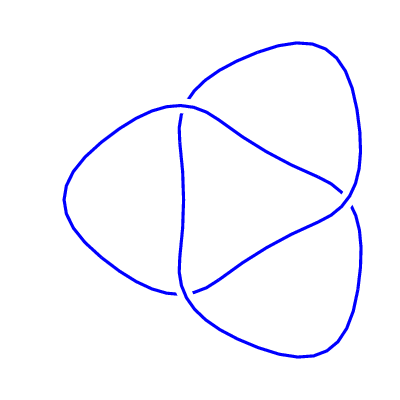
\includegraphics[width=\linewidth]{../data/3_1.png}
        \subcaption{$3_1$}
    \end{minipage}
    \begin{minipage}[b]{.14\linewidth}
        \centering
        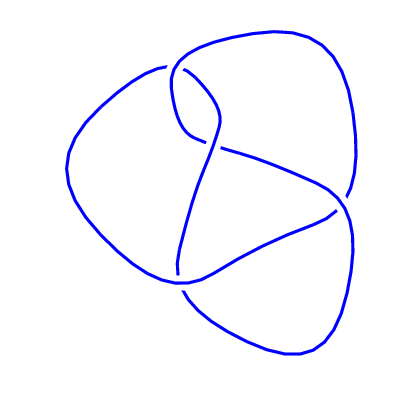
\includegraphics[width=\linewidth]{../data/4_1.png}
        \subcaption{$4_1$}
    \end{minipage}
    \begin{minipage}[b]{.14\linewidth}
        \centering
        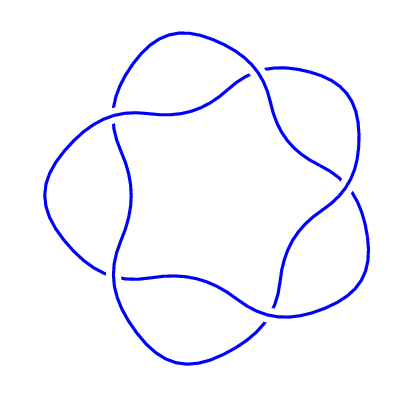
\includegraphics[width=\linewidth]{../data/5_1.png}
        \subcaption{$5_1$}
    \end{minipage}
    \begin{minipage}[b]{.14\linewidth}
        \centering
        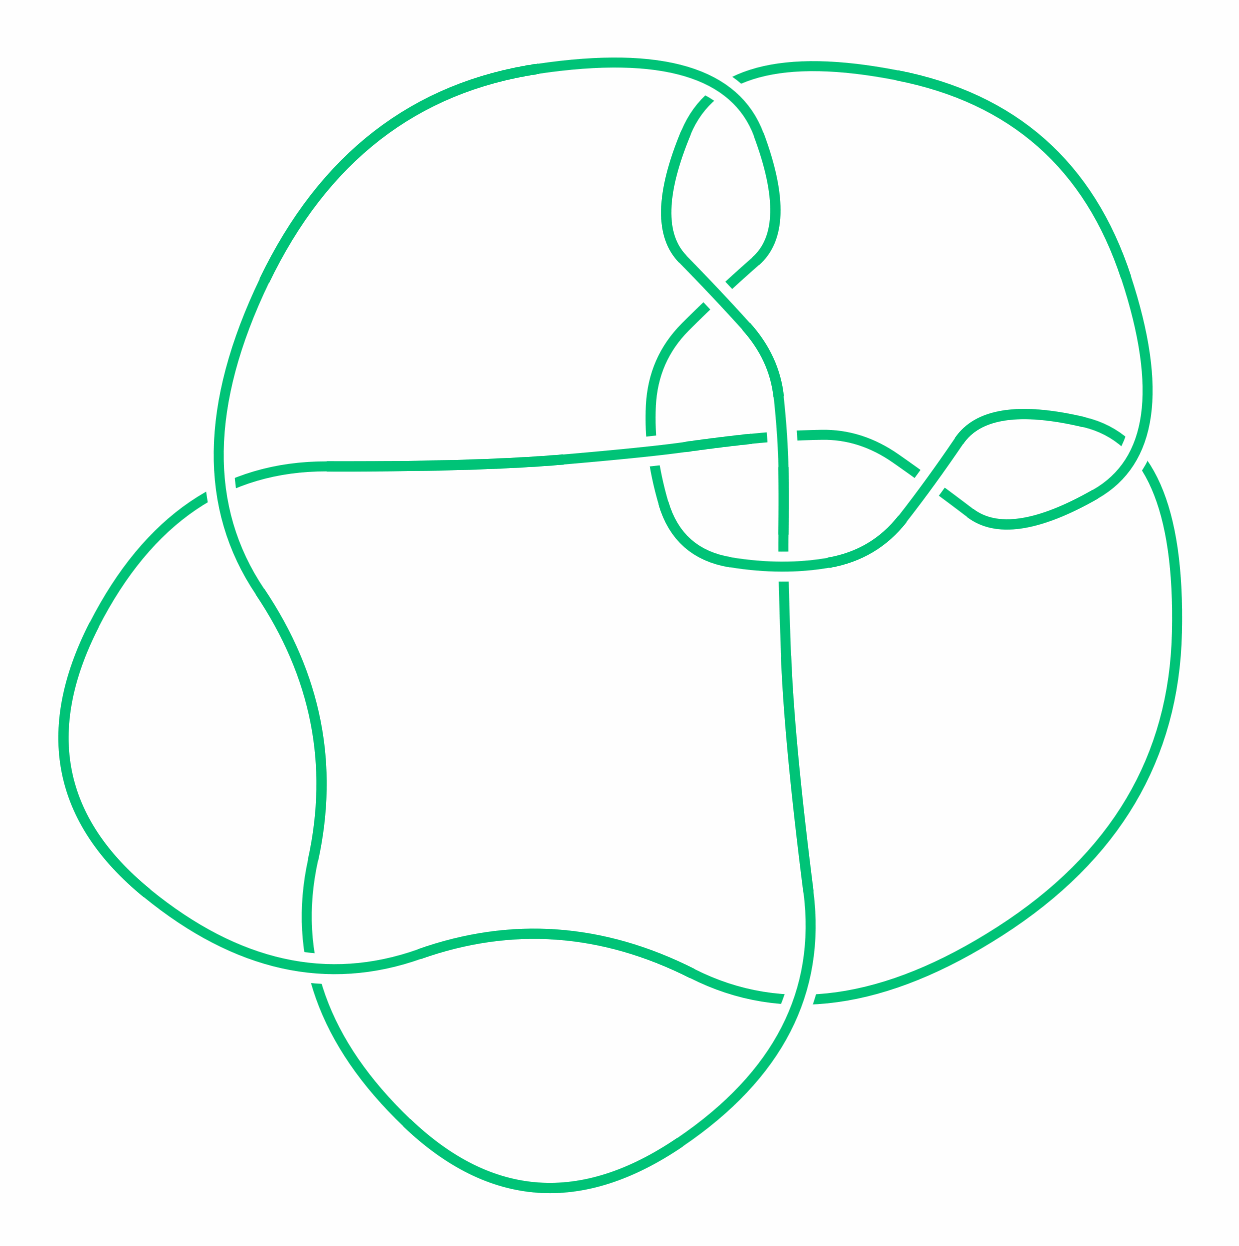
\includegraphics[width=\linewidth]{../data/perko1.png}
        \subcaption{$10_{161}$}
    \end{minipage}
    \begin{minipage}[b]{.14\linewidth}
        \centering
        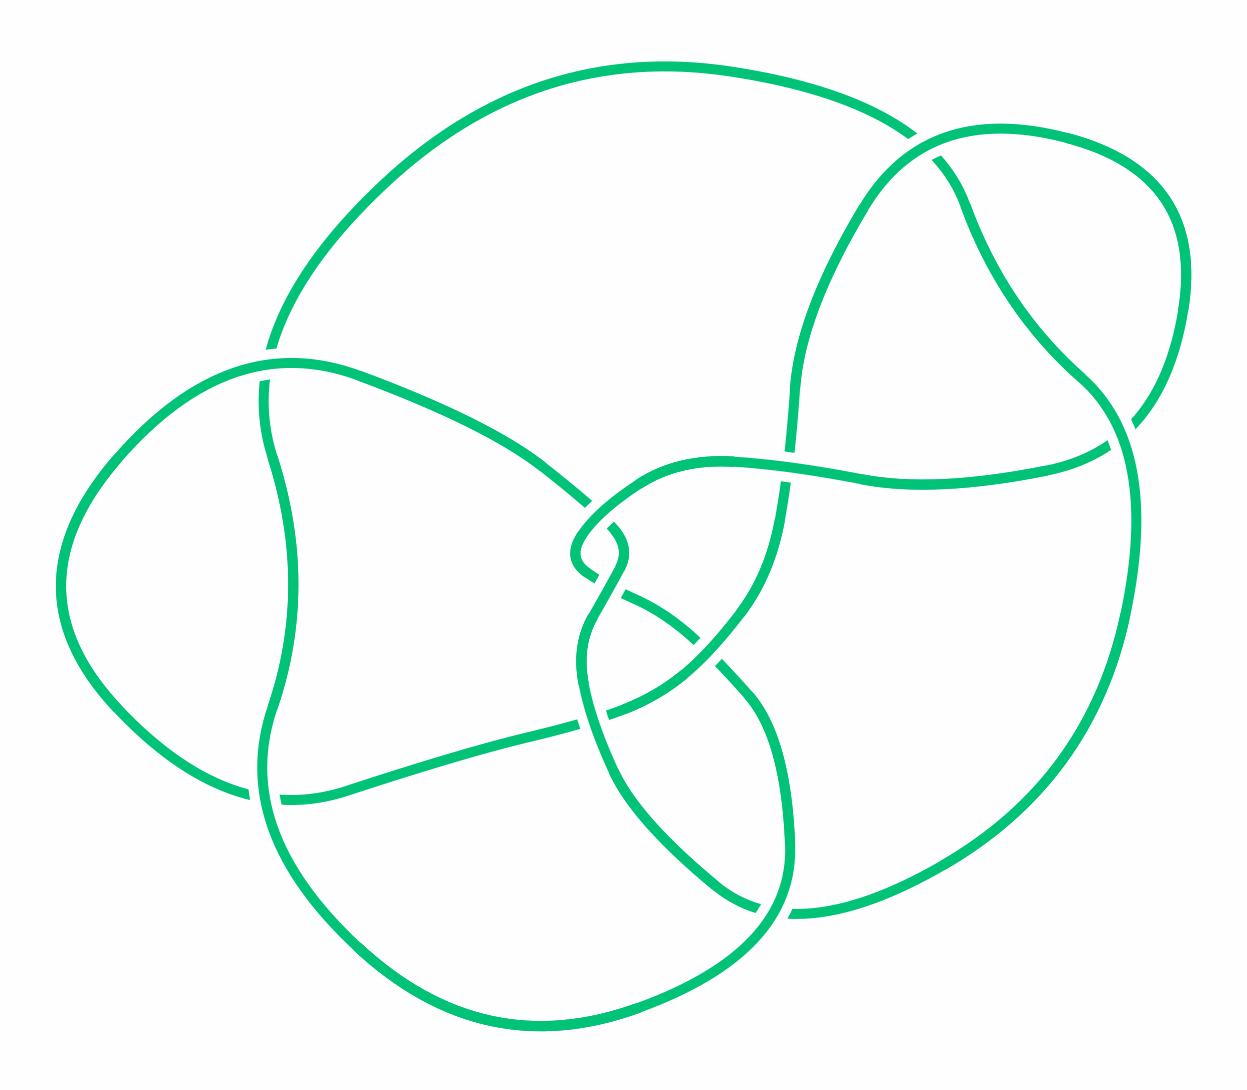
\includegraphics[width=\linewidth]{../data/perko2.png}
        \subcaption{$10_{162}$}
    \end{minipage}
\end{figure}
\end{comment}

Początkowo celem teorii węzłów była klasyfikacja wszystkich węzłów.
Od XIX wieku, kiedy teoria węzłów wyodrębniła się jako osobny dział matematyki,
zdążyliśmy skatalogować ponad sześć miliardów tych obiektów.
Pozornie tak samo wyglądające węzły mogą się od siebie różnić.
Do wykrywania tych subtelnych różnic używa się przede wszystkim niezmienników topologicznych takich jak liczby, wielomiany bądź grupy.
Poznamy je w~dalszych rozdziałach.

Matematycy uogólnili pojęcie węzła:
można rozpatrywać je w~wyższych wymiarach albo zastąpić okrąg inną przestrzenią topologiczną.
Będziemy starać się unikać tych uogólnień.

% koniec wprowadzenia



\section{Węzły i~sploty}

Wprowadzamy pojęcia węzła i splotu, fundamentalnych obiektów teorii, o której napisana została ta książka.
Oprócz tego podajemy definicję, kiedy dwa węzły lub sploty uznajemy za tożsame oraz uzasadniamy, dlaczego akurat ta definicja jest właściwa.

Istnieją odnogi teorii węzłów, które badają inne, pokrewne obiekty.
Mamy na przykład węzły obramowane:

% DICTIONARY;frame;obramowany;węzeł
% DICTIONARY;framing;obramowanie;-
\begin{definition}[obramowanie]
\index{obramowanie|see {węzeł obramowany}}%
\index{węzeł!obramowany}%
    Każde nieznikające normalne pole wektorowe na splocie nazywamy obramowaniem.
    Jeżeli wszystkie wektory są równoległe do płaszczyzny, na której leży diagram tego splotu, obramowanie nazywamy płaskim\footnote{Po angielsku ,,blackboard framing'', ale nie da się tego sensownie przetłumaczyć...}.
\end{definition}

% Liczba samozaczepienia zorientowanego obramowanego splotu $L$ to indeks zaczepienia tego splotu ze sobą pchniętym w kierunku obramowania, jej wartość to dokładnie spin.

% DICTIONARY;virtual;wirtualny;węzeł
% DICTIONARY;welded;zespawany;węzeł
% DICTIONARY;long;długi;węzeł
Są jeszcze węzły wirtualne, zespawane (iloraz węzłów wirtualnych przez ruch znany jako ,,nadskrzyżowania komutują''), długie (gdzie końce nie są ze sobą zszyte, ale umieszczone tak daleko, że są nieosiągalne) i inne.
\index{węzeł!wirtualny}%
\index{węzeł!zespawany}%
\index{węzeł!długi}%
Ta książka nie zawiera zbyt wiele informacji o wspomnianych bytach.
% TODO wirtualne: 2994594 10.1142/S021821651240007X
% TODO wirtualne: 2191949 https://arxiv.org/pdf/1409.2823.pdf 

\subsection{Węzły}
Matematyczne węzły można traktować jako model elastycznej oraz pozbawionej grubości liny, której luźne końce zostały ze sobą połączone.
Sugeruje to przyjęcie naiwnej definicji:

\begin{definition}[węzeł]
    Ciągłe oraz różnowartościowe odwzorowanie $S^1 \to \R^3$ nazywamy węzłem.
\end{definition}

Takie rozwiązanie nie jest doskonałe, ponieważ oprócz pożądanych (cokolwiek to znaczy) węzłów, obejmuje wiele innych, patologicznych obiektów takich jak ten z~rysunku \ref{fig_wild_knot}.

\begin{figure}[H]
    \centering
\begin{comment}
    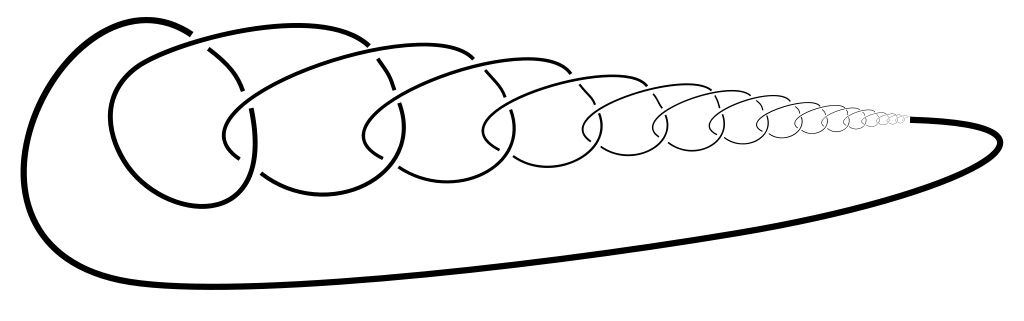
\includegraphics[width=0.44\linewidth]{wild_knot.png}
\end{comment}
    \caption[caption-for-lof-1]{Węzeł dziki, źródło: Wikimedia{\footnotemark}.}
    \label{fig_wild_knot}
\end{figure}
\footnotetext{\url{https://upload.wikimedia.org/wikipedia/commons/2/2f/Wildknot.svg}}

Zamiast wyjaśnić, jakie są jego niepożądane właściwości, podamy od razu dobrą definicję.
Można dodać założenie o tym, że pochodna odwzorowania $S^1 \to \R^3$ nie znika w żadnym punkcie, albo ograniczyć się do łamanych:

\begin{definition}[węzeł]
    Różnowartościowe odwzorowanie $S^1 \to \R^3$, którego pochodna istnieje i nie znika w żadnym punkcie, nazywamy węzłem.
\end{definition}

% DICTIONARY;knot;węzeł;-
% DICTIONARY;tame;poskromiony;węzeł
% DICTIONARY;wild;dziki;węzeł
\begin{definition}[węzeł?]
\index{węzeł}%
\label{def:knot}%
    Gładkie włożenie $S^1 \to \R^3$ otaczająco izotopijne z~zamkniętą łamaną bez samoprzecięć nazywamy węzłem poskromionym.
    Dwa węzły są równoważne, jeśli istnieje pomiędzy nimi izotopia otaczająca.
\end{definition}
% TODO: potrzeba jednocześnie gładkości i łamanych?

Czasami wygodniej jest rozpatrywać węzeł jako włożenie $S^1 \to S^3$ albo dopuścić do myśli węzły nieposkromione.
Ale jeśli nie zaznaczono inaczej, nie robimy tego: pisząc węzeł mamy na myśli poskromione włożenie w przestrzeń $\R^3$, nie $S^3$.

Potrzeba jeszcze matematycznego opisu manipulacji, jakim możemy poddawać sznur trzymany w ręce.
Izotopia jest niewłaściwym narzędziem do tego celu: powiedzielibyśmy, że dwa węzły $K_1, K_2$ sa izotopijne, jeśli istnieje ciągła funkcja $F \colon S^1 \times [0, 1] \to \R^3$ taka, że $K_1 = F(-, 0)$ jest pierwszym, zaś $K_2 = F(-,1)$ drugim węzłem (funkcję $F$ nazywa się izotopia).
Tym razem źródło problemów można wskazać jawnie.
Sztuczka Alexandera pozwala usunąć dowolny zaplątany fragment z węzła:

% https://i.stack.imgur.com/QlTxR.png
\begin{figure}[H]
    \centering
\begin{comment}
    
\includegraphics[width=0.44\linewidth]{../data/missing.jpg}
\end{comment}
    \caption[caption-for-lof-2]{Sztuczka? Alexandera??}
\end{figure}

W podobny sposób moglibyśmy przekształcić dowolny węzeł w~niewęzeł.
Teoria, w~której wszystkie obiekty są takie same, nie jest zbyt ciekawa.
Od izotopii należy wymagać gładkości albo lokalnej płaskości,
% https://math.stackexchange.com/questions/1311865/equivalence-of-knots-ambient-isotopy-vs-homeomorphism
co zdaje się prowadzić do pojęcia izotopii otaczającej, która uwzględnia nie tylko sam węzły, ale też to, jak leżą w otaczającej je przestrzeni.

% DICTIONARY;isotopy;izotopia;-
% DICTIONARY;ambient;otaczająca;izotopia
\begin{definition}[izotopia otaczająca]
\index{izotopia otaczająca}%
    Niech $N, M$ będą rozmaitościami, zaś $K_1, K_2 \colon N \to M$ włożeniami.
    Ciągłe odwzorowanie $F \colon M \times [0,1] \to M$ spełniające następujące warunki:
    \begin{enumerate}
        \item funkcja $F(-, 0)$ jest odwzorowaniem tożsamościowym,
        \item każda z funkcji $F(-, t)$ jest homeomorfizmem,
        \item złożenie $F(-, 1)$ z pierwszym włożeniem $K_1$ daje drugie włożenie $K_2$
    \end{enumerate}
    nazywamy izotopią otaczającą przenoszącą $K_1$ na $K_2$.
\end{definition}

W topologii rozważa się włożenia dowolnych rozmaitości, nam wystarczy jeden szczególny przypadek $N = S^1$ oraz $M = \R^3$.
Intuicyjnie, funkcja $F$ zniekształca przestrzeń $\R^3$ tak, że w~chwili początkowej $t = 0$ widzimy pierwszy, zaś w~chwili końcowej $t = 1$ drugi węzeł.
Izotopia otaczająca nie pozwala na ściąganie zaplątanych fragmentów do punktu.

Formalnie węzły to pewne odwzorowania, więc prawidłowym sposobem na zapisanie, że są izotopijne (czyli dla nas: równe), jest $K_1 \cong K_2$.
Ponieważ nie prowadzi to do problemów, będziemy jednak stosować zapis $K_1 = K_2$.
Jednocześnie często węzeł jako odwzorowanie nie będzie odróżniany od obrazu tego odwzorowania.

Istnieje jeszcze jedna, konkurencyjna definicja węzłów równoważnych:

\begin{proposition}
\label{def:equivalent_knots_2}%
    Dwa węzły są równoważne wtedy i tylko wtedy, gdy jeden z~nich jest obrazem drugiego przez zachowujący orientację homeomorfizm $\R^3 \to \R^3$.
\end{proposition}

\begin{proof}
\index[persons]{Milnor, John}%
    Podany niżej dowód pochodzi z~książki ,,Topology from the differentiable viewpoint'' Johna Milnora\footnote{John Willard Milnor zajmuje się głównie topologią różniczkową oraz algebraiczną K-teorią; jego główne dokonania w świecie węzłów to wprowadzenie niezmienników Milnora, które uogólniają grupę podstawową dopełnienia oraz pewne wyniki dotyczące hipotezy plastrowo-taśmowej.}.
\index[persons]{Milnor, John}%
    Musimy pokazać, że dyfeomorfizm $f \colon \R^m \to \R^m$ jest gładko izotopijny z~identycznością.
    Translacje są izotopiami, więc bez straty ogólności zakładamy, że $f(0) = 0$.
    Pochodna $f$ w~zerze jest dana wzorem $\mathrm{d}f_0(x) = \lim_{t \to 0} f(tx) /t$,
    naturalną definicję izotopii $F \colon \R^m \times [0, 1] \to \R^m$ stanowi więc
    \begin{equation}
        F(x, t) = \begin{cases}
            \mathrm{d}f_0(x) & t = 0 \\
            f(tx) / t & 0 < t \le 1
        \end{cases} .
    \end{equation}

    Na mocy lematu Hadamarda funkcja $f$ zapisuje się jako suma $x_1 g_1(x) + \ldots + x_mg_m(x)$, gdzie funkcje $g_i$ są gładkie, więc funkcja $F$ też jest gładka, co jakoś kończy dowód.
\end{proof}

Milnor zauważa, że istnieje dyfeomorfizm $S^6 \to S^6$ stopnia $+1$, który nie jest gładko izotopijny z~identycznością!

\subsection{Sploty}
% DICTIONARY;link;splot;-
% DICTIONARY;component;ogniwo splotu;-
\begin{definition}[splot, ogniwo]
\index{splot}%
    Sumę parami rozłącznych węzłów
    \begin{equation}
        L = K_1 \sqcup K_2 \sqcup \ldots K_n
    \end{equation}
    nazywamy splotem, a~składniki sumy -- ogniwami.
\end{definition}

Przez analogię do węzłów mówimy, że dwa sploty są takie same, jeśli jeden jest obrazem drugiego przez zachowujący orientację homeomorfizm $\R^3 \to \R^3$.
W~takiej sytuacji obydwa sploty mają tyle samo ogniw.

\begin{example}
\index{splot!Hopfa}%
\index[persons]{Hopf, Heinz}%
    Splot Hopfa\footnote{Heinz Hopf był niemiecko-szwajcarskim pionierem topologii algebraicznej. W~1931 roku zajmował się splotem Hopfa w ramach badań nad tzw. rozwłóknieniem \emph{(Hopf fibration)}.} to najprostszy splot nietrywialny.
\end{example}

\begin{example}
\index{splot!Whiteheada}%
\index[persons]{Whitehead, John}%
    Splot Whiteheada\footnote{John Henry Constantine Whitehead był jednym z założycieli teorii homotopii. Oprócz wspomnianego tu splotu Whiteheada zobaczymy jego nazwisko jeszcze raz, przy dublu Whiteheada.} ma dwa ogniwa i w~1934 służył Whiteheadowi za kontrprzykład do nieudanego dowodu (także Whiteheada!) hipotezy Poincarego.
\end{example}

\begin{comment}
    \begin{figure}[H]
        \begin{minipage}[b]{.48\linewidth}
            \centering
            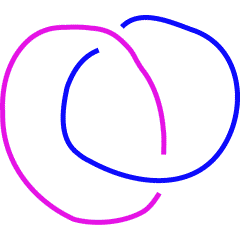
\includegraphics[width=0.5\linewidth]{../data/mixed/L2a1.png}
            \subcaption{splot Hopfa}
        \end{minipage}
        \begin{minipage}[b]{.48\linewidth}
            \centering
            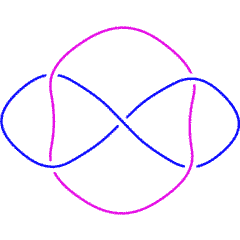
\includegraphics[width=0.5\linewidth]{../data/mixed/L5a1.png}
            \subcaption{splot Whiteheada}
        \end{minipage}
    \end{figure}
\end{comment}

% TODO: przesunąć to gdzieś dalej, za definicję skrzyżowania
Poniższa definicja nie jest nam jeszcze potrzebna, ale wygodnie przytoczyć ją już teraz.

% DICTIONARY;splittable;rozszczepialny;splot
\begin{definition}[rozszczepialność]
\index{splot!rozszczepialny}%
    Jeżeli splot $L$ można zanurzyć w przestrzeni $\R^3$ tak, że niektóre jego ogniwa będą leżeć nad pewną rozłączną ze splotem płaszczyzną, zaś pozostałe pod nią, to powiemy, że splot $L$ jest rozszczepialny.
\end{definition}

Liczbę nierozszczepialnych splotów pierwszych zebrano w~tabeli:

\renewcommand*{\arraystretch}{1.4}
\footnotesize
\begin{longtable}{lcccccccccccc}
    \hline
    \textbf{skrzyżowania} & 0 & 1 & 2 & 3 & 4 & 5 &  6 &  7 &  8 & 9 & 10 & 11 \\ \hline \endhead
    sploty pierwsze, nierozszczepialne & 0 & 0 & 1 & 0 & 1 & 1 & 6 & 9 & 29 & 83 & 287 & 1007 \\
    (w tym) alternujące & 0 & 0 & 1 & 0 & 1 & 1 & 5 & 7 & 21 & 55 & 174 & 548 \\
    (w tym) niealternujące & 0 & 0 & 0 & 0 & 0 & 0 & 1 & 2 & 8 & 28 & 113 & 459 \\
    \hline
\end{longtable}
\normalsize

W bazie danych OEIS można trafić na ciąg \href{https://oeis.org/A086826}{A086826} opisujący liczbę nierozszczepialnych pierwszych i złożonych węzłów i splotów.
Powyższa tabela zawiera liczby na podstawie portalu LinkInfo \cite{linkinfo23}.
Odpowiedź na pytanie ,,czym są skrzyżowania?'' przynosi definicja \ref{def:crossing}.

Pewne kryteria rozszczepialności konkretnych splotów znaleźć można u Kawauchiego \cite[s. 36-38]{kawauchi96}.

\subsection{Dopełnienia węzłów i splotów}

Jeśli dwa węzły są równoważne, to ich dopełnienia są oczywiście homeomorficzne.
Pytanie o~prawdziwość implikacji odwrotnej jako pierwszy zadał najprawdopodobniej Tietze \cite{tietze08} w~1908 roku.
\index[persons]{Tietze, Heinrich}%
W roku 1987 pokazano, że istnieją co najwyżej dwa węzły o~zadanym dopełnieniu (Culler, Gordon, Luecke, Shalen \cite{culler87}).
\index[persons]{Culler, Marc}%
\index[persons]{Shalen, Peter}%
\index[persons]{Gordon, Cameron}%
\index[persons]{Luecke, John}%
Dwa lata później poznaliśmy pozytywną odpowiedź na pytanie Tietzego: każdy węzeł jest wyznaczony jednoznacznie przez swoje dopełnienie.

\begin{theorem}[Gordon, Luecke, 1989]
\index[persons]{Gordon, Cameron}%
\index[persons]{Luecke, John}%
\index{twierdzenie!Gordona-Lueckego}%
    Poskromione węzły o~homeomorficznych (z zachowaniem orientacji) dopełnieniach są wzajemnie izotopijne.
\end{theorem}

\begin{proof}[Niedowód]
    Wynika to z teorii Cerfa, kombinatorycznych technik w stylu Litherlanda, cienkich pozycji, cykli Scharlemanna i~ogólniejszego stwierdzenia: nietrywialna chirurgia Dehna na węźle w~3-sferze nigdy nie daje 3-sfery.
% https://en.wikipedia.org/wiki/Gordon–Luecke_theorem: Essential ingredients of the proof are their joint work with Marc Culler and Peter Shalen on the cyclic surgery theorem, combinatorial techniques in the style of Litherland, thin position, and Scharlemann cycles.
\index{chirurgia Dehna}%
\index{teoria Cerfa}%
\index{cykle Scharlemanna}%
    Pełny dowód zawiera praca \cite{gordon89}.
\end{proof}

Twierdzenie to zamienia problem lokalny (czy dwa węzły w kuli $S^3$ są równoważne?) na problem globalny (czy dwie przestrzenie topologiczne są homeomorficzne?).
Jego odpowiednik dla splotów jest fałszywy i wiedziano o tym od bardzo dawna: w~1937 roku Whitehead \cite{whitehead37} podał nieskończenie wiele splotów, których dopełnienia wyglądają jak dopełnienia splotu Whiteheada.
\index[persons]{Whitehead, John}%

% koniec sekcji Węzły i sploty



\section{Diagramy. Ruchy Reidemeistera}

Chociaż w~świetle definicji \ref{def:knot} węzły są pewnymi regularnymi podzbiorami przestrzeni $\R^3$, z~kombinatorycznego punktu widzenia wygodniej jest rysować je na płaszczyźnie.

\begin{definition}[orientacja]
\index{węzeł!zorientowany}%
\index{orientacja|see {węzeł zorientowany}}%
    Węzeł, w~którym wybrano kierunek, w~którym należy się po nim poruszać, nazywamy zorientowanym.
    Splot nazywamy zorientowanym, jeśli wszystkie jego ogniwa traktowane jako węzły są zorientowane.
\end{definition}

Orientację na diagramie zaznaczamy małą strzałką wskazującą kierunek poruszania się.

\begin{definition}
\index{cień}%
    Rzut węzła $K \subseteq \R^3$ na płaszczyznę nazywamy cieniem.
\end{definition}

\begin{definition}[skrzyżowanie]
\index{skrzyżowanie}% 
    Podwójny punkt w cieniu nazywamy skrzyżowaniem.
\end{definition}

\begin{definition}[diagram]
\index{diagram}%
    Cień razem z~informacją o~tym, jak przebiegają skrzyżowania i pozbawiony katastrof: potrójnych przecięć, stycznych czy dziobów nazywamy diagramem.
    % TODO: Narysować katastrofy
\end{definition}

\begin{definition}[włókno]
\index{włókno}%
    Fragment diagramu, który biegnie między dwoma kolejnymi tunelami, czyli podskrzyżowaniami, nazywamy włóknem.
\end{definition}

\begin{definition}[nić]
\index{nić}%
    Fragment diagramu, który biegnie między dwoma kolejnymi skrzyżowaniami, nazywamy nicią.
\end{definition}

Nici powstają z włókien przez rozcięcie ich przy każdym nadskrzyżowaniu.

\begin{proposition}
    Niech $L$ będzie splotem.
    Jego diagramy tworzą otwarty i~gęsty podzbiór wszystkich rzutów.
\end{proposition}

Kawauchi \cite[s. 7]{kawauchi96} wspomina w tym miejscu podręcznik Crowella, Foxa \cite[s. 7]{crowell63}.
To samo jest na przykład w~\cite[s. 10]{burde14}.

\begin{proof}
    Rzut splotu na równoległe płaszczyzny jest taki sam, a te można sparametryzować prostymi przechodzącymi przez początek układu współrzędnych, które tworzą przestrzeń rzutową $\R \mathbb P^2$.
    Niech $S$ będzie zbiorem prostych, które dają złe rzuty.
    Wystarczy pokazać jego nigdziegęstość.
    Okazuje się, że $S$ jest też jednowymiarowy.
\end{proof}

\begin{corollary}
    Każdy splot posiada diagram.
\end{corollary}

Każdy węzeł ma zatem wiele diagramów; mając dane dwa różne chcielibyśmy wiedzieć, czy przedstawiają ten sam węzeł.
Kurt Reidemeister podał proste kryterium rozstrzygające ten problem w~latach dwudziestych ubiegłego wieku.
Najpierw zdefiniujmy trzy lokalne operacje na diagramach.

\begin{definition}[ruchy Reidemeistera]
\index{ruchy Reidemeistera}%
    Trzy gatunki lokalnych deformacji diagramu splotu:
\begin{comment}
    \[
        \underbrace{\begin{tikzpicture}[baseline=-0.65ex,scale=0.1]
        \begin{knot}[clip width=5]
            \strand[thick] (-5, 10) to [in=left, out=down] (2, -5);
            \strand[thick] (5, 0) to [in=right, out=down] (2, -5);
            \strand[thick] (5, 0) to [in=right, out=up] (2, 5);
            \strand[thick] (-5, -10) to [in=left, out=up] (2, 5);
        \end{knot}
        \end{tikzpicture}
        \, \cong \,
        \begin{tikzpicture}[baseline=-0.65ex,scale=0.1]
        \begin{knot}[clip width=5]
            \strand[thick] (0,10) to (0,-10);
        \end{knot}
        \end{tikzpicture}}_{R_1}
        %%%
        \quad \quad \quad
        \underbrace{\begin{tikzpicture}[baseline=-0.65ex,scale=0.1]
        \begin{knot}[clip width=5]
            \strand[thick] (-5, 10) to [in=up, out=down] (5, 0);
            \strand[thick] (-5, -10) to [in=down, out=up] (5, 0);
            \strand[thick] (5, 10) to [in=up, out=down] (-5, 0);
            \strand[thick] (5, -10) to [in=down, out=up] (-5, 0);
        \end{knot}
        \end{tikzpicture}
        \, \cong \,
        \begin{tikzpicture}[baseline=-0.65ex,scale=0.1]
        \begin{knot}[clip width=5]
            \strand[thick] (-5, 10) to [in=up, out=down] (-2, 0);
            \strand[thick] (-5, -10) to [in=down, out=up] (-2, 0);
            \strand[thick] (5, 10) to [in=up, out=down] (2, 0);
            \strand[thick] (5, -10) to [in=down, out=up] (2, 0);
        \end{knot}
        \end{tikzpicture}}_{R_2}
        %%%
        \quad \quad \quad
        \underbrace{\begin{tikzpicture}[baseline=-0.65ex,scale=0.1]
        \begin{knot}[clip width=5, flip crossing/.list={1,2,3}]
            \strand[thick] (-10, -10) -- (10, 10);
            \strand[thick] (-10, 10) -- (10, -10);
            \strand[thick] (-10, 0) to [in=left, out=right] (0, 10);
            \strand[thick] (10, 0) to [in=right, out=left] (0, 10);
        \end{knot}
        \end{tikzpicture}
        \, \cong \,
        \begin{tikzpicture}[baseline=-0.65ex,scale=0.1]
        \begin{knot}[clip width=5, flip crossing/.list={1,2,3}]
            \strand[thick] (-10, -10) -- (10, 10);
            \strand[thick] (-10, 10) -- (10, -10);
            \strand[thick] (-10, 0) to [in=left, out=right] (0, -10);
            \strand[thick] (10, 0) to [in=right, out=left] (0, -10);
        \end{knot}
        \end{tikzpicture}}_{R_3}
    \]
\end{comment}
    skręcenie lub rozkręcenie ($R_1$), wsunięcie lub rozsunięcie ($R_2$) oraz przesunięcie łuku przez skrzyżowanie ($R_3$) nazywamy ruchami Reidemeistera.
\end{definition}

Ruch $R_i$ operuje więc na $i$ łukach diagramu.
Reidemeister w~swojej pierwszej pracy przyjął inną kolejność, jego drugi ruch jest naszym pierwszym.

\begin{theorem}[Reidemeister, 1927]
\label{thm:reidemeister}%
\index{twierdzenie!Reidemeistera}%
    Niech $D_1, D_2$ będą diagramami dwóch splotów $L_1, L_2$.
    Sploty $L_1, L_2$ są takie same wtedy i tylko wtedy, gdy diagram $D_2$ można otrzymać z $D_1$ wykonując skończony ciąg ruchów Reidemeistera oraz gładkich deformacji łuków, bez zmiany biegu skrzyżowań.
\end{theorem}

Dowód podali niezależnie Reidemeister \cite{reidemeister27} oraz Alexander, Briggs \cite{briggs27}.
Twierdzenie Reidemeistera jest prawdziwe także dla splotów zorientowanych, wtedy jednak w każdym ruchu trzeba uwzględnić wszystkie możliwe orientacje łuków.

\begin{proof}
    Szkielet dowodu można znaleźć w~książce Burdego i~Zieschanga \cite[s. 9-11]{burde14}.
    Kluczowe pomysły zawiera też \cite[s. 11-12]{prasolov97} Prasołowa i~Sosińskiego.
    Innym przystępnym źródłem jest podręcznik \cite[s. 50-56]{murasugi96} Murasugiego.
\end{proof}

Trace \cite{trace83} zauważył, że dwa diagramy jednego węzła są związane tylko II i III ruchem (ale nie I) wtedy i tylko wtedy, gdy mają ten sam spin oraz indeks punktu względem krzywej (,,winding number'').
Z prac Östlunda \cite{ostlund01}, Manturowa\footnote{Niestety nie wiem, o które strony tej książki chodzi.} \cite{manturov04} oraz Haggego \cite{hagge06} wynika, że dla każdego węzła istnieje para diagramów, do przejścia między którymi trzeba wykorzystać wszystkie trzy ruchy.
% praca Haggego nazywa się "Every Reidemeister move is needed for each knot type" ale nawet w MathSciNecie wspomnieni są Ostlund i Manturow, więc zostawiam. Tekst skopiowany z Wiki
Coward \cite{coward06} zademonstrował, że nawet jeśli wszystkie trzy ruchy są potrzebne, można je wykonywać w specjalnej kolejności: najpierw tylko I ruchy, potem tylko II ruchy, następnie tylko III ruchy i znowu II ruchy.

W praktyce twierdzenia \ref{thm:reidemeister} nie stosuje się bezpośrednio do diagramów splotów.
Mając dane dwa spójne diagramy tego samego splotu trudno znaleźć jest ciąg ruchów przekształcający jeden z nich w drugi.
Załóżmy, że widać na nich odpowiednio $n_1, n_2$ skrzyżowań.
Jak piszą Coward, Lackenby w \cite{coward11}, istnieje funkcja $f \colon \N \times \N \to \N$ taka, że między dwoma diagramami można przejść wykonując co najwyżej $f(n_1, n_2)$ ruchów.
Wynika to z oczywistego faktu, że istnieje skończenie wiele spójnych diagramów o danej liczbie skrzyżowań oraz twierdzenia Reidemeistera.
Okazuje się jednak, że od funkcji $f$ można żądać, by była obliczalna i faktycznie, główny wynik \cite{coward11} orzeka, że
\begin{equation}
    f(n_1, n_2) = 2^{2^{\ldots^{2^{n_1 + n_2}}}}
\end{equation}
jest taką funkcją.
Piętrowa potęga liczy sobie aż $10^{1000000 (n_1 + n_2)}$ warstw, ale przynajmniej jest jawnie zdefiniowana.
Natomiast jeżeli $n_2 = 0$, czyli drugi diagram przedstawia niewęzeł, wystarcza $(236n_1)^{11}$ ruchów, to świeższy wynik samego Lackenby'a \cite{lackenby15}.

\begin{tobedone}
    Przedstawić rozumowanie (piramidka z węzłami), dlaczego to nie jest takie oczywiste.
\end{tobedone}

Hayashi \cite{hayashi05} dowiódł, że liczbę ruchów Reidemeistera potrzebnych, by rozszczepić splot można ograniczyć z góry na podstawie indeksu skrzyżowaniowego.

Zamiast tego definiuje się niezmienniki, czyli funkcje ze zbioru wszystkich diagramów, które nie zmieniają swojej wartości podczas wykonywania ruchów Reidemeistera.
Kiedy pewien niezmiennik przyjmuje różne wartości na dwóch diagramach, te przedstawiają dwa istotnie różne sploty.
Gdy wartości są te same, nie dostajemy żadnej informacji.
Sploty mogą być równoważne albo nie.
Niezmienniki będą nam stale towarzyszyć w~wędrówce po krainie węzłów.

% koniec sekcji Ruchy Reidemeistera

Wolfgang Haken \cite{haken61} podał przepis na wykrycie diagramu niewęzła i rozwiązał częściowo jeden z~ważniejszych problemów teorii węzłów.
Długo nikt nie podjął się implementacji tego algorytmu\footnote{Moritz Epple pisze ,,this algorithm was extremely impractical''.}, udało się to Burtonowi, Budneyowi oraz Petterssonowi w~komputerowym programie Regina\footnote{Dostępny pod adresem \url{https://regina-normal.github.io/}.} na przełomie tysiącleci.
Burton, Rubinstein i~Tillman pokazali w~pracy \cite{burton12}, jak sprawdzać, czy powierzchnia normalna na striangulowanej 3-rozmaitości jest (nie)ściśliwa w~czasie wykładniczym.
To okazało się wystarczyć do udzielenia negatywnej odpowiedzi na pytanie Thurstona: ,,czy przestrzeń Seiferta-Webera jest rozmaitością Hakena?'', a zatem wykraczającego poza poziom tej pracy.
\index{przestrzeń Seiferta-Webera}%
\index{rozmaitość Hakena}%

SnapPea\footnote{Dostępny pod adresem \url{http://geometrygames.org/SnapPea/index.html}.} to inny popularny wśród niskowymiarowych topologów program pozwalający badać hiperboliczne 3-rozmaitości, patrz sekcja \ref{sec:hyperbolic}.

Wiadomo, że genus wykrywa niewęzły (fakt \ref{prp:genus_detects_unknot}) i nie wiadomo, czy wielomian Jonesa to robi (hipoteza \ref{con:jones}).
\index{genus}%
\index{wielomian Jonesa}%

Przykładami trudnych w~rozpoznaniu niewęzłów są: niewęzeł Goritza, Freedmana.
Więcej trudnych niewęzłów zawiera praca \cite{zanellati16} autorstwa Petronio oraz Zanellatiego.

\index{niewęzeł}
\index{niewęzeł!Goritza}
\index{niewęzeł!Freedmana}
\begin{comment}
\begin{figure}[H]
    \begin{minipage}[b]{.32\linewidth}
        \centering
        
\includegraphics[width=\linewidth]{../data/missing.jpg}
        \subcaption{normalny}
    \end{minipage}
    \begin{minipage}[b]{.32\linewidth}
        \centering
        
\includegraphics[width=\linewidth]{../data/missing.jpg}
        \subcaption{Goritza}
    \end{minipage}
    \begin{minipage}[b]{.32\linewidth}
        \centering
        
\includegraphics[width=\linewidth]{../data/missing.jpg}
        \subcaption{Freedmana}
    \end{minipage}
\end{figure}
\end{comment}

Zanim opowiemy, jak dotąd przebiegała klasyfikacja węzłów o małej liczbie skrzyżowań, zdefiniujemy klasę splotów ze specjalnymi diagramami.

\begin{definition}[alternacja]
\index{węzeł!alternujący}%
    Diagram splotu, gdzie podczas poruszania się wzdłuż każdego ogniwa nad- oraz podskrzyżowania mijane są naprzemiennie, nazywamy alternującym.
    Splot jest alternujący, jeśli posiada alternujący diagram.
\end{definition}

Około 1961 roku Fox zapytał ,,What is an alternating knot?''.
Szukano takiej definicji węzła alternującego, która nie odnosi się bezpośrednio do diagramów, aż w~2015 roku Joshua Greene podał geometryczną charakteryzację: nierozdzielczy splot w $S^3$ jest alternujący wtedy i tylko wtedy, gdy ogranicza dodatnią oraz ujemną określoną powierzchnię rozpinającą \cite{greene17}.
% definite spanning surface

Sundberg oraz Thistlethwaite pokazali w 1998 roku, że liczba splotów alternujących rośnie wykładniczo (\cite{sundberg98}):

\begin{proposition}
    Niech $a_n$ oznacza liczbę pierwszych, alternujących supłów o~$n$ skrzyżowaniach.
\index{supeł}%
    Wtedy
    \begin{equation}
        a_n \sim (3c_1/4\sqrt{\pi})n^{-5/2}\lambda^{n-3/2},
    \end{equation}
    gdzie zarówno $c_1$, pierwszy współczynnik rozwinięcia Taylora funkcji $\Phi(\eta)$ zdefiniowanej w \cite{sundberg98}, jak i $\lambda$ są jawnie znanymi stałymi:
    \begin{align}
        c_1 & = \sqrt{\frac{5^7 \cdot (21001 + 371 \sqrt{21001})^3}{2 \cdot 3^{10} \cdot (17 + 3\sqrt{21001})^5}} \\
        \lambda & = \frac {1}{40} (101 + \sqrt{21001})
    \end{align}
    Niech $A_n$ oznacza liczbę pierwszych, alternujących splotów o $n$ skrzyżowaniach.
    Wtedy $A_n \approx \lambda^n$, dokładniej: jeśli $n \ge 3$, to
    \begin{equation}
        \frac{a_{n-1}}{16n - 24} \le A \le \frac{a_n - 1}{2}.
    \end{equation}
\end{proposition}

Czasami będziemy używać słów przed ich zdefiniowaniem, tak jak uczyniliśmy tutaj: węzły pierwsze i~supły pojawiają się odpowiednio w definicjach \ref{def:prime_knot}, \ref{def:tangle}.
Książkę trzeba więc przeczytać co~najmniej dwa razy.

\begin{proposition}
    Niech $a_n$ oznacza liczbę pierwszych, alternujących supłów o~$n$ skrzyżowaniach.
    Wtedy funkcja tworząca $f(z) = \sum_n a_n z^n$ spełnia równanie
    \begin{equation}
    f(1+z) - f(z)^2 - (1+f(z))q(f(z)) -z - \frac{2z^2}{1-z} = 0,
    \end{equation}
    gdzie $q(z)$ jest pomocniczą funkcją
    \begin{equation}
        q(z) = \frac{2z^2 - 10z - 1 + \sqrt{(1-4z)^3}} {2(z+2)^3} - \frac{2}{1+z} -z + 2.
    \end{equation}
\end{proposition}

Powyższa ciekawostka także pochodzi z cytowanej wcześniej pracy \cite{sundberg98}.


\subsection{Historia tablic węzłów}
% DICTIONARY;knot table;tablica węzłów;-
Pierwszą osobą, która podjęła się szukania węzłów, był Peter Guthrie Tait, szkocki fizyk.
Razem z Thomsonem (lordem Kelvinem) wierzyli, że węzły są kluczem do zrozumienia widma spektroskopowego różnych pierwiastków: na przykład atom sodu mógł być splotem Hopfa ze względu na dwie linie emisyjne.
Eksperyment Michelsona-Morleya z 1887 roku zabił ich ,,wirową teorię atomu'', ale nie miało to znaczenia dla teorii węzłów jako działu matematyki.

Używana po dziś dzień strategia, którą przyjął Tait, jest stosunkowa prosta: narysować wszysktie możliwe diagramy o~zadanym indeksie skrzyżowaniowym, po czym połączyć ze sobą te, które przedstawiają jeden węzeł.
Na potrzeby pierwszego etapu Tait wymyślił schemat kodowania diagramów.
Opiszemy później jego ulepszenie, kod Dowkera-Thistlethwaite'a.

Tait wykorzystując swoją notację podał w~1876 pierwszą tablicę piętnastu węzłów o~mniej niż ośmiu skrzyżowaniach.
Nie należy traktować tego jako skromny wynik: nie miał on do dyspozycji żadnych twierdzeń topologicznych do odróżniania węzłów.
Onieśmielony przez liczbę możliwych ciągów dla kolejnych indeksów skrzyżowaniowych, powstrzymał się przed rozszerzaniem swojej tablicy.
To właśnie grupowanie diagramów przedstawiających ten sam węzeł, a~nie samo szukanie wszystkich możliwych diagramów, sprawia trudność.

Aby sobie pomóc, Tait znalazł lokalną modyfikację diagramu, która nie zmienia indeksu skrzyżowaniowego, znaną obecnie\footnote{Dla Taita ,,flype'' było innym ruchem, prostyą transformacją związaną ze zmianą wyboru nieskończonego obszaru, ale mało kto teraz o tym pamięta. Dowiedzieliśmy się o tym z pracy \cite{menasco93}, której autorzy dowiedzieli się o tym od Claude'a Webera.} jako flype.
\index{flype}
Flype to stary szkocki czasownik oznaczający ,,wykręcać na drugą stronę''.

\begin{comment}
\[
\begin{tikzpicture}[baseline=-0.65ex, scale=0.1]
\begin{knot}[clip width=5, end tolerance=1pt, flip crossing/.list={1}]
    \strand[semithick] (-21, -5) [in=180, out=0] to (-7, 5);
    \strand[semithick] (-21, 5) [in=180, out=0] to (-7, -5);
    \draw (-7, -7) rectangle (7, 7);
    \node at (0, 0) {\Huge {$T$}};
    \draw[semithick] (7, -5) to (21, -5);
    \draw[semithick] (7, 5) to (21, 5);
\end{knot}
\end{tikzpicture}
\quad \cong_{\mathrm{flype}} \quad
\begin{tikzpicture}[baseline=-0.65ex, scale=0.1]
\begin{knot}[clip width=5, end tolerance=1pt]
    \strand[semithick] (21, -5) [in=0, out=180] to (7, 5);
    \strand[semithick] (21, 5) [in=0, out=180] to (7, -5);
    \draw (-7, -7) rectangle (7, 7);
    \node at (0, 0) {\rotatebox[origin=c]{-180}{\Huge $T$}};
    \draw[semithick] (-7, -5) to (-21, -5);
    \draw[semithick] (-7, 5) to (-21, 5);
\end{knot}
\end{tikzpicture}
\]
\end{comment}

Inną taktykę szukania węzłów przyjał wielebny Thomas Kirkman\footnote{Oto jak Kirkman definiował węzeł w stu słowach: ,,By a Knot of $n$ crossings, I understand a reticulation of any number of meshes of two or more edges, whose summits, all tessaraces, are each a single crossing, as when you cross your forefingers straight or slightly curved, so as not to linK them, and such meshes that every thread is either seen, when the projection of the Knot with its $n$ crossings and no more is drawn in double lines, or conceived by the reader of its course when drawn in single line, to pass alternately under and over the threads to which it comes at successive crossings.''}: zaczynał od małego zbioru "nieredukowalnych" rzutów, do których systematycznie dokładał skrzyżowania.
% wielebny => Adams, s. 31
Tait przeczytał pracę Kirkmana, po czym w~latach 1884/1885 opracował listę węzłów alternujących o~mniej niż 11 skrzyżowaniach.
% Kirkman miał wtedy 78 lat!
Tuż przed oddaniem jej do druku odkrył inny spis węzłów stworzony przez amerykańskiego naukowca Charlesa Little'a.
Znalazł wtedy jeden duplikat u~siebie, natomiast u Little'a jeden duplikat i~jedno pominięcie.

Zachęcony przez Taita, Little zabrał się za alternujące węzły o~11 skrzyżowaniach i~za trudniejsze zadanie, stablicowanie węzłów niealternujących, czyli takich, które nie posiadają alternującego diagramu.
Jak wynika z~pierwszej pracy Taita, początkowo nie wierzono, że takie w~ogóle istnieją.
Dowód znaleziono wiele lat później, niealternujące są $8_{19}$, $8_{20}$, $8_{21}$, ale nie pierwsze węzły o mniejszej liczbie skrzyżowań.
Patrz twierdzenie \ref{prp:bankwitz}.
Little pracował przez sześć lat (1893 -- 1899) i~znalazł 43 niealternujące węzły o~10 skrzyżowaniach.
Żadnego nie pominął, ale trafił mu się jeden duplikat.

W kolejnych dziesięcioleciach nie nastąpił znaczący postęp, zarówno w~rozszerzaniu tablic jak i~sprawdzaniu tych już istniejących.
Haseman w~1918 roku znalazła achiralne węzły o~12 i~14 skrzyżowaniach \cite{haseman18}.
W 1927 roku Alexander z~Briggsem przy użyciu pierwszej grupy homologii rozgałęzionego nakrycia cyklicznego (!) potrafili odróżnić od siebie dowolne dwa węzły (z~pominięciem 3 par) o~co najwyżej 9 skrzyżowaniach \cite{briggs27}.
Reidemeister poradził sobie z~tymi wyjątkami w~1932 roku, korzystając z~indeksu zaczepienia i~homomorfizmów z~grupy węzła na grupy diedralne \cite{reidemeister32}.
% branch curves in irregular covers associated to homomorphisms of the knot group onto dihedral groups

Dopiero John Conway w~latach sześćdziesiątych minionego wieku znalazł pierwsze węzły o~mniej niż 12 skrzyżowaniach oraz wszystkie sploty o~mniej niż 11 skrzyżowaniach w~oparciu o~pomysły Kirkmana.
% An enumeration of knots and links, 1970.
Zajęło mu to jedynie kilka godzin!
Conway znalazł 1 duplikat oraz 11 pominięć w~tablicach Little'a, ale sam popełnił 4 pominięcia.
Przeoczył między innymi słynny duplikat w~niealternującej tablicy Little'a, parę Perko.
% 1974?
\index{para Perko}%
\index{spin}%
Przyczyną było prawdopodobnie to, że dwa diagramy miały różny spin:
% DICTIONARY;2-pass move;2-przejście;-
Little błędnie twierdził, że spin minimalnego diagramu jest niezmiennikiem, gdyż błędnie założył, że flype oraz 2-przejścia wystarczają do zmiany dowolnego minimalnego diagramu w~inny.

Naprawienie błędu tego błędu zajęło chwilę: pominęcia w~tablicy Conwaya znalazł Caudron około 1980 roku \cite{caudron82}.
Rękopis \cite{bonahon80} Bonahona, Siebenmanna klasyfikuje węzły algebraiczne.
Z~nielicznymi niealgebraicznymi węzłami do 11 skrzyżowań poradził sobie Perko w \cite{perko80} oraz \cite{perko82}, co było kresem ery ręcznych obliczeń.

% MAKOTO SAKUMA - A SURVEY OF THE IMPACT OF THURSTON’S WORK ON KNOT THEORY
% through hand calculation of homological invariants (in particular linking invariants) of finite branched coverings for those knots that are not covered by Bonahon and Siebenmann’s result described in Subsection 4.1. See [268] for an interesting historical note.

Na początku lat osiemdziesiątych Dowker i~Thistlethwaite \cite{dowker83} stabularyzowali z~pomocą komputera węzły do 13 skrzyżowań.
Przez blisko dekadę nic się nie działo, aż wreszcie grupa studentów wygrała dostęp do superkomputera Cray.
Razem z~Hoste znaleźli alternujące węzły do 14 skrzyżowań, jednocześnie sprawdzając istniejące tabele Thistlethwaite'a.
Około roku 1998 Hoste z~Weeksem (oraz niezależnie Thistlethwaite) znaleźli w~\cite{thistlethwaite98} 1 701 936 pierwszych węzłów do 16 skrzyżowań.
Spośród nich, tylko 32 nie jest węzłami hiperbolicznymi, wszystkie pozostałe poddają się maszynerii geometrii hiperbolicznej.

Artykuł \cite{thistlethwaite98} zawiera informację, że jego autorzy szukają węzłów o~17 skrzyżowaniach, ale ja nie doszukałem się żadnej późniejszej publikacji na ten temat.
W 2004 Rankin, Flint oraz Schermann \cite{rankin04} znaleźli alternujące węzły do 22 skrzyżowań, po czym długo nie działo się nic.
Dopiero w 2020 Burton \cite{burton20} stablicował węzły pierwsze do 19 skrzyżowań.
\emph{,,Here we extend the tables from 16 to 19 crossings, with a total of 352 152 252 distinct non-trivial prime knots.''}



\subsection{Hipotezy Taita}
\index{hipoteza!Taita|(}%

\begin{conjecture}[I hipoteza Taita]
\index{indeks skrzyżowaniowy}%
\label{con:tait_1}%
    Zredukowany alternujący diagram splotu ma minimalny indeks skrzyżowaniowy.
\end{conjecture}

Najpierw znaleziono dowód korzystający z wielomianu Jonesa: dokonali tego w 1987 roku równocześnie Kauffman \cite{kauffman87}, Murasugi \cite{murasugi87} oraz Thistlethwaite \cite{thistlethwaite87}.
\index[persons]{Kauffman, Louis}%
\index[persons]{Murasugi, Kunio}%
\index[persons]{Thistlethwaite, Morwen}%
Trzydzieści lat później Greene \cite{greene17} zaprezentował geometryczne podejście do problemu.
\index[persons]{Greene, Joshua}%

\begin{conjecture}[II hipoteza Taita]
\index{spin}%
    Dwa zredukowane diagramy alternujące jednego węzła mają ten sam spin.
\end{conjecture}

Pierwsze dowody pochodzą znowu od Kauffmana \cite{kauffman87} oraz Thistlethwaite'a \cite{thistlethwaite87}.
\index[persons]{Kauffman, Louis}%
\index[persons]{Thistlethwaite, Morwen}%
Dla niektórych II hipoteza brzmi inaczej (,,achiralny splot alternujący ma zerowy spin''), dla innych jest prostym wnioskiem z naszego sformułowania.

\begin{conjecture}[III hipoteza Taita]
\index{flype}%
    Niech $D_1, D_2$ będą zredukowanymi alternującymi diagramami zorientowanego pierwszego splotu.
    Wtedy diagram $D_2$ można otrzymać z~$D_1$ korzystając jedynie z~ruchu \emph{flype}.
\end{conjecture}

Trzecią hipotezę udowodnił Menasco wspólnie z~Thistlethwaitem \cite{menasco93}.
\index[persons]{Menasco, William}%
\index[persons]{Thistlethwaite, Morwen}%
Wynika z~niej, że dwa zredukowane diagramy alternujące tego samego węzła mają ten sam spin.
Nie jest prawdziwa dla niealternujących splotów, przez co w~tablicach węzłów tak długo mieliśmy duplikat -- parę Perko.
\index{para Perko}%

Czasami mówi się jeszcze o IV hipotezie: że zwierciadlane węzły mają parzysty indeks skrzyżowań.
\index{węzeł!zwierciadlany}
Ta okazała się fałszywa.

Przedstawimy ze szczegółami dowód pierwszej hipotezy w~sekcji \ref{sub:tait_conjectures} oraz wspomnimy krótko o technikach użytych w dowodach pozostałych trzech.

\index{hipoteza!Taita|)}%

% koniec podsekcji Hipotezy Taita



\subsection{Metody kodowania}
\subsubsection{Notacja Gaußa}
\index{notacja!Gaußa}
Pierwszymi osobami, które zajmowały się węzłami, był prawdopodobnie Gauß oraz jego uczeń, Listing.
Gauß wprowadził indeks zaczepienia dwóch węzłów jako pewna całka oraz notację dla węzłów.
Wybierzmy punkt na diagramie, który nie jest skrzyżowaniem i przemierzajmy go zgodnie z~orientacją.
Gdy mijamy nowe skrzyżowania, przypisujemy im kolejne liczby $1, 2, \ldots$, zaś dla starych skrzyżowań przepisujemy numer.
Jeżeli mijamy skrzyżowanie dołem, kodujemy je liczbą z minusem.

\begin{comment}
\begin{figure}[H]
    \centering
    \begin{minipage}[b]{.45\linewidth}
        \centering
        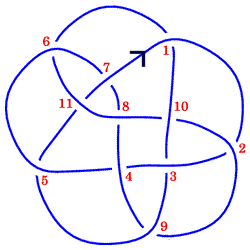
\includegraphics[width=0.90\linewidth]{../data/mixed/gauss_code.png}
        \subcaption{Węzeł o kodzie Gaußa 1 -2 3 -4 5 6 -7 -8 4 -9 2 -10 8 11 -6 -1 10 -3 9 -5 -11 7. Źródło:\\ \url{https://knotinfo.math.indiana.edu/descriptions/gauss_notation.html}.}
    \end{minipage}
    \quad
    \begin{minipage}[b]{.45\linewidth}
        \centering
        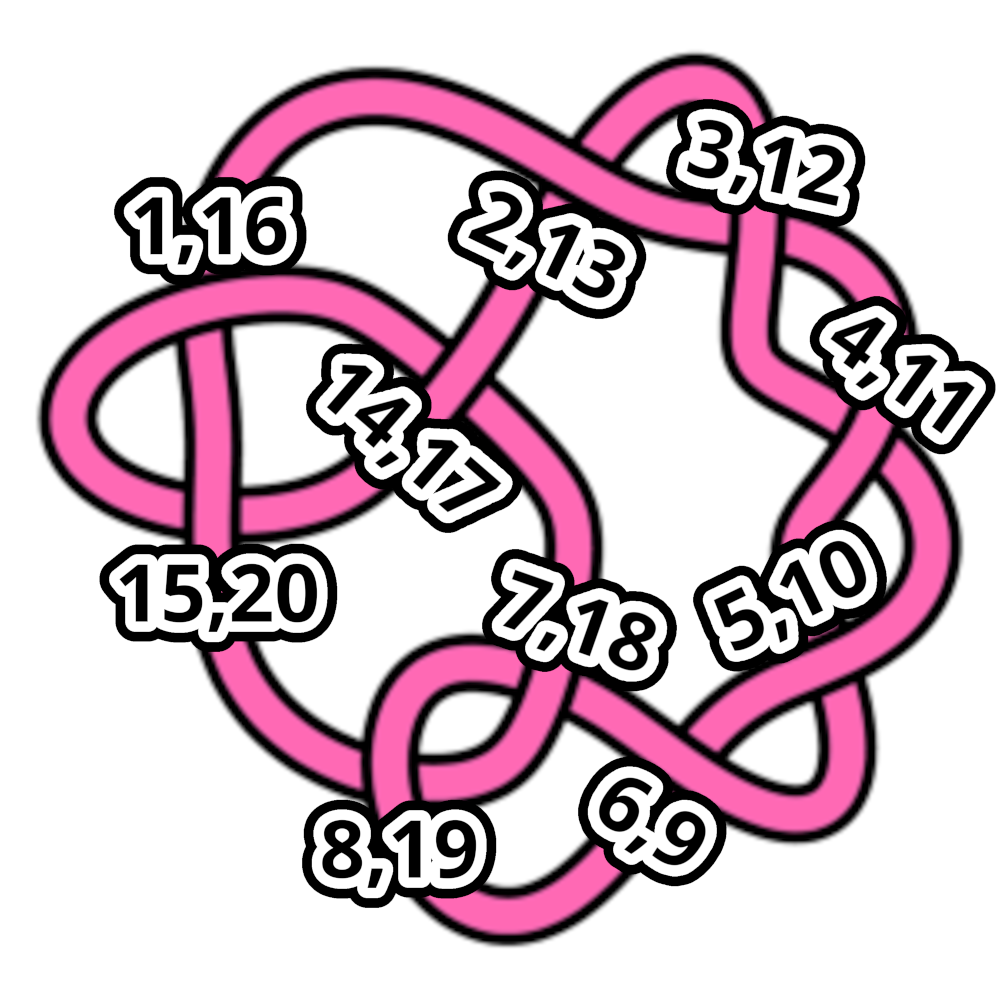
\includegraphics[width=0.90\linewidth]{../data/mixed/dowker_code.png}
        \subcaption{o kodzie (Dowkera-Thistlethwaite'a) 16 18 20 -22 4 2 8 -6 12 10 -14. Źródło:\\ \url{https://knotinfo.math.indiana.edu/descriptions/dt_notation.html}.}
    \end{minipage}
\end{figure}
\end{comment}

W ogólnym przypadku nie można odtworzyć węzła z jego kodu, ale można delikatnie zmienić notację, by było to możliwe.
Kiedy mijamy skrzyżowanie drugi raz, stawiamy minus przed liczbą, jeżeli skrzyżowanie jest lewoskrętne i plus w przeciwnym wypadku.
Nazywa się to rozszerzonym kodem Gaußa.
W naszym przykładzie, rozszerzony kod to 1 -2 3 -4 5 6 -7 -8 \textbf{-4} -9 \textbf{-2} -10 8 11 \textbf{6 -1 -10 3 9 -5 -11 -7}, pogrubione liczby odpowiadają drugim przejściom.

\subsubsection{Notacja Dowkera-Thistlethwaite'a}
\index{notacja!Taita}
\index{notacja!Dowkera-Thistlethwaite'a}
Poprawia nieopisaną tutaj notację Taita, opisana po raz pierwszy w~pracy \cite{dowker83}.

Tak jak w~notacji Gaußa, przemierzamy węzeł zaczynając poza skrzyżowaniem.
Tym razem jednak stare skrzyżowania dostają drugi, nowy numer.
Jak można zauważyć, każde skrzyżowanie ma parzystą oraz nieparzystą etykietę.

\begin{definition}
    Ciąg parzystych liczb występujących na diagramie kolejno przy $1, 3, \ldots$ nazywamy kodem Dowkera-Thistlethwaite'a.
    Jeżeli nieparzysta etykieta odpowiadała podskrzyżowaniu, zapisujemy liczbę z~minusem.
\end{definition}

Opisany powyżej kod nie jest idealny, ponieważ odtworzony z niego węzeł może być lustrzanym odbiciem wyjściowego.
Ogólniej, odbicie dowolnego składnika sumy spójnej nie zmienia kodu całego węzła.
Nie stanowi to jednak dużego problemu, ponieważ notacja została stworzona na potrzeby tablicowania węzłów pierwszych, a~te są niezorientowane.

Zaczynając od zredukowanego diagramu o $n$ skrzyżowaniach nie można doprowadzić do sytuacji, gdzie do pewnego skrzyżowania przypisane są dwie kolejne liczby całkowite.
Dzięki temu problem można przetłumaczyć na język teorii grafów.
Rozpatrzmy graf $G$, którego wierzchołkami są liczby $1, 2, \ldots, 2n$.
Połączmy niesąsiadujące modulo $2n$ wierzchołki o różnej parzystości krawędziami.
Graf ten powstaje przez usunięcie cyklu Hamiltona (łączącego kolejne liczby) z pełnego grafu dwudzielnego.
Zbiór par etykiet przy skrzyżowaniach węzła to skojarzenie doskonałe w grafie $G$.
Liczba skojarzeń prawie pokrywa się z rozwiązaniem zadania znanego w literaturze jako ,,problème des ménages'': na ile sposobów $n$ małżeństw można posadzić przy okrągłym stole tak, by żadne małżeństwo nie siedziało obok siebie i~każdy mężczyzna znalazł się obok dwóch kobiet?
Ustawienia, które powstają przez cykliczne permutowanie należy uznać za tożsame.
Gilbert znalazł w \cite{gilbert56} wzór na $a_n$, liczbę różnych kodów:
\begin{align}
u(m, t) & = 2m \sum_{k=0}^m {2m-k \choose k} \cdot (m-k)! \cdot \frac{(t-1)^k}{2m - k}  \\
a(n) & = \frac{1}{n} \sum_{d\mid n} \left(\frac{n}{d}\right)^d \cdot u \left(d, 1 - \frac{d}{n}\right) \cdot \varphi \left(\frac{n}{d}\right)
\end{align}

Kilka początkowych wartości to $a_3 = 1, 2, 5, 20, 87, 616, 4843, 44128, 444621, \ldots$ (ciąg A002484 w OEIS).

\subsubsection{Notacja Alexandera-Briggsa}
\index{notacja!Alexandera-Briggsa}
W~1927 roku Alexander, Briggs wprowadzili zupełnie inny sposób oznaczania węzłów -- wtedy do 9 skrzyżowań, ale przedłużoną do 10 skrzyżowań przez Rolfsena i używaną po dziś dzień.
Do opisu węzła używa się dwóch liczb: jego indeksu skrzyżowaniowanego z dolnym indeksem, oznaczającym miejsce w tablicy~węzłów.
I~tak węzły o~ośmiu skrzyżowaniach to $8_1, 8_2, \ldots,$ $8_{21}$.
Porządek jest umowny i jego wybór należy do osoby, która jako pierwsza znajdzie wszystkie węzły o danej liczbie skrzyżowań (ale węzeł skręcony występuje zawsze po torusowym).
\index{węzeł!skręcony}%
\index{węzeł!torusowy}%

Od jedenastu skrzyżowań pojawia się mała zmiana: węzły alternujące i niealternujące kataloguje się osobno.
I tak $11n_{185}$ to sto osiemdziesiąty piąty węzeł niealternujący o 11 skrzyżowaniach, zaś $11a_{367}$ to trzysta sześćdziesiąty siódmy alternujący.

Rolfsen w 1976 stworzył z kilkoma błędami tablicę diagramów pierwszych węzłów do 10 skrzyżowań.
Para Perko $10_{161}, 10_{162}$ przedstawia ten sam węzeł, zaś górne skrzyżowanie w~$10_{144}$ powinno być zmienione.
Ostatnie cztery węzły dostały nowe numery, by uniknąć duplikatu.
Kolejną usterką tablicy jest to, że notacja Conwaya oraz wielomian Alexandera dla węzłów $10_{83}$ oraz $10_{86}$ są zamienione miejscami.
Tu czyha pułapka:\footnote{Wiemy o niej dzięki stronie \url{http://stoimenov.net/stoimeno/homepage/ptab/}.} Stojmenow, nowe wydanie książki Rolfsena, atlas węzłów Bar-Natana oraz tablica niezmienników węzłowych Livingstona naprawiają to przez wymianę podpisów.
Podręcznik Kawauchiego wymienia diagramy.

Ze strony internetowej Stojmenowa dowiedzieliśmy się jeszcze czegoś.
Kolejność Rolfsena dla węzłów o 10 skrzyżowaniach obala nomenklaturę Little'a niealternujących oraz nadpisuje numerowanie Taita dla alternujących węzłów.
Alexander, Briggs zrobili wcześniej to samo dla 9 lub mniej skrzyżowań.

\subsubsection{Notacja Conwaya}
\index{notacja!Conwaya}
Wprowadzona przez Conwaya w~pracy \cite{conway70}.
Wymaga znajomości supłów, więc przedstawiamy ją w sekcji supłów: definicji \ref{conway_notation}.

\subsubsection{Nazwy zwyczajowe}
Niektóre węzły i sploty, w szczególności te o niskim indeksie skrzyżowaniowym, występują tak często w teorii węzłów, że doczekały się nazw zwyczajowych.
Oto ich lista:
\begin{compactitem}
% DICTIONARY;unknot;niewęzeł;-
% TODO: nigdzie w książce nie ma definicji niesplotu?
    \item węzeł $0_1$ to niewęzeł;
% DICTIONARY;trefoil knot;trójlistnik;-
    \item węzeł $3_1$ to trójlistnik,
% DICTIONARY;figure-eight;ósemka;-
    \item węzeł $4_1$ to ósemka albo węzeł Listinga,
% DICTIONARY;cinquefoil knot;pięciolistnik;-
    \item węzeł $5_1$ to pięciolistnik albo węzeł Solomona (!),
% DICTIONARY;stevedore knot;węzeł dokerski;-
    \item węzeł $6_1$ to węzeł dokerski,
    \item węzeł 11n34 to węzeł Conwaya,
    \item węzeł 11n42 to węzeł Kinoshity-Terasakiego,
    \item węzeł 12n242, czyli $(-2, 3, 7)$-precel, to węzeł Fintushela-Sterna,
% DICTIONARY;granny knot;węzeł babski;-
    \item suma spójna takich samych trójlistników to węzeł babski,
% DICTIONARY;square knot;węzeł prosty/płaski
    \item suma spójna lustrzanych trójlistników to węzeł prosty albo płaski (dość niefortunna nazwa),
    \item splot $2_1^2$ (L2a1) to splot Hopfa,
    \item splot $4_1^2$ (L4a1) to węzeł Solomona (!),
    \item splot $5_1^2$ (L5a1) to splot Whiteheada,
    \item splot $6_2^3$ (L6a4) to pierścienie Boromeuszy.
\end{compactitem}


\chapter{W stronę węzłów pierwszych}
\section{Operacje na węzłach}
Mając dany diagram splotu zorientowanego, można odwrócić jego wszystkie ogniwa albo wszystkie skrzyżowania.
Działania te nazywamy odpowiednio rewersem i~lustrem, opisujemy je w~pierwszej podsekcji.
Dalej pojawi się suma niespójna oraz spójna, odpowiednik mnożenia liczb naturalnych zbadany dokładniej przez Schuberta około 1954 roku.
\index[persons]{Schubert, Horst}%
Znacznie później (bo dopiero w~sekcji \ref{sec:tangle}) wprowadzimy jeszcze sumę i~iloczyn supłów.


\subsection{Lustro i~rewers. Węzły skrętne i zwierciadlane}
\begin{definition}[lustro]
% DICTIONARY;mirror;lustro/lustrzany;węzeł
\index{lustro}%
\index{węzeł!lustrzany}% TODO: to się może mylić ze zwieciadlanym
    Niech $L$ będzie zorientowanym splotem.
    Splot $mL$ powstały przez odbicie splotu $L$ względem dowolnej płaszczyzny nazywamy lustrem.
\end{definition}

\begin{definition}[rewers]
% DICTIONARY;reverse;rewers/odwrotny;węzeł
\index{rewers}%
\index{węzeł!odwrotny}%
    Niech $L$ będzie zorientowanym splotem.
    Splot $rL$ powstały przez odwrócenie orientacji wszystkich ogniw splotu $L$ nazywamy rewersem.
\end{definition}

\begin{comment}
\begin{figure}[H]
    \begin{minipage}[b]{.32\linewidth}
        \centering
        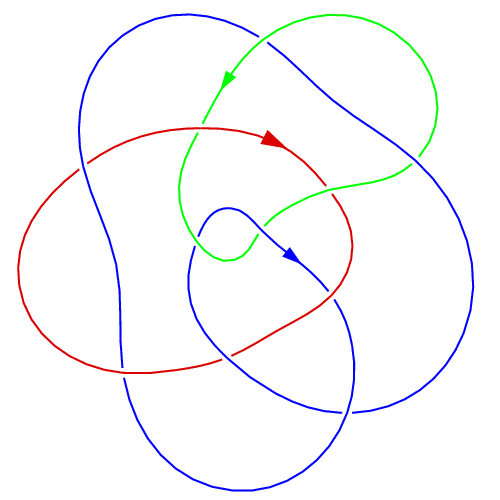
\includegraphics[width=\linewidth]{../data/link_mirror.png}
        \subcaption{lustro $mL$}
    \end{minipage}
    \begin{minipage}[b]{.32\linewidth}
        \centering
        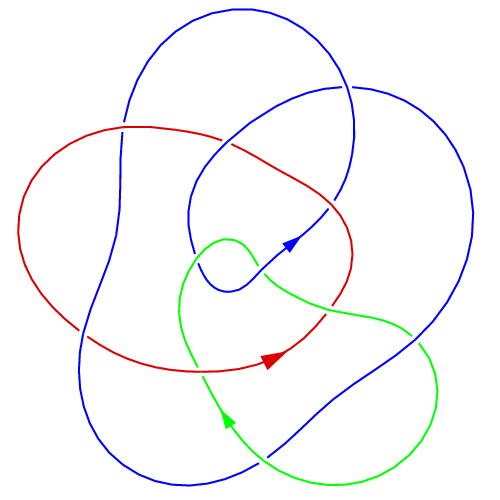
\includegraphics[width=\linewidth]{../data/link.png}
        \subcaption{przykładowy splot $L$}
    \end{minipage}
    \begin{minipage}[b]{.32\linewidth}
        \centering
        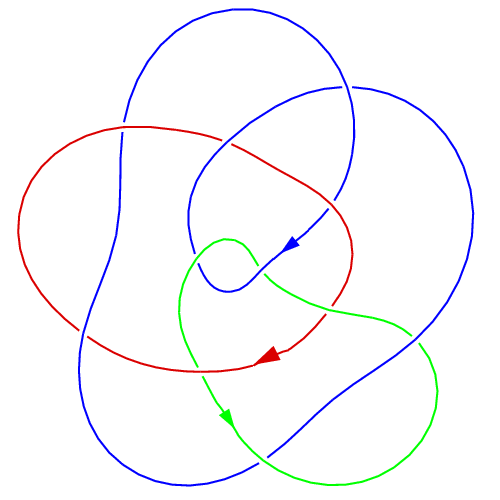
\includegraphics[width=\linewidth]{../data/link_reverse.png}
        \subcaption{rewers $rL$}
    \end{minipage}
\end{figure}
\end{comment}

Na lewym obrazku odbiliśmy diagram względem poziomej prostej, innym sposobem na otrzymanie lustra jest odwrócenie wszystkich skrzyżowań, co odpowiada odbijaniu względem płaszczyzny papieru.
Zauważmy, że wykonując powyższe operacje na węźle możemy otrzymać mniej niż czterech różne obiekty ($L$, $mL$, $rL$, $mrL$) -- na przykład trójlistnik jest własnym rewersem, ale nie lustrem.

Wyróżniamy pięć typów symetrii węzłów:

% DICTIONARY;chiral;skrętny/chiralny;węzeł
\begin{definition}[całkowicie chiralny albo skrętny]
\index{węzeł!chiralny}%
\index{węzeł!skrętny|see {węzeł lustrzany}}%
    Węzły $K$, $rK$, $mK$ są parami nierównoważne. % chiral 9_32
\end{definition}

% DICTIONARY;reversible;odwracalny;węzeł
\begin{definition}[odwracalny]
    \index{węzeł!odwracalny}%
    Węzły $K \cong rK$ są równoważne. % reversible 3_1
\end{definition}

% DICTIONARY;achiral/amphicheiral;zwierciadlany;węzeł
\begin{definition}[zwierciadlany ujemnie]
    \index{węzeł!zwierciadlany}%
    Węzły $K \cong mrK$ są równoważne. % negative amphicheiral 8_17
\end{definition}

\begin{definition}[zwierciadlany dodatnio]
    Węzły $K \cong mK$ są równoważne. % positive amphicheiral 12a_427
\end{definition}

\begin{definition}[całkowicie zwierciadlany]
    Węzły $K, rK, mK$ są parami równoważne. % fully amphicheiral 4_1
\end{definition}

\begin{example}
    Węzeł $9_{32}$ jest całkowicie skrętny.
\end{example}

% Całkowicie skrętne są też między innymi wszystkie węzły torusowe.
% TODO: wiki pisze Each nontrivial torus knot is prime[4] and chiral.[2]

\begin{example}
    \label{exm:trefoil_is_chiral}
    Trójlistnik jest odwracalny, ale nie zwierciadlany.
\end{example}

Po raz pierwszy odkrył to Max Dehn w 1914 roku \cite{dehn14}.
Oto, jak tego dokonał.
% równik = equator
% równoleżnik = parallel (of latitude), najdłuższy równoleżnik to równik
% południk = meridian (of longitude)
% https://math.stackexchange.com/questions/2511364/how-did-dehn-prove-that-the-trefoil-is-chiral myli te pojęcia: pisze o meridian i longitude, kiedy oryginalna praca Dehna operowała na longitude i latitude
Iloraz grafu Cayleya dla grupy podstawowej trójlistnika, $G = \pi_1(S^3 - K)$, zanurza się w~produkt $\mathbb H^2 \times \R$, co pozwala wyznaczyć grupę zewnętrznych automorfizmów grupy $G$, $\Z/2\Z$.
\index{grupa!podstawowa}
% DICTIONARY;latitude;szerokość geograficzna;geografia
% DICTIONARY;longitude;długość geograficzna;geografia
% DICTIONARY;meridian (of longitude);południk;geografia
% DICTIONARY;parallel (of latitude);równoleżnik;geografia
% DICTIONARY;---;geografia;-
Korzystając z~południków i~równoleżników pokazał następnie, że nietrywialny automorfizm zewnętrzny odwraca orientację przestrzeni otaczającej.

My przekonamy się o~tym po wyznaczeniu wielomianu Jonesa trójlistnika, patrz wniosek \ref{cor:joines_of_amphicheiral}.

\begin{example}
    Węzeł $8_{17}$ jest zwierciadlany ujemnie, ale nie odwracalny.
\end{example}

Sześćdziesiąt lat temu matematycy nie byli pewni, czy węzły nieodwracalne w~ogóle istnieją \cite[problem 10]{fox62};
obecnie wiadomo, że nieodwracalne są prawie wszystkie węzły (Murasugi \cite[s.~46]{murasugi96}).
\index[persons]{Murasugi, Kunio}%
W~roku 1962 Ralph Fox wskazał kilku kandydatów do tego tytułu.
\index[persons]{Fox, Ralph}%
Hale Trotter odkrył rok później nieskończoną rodzinę nieodwracalnych precli, patrz \ref{prp:pretzel_not_invertible}.
\index[persons]{Trotter, Hale}%

% MAKOTO SAKUMA - A SURVEY OF THE IMPACT OF THURSTON’S WORK ON KNOT THEORY
% Hartley [129] realized that one can apply this method to the problem of identifying noninvertible knots, as follows. Suppose no automorphism of Γ maps γ to γ−1. Then the set R(G(K), Γ, γ) is possibly different from the set R(G(K), Γ, γ−1), and there is a chance to show noninvertibility of K by comparing the homology invariants associated with φ ∈ R(G(K), Γ, γ) with those associated with φ′ ∈ R(G(K), Γ, γ−1). Hartley showed that this method is quite effective: he completely determined the 36 non-invertible knots up to 10 crossings claimed by Conway to be noninvertible.

\begin{example}
    Węzeł $12a_{427}$ jest zwierciadlany dodatnio, ale nie odwracalny.
\end{example}

Żaden inny węzeł pierwszy o mniej niż 13 skrzyżowaniach nie ma tej cechy.

\begin{example}
\label{property_of_eight_knot}%
    Ósemka $4_1$ jest całkowicie zwierciadlana.
\end{example}

To najprostszy typ symetrii, wystarczy jawnie wskazać przekształcenie między diagramem węzła, jego lustra oraz odwrotności.

Tait odnosił wrażenie, że zwierciadlane węzły mają parzysty indeks skrzyżowań, ale Hoste, Thistlethwaite znaleźli w~1998 kontrprzykład o~piętnastu skrzyżowaniach, $15_{700}$. % wg https://mathworld.wolfram.com/AmphichiralKnot.html
(Czwarta) hipoteza Taita jest prawdziwa dla węzłów pierwszych, alternujących.

\begin{proposition}[10.4.4 w \cite{kawauchi96}, \ref{cor:joines_of_amphicheiral} u nas]
    Niech $K$ będzie węzłem zwierciadlanym.
    Wtedy
    \begin{align}
        V(t) & = V(1/t) \\
        P(a, z) & = P(1/a, z) \\
        F(a, z) & = F(1/a, z),
    \end{align}
    gdzie $\jones, P, F$ oznacza kolejno wielomian Jonesa, HOMFLY oraz Kauffmana.
    Równość $\conway(z) = \conway(-z)$ zachodzi dla wszystkich węzłów, zwierciadlanych lub nie.
\end{proposition}

Poniższa tabela oparta jest (kolejno) o~ciągi
\href{https://oeis.org/A051766}{51766},
\href{https://oeis.org/A051769}{51769},
\href{https://oeis.org/A051768}{51768},
\href{https://oeis.org/A051767}{51767},
\href{https://oeis.org/A052400}{52400},
z bazy danych ``The On-Line Encyclopedia of Integer Sequences'' (OEIS).

\begin{table}[h]
    \centering
    \begin{tabular}{@{}*{20}l@{}} \toprule
        skrzyżowania & 3 & 4 & 5 & 6 & 7 & 8 & 9 & 10 & 11 & 12 & 13 & 14 \\ \midrule
        całkowicie skrętne & 0 & 0 & 0 & 0 & 0 & 0 & 2 & 27 & 187 & 1103 & 6919 & 37885 \\
        odwracalne & 1 & 0 & 2 & 2 & 7 & 16 & 47 & 125 & 365 & 1015 & 3069 & 8813 \\
        $-$ zwierciadlane & 0 & 0 & 0 & 0 & 0 & 1 & 0 & 6 & 0 & 40 & 0 & 227 \\
        $+$ zwierciadlane & 0 & 0 & 0 & 0 & 0 & 0 & 0 & 0 & 0 & 1 & 0 & 6 \\
        zwierciadlane & 0 & 1 & 0 & 1 & 0 & 4 & 0 & 7 & 0 & 17 & 0 & 41 \\
        \bottomrule
        \hline
    \end{tabular}
    \caption{Liczba węzłów o~poszczególnych typach symetrii}
\end{table}

\begin{definition}[10.3.2 w \cite{kawauchi96}]
    Niech $K \subseteq S^3$ będzie węzłem.
    Jeśli istnieje inwolucja pary $(S^3, K)$, która zachowuje orientację sfery, ale odwraca orientację węzła, to węzeł $K$ nazywamy silnie odwracalnym.
\end{definition}

\begin{proposition}
    Jeśli węzeł jest silnie odwracalny, to jest też odwracalny.
    Implikacja odwrotna nie zachodzi.
\end{proposition}

Hipotezę, że implikacja odwrotna jednak zachodzi, postawił Montesinos \cite[problem 1.6]{kirby78}, on też zdefiniował klasę silnie odwracalnych węzłów \cite{montesinos75}.
\index[persons]{Montesinos, José}%

\begin{proof}
\index[persons]{Hartley, Richard}%
\index[persons]{Whitten, Wilbur}%
    Pierwsza część jest oczywista.
    Hartley \cite{hartley80} oraz Whitten \cite{whitten81} niezależnie od siebie zaproponowali kontrprzykłady do implikacji odwrotnej.
\end{proof}

Ale hiperboliczny węzeł odwracalny jest silnie odwracalny.
% Kawauchi bez dowodu.

\begin{proposition}
    Każdy wielomian Alexandera jest realizowany przez pewien silnie odwracalny węzeł.
\end{proposition}

\begin{proof}
\index[persons]{Sakai, Tsuyoshi}%
    Sakai konstruuje w \cite{sakai83} silnie odwracalny węzeł o dowolnie wybranym cyklicznym module Alexandera.
\end{proof}

% Koniec podsekcji Lustro i rewers




\subsection{Węzły okresowe}
\index{węzeł!okresowy|(}%
Można wyróżnić jeszcze jeden rodzaj symetrii.

% DICTIONARY;period;okres;-
% DICTIONARY;periodic;okresowy;węzeł
\begin{definition}
\label{def:period}%
    Węzeł $K$ nazywamy $n$-okresowym, jeśli istnieje obrót $f \colon \R^3 \to \R^3$ o~kąt $2\pi/n$ wokół pewnej prostej $l$, rozłącznej z~węzłem, taki że $f(K) = K$.
\end{definition}

Zamiast obrotów można rozpatrywać dowolne odwzorowania okresowe $f \colon S^3 \to S^3$, których zbiór punktów stałych jest rozłączny z węzłem $K$, homeomorficzny z $S^1$ oraz które trzymają węzeł $K$ w miejscu, ale dostaje się wtedy dokładnie taką samą klasę węzłów.
\index{hipoteza!Smitha}
Wynika to z hipotezy Smitha, otrzymanej z połączenia głębokich teorii dotyczących geometrii i topologii 3-rozmaitości.
% Kawauchi, ćwiczenie 10.1.10
% Morgan-Bass 1984

\begin{proposition}
    Zbiór wszystkich okresów jest niezmiennikiem węzłów.
\end{proposition}

Nieodwracalny węzeł $8_{17}$ nie posiada żadnych okresów.
% ćwiczenie 10.1.5 w Kawauchi
Węzeł $5_1$ 5-okresowy, co widać na standardowym diagramie, oraz 2-okresowy, tę drugą symetrię można dostrzec na diagramie realizującym indeks mostowy.
Trójlistnik ma dokładnie dwa okresy, $2$ i~$3$.
Ogólniej, jak głosi Kawauchi \cite[ćwiczenie 10.1.9]{kawauchi96}:

\begin{proposition}
    Jedynymi okresami węzła $(p, q)$-torusowego są dzielniki liczb $p$ oraz $q$.
\end{proposition}

Z~każdym węzłem okresowym związany jest inny, prostszy węzeł.
Niech $f$ będzie obrotem z definicji \ref{def:period}, zaś $p \colon \R^3 \to \R^3/f \simeq \R^3$ rzutem na przestrzeń ilorazową.
% DICTIONARY;quotient;ilorazowy;węzeł
\index{węzeł!ilorazowy}%
Wtedy $p(K)$ nazywamy \emph{węzłem ilorazowym}, zaś $K$ to jego $n$-krotne nakrycie.

Murasugi podał dwa warunki, które musi spełniać węzeł o~okresie $n = p^r$, gdzie $r$ jest liczbą pierwszą.
Do ich zrozumienia potrzebujemy prostej definicji.
Ustalmy półprostą, która nie jest styczna do węzła $K$, po czym zorientujmy ją oraz węzeł.
Indeksem zaczepienia $\lambda$ węzła $p(K)$ jest różnica między liczbą skrzyżowań dodatnich oraz ujemnych wzdłuż półprostej (bez znaku).

\begin{proposition}[warunek Murasugiego]
\index{warunek Murasugiego}%
\label{prp:murasugi_periodic}%
    Niech $K$ będzie węzłem o~okresie $n = p^r$, gdzie $p$ jest liczbą pierwszą.
    Niech $J$ będzie jego węzłem ilorazowym, z~indeksem zaczepienia $\lambda$.
    Wtedy wielomian $\alexander_J$ jest dzielnikiem wielomianu $\alexander_K$ oraz istnieje pewna całkowita liczba $k$, taka że
    \begin{equation}
        \alexander_K(t) \equiv \pm t^k \alexander_J(n)^n \left(1 + t + t^2 + \ldots + t^{\lambda - 1}\right)^{n-1} \mod p.
    \end{equation}
\end{proposition}

\begin{proof}
    Mozolne operacje na macierzach, których wyznacznikiem jest wielomian Alexandera, patrz \cite{murasugi71}.
    Kawauchi przedstawia inny dowód: najpierw dowodzi tego dla węzła torusowego $T_{n, d}$, którego węzłem ilorazowym jest niewęzeł.
    W ogólnym przypadku, korzysta z relacji kłębiastej dla wielomianu Conwaya.
    Szczegóły oraz odsyłacze do dalszych prac znaleźć można w jego przeglądowej publikacji \cite[s. 122-124]{kawauchi96}.
\end{proof}

\index{węzeł!okresowy|(}%

% koniec podsekcji Węzły okresowe




\subsection{Suma niespójna i~suma spójna}

\begin{definition}[suma niespójna]
% DICTIONARY;distant union;suma niespójna;-
\index{suma niespójna}%
    Niech $L_1$ oraz $L_2$ będą splotami, które leżą po różnych stronach ustalonej płaszczyzny w przestrzeni $\R^3$.
    Teoriomnogościową sumę $L_1 \sqcup L_2$ nazywamy sumą niespójną splotów.
\end{definition}

\begin{definition}[suma spójna]
% DICTIONARY;connected sum;suma spójna;-
\index{suma spójna}%
    Niech $K_1, K_2$ będą zorientowanymi węzłami.
    Natnijmy każdy z nich w dwóch punktach tego samego krótkiego łuku, a następnie zszyjmy dwoma łukami, które nie przecinają już istniejących, jak na obrazku.
    Otrzymany węzeł nazywamy sumą spójną węzłów $K_1$ oraz $K_2$ i oznaczamy przez $K_1 \shrap K_2$.
\begin{comment}
    \[
        \begin{tikzpicture}[baseline=-0.65ex,scale=0.09]
        \useasboundingbox (-12, -15) rectangle (12, 10);
        \begin{knot}[clip width=5, flip crossing/.list={5}, ignore endpoint intersections=false,]
            \strand[thick] (-3.5, -3.5) [in=down, out=up] to (3.5, 3.5);
            \strand[thick] (3.5, 3.5) [in=right, out=up] to (-4.5, 10);
            \strand[thick] (-4.5, 10) [in=up, out=left] to (-10, 3.5);
            \strand[thick] (-10, 3.5) to (-10, -3.5);
            \strand[thick] (-10, -3.5) [in=left, out=down] to (-4.5, -10);
            \strand[thick] (-4.5, -10) [in=down, out=right] to (3.5, -3.5);
            \strand[thick] (3.5, -3.5) [in=down, out=up] to (-3.5, 3.5);
            \strand[thick] (-3.5, 3.5) [in=left, out=up] to (4.5, 10);
            \strand[thick] (4.5, 10) [in=up, out=right] to (10, 3.5);
            \strand[thick, -Latex] (10, 3.5) to (10, -3.5);
            \strand[thick] (10, -3.5) [in=right, out=down] to (4.5, -10);
            \strand[thick] (4.5, -10) [in=down, out=left] to (-3.5, -3.5);
            \node at (0, -15) {$K_1$};
        \end{knot}
        \end{tikzpicture}
        \shrap
        \begin{tikzpicture}[baseline=-0.65ex,scale=0.09]
        \useasboundingbox (-12, -15) rectangle (12, 10);
        \begin{knot}[clip width=5, flip crossing/.list={6}, ignore endpoint intersections=false,]
            \strand[thick] (-3.5, -3.5) [in=down, out=up] to (3.5, 3.5);
            %\strand[thick] (3.5, 3.5) [in=right, out=up] to (-4.5, 10);
            %\strand[thick] (-4.5, 10) [in=up, out=left] to (-10, 3.5);
            \strand[thick] (-10, -3.5) [in=left, out=up] to (0, 6.5);
            \strand[thick, Latex-] (-10, -3.5) [in=left, out=down] to (-4.5, -10);
            \strand[thick] (-4.5, -10) [in=down, out=right] to (3.5, -3.5);
            \strand[thick] (3.5, -3.5) [in=down, out=up] to (-3.5, 3.5);
            %\strand[thick] (-3.5, 3.5) [in=left, out=up] to (4.5, 10);
            %\strand[thick] (4.5, 10) [in=up, out=right] to (10, 3.5);
            \strand[thick] (10, -3.5) [in=right, out=up] to (0, 6.5);
            \strand[thick] (10, -3.5) [in=right, out=down] to (4.5, -10);
            \strand[thick] (4.5, -10) [in=down, out=left] to (-3.5, -3.5);
            %
            \strand[thick] (-3.5, 3.5) [in=left, out=up] to (0, 10);
            \strand[thick] (3.5, 3.5) [in=right, out=up] to (0, 10);
            \node at (0, -15) {$K_2$};
        \end{knot}
        \end{tikzpicture}
        =
        \begin{tikzpicture}[baseline=-0.65ex,scale=0.09]
        \useasboundingbox (-27, -15) rectangle (27, 10);
        \begin{knot}[clip width=5, flip crossing/.list={5, 22, 23}, ignore endpoint intersections=false,]
            \strand[thick] (-18.5, -3.5) [in=down, out=up] to (-11.5, 3.5);
            \strand[thick] (-11.5, 3.5) [in=right, out=up] to (-19.5, 10);
            \strand[thick] (-19.5, 10) [in=up, out=left] to (-25, 3.5);
            \strand[thick] (-25, 3.5) to (-25, -3.5);
            \strand[thick] (-25, -3.5) [in=left, out=down] to (-19.5, -10);
            \strand[thick] (-19.5, -10) [in=down, out=right] to (-11.5, -3.5);
            \strand[thick] (-11.5, -3.5) [in=down, out=up] to (-18.5, 3.5);
            \strand[thick] (-18.5, 3.5) [in=left, out=up] to (-10.5, 10);
            \strand[thick] (-10.5, 10) [in=left, out=right] to (-5, 2);
            \strand[thick, -Latex] (-5, 2) to (-5+6, 2);
            \strand[thick] (5, 2) to (-5+6, 2);
            \strand[thick] (3, -2) to [in=left, out=right] (10.5, -10);
            \strand[thick, -Latex] (3, -2) to (-3, -2);
            \strand[thick] (-5, -2) to (-3, -2);
            \strand[thick] (-5, -2) [in=right, out=left] to (-10.5, -10);
            \strand[thick] (-10.5, -10) [in=down, out=left] to (-18.5, -3.5);
            %%%
            \strand[thick] (11.5, -3.5) [in=down, out=up] to (18.5, 3.5);
            \strand[thick] (-10 +15, 2) [in=left, out=right] to (15, 6.5);
            \strand[thick] (10.5, -10) [in=down, out=right] to (18.5, -3.5);
            \strand[thick] (18.5, -3.5) [in=down, out=up] to (11.5, 3.5);
            \strand[thick] (25, -3.5) [in=right, out=up] to (15, 6.5);
            \strand[thick] (25, -3.5) [in=right, out=down] to (19.5, -10);
            \strand[thick] (19.5, -10) [in=down, out=left] to (11.5, -3.5);
            \strand[thick] (11.5, 3.5) [in=left, out=up] to (15, 10);
            \strand[thick] (18.5, 3.5) [in=right, out=up] to (15, 10);
            %%%
            \node at (0, -15) {$K_1 \shrap K_2$};
        \end{knot}
        \end{tikzpicture}
    \]
\end{comment}
\end{definition}

Pojęcie sumy spójnej węzłów (oraz satelity, opisane później) wprowadził do matematyki Schubert w \cite{schubert49}.
\index[persons]{Schubert, Horst}%

Ważna jest orientacja składników: suma dwóch trójlistników może być węzłem babskim lub prostym\footnote{To jedno z niewielu miejsc, gdzie nomenklatura pochodzi od żeglarzy.}.
\label{two_sums_of_two_trefoils}%
Uzasadnienie, że te węzły są różne, nie jest łatwym zadaniem.
Fox twierdzi, że Seifert wiedział to już w~1933 roku.
% Seifert, Herbert - Verschlingungsinvarianten. (German) Zbl 0008.18101 Sitzungsber. Preuß. Akad. Wiss., Phys.-Math. Kl. 1933, No. 26-29, 811-828 (1933).
Pokazał też w~króciutkim artykule \cite{fox52}, że

\begin{proposition}
    Dopełnienia węzła babskiego oraz prostego nie są homeomorficzne.
\end{proposition}

Suma tak samo skręconych trójlistników ma niezerową sygnaturę, więc nie może być plastrowa.
Natomiast suma przeciwnie skręconych jest plastrowa.\footnote{Nie wiem, skąd to wiem.}
\index{węzeł!plastrowy}

Warunku, by zszywające łuki nie przecinały diagramów, nie można pominąć: Cromwell w~\cite[s. 90]{cromwell04} pokazuje przykład dwóch niewęzłów, z~których otrzymano niepoprawnie dwie różne sumy, $6_1$ oraz $8_{20}$.

W topologii rozważa się podobną operację dla $n$-rozmaitości: z~każdej z~nich wycina się kulę, po czym skleja wzdłuż brzegowej sfery w~jedną rozmaitość.
Ale kiedy zajmujemy się węzłami, nie interesuje nas struktura rozmaitości (gdyż każdy węzeł jest homeomorficzny z~okręgiem), tylko zanurzenie w otaczającą przestrzeń.

\begin{proposition}
    Suma spójna węzłów jest dobrze określonym działaniem.
\end{proposition}

Suma spójna nie jest dobrze określona dla splotów: nie istnieje kanoniczny wybór, które ogniwa łączyć ze sobą.

\begin{proof}
    Niech dane będą węzły $K_1$ oraz $K_2$ oraz dwa różne łuki $\gamma_1$, $\gamma_2$, których można użyć do konstrukcji sumy spójnej.
    Skurczmy $K_1$ tak, by był bardzo mały, przeciągnijmy najpierw przez łuk $\gamma_1$, a~następnie wzdłuż węzła $K_2$ do miejsca, gdzie zaczyna się łuk $\gamma_2$.
    Na koniec odwróćmy proces, z łukiem~$\gamma_2$ w~miejscu łuku $\gamma_1$.
\end{proof}

\begin{proposition}
    Suma spójna jest działaniem łącznym oraz przemiennym.
    Niewęzeł stanowi jej element neutralny.
\end{proposition}

Prosty dowód tego faktu pozostawiamy Czytelnikowi.
W języku algebry mówimy, że węzły z~sumą spójną tworzą półgrupę (tak jak liczby naturalne z działaniem dodawania).
Dużo później pokażemy, że działaniu $\shrap$ brakuje elementów przeciwnych, więc ta struktura algebraiczna nie jest grupą.

\begin{proposition}
\label{first_time_sum_is_trivial}%
    Niech $K_1, K_2$ będą takimi węzłami, że $K_1 \shrap K_2 = \SmallUnknot$. Wtedy $K_1 = K_2 = \SmallUnknot$.
\end{proposition}

\begin{proof}[Niedowód]
% DICTIONARY;Mazur swindle;szwindel Mazura;-
    Technika ta zwana jest szwindlem Mazura.
\index{szwindel Mazura}%
    Załóżmy, że $K \shrap L = \SmallUnknot$ i~dopuśćmy wyjątkowo węzły dzikie.
    Skonstruujmy sumę $K \shrap L \shrap K \shrap \ldots$,
    przy czym kolejne składniki powinny zmniejszać się,
    aby ich suma nadal była węzłem.
    Wtedy
    \begin{align*}
        K & \simeq K \shrap [(L \shrap K) \shrap (L \shrap K) \ldots] \\
         & \simeq (K \shrap L) \shrap (K \shrap L) \shrap \ldots
         \simeq \SmallUnknot \shrap \SmallUnknot \shrap \ldots
         \simeq \SmallUnknot.
    \end{align*}
    Analogicznie pokazujemy, że $L \simeq \SmallUnknot$.
    (To jedyne miejsce w~całej książce, gdzie użyte zostają węzły dzikie.)
\end{proof}

W poprzednim wydaniu książki znajdowała się informacja, że dla dowodu tego faktu trzeba przytoczyć narzędzia topologii algebraicznej: powierzchnie Seiferta i~genus; wtedy jest to bezpośredni wniosek z~faktów \ref{prp:genus_detects_unknot} oraz \ref{prp:genus_of_sum}.
O~tym samym dowodzie wspomina Kawauchi \cite[s. 33]{kawauchi96}, a~fakt nazywa twierdzeniem o~nieanulowaniu.
Okazuje się jednak, że elementarny dowód istnieje!
% odkryte w https://aperiodical.com/2018/07/the-big-internet-math-off-round-1-jim-propp-v-zoe-griffiths/

Trzeba zajrzeć do \cite[s. 18-20]{kauffman95} dla dwóch rysunków tamże.

\begin{proof}
    (Na podstawie \cite[s. 18-20]{kauffman95}).
    Wyobraźmy sobie, że węzeł oraz torus połykająco-podążający $T$ został zawieszony między dwiema ścianami pokoju i~załóżmy nie wprost, że suma $K = K_1 \shrap K_2$ jest trywialna.
    Wtedy pewien homeomorfizm pokoju, który nie rusza ścian, prostuje sumę (zamienia pozornie zaplątany węzeł $K$ w odcinek $L$). 

    Niech $\pi$ będzie dowolną płaszczyzną zawierającą wyprostowaną sumę $K$.
    Tnie część wspólną torusa $T$ oraz ścian w czterech punktach, oznaczmy je $A, B$ (na lewej ścianie) oraz $C, D$ (na prawej).
    Zauważmy, że $\pi$ tnie $T$ w łukach, które wychodzą z $A, B, C, D$ oraz pewnych zamkniętych krzywych.
    Łuk wychodzący z~punktu $A$ nie może łączyć go z punktami $B$ lub $D$, ponieważ te leżą po drugiej stronie odcinka $L$ na płaszczyźnie $\pi$.
    
    Łuk $AC$ przedstawia niewęzeł.
    Jednocześnie jest on obrazem pewnego łuku, który łączył końce torusa $T$, zatem musi być równoważny z~węzłem-towarzyszem.
\end{proof}

Półgrupę węzłów z~operacją sumy spójnej można uczynić grupą na dwa sposoby: albo zmieniając działanie, albo osłabiając równoważność węzłów.
Drugi pomysł jest lepszy niż pierwszy.
Na początku lat pięćdziesiątych Milnor wprowadził pojęcie zgodności.
\index{węzeł!plastrowy}%
\index{węzeł!zgodny}%
Element neutralny nowej grupy to węzły plastrowe, ich opis leży w~sekcji \ref{sec:slice}.
Zgodność i plastrowe węzły to zagadnienia zakorzenione w~czterowymiarowej topologii.

Kawauchi \cite[s. 50-53]{kawauchi96} opisuje $2n$-sumę Murasugiego tak, że $2$-suma to nasza suma spójna, zaś $4$-suma to ,,plumbing'' (coś, czego nie znamy) i dodaje komentarz, że jest bardzo przydatna do badania powierzchni Seiferta czy genusu.
\index{suma Murasugiego}%
Została wprowadzona dawno temu w~\cite{murasugi58}, by szacować stopień wielomianu Alexandera alternujących węzłów.
\index[persons]{Murasugi, Kunio}%

% DICTIONARY;suma paskowa;band sum;-
Innym uogólnieniem jest suma paskowa, patrz \cite[s. 31-32, 43]{kawauchi96}, specjalny przypadek hiperbolicznej transformacji splotu oraz fuzji splotu.
% TODO: sprawdzić, czy fuzja splotu ma trafić do indeksu

% Koniec podsekcji Suma niespójna i suma spójna





% DICTIONARY;prime;pierwszy;węzeł
% DICTIONARY;composite;złożony;węzeł
\section{Węzły pierwsze}
\index{węzeł!pierwszy|(}%
Suma spójna jest dla węzłów tym, czym mnożenie dla liczb naturalnych.
Analogia ta nabiera sensu, gdy zdefiniujemy węzły pierwsze, odpowiedniki liczb pierwszych.
Do ich dobrego zrozumienia warto znać powierzchnie Seiferta (ale przy pierwszym czytaniu nie trzeba).

\begin{definition}[węzeł pierwszy]
\label{def:prime_knot}%
    Niech $K$ będzie węzłem różnym od niewęzła.
    Jeśli nie przedstawia się jako suma spójna $K_1 \shrap K_2$
    dwóch nietrywialnych węzłów $K_1, K_2$, nazywamy go węzłem pierwszym.
    W~przeciwnym razie mówimy, że jest złożony.
\end{definition}

Pokażemy później, że rozkład na węzły pierwsze istnieje i~wspomnimy, dlaczego jest jedyny.
Fakt \ref{prp:genus_of_sum} stanowi odpowiednik zasadniczego twierdzenia arytmetyki (i jest od niego trochę trudniejszy w~dowodzie).
Każdy węzeł jest sumą spójną siebie oraz niewęzła, dlatego byłoby miło, gdyby niewęzeł nie dał się zapisać jako suma dwóch innych węzłów.
Jest to dokładnie wniosek \ref{cor:connected_sum_no_inverses}: suma spójna nie posiada elementów odwrotnych.

% TODO: jak przedłużyć mimo niejednoznaczności na złożone?

Przesmyk to wąskie skrzyżowanie między dwiema rozłącznymi częśćmi diagramu.
\index{przesmyk}

\begin{proposition}
\index{splot!rozszczepialny}%
    Niech $L$ będzie alternującym splotem bez przesmyków.
    Jeśli diagram splotu $L$ jest spójny, to splot jest nierozszczepialny.
    Jeśli splot nie jest rozszczepialny, to jest też pierwszy jeśli dla każdego okręgu przecinającego diagram w dwóch niepodwójnych punktach, przekrój wnętrza okręgu z~diagramem jest łukiem.
\end{proposition}

Innymi słowy, jeśli alternujący splot jest złożony, widać to bezpośrednio na każdym jego alternującym diagramie.
Jako pierwszy pokazał to Menasco w~\cite{menasco84}.
Jego dowód opiera się na multiplikatywności wielomianu BLM/Ho.
\index{wielomian!BLM/Ho}

Czy węzłów pierwszych jest nieskończenie wiele?
Tak, patrz fakt \ref{prp:infinitely_many_prime_knots}, potrafimy nawet oszacować liczbę $K_n$ węzłów pierwszych oraz $L_n$ splotów pierwszych.
W roku 1987 C. Ernst, D. Sumners w~oparciu o~wyniki Thistlethwaite'a, Kauffmana, oraz Murasugiego dotyczące węzłów alternujących pokazali w~\cite{ernst87}, że $K_n \ge \frac 1 3 (2^{n- 2} - 1)$, przy czym węzły lustrzane traktowane są jako różne.
% te wyniki to hipotezy Taita po prostu XD
Dokładniej:

\begin{proposition}
\index{węzeł!dwumostowy}%
    Niech $f(n)$ oznacza liczbę węzłów dwumostowych o indeksie skrzyżowaniowym $n$.
    Wtedy
    \begin{equation}
        f(n) = \begin{cases}
        \frac 13 (2^{n-2} - 1) & \text{dla } n = 2k \ge 4 \\
        \frac 13 (2^{n-2} + 2^{(n-1)/2}) & \text{dla } n = 4k + 1 \ge 5 \\
        \frac 13 (2^{n-2} + 2^{(n-1)/2} + 2) & \text{dla } n = 4k + 3 \ge 7
        \end{cases}
    \end{equation}
\end{proposition}

Welsh rozpatruje w \cite{welsh92} węzły bez orientacji i znajduje poniższe ograniczenia:

\begin{proposition}
    Niech $K_n$ oznacza liczbę węzłów pierwszych o $n$ skrzyżowaniach.
    % TODO: n? co najwyżej n? coś innego?
    Wtedy
    \begin{equation}
        2.68 \le \liminf_{n \to \infty}  \sqrt[n]{K_n} \le \limsup_{n \to \infty} \sqrt[n]{L_n} \le \frac {27}{2}.
    \end{equation}
\end{proposition}

Pytanie, czy zwykłe granice istnieją, pozostaje otwarte.

\index{węzeł!pierwszy|)}

% koniec sekcji Węzły pierwsze


\section{Niezmienniki liczbowe}
Jak wspomnieliśmy na początku rozdziału, sprawdzenie,
czy dwa diagramy przedstawiają sploty równoważne,
jest uciążliwym i~czasochłonnym zadaniem.
Aby je uprościć, podamy opis kilku prostych niezmienników o~naturalnych wartościach.
Zachodzą implikacje:
sploty równoważne $\Rightarrow$ ta sama wartość niezmiennika
oraz różne wartości niezmiennika $\Rightarrow$ różne sploty.

Tutaj przedstawiamy jedynie te niezmieniki, które nie wymagają mocnej znajomości reszty książki.
Są one miarą złożoności splotów zgodnie z następującym przepisem: niech $f$ będzie pewną funkcją określoną dla dowolnego diagramu splotu.
Wtedy odwzorowanie
\begin{equation}
    f(L) = \min \{f(D) : D \text{ jest diagramem splotu } L\}
\end{equation}
stanowi niezmiennik splotów.
Dowód jest trywialny i pozostawiamy go jako ćwiczenie dla Czytelnika.
Im większa wartość funkcji $f$, tym bardziej skomplikowany splot.

Później poznamy inne niezmienniki, oprócz opisanych powyżej miarą złożoności jest też liczba warkoczowa (definicja \ref{def:braid_number}), ale nie wyznacznik (definicja \ref{def:determinant}) i sygnatura (definicja \ref{def:signature}).
Przekonamy się też, że istnieją użyteczne niezmienniki, które są wielomianami albo innymi obiektami algebraicznymi.

\subsection{Indeks skrzyżowaniowy}
\index{indeks skrzyżowaniowy|(}%
\label{sub:crossing_number}%
Z angielskiego \emph{crossing number}.

\begin{definition}
    Niech $L$ będzie splotem.
    Minimalną liczbę skrzyżowań występujących na diagramach przedstawiających splot $L$ nazywamy indeksem skrzyżowaniowym i~oznaczamy $\crossing L$.
\end{definition}

Pytanie, czy indeks skrzyżowaniowy jest addytywny, to jeden z najstarszych problemów teorii węzłów.

\begin{conjecture}
\index{hipoteza!o indeksie skrzyżowaniowym}%
\index{suma spójna}
\label{con:crossing_additive}%
    Niech $K_1$ oraz $K_2$ będą węzłami.
    Wtedy $\crossing K_1 + \crossing K_2 = \crossing K_1 \shrap K_2$.
\end{conjecture}

Oto częściowe odpowiedzi.
Jeśli $K_1, K_2$ są alternującymi węzłami o~odpowiednio $c_1, c_2$ skrzyżowaniach, to istnieje alternujący diagram ich sumy $K_1 \shrap K_2$ o~$c_1 + c_2$ skrzyżowaniach.
\index{węzeł!alternujący}%
Kauffman \cite[twierdzenie 2.10]{kauffman87}, Murasugi \cite[wniosek 6]{murasugi87} oraz Thistlethwaite \cite[wniosek 1]{thistlethwaite87} pokazali niezależnie, że diagram ten jest minimalny.
Ten ostatni rozszerzył wynik do tak zwanych węzłów adekwatnych: sam w \cite{thistlethwaite88} albo z Lickorishem w \cite{lickorish88}.
\index{węzeł!adekwatny}%
Na początku XX wieku Diao \cite{diao04} oraz Gruber \cite{gruber03} niezależnie udowodnili hipotezę \ref{con:crossing_additive} dla pewnej szerokiej klasy węzłów, obejmującej wszystkie węzły torusowe, wiele węzłów alternujących oraz pewne inne obiekty, których nie chcemy opisywać.
\index{węzeł!torusowy}%
Lackenby w~pracy \cite{lackenby09} pokazał, że dla pewnej stałej $N \le 152$ zachodzi
\begin{equation}
    \frac 1 N \sum_{i=1}^n \crossing{K_i} \le \crossing \left(\bigshrap_{i=1}^n K_i\right) \le \sum_{i=1}^n \crossing{K_i}.
\end{equation}
(Tylko pierwsza nierówność jest ciekawa).
Jego argumentu wykorzystującego powierzchnie normalne nie można poprawić tak, by otrzymać stałą $N = 1$.
Jednocześnie od 2009 roku nie widać postępu nad hipotezą.

\index{indeks skrzyżowaniowy|)}%

% Koniec podsekcji Indeks skrzyżowaniowy



% DICTIONARY;unknotting number;liczba gordyjska;-
\subsection{Liczba gordyjska}
\index{liczba gordyjska|(}%

\begin{definition}
    Niech $L$ będzie splotem.
    Minimalną liczbę skrzyżowań, które trzeba odwrócić na pewnym jego diagramie, by dostać niewęzeł, nazywamy liczbą gordyjską i~oznaczamy $\unknotting L$.
\end{definition}

Zgodnie z ,,klasyczną'' definicją, między odwracaniem kolejnych skrzyżowań mamy prawo wykonać izotopie otaczające; natomiast zgodnie ze ,,standardową'' definicją, takie izotopie są zabronione.
Obie definicje są równoważne: tłumaczy to książka Adamsa \cite[s. 58]{adams94}.

\begin{lemma}
    \label{lem:unknotting_well_defined}
    W dowolnym rzucie splotu można odwrócić pewne skrzyżowania tak, by uzyskać diagram niesplotu.
\end{lemma}

\begin{proof}
    Bez straty ogólności założę, że diagram przedstawia węzeł.
    Ustalmy zatem diagram węzła i~wybierzmy jakiś początkowy punkt na nim, różny od skrzyżowania wraz z~kierunkiem, wzdłuż którego będziemy przemierzać węzeł.
    Za każdym razem, kiedy odwiedzamy nowe skrzyżowanie, zmieniamy je w~razie potrzeby na takie, przez które przemieszczamy się wzdłuż górnego łuku.
    Skrzyżowań już odwiedzonych nie zmieniamy wcale.

    Teraz wyobraźmy sobie nasz nowy węzeł w~trójwymiarowej przestrzeni $\mathbb R^3$, przy czym oś $z$ skierowana jest z~płaszczyzny, w~której leży diagram, w~naszą stronę.
    Umieśćmy początkowy punkt tak, by jego trzecią współrzędną była $z = 1$.

    Przemierzając węzeł, zmniejszamy stopniowo tę współrzędną, aż osiągniemy wartość $0$ tuż przed punktem, z~którego wyruszyliśmy.
    Połączmy obydwa punkty (początkowy oraz ten, w~którym osiągamy współrzędną $z = 0$) pionowym odcinkiem.
    Zauważmy, że kiedy patrzymy na węzeł w~kierunku osi $z$, nie widzimy żadnych skrzyżowań.

    Oznacza to, że nasza procedura przekształciła początkowy diagram w~diagram niewęzła, co należało okazać.
\end{proof}

W pracy \cite{shimizu14} Shimizu rozpatruje różne operacje, które rozwiązują węzły lub sploty.
\index{człowiek!Shimizu, ?}%
Nie będziemy się nimi zajmować, podamy tylko przykład: zamiana pod- i nadskrzyżowań wokół obszaru na diagramie rozwiązuje węzły, ale nie sploty; kontrprzykładem jest splot Hopfa.
\index{splot!Hopfa}%
Patrz też \cite[s. 141-154]{kawauchi96}.

Dla każdego nietrywialnego splotu istnieje diagram wymagający odwrócenia dowolnie wielu skrzyżowań.
Wcześniej Nakanishi znalazł 2-gordyjski diagram 1-gordyjskiego węzła $6_2$ (\cite{nakanishi83}) oraz udowodnił, że każdy nietrywialny węzeł ma diagram, który nie jest 1-gordyjski (\cite{nakanishi96}).
\index{człowiek!Nakanishi, Yasutaka}%
Dowód zawiera\footnote{Czy to oznacza, że praca Nakanishiego jednak nie zawiera dowodu?} praca \cite{taniyama09} Taniyamy.
\index{człowiek!Taniyama, ?}%
Pokazany jest tam jeszcze jeden godny uwagi fakt.
Jeśli liczba gordyjska diagramu $D$ wynosi $\frac 12 (\crossing D - 1)$, co jest maksymalną możliwą wartością zgodnie z~naszym prostym ograniczeniem,
to węzeł jest $(2,p)$-torusowy albo wygląda jak diagram niewęzła po pierwszym ruchu Reidemeistera.


\subsubsection{Sploty 1-gordyjskie}
Sploty o liczbie gordyjskiej 1 zasługują na szczególną uwagę.

\begin{proposition}
\index{węzeł!wymierny}%
    Niech $L$ będzie wymiernym splotem 1-gordyjskim.
    Wtedy na minimalnym diagramie $L$ jedno ze skrzyżowań jest rozwiązujące.
\end{proposition}

\begin{proof}
\index[persons]{Kanenobu, Taizo}%
\index[persons]{Murakami, Hitoshi}%
\index[persons]{Kohn, Peter}%
    Kanenobu, Murakami dla węzłów \cite{kanenobumurakami86}, wkrótce po tym Kohn dla splotów \cite{kohn91}.
\end{proof}

\begin{proposition}
\label{prp:unknotting_one_prime}%
    Węzły $1$-gordyjskie są pierwsze.
\end{proposition}

Podejrzewał to Hilmar Wendt w~1937 roku, kiedy policzył liczbę gordyjską węzła babskiego używając homologii rozgałęzionego nakrycia cyklicznego \cite{wendt37}.
\index[persons]{Wendt, Hilmar}%

\begin{proof}[Niedowód]
\index[persons]{Scharlemann, Martin}%
\index[persons]{Lackenby, Marc}%
\index[persons]{Zhang, Xingru}%
    W pracy \cite{scharlemann85} z~1985 roku Scharlemann podał dość zawiłe uzasadnienie, w~które zamieszane były grafy planarne.
    Obecnie znamy prostsze dowody, patrz \cite{lackenby97} (Lackenby) albo \cite{zhang91} (Zhang).
\end{proof}

Scharlemann pokazał w \cite[wniosek 1.6]{scharlemann98}, że liczba gordyjska jest podaddytywna, to znaczy zachodzi $\unknotting(K_1 \shrap K_2) \le \unknotting(K_1) + \unknotting(K_2)$.
Stąd oraz z faktu \ref{prp:unknotting_one_prime} wynika, że suma dwóch $1$-gordyjskich węzłów jest $2$-gordyjska, ale od początku teorii węzłów podejrzewano dużo więcej:

\begin{conjecture}
\index{hipoteza!o liczbie gordyjskiej}%
    Niech $K_1, K_2$ będą węzłami.
    Wtedy $\unknotting (K_1 \shrap K_2) = \unknotting(K_1) + \unknotting(K_2)$, czyli liczba gordyjska jest addytywna.
\end{conjecture}

Niech $K$ będzie 1-gordyjskim węzłem o genusie 1.
Wtedy $K$ jest dublem pewnego węzła (Scharlemann, Thompson \cite{thompson88}, Kobayashi \cite{kobayashitsuyoshi89}).
\index[persons]{Kobayashi, Tsuyoshi}%
\index[persons]{Scharlemann, Martin}%
\index[persons]{Thompson, Abigail}%
Dużo później Coward, Lackenby dowiedli w~\cite{coward11}, że z~dokładnością do pewnej relacji równoważności, tylko jedna zmiana skrzyżowania rozwiązuje węzeł $K$; chyba że ten jest ósemką -- wtedy takie zmiany są dwie.
\index[persons]{Coward, Alexander}%
\index[persons]{Lackenby, Marc}%




\subsubsection{Dolne ograniczenia liczby gordyjskiej}
Dokładna wartość liczby gordyjskiej jest znana tylko dla niektórych klas węzłów, na przykład torusowych (fakt \ref{prp:torus_unknotting_number}) albo skręconych.
\index{węzeł!torusowy}%
\index{węzeł!skręcony}%

Jeśli odwrócenie pewnych skrzyżowań daje niewęzeł, to odwrócenie pozostałych także.
To daje proste liczby gordyjskiej: $2 \unknotting K \le \crossing K$.
Nie jest zbyt pomocne, daje rozstrzygnięcie pięć razy dla pierwszych węzłów do 12 skrzyżowań: $3_{1}$, $5_{1}$, $7_{1}$, $9_{1}$, $11a_{367}$.

Borodzik oraz Friedl podali niedawno całkiem mocne ograniczenia na liczbę gordyjską w~pracach \cite{borodzik14} i~\cite{borodzik15}.
\index[persons]{Borodzik, Maciej}%
\index[persons]{Friedl, Stefan}%
Ich narzędziem jest parowanie Blanchfielda.
\index{parowanie Blanchfielda}%
Poprawiają tam starsze estymaty wynikające z~sygnatury Levine'a-Tristrama, indeksu Nakanishiego oraz przeszkody Lickorisha.
\index{indeks Nakanishiego}%
\index{przeszkoda Lickorisha}%
\index{sygnatura!Levine'a-Tristrama}%
Wśród pierwszych węzłów o~co najwyżej 12 skrzyżowaniach dwadzieścia pięć ma liczbę gordyjską równą co najmniej trzy, trudno było uzasadnić to innymi metodami.




\subsubsection{Znane wartości}
Dotychczas wyznaczono liczbę gordyjską prawie wszystkich węzłów pierwszych o~co najwyżej dziesięciu skrzyżowaniach.
Cha, Livingston \cite{cha18} podają następującą listę wyjątków:
\index[persons]{Cha, Jae}%
\index[persons]{Livingston, Charles}%
$10_{11}$, $10_{47}$, $10_{51}$, $10_{54}$, $10_{61}$, $10_{76}$, $10_{77}$, $10_{79}$, $10_{100}$ (stan na rok 2018).
Poniżej podajemy za stroną internetową KnotInfo\footnote{Patrz \url{https://knotinfo.math.indiana.edu/descriptions/unknotting_number.html}. Pomijając węzły torusowe, skopiowane przez nas na liście oraz 1-gordyjskie, do dziesięciu skrzyżowań zostawia to: 2 węzły o~siedmiu skrzyżowaniach, 3 o~ośmiu, 15 o~dziewięciu i~68 o~dziesięciu.} listę odkrywców liczb gordyjskich węzłów do 10 skrzyżowań.
KnotInfo wymienia więcej, bo węzły do 12 skrzyżowań.

\begin{compactitem}
\item Lickorish \cite{lickorish85}: $7_{4}$.
\index[persons]{Lickorish, William}%
\item Kanenobu, Murakami \cite{kanenobumurakami86}: $8_{3}$, $8_{4}$, $8_{6}$, $8_{8}$, $8_{12}$, $9_{5}$, $9_{8}$, $9_{15}$, $9_{17}$, $9_{31}$.
\index[persons]{Kanenobu, ?}%
\index[persons]{Murakami, ?}%
\item Szabó \cite{szabo05}: $8_{10}$, $10_{48}$, $10_{52}$, $10_{54}$ ($\unknotting \neq 1$), $10_{57}$, $10_{58}$, $10_{64}$, $10_{68}$, $10_{70}$, $10_{77}$ ($\unknotting \neq 1$), $10_{110}$, $10_{112}$, $10_{116}$, $10_{117}$, $10_{125}$, $10_{126}$, $10_{130}$, $10_{135}$, $10_{138}$, $10_{158}$, $10_{162}$.
\index[persons]{Szabó, ?}%
\item Murakami, Yasuhara \cite{yasuhara00}, Stojmenow \cite{stoimenow04}: $8_{16}$.
\index[persons]{Yasuhara, Akira}%
\index[persons]{Stoimenow, Alexander}%
\item Stojmenow \cite{stoimenow04}: $8_{18}$, $9_{37}$, $9_{40}$, $9_{46}$, $9_{48}$, $9_{49}$, $10_{103}$.
\item Owens \cite{owens08}: $9_{10}$, $9_{13}$, $9_{35}$, $9_{38}$, $10_{53}$, $10_{101}$, $10_{120}$.
\index[persons]{Owens, Brendan}%
\item Kanenobu, Murakami \cite{kanenobumurakami86}, Stojmenow \cite{stoimenow04}: $9_{15}$, $9_{17}$.
\item Kobayashi \cite{kobayashi89}: $9_{25}$.
\index[persons]{Kobayashi, ?}%
\item Gordon, Luecke \cite{gordon06}, Szabó \cite{szabo05}: $9_{29}$, $10_{81}$, $10_{87}$, $10_{90}$, $10_{93}$, $10_{94}$, $10_{96}$.
\index[persons]{Gordon, Cameron}%
\index[persons]{Luecke, ?}%
\item Adams? \cite[s. 62]{adams94}: $10_{8}$.
\index[persons]{Adams, ?}%
\item Miyazawa \cite{miyazawa98}: $10_{65}$, $10_{69}$, $10_{89}$, $10_{108}$, $10_{163}$, $10_{165}$.
\index[persons]{Miyazawa, ?}%
\item Traczyk \cite{traczyk99}, Szabó \cite{szabo05}: $10_{67}$.
\index[persons]{Traczyk, Paweł}%
\item Szabó \cite{szabo05}, ($\unknotting \neq 1$ Gordon, Luecke \cite{gordon06}): $10_{79}$.
\item Gordon, Luecke \cite{gordon06}, Szabó \cite{szabo05}, Nakanishi \cite{nakanishi05}: $10_{83}$.
\index[persons]{Nakanishi, Yasutaka}%
\item Stojmenow \cite{stoimenow04}, Szabó \cite{szabo05}, Gordon, Luecke \cite{gordon06}: $10_{86}$.
\item Miyazawa \cite{miyazawa98}, Nakanishi \cite{nakanishi05}: $10_{97}$.
\item Szabó \cite{szabo05}, Stojmenow \cite{stoimenow04}, Nakanishi \cite{nakanishi05}: $10_{105}$, $10_{106}$, $10_{109}$, $10_{121}$.
\item Stojmenow \cite{stoimenow04}, Szabó \cite{szabo05}: $10_{131}$ (jedyny 1-gordyjski na tej liście!).
\item Gibson, Ishikawa \cite{ishikawa02}: $10_{139}$, $10_{145}$, $10_{152}$.
\index[persons]{Gibson, William}%
\index[persons]{Ishikawa, Masaharu}%
\item Gordon, Luecke \cite{gordon06}, Szabó \cite{szabo05}: $10_{148}$, $10_{151}$.
\item Gordon, Luecke \cite{gordon06}: $10_{153}$.
\item Stojmenow \cite{stoimenow03}, Gibson, Ishikawa \cite{ishikawa02}: $10_{154}$.
\item Gibson, Ishikawa \cite{ishikawa02}: $10_{161}$.
\end{compactitem}




\subsubsection{Przykład Bleilera. Hipoteza Bernharda-Jablana}
% TODO: Bleilera? Niezależnie odkrył to Nakanishi - MR0749196, jak wiem z MR1265448
Bleiler odkrył w~\cite{bleiler84} fascynujący przykład wymiernego węzła $10_8$, który jest $2$-gordyjski, ale świadkiem tego nie może być żaden diagram mininalny, ponieważ, co jeszcze bardziej fascynujące, węzeł ten posiada tylko jeden diagram o~dziesięciu skrzyżowaniach oraz liczbie gordyjskiej 3.
\index[persons]{Bleiler, Steven}%
Wynika stąd, że liczba $\unknotting$ nie musi być osiągana przez diagram minimalny, wbrew powszechnym przypuszczeniom obecnym jeszcze w latach 70.
Praca \cite{bernhard94} opisuje nieskończoną rodzinę węzłów $C_k$, gdzie $C_2 = 10_8$ jest węzłem Bleilera.

Przykład Bleilera pokazuje, że do szukania liczby gordyjskiej potrzeba wyrafinowanego algorytmu.
Ponieważ odwrócenie jednego ze skrzyżowań na minimalnym diagramie węzła $10_8$ daje $1$-gordyjski węzeł $4_1, 5_1, 6_1$ lub $6_2$, możemy liczyć, że każdy diagram minimalny ma skrzyżowanie, którego odwrócenie zmniejsza liczbę gordyjską.
Dlatego jeszcze w~latach 90. postawiono (\cite{bernhard94}, \cite{jablan98}) hipotezę:
\begin{conjecture}[Bernharda-Jablana]
\index{hipoteza!Bernharda-Jablana}%
\index[persons]{Jablan, Slavik}%
\index[persons]{Bernhard, James}%
\label{con:bernhard_jablan}%
    Każdy węzeł $K$ posiada diagram $D$ realizujący liczbę gordyjską oraz skrzyżowanie, którego odwrócenie daje nowy węzeł $K'$ z diagramem $D'$ o mniejszej liczbie gordyjskiej: $u(D') < u(D)$.
\end{conjecture}

Zakładając prawdziwość hipotezy \ref{con:bernhard_jablan}, mamy prosty sposób na wyznaczenie liczby $u(K)$: weźmy skończenie wiele diagramów minimalnych dla węzła $K$, na każdym z~nich odwracajmy skrzyżowania i rekursywnie szukajmy liczb gordyjskich prostszych węzłów.
Najmniejsza spośród nich różni się wtedy o~jeden od liczby $u(K)$.

Brittenham, Hermiller w artykule \cite{brittenham17} twierdzą, że hipoteza jest fałszywa, ten nie został jednak jeszcze zrecenzowany.
\index[persons]{Brittenham, Mark}%
\index[persons]{Hermiller, Susan}%
Prawdziwość sprawdzono natomiast dla węzłów do jedenastu skrzyżowań oraz splotów o dwóch ogniwach do dziewięciu skrzyżowań (Kohn w \cite{kohn93}?).
\index[persons]{Kohn, Peter}%

\begin{example}[Brittenham, Hermiller]
    Hipoteza Bernharda-Jablana jest fałszywa dla co najmniej jednego spośród czterech węzłów: $12n_{288}$, $12n_{491}$, $12n_{501}$, $13n_{3370}$.
\end{example}

Bleiler postawił w~\cite{bleiler84} problem: czy jeden węzeł może mieć kilka diagramów minimalnych, z~których tylko niektóre są świadkiem $1$-gordyjskości?
Rozwiązanie przyszło wkrótce z Japonii: według \cite{kanenobumurakami86} dzieje się tak m.in. dla węzła $8_{14}$.
\index[persons]{Kanenobu, Taizo}%
\index[persons]{Murakami, Hitoshi}%
Stojmenow w~pracy \cite{stoimenow01} pełnej różnych przykładów wskazał dodatkowo węzły $14_{36750}$ oraz $14_{36760}$.
\index[persons]{Stoimenow, Alexander}%




\subsubsection{Liczba gordyjska jako metryka}
Mając dane dwa węzły $K_0, K_1$, rozpatrzmy wszystkie homotopie
\begin{equation}
    f : [0,1] \times S^1 \to \R^3
\end{equation}
takie, że wszystkie funkcje $f_t$ są zanurzeniami z co najwyżej jednym punktem podwójnym.
Zażądajmy dodatkowo, by styczne do krótkich łuków, które przecinają się w tym punkcie, były od siebie różne.
Odległością gordyjską między węzłami $K_0, K_1$ jest minimalna liczba podwójnych punktów, jakie posiada homotopia $f$.
Twierdzenie C~z~pracy Gambaudo, Ghysa \cite{gambaudo05} głosi, że przestrzeń wszystkich węzłów wyposażona w taką metrykę zawiera prawie idealną kopię przestrzeni euklidesowej dowolnego wymiaru.
\index[persons]{Gambaudo, Jean-Marc}%
\index[persons]{Ghys, Étienne}%
Dokładniej:

\begin{proposition}
    Dla każdej liczby całkowitej $n \ge 1$ istnieje funkcja $\xi: \Z^n \to \mathcal{K}$, dodatnie stałe $A, B, C$ oraz norma $\|\cdot\|$ na przestrzeni $\R^n$ takie, że spełniona jest podwójna nierówność
    \begin{equation}
        A\|x-y\|  - B \le d(\xi(x), \xi(y)) \le C\|x-y\|.
    \end{equation}
\end{proposition}

To nie jest główne twierdzenie tamże, a~raczej efekt uboczny pracy nad głównym wynikiem: autorzy definiują $\omega$-sygnaturę domknięcia warkocza, a~że sklejenie dwóch 4-rozmaitości z~narożnikami\footnote{Z angielskiego corners.} nie odpowiada dodaniu ich sygnatur, to ich funkcja nie jest homomorfizmem.
Wspomniany jest wzór Novikowa-Walla, który wyraża różnicę pewnych defektów jako indeks Masłowa i (to jest główne twierdzenie) różnica ta pokrywa się z kocyklem Meyera reprezentacji Burau-Squiera, cokolwiek to znaczy.
Pojawia się również jakaś funkcja Rademachera.

Grupy warkoczowe poznamy, ale znacznie później: w sekcji \ref{sec:braid}.



\index{liczba gordyjska|)}

% Koniec podsekcji Liczba gordyjska



% DICTIONARY;bridge number;liczba mostowa;-
\subsection{Liczba mostowa}
\index{liczba mostowa|(}%

Wprowadzona w~1954 przez Schuberta.

\begin{definition}
    Niech $D$ będzie diagramem węzła.
    Liczbę mostów, czyli długich łuków, które biegną tylko przez nadskrzyżowania, nazywamy liczbą mostową diagramu $D$.
    Minimalną liczbę mostową wśród wszystkich diagramów $D$ węzła $K$, $\bridge K$, nazywamy liczbą mostową węzła $K$.
\end{definition}

Węzły $n$-mostowe rozkładają się na sumę dwóch wymiernych $n$-supłów.
\index{supeł!wymierny}%

\begin{proposition}
\label{prp:bridge_additive}%
    Niech $K_1, K_2$ będą węzłami.
    Wtedy $\bridge (K_1) + \bridge(K_2) = \bridge(K_1 \# K_2) + 1$.
\end{proposition}

\begin{proof}[Niedowód]
    Schubert pokazał to blisko pół wieku temu w~\cite{schubert54}.
    Nowszy dowód pochodzi od Schultens, w~artykule \cite{schultens03} skorzystała z~foliacji na brzegu węzła towarzyszącego satelitarnemu.
    Dokładniejszy opis powyższych prac wykraczałby poza zakres tego opracowania, zostanie więc pominięty.
\end{proof}

Tylko jeden węzeł jest jednomostowy, to niewęzeł.
Kolejne w~hierarchii skomplikowania, czyli dwumostowe, to domknięcia wymiernych supłów.
Węzły trójmostowe pozostają nie do końca zbadane, Japończycy pokazali w~\cite{fukuhama99}, że trzymostowe węzły genusu jeden są preclami.
\index{genus}%
\index{precel}%
Praca \cite{hilden12} zawiera klasyfikację wszystkich węzłów trzymostowych przy użyciu tak zwanej reprezentacji motylkowej, podobną do wyniku Schuberta opisanego w~sekcji \ref{sub:twobridge}.
\index{reprezentacja motylkowa}%

Murasugi wspomina w rozdziale 4.3 podręcznika \cite{murasugi96} następującą hipotezę, nie podaje jednak wcale, skąd się wzięła:

\begin{conjecture}
\index{hipoteza!mostowo-skrzyżowaniowa}%
    Jeśli $K$ jest węzłem, to $\crossing K \ge 3 \bridge K - 3$, przy czym równość zachodzi dokładnie dla niewęzła, trójlistnika i~sumy spójnej trójlistników.
\end{conjecture}

Należy więc uzupełnić brakujące informacje.
Murasugi w pracy \cite{murasugi88} przypuszcza, że dla splotów o $\mu$ ogniwach zachodzi nierównosć $\crossing L + \mu - 1 \ge 3 \bridge L - 3$, przedstawia jednocześnie dowód jej szczególnego przypadku, dla alternujących splotów algebraicznych.
Hipoteza Murasugiego stanowi uogólnienie dużo starszego problemu pochodzącego od Foxa \cite{fox50}, który zapytał, czy nierówność jest prawdziwa dla węzłów, gdy $\mu = 1$.

\begin{proposition}
\index{liczba gordyjska}%
\label{no_relation_bridge_unknotting}%
    Nie istnieje bezpośredni związek między liczbą mostową oraz gordyjską.
\end{proposition}

\begin{proof}
    Węzły torusowe $T_{2,n}$ są dwumostowe, a~ich liczba gordyjska nieograniczona.
    
    Podwojenie węzła (poza specjalnymi przypadkami, jak pokazał Schubert) zwiększa liczbę mostową dwukrotnie; liczba gordyjska takiego podwojenia wynosi $1$.
\end{proof}

Podobnie nie ma zależności między liczbą mostową oraz genusem.
\index{genus}%

\index{liczba mostowa|)}%

% Koniec podsekcji Liczba mostowa



% DICTIONARY;linking number;indeks zaczepienia;-
\subsection{Indeks zaczepienia}
\index{indeks zaczepienia|(}%
Gauß wprowadził indeks zaczepienia dwóch węzłów jako pewna całka, ale żyjemy w~XXI wieku i wystarczy nam definicja odwołująca się do diagramów.
\index[persons]{Gauß, Carl}%

Patrz też: \cite[s. 11]{kawauchi96}.

% DICTIONARY;sign;znak;skrzyżowanie
\begin{definition}[znak]
\index{znak skrzyżowania}%
    Liczbę $\pm 1$ przypisaną do skrzyżowania zgodnie z diagramem:
\begin{comment}
    \[
        \sign \left( \MediumPlusCrossingArrows \right) = +1 \quad
        \sign \left( \MediumMinusCrossingArrows \right) = -1
    \]
\end{comment}
    nazywamy znakiem skrzyżowania.
\end{definition}

Skrzyżowania dodatnie to takie, w których obrócenie dolnego łuku w prawo daje górny łuk, dlatego czasem nazywa się je także praworęcznymi.
Oczywiście skrzyżowania ujemne nazywamy wtedy leworęcznymi.
\index{skrzyżowanie!dodatnie i ujemne}%
\index{skrzyżowanie!lewo- i prawoskrętne}%

% DICTIONARY;smoothing;wygładzenie;-
\begin{definition}[wygładzenie]
\index{skrzyżowanie!... wygładzenie}%
    Niech dany będzie diagram z wyróżnionym skrzyżowaniem.
    Wtedy diagramy
\begin{comment}
    \begin{figure}[H]
        \begin{minipage}[b]{.48\linewidth}
            \[
                \LargeAlphaSmoothing
            \]
            \subcaption{wygładzenie dodatnie}
        \end{minipage}
        \begin{minipage}[b]{.48\linewidth}
            \[
                \LargeBetaSmoothing
            \]
            \subcaption{wygładzenie ujemne}
        \end{minipage}
    \end{figure}
\end{comment}
    powstałe przez zmianę małego otoczenia tego skrzyżowania nazywamy wygładzeniami.
    Jeżeli nie zaznaczono inaczej, wygładzamy zgodnie ze znakiem skrzyżowania.
\end{definition}

\begin{definition}[indeks zaczepienia]
    Niech $L = K_1 \sqcup K_2$ będzie splotem o dwóch ogniwach.
    Wielkość
    \begin{equation}
        \linking(K_1, K_2) = \frac 12 \sum_i \sign c_i,
    \end{equation}
    gdzie sumowanie rozciąga się na wszystkie skrzyżowania, na których spotykają się łuki z różnych ogniw, nazywamy indeksem zaczepienia węzłów $K_1, K_2$.
    Ogólniej, jeśli dany jest splot $L = K_1 \sqcup \ldots \sqcup K_n$ posiadający $n$ ogniw, to jego indeks zaczepienia wyznacza wzór
    \begin{equation}
        \linking(L) = \sum_{i < j} \linking(K_i, K_j).
    \end{equation}
\end{definition}

Zauważmy, że indeks zaczepienia splotu Hopfa wynosi $1$, natomiast splotu Whiteheada $0$.
\index{splot!Hopfa}%
\index{splot!Whiteheada}%
Są zatem istotnie różne.
W obydwu przypadkach indeks zaczepienia jest liczbą całkowitą.
Istotnie, na mocy twierdzenia Jordana $\linking$ jest funkcją o całkowitych wartościach.

\begin{proposition}
    Indeks zaczepienia jest dobrze określonym niezmiennikiem zorientowanych splotów.
\end{proposition}

\begin{proof}
    Sprawdźmy wpływ ruchów Reidemeistera na wartość $\linking L$:
\begin{comment}
    \begin{figure}[H]
    \centering
    %
    \begin{minipage}[b]{.3\linewidth}
        \[
            \MedLarReidemeisterOneLeft \cong \MedLarReidemeisterOneStraight
        \]
        \subcaption{ruch $R_1$}
    \end{minipage}
    %
    \begin{minipage}[b]{.3\linewidth}
        \[
            \MedLarReidemeisterTwoLinkingA \cong \MedLarReidemeisterTwoB
        \]
        \subcaption{ruch $R_2$}
    \end{minipage}
    %
    \begin{minipage}[b]{.35\linewidth}
        \[
            \MedLarReidemeisterThreeLinkingA \cong \MedLarReidemeisterThreeLinkingB
        \]
        \subcaption{ruch $R_3$}
    \end{minipage}
\end{figure}
\end{comment}
    Na mocy twierdzenia Reidemeistera dowód został zakończony.
\end{proof}

\index{indeks zaczepienia|)}%

% koniec podsekcji Indeks zaczepienia



\subsection{Spin}
\index{spin|(}

% DICTIONARY;writhe;spin;-
\begin{definition}[spin]
    Niech $D$ będzie diagramem zorientowanego splotu.
    Wielkość
    \begin{equation}
        \writhe D = \sum_c \operatorname{sign} c,
    \end{equation}
    gdzie sumowanie przebiega po wszystkich skrzyżowaniach diagramu $D$, nazywamy spinem.
\end{definition}

Co ważne, spin nie jest niezmiennikiem splotów ani węzłów.
Para Perko przedstawia ten sam węzeł z~minimalną liczbą skrzyżowań i~spinem równym siedem lub dziewięć.
\index{para Perko}%
Dzięki temu przez wiele lat nie została dostrzeżona.
Spin jest za to niezmiennikiem węzłów alternujących, mówi o~tym druga hipoteza Taita.
\index{hipoteza Taita}%

\begin{lemma}
    \label{lem:writhe_reidemeister}
    Spin nie zależy od orientacji.
    Tylko I ruch Reidemeistera zmienia spin:
\begin{comment}
    \begin{equation}
        \writhe \left(\MediumReidemeisterOneLeft\right) =
        \writhe \left(\MediumReidemeisterOneStraight\right) - 1.
    \end{equation}
\end{comment}
    Pozostałe ruchy nie mają na niego wpływu.
\end{lemma}

\index{spin|)}

% Koniec sekcji Spin



\subsection{Liczba patykowa}
\index{liczba patykowa|(}

% DICTIONARY;stick number;liczba patykowa;-

\begin{definition}
    Minimalną liczbę odcinków w~łamanej, która przedstawia węzeł $K$, nazywamy jego liczbą patykową i~oznaczamy $\stick(K)$.
\end{definition}

Wielkość tę wprowadził do matematyki Randell w~\cite{randell98} i~znalazł dokładną jej wartość dla niewęzła (3), trójlistnika (6) oraz ósemki (7).
Negami trzy lata później w~\cite{negami91} pokazał przy użyciu teorii grafów, że dla nietrywialnych węzłów prawdziwe są nierówności
\begin{equation}
    \frac{5+\sqrt{9 + 8 \crossing K}}{2} \le \stick K \le 2 \crossing K.
\end{equation}

Trójlistnik to jedyny węzeł realizujący górne ograniczenie.
% Huh, Oh 2011 z trójlistnikiem?
Z~pracy Elrifaia \cite{elrifai06} (a wiemy o~niej z~\cite[s. 1]{huh11}) wynika, że dla węzłów o~co najwyżej 26 skrzyżowaniach, dolne ograniczenie jest ostre: można pisać $<$ w~miejsce $\le$.

Jin oraz Kim w 1993 ograniczyli liczby patykowe dla węzłów torusowych korzystając z~liczby supermostowej.
Wkrótce wynik został poprawiony przez samego Jina, w pracy \cite{jin97} znalazł dokładne wartości dla niektórych węzłów.
I~tak, jeśli $2 \le p < q < 2p$, to $\stick T_{p,q} = 2q$ oraz $\stick T_{p, 2p} = 4p-1$.
Ten sam wynik, choć dla węższego zakresu parametrów, odkryto w~\cite{greilsheimer97}.
\index{suma spójna}%
Autorzy niezależnie od siebie znaleźli proste oszacowanie z góry dla liczby patykowej sumy spójnej:
\begin{equation}
    \stick(K_1 \shrap K_2) \le \stick(K_1) + \stick(K_2) - 3.
\end{equation}

Koniec dekady przyniósł jeszcze jedną pracę McCabe'a z nierównością $\stick(K) \le 3 + \crossing (K)$ dla węzłów dwumostowych (\cite{mccabe98}) oraz odkrycie Calvo: jeśli ograniczymy się do łamanych o co najwyżej siedmiu odcinkach, ósemka przestaje być odwracalna.

Na początku XXI wieku nierówności Negamiego poprawiono, z dołu dokonał tego Calvo w~\cite{calvo01}, z góry natomiast Huh, Oh w \cite{huh11}.
% huh11: simple and self-contained
Górne ograniczenie można zmniejszyć o $3/2$, jeżeli $K$ jest niealternującym węzłem pierwszym.
\begin{equation}
    \frac{7+\sqrt{1 + 8 \crossing K}}{2} \le \stick K \le \frac{3}{2} (1 + \crossing K).
\end{equation}

Liczba patykowa nie pojawia się już nigdzie w następnych rozdziałach.

\index{liczba patykowa|)}

% Koniec podsekcji Liczba patykowa



\subsection{Długość sznurowa} % (fold)
\index{długość sznurowa|(}%

Długość sznurowa, z~angielskiego \emph{ropelength}, pochodzi z~fizycznej teorii węzłów, która bierze pod uwagę obiekty wykonane z~nieelastycznych materiałów.

\begin{definition}
    Niech $L$ będzie splotem o długości $l$ oraz grubości $\tau$: posiada rurowe otoczenie bez samoprzecięć z~przekrojem poprzecznym o~promieniu $\tau$.
    Iloraz
    \begin{equation}
        \operatorname{len} L = \frac l \tau
    \end{equation}
    nazywamy długością sznurową splotu.
\end{definition}

Przez wiele lat zastanawiano się, czy można zawiązać węzeł ze sznura o~długości jednej stopy i~promieniu jednego cala lub równoważnie, czy $\operatorname{len} K \le 12$ dla pewnego węzła $K$.
Na początku XXI wieku wiedzieliśmy z \cite{cantarella02}, że najkrótszy węzeł ma długość $10.726$, potem Diao udzielił negatywnej odpowiedzi na to pytanie w \cite{diao03}.
Wreszcie rozumowanie \cite{denne06} oparte o~czterosieczne pokazuje, że długość sznurowa nietrywialnego węzła wynosi co najmniej $15.66$.
Ponieważ eksperymenty komputerowe pokazują, że długość trójlistnika nie przekracza $16.372$, oszacowanie to jest więc dość ostre.

% Węzeł realizujący długość sznurową jest klasy $C^1,1$.

Prowadzono obszerne poszukiwania na temat zależności między długością sznurową i~innymi niezmiennikami.
Mamy na przykład:

\begin{proposition}
    $\operatorname{len} K = \Omega (\operatorname{cr}^{3/4} K)$.
\end{proposition}

Ograniczenie to realizowane jest przez pewne węzły torusowe oraz sploty Hopfa.

\begin{proposition}
    $\operatorname{len} K = O(\operatorname{cr} K \cdot \log^5(\operatorname{cr} K)).$
\end{proposition}

\begin{proof}
    Świeży wynik z \cite{diao19}, którego dowód wykorzystuje kraty liczbowe.
\end{proof}

Wcześniej znaliśmy słabszą równość $\operatorname{len} K = O(\operatorname{cr}^{3/2} K)$ dzięki cyklom Hamiltona w~grafach zanurzonych właśnie w~kratach liczbowych \cite{yu04}.

\index{długość sznurowa|)}%

% Koniec podsekcji Ropelength


\subsection{Podsumowanie}
% Livingston - Knot theory, 141 (zależności) i 144 (niezależności)
(Podana dalej lista może być niezrozumiała przy pierwszym czytaniu).
Między niektórymi niezmiennikami nie ma bezpośredniego związku:
\begin{enumerate}
    \item między liczbą gordyjską i mostową (fakt \ref{no_relation_bridge_unknotting})
    \item między liczbą gordyjską i wielomianem Alexandera (dowód faktu \ref{balanced_iff_four_conditions}),
    \item między liczbą mostową i genusem (wzmianka po fakcie \ref{no_relation_bridge_unknotting})
    \item między liczbą mostową i sygnaturą (wniosek \ref{no_relation_signature_bridge}).
    \item między defektami modulo różne liczby pierwsze (fakt \ref{no_relation_defects})
    \item między wielomianem Jonesa i Alexandera (paragraf przed faktem \ref{homfly_stronger})
\end{enumerate}

% Koniec sekcji Niezmienniki liczbowe


\chapter{Niezmienniki kolorowe}

Opisane w pierwszym rozdziale niezmienniki, takie jak liczba gordyjska czy liczba mostowa, pozwalają na odróżnienie od siebie niektórych węzłów, jednak wyznaczanie ich wartości nie jest łatwym zadaniem.
Dlatego nie potrafimy jeszcze uzasadnić, że istnieje jakikolwiek nietrywialny węzeł.
Zmieni się to teraz: poznamy kolorowania, niezmienniki splotów powstałe z diagramów, gdzie każde włókno występuje w jednym z trzech kolorów.

Następnie rozszerzymy paletę z trzech do skończenie wielu kolorów, by później zastąpić ją dowolną nieprzemienną grupą skończoną.
Nawet ten ostatni wariant kolorowania nie stanowi idealnego narzędzia do klasyfikacji węzłów.
Mówimy, że nie jest zupeły: istnieją różne węzły, którym przypisuje te same wartości, czyli ich nie odróżnia.
Problem ten będzie powtarzać się dla prawie wszystkich późniejszych niezmienników, z wyjątkiem dopiero całki Koncewicza (patrz sekcja \ref{sec:vassiliev}).

\section{Kolorowanie splotów}
\index{kolorowalność|(}

Przygodę z kolorowaniami rozpoczyna się zazwyczaj od trójkolorowalności.
Jest to pewna cecha diagramów, którą można posiadać albo nie.

\begin{definition}[trójkolorowalność]
\index{trójkolorowalność}%
    Niech $D$ będzie diagramem splotu $L$, którego łuki występują w~trzech kolorach.
    Jeżeli spełnione są następujące warunki:
    \begin{itemize}[leftmargin=*]
        \item nie wszystkie łuki są tego samego koloru,
        \item przy każdym skrzyżowaniu spotykają się albo trzy łuki w trzech różnych kolorach, albo wszystkie tego samego koloru,
    \end{itemize}
    to mówimy, że diagram $D$ jest trójkolorowalny.
\end{definition}

 Splot posiadający trójkolorowalny diagram nazywamy krótko trójkolorowalnym.

\begin{example}
    Trójlistnik jest trójkolorowalny, niewęzeł nie jest.
    Węzły te są zatem od siebie różne.
\end{example}

Dla wygody jako kolorów używać będziemy kolejnych liczb naturalnych $0, 1, \ldots, n-1$.
Pozwala to zapisać warunek kolorowalności równaniem algebraicznym, niezależnie od ilości użytych kolorów.

\begin{definition}[kolorowanie]
\index{równanie kolorujące}%
    \label{def:colouring_equation}
    Niech $L$ będzie splotem, zaś $n$ liczbą naturalną.
    Mówimy, że splot $L$ jest kolorowalny modulo $n$, jeśli posiada diagram, którego włóknom można przypisać liczby całkowite $0, \ldots, n - 1$ tak, by
    \begin{enumerate}
        \item istniały dwa włókna różnych kolorów,
        \item równanie $a + b \equiv 2c$ modulo $n$ było spełnione przy każdym skrzyżowaniu:
    \end{enumerate}
\begin{comment}
    \[
        \HugePlusCrossingColouring
    \]
\end{comment}
    Takie przyporządkowanie nazywamy kolorowaniem.
\end{definition}

Metoda ta została odkryta razem z~uogólnieniem do $n$ kolorów przez Ralpha Foxa w~1956, kiedy próbował uczynić teorię węzłów bardziej przystępną dla studentów.
Opierając się na definicji oraz ruchach Reidemeistera możemy wykazać pierwsze własności kolorowań.

Kolorowanie nazywamy trywialnym, jeśli używa tylko jednego koloru.

\begin{proposition}
    \label{prp:colouring_invariance}
    Własność ,,być $n$-kolorowalnym'' jest niezmiennikiem węzłów.
\end{proposition}

\begin{proof}
    Wystarczy sprawdzić, jak ruchy Reidemeistera zmieniają kolory.
    Pierwszy i~drugi:
\begin{comment}
    \begin{figure}[H]
    \centering
    %
    \begin{minipage}[b]{.45\linewidth}
        \[
            \LargeReidemeisterOneLeftProof \stackrel{R_1}{\cong} \LargeReidemeisterOneStraightProof
        \]
    \end{minipage}
    %
    \begin{minipage}[b]{.45\linewidth}
        \[
            \LargeReidemeisterTwoColouringA \stackrel{R_2}{\cong} \LargeReidemeisterTwoB
        \]
    \end{minipage}
    \end{figure}
\end{comment}
    Trzeci ruch także nie wymaga skomplikowanych rachunków.
    Najkrótszy łuk na diagramach ma kolor $2a-c$ po lewej oraz $2b-c$ po prawej stronie.
\begin{comment}
    \[
        \LargeReidemeisterThreeColouringA \cong \LargeReidemeisterThreeColouringB
        \qedhere
    \]
\end{comment}
\end{proof}

Trójlistnik koloruje się dokładnie modulo krotności trójki, ósemka zaś -- piątki.
Sama kolorowalność nie mówi wiele, splot jest kolorowalny lub nie.
Dowód faktu \ref{prp:colouring_invariance} pokazuje coś więcej: liczba kolorowań, być może trywialnych, jest mocniejszym niezmiennikiem.

\begin{lemma}
    \label{lem:colouring_arc}
    Ustalmy diagram $D$ dla węzła z~wybranym łukiem, oraz kolor $k \in \{0, \ldots, n - 1\}$.
    Bez straty ogólności możemy założyć, że krótki łuk jest koloru $k$.
\end{lemma}

Kolorem tym zazwyczaj jest $0$.

\begin{proof}
    Dodanie tej samej wartości do wszystkich łuków na dobrze pokolorowanym diagramie daje nowy, także dobrze pokolorowany diagram.
\end{proof}

\begin{proposition}
    \label{prp:no_colourings_mod_2}
    Żaden węzeł nie koloruje się modulo dwa.
\end{proposition}

\begin{proof}
    Załóżmy nie wprost, że istnieje nietrywialne kolorowanie.
    Analiza czterech możliwych skrzyżowań pokazuje, że włókna wychodzące z~tunelu muszą mieć ten sam kolor.
    Przechodząc wzdłuż węzła widzimy jeden kolor, wbrew założeniu nie wprost.
\end{proof}

\begin{proposition}
    Każdy splot o co najmniej dwóch ogniwach koloruje się modula dwa.
\end{proposition}

\begin{proof}
    Wystarczy pomalować jedną składową zerem, a~pozostałe jedynkami.
\end{proof}

Sploty rozszczepialne są $n$-kolorowalne dla każdego $n \ge 2$, można skorzystać z~tego samego schematu kolorowania.
\index{splot!rozszczepialny}%
Pierścienie Boromeuszy nie kolorują się modulo trzy, nie są zatem rozszczepialne.
% TODO: pierścienie Boromeuszy nie są nigdzie zdefiniowane
\index{pierścienie Boromeuszy}%
Sploty, które nie są kolorowalne modulo $n$ dla żadnej liczby $n \in \N$ nazywa się czasem niewidzialnymi, dwa węzły do dziesięciu skrzyżowań mają tę własność: $10_{124}$ oraz $10_{153}$.
\index{węzeł!niewidzialny}%

Pokażemy teraz, że suma równań kolorujących z dobrze wybranymi znakami jest postaci $0 \equiv 0 \mod n$.
Jest to składnik w dowodzie na to, że wyznacznik determinuje kolorowalność splotu.
Będziemy potrzebować pomocniczej definicji.

\begin{definition}[uszachowienie]
\index{uszachowienie}%
    Diagram rozcina płaszczyznę na obszary.
    Przyporządkowanie im jednego z~dwóch kolorów tak, by sąsiadujące ze sobą obszary były zawsze różnych kolorów, nazywamy uszachowieniem diagramu.
\end{definition}

Ustalmy węzeł $K$ oraz dowolne uszachowienie dla jego diagramu.
Skojarzmy z~każdym skrzyżowaniem równanie kolorujące, zgodnie z~poniższym schematem:
\begin{comment}
\begin{figure}[H]
    \begin{minipage}[b]{.48\linewidth}
    \[
        \HugeCrossingChessboardA
    \]
    \subcaption{$+a-b+a-c=0 \mod n$}
    \end{minipage}
    \begin{minipage}[b]{.48\linewidth}
    \[
        \HugeCrossingChessboardB
    \]
    \subcaption{$-a+b-a+c=0 \mod n$}
    \end{minipage}
\end{figure}
\end{comment}

\begin{proposition}
    \label{prp:colouring_sum_zero}
    Sumą równań kolorujących o dobrze wybranych znakach jest $0 \equiv 0 \mod n$.
\end{proposition}

\begin{proof}
    Każde równanie kolorujące składa się z~czterech wyrazów, po jednym od każdej nici, która spotyka się w~danym skrzyżowaniu.
    Nić biegnie między dwoma skrzyżowaniami, więc suma wszystkich równań kolorujących składa się z~par składników, po jednej parze na nić.
    Składniki te są przeciwnych znaków, zatem wzajemnie się znoszą.
    Suma równań kolorujących jest sumą zer, a~to należało udowodnić.
\end{proof}

Liczbę kolorowań splotu $L$ modulo $n$, trywialnych lub nie, oznaczamy przez $\tau_n(L)$.

\begin{proposition}
    Jeśli $K, L$ są węzłami, to $3\tau_3(K \shrap L) = \tau_3(K)\tau_3(L)$.
\end{proposition}

\begin{corollary}
    Istnieje nieskończenie wiele węzłów.
\end{corollary}

\begin{proof}
    Suma spójna $n$ trójlistników ma $3^{n+1}$, trywialnych lub nie, $3$-kolorowań.
\end{proof}

Dotychczas kolorowaliśmy diagramy węzłów liczbami $0, 1, 2, \ldots, n-1$, czyli elementami grupy $\Z/n\Z$, ale nic nie stoi na przeszkodzie, żeby próbować użyć dowolnej innej skończonej grupy.

% Koniec sekcji Kolorowanie splotów


\section{Etykietowanie}

\index{etykietowanie|(}

\begin{definition}[etykietowanie]
    Mówimy, że zorientowany węzeł $K$ jest etykietowalny grupą $G$ generowaną przez elementy $g_1, \ldots, g_n$, jeśli posiada diagram, którego włóknom przypisano elementy $g_1, \ldots, g_n$ tak, by równanie $gk=hg$ było spełnione przy każdym skrzyżowaniu ($g$: włókno biegnące górą, $k$: bo jego lewej stronie, $h$: po prawej).
\begin{comment}
    \[
        \LargePlusCrossingLabel
    \]
\end{comment}
\end{definition}

Równanie $gkg^{-1}=h$ mówi, że etykiety włókien wchodzących oraz wychodzących są sprzężone.
Wynika stąd, że wszystkie etykiety pochodzą z~jednej klasy sprzężoności.
Muszą jednocześnie generować całą grupę, dlatego $G$ musi być grupą nieprzemienną lub trywialną.
Etykietowalność jest niezmiennikiem węzłów i~nie zależy od orientacji węzła:
jeżeli elementy $g_1, \ldots, g_n$ generują grupę, to ich odwrotności także.

Rozpatrzmy węzły $6_1$ oraz $9_{46}$ i~spróbujmy etykietować je transpozycjami z~grupy $S_4$.
Wybranie dwóch etykiet przy jednym skrzyżowaniu $6_1$ wymusza etykiety dla wszystkich włókien.
Dwie transpozycje nie mogą generować grupy $S_4$, natomiast włókna węzła $9_{46}$ dają się etykietować samymi transpozycjami.
Węzły te są więc różne, choć mają te same własności kolorujące.

Etykietowanie jest mocnym narzędziem odróżniającym węzły.
Thistlethwaite w 1985 roku korzystając z niego klasyfikował węzły o~co najwyżej 13 skrzyżowaniach (jest ich, jak ostatecznie się okazało, 12965).
Mają one tylko 5639 różnych wielomianów Alexandera, ale etykietowania trzynastoma różnymi grupami pozwoliły zmniejszyć liczbę nierozpoznanych węzłów do około tysiąca.
Wśród nich 30 posiada wielomian Conwaya $1 + 2z^2 + 2z^4$, ale pary rozróżniane wielomianem HOMFLY mają też różne wielomiany Jonesa.
Wielomiany opisujemy w~rozdziale trzecim.

Niech $p \ge 3$ będzie liczbą pierwszą, natomiast $D_p = \langle r, s \mid r^p = s^2 = e, rsr = s \rangle$ grupą diedralną rzędu $2p$.
Elementy tej grupy to $1, r, r^2, \ldots, r^{p-1}, s, sr, \ldots, sr^{p-1}$.
,,Obrót'' $r^k$ jest sprzężony tylko ze swoją odwrotnością, ale ,,symetrie osiowe'' $sr^k$ tworzą jedną klasę sprzężoności.
Łatwo widać, że dowolne dwie z~nich generują całą grupę $D_p$.

\begin{proposition}
    Węzeł $K$ jest $p$-kolorowalny wtedy i~tylko wtedy, gdy jest $D_p$-etykietowalny.
\end{proposition}

\begin{proof}
    Załóżmy, że $K$ ma $n$ włókien.
    Wiemy już, że każde $D_p$-etykietowanie wykorzystuje tylko elementy $sr^{a_1}, \ldots, sr^{a_n}$ dla $1 \le a_i \le p$.
    Jest ono prawidłowe dokładnie wtedy, gdy analogiczne kolorowanie liczbami $a_1, \ldots, a_n$ jest prawidłowe.
\end{proof}

Kolorowania definiowano kiedyś jako surjekcje $\rho \colon \pi \to D_{2n}$ z~grupy podstawowej.
Jak mówi prezentacja Wirtingera, grupa splotu generowana jest przez ścieżki z~punktu bazowego w~$S^3$ do brzegu rurowego otoczenia splotu, wokół południka i~znowu do bazowego punktu.
\index{prezentacja Wirtingera}%
Fox zauważył, że z~surjektywności $\rho$ wynika, iż generatory mapują się na symetrie osiowe $sr^k$.
Ponieważ istnieje wzajemnie jednoznaczna odpowiedniość między generatorami grupy splotu oraz łukami diagramu, każdemu możemy przypisać liczbę całkowitą $k$.
Etykietowania są więc uogólnieniem kolorowań.
Rozumowanie, które przedstawiliśmy, prowadzi do prostej klasyfikacji grup, których można użyć do etykietowania.

\begin{proposition}
    Niech $K$ będzie węzłem, $\pi$ grupą podstawową jego dopełnienia, zaś $G$ dowolną grupą.
    Następujące warunki są równoważne: $K$ jest $G$-etykietowalny; istnieje surjekcja $\pi_1 \to G$.
\end{proposition}

Historycznie, prezentacja Wirtingera była pierwsza, zaś etykietowania odkryto później.

\begin{proposition}[Perko]
    Niech $K$ będzie węzłem.
    Jeżeli jest etykietowalny grupą $S_3$, to jest etykietowalny także grupą $S_4$.
\end{proposition}

Nie znam innych nietrywialnych faktów dotyczących etykietowań.

\index{etykietowanie|)}


\index{kolorowalność|)}



\section{Macierz kolorująca i~wyznacznik}
\index{macierz!kolorująca|(}%
Zajmiemy się teraz wyznacznikiem, pierwszym nieoczywistym niezmiennikiem splotów, który przypisuje każdemu pewną liczbę całkowitą.
Jest on blisko związany z~kolorowaniem.
Zauważmy, że pierwszy ruch Reidemeistera usuwa zamknięte krzywe, czyli pojedyncze łuki bez skrzyżowań.
Diagram bez takich krzywych ma tyle samo skrzyżowań, co łuków.

\begin{definition}[macierz kolorująca]
    Ustalmy diagram bez zamkniętych krzywych dla splotu $L$ z~łukami $x_0, \ldots, x_m$ oraz skrzyżowaniami $0, \ldots, m$.
    Definiujemy macierz $A_+$, której wyraz $a_{lj}$ jest współczynnikiem przy $x_j$ w~$l$-tym równaniu kolorującym:
\begin{comment}
    \[
        \LargePlusCrossingMatrix
    \]
\end{comment}
    Macierz kolorująca $A$ powstaje z~macierzy $A_+$ przez skreślenie dowolnego wiersza i~kolumny.
\end{definition}

Taka macierz jest kwadratowa, ponieważ z~każdego skrzyżowania wychodzą (tunelem) dwa włókna mające dwa końce.
Wykreślenie wiersza i~kolumny jest konieczne.
Gdybyśmy tego zaniechali, otrzymana macierz nie byłaby odwracalna, bowiem wiersze sumują się do zera (patrz fakt \ref{prp:colouring_sum_zero}).
Dla alternujących diagramów możemy żądać, by górą $i$-tego skrzyżowania biegło $i$-te włókno, wtedy na diagonali macierzy $A$ znajdą się same minus dwójki.

\index{wyznacznik|(}
\begin{definition}[wyznacznik]
\label{def:determinant}%
    Wyznacznikiem splotu nazywamy wyznacznik macierzy kolorującej $A$ bez znaku: $\det K := |\det A_K|$.
    Za wyznacznik niewęzła przyjmujemy liczbę $1$.
\end{definition}

\begin{definition}[defekt]
\index{defekt}%
    Wymiar jądra macierzy kolorującej modulo $p$, defekt, nazywamy defektem węzła.
\end{definition}

\begin{proposition}
\label{no_relation_defects}%
    Defekty modulo różne liczby pierwsze są niezależne od siebie.
\end{proposition}

\begin{proof}
    Na przykład suma spójna $k$ trójlistników i~$j$ węzłów $T_{2,5}$ posiada defekt $k$ modulo $3$ oraz $j$ modulo $5$.
    Podobne przykłady istnieją dla innych zbiorów liczb pierwszych.
\end{proof}

Pokażemy później (po poznaniu grupy kolorującej, czyli we wniosku \ref{cor:determinant_invariant}) lub jeszcze później (po wprowadzeniu wielomianu Alexandera, w~dowodzie faktu \ref{alexander_invariance}), że wyznacznik splotu jest dobrze określony: nie zależy on od wyboru etykietowania, minora macierzy oraz diagramu i~że jest niezmiennikiem.
Teraz ograniczymy się do jego kilku własności.

Defekt także jest niezmiennikiem, choć rzadziej używanym.
Węzeł o~defekcie $n$ modulo $p$ posiada $p(p^n-1)$ kolorowań $p$ kolorami.
Węzły $8_{18}$ oraz $9_{24}$ mają ten sam wyznacznik, $45$.
Ich defekty modulo $3$ to $1$ i~$2$, zatem są różne.

% Każde $p$-kolorowanie węzła $n$-mostowego jest wyznaczone przez kolory $n$ mostów
% % To brzmi podejrzanie: więc przestrzeń kolorowań ma wymiar co najwyżej $n$ i~defekt modulo $p$ nie przekracza $\operatorname{br} - 1$.
% Wnioskujemy stąd, że $(3,3,3)$-precel nie jest dwumostowy.

% \begin{proof}
%     \emph{Krok pierwszy}.
%     Pokażemy, że żaden ruch Reidemeistera nie zmienia wyznacznika.
%     \begin{enumerate}
%         \item \emph{Ruch $R_1$}. Diagram przed lub po ruchu zawiera co najmniej jedno włókno, które łączy tunel z~mostem pewnego skrzyżowania.
%         \item \emph{Ruch $R_2$}.
%         \item \emph{Ruch $R_3$}.
%     \end{enumerate}

%     \emph{Krok drugi}.
%     Niech $A_{i,j}$ oznacza minor powstały przez skreślenie $i$-tego wiersza oraz $j$-tej kolumny.
%     Pokażemy, że wartość wyznacznika nie zależy od wyboru $i$ oraz $j$.

%     Niech $X$ będzie macierzą $k \times k$ złożoną z~samych jedynek.
%     Suma elementów w~każdej kolumnie oraz każdym wierszu macierzy $A + X$ wynosi $k$, ponieważ znaki równań zostały dobrze wybrane.
%     Wykonujemy kolejno operacje:
%     \begin{enumerate}
%         \item Dodajemy do $i$-tego wiersza sumę pozostałych.
%         \item Dodajemy do $j$-tej kolumny sumę pozostałych.
%         Teraz $i$-ty wiersz oraz $j$-ta kolumna zawierają wyrazy $k$ z~wyjątkiem $a_{ij}$, który wynosi $k^2$.
%         \item Wyciągamy $k$ z~$i$-tego wiersza przed wyznacznik.
%         \item Odejmujemy $i$-ty wiersz od pozostałych.
%     \end{enumerate}
%     Rozwinięcie Laplace'a względem $j$-tej kolumny mówi, że $|\det (A+X)| = k^2 |(-1)^{i+j} \det A_{i,j}|$, co kończy dowód drugiego kroku.

%     \emph{Krok trzeci}.
%     Pokażemy, że zmiana etykietowania nie zmienia wyznacznika.
% \end{proof}

\begin{proposition}
\label{prp:bankwitz}%
\index{indeks skrzyżowaniowy}
    Niech $L$ będzie splotem alternującym.
    Wtedy $\det L \ge \crossing L$.
\end{proposition}

Pierwszy niepoprawny dowód pochodzi od Bankwitza \cite{bankwitz30}, który w 1930 roku ograniczył się do węzłów.
Poprawny dowód pojawił się dopiero trzy dekady później, kiedy Crowell \cite{crowell59} oparł się o~teoriografową pracę Whittneya.
Spośród 84 diagramów pierwszych węzłów na końcu podręcznika Reidemeistera, 11 ma niealternujący diagram.
Crowell pokazał, że 7 z~tych 11 przedstawia niealternujące węzły.

\begin{example}
    $\det 8_{19} = 3 < 8 = \crossing 8_{19}$, więc węzeł $8_{19}$ jest niealternujący.
    Podobnie dowodzi się, że $9_{42}$, $10_{124}$, $10_{132}$, $10_{139}$, $10_{140}$, $10_{145}$, $10_{153}$, $10_{161}$, 21 węzłów pierwszych o~11 skrzyżowaniach oraz 75 węzłów pierwszych o~12 skrzyżowaniach nie są alternujące.
\end{example}

Niealternujących węzłów o 11 (odpowiednio: 12) skrzyżowaniach jest 185 (888), zatem ta prosta nierówność nie daje niesamowitch efektów.
Ale Crowell znalazł też mocniejsze ograniczenie:

\begin{proposition}
    Niech $L$ będzie pierwszym, alternującym splotem, który nie jest $(2, n)$-torusowy.
    Wtedy $\det L + 3 \ge 2 \crossing L$
\end{proposition}

Wyznacznik jest blisko związany z kolorowaniami.

\begin{lemma}
    Niech $A$ będzie macierzą $r \times r$ o całkowitych wyrazach.
    Istnieje niezerowy wektor $x \in (\Z/n\Z)^r$ taki, że $Ax \equiv 0 \mod n$ wtedy i tylko wtedy, gdy liczby $\det A$ oraz $n$ nie są względnie pierwsze.
\end{lemma}

\begin{proof}
    Z~algebry liniowej wiemy, że dla pewnych odwracalnych całkowitoliczbowych macierzy $C, R$ macierz $RAC = \operatorname{diag}(a_1, \ldots, a_m)$ jest diagonalna: to postać normalna Smitha.
    Istnieje odpowiedniość między niezerowymi rozwiązaniami równania $Ax \equiv 0$ oraz $Dy \equiv 0$, mamy bowiem $x \equiv Cy$, zatem bez straty ogólności możemy przyjąć, że macierz $A$ jest diagonalna.

    Istnieje niezerowy wektor $x$ taki, że $Ax \equiv 0 \mod n$ wtedy i tylko wtedy, jeśli istnieją $x_1, \ldots, x_m \in \Z/n\Z$, nie wszystkie zerowe, że dla każdego $i$ mamy $a_ix_i \equiv 0 \mod n$.
    Oznacza to, że dla pewnego $i$ liczby $a_i, n$ nie są względnie pierwsze.
    Macierz $A$ jest diagonalna, więc jej wyznacznik ma postać $\det A = \pm |a_1| \cdot \ldots \cdot |a_m|$.
    Wnioskujemy stąd, że liczby $\det A, n$ także nie są względnie pierwsze.
\end{proof}

\begin{proposition}
\label{prp:colour_determinant}%
    Splot $L$ koloruje się modulo $n$ wtedy i~tylko wtedy, gdy liczby $\det L$ oraz $n$ nie są względnie pierwsze.
\end{proposition}

\begin{proof}
    Wybierzmy diagram dla splotu $L$ z uporządkowanymi łukami i skrzyżowaniami.
    Bez straty ogólności ograniczmy się do tych kolorowań, gdzie $x_0 = 0$.
    Kolorowanie modulo $n$ istnieje dokładnie wtedy, gdy istnieje niezerowy wektor $(x_1, x_2, \ldots, x_m)$ taki, że $Ax \equiv 0 \mod n$.
    Na mocy lematu oraz definicji $\det L = |\det A|$, dowód zostaje zakończony.
\end{proof}

\begin{corollary}
    Jeżeli wyznacznik splotu $L$ wynosi $\det L = 1$, to splot $L$ jest niewidzialny.
\index{węzeł!niewidzialny}%
\end{corollary}

\begin{corollary}
    Jeżeli wyznacznik splotu $L$ wynosi $\det L = 0$, to splot $L$ koloruje się modulo wszystkie liczby naturalne.
\end{corollary}

\begin{corollary}
\index{splot!rozszczepialny}%
    Jeśli splot $L$ jest rozszczepialny, to jego wyznacznik wynosi $0$.
\end{corollary}

Poniższy problem pochodzi od Stojmenowa.

\begin{conjecture}[problem 12.25 w \cite{ohtsuki02}]
    Niech $n$ będzie nieparzystą sumą dwóch kwadratów.
    Czy istnieje pierwszy, alternujący, achiralny węzeł o~wyznaczniku $n$?
\end{conjecture}

Oto, co już wiemy.
Dla $n = 1, 9, 49$ oraz być może pewnej liczby $n > 2000$ niebędącej kwadratem, taki węzeł nie istnieje.
Jeśli istnieje achiralny węzeł o wyznaczniku $n$, to $n$ jest nieparzystą sumą dwóch kwadratów (\cite{hartley79}).
Implikacja odwrotna także jest prawdziwa, od węzła można dodatkowo żądać bycia pierwszym lub alternującym, ale nie zawsze obydwu warunków jednocześnie.
Patrz też \cite{stoimenow05}.

\index{wyznacznik|)}

\index{macierz!Goeritza|(}
Istnieje jeszcze jedna kombinatoryczna metoda badania węzłów, która prowadzi między innymi do pojęcia wyznacznika.
Tuż przed wojną Lebrecht Goeritz pokazał, jak diagram węzła wyznacza specjalną formę kwadratową.
Nieco później Trotter zmodyfikował jego pomysł, by sygnatura formy stanowiła niezmiennik splotów.
Gordon, Litherland ujednolicili dwa wyżej wymienione podejścia w~pracy \cite{litherland81}.
My opiszemy krótko macierz Goeritza.

Ustalmy uszachowiony diagram $D$ dla splotu $L$.
\index{uszachowienie}%
Oznaczmy białe obszary $0, 1, \ldots, m$, przy czym $0$ jest obszarem nieograniczonym.
Przydzielmy skrzyżowaniom znaki:
\begin{comment}
\begin{figure}[H]
    \begin{minipage}[b]{.48\linewidth}
    \[
        \LargePlusCrossingChessboard
    \]
    \end{minipage}
    \begin{minipage}[b]{.48\linewidth}
    \[
        \LargeMinusCrossingChessboard
    \]
    \end{minipage}
\end{figure}
\end{comment}

\begin{definition}
    Macierz Goeritza powstaje przez skreślenie z~macierzy $G_+$ jednego wiersza oraz jednej kolumny:
    \begin{equation}
        G_+=\begin{pmatrix}
        G_{00} & \cdots & G_{0m} \\
        \vdots & \ddots & \vdots \\
        G_{m0} & \cdots & G_{mm}
        \end{pmatrix},
    \end{equation}
    gdzie jeśli $i\neq j$, to $G_{ij}$ jest sumą znaków skrzyżowań przyległych do $i$ oraz $j$.
    Dla $i = j$, $G_{ii}$ jest minus sumą znaków skrzyżowań wokół $j$-tego obszaru.
\end{definition}
% M. Kneser, D. Puppe, Quadratische Formen und Verschlingungsinvarianten von Knoten, Math. Z., 58, 1953, 376-384.
% R. H. Kyle, Branched covering spaces and the quadratic forms of links, Ann. of Math., 59(2), 1954, 539-548.

Macierz $G_+$ posiada dwie własności pozwalające wykryć proste błędy rachunkowe: jest symetryczna, a~jej kolumny i~wiersze sumują się do zera.
Jest przy tym zazwyczaj mniejsza od macierzy kolorującej.

\begin{proposition}
    Niech $K$ będzie ustalonym węzłem, $G$ jego macierzą Goeritza, zaś $A$ macierzą kolorującą.
    Z~dokładnością do znaku, obie macierze mają ten sam wyznacznik: $\det G = \pm \det A$.
\end{proposition}

Nie możemy niestety podać dowodu tego faktu, wymaga bowiem znajomości topologii algebraicznej, której wolelibyśmy nie zakładać.
Macierz Goeritza nie jest niezmiennikiem splotów.
Mamy jednak:

\begin{proposition}
    Niech $D_1, D_2$ będą dwoma diagramami ustalonego splotu.
    Wtedy macierz Goeritza $G_2$ można otrzymać z macierzy $G_1$ w skończonej liczbie kroków:
    \begin{enumerate}%[leftmargin=*]
    %\itemsep0em
        \item zamiany macierzy $G$ na $PGP^{-1}$, gdzie $P$ i~$P^{-1}$ mają całkowite wyrazy
        \item dopisania lub skreślenia $\pm 1$ na końcu przekątnej (dla węzłów) albo $-1, 0, 1$ (dla splotów).
    \end{enumerate}
\end{proposition}

\begin{proof}
    Patrz prace: Goeritza \cite{goeritz33} i późniejsze, Knesera, Puppego \cite{kneser53} oraz Kyle'a \cite{kyle54}.
    % znalazłem te dowody w https://arxiv.org/pdf/0909.1118.pdf
\end{proof}

\index{macierz!Goeritza|)}

\index{macierz!kolorująca|)}

% Koniec sekcji Macierz i~wyznacznik



\section{Grupa kolorująca}
\index{grupa kolorująca|(}%

\begin{definition}
\label{def:colouring_group}%
    Niech $L$ będzie splotem.
    Grupa kolorująca $L$, oznaczana $\ColoringGroup(L)$, to abelowa grupa generowana przez łuki diagramu przedstawiającego $L$ z~równaniami skrzyżowań tegoż diagramu jako relacjami, oprócz tego mamy jeszcze jedną relację, $a = 0$, gdzie $a$ jest ustalonym łukiem.
\end{definition}

\begin{proposition}
\label{prp:colourings_are_morphisms}%
    Splot $L$ koloruje się modulo $n$, wtedy i~tylko wtedy gdy istnieje nietrywialny homomorfizm $\ColoringGroup(L) \to \Z/n\Z$.
\end{proposition}

\begin{proof}
    Niech $a$ będzie ustalonym łukiem na diagramie splotu $L$ z definicji \ref{def:colouring_group}.
    Funkcja $\varphi \colon \ColoringGroup(L) \to \Z/n\Z$ jest nietrywialnym morfizmem, jeśli przyjmuje choć raz wartość różną od zera, spełnia warunek $\varphi(a) = 0$ i~dla każdego skrzyżowania prawdziwe jest równanie
    \begin{equation}
        \varphi(x_j) + \varphi(x_k) - 2\varphi(x_i) = 0
    \end{equation}
    przy oznaczeniach z definicji \ref{def:colouring_equation}.
    To pokazuje, że niezerowe morfizmy $\ColoringGroup(L) \to \Z/n\Z$ to dokładnie kolorowania modulo $n$, z kolorem $\varphi(l)$ na łuku $l$.
\end{proof}

\begin{corollary}
\index{wyznacznik}%
\label{cor:knot_determinant_odd}%
    Niech $K$ będzie węzłem.
    Wtedy jego wyznacznik, $\det K$, jest liczbą nieparzystą.
\end{corollary}

\begin{proof}
    Bezpośredni wniosek z faktów \ref{prp:no_colourings_mod_2} oraz \ref{prp:colourings_are_morphisms}.
\end{proof}

Homomorfizm $\ColoringGroup (L) \to \Z/n\Z$ nie musi być surjekcją, zatem...

\begin{proposition}
    Niech splot $L$ koloruje się modulo $n$.
    Wtedy koloruje się też modulo $mn$, dla każdego $m \in \N$.
\end{proposition}

\begin{proposition}
    Grupa kolorująca jest z dokładnością do izomorfizmu niezmiennikiem węzłów.
\end{proposition}

\begin{proof}[Szkic dowodu]
    Do wyznaczenia grupy kolorującej potrzebujemy diagramu $D$ z wybranym łukiem $a$.
    Musimy zatem sprawdzić, że ustalenie innego diagramu lub łuku prowadzi do grupy izomorficznej z wyjściową.
    Dla diagramów wystarczy sprawdzić, co dzieje się podczas ruchów Reidemeistera jak w dowodzie faktu \ref{prp:colouring_invariance}.
    W przypadku łuku rozumowanie przebiega analogicznie do dowodu lematu \ref{lem:colouring_arc}.
\end{proof}

Oto metoda pozwalająca na znalezienie grupy kolorującej.
Wybierzmy diagram splotu $L$ bez zamkniętych krzywych, etykietowanie $x_0, \ldots, x_m$ dla łuków oraz $0, \ldots, m$ dla skrzyżowań.
Utwórzmy macierz kolorującą $A$.
Grupy abelowe $\ColoringGroup(L)$ oraz $\Z^m / A^t \Z^m$ są izomorficzne, wynika to bezpośrednio z~definicji macierzy $A$.
Następnie znajdźmy macierz diagonalną $D = \operatorname{diag}(d_1, \ldots, d_m)$, taką że $D = RAC$, gdzie całkowite macierze $R, C$ mają wyznacznik $1$.
Z~algebry liniowej wiemy, że to zawsze się uda: macierz $D$ nazywamy postacią normalną Smitha.
Wtedy funkcja
\begin{equation}
    f(x) \colon \frac{\Z^m}{A^t \Z^m} \to \frac{\Z^m}{D\Z^m}, \quad f(x) = C^t x
\end{equation}
stanowi izomorfizm, a~skoro $D$ jest macierzą diagonalną, to
\begin{equation}
    \frac{\Z^m}{D\Z^m} \cong \bigoplus_{k=1}^m \frac{\Z}{|d_k| \Z}.
\end{equation}

Dokładnie to samo można uczynić z macierzą Goeritza $G$ zamiast macierzy kolorującej $A$.
Podsumujmy.

\begin{proposition}
\label{prp:colouring_group_summands}%
    Niech $L$ będzie splotem z~macierzą kolorującą $A$, zaś $D = RAC = \operatorname{diag}(d_1, \ldots, d_n)$ postacią normalną Smitha macierzy $A$.
    Wtedy grupy $\ColoringGroup(L)$ oraz $\Z/|d_1| \Z \times \ldots \times \Z/|d_n| \Z$ są izomorficzne.
\end{proposition}

\begin{corollary}
    Grupa kolorująca splotu $L$ jest skończona wtedy i tylko wtedy, gdy wyznacznik tego splotu, $\det L$, jest niezerowy.
\end{corollary}

\begin{proof}
    Przy oznaczeniach z faktu \ref{prp:colouring_group_summands}, $\det(L) = |d_1| \cdot \ldots \cdot |d_n|$.
\end{proof}

\begin{corollary}
\index{wyznacznik}%
\label{cor:determinant_invariant}%
    Wyznacznik jest niezmiennikiem splotów.
\end{corollary}

Wyznacznik jest słabszym niezmiennikiem od grupy kolorującej.
Na przykład węzły $6_1$ oraz $3_1 \shrap 3_1$ mają ten sam wyznacznik, $9$, ale różne grupy kolorujące: odpowiednio $\Z/9$ i~$(\Z/3)^2$.

Jednakowoż wyznacznik jest na tyle mocnym niezmiennikiem, że pozwala elementarnie udowodnić, że węzłów pierwszych jest nieskończenie wiele.
Będziemy potrzebować lematu:

\begin{lemma}
    Niech $K_1, K_2$ będą węzłami.
    Wtedy $\det(K_1 \shrap K_2) = \det(K_1) \det(K_2)$.
\end{lemma}

\begin{proof}
    Dla oszczędności papieru zamiast podać pełen dowód napiszemy tylko, że wynika to z faktów \ref{prp:alexander_multiplicative} oraz \ref{prp:alexander_determinant}.
    (Podczas czytania dowodu faktu \ref{prp:alexander_multiplicative} należy zastąpić każde wystąpienie $t$ przez $-1$).
\end{proof}

\begin{proposition}
\label{prop:infinite_prime_knots_1}%
    Istnieje nieskończenie wiele węzłów pierwszych.
\end{proposition}

Po poznaniu genusu oraz węzłów skręconych poznamy jeszcze jeden dowód (patrz fakt \ref{prp:infinitely_many_prime_knots}).

\begin{proof}
    Tak jak Cygan dawno temu, rozpatrzmy rodzinę węzłów $K_k$ dla $k \ge 4$:
\index[persons]{Cygan, Szymon}%

\begin{figure}[H]
    \centering
    \begin{comment}
    \begin{tikzpicture}[baseline=-0.65ex, scale=0.1]
    %\useasboundingbox (-5, -5) rectangle (5,5);
    \begin{knot}[clip width=5, end tolerance=1pt, flip crossing/.list={1,2,3,6}]
        \strand[semithick] (-10, +3) .. controls (-4, +3) and (-4, -3) .. (0, -3);
        \strand[semithick] (-10, -3) .. controls (-4, -3) and (-4, +3) .. (0, +3);
        \node at (5, 0) {$\ldots$};
        \strand[semithick] (10+10, +3) .. controls (10+ 4, +3) and (10+ 4, -3) .. (10+0, -3);
        \strand[semithick] (10+ 10, -3) .. controls (10+ 4, -3) and (10+4, +3) .. (10+0, +3);
        \strand[semithick] (20+10, +3) .. controls (20+ 4, +3) and (20+ 4, -3) .. (20+0, -3);
    \strand[semithick] (20+ 10, -3) .. controls (20+ 4, -3) and (20+4, +3) .. (20+0, +3);
        \strand[semithick] (30, 3) [in=up, out=right] to (35, -3);
        \strand[semithick,  ] (30, -3) [in=down, out=right] to (35, 3);
        \strand[semithick] (35, 3) [in=right, out=up] to (0, 10);
        \strand[semithick] (35, -3) [in=right, out=down] to (0, -10);
        \strand[semithick] (-10, -3) [in=down, out=left] to (-20, 0) to [in=left, out=up] (-10, 3);
        \strand[semithick] (-15, 5) [in=left, out=up] to (0, 10);
        \strand[semithick] (-15, 5) to (-15, -5) [in=left, out=down] to (0, -10);
        \node at (-5, -5) {$c_3$};
        \node at (15, -5) {$c_{k-2}$};
        \node at (25, -5) {$c_{k-1}$};
    \end{knot}
    \end{tikzpicture}
\end{comment}
    \caption[caption-cygan]{Węzeł $K_k$}
\end{figure}

    Niech $W_n$ będzie macierzą $n \times n$, na przekątnej której znajdują się $2$, zaś bezpośrednio nad i~pod nią -- wyrazy $-1$.
    W macierzy kolorującej (ze skreślonym wierszem ,,$c_k$'' oraz kolumną ,,$a_k$'') zamieńmy miejscami dwie pierwsze kolumny, dodajmy do drugiej dwa razy pierwszą, zaś do drugiego wiersza -- dwa razy pierwszy wiersz.
    Otrzymamy macierz
    \begin{equation}
        \begin{pmatrix}
            -1 & 0 & 0 \\
            0 & 3 & -1 \\
            0 & -1 & W_{k-3}
        \end{pmatrix}
    \end{equation}

    Powtarzając operacje: zamiana miejscami skrajnie lewych kolumn, dodanie do drugiej $2m+1$ razy pierwszej, odjęcie pierwszego wiersza od trzeciego, czyli sprowadzając naszą macierz do postaci normalnej Smitha przekonamy się, że na jej przekątnej znajdują się wyrazy $-1, -1, \ldots, -1, 2k-3$.
    To oznacza, że $\det K_k = 2k-3$.

    I to już prawie koniec!
    Wskażemy injekcję ze zbioru liczb pierwszych w zbiór węzłów pierwszych.
    Niech $2k-3$ będzie liczbą pierwszą.
    Wtedy któryś składnik w rozkładzie węzła $K_k$ na węzły pierwsze (tak jak w fakcie \ref{prp:knots_decompose_into_primes}) musi mieć wyznacznik $2k-3$.
    Jest jasne (po wniosku \ref{cor:determinant_invariant}), dlaczego te składniki są parami różne.
\end{proof}

\begin{proposition}
    Niech $k \ge 9$ będzie takie, że wyznacznik węzła $K_k$ jest pewną potęgą $3$.
    Wtedy $K_k$ nie jest splotem trójlistników.
\end{proposition}

\begin{proof}
    Macierz diagonalna otrzymana po wniosku \ref{cor:determinant_invariant} także jest niezmiennikiem węzłów.

    Macierzą dla splotu trójlistników $(3_1)^{\# n}$ trójlistników jest $\operatorname{diag}(1, \ldots, 1, 3, \ldots, 3)$, zaś dla węzła $K_k$: $\operatorname{diag} (1, \ldots, 1, 3^n)$.
\end{proof}

\index{grupa kolorująca|)}%

% koniec sekcji grupa


\section{Kwandle i wraki}
\index{kwandel|(}

Sekcja ta powstała częściowo w~oparciu o~notatki autorstwa Bergera, Geriga\footnote{dostępne pod adresem \url{https://scholar.harvard.edu/files/gerig/files/knotnotes.pdf}} oraz Bergera, Flannery'ego i~Sumnichta\footnote{dostępne pod adresem \url{https://github.com/thyrgle/191_Final_Project/blob/master/paper.pdf}}.
Kwandle to struktura algebraiczna podobna do grupy.
Aksjomaty grupy stanowią uogólnienie symetrii, ponieważ składanie symetrii jest łączne, identyczność jest symetrią, funkcja odwrotna do symetrii jest symetrią.
Aksjomaty kwandli odzwierciedlać będą ruchy Reidemeistera.
\index{ruchy Reidemeistera}%

David Joyce zapytany o znaczenie słowa \emph{quandle} odpowiedział: \emph{,,I needed a usable word. “Distributive algebra” had too many syllables. Piffle was already taken. I tried trindle and quagle, but they didn’t seem right, so I went with quandle.''}.

% DICTIONARY;quandle;kwandel
\begin{definition}[kwandl]
    \index{kwandl}
    Zbiór $X$ wyposażony w dwuargumentowe działanie $\triangleright$ taki, że dla wszystkich elementów $x, y, z \in X$ zachodzi:
    \begin{enumerate}
        \item $x \triangleright x = x$,
        \item odwzorowanie $\beta_y \colon X \to X$ dane wzorem $\beta_y(x) = x \triangleright y$ jest odwracalne,
        \item $(x \triangleright y) \triangleright z = (x \triangleright z) \triangleright (y \triangleright z)$
    \end{enumerate}
    nazywamy kwandlem.
\end{definition}

Kwandle można rozpatrywać jako samodzielne konstrukcje algebraiczne.
My pokażemy, że są naturalnym niezmiennikiem węzłów.

Niech $X$ będzie skończonym kwandlem, zaś $K$ węzłem.
Elementy $x \in X$ będą dla nas kolorami, którymi oznaczymy długie łuki na diagramie węzła $K$.
Gdy trzy kolory spotykają się przy jednym skrzyżowaniu, definiujemy funkcję $\triangleright \colon X \times X \to X$, jak na rysunku.
To znaczy: kiedy łuk o kolorze $x$ przechodzi pod łukiem koloru $y$, staje się łukiem w kolorze $x \triangleright y$.
\begin{comment}
\[
    \LargeMinusCrossingQuandle
\]
\end{comment}

Ta definicja pochodzi z~nieopublikowanej korespondencji między Johnem Conwayem i~Gavenem Wraithem, którzy w 1959 byli studentami I stopnia na uniwersytecie w Cambridge.
Ponownie odkryto ją w latach 80. XX wieku: Joyce w 1982 po raz pierwszy nazwał te obiekty kwandlami, Matwiejow w tym samym roku jako grupoidy rozdzielne, Brieskorn w 1986 jako zbiory automorficzne.
\index{zbiór automorficzny|see {kwandel}}%
\index{grupoid rozdzielny|see {kwandel}}%

Drugi aksjomat nazywa się czasem odwracalnością z prawej strony: znając $x \triangleright y$ oraz $y$ możemy odtworzyć element $x$, jednak znając $x$ być może nie jesteśmy w stanie odtworzyć elementu $y$.
Jedyny element $x$ taki, że $x \triangleright y = z$ nazwijmy $y \triangleleft z$.
To pozwala podać trochę inną definicję kwandli, my nie będziemy jej używać.

\begin{definition}
    Zbiór $X$ z dwuargumentowymi działaniami $\triangleright, \triangleleft$ taki, że dla wszystkich $x, y, z \in X$ zachodzi:
    \begin{align*}
    x \triangleright x = x \triangleleft x & = x \\
    (x \triangleleft y) \triangleright x & = y \\
    x \triangleleft (y \triangleright x) & = y \\
     (x \triangleright z) \triangleright (y \triangleright z) & = (x \triangleright y) \triangleright z \\
    (x \triangleleft y) \triangleleft (x \triangleleft z) & = x \triangleleft (y \triangleleft z)
    \end{align*}
    nazywamy kwandlem.
\end{definition}

Teraz możemy przetłumaczyć ruchy Reidemeistera w aksjomaty kwandli.

\begin{proposition}
\index{niezmiennik!zliczający}%
    Niech $X$ będzie skończonym kwandlem.
    Liczba etykietowań diagramu elementami kwandla $X$ jest niezmiennikiem węzłów, zwanym niezmiennikiem zliczającym.
\end{proposition}

\begin{proof}
    Musimy pokazać, że etykiety na diagramiem przed każdym ruchem Reidemeistera wyznaczają jednoznacznie układ etykiet po tym ruchu.
    Pierwszy i drugi ruch:
\begin{comment}
    \begin{figure}[H]
        \begin{minipage}[b]{.48\linewidth}
        \[
            \LargeReidemeisterOneRightQuandleProof
            \stackrel{R_1}{\cong}
            \LargeReidemeisterOneStraightQuandleProof
        \]
        \end{minipage}
        \begin{minipage}[b]{.48\linewidth}
        \[
            \LargeReidemeisterTwoQuandleA \cong \LargeReidemeisterTwoQuandleB
        \]
        \end{minipage}
    \end{figure}
\end{comment}
    Trzeci ruch:
\begin{comment}
    \[
        \LargeReidemeisterThreeQuandleA \cong \LargeReidemeisterThreeQuandleB \qedhere
    \]
\end{comment}
\end{proof}

Homomorfizmy definiujemy standardowo, przez analogię do grup:

\begin{definition}
    Niech $Q_1, Q_2$ będą kwandlami.
    Odwzorowanie $f \colon Q_1 \to Q_2$ spełniające warunek
    \begin{equation}
        \forall x, y \in Q_1 : f(x \triangleright y) = f(x) \triangleright f(y),
    \end{equation}
    nazywamy homomorfizmem.
\end{definition}

Wiele znanych struktur algebraicznych okazuje się być źródłem kwandli.

\begin{example}[kwandl cykliczny/diedralny]
\index{kwandl!cykliczny}%
\index{kwandl!diedralny}%
    Grupa abelowa z działaniem $x \triangleright y = 2y - x$.
\end{example}

\begin{example}[kwandle sprzężone]
\index{kwandl!sprzężony}%
    Grupa z działaniem $x \triangleright y = y^{-n} x y^n$ dla każdego $n \in \N$.
\end{example}

\begin{example}[kwandl Alexandera]
\index{kwandl!Alexandera}%
    Moduł nad pierścieniem $\Z[t, 1/t]$ wielomianów Laurenta z~działaniem $x \triangleright y = tx + (1-t) y$.
\end{example}

\begin{example}[kwandl symplektyczny]
\index{kwandl!symplektyczny}%
    Przestrzeń liniowa i antysymetryczna forma dwuliniowa $\langle \cdot | \cdot \rangle$ z działaniem $x \triangleright y = x + \langle x | y \rangle y$.
\end{example}

D. Joyce w swojej rozprawie doktorskiej przypisał każdemu węzłowi $K$ pewien szczególny kwandl $Q(K)$, kwandl podstawowy.
\index{kwandl!podstawowy}%
Definicja tego obiektu jest dość zawiła: łuki diagramu są generatorami, zaś skrzyżowania odpowiadają za relacje.
Joyce pokazał, że kwandl $Q(K)$ wyznacza węzeł $K$ jednoznacznie z dokładnością do orientacji.
Nie czyni to jednak nowego niezmiennika użytecznym, gdyż wyznaczenie go nawet w najprostszych przypadkach stanowi trudność.
Niebrzydowski, Przytycki pokazali w 2009 roku, że kwandl podstawowy trójlistnika jest izomorficzny z~rzutowym pierwotnym podkwandlem pewnych odwzorowań liniowych przestrzeni symplektycznej $\Z \oplus \Z$, cokolwiek to znaczy (patrz \cite{niebrzydowski09}).
% We prove that the fundamental quandle of the trefoil knot is isomorphic to the projective primitive subquandle of transvections of the symplectic space Z ⊕ Z. The last quandle can be identified with the Dehn quandle of the torus and the cord quandle on a 2-sphere with four punctures.

Aksjomaty grupy można wzmacniać (grupy abelowe) lub osłabiać (monoidy).
Podobnie czyni się z aksjomatami kwandli.
\index{węzeł!obramowany}
Kwandle inwolutywne odpowiadają węzłom bez orientacji, wraki dobrze opisują węzły obramowane, i tak dalej.

\begin{definition}[kwandl inwolutywny]
\index{kwandl!inwolutywny}%
\index{kei|see {kwandl inwolutywny}}%
    Kwandl $Q$, w którym dla wszystkich $x, y \in Q$ zachodzi $x \triangleleft (x \triangleleft y) = y$, nazywamy inwolutywnym albo kei.
\end{definition}

Kwandle inwolutywne badał jako pierwszy Mituhisa Takasaki (1943).
Szukał niełącznej struktury, która dobrze opisywałaby odbicia w skończonej geometrii.

% DICTIONARY;shelf;półka
\begin{definition}[półka]
\index{półka}%
    Zbiór $X$ wyposażony w dwuargumentowe działanie $\triangleright$ taki, że dla wszystkich elementów $x, y, z \in X$ zachodzi $(x \triangleright y) \triangleright z = (x \triangleright z) \triangleright (y \triangleright z)$, nazywamy półką.
\end{definition}

\begin{example}
\index{warkocz}%
    Niech\footnote{Przykład pożyczony z \url{http://nlab-pages.s3.us-east-2.amazonaws.com/nlab/show/shelf\#infinite_braid_group}} $B_\infty$ oznacza grupę wszystkich warkoczy, zaś $\phi$ będzie jej endomorfizmem posyłającym generator $\sigma_k$ na $\sigma_{k+1}$.
    Zbiór $B_\infty$ z działaniem $a \triangleleft b = a\phi(b)\sigma_1 \phi{a} ^{-1}$ jest półką.
\end{example}

To nieprzetłumaczalna gra słów: dwie półki (\emph{shelves}), lewa i prawa, które dobrze do siebie pasują, dają stojak (\emph{rack}, czyli dla nas wrak).
Jak napisała Crans w pracy \cite[s. 86]{crans04}: \emph{,,Just as a rack is comprised of two shelves which fit together nicely, a quandle is made up of two spindles''}.

Półka stanowi uogólnienie dwóch obiektów -- wraków i wrzecion.

% DICTIONARY;wrack;wrak
\begin{definition}[wrak]
\index{wrak}%
    Zbiór $X$ z dwuargumentowym działaniem $\triangleright$ takim, że dla każdej trójki elementów $x, y, z \in X$ zachodzi:
    \begin{enumerate}
        \item odwzorowanie $\beta_y \colon X \to X$ dane wzorem $\beta_y(x) = x \triangleright y$ jest odwracalne,
        \item $(x \triangleright y) \triangleright z = (x \triangleright z) \triangleright (y \triangleright z)$
    \end{enumerate}
    nazywamy wrakiem.
\end{definition}

\begin{example}
    % https://www1.cmc.edu/pages/faculty/VNelson/quandles.html
    Zbiór $X = \{1, 2, \ldots, n\}$ i permutacja $\sigma \in S_n$ z działaniem $x \triangleright y = \sigma(x)$.
\end{example}

\begin{example}
    % https://www1.cmc.edu/pages/faculty/VNelson/quandles.html
    Moduł nad pierścieniem $\Z[t^{\pm 1}, s]/(s^2 - (1-t)s)$ z działaniem $x \triangleright y = tx+sy$.
\end{example}

\index{węzeł!obramowany}% framed?
Wraki są naturalnym niezmiennikiem węzłów obramowanych, bo dobrze współgrają z II, III oraz podwójnym I ruchem Reidemeistera, który to nie zmienia spinu diagramu:
\begin{comment}
\[
    \LargeReidemeisterOneLeftRightQuandleProof
    \cong
    \LargeReidemeisterOneStraightQuandleProofRotated
\]
\end{comment}

% DICTIONARY;spindle;wrzeciono
\begin{definition}[wrzeciono]
\index{wrzeciono}%
    Zbiór $X$ z dwuargumentowym działaniem $\triangleright$ taki, że dla wszystkich elementów $x, y, z \in X$ zachodzi:
    \begin{enumerate}
        \item $x \triangleright x = x$,
        \item $(x \triangleright y) \triangleright z = (x \triangleright z) \triangleright (y \triangleright z)$
    \end{enumerate}
    nazywamy wrzecionem.
\end{definition}

Zatem kwandle to wraki, które są też wrzecionami.
Muszę w~tym miejscu wtrącić uwagę językową.
Conway nazwał wraki wrakami (\emph{wracks}), by częściowo zażartować z~nazwiska jego kolegi Gavina Wraitha, a częściowo by zaznaczyć, że są one tym, co zostaje z~grupy, w~której zapomniano o~mnożeniu, ale nie sprzęganiu (w~języku angielskim co najmniej od XVI wieku funkcjonuje zwrot ,,wrack and ruin'' oznaczający zniszczenie).
Obecnie dominuje określenie \emph{racks}.

Clark, Elhamdadi, Saito oraz Yeatman pokazali niedawno (\cite{clark13}) zbiór 26 kwandli, które razem odróżniają od siebie wszystkie 2977 zorientowanych węzłów pierwszych o~co najwyżej 12 skrzyżowaniach.
Największy z~nich jest rzędu 182.
Wcześniej (w 2003 roku) Dionisio, Lopes znaleźli 10 kwandli Alexandera, które odróżniają 249 węzłów pierwszych do 10 skrzyżowań.
Vendramin znalazł w \cite{vendramin12} wszystkie 431 kwandli spójnych rzędu 35 lub mniejszego.

\begin{definition}[kwandl spójny]
\index{kwandl!spójny}
    Niech $Q$ będzie kwandlem.
    W grupie wszystkich automorfizmów $Q$ można wyróżnić grupę generowaną przez automorfizmy wewnętrzne $\beta_y(x) = x \triangleright y$.
    Jeżeli działanie tej podgrupy na $Q$ jest przechodnie, kwandl nazywamy spójnym.
\end{definition}

Dużo otwartych problemów dotyczących kwandli można znaleźć w \cite[s. 455-465]{ohtsuki02}.

\index{kwandel|)}

% Koniec sekcji Wraki i~kwandle

\chapter{Niezmienniki wielomianowe}
Większość poznanych dotychczas niezmienników przyjmowała rzeczywiste wartości, teraz poszerzymy nasz arsenał o~trzy klasyczne wielomiany.
Każdy z~nich wywodzi się z~innego działu matematyki -- \emph{wielomian Alexandera} z~homologii pewnej przestrzeni nakryciowej, \emph{Jonesa}: z~algebr operatorowych/mechaniki statystycznej, zaś \emph{HOMFLY-PT} stanowi ich dość naturalne uogólnienie.
Atrakcyjnym wprowadzeniem do tematu jest przygotowana przez matematyków niemieckich (a przez to dostępna tylko w~ich języku) praca \cite{gellert09}.
Pierwotnymi artykułami były \cite{alexander28}, \cite{jones85} oraz \cite{homfly85}, wszystkie należą do przełomowych w~kombinatorycznej teorii węzłów.

Na koniec wspominamy też o wielomianach BLM/Ho oraz Kauffmana.


\section{Wielomian Alexandera}
\index{wielomian!Alexandera|(}%
Wielomian Alexandera to najstarszy niezmiennik tego typu, odkryty w 1923 roku \cite{alexander23}.
Jego pierwsza definicja była czysto topologiczna algebraicznie: niech $K$ będzie węzłem w~3-sferze, zaś $X$ nieskończonym nakryciem cyklicznym jego dopełnienia (otrzymanym przez rozcięcie dopełnienia wzdłuż powierzchni Seiferta).
Na przestrzeni $X$ oraz grupie homologii $H_1(X)$, działa automorfizm $t$, który czyni z~niej moduł nad pierścieniem $\Z[t, t^{-1}]$, i~to skończenie prezentowalny.
Jeśli posiada przedstawienie z~$r$ generatorami i~$s$ relacjami, gdzie $r \le s$, rozpatrzmy ideał generowany przez minory $r \times r$ macierzy prezentacji (jeśli nie, weźmy ideał zerowy).
Alexander pokazał, że ideał ten zawsze jest niezerowy i~główny, generowany przez coś, co teraz nazywamy wielomianem Alexandera.

Nie jest to definicja, z którą praca stanowi przyjemność.
Dlatego podamy prostszy opis, oparty o równania kolorujące.
Później sprawdzimy, jaki wpływ na wielomian mają suma spójna, lustro i rewers oraz jak Conway odkrył na nowo wielomian Alexandera, jednocześnie przyspieszając jego liczenie.
Na koniec pokażemy, co łączy go ze zdefiniowanymi wcześniej i~później numerycznymi niezmiennikami.

\subsection{Równania kolorujące (definicja pierwsza)}

\begin{definition}
\index{równanie kolorujące}%
    Wielomianowe równanie kolorujące związane ze skrzyżowaniem
\begin{comment}
    \[\begin{tikzpicture}[baseline=-0.65ex, scale=0.12]
    \useasboundingbox (-5, -5) rectangle (5,5);
    \begin{knot}[clip width=5, end tolerance=1pt, flip crossing/.list={1}]
        \strand[semithick] (-5,5) to (5,-5);
        \strand[semithick,-Latex] (-5,-5) to (5,5);
        \node[darkblue] at (5, 5)[below right] {$a$};
        \node[darkblue] at (5, -5)[above right] {$b$};
        \node[darkblue] at (-5, 5)[below left] {$c$};
    \end{knot}
    \end{tikzpicture}\]
\end{comment}
    splotu zorientowanego to $a + tc - ta - b = 0$.
    Tylko orientacja górnego łuku ma znaczenie.
\end{definition}

Istotnie, wystarczy podstawić tutaj $t = -1$, by otrzymać szczególną definicję \ref{def:colouring_equation}.

\begin{definition}[wielomian Alexandera]
\label{def:alexander_polynomial}%
    Ustalmy diagram $D$ zorientowanego splotu $L$, gdzie nie ma żadnej krzywej zamkniętej (niewęzła $\LittleUnknot$).
    Przypiszmy etykiety $x_0, \ldots, x_m$ do włókien oraz $0, \ldots, m$ do skrzyżowań diagramu $D$.
    Niech $p_{ij}$ będzie współczynnikiem przy włóknie $x_j$ w~wielomianowym równaniu kolorującym nad wierzchołkiem $i$.
    Z macierzy $P=(p_{ij})$ wykreślmy po jednej kolumnie i~wierszu.
    Wyznacznik zmniejszonej macierzy to wielomian Alexandera, oznaczamy go $\alexander_L(t)$.
\end{definition}

Nasz nowy niezmiennik nie jest zwykłym wielomianem, tylko wielomianem Laurenta jednej zmiennej, czyli elementem pierścienia $\Z[t, t^{-1}]$.

\begin{proposition}
    \label{alexander_invariance}
    Wielomian Alexandera z~dokładnością do mnożenia przez jedności:
    \begin{equation}
        f(t) \equiv g(t) \iff \exists m \in \Z: f(t) = \pm t^m g(t)
    \end{equation}
    jest niezmiennikiem zorientowanych splotów.
\end{proposition}

W dowodzie niezmienniczości wyznacznika węzła skorzystaliśmy z~relacji między nim a~grupą kolorującą.
Poprzednie wydania książki zawierały sugestię, że elementarny (czyli taki, który nie korzysta z~teorii modułów) dowód niezmienniczości wielomianu Alexandera nie istnieje.
Sugestia ta była błędna.

Podany dowód dotyczy tylko splotów o spójnym diagramie.
Jeżeli mamy diagram, który nie spełnia tego założenia, to fakt \ref{prp:alexander_unlinks} orzeka, że jego wielomian Alexandera znika.

\begin{proof}
    Ustalmy diagram o~$k$ skrzyżowaniach, który rozcina płaszczyznę na $k+2$ obszarów i~utwórzmy macierz o~wymiarach $k \times k$, której kolumny odpowiadają obszarom, wiersze zaś skrzyżowaniom -- pomijając przy tym dwa sąsiadujące ze sobą obszary -- o~wyrazach ze współczynników równań kolorujących.
    Jej wyznacznik jest wielomianem Alexandera.

    Sąsiadującym ze sobą obszarom przypiszmy kolejne liczby całkowite tak, by obszar leżący po prawej stronie włókna miał niższy indeks.
    Pokażemy najpierw, że skasowanie kolumny indeksu $n$ oraz $n+1$ sprawia, że wyznacznik zmienia się co najwyżej o~czynnik $\pm t^m$ dla pewnego $m$.
    Niech $S_n$ oznacza sumę kolumn indeksu $n$.
    Każdy wiersz macierzy zawiera cztery niezerowe wyrazy: $\pm 1, \pm t$, zatem $\sum_n S_n = 0$.
    Równość ta zachodzi nawet po przemnożeniu kolumny indeksu $n$ przez $t^{-n}$: $\sum_n t^{-n}S_n = 0$, co prowadzi do relacji $\sum_n (t^{-n}-1) S_n = 0$.
    Jeśli więc indeks kolumny $v_j$ wynosi $n$, to $(t^{-n}-1)v_j$ jest kombinacją liniową innych kolumn niezerowego indeksu (ponieważ $t^0 - 1 = 0$).

    Rozpatrzmy macierze $M_{0,j}, M_{0,k}$, gdzie indeksy $j$-tej i~$k$-tej kolumny to odpowiednio $p$ i~$q$.
    Z powyższych rozważań wynika, że $(t^{-q}-1) \alexander_{0,j} = \pm (t^{-p}-1)\alexander_{0,k}$, ale indeksy obszarów są wyznaczone z~dokładnością do stałej addytywnej.
    Biorąc $i$-tą oraz $l$-tą kolumnę, indeksów $r$ oraz $s$, dostaniemy zależności
    \begin{align}
        (t^{r-q}-1) \alexander_{l,j} & = \pm (t^{r-p} - 1)\alexander_{l,i} \\
        (t^{q-s}-1) \alexander_{k,l} & = \pm (t^{q-r} - 1)\alexander_{k,i}
    \end{align}
    co prowadzi do
    \begin{equation}
        \alexander_{l,j} = \pm \frac{t^{q-r}(t^{r-p}-1)}{t^{q-s}-1} \alexander_{k,i}
    \end{equation}
    Położenie $p = r +1$, $s =q+1$ pokazuje, że różny wybór kolumn do skreślenia zmienia wyznacznik macierzy co najwyżej o~czynnik $\pm t^m$.

    Wprowadźmy jeszcze jedną techniczną definicję.
    Dwie kwadratowe macierze będą dla nas równoważne, jeśli można przejść od jednej do drugiej przy użyciu pięciu operacji:
    \begin{enumerate}
        \item przemnożenie wiersza lub kolumny przez $-1$;
        \item zamiana dwóch wierszy lub kolumn miejscami;
        \item dodanie jednego wiersza do innego (lub kolumny do innej);
        \item przemnożenie lub podzielenie kolumny przez $t$;
        \item rozszerzenie lub zmniejszenie macierzy o~$1$ na przekątnej i~zera w~innych miejscach.
    \end{enumerate}

    Ruchy Reidemeistera prowadzą do macierzy równoważnych wyjściowym.
    Każda z~tych operacji zmienia wyznacznik macierzy o~czynnik $\pm t^{-m}$, co kończy dowód.
\end{proof}

Zwyczajowo wielomian normalizuje się: bierze reprezentanta, który jest symetryczny w~zmiennych $t$ i $t^{-1}$ oraz przyjmuje w~punkcie $1$ wartość $\alexander_L(1) = 1$.
Odwrotnie, dowolny wielomian Laurenta z~całkowitymi współczynnikami o~takich własnościach jest wielomianem Alexandera pewnego węzła:

\begin{proposition}
\label{prp:alexander_hosokawa}%
    Każdy wielomian Laurenta $p(t)$ o~całkowitych współczynnikach taki, że $p(1/t) = p(t)$ i~$p(1) = \pm 1$ jest wielomianem Alexandera pewnego węzła.
\end{proposition}

\begin{proof}[Niedowód]
    Hosokawa w \cite{hosokawa58} udowodnił to dla pomocniczego wielomianu splotów
    \begin{equation}
        \frac{\Delta(t, \ldots, t)}{(1-t)^{\max(0, \mu - 2)}},
    \end{equation}
    gdzie $\mu$ oznacza liczbę ogniw.
    Książka \cite{rolfsen76} Rolfsena na stronach 171-172 zawiera natomiast jawną konstrukcję węzła o~danym wielomianie Alexandera.
\end{proof}

Nasz niezmiennik nie wykrywa niewęzła.
Na przykład $11_{471} = 11n_{34}$, $11_{473} = 11n_{42}$ albo $(-3, 5, 7)$-precel posiadają trywialny wielomian Alexandera, zjawisko to nie występuje wśród nietrywialnych węzłów o co najwyżej 10 skrzyżowaniach.
% MAKOTO SAKUMA - A SURVEY OF THE IMPACT OF THURSTON’S WORK ON KNOT THEORY
% In fact, H. Seifert [301], J. H.C. Whitehead [336], and Kinoshita-Terasaka [175] gave systematic construction of nontrivial knots with trivial Alexander polynomial. 
% H. Seifert,  ̈Uber das Geschlecht von Knoten, Math. Ann. 110 (1934), 571–592.
% J. H. C. Whitehead, On doubled knots, J. London Math. Soc. 12, 63–71 (1937).
% S. Kinoshita and H.Terasaka, On unions of knots, Osaka Math. J. 9 (1957) 131–153

% koniec podsekcji Równania kolorujące


\subsection{Wielomian Alexandera a operacje na węzłach}
Wielomian Alexandera nie odróżnia luster i~rewersów od wyjściowych węzłów:

\begin{proposition}
\index{lustro}%
\index{rewers}%
    Niech $L$ będzie zorientowanym splotem.
    Wtedy $\alexander_{mL}(t) = \alexander_L(1/t) = \alexander_{rL}(t)$.
\end{proposition}

\begin{proof}
    Po odbiciu diagramu względem pionowej prostej skrzyżowanie z~definicji \ref{def:colouring_equation} też się odbija.
    Równanie związane z~nim zmienia się według schematu:
    \begin{equation}
        a + tc - ta - b = 0 \rightleftharpoons a + tb - ta - c = 0
    \end{equation}
    Pierwsze równanie z~$t$ zamienionym na $1/t$ staje się drugim równaniem przemnożonym przez $-1/t$.
    Dowód drugiej równości przebiega analogicznie.
\end{proof}

\begin{proposition}
\label{prp:alexander_multiplicative}%
    Niech $K_1, K_2$ będą zorientowanymi węzłami.
    Wtedy
    \begin{equation}
        \alexander_{K_1 \shrap K_2}(t) \equiv \alexander_{K_1}(t) \alexander_{K_2}(t).
    \end{equation}
\end{proposition}

\begin{proof}
    Wybierzmy poniższe diagramy dla węzłów $K_1$ oraz $K$:
\begin{comment}
    \[\begin{tikzpicture}[baseline=-0.65ex, scale=0.07]
    %\useasboundingbox (-5, -5) rectangle (5,5);
    \begin{knot}[clip width=7, end tolerance=1pt]
        \strand[thick] (-70, -20) rectangle (-30, 20);
        \strand[thick] (30, -20) rectangle ( 70, 20);
        \strand[thick] (-10, -10) [in=right, out=left] to (-25, 10);
        \strand[thick,-latex] (-25, 10) to (-30, 10);
        \strand[thick] (-30,-10) [in=left, out=right] to (-25, -10) to (-10, 10);
        \strand[thick] (-10, 10) [in=up, out=right] to (-5, 0) [in=right, out=down] to (-10, -10);

        % prawe strzalki
        \strand[thick] (30, 10) [in=right, out=left] to (25, 10) to (10, -10);
        \strand[thick,latex-] (30, -10) [in=right, out=left] to (25, -10) to (10, 10);
        \strand[thick] (10, 10) [in=up, out=left] to (5, 0) [in=left, out=down] to (10, -10);

        \node[darkblue] at (-50,10) [below] {$x_1,\ldots,x_{m-1}$};
        \node[red] at (-50,-10) [above] {$1,\ldots,m$};

        \node[darkblue] at (50,10) [below] {$y_1,\ldots,y_{n-1}$};
        \node[red] at (50,-10) [above] {$1,\ldots,n$};

        \node[darkblue] at (-20,-10)[below] {$x_m$};
        \node[darkblue] at (-10, 10)[above] {$x_0$};
        \node[darkblue] at (25,-10)[below] {$y_n$};
        \node[darkblue] at (10,10)[above] {$y_0$};
        \node[red] at ( 20,  0)[right]{$0$};
        \node[red] at (-20,  0)[left]{$0$};
    \end{knot}
    \end{tikzpicture}\]
\end{comment}
    Niech $A$ oraz $B$ oznaczają macierze otrzymane z~wielomianowych równań kolorujących dla $K_1$ oraz $K_2$ przez skreślenie skrajnie lewej kolumny i~górnego wiersza.
    Wtedy $\alexander_{K_1}(t) = \det A$ oraz $\alexander_{K_2}(t) = \det B$.
    Poniższy diagram przedstawia sumę $K_1 \shrap K_2$:

\begin{comment}
    \[\begin{tikzpicture}[baseline=-0.65ex, scale=0.07]
        %\useasboundingbox (-5, -5) rectangle (5,5);
        \begin{knot}[clip width=5, end tolerance=1pt]
            \strand[thick] (-70, -20) rectangle (-30, 20);
            \strand[thick] (30, -20) rectangle ( 70, 20);
            \strand[thick] (-10, -10) [in=right, out=left] to (-25, 10);
            \strand[thick,-latex] (-25, 10) to (-30, 10);
            \strand[thick] (-30,-10) [in=left, out=right] to (-25, -10) to (-10, 10);
            \strand[thick] (-10, -10) to (10, -10);
            \strand[thick] (-10, 10) to (10, 10);

            % prawe strzalki
            \strand[thick] (30, 10) [in=right, out=left] to (25, 10) to (10, -10);
            \strand[thick,latex-] (30, -10) [in=right, out=left] to (25, -10) to (10, 10);

            \node[darkblue] at (-50,10) [below] {$x_1,\ldots,x_{m-1}$};
            \node[red] at (-50,-10) [above] {$1,\ldots,m$};

            \node[darkblue] at (50,10) [below] {$y_1,\ldots,y_{n-1}$};
            \node[red] at (50,-10) [above] {$1,\ldots,n$};

            \node[darkblue] at (-20,-10)[below] {$x_m$};
            \node[darkblue] at (0, 10)[above] {$z$};
            \node[darkblue] at (25,-10)[below] {$y_n$};
            \node[darkblue] at (0, -10)[below] {$x_0 = y_0$};
            \node[red] at ( 20,  0)[right]{$0$};
            \node[red] at (-20,  0)[left]{$0$};
        \end{knot}
    \end{tikzpicture}\]
\end{comment}

    Uporządkujmy łuki na diagramie jako $x_0 = y_0$, $x_1, \ldots, x_m$, $y_1, \ldots, y_n$, $z$; skrzyżowania: $0, 1, \ldots, m$ (z $K_1$), $1, \ldots, n$ (z $K_2$), $\zeta$.
    Wielomianowe równanie kolorujące dla $K_1 \shrap K_2$ nad skrzyżowaniami $1, \ldots, m$ ($1, \ldots, n$) są takie same, jak przed dodaniem do siebie węzłów.
    Nad skrzyżowaniem $\zeta$ równanie orzeka, że $(1-t)y_0+t z-y_n=0$.

    Wynika stąd, że $\alexander_{K_1 \shrap K_2}(t)$ jest wyznacznikiem macierzy
    \begin{align*}
        M &= \left(\begin{array}{cc|cc|c}
            & & & & \\
            \multicolumn{2}{c|}{\smash{\raisebox{.5\normalbaselineskip}{$A$}}} & & \\
            \hline \\[-\normalbaselineskip]
            & & & & \\
            & & \multicolumn{2}{c|}{\smash{\raisebox{.5\normalbaselineskip}{$B$}}}\\ \hline
            & & & -1 & t
    \end{array}\right)
    \end{align*}

    Skreśliliśmy lewą kolumnę oraz górny wiersz.
    Zatem $\alexander_{K_1 \shrap K_2}(t) = t^?\alexander_{K_1}(t) \alexander_{K_2}(t)$, jeśli nie pomyliliśmy się w~obliczeniach.
\end{proof}

% koniec podsekcji Wielomian Alexandera a operacje na węzłach



\subsection{Relacja kłębiasta (definicja druga)}

\begin{definition}[relacja kłębiasta]
\index{relacja kłębiasta}%
    Niech $L$ będzie zorientowanym splotem z ustalonym diagramem oraz skrzyżowaniem.
    Oznaczmy przez $L_+, L_-, L_0$ trzy diagramy splotów, które różnią się jedynie na małym obszarze wokół ustalonego skrzyżowania:
\begin{comment}
    \[
        \skeinplus \quad\quad\quad\quad
        \skeinminus \quad\quad\quad\quad
        \skeinzero
    \]
\end{comment}
    Mówimy, że niezmiennik zorientowanych splotów $f$ spełnia relację kłębiastą, jeżeli wartości $f(L_+)$, $f(L_-)$ i $f(L_0)$ są związane pewnym wielomianowym równaniem, niezależnie od wyboru splotu $L$.
\end{definition}

Termin ,,skein'' (kłąb) wprowadził Conway około roku 1970, kontynuując tradycję używania słów, które kojarzą się ze sznurkami.

\begin{definition}
    Niech $L$ będzie zorientowanym splotem.
    Wielomian Laurenta $\alexander_L(t) \in \Z[t^{\pm 1/2}]$, który spełnia relację kłębiastą
    \begin{equation}
        \alexander_{L_+}(t) - \alexander_{L_-}(t) - (t^{1/2} - t^{-1/2}) \alexander_{L_0}(t) = 0
    \end{equation}
    z warunkiem brzegowym $\alexander_{\LittleUnknot}(t) = 1$, nazywamy wielomianem Alexandera.
\end{definition}

Wzór ten, choć znany był Alexanderowi, nie zyskał przez wiele dekad uwagi matematyków.
Mogło tak być, gdyż w pracy \cite{alexander28} znalazł się on na samym końcu, pod nagłówkiem ,,twierdzenia różne''.
Na nowo odkrył go Conway: chcąc szybko liczyć wielomian Alexandera zaproponował, by reparametryzować go wzorem $\alexander(x^2) = \conway(x - 1/x)$.
Spełnia wtedy zależność
\begin{equation}
    \conway_{L_+}(x)- \conway_{L_-}(x) = x \conway_{L_0}(x).
\end{equation}

Relacja kłębiasta wystarcza do wyznaczenia $\alexander_L$ każdego splotu na mocy lematu \ref{lem:unknotting_well_defined}.

\begin{proposition}
    \label{prp:alexander_unlinks}
    Niech $L$ będzie splotem rozszczepialnym.
    Wtedy $\alexander_L(t) \equiv 0$.
\end{proposition}

\begin{proof}
    Skorzystamy z~relacji kłębiastej.
    Niech $L_0$ będzie splotem rozsczepialnym z~dwoma ogniwami.
    Wtedy węzły $L_+$ oraz $L_-$ powstałe przez dodanie skrzyżowania między ogniwami są tego samego typu, zatem
    \begin{equation}
        \alexander_{L_0} = \frac{\alexander_{L_+} - \alexander_{L_-}}{t^{1/2} - t^{-1/2}} = 0,
    \end{equation}
    a to chcieliśmy udowodnić.
\end{proof}

Implikacja w drugą stronę jest fałszywa.
Niech $\sigma_* = \sigma_{2} \sigma_{3}^{-2} \sigma_{2}$.
Domknięcie warkocza $\sigma_{1} \sigma_* \sigma_{1} \sigma_{3} \sigma_* \sigma_{1} \sigma_{3} \sigma_* \sigma_{3}$ nie jest rozszczepialne, ale jego wielomian Alexandera jest zerem.
\index{warkocz}
Warkocze poznamy w rozdziale piątym.

\begin{corollary}
    Wielomian Alexandera nie odróżnia od siebie niesplotów.
\end{corollary}

Wady tej nie posiada wielomian Jonesa.

% koniec podsekcji Relacja kłębiasta

\subsection{Wielomian Alexandera a niezmienniki numeryczne}
\begin{proposition}
    \label{prp:alexander_determinant}
    Niech $L$ będzie zorientowanym splotem.
    Wtedy $|\alexander_L(-1)| = \det L$.
\end{proposition}

\begin{proof}
    Wystarczy porównać definicję dla $\alexander_L$ (\ref{def:alexander_polynomial}) oraz $\det L$ (\ref{def:determinant}).
\end{proof}

\begin{proposition}
    Wielomian Alexandera zadaje ograniczenie na indeks skrzyżowaniowy:
    \begin{equation}
        \deg \alexander_K(t) < \crossing K.
    \end{equation}
\end{proposition}

Być może istnieje bezpośredni dowód tej nierówności, ale jedyne uzasadnienie, jakie znam, opiera się na fakcie \ref{prp:alexander_genus} oraz wniosku \ref{cor:crossing_genus} -- czyli własnościach genusu.
\index{genus}

\begin{proposition}
    Tylko skończenie wiele węzłów alternujących może mieć ten sam wielomian Alexandera.
\end{proposition}

\begin{proof}
    Załóżmy nie wprost, że istnieje nieskończony ciąg $K_n$ węzłów alternujących o~tym samym wielomianie Alexandera $\alexander_K(t)$.
    Wszystkie jego wyrazy mają ten sam wyznacznik, ponieważ $\det K_n = |\alexander_K(-1)|$.
    Z faktu \ref{prp:bankwitz} wynika, że indeks skrzyżowaniowy węzłów $K_n$ jest wspólnie ograniczony: $c_k \le \det K_n = \det K$.
    To prowadzi do sprzeczności: węzłów o~danym indeksie skrzyżowaniowym jest tylko skończenie wiele.
\end{proof}

% koniec podsekcji Wielomian Alexandera a niezmienniki numeryczne


\subsection{Pochodna Foxa (definicja trzecia)}
\index{pochodna Foxa|(}%
Pojęcie grupy węzła oraz jej prezentacji wprowadzamy później, więc warto wrócić tutaj dopiero przy drugim lub następnym czytaniu!
Są dwa konkurencyjne podejścia do prezentowania grupy węzła.
Zgodnie z pomysłem pochodzącym jeszcze od Dehna, można przypisywać różne litery czterem częściom płaszczyzny, które są wycinane przez łuki skrzyżowania.
\index[persons]{Dehn, Max}%
Między innymi pierwsza praca Alexandera była bliska takiemu postępowaniu, ale dla oszczędności miejsca, nie opiszemy go wcale.
\index[persons]{Alexander, James}%

Alternatywne rozwiązanie każe etykietować nie obszary płaszczyzny, tylko łuki diagramu.
Klasyczne podręczniki teorii węzłów, takie jak \cite{crowell63}, macierz, a~co za tym idzie, także wielomian Alexandera wprowadzają właśnie w ten sposób: przy użyciu prezentacji Wirtingera i~pochodnej Foxa.
Jak sugeruje tytuł podsekcji, opiszemy teraz ten sposób.

Zakręcone!

% DICTIONARY;Fox derivative;pochodna Foxa;-
\begin{definition}[pochodna Foxa]
\label{def:fox_derivative}%
    Niech $G$ będzie wolną grupą generowaną przez (niekoniecznie skończony) podzbiór $\{g_i\}_{i \in I}$.
    Odwzorowanie $\partial/\partial g_i \colon G \to \Z G$ spełniające trzy aksjomaty:
    \begin{align}
        \frac{\partial}{\partial g_i} (e) & = 0 \\
        \frac{\partial}{\partial g_i} (g_j) & = \delta_{ij} \\
        \forall u, v \in G : \frac{\partial}{\partial g_i} (uv) & = \frac{\partial}{\partial g_i}(u) + u \frac{\partial}{\partial g_i} (w),
    \end{align}
    gdzie $\delta_{ij}$ oznacza deltę Kroneckera, nazywamy pochodną cząstkową Foxa.
\end{definition}

Fox opublikował w~Annals of Mathematics cykl pięciu artykułów \cite{fox53}, \cite{fox54}, \cite{fox56}, \cite{fox58}, \cite{fox60} poświęconych wolnemu rachunkowi różniczkowemu.
\index[persons]{Fox, Ralph}%
Definicja \ref{def:fox_derivative} jest tylko małym wycinkiem tego cyklu.
Strona nLab wspomina jeszcze o ,,\emph{a nice introduction in} \cite{crowell63}'', podręczniku Crowella, Foxa.

Ustalmy grupę $G$ oraz jej prezentację $\langle X | R \rangle = F/N$, gdzie $F = \langle X \rangle$ jest wolną grupą abelową, zaś $N$ to domknięcie normalne relacji $R$.
Mamy wtedy kanoniczny rzut $\varphi \colon F \to G$.
Niech $G^{ab} = G/[G, G]$ oznacza abelianizację, wtedy funkcja $\varphi^{ab} \colon F \to G^{ab}$ jest dobrze określona.
Ponieważ nie prowadzi to do zamieszania, tych samych liter będziemy używać także do funkcji $\varphi \colon \Z F \to \Z G$.
Definiujemy teraz macierz Jacobiego wymiaru $n \times n$:
\index{macierz Jacobiego}%
\begin{equation}
    J = \left(\varphi \left(\frac{\partial r_i}{\partial x_j}\right) \right).
\end{equation}
oraz macierz $J^{ab}$, która jest obrazem $J$ nad $\Z G^{ab}$.
W pierścieniu $\Z G^{ab}$ wyróżnia się ideały generowane przez minory (wyznaczniki podmacierzy) rozmiaru $i \times i$ w $J^{ab}$.
Ciąg $D_1, D_2, \ldots$ tych ideałów jest z dokładnością do jakichś technicznych szczegółów niezmiennikiem, to znaczy nie zależy od prezentacji.

W szczególnym przypadku, kiedy $G$ jest grupą węzła, relacje $r_i$ pochodzą z prezentacji Wirtingera, zaś grupa $G^{ab}$ jest nieskończona, cykliczna.
Niech $t$ oznacza jej generator; wtedy najwyższy niezerowy ideał $D_i$ jest główny.
Generator tego ideału nazywamy wielomianem Alexandera.
\index{wielomian!Alexandera}%

Rachunki są trochę prostsze niż wydają się być.
Wystarczy najpierw wykreślić z macierzy $J$ jedną kolumnę oraz jeden wiersz, po czym podstawić za wszystkie litery zmienną $t$ i policzyć wyznacznik.
Otrzymaliśmy znowu wielomian Alexandera!

\index{pochodna Foxa|)}%

% koniec podsekcji pochodna Foxa



\subsection{Różniaste różności}
Istnieje odmiana wielomianu Alexandera, która liczy sobie tyle zmiennych, ile ogniw posiada splot (nie opisywaliśmy jej i~nie zamierzamy).
Klasyfikację \ref{prp:alexander_hosokawa} można częściowo uogólnić: Torres \cite{torres53} znalazł dwie geometryczne własności, nazwane później warunkami Torresa.
\index[persons]{Torres, Guillermo}%
\index{warunek!Torresa}%
Są warunkami koniecznymi, ale nie wystarczającymi, jak odkrył ponad ćwierć wieku później Hillman \cite{hillman81}: wielomian
\index[persons]{Hillman, Jonathan}%
\begin{equation}
    D(x,y) = \frac{(1 - x^6y^6)(x - 1 + 1/x) - 2(1 - x^5y^5)(1 - x)(1 - y)}{1-xy}
\end{equation}
spełnia warunki Torresa, ale nie jest wielomianem Alexandera żadnego splotu.

Fox \cite{fox62} podejrzewał, że
\index[persons]{Fox, Ralph}%
\begin{conjecture}
\index{hipoteza!trapezoidalna}%
    Ciąg współczynników wielomianu Alexandera węzła alternującego jest unimodalny.
\end{conjecture}
Dowód podano dla węzłów algebraicznych (Murasugi \cite{murasugi85}) oraz genusu dwa (Ozsváth i~Szabó \cite{ozsvath03}).
\index[persons]{Murasugi, Kunio}%
\index[persons]{Ozsváth, Peter}%
\index[persons]{Szabó, Zoltán}%
Hipoteza w~ogólnym przypadku pozostaje otwarta.

Wiemy natomiast, że kolejne współczynniki wielomianu Conwaya węzła alternującego są przeciwnych znaków i niezerowe (Murasugi \cite[s. 242]{murasugi96} odsyła do swojej wcześniejszej pracy \cite{murasugi59}, gdzie używa archaicznej nomenklatury: \emph{Schlauchknoten} zamiast węzłów satelitarnych jak w \cite[s. 245]{schubert53}).
\index{Schlauchknoten}%
Wynika stąd, że węzły $(p, q)$-torusowe dla $p > q > 2$ oraz pierwsze węzły satelitarne nie są alternujące.

% koniec podsekcji Różniaste różności



\index{wielomian!Alexandera|)}%


\section{Wielomian Jonesa}
Relacja kłębiasta okazała się być kluczem do sukcesu w poszukiwaniu nowych niezmienników wielomianowych.
Vaughan Jones, matematyk nowozelandzki, zaprezentował w~roku 1984 nowy niezmiennik splotów jako produkt uboczny podczas pracy nad algebrami operatorowymi, które nas nie interesują.
Był to przełomowy rezultat, a~już cztery miesiące później ogłoszono znalezienie jeszcze bardziej wyrafinowanego niezmiennika, któremu przyjrzymy się w~kolejnej sekcji.

Aby lepiej zrozumieć wielomian Jonesa, zbadamy najpierw nieco prostszy obiekt, nawias Kauffmana.
Później zajmiemy się węzłami alternującymi.

\subsection{Definicja kombinatoryczna -- klamra Kauffmana}
\index{klamra Kauffmana|(}
Klamra Kauffmana to wielomian Laurenta jednej zmiennej zdefiniowany w pracy \cite{kauffman87} z 1987 roku, oparty na ruchach Reidemeistera.
Dzięki swojej prostocie mógł być odkryty na początku XX wieku, nim jeszcze maszyneria teorii węzłów została rozwinięta.

Poszukujemy niezmiennika dla splotów o~kilku prostych własnościach.
Przede wszystkim żądamy, by niewęzłowi przypisany był wielomian $1$: $\bracket{\SmallUnknot} = 1$.
Po drugie chcemy wyznaczać nawiasy znając je dla prostszych splotów, co zapiszemy symbolicznie:
\begin{comment}
\begin{equation}
    \bracket{\MediumMinusCrossing} = A \bracket{\MediumAlphaSmoothing} + B \bracket{\MediumBetaSmoothing}
\end{equation}
\end{comment}
Zależy nam też na tym, by móc dodać do splotu trywialną składową: $\langle L \cup \SmallUnknot \rangle = C \langle L \rangle$.
Prosty rachunek pokazuje wpływ drugiego ruchu Reidemeistera na klamrę:
\begin{comment}
\begin{equation}
    \bracket{\MediumKauffmanReidemeisterTwoA}
    = (A^2 + ABC + B^2) \bracket{\MediumBetaSmoothing} + BA \bracket{\MediumAlphaSmoothing}
    \stackrel{?}{=} \bracket{\MediumAlphaSmoothing}.
\end{equation}
\end{comment}

Aby zachodziła ostatnia równość wystarczy przyjąć $B = A^{-1}$, co wymusza na nas wartość trzeciego parametru: $C = -A^2 - A^{-2}$.
W ten sposób odkryliśmy definicję.

\begin{definition}[klamra Kauffmana]
    \label{def:kauffman_bracket}
    Wielomian Laurenta $\bracket{D}$ dla diagramu splotu $D$ zmiennej $A$,
    który jest niezmienniczy ze względu na gładkie deformacje diagramu,
    a~przy tym spełnia trzy poniższe aksjomaty:
\begin{comment}
    \begin{align}
        \bracket{\MediumUnknot} & = 1
        \label{eqn:kauffman_axiom_1}%
        \\
        \bracket{\MediumMinusCrossing} & =
        A \bracket{\MediumAlphaSmoothing} +
        A^{-1} \bracket{\MediumBetaSmoothing}
        \label{eqn:kauffman_axiom_2}%
        \\
        \bracket{D \sqcup \MediumUnknot} & =
        (-A^{-2} - A^2) \bracket{D}
        \label{eqn:kauffman_axiom_3}%
    \end{align}
\end{comment}
    nazywamy klamrą Kauffmana.
\end{definition}

Drugi aksjomat jest wariacją na temat relacji kłębiastej.

\begin{lemma}
    Klamra Kauffmana każdego diagramu wyznacza się w~skończenie wielu krokach.
\end{lemma}

\begin{proof}
    Najprościej dowieść tego indukcyjnie, ze względu na liczbę skrzyżowań na diagramie splotu.
    Baza indukcji to przypadek zero skrzyżowań, czyli niesplotów.
    Zauważmy, że ostatni (i później pierwszy) aksjomat pozwala wyznaczyć wartość klamry Kauffmana dla każdego niesplotu w tylu krokach, ile ogniw ma niesplot.

    Pozostał krok indukcyjny.
    Załóżmy, że wyznaczyliśmy już wartości klamry dla każdego diagramu o $n$ skrzyżowaniach i chcemy ją obliczyć dla kolejnego splotu z diagramem o~$n + 1$ skrzyżowaniach.
    Pozwala na to drugi aksjomat, usuwający jedno ze skrzyżowań.
\end{proof}

Przedstawimy teraz wpływ ruchów Reidemeistera na nasz nowy wielomian.

\begin{lemma}
    Drugi i~trzeci ruch Reidemeistera nie ma wpływu na klamrę Kauffmana,
    pierwszy ruch zmienia ją zgodnie z~regułą:
\begin{comment}
    \begin{equation}
        \bracket{\MediumReidemeisterOneLeft} = -A^{-3} \bracket{\,\MediumReidemeisterOneStraight\,}.
    \end{equation}
\end{comment}
\end{lemma}

\begin{proof}
Pierwszy ruch Reidemeistera:
\begin{comment}
\begin{align}
    \bracket{\MediumReidemeisterOneLeft} & \stackrel{K2}{=} A
    \bracket{\MediumReidemeisterOneSmoothA} +
    A^{-1} \bracket{\MediumReidemeisterOneSmoothB} \\ & \stackrel{K3}{=}
    A \bracket{\MediumReidemeisterOneStraight} +
    A^{-1}(-A^{-2}-A^2) \bracket{\MediumReidemeisterOneStraight} =
    -A^{-3}\bracket{\MediumReidemeisterOneStraight}
\end{align}
\end{comment}

Dla drugiego ruchu:
\begin{comment}
\begin{align}
    \bracket{\MediumKauffmanReidemeisterTwoA} & \stackrel{K2}{=}
    A \bracket{\MediumKauffmanReidemeisterTwoB} +
    A^{-1} \bracket{\MediumKauffmanReidemeisterTwoC} \\ & \stackrel{K1}{=}
    -A^{-2} \bracket{\MediumBetaSmoothing} +
    A^{-1} \bracket{\MediumKauffmanReidemeisterTwoC} \\ & \stackrel{K2}{=}
    -A^{-2} \bracket{\MediumBetaSmoothing} +
    A^{-1}A \bracket{\MediumAlphaSmoothing} +
    A^{-1}A^{-1} \bracket{\MediumBetaSmoothing} \\ & =
    \bracket{\MediumAlphaSmoothing}
\end{align}
\end{comment}

Dla trzeciego ruchu:
\begin{comment}
\begin{align}
\bracket{\MediumKauffmanReidemeisterThreeA} & \stackrel{K2}{=}
A \bracket{\MediumKauffmanReidemeisterThreeB} +
A^{-1} \bracket{\MediumKauffmanReidemeisterThreeC} \stackrel{R2}{=}
A \bracket{\MediumKauffmanReidemeisterThreeD} +
A^{-1} \bracket{\MediumKauffmanReidemeisterThreeE} \\ & \stackrel{R2}{=}
A \bracket{\MediumKauffmanReidemeisterThreeFlippedB} +
A^{-1} \bracket{\MediumKauffmanReidemeisterThreeFlippedC} \stackrel{K2}{=}
\bracket{\MediumKauffmanReidemeisterThreeFlippedA},
\end{align}
\end{comment}
korzystaliśmy tu z~własności drugiego ruchu.
\end{proof}

\begin{corollary}
    Rozpiętość klamry Kauffmana jest niezmiennikiem węzłów.
\end{corollary}

Klamra Kauffmana nie jest niezmiennikiem węzłów ze względu na I ruch Reidemeistera.
Jeżeli przypomnimy sobie, że na mocy lematu \ref{lem:writhe_reidemeister} spin także nie jest niezmiennikiem węzłów, odkryjemy ,,trik Kauffmana'': niedoskonałości tych dwóch obiektów znoszą się wzajemnie.
\index{trik Kauffmana}%
\index{spin}%

\begin{definition}
\label{def:jones_polynomial}%
    Niech $L$ będzie zorientowanym splotem.
    Wielomian Laurenta $\jones(L) \in \Z[t^{\pm 1/2}]$ określony przez
    \begin{equation}
        \jones(L)=\left[(-A)^{-3w(D)} \bracket{D}\right]_{t^{1/2}=A^{-2}},
    \end{equation}
    gdzie $D$ to dowolny diagram dla $L$, nazywamy wielomianem Jonesa.
\end{definition}

Sama klamra odegrała ważną rolę podczas unifikacji wielomianu Jonesa oraz innych niezmienników kwantowych.
W szczególności pozwoliła na uogólnienie go do niezmiennika 3-rozmaitości.

\begin{proposition}
    Wielomian Jonesa jest niezmiennikiem zorientowanych splotów.
\end{proposition}

\begin{proof}
    %Skorzystamy z~tego, że indeks zaczepienia jest niezmiennikiem.
    Wystarczy pokazać niezmienniczość $(-A)^{-3w(D)}\langle D\rangle$ na ruchy Reidemeistera.

    Niech
\begin{comment}
    \begin{equation}
        D_1 = \LargeReidemeisterOneLeft,
        \quad\quad\quad
        D_2 = \LargeReidemeisterOneStraight
    \end{equation}
\end{comment}
    Jak zauważyliśmy już wcześniej, II i III ruch nie zmienia ani spinu, ani klamry Kauffmana.
    Pozostało sprawdzić I ruch.
    Mamy:
    \begin{equation}
        (-A)^{-3 w\left(D_1\right)} \bracket{D_1} =
        (-A)^{-3 w\left(D_2\right) + 3} (-A)^{-3}\bracket{D_2} =
        (-A)^{-3 w\left(D_2\right)} \bracket{D_2},
    \end{equation}
    co kończy dowód.
\end{proof}

Zazwyczaj, ale nie zawsze, wielomian Jonesa lepiej radzi sobie z odróżnianiem od siebie splotów.
Zaczniemy od wyznaczenia bezpośrednio z definicji, jakie są wielomiany Jonesa niesplotów.
Dla porównania, wielomian Alexandera wszystkich splotów rozszczepialnych jest taki sam (stwierdzenie \ref{prp:alexander_unlinks}).

\begin{proposition}
    \label{prp:jones_trivial_link}
    Wielomianem Jonesa splotu trywialnego o $n$ ogniwach jest
    \begin{equation}
        \jones(K_n) = \left(-\sqrt{t} - \frac{1}{\sqrt {t}}\right)^{n-1}.
    \end{equation}
\end{proposition}

Co więcej, wielomian Jonesa odróżnia od siebie dowolne dwa węzły pierwsze o~co najwyżej 9 skrzyżowaniach.
Dalej występują już kolizje, oto pełna ich lista do 10 skrzyżowań:
$5_{1}$ -- $10_{132}$,
$8_{8}$ -- $10_{129}$,
$8_{16}$ -- $10_{156}$,
$10_{22}$ -- $10_{35}$,
$10_{25}$ -- $10_{56}$,
$10_{40}$ -- $10_{103}$,
$10_{41}$ -- $10_{94}$,
$10_{43}$ -- $10_{91}$,
$10_{59}$ -- $10_{106}$,
$10_{60}$ -- $10_{86}$,
$10_{71}$ -- $10_{104}$,
$10_{73}$ -- $10_{83}$,
$10_{81}$ -- $10_{109}$,
$10_{137}$ -- $10_{155}$.
Jones wiedział, że wielomianowe niezmienniki nie radzą sobie z~odróżnianiem od siebie mutantów, dlatego zapytał w~2000 roku, czy jego wielomian wykrywa niewęzły.
Pozostaje to otwartym problemem do dziś.

\begin{conjecture}
\index{hipoteza!o wielomianie Jonesa i niewęźle}%
\label{con:jones}%
    Niech $K$ będzie węzłem.
    Jeśli $\jones_K(t) \equiv 1$, to $K$ jest niewęzłem.
\end{conjecture}

Hipotezę zweryfikowano komputerowo dla węzłów o~małej liczbie skrzyżowań.
W latach dziewięćdziesiątych Hoste, Thistlethwaite, Weeks zrobili to dla węzłów spełniających $\operatorname{cr} \le 16$.
Wynik poprawiano: Dasbach, Hougardy w~1997 do $\operatorname{cr} = 17$; Yamada w~2000 do $\operatorname{cr} = 18$; wreszcie Tuzun, Sikora w~2016 do $\operatorname{cr} \le 22$.
Patrz \cite[s. 381]{ohtsuki02}.

% TODO: Argumentem przemawiającym za prawdziwością hipotezy jest twierdzenie ,,udowodnione'' przez Jørgena Andersena.
% TODO: \textbf{NIE Pokazał on, że rodzina okablowanych wielomianów Jonesa wykrywa niewęzeł.}
% TODO: Tutaj $n$-okablowanie węzła $K$ to $n$-komponentowy splot $K^n$, który powstaje z~$K$ po zamianie pojedynczej ,,żyły'' na $n$ równoległych żył.

Istnieją sploty o~trywialnym wielomianie Jonesa, jest ich nawet nieskończenie wiele, jak Eliahou, Kauffman i~Thistlethwaite pokazali w~pracy \cite{eliahou03}.

\begin{proposition}
    Niech $k \ge 2$ będzie liczbą naturalną.
    Istnieje nieskończenie wiele splotów pierwszych z $k$ ogniwami, których wielomian Jonesa nie odróżnia od niesplotu z $k$ ogniwami.

    Co więcej, można wymagać, by wszystkie te sploty były satelitami splotu Hopfa.
\index{splot!Hopfa}%
\end{proposition}

Niech $\jones$ będzie wielomianem Jonesa splotu $L$ o~$n$ składowych spójności.
Jego wartości w~niektórych pierwiastkach jedności są związane z~innymi niezmiennikami węzłów.
I tak przyjmując oznaczenie $\omega_k = \exp(2\pi i/k)$ mamy

\begin{proposition}
    \label{prp:jones_at_roots_of_unity}
    $\jones_L(\omega_3) = 1$.
\end{proposition}

\begin{proposition}
    $\jones_L(1) = (-2)^{n-1}$.
\end{proposition}

\begin{proof}
    Jak wkrótce się przekonamy, to proste wnioski z~relacji kłębiastej.
    Explicite wskazał je Jones w \cite[twierdzenie 14, 15]{jones85}.
\end{proof}

\begin{proposition}
    Pochodna w punkcie $t = 1$ znika: $\jones'_L(1) = 0$.
\end{proposition}

\begin{proof}
    Twierdzenie 16 w \cite{jones85}.
\end{proof}

\begin{proposition}
    $V_L(\omega_6) = \pm i^{n-1} \cdot (\sqrt 3i)^r$, gdzie $r$ jest rangą pierwszej grupy homologii podwójnego rozgałęzionego nakrycia $L$ nad $\Z_3$.
\end{proposition}

\begin{proof}
    Znak $\pm$ został wyznaczony przez Lipsona w \cite{lipson86}, praca ta zawiera też odsyłacz do wyprowadzenia reszty wzoru.
\end{proof}

\begin{proposition}
    Liczba trzy-kolorowań splotu $L$ wynosi $3|\jones_L(\omega_6)|^2$.
\end{proposition}

\begin{proof}
    Patrz \cite{przytycki98}.
\end{proof}

\begin{proposition}
    Jeśli $L$ jest właściwym splotem (indeks zaczepienia każdej składowej o~resztę splotu jest parzysty), to $\jones_L(i) = (-\sqrt 2)^{n-1}(-1)^{\operatorname{Arf} L}$.
    W przeciwnym razie $\jones_L(i) = 0$.
\end{proposition}

\begin{proof}
    Równość tę pokazał Murakami w~1986 roku (\cite{murakami86}).
\end{proof}

\begin{proposition}
    Niech $G$ będzie pierwszą grupą homologii podwójnego nakrycia $S^3$ rozgałęzionego nad składowymi.
    Jeśli $G$ jest torsyjna, to $\jones_L(-1) = |G|$.
    W przeciwnym razie $\jones_L(-1) = 0$.
\end{proposition}

\begin{proof}
    ???? % TODO
\end{proof}

Nie jest znana topologiczna interpretacja wielomianu Jonesa (którą posiada wielomian Alexandera) ani charakteryzacja poza warunkami koniecznymi z~pięciu faktów powyżej.

\begin{corollary}
    Niech $K$ będzie węzłem.
    Wtedy
    \begin{align}
        \jones(1) & = 1 \\
        \jones(-1) & = \pm \det K \\
        \jones(i) & = \begin{cases}
            1 & \text{dla } \alexander(-1) \equiv \pm 1 \mod 8 \\
            -1 & \text{w przeciwnym razie.}
        \end{cases}
    \end{align}
\end{corollary}

Poza powyżej opisanymi przypadkami, wartości wielomianu Jonesa nie można znaleźć w~czasie wielomianowym od ilości skrzyżowań na diagramie (jest to problem $\#P$-trudny).

% Czemu wielomian Jonesa jest wielomianem?
% Odpowiedniki wielomianu Jonesa dla węzłów w~3-rozmaitościach innych niż sfera $S^3$ nie są wielomianami, ale funkcjami z~pierwiastków jedności w~zbiór elementów całkowitch\footnote{algebraic integers} (jak podaje J. Roberts).

Dotychczas wyznaczyliśmy wielomian Jonesa jedynie dla splotów trywialnych (fakt \ref{prp:jones_trivial_link}).
Dlaczego?
Chociaż klamra Kauffmana to użyteczne narzędzie podczas dowodzenia różnych teoretycznych własności, niezbyt nadaje się do obliczeń, szczególnie ręcznych.
Na szczęście wtedy z pomocą przychodzi:

\begin{definition}
    Niech $L$ będzie zorientowanym splotem.
    Wielomian Laurenta $\jones_L(t) \in \Z[t^{\pm 1/2}]$, który spełnia relację kłębiastą
\index{relacja kłębiasta}%
    \begin{equation}
        t^{-1} \jones(L_+) - t\jones(L_-) + (t^{-1/2} - t^{1/2}) \jones(L_0) = 0
    \end{equation}
    z warunkiem brzegowym $\jones(\SmallUnknot) = 1$, nazywamy wielomianem Jonesa.
\end{definition}

\begin{proof}
Niech
\begin{comment}
\begin{equation}
    L_+ = \MediumMinusCrossing
    \quad\quad
    L_- = \MediumPlusCrossing
    \quad\quad
    L_0 = \MediumAlphaSmoothing
    \quad\quad
    L_\infty = \MediumBetaSmoothing
\end{equation}
\end{comment}
% TODO: zdefiniować je raz, a dobrze.
% ack -l 'L_\+'
% src/30-polynomials/alexander.tex
% src/30-polynomials/jones-kauffman.tex
% src/30-polynomials/blmho.tex
% src/30-polynomials/homfly.tex
% src/00-meta-latex/diagrams.tex
(oznaczenia te są standardowe i pozwalają oszczędzić trochę miejsca).
NIE SĄ - KOLIZJA OZNACZEŃ?Wyraźmy wielomian Jonesa przez klamrę Kauffmana i~spin.
Chcemy pokazać, że
\begin{align}
    & A^{4}(-A)^{-3w(L_+)}\bracket{L_+} \\
    - & A^{-4}(-A)^{-3w(L_-)}\bracket{L_0} \\
    + & (A^2-A^{-2})(-A)^{-3w(L_0)}\bracket{L_0} = 0.
\end{align}

Ale $w(L_\pm) = w(L_0)\pm 1$, zatem to jest równoważne z

\begin{equation}
    -A \bracket{L_+} +
    A^{-1} \bracket{L_-} +
    (A^2-A^{-2}) \bracket{L_0} =0.
\end{equation}

Z definicji klamry Kauffmana wnioskujemy, że

\begin{equation}
    \begin{cases}
        \bracket{L_+} = A\bracket{L_0} + A^{-1}\bracket{L_\infty} \\
        \bracket{L_-} = A\bracket{L_\infty} + A^{-1}\bracket{L_0}
    \end{cases}
\end{equation}

Pierwsze równanie przemnóżmy przez $A$, drugie przez $A^{-1}$, a~następnie dodajmy je do siebie.
Wtedy otrzymamy
\begin{equation}
    A\bracket{L_+} - A^{-1}\bracket{L_-} =
    A^2 (\bracket{L_0} - \bracket{L_\infty}),
\end{equation}
quod erat demonstrandum.
\end{proof}

% \subsection{Odwrotności, lustra i~sumy}
Wielomian Jonesa nie wykrywa orientacji splotu.

\begin{proposition}
    Niech $L$ będzie zorientowanym splotem.
    Wtedy $\jones(rL)=\jones(L)$.
\index{rewers}%
\end{proposition}

\begin{proof}
    Aby obliczyć wielomian rewersu, wykorzystujemy te same diagramy kłębiaste,
    jak dla zwykłego, a~przy tym nie zmieniamy znaku żadnego skrzyżowania.
\end{proof}

Ale czasami potrafi odróżnić splot od jego lustra:

\begin{proposition}
    Niech $L$ będzie zorientowanym splotem.
    Wtedy $\jones(mL)(t)=\jones(L)(t^{-1})$.
\index{lustro}%
\end{proposition}

\begin{proof}
    Zauważmy, że diagramy $L_-$ oraz $L_+$ są wzajemnymi lustrami.
    Dlatego każda relacja kłębiasta dla splotu postaci
    \begin{equation}
        t^{-1} \jones(L_+)(t) - t\jones(L_-)(t) + (t^{-1/2} - t^{1/2}) \jones(L_0)(t) = 0
    \end{equation}
    odpowiada pewnej relacji dla lustra splotu:
    \begin{equation}
        -t\jones(L_+)(t) + t^{-1} \jones(L_-)(t) + (t^{-1/2} - t^{1/2}) \jones(L_0)(t) = 0,
    \end{equation}
    co po zamianie zmiennych $t \mapsto t^{-1}$ i przemnożeniu przez $-1$ daje
    \begin{equation}
        -t^{-1} \jones(L_+)(t^{-1}) + t \jones(L_-)(t^{-1}) + (t^{1/2} - t^{-1/2}) \jones(L_0)(t^{-1}) = 0.
    \end{equation}

    Patrz też: Florian Gellert, Kombinatorische Invarianten, strona 12.
\end{proof}

\begin{corollary}
    \label{cor:joines_of_amphicheiral}
    Jeśli $K$ jest węzłem zwierciadlanym, to wielomian $\jones_K$ jest symetryczny.
\index{węzeł!zwierciadlany}
\end{corollary}

Implikacja odwrotna nie zachodzi na mocy wniosku \ref{cor:acheiral_signature}: węzeł $9_{42}$ ma symetryczny wielomian Jonesa, ale niezerową sygnaturę.
\index{sygnatura}%
Poniżej trzynastu skrzyżowań taka sytuacja ma miejsce dla dokładnie czternastu węzłów pierwszych.
% 9_42, 10_125, 11n_19, 11n_24, 11n_82, 12a_0669, 12a_1171, 12a_1179, 12a_1205, 12n_0362, 12n_0506, 12n_0562, 12n_0571, 12n_0821

Równość $\jones(mL)(t)=\jones(L)(t^{-1})$ nie jest spełniona dla trójlistnika, zatem ten nie jest równoważny ze swoim lustrem.
Wcześniej pokazał to z~dużo większym wysiłkiem Dehn, patrz przykład \ref{exm:trefoil_is_chiral}.

\begin{corollary}
    Wielomian Jonesa nie zależy od orientacji węzła.
    Nie jest to prawdą dla splotów.
\end{corollary}

\begin{proof}
    Każdy węzeł ma tylko dwie orientacje, splot może mieć ich $2^n$, gdzie $n$ to liczba składowych.
\end{proof}

\begin{proposition}
    \label{prp:jones_multiplicative_1}
    Niech $L_1, L_2$ będą zorientowanymi splotami.
    Wtedy
    \begin{equation}
        \jones(L_1 \sqcup L_2) = (-t^{1/2} - t^{-1/2}) \jones(L_1) \jones(L_2).
    \end{equation}
\end{proposition}

\begin{proof}
    Wybierzmy diagramy $D_1, D_2$ dla splotów $L_1, L_2$.
    Po podstawieniu $t^{1/2} = A^{-2}$ widzimy, że chcemy pokazać
    \begin{equation}
        (-A)^{-3w(D_1 \sqcup D_2)} \langle D_1 \sqcup D_2 \rangle
        =
        (-A^2 - A^{-2})(-A)^{-3(w(D_1) + w(D_2))} \langle D_1 \rangle \langle D_2 \rangle.
    \end{equation}

    Oczywiście $w(D_1 \sqcup D_2) = w(D_1) + w(D_2)$, więc wystarczy udowodnić, że
    \begin{equation}
        \langle D_1 \sqcup D_2 \rangle = (-A^2 - A^{-2}) \langle D_1 \rangle \langle D_2 \rangle.
    \end{equation}

    Oznaczmy przez $f_1(D_1)$, $f_2(D_1)$ odpowiednio lewą i~prawą stronę ostatniego równania.
    Są to wielomiany Laurenta, które zależą tylko od $D_1$.
    Aksjomaty Kauffmana pozwalają na pokazanie, że obie funkcje mają następujące własności:
    \begin{align}
        f_i(\SmallUnknot)            & = (-A^2 - A^{-2}) \langle D_2 \rangle \\
        f_i(D_1 \sqcup \SmallUnknot) & = (-A^2 - A^{-2}) f_i(D_1) \\
        f_i(\LittleRightCrossing)     & = A f_i(\LittleRightSmoothing) + A^{-1} f_i(\LittleLeftSmoothing).
    \end{align}
    Ponieważ powyższe tożsamości wystarczają do wyznaczenia wartości funkcji $f_i$ dla dowolnego diagramu $D_1$, dochodzimy do wniosku, że $f_1 \equiv f_2$.
    To kończy dowód.
\end{proof}

\begin{proposition}
\label{prp:jones_multiplicative_2}%
\index{relacja kłębiasta}%
    Niech $K_1, K_2$ będą zorientowanymi węzłami.
    Wtedy
    \begin{equation}
        \jones(K_1 \# K_2) = \jones(K_1) \jones(K_2).
    \end{equation}
\end{proposition}

\begin{proof}
    Rozpatrzmy sploty
\begin{comment}
    \begin{figure}[H]
    \centering
        %
        \begin{minipage}[b]{.3\linewidth}
            \[
                \MediumJonesShrapA
            \]
        \end{minipage}
        %
        \begin{minipage}[b]{.3\linewidth}
            \[
                \MediumJonesShrapB
            \]
        \end{minipage}
        %
        \begin{minipage}[b]{.3\linewidth}
            \[
                \MediumJonesShrapAB
            \]
        \end{minipage}
    \end{figure}
\end{comment}
    Relacja kłębiasta orzeka w tym przypadku, że
    \begin{equation}
        t^{-1} \jones(K_1 \# K_2) - t \jones(K_1 \# K_2) + (t^{-1/2} - t^{1/2}) \jones(K_1 \sqcup K_2) = 0.
    \end{equation}
    Ostatni składnik sumy można rozwinąć na mocy faktu \ref{prp:jones_multiplicative_1}.
    Po uporządkowaniu dostaniemy:
    \begin{equation}
        (t^{-1} - t) \jones(K_1 \# K_2) - (t^{-1} - t) \jones(K_1) \jones(K_2) = 0,
    \end{equation}
    a stąd widać już prawdziwość dowodzonej tezy.
\end{proof}

% Koniec sekcji Relacja kłębiasta
% Koniec podsekcji Wielomian Jonesa

\index{klamra Kauffmana|)}

% Koniec podsekcji Nawias Kauffmana


\subsection{Definicja algebraiczna -- algebra Temperleya-Lieba}

% https://en.wikipedia.org/wiki/Jones_polynomial
Jones otrzymał swój wielomian jako efekt uboczny badań nad algebrami operatorów: wziął ,,ślad'' pewnej reprezentacji warkoczy w~algebrę, która miała ważne znaczenie w~mechanice statystycznej.
\index[persons]{Jones, Vaughan}%
Jego praca \cite{jones85} jest bardzo zwięzła, nam pomogła książka \cite[s. 85-103]{kauffman91} oraz strona ,,Aharonov–Jones–Landau algorithm'' z angielskiej Wikipedii.
\index{algorytm!Aharonova-Jonesa-Landaua}%

% książka Kauffmana
\begin{definition}[algebra Temperleya-Lieba]
\index{algebra!Temperleya-Lieba}%
    Niech $R$ będzie przemiennym pierścieniem, w~którym ustalono element $\delta \in R$.
    Wtedy $R$-algebrę $TL_n(\delta)$ generowaną przez elementy $e_1, \ldots, e_{n-1}$, które związane są relacjami
    \begin{align}
        U_i^2 & = \delta U_i, \\
        U_i U_{i \pm 1} U_i & = U_i, \\
        U_i U_j & = U_j U_i
    \end{align}
    dla $|i-j| \ge 2$, nazywamy algebrą Temperleya-Lieba.
\end{definition}

$TL_n(\tau)$ daje się przedstawić przy użyciu diagramów: prostokątów, których przeciwległe boki zawierają po $n$ punktów połączonych w~pary tak, by uniknąć samoprzecięć.
Mnożenie elementów algebry odpowiada sklejaniu dwóch diagramów, przy czym każdą zamkniętą pętlę zamieniamy na dodatkowy czynnik $\delta$.
To prawie są warkocze.

\begin{comment}
  \begin{figure}[H]
    \centering
    \begin{minipage}[b]{.18\linewidth}
        \[\LargeTemperleyA\]
        \subcaption{$1$}
    \end{minipage}
    \begin{minipage}[b]{.18\linewidth}
        \[\LargeTemperleyB\]
        \subcaption{$U_2$}
    \end{minipage}
    \begin{minipage}[b]{.18\linewidth}
        \[\LargeTemperleyC\]
        \subcaption{$U_1$}
    \end{minipage}
    \begin{minipage}[b]{.18\linewidth}
        \[\LargeTemperleyD\]
        \subcaption{$U_1U_2$}
    \end{minipage}
    \begin{minipage}[b]{.18\linewidth}
        \[\LargeTemperleyE\]
        \subcaption{$U_2U_1$}
    \end{minipage}
    \caption{Diagramatyczne przedstawienie elementów bazowych algebry $TL_3(\delta)$}
    \end{figure}
\end{comment}

Dla ustalonej liczby zespolonej $A$, funkcja $\rho_A \colon B_n \to TL_n(\delta)$ zadana na generatorach grupy warkoczy: $\rho_A(\sigma_i) = AU_i + A^{-1}$.
Bezpośredni rachunek pokazuje, że jest reprezentacją, jeśli $\delta = -A^2-A^{-2}$.

% książka Kauffmana
\begin{definition}[algebra Jonesa]
\index{algebra!Jonesa}%
    Niech $R$ będzie przemiennym pierścieniem, zaś $\tau$ skalarem, który komutuje ze wszystkimi innymi elementami.
    Wtedy $R$-algebrę $TL_n(\tau)$ generowaną przez elementy $e_1, \ldots, e_{n-1}$, związanymi relacjami
    \begin{align}
        e_i^2 & = e_i, \\
        e_i e_{i \pm 1} e_i & = \tau e_i, \\
        e_i e_j & = e_j e_i
    \end{align}
    dla $|i-j| \ge 2$, nazywamy algebrą Jonesa.
\end{definition}

Kauffman pisze, że algebry są ze sobą związane: jeśli położymy $e_i = \delta^{-1} U_i$ oraz $\tau = \delta^{-2}$, to aksjomaty (Jonesa) są spełnione.

% artykuł na Wiki
\begin{definition}[ślad Markowa]
\index{sZZZlad@ślad Markowa}%
    Niech $K \in TL_n(\delta)$ będzie elementem algebry Temperleya-Lieba, iloczynem generatorów $e_1, \ldots, e_{n-1}$, którego domknięcie rozpada się na $m$ składowych spójności.
    Śladem Markowa elementu $K$ nazywamy wielkość $\trace K = \delta^{m-n}$.
\end{definition}

Ślad Markowa przedłuża się liniowo do całej algebry Temperleya-Lieba i jest prawdziwym śladem: spełnia warunki $\trace (1) = 1$ oraz $\trace (T_1T_2) = \trace (T_2T_1)$.
Ma też dodatkową własność, że jeśli $w$ jest słowem na literach $e_1, e_2, \ldots, e_{i-1}$, to $\trace(we_i) = \delta^{-1} \trace (w)$.

Jones skorzystał z twierdzeń Alexandera i Markowa, złożył ze sobą funkcje $\trace$ oraz $\rho_A$ oraz znormalizował wynik.
\index{twierdzenie!Alexandera}%
\index{twierdzenie!Markowa}%
Dostał tak niezmiennik splotów $L$ (domknięć warkoczy $B$):
\begin{equation}
    V_L(A^{-4}) = (-A)^{3 \writhe D} \delta^{n-1} (\trace \circ \rho_A)(B).
\end{equation}

% Koniec podsekcji Oryginalna praca Jonesa




\subsection{Hipotezy Taita}
\label{sub:tait_conjectures}%
\index{hipoteza!Taita|(}%
W tej podsekcji definiujemy stan oraz wygładzenie diagramu, następnie wyprowadzamy wzór o~sumowaniu stanów oraz dowodzimy prawdziwości dwóch technicznych lematów.
Pozwoli to oszacować rozpiętość wielomianu Jonesa, skąd bezpośrednio wynika już I hipoteza Taita \ref{con:tait_1}.
Nie odbiega to znacząco od podejścia Kauffmana w~\cite{kauffman87}.
Na koniec naszkicujemy krótko dowody pozostałych hipotez.

% DICTIONARY;isthmus;przesmyk

\begin{definition}
\index{diagram!zredukowany}%
\index{przesmyk}%
%label{def:isthmus}%
    Wąskie skrzyżowanie między dwiema rozłącznymi częściami diagramu nazywamy przesmykiem.
\begin{comment}
    \[
        \LargeIsthmus
    \]
\end{comment}
    Diagram, na którym nie ma żadnych przesmyków, nazywamy zredukowanym.
\end{definition}

Słowo przesmyk pochodzi z teorii grafów, skrzyżowanie jest przesmykiem dokładnie wtedy, gdy odpowiadająca mu krawędź w grafie węzła jest przesmykiem, czyli jej usunięcie zwiększa liczbę składowych spójności.
Tam używa się także określenia most, które u~nas ma już zarezerwowane inne znaczenie.
Poza tym w tej książce nie ma grafów.

\begin{definition}[diagram spójny]
\index{diagram!spójny}%
    Diagram, którego nie można podzielić na dwie niepuste części niespotykające się na żadnym skrzyżowaniu, nazywamy spójnym.
\end{definition}

Jeżeli diagram nie jest spójny, możemy przesunąć rozłączne ogniwa na siebie przy użyciu II ruchu Reidemeistera.
Hipoteza Taita mówi coś o zredukowanych, spójnych i alternujących diagramach.

\begin{definition}[stan]
\index{stan diagramu}%
    Niech $D$ będzie diagramem splotu.
    Każdą funkcję $s$ ze zbioru skrzyżowań diagramu $D$ o wartościach $\pm 1$ nazywamy stanem.
    Sumę wszystkich wartości $s$ oznaczamy $|s|$.
\end{definition}

\begin{definition}
\index{wygładzenie}%
    Niech $D$ będzie diagramem splotu $L$, zaś $s$ jego stanem.
    Diagram powstały przez wygładzenie wszystkich skrzyżowań zgodnie z~ich stanem oznaczamy $sD$.

    Przez $|sD|$ rozumiemy liczbę zamkniętych, nieprzecinających się krzywych, z których składa się nowy diagram.
\end{definition}

\begin{proposition}[o sumowaniu stanów]
\index{wzór o sumowaniu stanów}%
    Niech $D$ będzie diagramem splotu.
    Wtedy
    \begin{equation}
        \langle D\rangle = \sum_s (-A^2-A^{-2})^{|sD|-1} A^{|s|},
    \end{equation}
    gdzie sumujemy po wszystkich stanach $s$ dla diagramu $D$.
\end{proposition}

Dla wygody wprowadźmy skrót $\langle D \mid s \rangle := (-A^{-2}-A^2)^{|sD|-1}A^{|s|}$.

\begin{proof}
    Oznaczmy prawą stronę dowodzonej równości przez $[D]$.
    Pokażemy, że spełnia ona aksjomaty Kauffmana z~definicji \ref{def:kauffman_bracket}, stąd wynika już, że $[D] = \bracket{D}$.
    % ona $[\SmallUnknot]=1$, $[D\sqcup\SmallUnknot]=(-A^{-2}-A^2) [D]$ oraz $[\SmallMinusCrossing] = A [\SmallAlphaSmoothing] + A^{-1}[\SmallBetaSmoothing]$.

    Pierwszy aksjomat (równość \ref{eqn:kauffman_axiom_1}) mówi o niewęźle $\SmallUnknot$.
    Posiada on tylko jeden stan $s$ dany wzorem $|s| = 0$, zatem $|s\,\SmallUnknot| = 1$ oraz $[D] = (-A^2 - A^{-2})^0 \cdot A^0 = 1$.

    By pokazać, że funkcja $[\,\cdot\,]$ spełnia drugi aksjomat (równość \ref{eqn:kauffman_axiom_2}) zauważmy, że diagramy $D \sqcup \SmallUnknot$ oraz $D$ mają te same skrzyżowania,
    więc możemy utożsamiać stany $s$ dla $D$ ze stanami $u$ dla $D \sqcup \SmallUnknot$.
    Wtedy $|u| = |s|$ oraz $|u(D \sqcup \SmallUnknot)| = |sD| + 1$.
    Zatem
    \begin{align}
        \left[D \sqcup \SmallUnknot\right]
        & = \sum_u (-A^2-A^{-2})^{|u(D\sqcup\SmallUnknot)|-1} A^{|u|} \\
        & = \sum_s (-A^2-A^{-2})^{|sD|} A^{|s|} \\
        & = (-A^2-A^{-2}) [D].
    \end{align}
    Pozostał ostatni aksjomat, równość \ref{eqn:kauffman_axiom_3}.
    Bezpośrednio z definicji mamy
    \begin{equation}
       A\left[\MediumAlphaSmoothing\right]
       = \sum_u(-A^2-A^{-2})^{|u\SmallAlphaSmoothing|-1}A^{|u|+1},
    \end{equation}
    gdzie $u$ przebiega wszystkie stany $\SmallAlphaSmoothing$.
    Ale $\SmallAlphaSmoothing$ to $\SmallMinusCrossing$ z ustalonym skrzyżowaniem $c$ wygładzonym dodatnio, co daje bijekcję między wszystkimi stanami $u$ diagramu $\SmallAlphaSmoothing$ oraz tymi stanami $s$ diagramu $\SmallMinusCrossing$, dla których $s(c) = + 1$.
    Wtedy $|s\SmallMinusCrossing| = |u\SmallAlphaSmoothing|$, $|s| = |u|+1$ oraz
    \begin{align}
        A\left[\MediumAlphaSmoothing\right]
        & = \sum_u (-A^2-A^{-2})^{|u\,\SmallAlphaSmoothing|-1}A^{|u|+1} \\
        \label{eqn:state_sum_right}
        & = \sum_{s(c)=1}(-A^2-A^{-2})^{|s\,\SmallMinusCrossing|-1}A^{|s|},
    \end{align}
    podobne rozumowanie pokazuje, że
    \begin{align}
        \label{eqn:state_sum_left}
        A^{-1}\left[\MediumBetaSmoothing\right]
        & = \sum_{s(c)=-1}(-A^2-A^{-2})^{|s\,\SmallMinusCrossing|-1}A^{|s|}.
    \end{align}
    Dodanie do siebie równań \ref{eqn:state_sum_right} oraz \ref{eqn:state_sum_left} kończy dowód.
    %: $A[\PrawyGladki]+A^{-1}[\LewyGladki] = \sum_s(-A^2-A^{-2})^{|s\,\SmallMinusCrossing|-1}A^{|s|} = [\RightCrossing]$.
\end{proof}
Zbadamy następnie dwa najprostsze stany dowolnego diagramu.

\begin{definition}
    Stan przypisujący wartość $+1$ ($-1$) każdemu skrzyżowaniu oznaczamy $s_+$ ($s_-$).
\end{definition}

Niech $D$ będzie alternującym, zredukowanym diagramem spójnym.
Wtedy wszystkie jego skrzyżowania mają ten sam znak.
Wybierzmy dla niego to uszachowienie, w~którym wszystkie skrzyżowania są dodatnie:
\begin{comment}
\[
    \begin{tikzpicture}[baseline=-0.65ex,scale=0.15]
    \begin{knot}[clip width=5]
        \strand[thick] (-25, 0) to (25, 0);
        \strand[thick] (10*0-15, -5) to (10*0-15, 5);
        \strand[thick] (10*1-15, -5) to (10*1-15, 5);
        \strand[thick] (10*2-15, -5) to (10*2-15, 5);
        \strand[thick] (10*3-15, -5) to (10*3-15, 5);
        \draw[fill=diagramfiller,draw=none] (-25, 0) rectangle (-15, -5);
        \draw[fill=diagramfiller,draw=none] (-15, 0) rectangle (-5, 5);
        \draw[fill=diagramfiller,draw=none] (-5, 0) rectangle (5, -5);
        \draw[fill=diagramfiller,draw=none] (5, 0) rectangle (15, 5);
        \draw[fill=diagramfiller,draw=none] (15, 0) rectangle (25, -5);
        \node[above left] at (-15, 0) {$+1$};
        \node[above left] at (5, 0) {$+1$};
        \node[below left] at (-5, 0) {$+1$};
        \node[below left] at (15, 0) {$+1$};
    \end{knot}
    \end{tikzpicture}
\]
\end{comment}
Nazywamy je uszachowieniem \emph{standardowym}.
\index{uszachowienie!standardowe}%
Porównajmy wygładzenie $s_+D$ z~$s_-D$:
\begin{comment}
\[
    \begin{tikzpicture}[baseline=-0.65ex,scale=0.10]
        \node at (0, 8) {$s_+D$};
        \draw[fill=diagramfiller,draw=none] (-25, -5) rectangle (25, 5);
        \draw[fill=white, draw=none] (-15, -5) [in=left, out=up] to (-12, 0) -- (-8, 0) [in=up, out=right] to (-5, -5);
        \draw[fill=white, draw=none] (5, -5) [in=left, out=up] to (8, 0) -- (12, 0) [in=up, out=right] to (15, -5);
        \draw[fill=white, draw=none] (-5, 5) [in=left, out=down] to (-2, 0) -- (2, 0) [in=down, out=right] to (5, 5);
        \draw[fill=white, draw=none] (-25, 0) -- (-18, 0) [in=down, out=right] to (-15, 5) -- (-25, 5);
        \draw[fill=white, draw=none] ( 25, 0) -- ( 18, 0) [in=down, out=left] to ( 15, 5) -- ( 25, 5);
    \end{tikzpicture}
    \quad
    \begin{tikzpicture}[baseline=-0.65ex,scale=0.10]
        \node at (0, 8) {$s_-D$};
        \draw[fill=diagramfiller, draw=none] (-15, 5) [in=left, out=up] to (-12, 0) -- (-8, 0) [in=up, out=right] to (-5, 5);
        \draw[fill=diagramfiller, draw=none] (5, 5) [in=left, out=up] to (8, 0) -- (12, 0) [in=up, out=right] to (15, 5);
        \draw[fill=diagramfiller, draw=none] (-5, -5) [in=left, out=down] to (-2, 0) -- (2, 0) [in=down, out=right] to (5, -5);
        \draw[fill=diagramfiller, draw=none] (-25, 0) -- (-18, 0) [in=down, out=right] to (-15, -5) -- (-25, -5);
        \draw[fill=diagramfiller, draw=none] ( 25, 0) -- ( 18, 0) [in=down, out=left] to ( 15, -5) -- ( 25, -5);
    \end{tikzpicture}
\]
\end{comment}

Zamknięte krzywe tworzące $s_+D$ są brzegami jasnych obszarów uszachowienia, podczas gdy te tworzące $s_-D$ stanowią brzeg ciemnych obszarów.
Zauważmy jeszcze, że na każdym skrzyżowaniu występują cztery różne ciemne i~jasne obszary: gdyby pewien obszar dotykał tam sam siebie, mielibyśmy do czynienia w~tym miejscu z~przesmykiem, a~założyliśmy przecież, że diagram jest zredukowany.

\begin{lemma}
    \label{lem:pretait_lemma_1}
    Niech $D$ będzie spójnym diagramem splotu o~$n$ skrzyżowaniach.
    Wtedy
    \begin{equation}
        |s_+D| + |s_-D| \le n+2,
    \end{equation}
    z~równością, gdy diagram $D$ jest alternujący i~zredukowany.
\end{lemma}

\begin{proof}
    Skorzystamy z~indukcji względem $n$.
    Łatwo widać prawdziwość lematu dla $n = 0$.
    Załóżmy, że jest on prawdziwy dla wszystkich diagramów o~$n - 1$ skrzyżowaniach, następnie ustalmy diagram $D$ o~$n$ skrzyżowaniach.

    Wybierzmy skrzyżowanie na diagramie $D$.
    Można je wygładzić na dwa sposoby, jeden z~nich daje spójny diagram $D'$.
    Bez straty ogólności przyjmijmy, że dzieje się tak podczas dodatniego wygładzenia.
    Wtedy zachodzi $|s_+D'| = |s_+D|$, ale $|s_-D'| = |s_-D|\pm 1$, gdyż diagram $s_-D'$ powstaje z~$s_-D$ po zastąpieniu pewnej części
    $\SmallAlphaSmoothing$ przez $\SmallBetaSmoothing$.
    To rozrywa jedną krzywą na dwa kawałki lub scala dwie krzywe w~jedną.
    Z założenia indukcyjnego mamy
    \begin{align}
        |s_+D| + |s_-D|
        & = |s_+D'| + |s_-D'| \pm 1 \\
        & \le (n - 1) + 2 \pm 1 \\
        & \le n + 2.
    \end{align}

    Załóżmy, że diagram $D$ jest spójny, alternujący i zredukowany.
    Pierwsza nierówność jest tak naprawdę równością jako powtórzenie założenia indukcynego.
    Z drugiej strony zachodzi $|s_-D'|=|s_-D|-1$, ponieważ przejście od $s_-D$ do $s_-D'$ skleja dwa ciemne obszary, jak na poniższym rysunku:
\begin{comment}
    \[
        \begin{tikzpicture}[baseline=-0.65ex,scale=0.20]
        \begin{knot}[clip width=5]
            \strand[thick] (-5, 0) to (5, 0);
            \strand[thick] (0, -5) to (0, 5);
            \draw[fill=diagramfiller,draw=none] (-5, -5) rectangle (0, 0);
            \draw[fill=diagramfiller,draw=none] ( 5,  5) rectangle (0, 0);
            \node at (0, -8) {$D$};
        \end{knot}
        \end{tikzpicture}
        \quad
        \begin{tikzpicture}[baseline=-0.65ex,scale=0.20]
            \draw[fill=diagramfiller, draw=none] (-5, 0) -- (-2, 0) [in=up, out=right] to (0, -2) -- (0, -5) -- (-5, -5);
            \draw[fill=diagramfiller, draw=none] (5, 0) -- (2, 0) [in=down, out=left] to (0, 2) -- (0, 5) -- (5, 5);
            \draw[thick] (-5, 0) -- (-2, 0) [in=up, out=right] to (0, -2) -- (0, -5);
            \draw[thick] (5, 0) -- (2, 0) [in=down, out=left] to (0, 2) -- (0, 5);
            \node at (0, -8) {$s_-D$};
        \end{tikzpicture}
        \quad
        \begin{tikzpicture}[baseline=-0.65ex,scale=0.20]
            \draw[fill=diagramfiller, draw=none] (-5, -5) rectangle (5, 5);
            \draw[fill=white, draw=none] (5, 0) -- (2, 0) [in=up, out=left] to (0, -2) -- (0, -5) -- (5, -5);
            \draw[fill=white, draw=none] (-5, 0) -- (-2, 0) [in=down, out=right] to (0, 2) -- (0, 5) -- (-5, 5);
            \draw[thick] (5, 0) -- (2, 0) [in=up, out=left] to (0, -2) -- (0, -5);
            \draw[thick] (-5, 0) -- (-2, 0) [in=down, out=right] to (0, 2) -- (0, 5);
            \node at (0, -8) {$s_-D'$};
        \end{tikzpicture}
    \]
\end{comment}
    Oznacza to, że druga nierówność także jest równością, quod erat demonstrandum.
\end{proof}

W~dowodzie hipotezy Taita użyjemy rozpiętości wielomianu Jonesa:

\begin{definition}[rozpiętość]
\index{rozpiętość wielomianu}%
    Niech $f$ będzie wielomianem Laurenta jednej zmiennej $X$.
    Różnicę między najwyższą i najniższą potęgą $X$,
    \begin{equation}
        \operatorname{span} f = \operatorname{maxdeg} f - \operatorname{mindeg} f,
    \end{equation}
    nazywamy rozpiętością wielomianu $f$.
\end{definition}

Na przykład $\operatorname{span} (-t+3-1/t) = 1 - (-1) = 2$.

 \begin{lemma}
    \label{lem:pretait_lemma_2}
    Niech $D$ będzie diagramem splotu o~$n$ skrzyżowaniach.
    Wtedy
    \begin{align}
        \operatorname{maxdeg} \langle D \rangle & \le n - 2 + 2|s_+D| \\
        \operatorname{mindeg} \langle D \rangle & \ge 2 - n - 2|s_-D|
    \end{align}
    z równością, jeżeli $D$ jest alternujący, zredukowany i~spójny.
\end{lemma}

\begin{proof}
    Ponieważ dowody tych nierówności przebiegają analogicznie, ograniczymy się do pierwszej z nich.
    Dla oszczędności miejsca będziemy pisać $M$ zamiast $\operatorname{maxdeg}$.

    Niech $s$ będzie dowolnym stanem.
    Istnieje wtedy ciąg stanów $s_+ = s_0, s_1, \ldots, s_r = s$, w~którym stan $s_{i+1}$ powstaje z~$s_i$ przez zmianę wartości w jednym ze skrzyżowań z $+1$ na $-1$.
    Skoro diagram $s_{i+1}D$ uzyskujemy z~$s_{i}D$ przez połączenie dwóch zamkniętych krzywych lub podział jednej krzywej na dwie części, mamy: $|s_{i+1}| = |s_i| - 2$ oraz $|s_{i+1}D| = |s_iD| \pm 1$.
    Wnioskujemy stąd, że
    \begin{align}
        M \langle D \mid s_{i+1} \rangle
        & = 2|s_{i+1}D| + |s_{i+1}|-2 \\
        & = (2|s_iD| + |s_i| -2 ) + (\pm 2-2) \\
        & \le M \langle D|s_i\rangle.
    \end{align}
    Powtarzając odpowiednio wiele razy, dostajemy łańcuch nierówności
    \begin{equation}
        M \langle D \mid s \rangle
        =
        M \langle D \mid s_r \rangle
        \le \ldots \le
        M \langle D \mid s_0 \rangle
        =
        M \langle D \mid s_+ \rangle.
    \end{equation}
    Zauważmy, że dla każdego stanu $s$ zachodzi $M \langle D|s \rangle = 2|sD| + |s| - 2$.
    Zatem
    \begin{equation}
        M \langle D \mid s \rangle \le 2 |s_+D| + |s| - 2 = 2|s_+D| + n - 2,
    \end{equation}
    co kończy dowód pierwszej części lematu.

    Załóżmy teraz, że diagram $D$ jest zredukowany, alternujący i~spójny.
    Chcemy pokazać, że stan $s_+$ dominuje nad pozostałymi: żaden inny nie wnosi do sumy wyrazu z~takim samym najwyższym wykładnikiem.
    Czy warunek $s \neq s_+$ implikuje $M\langle D|s\rangle < M\langle D| s_+\rangle$?
    Dzięki łańcuchowi nierówności wystarczy sprawdzić to tylko dla tych stanów $s$, które powstają z~$s_+$ przez zmianę pojedynczej wartości $+1$ na $-1$.
    Ale to już jest oczywiste, gdyż $sD$ otrzymujemy przez sklejenie dwóch jasnych obszarów $s_+ D$.
\end{proof}

Możemy wreszcie zająć się rozpiętością wielomianu Jonesa.

\begin{proposition}
    Niech $L$ będzie zorientowanym splotem o~spójnym diagramie $D$ z~$n$ skrzyżowaniami.
    Wtedy $\operatorname{span} \jones(L) \le n$, z~równością dla zredukowanego i~alternującego $D$.
\end{proposition}

\begin{proof}
    Pokażemy prawdziwość innego, równoważnego stwierdzenia: $\operatorname{span} \langle D\rangle\le 4n$.
    Dwa poprzednie lematy \ref{lem:pretait_lemma_1} oraz \ref{lem:pretait_lemma_2} mówią razem, że
    \begin{align}
        \operatorname{span}\langle D\rangle
        & = M\langle D\rangle - m\langle D\rangle \\
        & \le (2|s_+D|+n-2)+(2|s_-D|+n-2) \\
        & = 2(|s_+D|+|s_- D|)+2n-4 \\
        & \le 2(n+2)+2n-4 \\
        & = 4n. \qedhere
    \end{align}
\end{proof}

\begin{conjecture}[Taita, pierwsza]
    \index{hipoteza!Taita}
    Zredukowany, spójny, alternujący diagram $D$ zorientowanego splotu $L$ realizuje jego indeks skrzyżowaniowy.
\end{conjecture}

\begin{proof}
    Załóżmy nie wprost, że istnieje diagram o~mniejszej liczbie skrzyżowań,
    mielibyśmy $\operatorname{span} (\jones(L)) < n$, co prowadzi do sprzeczności z~równością $\operatorname{span} (\jones(L)) = n$.
\end{proof}

Szukanie wielomianu Jonesa splotu bywa uciążliwe,
jednak czasami możemy oszacować jego rozpiętość korzystając z~następujących nierówności:

\begin{corollary}
    Niech $L$ będzie zorientowanym splotem ze spójnym diagramem $D$, na którym widać $n$ skrzyżowań.
    Wtedy
    \begin{align}
        3w(D) - 2|s_+D| + 2 - n & \le 4 m(\jones(L) \\
        3w(D) + 2|s_-D| + n - 2 & \ge 4 M(\jones(L)),
    \end{align}
    z~równością dla zredukowanego i~alternującego $D$.
\end{corollary}

\begin{proof}
    Wystarczy powołać się na definicję \ref{def:jones_polynomial} oraz lemat \ref{lem:pretait_lemma_2}.
\end{proof}

Jesteśmy gotowi przejść do kolejnej hipotezy Taita, wciąż podążając za pracą Kauffmana \cite{kauffman87}.
(do napisania)

Dowód trzeciej hipotezy nie zostanie podany.
Korzysta z geometrycznych i algebraicznych technik: pracy Menasco o czterokrotnie przekłutej 2-sferze w dopełnieniu splotu, z własności wielomianów $\jones$ oraz $F$ znalezionych przez Thistlethwaite'a oraz nieściśliwych powierzchnii z~niepołudnikowym brzegiem...

Czwarta hipoteza wynika dla alternujących węzłów z drugiej, ponieważ odbicie lustrzane diagramu zamienia ze sobą dodatnie i ujemne skrzyżowania, a zatem neguje spin.
Założenia, że węzeł jest alternujący nie można pominąć, patrz tekst za przykładem \ref{property_of_eight_knot}.

\begin{proposition}
    Dla każdego nieparzystego $n \ge 15$ istnieje pierwszy, zwierciadlany węzeł $K$, którego indeksem skrzyżowaniowym jest $n$.
\end{proposition}

Dziesięć lat temu Stojmenow zamieścił na portalu arXiv pracę \cite{stoimenow07}; czekam na publikację w recenzowanym czasopiśmie.

\index{hipoteza!Taita|)}%

% Koniec podsekcji Rozpiętość i~wielomian Jonesa



% Koniec sekcji Wielomian Jonesa


\section{Wielomian HOMFLY}
\index{wielomian!HOMFLY|(}%

Po tym, jak Jones przedstawił światu swój wielomian w~1984 roku, matematycy
zaczęli szukać jego uogólnienia zależnego nie od jednej, lecz dwóch zmiennych.
Pierwszym takim węzłowym niezmiennikiem okazał się wielomian HOMFLY.
Jego nazwa pochodzi od sześciu odkrywców: Hoste, Ocneanu, Millett, Freyd, Lickorish, Yetter z~pracy \cite{homfly85}.
\index[persons]{Freyd, Peter}%
\index[persons]{Hoste, Jim}%
\index[persons]{Lickorish, William}%
\index[persons]{Millett, Kenneth}%
\index[persons]{Ocneanu, Adrian}%
\index[persons]{Yetter, David}%

Dwa lata później i~niezależnie od nich, Przytycki z~Traczykiem otrzymał ten sam obiekt w~\cite{przytycki87}.
\index[persons]{Przytycki, Józef}%
\index[persons]{Traczyk, Paweł}%
Ich nazwiska czasami są pomijane, gdyż polska poczta była spowolniona w tamtym czasie przez ruch solidarnościowy, pisze o tym Michael McDaniel w artykule ,,Knots to You''.
W przeciwnym razie używa się skrótu HOMFLY-PT.

\begin{definition}[wielomian HOMFLY]
\index{relacja kłębiasta}%
\label{def:homfly}%
    Niech $L$ będzie zorientowanym diagramem splotu.
    Wielomian Laurenta $P$ dwóch zmiennych, który spełnia relację kłębiastą
    \begin{equation}
        l \cdot P_{L_+} + l^{-1} \cdot P_{L_-} + m \cdot P_{L_0} = 0
    \end{equation}
    z warunkiem brzegowym $P({\SmallUnknot}) \equiv 1$ oraz jest niezmienniczy na izotopie i~trzy ruchy Reidemeistera, nazywamy wielomianem HOMFLY.
\end{definition}

Litery $l, m$ pochodzą od nazwisk odkrywców, Lickorisha i Milletta.
To dość mylące, ale niektórzy autorzy używają innej, równoważnej relacji z~innymi zmiennymi.

\begin{definition}[HOMFLY inaczej]
    $a \cdot P_{L_+} - a^{-1} \cdot P_{L_-} = z \cdot P_{L_0}$.
\end{definition}

Czasami zamiast $a$ pisze się $v$.

\begin{definition}[HOMFLY jeszcze inaczej]
    $\alpha^{-1} \cdot P_{L_+} - \alpha \cdot P_{L_-} = z \cdot P_{L_0}$.
\end{definition}

Symbole $L_+, L_-, L_0$ objaśnione są przy definicji \ref{skein_symbols}.

\begin{definition}[HOMFLY jednorodny]
    $x \cdot S_{L_+} - y \cdot S_{L_-} - z \cdot S_{L_0} = 0$.
\end{definition}

Jednorodny wielomian HOMFLY można znaleźć na przykład w~\cite[s. 10]{millett88} albo \cite[s. 231]{murasugi96}.
Murasugi podaje tam jako ćwiczenie równości:
\index[persons]{Murasugi, Kunio}%
\begin{align}
    P(\alpha, z) & = S(\alpha^{-1}, \alpha, z) \\
    S(x, y, z) & = P(\sqrt{y/x}, z/\sqrt{xy}).
\end{align}

Relacja kłębiasta pozwala wywnioskować własności wielomianu sumy spójnej i~prostej.
Potrzebować będziemy lematu:

\begin{lemma}
\label{lem:homfly_unlinks}%
    Wielomianem HOMFLY dla niesplotu o~$n$ ogniwach jest
    \begin{equation}
        P(U_n) = \left(-\frac{l+1/l}{m}\right)^{n-1}.
    \end{equation}
\end{lemma}

Można potraktować to jako proste ćwiczenie z~indukcji matematycznej, pozostawiam je uwadze Czytelnika.

\begin{proposition}
    Niech $L_1, L_2$ będą splotami.
    Wtedy
    \begin{align}
        P(L_1 \sqcup L_2) & = - \frac{l + 1/l}{m} \cdot P(L_1) P(L_2) \\
        P(L_1 \shrap L_2) & = P(L_1) P(L_2).
    \end{align}
\end{proposition}

Dowód przebiega analogicznie do dowodu ,,multiplikatywności'' wielomianów Alexandera (fakty \ref{prp:alexander_multiplicative}) oraz Jonesa (fakt \ref{prp:jones_multiplicative_1}, \ref{prp:jones_multiplicative_2}).

Patrz też \url{https://math.stackexchange.com/a/399405}.

\begin{proof}
    Każdy splot $L$ jest kombinacją liniową (o współczynnikach będących wielomianami w~$m$ oraz $l$) niesplotów $U_k$ o~różnej liczbie składowych $k$.
    Mamy więc
    \begin{equation}
        L_1 = \sum_{k=1}^n a_k U_k, \quad
        L_2 = \sum_{k=1}^n b_k U_k.
    \end{equation}

    Skorzystamy w~tym miejscu z~lematu \ref{lem:homfly_unlinks}.
    Wynika z~niego, że $P(U_i)P(U_j) = P(U_{i+j-1})$ i~bezpośrednio
    \begin{equation}
        P(L_1)P(L_2) = \sum_{k=1}^{2n} \sum_{i=1}^{k-1} a_i b_{k-i}P(U_{k-1}).
    \end{equation}

    Pozostało spojrzeć na sumę spójną diagramów  $L_1 \shrap L_2$.
    Jeśli usuniemy teraz wszystkie skrzyżowania z~diagramu $L_1$ relacją kłębiastą, dostaniemy $L_1 \# L_2 = \sum_{k=1}^n a_k (U_{k-1} \cup L_2)$, gdyż jedna z~niezawęźlonych składowych zostanie wchłonięta do diagramu diagramu $L_2$.
    Rozwijamy dalej i~otrzymujemy
    \begin{align}
        L_1 \# L_2
        & = \sum_{k=1}^n a_k \left(U_{k-1} \cup \sum_{k=1}^n b_k U_k\right) \\
        & = \sum_{k=1}^{2n} \sum_{i=1}^{k-1} a_i b_{k-i} U_{i-1} \cup U_{k-i} \\
        & = \sum_{k=1}^{2n} \sum_{i=1}^{k-1} a_i b_{k-i} U_{k-1},
    \end{align}
    co kończy dowód.
\end{proof}

Nie wiemy jeszcze, czy definicja \ref{def:homfly} pozwala wyliczyć wielomian w~skończenie wielu krokach. %, ani czy wynik jest jednoznaczny.
Zauważmy, że wyznaczenie nawiasu Kauffmana było prostsze, ponieważ w~każdym kroku liczba skrzyżowań ulegała zmniejszeniu.
Teraz powołamy się na lemat \ref{lem:unknotting_well_defined}.
% istnienie trudno pokazać, jednoznaczność przebiega tak samo jak dla wielomianu Jonesa

\begin{proposition}
    Wielomian HOMFLY można wyznaczyć w~skończenie wielu krokach.
\end{proposition}

\begin{proof}
    Niech $L$ będzie splotem, którego wielomian HOMFLY próbujemy wyznaczyć.
    Ustalmy jego dowolny diagram i~wybierzmy jedno ze skrzyżowań, które należy odwrócić, by uzyskać niesplot.
    Takie skrzyżowanie istnieje na mocy lematu \ref{lem:unknotting_well_defined}.
    Początkowy diagram odpowiada albo $L_+$, albo $L_-$ w relacji kłębiastej dla tego skrzyżowania; jego wielomian jest różnicą wielomianów pozostałych dwóch diagramów (o~mniejszej liczbie skrzyżowań!).
    Powtarzając procedurę dojdziemy do splotów trywialnych.

    Jeśli powołamy się na wniosek \ref{lem:homfly_unlinks}, dowód zostanie zakończony.
\end{proof}

Porównajmy wielomian HOMFLY ze znanymi już wielomianami Alexandera $\alexander$ oraz Jonesa $\jones$.
Żaden z~nich nie jest mocniejszy od drugiego, istnieją pary węzłów rozróżnialne przez dokładnie jeden.
Na przykład $4_1$ oraz $11n_{19}$ mają różne tylko wielomiany Alexandera, zaś $8_{10}$ oraz $10_{143}$ różne tylko wielomiany Jonesa.

\begin{proposition}
\label{homfly_stronger}%
    Wielomian HOMFLY jest mocniejszy niż wielomiany Jonesa i~Alexandera jednocześnie.
\end{proposition}

\begin{proof}
    Podstawiając $l = it^{-1}$, $m = i(t^{-1/2} - t^{1/2})$ w~definicji dostajemy relację kłębiastą dla wielomianu Jonesa.
    Wielomian Alexandera otrzymamy kładąc $l = i$, $m = i(t^{-1/2} - t^{1/2})$.
    Stąd wynika, że wielomian HOMFLY jest co najmniej tak samo mocny jak $\alexander$ oraz $\jones$.

    Wielomian HOMFLY odróżnia $11_{388}$ od swojego odbicia, wielomiany Jonesa i~Conwaya nie, więc jest istotnie mocniejszy.
\end{proof}

Pomimo swej mocy nie jest jednak niezmiennikiem zupełnym, nigdy nie odróżnia od siebie mutantów (to fakt \ref{mutants_and_homfly}).
\index{mutant}%
Konkretne przykłady kolizji, tym razem nie mutantów, to $5_1$ oraz $10_{132}$, $8_{8}$ oraz $10_{129}$, $8_{16}$ oraz $10_{156}$ albo $10_{25}$ oraz $10_{56}$.
Co bardziej dramatyczne, Kanenobu wskazał przy użyciu elementarnych metod (!) w~pracy \cite{kanenobu86} z~1986:
\index[persons]{Kanenobu, Taizo}%

\begin{proposition}
\index{genus}%
\index{liczba mostowa}%
\index{węzeł!hiperboliczny}%
\index{węzeł!rozwłókniony}%
\index{węzeł!taśmowy}%
    Istnieje przeliczalna rodzina węzłów, której wszystkie elementy są hiperboliczne, taśmowe, rozwłóknione, trzymostowe, o~genusie 2 oraz nieodróżnialne od siebie wielomianem HOMFLY.
\end{proposition}

\begin{proof}[Niedowód]
    Rozpatrzmy rodzinę węzłów $K(p, q)$, gdzie całkowite liczby $p, q$ oznaczają ile razy wykonano pełny skręt wewnątrz prostokąta:
\begin{comment}
    \[
        \begin{tikzpicture}[baseline=-0.65ex,scale=0.08]
        \begin{knot}[clip width=5, flip crossing/.list={1,3,6,7}]
        \strand [thick] (0, 25)
            [in=left, out=right] to (20, 25)
            [in=up, out=right] to (25, 5)
            [in=down, out=down] to (15, 5)
            [in=right, out=up] to (10, 20)
            [in=up, out=left] to (5, 15)
            [in=up, out=down] to (5, 5)
            [in=left, out=down] to (15, -10)
        ;
        \strand [thick] (15, -10)
            [in=down, out=right] to (20, 10)
            [in=up, out=up] to (30, 10)
            [in=right, out=down] to (20, -25)
            [in=down, out=left] to (5, -20)
            [in=down, out=up] to (5, -10)
        ;
        \strand [thick] (5, -10)
            [in=down, out=up] to (15, 0)
            [in=right, out=up] to (0, 5)
            [in=up, out=left] to (-15, 0)
            [in=up, out=down] to (-5, -10)
            ;
        \strand [thick] (-15, -10)
            [in=down, out=left] to (-20, 10)
            [in=up, out=up] to (-30, 10)
            [in=left, out=down] to (-20, -25)
            [in=down, out=right] to (-5, -20)
            [in=down, out=up] to (-5, -10)
        ;
        \strand [thick] (0, 25)
            [in=right, out=left] to (-20, 25)
            [in=up, out=left] to (-25, 5)
            [in=down, out=down] to (-15, 5)
            [in=left, out=up] to (-10, 20)
            [in=up, out=right] to (-5, 15)
            [in=up, out=down] to (-5, 5)
            [in=right, out=down] to (-15, -10)
        ;
        \draw[fill=blue!10!white,thick] (-5, 10) rectangle (5, 15);
        \draw[fill=blue!10!white,thick] (-5, -17.5) rectangle (5, -12.5);
        \node at (0, 12.5) {$p$};
        \node at (0, -15) {$q$};
        \end{knot}
        \end{tikzpicture}
    \]
\end{comment}
    I tak zachowując oznaczenia z pracy \cite{kanenobu86} prawdą jest, że:
    \begin{enumerate}
        \item $K(p,q) \approx K(q,p)$ (lemat 1),
        \item węzły $K(p,q)$ i $K(p', q')$ mają ten sam moduł Alexandera wtedy i tylko wtedy, gdy $|p-q| = |p'-q'|$ (lemat 2),
        \item węzły $K(p,q)$ i $K(p', q')$ mają ten sam wielomian Jonesa (HOMFLY) wtedy i tylko wtedy, gdy $p+q = p'+q'$ (lemat 3).
    \end{enumerate}
    Wynika stąd, że węzły $K(p, q)$, gdzie $p \ge q$, są parami różne.
 
    Dalej, węzeł $K(p,q)$ jest zawsze trzymostowy (lemat 4); prawie zawsze hiperboliczny (chyba że $p = q = 0$); zwierciadlany wtedy i tylko wtedy, gdy $p + q = 0$.
    Autor twierdzi, że dowód włóknistości, taśmowości i~bycia genusu $2$ zamieścił wcześniej w~\cite{kanenobu81}, ale to jest po francusku.
\end{proof}

Wielomian HOMFLY jest niezmiennikiem splotów zorientowanych, ale możemy go użyć także do porównywania obiektów bez orientacji.
Jeśli wielomiany dwóch splotów, niezależnie od orientacji ich ogniw, są zawsze różne, to same sploty też są różne.
Dunfield, Garoufalidis, Szumakowicz, Thistlethwaite w~\cite{dunfield10} znaleźli diagram pewnego węzła o~75 skrzyżowaniach, którego kablowe mutacje zachowują wielomiany Jonesa oraz Alexandera, ale nie zachowują wielomianu HOMFLY.
\index[persons]{Dunfield, Nathan}%
\index[persons]{Garoufalidis, Stavros}%
\index[persons]{Szumakowicz, Alexander}%
\index[persons]{Thistlethwaite, Morwen}%
\index{węzeł!o 75 skrzyżowaniach}%
Wiadomo, że jeśli istnieje prostszy przykład, to ma co najmniej 13 skrzyżowań.

Zaletą wielomianu HOMFLY jest to, że często wykrywa chiralność (węzeł chiralny nie jest równoważny swemu lustrzanemu odbiciu), ale nie odróżnia enancjomerów węzłów $9_{42}$, $10_{48}$, $10_{71}$, $10_{91}$, $10_{104}$, oraz $10_{125}$.
\index{enancjomer}%
Wśród węzłów do 10 skrzyżowań dokładnie dwa opierają się testom chiralności opartym na niezmiennikach HOMFLY oraz Kauffmana: $9_{42}$ oraz $10_{71}$.
\index{węzeł!9-42}%
\index{węzeł!10-71}%
Do jej wykrycia potrzebna jest na przykład $SU(2)$-teoria Cherna-Simonsa, wyjaśniona w~kolejnej wersji tego skryptu.

% A POLYNOMIAL INVARIANT OF ORIENTED LINKS W. B. R. LICKORISH and KENNETH C. MILLET
% Example 16 - książka

\index{wielomian!HOMFLY|)}%

% Koniec sekcji Wielomian HOMFLY


\section{Wielomian BLM/Ho}
\index{wielomian!BLM/Ho|(}%
Na przełomie grudnia 1984 oraz stycznia 1985 roku, Nowiński zasugerował uwzględnienie czwartego diagramu w~relacji kłębiastej, poza $L_+$, $L_-$, $L_0$.
Nie udało się uzyskać niezmiennika splotów.
Sukces odnieśli, dla niezorientowanych splotów, mniej więcej rok później Brandt, Lickorish, Millett oraz Ho (w pracy \cite{brandt86}).

\begin{definition}[wielomian BLM/Ho]
%label{def:blm_ho}%
\index{relacja kłębiasta}%
    Niezmiennik zdefiniowany relacją kłębiastą
    \begin{equation}
        Q_{L_+}(x) + Q_{L_-}(x) = x (Q_{L_0}(x) + Q_{L_\infty}(x)),
    \end{equation}
    z warunkiem początkowym $Q(\SmallUnknot) = 1$ nazywamy wielomianem BLM/Ho.
\end{definition}

Jest multiplikatywny.
Nie odróżnia luster ani mutantów (patrz definicja \ref{def:mutant}) i~potrafi liczyć ogniwa:
\index{lustro}%
\index{mutant}%
\index{ogniwo}%
jeśli jest ich $c$, to najmniejszą potęgą $x$ występującą w~wielomianie $Q_L$ jest $x^{1-c}$.
Jego stopień nie przekracza indeksu skrzyżowaniowego.
\index{indeks skrzyżowaniowy}

W tej samej pracy (\cite{brandt86}) podano jawne wzory na wartości wielomianu BLM/Ho w~czterech punktach:

\begin{proposition}
    Niech $L$ będzie splotem.
    Wtedy $Q_L(1) = 1$.
\end{proposition}

\begin{proposition}
    Niech $L$ będzie splotem.
    Wtedy $Q_L(2) = (\det L)^2$.
\index{wyznacznik}%
\end{proposition}

\begin{proposition}
    Niech $L$ będzie splotem o $c$ ogniwach.
    Wtedy $Q_L(-2) = (-1)^{c-1}$.
\end{proposition}

\begin{proposition}
    Niech $L$ będzie splotem z $d$-wymiarową homologią modulo $3$ dla jego dwukrotnego nakrycia.
    Wtedy $Q_L(-1) = 3^d$.
\end{proposition}

Kanenobu w~pracy \cite{kanenobu89} podał prosty test potrafiący czasem wykrywać, które węzły nie są dwumostowe.
\index{węzeł!dwumostowy}
Jak pisze Stojmenow w~\cite{stoimenow00}: \emph{,,The converse of this criterion turns out not to be true; (...) these examples have been suggested by empirical calculations (...), which nevertheless reveal \ref{eqn:kanenobu_rationality_test} to be a surprisingly powerful test''}.
Jakość testu można ocenić patrząc na węzły o małej liczbie skrzyżowań.
Po pierwsze, wykrywa wszystkie niewymierne węzły pierwsze co najmniej do 10 skrzyżowań oraz rozstrzyga o wymierności dowolnego pierwszego, alternującego węzła co najmniej do 16 skrzyżowań.
Zawodzi natomiast dla następujących węzłów pierwszych do 15 skrzyżowań: $12_{1879}$, $12_{2037}$, $13_{7750}$, $13_{7960}$, $14_{33787}$, $14_{43535}$, $14_{44370}$, $14_{46672}$, $14_{46862}$, $15_{157719}$, $15_{168643}$, $15_{233158}$, $15_{247180}$.

\begin{proposition}
    Jeśli $L$ jest węzłem dwumostowym, to
    \begin{equation}
\label{eqn:kanenobu_rationality_test}%
        z Q_L(z) = 2 \jones_L(t) \jones_L (1-2z^{-1}+t^{-1}),
    \end{equation}
    gdzie $z = -t - t^{-1}$.
\end{proposition}

Jednocześnie:

\begin{conjecture}
    Równość \ref{eqn:kanenobu_rationality_test} nie zachodzi dla żadnego węzła złożonego.
\index{węzeł!pierwszy}%
\end{conjecture}

Według pracy \cite{stoimenow00}, hipoteza jest prawdziwa w klasie węzłów alternujących.
Stojmenow sugeruje jeszcze następujący problem.

\begin{conjecture}
    Niech $K_1, K_2$ będą dwoma węzłami o tym samym wielomianie $F$ Kauffmana.
    Czy możliwe jest, by jeden z nich był węzłem wymiernym, zaś drugi niewymiernym?
\end{conjecture}

Wiadomo, że zarówno wśród węzłów wymiernych, jak i niewymiernych, istnieją węzły nierozróżnialne od siebie przy pomocy wielomianu $F$ Kauffmana.
Opisujemy go w kolejnej sekcji.

\index{wielomian!BLM/Ho|)}%

% Koniec sekcji Wielomian BLM/Ho


\section{Wielomian Kauffmana}
\index{wielomian!Kauffmana|(}%
Mniej więcej w~tym samym czasie, gdy odkryto wielomian BLM/Ho, Kauffman \cite{kauffman1990} opisał sposób, jak uogólnić ten niezmiennik do odróżniającego lustra.
\index[persons]{Kauffman, Louis}%
Wielomianu $F$ Kauffmana nie należy mylić z~klamrą Kauffmana $\langle \ldots \rangle$!

\begin{definition}[wielomian Kauffmana]
    Niech $L$ będzie zorientowanym splotem, zaś $D$ ustalonym diagramem o~spinie $\writhe D$.
    Istnieje wielomian $\Lambda(L)$ wyznaczony przez relację kłębiastą
    \begin{equation}
\begin{comment}
        \Lambda \left(\MediumPlusCrossing\right) +
        \Lambda \left(\MediumMinusCrossing\right) =
        z \cdot \left(
        \Lambda \left(\MediumBetaSmoothing\right) +
        \Lambda \left(\MediumAlphaSmoothing\right)
        \right)
\end{comment}
        ,
    \end{equation}
    który jest niezmienniczy względem II i III ruchu Reidemeistera, spełnia równości:
    \begin{equation}
\begin{comment}
        \Lambda \left(\MediumReidemeisterOneRight\right) =
        a \Lambda \left(\MediumReidemeisterOneStraight\right)
\end{comment}
,
\begin{comment}
        \quad\quad\quad
        \Lambda \left(\MediumReidemeisterOneLeft\right) =
        \frac 1 a \Lambda \left(\MediumReidemeisterOneStraight\right)
\end{comment}
    \end{equation}
    oraz warunek brzegowy $\Lambda(\SmallUnknot) = 1$.
    Wtedy wielomian dwóch zmiennych
    \begin{equation}
        F_L(a, z) = a^{-\writhe D} \Lambda(D),
    \end{equation}
    nazywamy wielomianem Kauffmana.
    Jest niezmiennikiem splotów.
\end{definition}

Jego związki z~wielomianem HOMFLY pozostają nieznane.
Wiemy natomiast, że

\begin{proposition}
\index{wielomian!BLM/Ho}%
    Wielomian BLM/Ho jest szczególnym przypadkiem wielomianu Kauffmana, mamy
    \begin{equation}
        Q(x) = F(1, x).
    \end{equation}
\end{proposition}

\begin{proposition}
\index{wielomian!Jonesa}%
    Wielomian Jonesa jest szczególnym przypadkiem wielomianu Kauffmana, mamy
    \begin{equation}
        \jones(t)=F(-t^{-3/4},t^{-1/4}+t^{1/4}).
    \end{equation}
\end{proposition}

Rozpatrzmy relację kłębiastą $\Lambda_+ - \Lambda_- = x(\Lambda_0 - \Lambda_\infty)$.
Prowadzi ona do wielomianu ,,z~Dubrownika'': Kauffman na pocztówce napisanej do Lickorisha z Dubrownika w~1985 roku opisał ten wielomian sądząc, że jest to nowy, niezależny od $F$ niezmiennik.
\index[persons]{Lickorish, William}%
\index{wielomian!z Dubrownika}%
\index{wielomian!Kauffmana|)}%

% Koniec sekcji Wielomian Kauffmana


\section{Niezmienniki Wasiljewa} % (fold)
\index{niezmiennik!Wasiljewa|(}
\label{sec:vassiliev}
% DICTIONARY;invariant, finite type;niezmiennik, skończonego typu
Niezmienniki Wasiljewa (znane także jako niezmienniki skończonego typu) umożliwiają radykalnie nowe podejście do węzłów.
Około 1989 roku odkryli je niezależnie Wiktor Wasiljew, w~oparciu o~teorię osobliwości, oraz Michaił Goussarow, metodami kombinatorycznymi.
% Wasiljew: V. A. Vassiliev, Cohomology of knot spaces, Theory of Singularities and its Applications (ed. V. I. Arnold), Advances in Soviet Math., 1 (1990) 23-69.
My przedstawimy to drugie podejście.
Niezmienniki Wasiljewa najlepiej zrozumieć, jeśli osłabimy trochę definicję węzła i będziemy rozważać także krzywe z~samoprzecięciami.

Uważam, że przyjemnym wprowadzeniem do niezmienników Wasiljewa jest artykuł \cite{chmutov12} Chmutowa.
Za najlepsze uważa się pracę \cite{barnatan_95}: Bar-Natan, jej autor, pozostaje do dziś jedną z~najważniejszych osób dla rozwoju tego działu matematyki.
Oprócz tego jest jeszcze pięknie zilustrowana książka \cite{duzhin12} trzech rosyjskich matematyków, będąca obszernym kompendium wiedzy o~węzłach wirtualnych oraz ciekawy podręcznik \cite{dye16}, który rozwija od podstaw teorię węzłów wirtualnych i~klasycznych równocześnie; wydaje się jednak, że nie jest do końca zgodny z~przedstawionymi tu definicjami, dlatego nie odnosimy się do niego dalej.
Szkielet sekcji oparliśmy natomiast o piętnasty rozdział podręcznika Murasugiego, \cite{murasugi96}.

% DICTIONARY;knot, singular;węzeł, singularny
\begin{definition}[węzeł singularny]
\index{węzeł!singularny}%
    Niech $f \colon S^1 \to \R^3$ będzie kawałkami liniową funkcją, która jest różnowartościowa poza skończenie wieloma punktami.
    Załóżmy dodatkowo, że
    \begin{itemize}
        \item włókna -- przeciwobrazy punktów -- funkcji $f$ są co najwyżej dwuelementowe
        \item jeżeli dwa różne punkty mają ten sam obraz, to $K = f(S^1)$ przecina się tam pod kątem prostym.
    \end{itemize}
    Obraz funkcji $f$ nazywamy węzłem singularnym.
\end{definition}

Gdy używamy słowa węzeł, nigdy nie mamy na myśli węzła singularnego.
Punkt, gdzie węzeł singularny tnie samego siebie, nazywamy wierzchołkiem i~oznaczamy pogrubioną kropką na diagramie.
Oto garść przykładów węzłów singularnych:

\begin{comment}
\begin{figure}[H]
    \centering
    \begin{minipage}[b]{.14\linewidth}
        \centering
        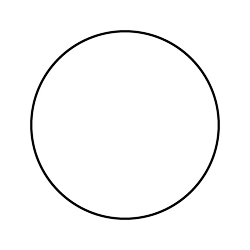
\includegraphics[width=\linewidth]{../data/virtual_0_1.png}
        \subcaption{$0_1$}
    \end{minipage}
    \begin{minipage}[b]{.14\linewidth}
        \centering
        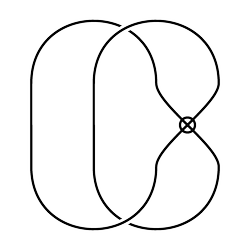
\includegraphics[width=\linewidth]{../data/virtual_2_1.png}
        \subcaption{$2_1$}
    \end{minipage}
    \begin{minipage}[b]{.14\linewidth}
        \centering
        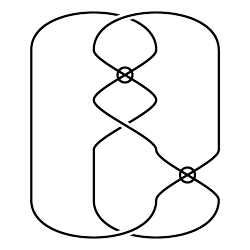
\includegraphics[width=\linewidth]{../data/virtual_3_1.png}
        \subcaption{$3_1$}
    \end{minipage}
    \begin{minipage}[b]{.14\linewidth}
        \centering
        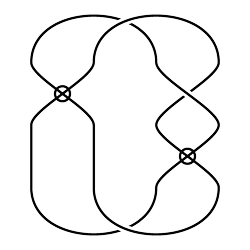
\includegraphics[width=\linewidth]{../data/virtual_3_7.png}
        \subcaption{$3_7$}
    \end{minipage}
    \begin{minipage}[b]{.14\linewidth}
        \centering
        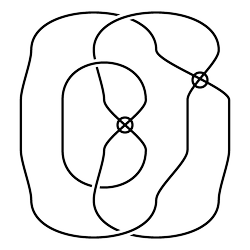
\includegraphics[width=\linewidth]{../data/virtual_4_1.png}
        \subcaption{$4_1$}
    \end{minipage}
    \begin{minipage}[b]{.14\linewidth}
        \centering
        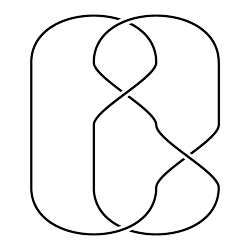
\includegraphics[width=\linewidth]{../data/virtual_4_108.png}
        \subcaption{$4_{108}$}
    \end{minipage}
\end{figure}
\end{comment}

Podamy teraz definicję równoważności dla węzłów singularnych, zupełnie analogicznie do definicji \ref{def:equivalent_knots_2} dla zwykłych węzłów.

\begin{definition}[płaski dysk]
    Niech $A$ będzie wierzchołkiem węzła singularnego $K$, $B_A$ jego małym domkniętym otoczeniem, zaś $P_A$ płaszczyzną, która zawiera $B_A \cap K$, mały fragment węzła wokół wierzchołka.
    Dysk $P_A \cap B_A$ nazywamy płaskim dyskiem wokół wierzchołka $A$.
\end{definition}

\begin{definition}
    Dwa singularne węzły $K, L$ są równoważne, co zapisujemy jako $K = L$, jeśli istnieje zachowujący orientację homeomorfizm $\varphi$ przestrzeni $\R^3$ w~siebie, który przenosi jeden węzeł na drugi: $\varphi(K) = L$ oraz indukuje bijekcję między rodzinami płaskich dysków $K$ i~$L$.
\end{definition}

Ten drugi warunek gwarantuje nam, że skrzyżowania wokół podwójnych punktów nie ulegną zniszczeniu.
Istnieje podobne kryterium dla diagramów, odpowiednik twierdzenia Reidemeistera.

\begin{proposition}
    Dwa singularne diagramy są równoważne dokładnie wtedy, kiedy można między nimi przejść przy użyciu ciągu izotopii otaczających, ruchów Reidemeistera oraz operacji $\Omega$:
\begin{comment}
    \[
    \begin{tikzpicture}[baseline=-0.65ex, scale=0.1]
    \begin{knot}[clip width=5, end tolerance=1pt, flip crossing/.list={1,2,3,4}]
        \strand[semithick] (-15, 5) [in=up,out=right] to (5, 0) [in=right,out=down] to (-15, -5);
        \strand[semithick] (-2, -2) to (-10, -10);
        \strand[semithick] (-2, 2) to (-10, 10);
        \strand[semithick] (2, -2) to (10, -10);
        \strand[semithick] (2, 2) to (10, 10);
        \draw[semithick] (2, 2) to (-2, -2);
        \draw[semithick] (2, -2) to (-2, 2);
        \draw[black,fill=black] (0,0) circle (.5);
    \end{knot}
    \end{tikzpicture}
    \quad\cong_\Omega\quad
    \begin{tikzpicture}[baseline=-0.65ex, scale=0.1]
    \begin{knot}[clip width=5, end tolerance=1pt, flip crossing/.list={1,2,3,4}]
        \strand[semithick] (-15, 5) [in=up,out=right] to (-5, 0) [in=right,out=down] to (-15, -5);
        \strand[semithick] (-2, -2) to (-10, -10);
        \strand[semithick] (-2, 2) to (-10, 10);
        \strand[semithick] (2, -2) to (10, -10);
        \strand[semithick] (2, 2) to (10, 10);
        \draw[semithick] (2, 2) to (-2, -2);
        \draw[semithick] (2, -2) to (-2, 2);
        \draw[black,fill=black] (0,0) circle (.5);
    \end{knot}
    \end{tikzpicture}
    \quad\cong_\Omega\quad
    \begin{tikzpicture}[baseline=-0.65ex, scale=0.1]
    \begin{knot}[clip width=5, end tolerance=1pt]
        \strand[semithick] (-15, 5) [in=up,out=right] to (5, 0) [in=right,out=down] to (-15, -5);
        \strand[semithick] (-2, -2) to (-10, -10);
        \strand[semithick] (-2, 2) to (-10, 10);
        \strand[semithick] (2, -2) to (10, -10);
        \strand[semithick] (2, 2) to (10, 10);
        \draw[semithick] (2, 2) to (-2, -2);
        \draw[semithick] (2, -2) to (-2, 2);
        \draw[black,fill=black] (0,0) circle (.5);
    \end{knot}
    \end{tikzpicture}
    \]
\end{comment}
\end{proposition}

Załóżmy teraz, że mamy jakiś niezmiennik węzłów $v$ o~wymiernych wartościach i~chcemy przedłużyć go do niezmiennika $\hat v$ węzłów singularnych.
Najprościej zrobić to rekurencyjnie.
Niech $\hat v$ będzie już określony dla węzłów singularnych o co najwyżej $n - 1$ wierzchołkach i~wybierzmy dowolny węzeł i diagram o~$n$ wierzchołkach.
Okazuje się, że jeżeli położymy
\begin{comment}
\begin{equation}
    \hat v\left(\SingularCrossing\right) = \hat v\left(\MediumSkeinPlus\right) - \hat v\left(\MediumSkeinMinus\right),
\end{equation}
\end{comment}
to dostaniemy dobrze określoną funkcję: jeżeli $L = K$ jest tym samym węzłem singularnym z~innym diagramem, to $\hat v(L) = \hat v(K)$.

Funkcję $\hat v$ nazywamy niezmiennikiem singularnym indukowanym przez niezmiennik węzłów $v_0$.

\begin{definition}[rząd niezmiennika]
\label{def:vassiliev_order}%
\index{rząd niezmiennika}%
    Niech $v$ będzie niezmiennikiem singularnym.
    Mówimy, że $v$ jest niezmiennikiem Wasiljewa rzędu co najwyżej $n$, jeśli dla dowolnego singularnego węzła $K$ o $n + 1$ wierzchołkach zachodzi $v(K) = 0$.
    Jeśli dodatkowo $v$ nie jest rzędu co najwyżej $n - 1$, to mówimy, że jest rzędu dokładnie $n$.
\end{definition}

Czas na garść przykładów.

\begin{example}
    Niech $K$ będzie węzłem, zaś $\conway_K(t) = \sum_k \conway_{2k} z^{2k}$ jego wielomianem Conwaya.
    Współczynnik $\conway_{2k}$ indukuje niezmiennik Wasiljewa rzędu dokładnie $2k$.
\end{example}

\begin{proof}
    Jak pokazuje Chmutow w \cite{chmutov12}, porównanie relacji kłębiastej dla wielomianu Conwaya z tą dla niezmienników Wasiljewa pokazuje, że wielomian Conwaya singularnego węzła o $m$ punktach podwójnych jest podzielny przez $z^m$, co pokazuje, że $c_{2k}$ jest niezmiennikiem rzędu co najwyżej $2k$.

    Bar-Natan w 1991 pokazał, że jest niezmiennikiem rzędu dokładnie $2k$.
\end{proof}

\index{hipoteza!Lin-Wanga}%
Lin oraz Wang \cite{wang96} w~1994 roku na podstawie niezmienników małych rzędów, to jest $v_2$ oraz $v_3$, wysunęli następującą hipotezę: istnieje uniwersalna stała $C$ taka, że
\begin{equation}
    |v_k(K)| \le C (\crossing K)^k.
\end{equation}

Hipotezę wkrótce udowodniono, najpierw dla węzłów (Bar-Natan, \cite{barnatan95}), nieco później także dla splotów (Stojmenow, \cite{stoimenow_01}).
Wartość stałej $C$ trudno obliczyć, dlatego Stojmenow zaproponował \cite[problem 1.17]{ohtsuki02} ograniczenie się do przypadku $v_k = \conway_k$.

\begin{conjecture}
    Niech $L$ będzie splotem.
    Wtedy
    \begin{equation}
        |\conway_k(L)| \le \frac{(\crossing L)^k}{2^kk!}.
    \end{equation}
\end{conjecture}

Nierówność jest nietrywialna tylko dla splotu $L$ z~$k+1, k-1, \ldots$ składowymi; trywialna dla $k = 0$, łatwa dla $k=1$ (wtedy $\conway_1$ jest indeksem zaczepienia splotów o~dwóch składowych) oraz udowodniona dla węzłów i~$k=2$ przez Polyaka, Viro w~2001 (\cite{polyak01}).

\begin{example}
    Niech $\jones_K(t)$ będzie wielomianem Jonesa węzła $K$.
    Dokonajmy podstawienia
    \begin{equation}
        t := e^x = 1 + x + \frac{x^2}{2} + \frac{x^3}{6} + \ldots,
    \end{equation}
    a~następnie rozwińmy wynik w~szereg Taylora:
    \begin{equation}
        \jones_K(e^x) = \sum_{k = 0}^\infty b_k x^k.
    \end{equation}
    Współczynnik $b_{k}$ indukuje niezmiennik Wasiljewa rzędu co najwyżej $k$.
\end{example}

Ten i podobne wyniki dla wielomianów HOMFLY, Kauffmana uzyskała Birman z~Linem w \cite{birman93}.
Praca ta znacznie uprościła oryginalne techniki Wasiljewa.
Patrz też \cite[s. 56]{chmutov12}.

\begin{example}[s. 311 w \cite{murasugi96}]
    Niech $K$ będzie węzłem, zaś $f(t)$ rozwinięciem Taylora wokół $t = 1$ dla wielomianu Jonesa:
    \begin{equation}
        f(t) = \sum_{k = 0}^\infty c_k (t-1)^k.
    \end{equation}
    Współczynnik $c_{k}$ indukuje niezmiennik Wasiljewa rzędu co najwyżej $k$.
\end{example}

Pójdźmy w ślad za Murasugim i zdefiniujmy nieskończoną rodzinę węzłów wirtualnych $K[p, q]$, gdzie $p$ jest liczbą wierzchołków, zaś $|q|$ liczbą klasycznych skrzyżowań.
Jeśli $q < 0$, wszystkie skrzyżowania odwracamy:
% \begin{comment}
\begin{figure}[H]
  \centering
  \[
\begin{tikzpicture}[baseline=-0.65ex, scale=0.1]
\begin{knot}[clip width=5, end tolerance=1pt, flip crossing/.list={2}]
    % left part
    \draw[thick] (5, 0) [in=-60, out=-120] to (-5, 0) [in=60, out=120] to (-15, 0) [in=-60, out=-120] to (-25, 0) [in=60, out=120] to (-35, 0) [in=180, out=-120] to (-35, -10);
    \draw[thick] (5, 0) [in=60, out=120] to (-5, 0) [in=-60, out=-120] to (-15, 0) [in=60, out=120] to (-25, 0) [in=-60, out=-120] to (-35, 0) [in=-180, out=120] to (-35, 10);
    % right part
    \strand[thick] (5, 0) [in=120, out=60] to (15, 0) [in=-120, out=-60] to (25, 0) [in=120, out=60] to (35, 0) [in=0, out=-60] to (35, -10);
    \strand[thick] (5, 0) [in=-120, out=-60] to (15, 0) [in=120, out=60] to (25, 0) [in=-120, out=-60] to (35, 0) [in=0, out=60] to (35, 10);
    % external lines
    \draw[thick,Latex-] (-35, 10) to (35, 10);
    \draw[thick,Latex-] (-35, -10) to (35, -10);
    \draw[black,fill=black] (5,0) circle (1);
    \draw[black,fill=black] (-5,0) circle (1);
    \draw[black,fill=black] (-15,0) circle (1);
    \draw[black,fill=black] (-25,0) circle (1);
    \draw[black,fill=black] (-35,0) circle (1);
\end{knot}
\end{tikzpicture}\]
  \caption{Węzeł singularny $K[p, q]$ dla $p = 2, q = 10$.}
\end{figure}
% \end{comment}

\begin{proposition}
    Następujące funkcje nie są niezmiennikami Wasiljewa: indeks skrzyżowaniowy $\operatorname{cr}$, liczba gordyjska $\operatorname{u}$, indeks mostowy $\operatorname{br}$, indeks warkoczowy $\operatorname{b}$, genus $g$, sygnatura $\sigma$.
\end{proposition}

Wynik był znany już w latach 90., na przykład Birman w \cite{birman93} pokazała, że liczba gordyjska nie jest niezmiennikiem Wasiljewa.

\begin{proof}
    Żaden z tych niezmienników nie znika na singularnym węźle $K[n+1, n]$.
\end{proof}

Udowodnimy kilka najprostszych własności niezmienników Wasiljewa.

% Niezmiennik Wasiljewa węzła z~pętelką to zero.

\begin{proposition}
    Każdy niezmiennik Wasiljewa rzędu zero jest funkcją stałą.
\end{proposition}

\begin{proof}
    Niech $v$ będzie niezmiennikiem rzędu zero i~znika na każdym singularnym węźle o~jednym wierzchołku.
    Relacja kłębiasta mówi, że $v(\LittleLeftCrossing) = v(\LittleRightCrossing)$, to znaczy odwrócenie dowolnego skrzyżowania nie zmienia wartości niezmiennika.

    Z lematu \ref{lem:unknotting_well_defined} wiemy jednak, że każdy węzeł można zmienić w niewęzeł odwracając niektóre skrzyżowania.
    Wynika stąd, że $v(K) = v(\LittleUnknot)$ dla każdego singularnego węzła $K$, co należało udowodnić 
\end{proof}

\begin{proposition}
    Nie istnieje niezmiennik Wasiljewa rzędu jeden.
\end{proposition}

% The Casson knot invariant (to be distinguished from the better-known Casson invariant) is defined to be the Vassiliev knot invariant v_2, which turns out to be \alexander_k''(1) / 2 , where \alexander_k is the Alexander polynomial of k.
% \index{niezmiennik!Cassona}
% It can be characterized as the unique Vassiliev invariant of degree 2 that takes value 0 on the trivial knot and value 1 on the trefoil knot.

(Na podstawie pierwszych stron \cite{chmutov12}).
Oznaczmy przez $\mathcal V_n$ zbiór niezmienników Wasiljewa rzędu co najwyżej $n$, o~wartościach w zbiorze liczb zespolonych $\C$.
Z definicji \ref{def:vassiliev_order} wynika, że $\mathcal V_n$ jest przestrzenią wektorową nad ciałem $\C$ oraz $\mathcal V_n \subseteq \mathcal V_{n+1}$ i mamy rosnącą filtrację
\begin{equation}
    \mathcal V_0 \subseteq \mathcal V_1 \subseteq \mathcal V_2 \subseteq \ldots \subseteq \mathcal V := \bigcup_{n=0}^\infty \mathcal V_n.
\end{equation}

Oznaczmy wymiar przestrzeni $\mathcal V_n / \mathcal V_{n-1}$ przez $d_n$.
Dla wyższych rzędów nie dość, że nie znamy dokładnych wartości ciągu $d_n$, to dolne i górne ograniczenia asymptotyczne są od siebie bardzo różne: górne jest niemalże silnią, dolne natomiast jest podwykładnicze.

\begin{proposition}
    $d_n < (2n-1)!!$.
\end{proposition}

\begin{proposition}[Chmutov i Duzhin, 1993]
    $d_n < (n-1)!$.
\end{proposition}

\begin{proposition}[Ng, 1995]
    $d_n < \frac 12 (n-2)!$.
\end{proposition}

\begin{proposition}[Stojmenow, 1996]
    Ciąg $d_n$ rośnie wolniej niż $n! \cdot (11/10)^n$.
\end{proposition}

\begin{proposition}[Bollobas i  Riordan, 2000]
    $d_n \lesssim n! / (2 \log 2 + O(1))^n$.
\end{proposition}

\begin{proposition}[Zagier, 2001]
    Niech $a < \frac 1 6 \pi^2$ będzie stałą.
    Wtedy
    \begin{equation}
        \dim \mathcal V_n / \mathcal V_{n-1} \lesssim \frac{n!}{a^n}.
    \end{equation}
\end{proposition}

\begin{proof}
    Zagier znalazł to ograniczenie przy użyciu szeregów Dirichleta w \cite{zagier01}.
\end{proof}

Zanim przejdziemy do ograniczeń z dołu, zdefinujmy jeszcze jedną przestrzeń, $\mathcal P_n \subseteq \mathcal V_n$.
Składa się z~tych niezmienników Wasiljewa, które są jednocześnie morfizmami, to znaczy spełniają równość $v(K_1 \shrap K_2) = v(K_1) + v(K_2)$.
Każdy niezmiennik jest wielomianową kombinacją niezmienników pierwotnych.

\begin{proposition}[Chmutov, Duzhin i Lando, 1994]
    $\dim \mathcal P_n \ge 1$.
\end{proposition}

\begin{proposition}[Melvin i Morton, Chmutov i Varchenko, 1995]
    $\dim \mathcal P_n \ge [n/2]$.
\end{proposition}

\begin{proposition}[Duzhin, 1996]
    $\dim \mathcal P_n \gtrsim \frac{1}{96} n^2$.
\end{proposition}

\begin{proposition}[Chmutov i Duzhin, 1997]
    $\dim \mathcal P_n \gtrsim n^{\log_b n}$ dla $b > 4$.
\end{proposition}

\begin{proposition}[Koncewicz, 1997]
    $\dim \mathcal P_n \gtrsim \exp (\pi \sqrt{n/3})$.
\end{proposition}

\begin{proposition}[Dasbach, 2000]
    $\dim \mathcal P_n \gtrsim \exp (c \sqrt{n})$ dla każdej stałej $c < \pi \sqrt{2/3}$.
\end{proposition}

Ograniczenie Dasbacha pozostaje najlepsze (stan na 2011 rok).

\begin{corollary}
    Niech $a < \frac 1 6 \pi^2$ będzie stałą.
    Wtedy
    \begin{equation}
        \exp \left(\frac {n}{\log_a n} \right) \lesssim \dim \mathcal V_n / \mathcal V_{n-1}.
    \end{equation}
\end{corollary}

\begin{proof}
    Dasbach w \cite{dasbach00}.
\end{proof}

Dokładny wymiar przestrzeni $\mathcal V_n$ jest znany tylko dla $n \le 12$.
Poniższa tabela ma dość ciekawą historię.
Wasiljew znalazł ręcznie wartości w kolumnach dla $n \le 4$ w 1990 roku.
Potem Bar-Natan napisał komputerowy program rozwiazujący pewne równania liniowe i~znalazł tak wymiary przestrzeni $\mathcal V_n$ dla $n \le 9$, miało to miejsce w roku 1993.
Wreszcie Kneissler cztery lata później znalazł dolne oraz górne ograniczenia: dolne oparte o znaczone powierzchnie, górne pochodzące od algebry Vogela (\cite{kneissler97}).
\index{algebra!Vogela}
\index{powierzchnia!znaczona}
% DICTIONARY;marked surface;powierzchnia znaczona
Dla $n \le 12$ ograniczenia te pokrywają się!

\renewcommand*{\arraystretch}{1.4}
\footnotesize
\begin{longtable}{lcccccccccccccc}
\hline
    $n$ & $0$ & $1$ & $2$ & $3$ & $4$ & $5$ & $6$ & $7$ & $8$ & $9$ & $10$ & $11$ & $12$ \\ \hline \endhead
    $\dim \mathcal V_n$ & $1$ & $1$ & $2$ & $3$ & $6$ & $10$ & $19$ & $33$ & $60$ & $104$ & $184$ & $316$ & $548$ \\
    $\dim \mathcal V_n / \mathcal V_{n-1}$ & $1$ & $0$ & $1$ & $1$ & $3$ & $4$ & $9$ & $14$ & $27$ & $44$ & $80$ & $132$ & $232$ \\
    \hline
\end{longtable}
\normalsize

% kneissler97 podaje inny ciąg: 0, 1, 1, 2, 3, 5, 8, 12, 18, 27, 39, 55... (rk Pm), nasz nazywając (rk Am / rk Arm)
% Am: Z<circle diagrams of degree m> / Z<STU relations>
% Arm: Am / Z<FI relations>
% Pm: podmoduł Am generowany przez spójne diagramy

Okazuje się, że wartość niezmiennika Wasiljewa $v$ nie zależy wprost od tego, jak zaplątany jest węzeł singularny $K$, ale od tego, jak ułożone są wierzchołki wzdłuż węzła. Standardową metodą kodowania tej informacji jest diagram cięciw.

\begin{definition}[diagram cięciw]
% DICTIONARY;diagram, chord;diagram, cięciw
\index{diagram cięciw}%
    Zorientowany okrąg razem z~$2n$ punktami leżącymi na nim (oraz~połączonymi w pary) z~dokładnością do zachowujących orientację homeomorfizmów nazywamy diagramem cięciw rzędu $n$, albo stopnia $n$.
\end{definition}

\begin{figure}[H]
    \centering
    \begin{minipage}[b]{.18\linewidth}
        \centering
        $\begin{tikzpicture}[baseline=-0.65ex,scale=0.15]
            \useasboundingbox (-7, -5) rectangle (7, 5);
            \draw[thick] (-0, 0) circle (5);
            \draw[thick, brown] (0:5) to (180:5);
            \draw[thick, brown] (60:5) [in=-60,out=-120] to (120:5);
            \draw[thick, brown] (-60:5) [in=60,out=120] to (-120:5);
        \end{tikzpicture}$
        \subcaption{}
    \end{minipage}
    \begin{minipage}[b]{.18\linewidth}
        \centering
        $\begin{tikzpicture}[baseline=-0.65ex,scale=0.15]
            \useasboundingbox (-7, -5) rectangle (7, 5);
            \draw[thick] (-0, 0) circle (5);
            \draw[thick, brown] (0:5) [in=-120, out=180] to (60:5);
            \draw[thick, brown] (120:5) [in=0, out=-60] to (180:5);
            \draw[thick, brown] (240:5) [in=120, out=60] to (300:5);
        \end{tikzpicture}$
        \subcaption{}
    \end{minipage}
    \begin{minipage}[b]{.18\linewidth}
        \centering
        $\begin{tikzpicture}[baseline=-0.65ex,scale=0.15]
            \useasboundingbox (-7, -5) rectangle (7, 5);
            \draw[thick] (-0, 0) circle (5);
            \draw[thick, brown] (0:5) [out=180, in=-60] to (120:5);
            \draw[thick, brown] (60:5) [in=0,out=-120] to (180:5);
            \draw[thick, brown] (240:5) [in=120, out=60] to (300:5);
        \end{tikzpicture}$
        \subcaption{}
    \end{minipage}
    \begin{minipage}[b]{.18\linewidth}
        \centering
        $\begin{tikzpicture}[baseline=-0.65ex,scale=0.15]
            \useasboundingbox (-7, -5) rectangle (7, 5);
            \draw[thick] (-0, 0) circle (5);
            \draw[thick, brown] (0:5) to (180:5);
            \draw[thick, brown] (60:5) [in=120,out=-120] to (300:5);
            \draw[thick, brown] (120:5) [in=60, out=-60] to (240:5);
        \end{tikzpicture}$
        \subcaption{}
    \end{minipage}
    \begin{minipage}[b]{.18\linewidth}
        \centering
        $\begin{tikzpicture}[baseline=-0.65ex,scale=0.15]
            \useasboundingbox (-7, -5) rectangle (7, 5);
            \draw[thick] (-0, 0) circle (5);
            \draw[thick, brown] (0:5) to (180:5);
            \draw[thick, brown] (60:5) to (240:5);
            \draw[thick, brown] (120:5) to (300:5);
        \end{tikzpicture}$
        \subcaption{}
    \end{minipage}
    \caption{Wszystkie pięć diagramów cięcin stopnia 3}
\end{figure}

\begin{proposition}
    Niech $K_1, K_2$ będą dwoma singularnymi węzłami o~tym samym diagramie cięciw, zaś $v$~niezmiennikiem Wasiljewa.
    Wtedy $v(K_1) = v(K_2)$.
\end{proposition}

\begin{proof}
    Umieśćmy węzły singularne $K_1, K_2$ w przestrzeni tak, by ich wierzchołki oraz obie gałęzie wychodzące z wierzchołków leżały tak samo. Wtedy można tak zdeformować łuki $K_1$ tak, by jedynymi osobliwościami, jakie się pojawią lub znikną, były podwójne punkty.
    Teraz kłębiasta Wasiljewa mówi, że wartość $v$ nie zmienia się podczas tego procesu, zatem $v(K_1) = v(K_2)$, co należało okazać.
    % chmutov12
    % TODO: (\cite{duzhin12}, prop. 3.4.2)
\end{proof}

\begin{definition}[symbol niezmiennika]
    Niech $v$ będzie niezmiennikiem Wasiljewa.
    Obcięcie $v$ do zbioru węzłów singularnych o~dokładnie $n$ wierzchołkach traktowane jako funkcja ze zbioru diagramów cięcin nazywamy symbolem tego niezmiennika.
\end{definition}

Jeśli $v_1, v_2$ są niezmiennikami Wasiljewa rzędu co najwyżej $n$ o~tych samych symbolach, to ich różnica jest niezmiennikiem rzędu co najwyżej $n - 1$.
Oznacza to, że przestrzeń $\mathcal V_n/\mathcal V_{n-1}$ pokrywa się z przestrzenią wszystkich symboli niezmienników Wasiljewa rzędu co najwyżej $n$.
Zbiór diagramów cięcin rzędu $n$ jest skończony, więc przestrzeń funkcji na tym zbiorze też jest skończona, a zatem przestrzenie $\mathcal V_n$ są skończonego wymiaru.

Symbol nie jest byle jaką funkcją, spełnia dwie relacje:

\begin{figure}[H]
$$
\begin{tikzpicture}[baseline=-0.65ex,scale=0.15]
    \useasboundingbox (-7, -5) rectangle (7, 5);
    \draw[densely dotted] (-0, 0) circle (5);
    \draw[thick, brown] (20*17:5) [out=180+17*20, in=down] to (0:2) [in=180+1*20, out=up] to (20*1:5);
    \draw[thick] (20*16:5) arc (20*16:20*20:5);
\end{tikzpicture}
\mapsto 0
$$
\caption{Relacja ,,one-term'' (1T albo FI?)}
\end{figure}
oraz
\begin{figure}[H]
$$
\begin{tikzpicture}[baseline=-0.65ex,scale=0.15]
    \useasboundingbox (-7, -5) rectangle (7, 5);
    \draw[densely dotted] (-0, 0) circle (5);
    \draw[thick, brown] (20*1:5) [in=180+13*20, out=180+1*20] to (20*13:5);
    \draw[thick, brown] (20*6:5) [in=180+12*20, out=180+6*20] to (20*12:5);
    \draw[thick] (20*5 :5) arc (20*5 :20*8 :5);
    \draw[thick] (20*11:5) arc (20*11:20*14:5);
    \draw[thick] (20*17:5) arc (20*17:20*20:5);
\end{tikzpicture}
-
\begin{tikzpicture}[baseline=-0.65ex,scale=0.15]
    \useasboundingbox (-7, -5) rectangle (7, 5);
    \draw[densely dotted] (-0, 0) circle (5);
    \draw[thick, brown] (20*0:5) [in=180+12*20, out=180+0*20] to (20*12:5);
    \draw[thick, brown] (20*7:5) [in=180+13*20, out=180+7*20] to (20*13:5);
    \draw[thick] (20*5 :5) arc (20*5 :20*8 :5);
    \draw[thick] (20*11:5) arc (20*11:20*14:5);
    \draw[thick] (20*17:5) arc (20*17:20*20:5);
\end{tikzpicture}
+
\begin{tikzpicture}[baseline=-0.65ex,scale=0.15]
    \useasboundingbox (-7, -5) rectangle (7, 5);
    \draw[densely dotted] (-0, 0) circle (5);
    \draw[thick, brown] (20*0:5) [in=180+6*20, out=180+0*20] to (20*6:5);
    \draw[thick, brown] (20*1:5) [in=180+13*20, out=180+1*20] to (20*13:5);
    \draw[thick] (20*5 :5) arc (20*5 :20*8 :5);
    \draw[thick] (20*11:5) arc (20*11:20*14:5);
    \draw[thick] (20*17:5) arc (20*17:20*20:5);
\end{tikzpicture}
-
\begin{tikzpicture}[baseline=-0.65ex,scale=0.15]
    \useasboundingbox (-7, -5) rectangle (7, 5);
    \draw[densely dotted] (-0, 0) circle (5);
    \draw[thick, brown] (20*0:5) [in=180+12*20, out=180+0*20] to (20*12:5);
    \draw[thick, brown] (20*1:5) [in=180+7*20, out=180+1*20] to (20*7:5);
    \draw[thick] (20*5 :5) arc (20*5 :20*8 :5);
    \draw[thick] (20*11:5) arc (20*11:20*14:5);
    \draw[thick] (20*17:5) arc (20*17:20*20:5);
\end{tikzpicture}
\mapsto 0.
$$
\caption{Relacja ,,four-term'' (4T)}
\end{figure}

Diagramy mogą mieć więcej cięciw z końcami tam, gdzie linia jest kropkowana, natomiast wszystkie końce cięciw na czarnych, pogrubionych łukach zostały zaznaczone explicite.

Zastosowaliśmy tutaj mały skrót dla oszczędności miejsca: oczywiście nie umiemy jeszcze odejmować od siebie diagramów, dlatego powyższe relacje należy rozumieć tak, że na każdym diagramie liczymy symbol niezmiennika i porównujemy tak otrzymane liczby zespolone.

\begin{definition}[układ ciężarów]
    Funkcję określoną na zbiorze diagramów $n$ cięciw, która spełnia relacje 1T oraz 4T, nazywamy układem ciężarów.
% DICTIONARY;weight system;układ ciężarów
\end{definition}

Okazuje się, że wszystkie zależności, jakie występują między niezmiennikami Wasiljewa, są konsekwencjami relacji 1T oraz 4T.
Mówi o~tym głębokie twierdzenie Koncewicza:

\begin{proposition}
    Każdy układ ciężarów jest symbolem pewnego niezmiennika Wasiljewa. % rzędu co najwyżej $n$ - nie mieści się, przenosi samo $n$ do nowej linii.
\end{proposition}

\begin{proof}
    Koncewicz w \cite{kontsevich93}. % chmutow12/chmutov11 theorem 3.4
\end{proof}

\begin{definition}[chiński znak]
    Spójny graf złożony z pojedynczego zorientowanego okręgu oraz pewnej liczby niezorientowanych, kreskowanych linii, które mogą się spotykać w~jednym z dwóch typów wierzchołków:
    \begin{itemize}
        \item wewnętrznych wierzchołkach, gdzie spotykają się trzy kreskowane linie -- te są zorientowane (zgodnie lub przeciwnie do ruchu wskazówek zegara)
        \item zewnętrznych wierzchołkach, gdzie kreskowane linie kończą się na okręgu.
    \end{itemize}
\end{definition}

Diagramy cięciw modulo relacja 4T jest tym samym, co algebra chińskich znaków modulo relacja STU.
W~tej drugiej spełnione są jeszcze relacje AS oraz IHX, nie mam siły tego rysować, ale wszystko można znaleźć w pracy Bar-Natana \cite{barnatan_95}.

\begin{tobedone}
    % DICTIONARY;actuality table;tablica rzeczywistości
    \index{tablica rzeczywistości?}
    Actuality tables.
\end{tobedone}

Stojmenow w \cite{stoimenow_01} pokazał, że niezmienniki Wasiljewa każdego rzędu można wyznaczyć w~skończonym czasie.
Dokładniej:

\begin{proposition}
    Każdy niezmiennik Wasiljewa rzędu co najwyżej $k$ jest jednoznacznie określony przez swoje wartości na alternujących węzłach o co najwyżej $2k^2 + k$ skrzyżowaniach.
\end{proposition}

% kneissler97: Corollary 2.5: up to degree twelce can't distinguish knots from their inverses.

Niezmienniki Wasiljewa nie są zupełne.
Ohyama dla każdego węzła $K$ i~liczby naturalnej $n$ wskazał jawnie nieskończoną rodzinę złożonych węzłów, których niezmienniki rzędu co najwyżej $n$ nie odróżniają od $K$ (\cite{ohyama95}).
Stanford rozszerzył ten wynik: w~\cite{stanford96} udowodnił, że dla każdego splotu $L$ istnieje nieskończona rodzina pierwszych, nierozszczepialnych, alternujących splotów nieodróżnialnych takimi niezmiennikami.

Z drugiej strony, Chmutow i inni piszą w \cite{duzhin12}, że sześć niezmienników rzędu co najwyżej 4 wystarcza do odróżnienia dowolnych dwóch węzłów pierwszych do 8 skrzyżowań.

W 1993 roku Maxim Koncewicz pokazał, że dla każdego węzła można policzyć pewną całkę (teraz nazywaną całką Koncewicza), która jest uniwersalnym niezmiennikiem Wasiljewa.
\index{całka Koncewicza}
Oznacza to, że z jej wartości można odtworzyć wszystkie inne niezmienniki skończonego typu.
Bar-Natan w 1995 roku znalazł wartość tej całki dla niewęzła:
\begin{equation}
    I (\LittleUnknot) = \exp \left(\sum_{n=0}^\infty b_{2n} w_{2n}\right),
\end{equation}
gdzie $b_{2n}$ to zmodyfikowane liczby Bernoulliego o funkcji tworzącej
\begin{equation}
    \sum_{n=0}^\infty b_{2n} x^{2n} = \frac 12 \log \frac {e^{x/2} - e^{-x/2}}{x/2},
\end{equation}
zaś $w_{2n}$ to ,,koła'': diagramy okręgu z doczepionymi $2n$ promieniami.
Liniową kombinację należy rozumieć jako element algebry chińskich znaków, opisanej w następnej wersji tej książki.
\index{algebra!chińskich znaków}
Następnie Marché w~2003 roku znalazł wartości całki dla węzłów torusowych (\cite{marche04}).
Wygląda na to, że nikt nie odważył się dokonać tego dla innych węzłów (stan na 2019).

\begin{conjecture}
    \label{con:vassilliev}
    Uniwersalny niezmiennik Wasiljewa jest zupełny.
\end{conjecture}

Całka Koncewicza jest mocniejsza od każdego wielomianowego niezmiennika, jaki dotąd poznaliśmy, wliczając w to wielomiany Alexandera, Jonesa, HOMFLY oraz Kauffmana.
Wynika stąd, że stanowić będzie dużo trudniejszy problem niż dowód hipotezy \ref{con:jones} mówiącej, że wielomian Jonesa wykrywa niewęzły.

% DICTIONARY;link, string;splot, sznurkowy
Chmutov, Duzhin wspominają w bardzo czytelnie napisanym artykule \cite{chmutov05}, że hipoteza \ref{con:vassilliev} jest prawdziwa dla splotów sznurkowych i warkoczy, jak dowiedziono w \cite{kohno87}, \cite{barnatandror95}.

\index{niezmiennik!Wasiljewa|(}

% koniec sekcji niezmienniki Wasiljewa


\chapter{Topologia algebraiczna}
W tym rozdziale poznamy niezmienniki wywodzące się z~topologii algebraicznej przy użyciu maszynerii topologii algebraicznej, na tyle, na ile to możliwe.
Zaczniemy od grupy splotu (czyli grupy jego dopełnienia), potem poznamy jej prezentację Wirtingera i~jeszcze raz spotkamy pochodną Foxa.
Następnie odkryjemy powierzchnie Seiferta, jeszcze jedno ,,źródło'' genusu, wyznacznika, sygnatury, niezmiennika Arfa czy przede wszystkim wielomianu Alexandera.
Na koniec powiemy krótko, czym są homologie, w szczególności homologie Chowanowa.

% koniec wstępu do rozdziału 4

\section{Grupa węzła}
Ponieważ dopełnienie dowolnego węzła, zarówno w przestrzeni $\R^3$ jak i $S^3$, jest łukowo spójne, jego grupa podstawowa nie zależy od wyboru punktu bazowego.
Dzięki temu poniższa definicja ma sens:

\begin{definition}[grupa węzła]
\index{grupa!węzła}%
    Niech $K$ będzie węzłem.	
    Grupę podstawową jego dopełnienia,
    \begin{equation}
    	\pi(L) := \pi_1 \left(\R^3 \setminus L\right),
    \end{equation}
    nazywamy grupą węzła i oznaczamy $\pi(K)$.
\end{definition}

Nie należy (i dosyć trudno jest) mylić grupy węzła z grupą kolorującą (patrz definicja \ref{def:colouring_group}).
Jak wkrótce się przekonamy, ta pierwsza jest zawsze nieskończona i poza grupą niewęzła, nieprzemienna.
Natomiast grupa kolorująca jest skończona dla splotów o~niezerowym wyznaczniku i zawsze przemienna.

Podamy najpierw kilka przykładów węzłów oraz ich grup.

\begin{example}
    Grupa niewęzła: $\Z$.
\end{example}

Z twierdzenia o pętli, czyli uogólnienia lematu Dehna wynika, że niewęzeł jest jedynym węzłem, którego grupą podstawową jest $\Z$.
% TODO: https://math.stackexchange.com/questions/3468034/knot-group-is-mathbbz-iff-k-is-the-unknot

\begin{example}
\label{exm:trefoil_group}%
    Grupa trójlistnika: $\langle x, y \mid x^2 = y^3\rangle$.
\end{example}

\begin{proof}
    Wynika to z (prezentacji Wirtingera i) równości
    % https://en.wikipedia.org/wiki/Tietze_transformations
    \begin{align}
        \pi_1(S^3 \setminus 3_1) & = \langle x, y, z \mid xz = yx, zy = xz, yx = zy \rangle \\
                                 & = \langle x, y \mid xyx = yxy \rangle \\
                                 & = \langle x, y, a, b \mid xyx = yxy, a = yx, b = xyx \rangle \\
                                 & = \langle x, a, b \mid xa = a^2x^{-1}, b = xa \rangle \\
                                 & = \langle a, b \mid b = a^2(ba^{-1})^{-1} \rangle \\
                                 & = \langle a, b \mid a^3 = b^2 \rangle,
    \end{align}
    prawdziwych na mocy transformacji Tietzego.
\end{proof}

Trójlistnik jest węzłem $(3, 2)$-torusowym, więc powyższy przykład stanowi szczególny przypadek grupy węzła torusowego.
Jej wyznaczenie to popularne ćwiczenie w~podręcznikach topologii algebraicznej:

\begin{example}
    Grupa węzła $(p,q)$-torusowego: $\langle x, y \mid x^p = y^q \rangle$.
\end{example}

\begin{proof}
    Wniosek z twierdzenia Seiferta-van Kampena, patrz \cite[s. 77]{kawauchi96} albo \cite[s. 47]{hatcher02}.
\end{proof}

\begin{example}
    Grupa ósemki: $\langle x, y \mid yxy^{{-1}}xy=xyx^{{-1}}yx \rangle$.
\end{example}

\begin{proposition}
    \label{prop:knot_group_invariant}
    Jeżeli węzły $L_1, L_2$ są równoważne, to grupy $\pi(L_1), \pi(L_2)$ są izomorficzne.
    Innymi słowy, grupa jest niezmiennikiem węzłów.
\end{proposition}

\begin{proof}
    Gdy dwa węzły są równoważne, istnieje izotopijny z~identycznością homeomorfizm $\R^3 \to \R^3$, który posyła pierwszy węzeł na drugi.
    Obcięty do dopełnień węzłów indukuje izomorfizm grup podstawowych.
\end{proof}

Na przykładzie grupy $\langle x,y,z \mid xyx=yxy,xzx=zxz\rangle$, która odpowiada zarówno sumie prostej różno-, jak i~jednoskrętnych trójlistników, widać że implikacja odwrotna nie zachodzi: mają one różne sygnatury (patrz uwaga za wnioskiem \ref{cor:acheiral_signature}).
Prawdziwe jest nawet ogólniejsze stwierdzenie:

\begin{proposition}
    Niech $K_1, K_2$ będą zorientowanymi węzłami.
    Wtedy węzłom $K_1 \shrap K_2$, $K_1 \shrap mr K_2$ odpowiadają izomorficzne grupy.
\end{proposition}

\begin{proof}
    Wniosek z twierdzeń o podgrupie południkowo-równoleżnikowej \cite[s. 75]{kawauchi96}.
\end{proof}

Twierdzenie odwrotne do faktu \ref{prop:knot_group_invariant} jest prawdziwe w klasie węzłów pierwszych:

\begin{proposition}
    Niech $K_1, K_2$ będą węzłami pierwszymi.
    Jeżeli ich grupy są izomorficzne, to same węzły są równoważne.
\end{proposition}

,,\emph{The group of a prime knot does not, however, necessarily determine the topological type of the exterior. Dehn hips on certain “essential” solid tori in the exteriors of torus knots and of cable knots produce Haken manifolds that are homotopically equivalent but not homeomorphic to the original exteriors and that, in fact, cannot be imbedded in $S^3$}'' (Whitten, \cite{whitten87}).
\index{rozmaitość!Hakena}%

\begin{proof}
\index[persons]{Gordon, Cameron}%
\index[persons]{Luecke, John}%
\index[persons]{Whitten, Wilbur}%
    % to jest kopia \cite[s. 76]{kawauchi96}
    Whitten pokazał w \cite{whitten87}, że węzły o~izomorficznych grupach mają homeomorficzne dopełnienia.
    Wkrótce po tym Gordon, Luecke udowodnili w~\cite{gordon89}, że nietrywialna chirurgia Dehna na nietrywialnym węźle nigdy nie daje sfery $S^3$, a~stąd wynika, że każdy homeomorfizm dopełnień węzłów można przedłużyć do homeomorfizmu $S^3$ w~siebie posyłającego jeden węzeł na drugi jako zbiory.
\index{chirurgia Dehna}%
\end{proof}

Waldhausen \cite{waldhausen68} pokazał dla pewnej dużej klasy 3-rozmaitości, że są scharakteryzowane topologicznie przez ich grupy podstawowe.
\index[persons]{Waldhausen, Friedhelm}%
Potem odkryto, że:

\begin{proposition}
    Grupa węzła wyznacza wartość jego genusu.
\end{proposition}
\begin{proof}[Niedowód]
    Jest to wniosek 3 z~pracy \cite{feustel78} Feustela.
\end{proof}
\begin{proposition}
    Grupa węzła złożonego wyznacza wartość jego liczby mostowej.
\end{proposition}
\begin{proof}[Niedowód]
    Jest to wniosek 3 z~pracy \cite{feustel78} Feustela.
\end{proof}

Wreszcie Thurston \cite{thurston82} jako efekt uboczny uzyskał kolejny wynik o grupie: hiperboliczne rozmaitości o skończonej objętości (domknięte rozmaitości lub takie, których brzeg jest zbudowany z torusów) są wyznaczone przez ich grupę podstawową.
\index[persons]{Thurston, William}%

\subsection{Grupa splotu}

Kawauchi \cite[s. 73]{kawauchi96} definiuje grupę splotu jako grupę podstawową jego dopełnienia.
Dla Milnora \cite{milnor54} grupą splotu był pewien iloraz\footnote{%
Niech $L$ będzie splotem w otwartej 3-rozmaitości $M$, $\pi(L)$ grupą podstawową dopełnienia $L$, zaś $L^i$ splotem powstałym przez usunięcie $i$-tego ogniwa.
Niech $A_i(L)$ oznacza jądro naturalnej inkluzji $\pi(L) \to \pi(L^i)$, zaś $[A_i]$ komutanta.
Wtedy $E(L) := [A_1][A_2] \cdots [A_n]$ jest podgrupą normalną $\pi(L)$.
Milnor nazywa iloraz $\pi(L) / E(L)$ grupą splotu.%
} tamtej grupy, dlatego należy zachować ostrożność i~sprawdzić, która konwencja obowiązuje.
% TODO: John Milnor (1954). Link groups. Ann. of Math. (2), 59, 177–195. https://mathscinet.ams.org/mathscinet/relay-station?mr=71020
My będziemy mieć do czynienia jedynie z~grupą podstawową dopełnienia.

\begin{example}
    Grupa splotu Hopfa: $\Z \oplus \Z$.
\end{example}

Kawauchi wspomina, że istnieją sploty, których grupa splotu nie odróżnia, podaje w~formie ćwiczenia \cite[s. 73]{kawauchi96}, że grupa sumy niespójnej splotów $L_1, L_2$ to $\pi(L_1) * \pi(L_2)$ i~przytacza twierdzenie:

\begin{proposition}
    Niech $L \subseteq S^3$ będzie splotem.
    Następujące warunki są równoważne:
    \begin{enumerate}
        \item splot $L$ nie jest rozszczepialny,
\index{splot!rozszczepialny}%
        \item splot $L$ jest niewęzłem lub jego dopełnienie jest rozmaitością Hakena o~nieściśliwym brzegu,
\index{rozmaitość!Hakena}%
        \item grupa podstawowa splotu $L$ jest nierozkładalna względem produktu wolnego.
    \end{enumerate}
\end{proposition}

\begin{proof}
    Z twierdzenia o pętli (niech $M$ będzie spójną 3-rozmaitością o niepustym brzegu, zaś $F$ powierzchnią na $\partial M$; jeżeli homomorfizm $\pi_1(F) \to \pi_1(M)$ indukowany przez inkluzję nie jest różnowartościowy, to istnieje dysk ściskający dla $F$ w $M$) i sferze (niech $M$ będzie spójną zorientowaną 3-rozmaitością, jeżeli $\pi_2(M)$ jest nietrywialna, to istnieje sfera właściwa w $M$) wynika, że $1 \implies 2$.
    Implikacja $2 \implies 3$ jest wnioskiem z hipotezy Knesera (niech $M$ będzie zwartą, spójną 3-rozmaitością, której brzeg jest pusty lub złożony z nieściśliwych powierzchni; jeśli $\pi_1(M) \cong G_1 * G_2$, to istnieje rozkład $M$ na sumę $M_1 \shrap M_2$ taką, że $\pi_1(M_i) \cong G_i$), zaś wynikanie $3 \implies 1$ jest oczywiste.
    To kończy dowód.
\end{proof}

\begin{corollary}
    Niech $L \subseteq S^3$ będzie splotem.
    Następujące warunki są równoważne:
    \begin{enumerate}
        \item grupa podstawowa splotu $L$ jest wolna, rangi $n$,
        \item splot $L$ jest trywialny, złożony z $n$ ogniw.
    \end{enumerate}
\end{corollary}

\begin{proposition}
    Niech $L \subseteq S^3$ będzie splotem.
    Następujące warunki są równoważne:
    \begin{enumerate}
        \item splot $L$ jest prosty i niepierścieniowaty\footnote{simple, anannular},
        \item grupa $\pi(L)$ jest nieprzemienną, nierozkładalną względem produktu wolnego grupą, izomorficzną z dyskretną podgrupą $PSL_2(\C)$.
    \end{enumerate}
\end{proposition}

\begin{proof}
    Wniosek z twierdzenia Thurstona o hiperbolizacji, patrz \cite[s. 76]{kawauchi96}.
\end{proof}

Jak wspomina Kawauchi \cite[s. 83]{kawauchi96}, jeśli $G$ jest nietrywialną przemienną podgrupą $\pi(L)$, to $G \cong \Z$ lub $\Z \oplus \Z$.
Wynika to z~klasyfikacji abelowych grup podstawowych 3-rozmaitości.
W~szczególności, jeśli $\pi(L) \cong \Z \oplus \Z$, to $L$ jest splotem Hopfa.

\begin{proposition}
	Niech $L$ będzie splotem.
	Centrum grupy $\pi(L)$ jest nietrywialne wtedy i tylko wtedy, gdy dopełnienie splotu $L$ jest rozmaitością Seiferta.
\end{proposition}

\begin{corollary}
	Niech $K$ będzie węzłem.
	Centrum grupy $\pi(K)$ jest nietrywialne wtedy i tylko wtedy, gdy $K$ jest węzłem torusowym.
\end{corollary}

O tym samym, ale nie tak samo, pisaliśmy już w \ref{prp:torus_nontrivial_center}.
Kawauchi \cite[s. 85]{kawauchi96} żegna się z grupami splotów:

\begin{proposition}
    Grupa splotu jest rezydualnie skończona (dla każdego nietrywialnego elementu $x \in \pi$, istnieje homomorfizm $f: \pi \to H$ taki, że grupa $H$ jest skończona i $f(x) \neq 1$) i lokalnie indeksowalna (dla każdej  nietrywialnej skończenie generowanej podgrupy $H \le \pi$, istnieje epimorfizm $H \to \Z$).
\end{proposition}


\subsection{Prezentacja Wirtingera}
\index{prezentacja Wirtingera|(}
Wiemy więc już trochę o~nowym niezmienniku, ale nie umiemy go jeszcze wyznaczać.
Jak zauważył Wilhelm Wirtinger około roku 1905, a więc jeszcze przed narodzinami teorii węzłów, grupa węzła zawsze posiada pewną specjalną prezentację, nazwaną na jego cześć prezentacją Wirtingera.
Jest to skończona prezentacja, w~której wszystkie relacje są postaci $w g_i w^{-1} = g_j$, gdzie $w$ to pewne słowo na generatorach, $g_1, \ldots, g_k$.
Przedstawimy ją zaraz ze względu na użyteczność w~rachunkach, dowodząc jednocześnie jej istnienia.

\begin{proposition}
    Grupa każdego węzła posiada prezentację Wirtingera.
\end{proposition}

\begin{proof}
    Oto zarys konstruktywnego dowodu.
    Przedstawiony algorytm jest bardzo wygodnym sposobem na wyznaczenie grupy węzła.
    Niech $K$ będzie węzłem z~diagramem o~$n$ łukach i~$m$ skrzyżowaniach.
    Wtedy
    \begin{equation}
        \pi_1(K) \cong \langle a_1, \ldots, a_n \mid r_1, \ldots, r_m\rangle,
    \end{equation}
    gdzie $a_i$ to włókna diagramu, zaś $r_x$ to relacje Wirtingera: $a_ia_ja_i^{-1}a_k^{-1}=1$,
\begin{comment}
    \begin{figure}[H]
    \begin{minipage}[b]{.48\linewidth}
        \[
            \LargeWirtingerRelationA
        \]
    \end{minipage}
    \begin{minipage}[b]{.48\linewidth}
        \[
            \LargeWirtingerRelationB
        \]
    \end{minipage}
    \end{figure}
\end{comment}
    w~których łuk $a_i$ biegnie górą, zaś $a_j$ leży po jego lewej stronie.
\end{proof}

\begin{comment}
\begin{figure}[H]
    \begin{minipage}[b]{.48\linewidth}
        \[
            \HugeWirtingerPlus
        \]
        \subcaption{skrzyżowanie dodatnie: $x_j = x_k x_{j+1} x_k^{-1}$}
    \end{minipage}
    \begin{minipage}[b]{.48\linewidth}
        \[
            \HugeWirtingerMinus
        \]
        \subcaption{skrzyżowanie ujemne: $x_j = x_k^{-1} x_{j+1} x_k$}
    \end{minipage}
\end{figure}
\end{comment}

\begin{corollary}
    Niech $G$ będzie grupą węzła.
    Wtedy jej abelianizacją jest $G^{\operatorname{ab}} = \Z$.
\end{corollary}

\begin{proof}
    Relacja $a_ia_ja_i^{-1}a_k^{-1}=1$ po przejściu do abelianizacji przyjmuje postać $a_j = a_k$.
    Oznacza to, że etykieta łuku nie zmienia się podczas przejścia pod każdym skrzyżowaniem, zatem wszystkie etykiety są takie same.

    Można też zauważyć, że abelianizacją grupy podstawowej węzła jest pierwsza grupa homologii okręgu, czyli $\Z$.
\end{proof}

Michel Kervaire w \cite{kervaire65} pokazał, jakie własności musi posiadać grupa węzła (i~wiemy o~tym, bo przeczytaliśmy książkę Kawauchiego, w tym \cite[tw. 14.1.1]{kawauchi96}):
\index[persons]{Kervaire, Michel}%

\begin{proposition}
    Niech $G$ będzie grupą węzła $S^n \subseteq S^{n+2}$.
    Wtedy:
    \begin{enumerate}[leftmargin=*]
        \itemsep0em
        \item grupa $G$ jest skończenie prezentowana,
        \item abelianizacja $G/G'$ jest nieskończoną grupą cykliczną,
        \item druga grupa homologii $H_2(G) = 0$ jest trywialna,
        \item istnieje element $x \in G$ zwany południkiem taki, że $G$ jest najmniejszą podgrupą normalną $G$, która zawiera $x$.
    \end{enumerate}
\end{proposition}

Wyżej wymienione warunki konieczne są także wystarczające, jeżeli $n \ge 3$, jednakże problem pełnej charakteryzacji w~czwartym wymiarze jest otwarty.
Warunki 2. i 3. wynikają z~dualności Alexandera, zaś 1. i 4. stanowią przeformułowanie prezentacji Wirtingera.

\index{prezentacja Wirtingera|)}

% koniec podsekcji Prezentacja Wirtingera



% Koniec sekcji Grupa splotu


\section{Powierzchnie Seiferta}
W tej sekcji pogłębimy nasze rozumienie wielomianu Alexandera i~odkryjemy jego powiązania z topologicznymi własnościami węzłów.
Poznamy także zupełnie nowy sposób na wyznaczanie jego wartości,
Posłużą do tego powierzchnie oraz macierze Seiferta.


\subsection{Powierzchnia Seiferta}
Zaczniemy od przyjrzenia się powierzchniom.
Niektóre stwierdzenia będziemy przyjmować bez dowodu, by nie rozwodzić się za bardzo nad topologią.

\begin{definition}
\index{powierzchnia}%
    Dwuwymiarową rozmaitość topologiczną $M \subseteq \R^n$ nazywamy powierzchnią.
\end{definition}

Rozmaitość to obiekt, który wygląda lokalnie jak przestrzeń euklidesowa: każdy jej punkt $x \in M$ posiada otwarte otoczenie homeomorficzne z~otwartą kulą.
Przykładami powierzchni są sfera, brzeg torusa albo hiperboloida jednopowłokowa.
Istnieje ogólniejsze pojęcie, to jest rozmaitość z~brzegiem: każdy jej punkt posiada otoczenie homeomorficzne z otwartym podzbiorem górnej półpłaszczyzny $\{x \in \C: \mathfrak {Im} \ge 0\}$.
Zwartą powierzchnię bez brzegu nazywamy domkniętą.

Powierzchnię nazywamy orientowalną, jeśli nie istnieje na niej zamknięta krzywa, podczas pokonywania której odwraca się kierownica.
\index{powierzchnia!orientowalna}%
Orientowalne są dokładnie te powierzchnie, które nie zawierają w sobie kopii wstęgi Möbiusa.

\index{powierzchnia!Seiferta|(}%
Najważniejsze dla nas są powierzchnie Seiferta (opisane np. w \cite[s. 46-72]{kawauchi96}).

\begin{definition}[powierzchnia Seiferta]
    Niech $L$ będzie splotem.
    Spójną, orientowalną powierzchnię zanurzoną w przestrzeni $\R^3$, której brzegiem jest splot $L$, nazywamy powierzchnią Seiferta splotu $L$.
    % R^3, nie R^n: patrz Kawauchi, 47
\end{definition}

% TODO: potrzeba więcej przykładów w tej książce
% \begin{example}
% Powierzchnia Seiferta dla trójlistnika:
% \begin{center}
% \begin{tikzpicture}
% [scale=0.1]
%   \clip (-17,-15) rectangle (17,15);
%   \foreach \d in {0,180} {
%       \path[OBSZAR    ,rotate=\d] (-1.25,11.5)
%       .. controls (2,14) and (6,13.5) ..  (10,12)
%       .. controls (23,7) and (15,-20)  .. (3,-13)
%       -- (1.25, -11.5)
%       .. controls (4.5,-8) and (4.5,-4) .. (0,0)
%       .. controls (4,4) and (4.5,5.5) .. (-1.25,11.5);}
%   \path[TIKZ_ARCH] (0,10) .. controls (10,0) and (-10,0) .. (0,-10);
%   \foreach \d in {0,180} {
%   \path[TIKZ_ARCH, rotate=\d] (-1.5,1.5) .. controls (-6,6) and (-3,17) .. (10,12)
%   .. controls (23,7) and (15,-20)  .. (3,-13);}
% \end{tikzpicture}
% \end{center}
% \end{example}

% TODO: dorysować to, co widać po standardowym...
Nie każde uszachowienie diagramu węzła prowadzi do powierzchni Seiferta: widać to po standardowym diagramie trójlistnika.
Pomimo to...

\begin{proposition}
\label{prp:seifert_exists}%
    Każdy węzeł posiada powierzchnię Seiferta.
\end{proposition}

Powyższe stwierdzenie uzasadnili Pontriagin oraz Frankl w~1930 roku, my jednak podamy przyjemny i~konstruktywny dowód podany przez Seiferta \cite{seifert35} cztery lata później.
\index[persons]{Seifert, Herbert}%
% TODO: Frankl, F.; Pontrjagin, L. (1930). "Ein Knotensatz mit Anwendung auf die Dimensionstheorie". Math. Annalen (in German). 102 (1): 785–789. doi:10.1007/BF01782377.

\begin{proof}
\index{algorytm!Seiferta|(}%
    Wybierzmy diagram $D$ dla węzła oraz orientację,
    a~następnie wyprostujmy wszystkie skrzyżowania zgodnie z~ich orientacją:
\begin{comment}
    \[
        \LargeMinusCrossingArrows, \LargePlusCrossingArrows \mapsto \LargeJustSmoothing
    \]
\end{comment}

    Otrzymany diagram składa się teraz z~pewnej liczby zamkniętych krzywych,
    zwanych okręgami Seiferta, które wypełniamy do dysków.
    Tam, gdzie jeden okrąg leżał wewnątrz drugiego, podnosimy wewnętrzny nad zewnętrzny.
    Przy każdym skrzyżowaniu pierwotnego diagramu doklejamy skręcony pasek do obydwu dysków.

    \begin{figure}[H]
        \centering
        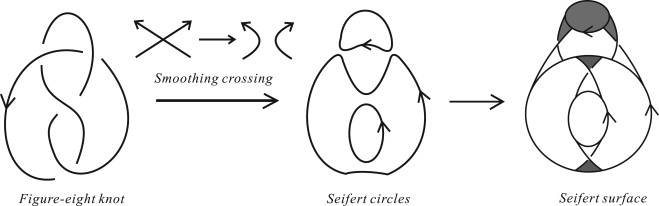
\includegraphics[width=0.75\textwidth]{../data/seifert-algorithm.jpg}
        \caption[Smthing]{Kolejne kroki algorytmu Seiferta}
    \end{figure}

    Dyski są dwustronne, więc ich górnej stronie przypisujemy znak $+$,
    jeśli tylko brzeg jest zorientowany dodatnio i~$-$ w~przeciwnym razie.
\index{algorytm!Seiferta|)}%
\end{proof}

Powierzchnia Seiferta dziedziczy orientację po węźle.
Nawet niewinne odwrócenie jednego z ogniw splotu potrafi istotnie zmienić jego powierzchnię, dlatego potrzebna jest ostrożność!

\index{powierzchnia!Seiferta|)}%

% Węzeł jest rozwłókniony dokładnie wtedy, gdy stanowi grzbiet pewnego 'open book decomposition' $S^3$.




\subsection{Węzły rozwłóknione}
\index{węzeł!rozwłókniony|(}%
Wspomnijmy jeszcze krótko o~specjalnym rodzaju węzłów i splotów.

% DICTIONARY;fibered;rozwłókniony, włóknisty;-
\begin{definition}
    Niech $L \subseteq S^3$ będzie splotem.
    Jeśli istnieje rodzina $F_t$ powierzchni Seiferta dla splotu $K$ sparametryzowana przez $t \in S^1$ taka, że $F_t \cap F_s = K$ dla $t \neq s$, to splot $K$ nazywamy rozwłóknionym albo włóknistym
\end{definition}

\index{splot!Neuwirtha}%
Dawniej nazywano je splotami Neuwirtha, gdyż ten pokazał w~swojej pracy dyplomowej z~1959 roku, że można je scharakteryzować jako sploty, których komutant grupy podstawowej jest skończenie generowany, lub równoważnie, wolny.

\begin{example}
    Niewęzeł, trójlistnik $3_1$, ósemka $4_1$, $5_{1}$, $6_{2}$, $6_{3}$, $7_{1}$, $7_{6}$, $7_{7}$, $8_{2}$, $8_{5}$, $8_{7}$, $8_{9}$, $8_{10}$, $8_{12}$, $8_{16}$..$8_{21}$, splot Hopfa oraz wszystkie węzły torusowe są rozwłóknione.
\end{example}

(Jeśli węzeł pierwszy o co najwyżej ośmiu skrzyżowaniach nie został wymieniony w tym przykładzie, to nie jest rozwłókniony).
Rozkład liczby węzłów rozwłóknionych wśród węzłów pierwszych wygląda następująco:
\begin{itemize}
\item 9 skrzyżowań -- 23 węzły,
\item 10 skrzyżowań -- 74 węzły,
\item 11 skrzyżowań -- 256 węzłów,
\item 12 skrzyżowań -- 873 węzły.
\end{itemize}
% query = 'fibered == True' + grep + nl

Lwia część analizy węzłów o 12 skrzyżowaniach została wykonana przez Stojmenowa i~Hirasawę, jak podaje baza danych KnotInfo \cite{knotinfo22}.
% źródło: https://knotinfo.math.indiana.edu/descriptions/fibered.html
\index[persons]{Hirasawa, Mikami}%
\index[persons]{Stojmenow, Aleksander}%

\begin{proposition}
\index{wielomian!Alexandera}%
    Pierwszy i~ostatni współczynnik wielomianu Alexandera węzła rozwłóknionego to $\pm 1$.
\end{proposition}

Kryterium to jest wystarczające dla węzłów pierwszych o co najwyżej 10 skrzyżowaniach oraz alternujących, ale znany jest przykład niewłóknistego węzła o 21 skrzyżowaniach, którego wielomian Alexandera ma postać $t^4 - t^3 + t^2 - t +1$.

\begin{proposition}
\index{węzeł!skręcony}%
    Niech $K$ będzie węzłem skręconym z $n$ półskrętami.
    Wtedy jego wielomianem Alexandera jest
    \begin{equation}
        \alexander_n(t) = n \cdot \left(t + \frac 1 t \right) - (2n+1),
    \end{equation}
    więc węzeł $K$ nie jest rozwłókniony, chyba że $n = 1$.
\end{proposition}

\begin{corollary}
    $2$-skręcony węzeł $6_1$ (węzeł dokerski) nie jest rozwłókniony.
\end{corollary}

Rolfsen \cite[s. 326]{rolfsen76} podaje jako ćwiczenie w swojej książce:

\begin{proposition}
    Rodzina węzłów rozwłóknionych jest zamknięta na branie sum spójnych.
\end{proposition}

\index{węzeł!rozwłókniony|)}%

% koniec podsekcji Węzły rozwłóknione




\subsection{Genus}
\index{genus|(}%
%label{sec:genus}%
Zanim przejdziemy do zdefiniowania macierzy Seiferta, potrzebować będziemy krótkiego skoku w bok -- zrozumieć bardzo geometryczny niezmiennik węzłów, genus.

Zaczniemy od starego twierdzenia, które klasyfikuje powierzchnie domknięte.

\begin{proposition}
    Każda powierzchnia domknięta jest członkiem jednej z dwóch nieskończonych rodzin:
    \begin{enumerate}[leftmargin=*]
        \itemsep0em
        \item sumą spójną $g \ge 0$ torusów,
        \item sumą spójną $k \ge 1$ rzeczywistych płaszczyzn rzutowych.
    \end{enumerate}
\end{proposition}

Elementy pierwszej rodziny są orientowalne.
Sferę traktujemy dla wygody jako sumę spójną $g = 0$ torusów.
Wtedy sumę spójną $g$ torusów możemy wyobrazić sobie jako sferę, do której doklejono $g$ uchwytów.

\begin{definition}[genus powierzchni]
    Ilość torusów nazywamy genusem powierzchni i oznaczamy literą $\genus$.
\end{definition}

Podobna charakteryzacja istnieje dla powierzchni z~brzegiem.
Każdy taki obiekt jest homeomorficzny z~sumą spójną $g$ torusów, w~których wydrążono pewną liczbę otworów: tyle, ile składowych spójności ma brzeg powierzchni.
W~przypadku powierzchni Seiferta mamy do czynienia z jednym otworem.

Dla wygody przypomnijmy jeszcze definicję klasycznego niezmiennika powierzchni:

\begin{definition}[charakterystyka Eulera]
\index{charakterystyka Eulera}%
    Niech $M$ będzie domkniętą powierzchnią orientowalną.
    Po striangulowaniu, składa się z $k_0$ wierzchołków, $k_1$ krawędzi oraz $k_2$ ścian.
    Wielkość
    \begin{equation}
        \chi = k_0 - k_1 + k_2
    \end{equation}
    jest niezmiennikiem powierzchni, zwanym charakterystyką Eulera.
\end{definition}

Definicja ta nie jest wygodna podczas ręcznych obliczeń.
Mamy za to:

\begin{proposition}
    Charakterystykę Eulera powierzchni jednoznacznie wyznaczają cztery reguły:
    \begin{itemize}
        \item jeśli $M$ jest dyskiem, to $\chi(M) = 1$,
        \item jeśli $M_1, M_2$ są powierzchniami, to $\chi(M_1 \sqcup M_2) = \chi(M_1) + \chi(M_2)$,
        \item jeśli powierzchnia $M_2$ powstaje z $M_1$ przez dołączenie paska, to $\chi(M_2) = \chi(M_1) - 1$,
        \item jeśli powierzchnia $M_2$ powstaje z $M_1$ przez dołączenie dysku do całej składowej spójności brzegu, to $\chi(M_2) = \chi(M_1) + 1$.
    \end{itemize}
\end{proposition}

Genus oraz charakterystyka Eulera są ze sobą związane:

\begin{proposition}
    Niech $M$ będzie powierzchnią o genusie $\genus$ i $\mu$ składowych spójności brzegu.
    Wtedy
    \begin{equation}
        \chi = 2 - \mu - 2\genus.
    \end{equation}
\end{proposition}

Nas interesują głównie powierzchnie Seiferta węzłów:
\index{powierzchnia Seiferta}%

\begin{proposition}
\label{prp:seifert_euler_characteristics}%
    Niech $K$ będzie węzłem z~diagramem $D$.
    Wtedy $\chi(M_D) = d - b$, gdzie $b$ jest liczbą skrzyżowań $D$, zaś $d$ jest liczbą okręgów Seiferta.
\end{proposition}

Można przeczytać o tym w \cite[s. 82]{murasugi96}.

\begin{proof}
    W~dowodzie faktu \ref{prp:seifert_exists} widzieliśmy, że liczba skrzyżowań $b$ jest jednocześnie liczbą pasków doklejonych do dysków.
    Bezpośredni rachunek pokazuje, że wtedy $k_0 = 4b$, $k_1 = 6b$ oraz $k_2 = b+d$.
    Wynika stąd, że $\chi = 4b - 6b + b + d = d - b$.
\end{proof}

Reszta tej podsekcji nie jest wymagana do zrozumienia macierzy Seiferta, przyjrzymy się genusowi jako obiektowi ciekawemu samemu w sobie.

\begin{definition}[3-genus]
    Niech $K$ będzie węzłem.
    Wśród wszystkich powierzchni Seiferta węzła $K$ istnieje co najmniej jedna o minimalnym genusie, jej genus nazywamy 3-genusem węzła $K$ i oznaczamy także przez $\genus$.
\end{definition}

Jeżeli nie powoduje to nieporozumień, zamiast 3-genus można pisać po prostu genus.

\begin{proposition}
\label{prp:genus_detects_unknot}%
    Genus wykrywa niewęzły: $K$ jest niewęzłem wtedy i tylko wtedy, gdy $g(K) = 0$.
\end{proposition}

\begin{proof}
    Niech $K$ będzie węzłem o genusie $0$.
    Z~charakteryzacji powierzchni wynika, że jego powierzchnia Seiferta to suma spójna $0$ torusów, to znaczy kula z tyloma otworami, ile $K$ ma ogniw.
    Innymi słowy, powierzchnią Seiferta węzła $K$ jest dysk, którego brzeg stanowi niewęzeł.
    To pokazuje, że implikacja w lewo jest prawdziwa.

    Implikacja w prawo jest oczywista.
\end{proof}

\subsubsection{Ograniczanie genusu z dołu}
Znalezienie 3-genusu dowolnego węzła sprawia te same trudności, co wyznaczenie jego liczby gordyjskiej.
Dowolna powierzchnia Seiferta zadaje ograniczenie z góry.
Z dołu 3-genus można szacować przy użyciu wielomianu Alexandera:
\index{wielomian!Alexandera}%

\begin{proposition}
\label{prp:alexander_genus}%
    Niech $K$ będzie węzłem.
    Wtedy $\operatorname{span} \alexander_K(t) \le 2\genus(K)$.
\end{proposition}

Fakt ten znalazłem w podręczniku Murasugiego \cite[s. 131]{murasugi96}.

\begin{proof}
    Załóżmy, że $F$ jest powierzchnią Seiferta węzła $K$ o genusie $g$.
    Wtedy macierz Seiferta powstała z $F$ jest stopnia $2g$, więc żaden ze składników jej wyznacznika nie może mieć stopnia (jako wielomian) większego niż $2g$.
\end{proof}

To dolne ograniczenie jest realizowane przez pewną powierzchnię Seiferta dla każdego pierwszego węzła o~co najwyżej 11 skrzyżowaniach poza siedmioma wyjątkami: 11n42, 11n67, 11n97 ($g = 2$), 11n34, 11n45, 11n73 oraz 11n152 ($g = 3$).
% warto byłoby dodać jakiś kod pozwalający sprawdzić, czemu akurat te węzły

\begin{proposition}
    Niech $K$ będzie węzłem, zaś $M$ jego macierzą Seiferta.
    Równość $\operatorname{span} \alexander_K(t) = 2\genus(K)$ zachodzi wtedy i tylko wtedy, gdy wyznacznik $\det M \neq 0$ jest niezerowy.
\end{proposition}

Floer zdefiniował w~\cite{floer90} przestrzeń wektorową nazywaną teraz homologią Floera, jest ona wyposażona w~endomorfizm parzystego stopnia, który powstaje z 2-wymiarowej klasy homologii reprezentowanej przez powierzchnię Seiferta.
%~kanoniczną gradację modulo $2$ oraz
\index{homologia!Floera}
Ta homologia rozkłada się na sumę prostą przestrzeni własnych wyróżnionego endomorfizmu, ich charakterystyki Eulera są współczynnikami wielomianu Alexandera.
Pozwala to na dokładniejsze szacowanie genusu węzła, patrz prace Ozsvátha, Szabó \cite{szabo03} i Ghigginiego \cite{ghiggini08}.
\index{człowiek!Ghiggini, ?}%
\index{człowiek!Ozsváth, Peter}%
\index{człowiek!Szabó, Zoltán}%

\subsubsection{Ograniczanie genusu z góry}
Z góry genus ograniczony jest przez kilka klasycznych niezmienników numerycznych.
Zanim to pokażemy, przytoczymy techniczny lemat udowodniony przez Yamadę (\cite{yamada87}):
\index{człowiek!Yamada, ?}%
% Morton MathSciNet: "The proof uses an ingenious direct algorithm to alter the projection without changing the number of Seifert circles"

\begin{proposition}
    \label{prp:seifert_circles_braid}
    Niech $L$ będzie splotem, zaś $\operatorname{s} L$ minimalną liczbą okręgów Seiferta, które dostajemy ze wszystkich możliwych diagramów splotu $L$.
    Wtedy $\operatorname{s} L = \braid L$ jest równe indeksowi warkoczowemu.
\index{indeks warkoczowy}%
\end{proposition}

Powyższe stwierdzenie występuje bez dowodu (bez?) w \cite[s. 17]{kawauchi96}.

\begin{proposition}
    Niech $L$ będzie splotem.
    Wtedy $\crossing L - \braid L - \operatorname{\mu} L + 2 \ge 2 \genus L$.
\end{proposition}

\begin{proof}
    Ustalmy minimalny diagram $D$ dla splotu $L$ i zastosujmy do niego algorytm Seiferta.
    Dostaniemy tak $s$ okręgów Seiferta oraz powierzchnię o genusie $g$.
    Fakt \ref{prp:seifert_euler_characteristics} mówiący, że $\chi = s - c$, można przekształcić do
    \begin{equation}
        g = \frac{c + 2 - s - \mu(K)}{2}.
    \end{equation}
    Z~minimalności diagramu wynika, że $c = \crossing L$.
    Fakt \ref{prp:seifert_circles_braid} mówi, że $s \ge \braid L$.
    Nierówność $g \ge \genus L$ wynika z~definicji genusu.
    Z powyższych rozważań wynika, że
    \begin{equation}
        \crossing L + 2 \ge 2 \genus L + \braid L + \operatorname{\mu} L,
    \end{equation}
    a to jest równoważnie nierówności, której prawdziwości dowodzimy.
\end{proof}

\begin{corollary}
    \label{cor:crossing_genus}
    Niech $K$ będzie węzłem.
    Wtedy $\crossing K \ge 2 \genus K$.
\index{indeks skrzyżowaniowy}
\end{corollary}

\subsubsection{Genus a rozkład na sumę węzłów pierwszych}

\begin{proposition}
    \label{prp:genus_of_sum}
    Jeśli $J, K$ są węzłami, to $g (J \shrap K) = g(J) + g(K)$.
\end{proposition}

Poniższy dowód pochodzi od Schuberta (\cite{schubert49}), został tylko zapisany we współczesnym języku.
\index{człowiek!Schubert, Horst}%
Przebiega w dwóch etapach: najpierw pokazuje się, że genus sumy nie jest większy od sumy genusów składników, a następnie, że nie jest od niej mniejszy.

\begin{proof}
    Pokażemy najpierw, że $g(J \# K) \le g(J) + g(K)$.
    Wybierzmy powierzchnie Seiferta $M_J$ oraz $M_K$ dla $J$ oraz $K$ o~minimalnym genusie.
    Suma $J \shrap K$ powstaje z~$J$ oraz $K$, podobnie jest z~powierzchniami Seiferta:
\begin{comment}
    \begin{figure}[H]
        \centering
        \begin{minipage}[b]{.48\linewidth}
        \[
            \LargeGenusProofA \longrightarrow \LargeGenusProofB
        \]
        \subcaption{suma węzłów}
        %
        \end{minipage}
        \begin{minipage}[b]{.48\linewidth}
        \[
            \LargeGenusProofC \longrightarrow \LargeGenusProofD
        \]
        \subcaption{suma powierzchni}
        \end{minipage}
    \end{figure}
\end{comment}

    Skoro $M_{J\#K}$ powstaje z~$M_J \sqcup M_K$ przez dołączenie paska do brzegu, mamy
    \begin{equation}
        \chi(M_{J\#K}) = \chi(M_J \sqcup M_K) - 1 = \chi(M_J) + \chi(M_K)-1,
    \end{equation}
    a~przez to
    \begin{equation}
        g(M_{J\#K}) = \frac{1-\chi(M_{J\#K})}{2} =
        \frac{1-\chi(M_{J})}{2} + \frac{1-\chi(M_{K})}{2}
        % = %g(M_J)+g(M_K)
        = g(J) + g(K).
    \end{equation}
    To kończy dowód pierwszej nierówności.
    Pokażemy jeszcze, że $g(J \# K) \ge g(J)+g(K)$.
    Zaczynamy od powierzchni Seiferta $M_{J\#K}$ dla $J\#K$ o~minimalnym genusie $g(M_{J\#K})$ równym $g(J\#K)$.
    Poprzez wykonanie chirurgii na powierzchni, możemy przyjąć specjalną postać jak w~poprzednim dowodzie:
\begin{comment}
    \[
        \LargeGenusProofD
    \]
\end{comment}

    Usunięcie paska daje powierzchnie Seiferta dla $M_J$ oraz $M_K$ takie, że
    \begin{equation}
        g(M_J)+g(M_K)=g(M_{J\#K})=g(J\#K).
    \end{equation}
    Oznacza to, że $g(J) + g(K) \le g(M_J) + g(M_K) = g(J\#K)$ i~mamy równość.
\end{proof}

Jesteśmy wreszcie w~stanie podać prawdziwy dowód faktu \ref{first_time_sum_is_trivial}.

\begin{corollary}
    \label{cor:connected_sum_no_inverses}
    Jeśli suma spójna dwóch węzłów jest niewęzłem, to oba składniki także nim są.
\end{corollary}

Powrócimy teraz do węzłów pierwszych.
\index{węzeł!pierwszy}%

\begin{proposition}
    Niech $K$ będzie węzłem.
    Jeśli $g(K) = 1$, to $K$ jest węzłem pierwszym.
\end{proposition}

\begin{proof}
    Załóżmy nie wprost, że węzeł $K = K_1 \# K_2$ jest sumą dwóch nietrywialnych węzłów.
    Z~faktu \ref{prp:genus_of_sum} wynika wtedy, że $g(K) = g(K_1) + g(K_2)$.
    Zatem jeden z węzłów $K_1, K_2$ ma genus zero i jest trywialny, wbrew naszemu założeniu.
\end{proof}

Implikacja odwrotna jest fałszywa: pięciolistnik jest pierwszy, ale jego genus wynosi $2$.

\begin{proposition}
    Każdy węzeł można zapisać jako suma spójna pewnej liczby węzłów pierwszych.
    Niewęzeł jest sumą pustej rodziny węzłów.
\end{proposition}

\begin{proof}
    Dowodzimy przez indukcję względem genusu $g(K)$.
    Przypadek bazowy $g(K) = 0$ jest oczywisty, gdyż wtedy $K$ to niewęzeł.
    Załóżmy więc, że fakt zachodzi dla węzłów $J$ genusu co najwyżej $n$.
    Niech $K$ będzie genusu $n + 1$.

    Jeśli $K$ jest pierwszy, nie ma czego dowodzić.
    W przeciwnym razie jest równoważny z~$J_1 \shrap J_2$, gdzie $J_1$ i~$J_2$ są nietrywialne.
    Mamy $g(J_1) + g(J_2) = g(K)$ oraz $g(J_1),g(J_2) \ge 1$.
    Zatem $g(J_1), g(J_2) \le n$.
    Na mocy hipotezy indukcyjnej, $J_1$ oraz $J_2$ są równoważne sumom
    \[
        J_1 \cong K_1\#\cdots\# K_s,\qquad
        J_2 \cong K_{s+1}\#\cdots\# K_r,
    \]
    gdzie $K_i$ są pierwsze.
    Zatem $K$ jest równoważny z~$K_1\#\cdots\# K_r$, co kończy dowód.
\end{proof}

Nasz aparat matematyczny jest niedostatecznie rozwinięty, by móc udowodnić jedyność rozkładu.

\begin{theorem}[Schubert, 1949]
    Każdy nietrywialny węzeł rozkłada się na węzły pierwsze.
    Rozkład jest, z dokładnością do kolejności składników, jednoznaczny.
\index{węzeł!pierwszy}%
\end{theorem}

Schubert podał geometryczny dowód oparty o powierzchnie Seiferta; wyraził go w języku PL-rozmaitości (\cite{schubert49}), ale niedużym wysiłkiem można dokonać adaptacji do gładkiego świata.
Praca Schuberta korzysta z twierdzenia Alexandera, że 2-sfera w przestrzeni $\R^3$ ogranicza dysk, i jego odpowiednika dla torusów w $S^3$.

Hashizume \cite{hashizume58} rozszeszył wyniki Schuberta do splotów.
% trzeba wspomnieć, że to wymaga adaptacji definicji sumy spójnej, bo wcześniej dopuszczaliśmy tylko węzły jako składniki. Remedium = Kawauchi.

\begin{proposition}
    \label{prp:infinitely_many_prime_knots}
    Istnieje nieskończenie wiele węzłów pierwszych.
\end{proposition}

\begin{proof}
    Pokażemy, że wszystkie węzły $(2n+2)_1$ są pierwsze, gdzie $n \ge 1$.
    Istotnie, algorytm Seiferta zastosowany do diagramu tego węzła wyprodukuje $2n+1$ okręgów.
\begin{comment}
    \[
        \begin{tikzpicture}[baseline=-0.65ex,scale=0.06]
        \begin{knot}[clip width=7, flip crossing/.list={1,4,5},end tolerance=1pt]
            \node at (0,10) {$\cdots$};
            \strand[semithick] (-30, -5) -- (-5, -5);
            \strand[semithick]  (5, -5) -- (30, -5);
            \strand[semithick,latex-]  (-30,-15) -- (-5,-15);
            \strand[semithick]  (5,-15) -- (30,-15);

            \strand[semithick] (-5, -15) [in=down, out=right] to (5, -10) [in=right, out=up] to (-5, -5);
            \strand[semithick] (5, -15) [in=down, out=left] to (-5, -10) [in=left, out=up] to (5, -5);

            % zewnętrzne obręcze -- lewa strona
            \strand[semithick] (-30, 15) to [out=left, in=up]   (-45, 0);
            \strand[semithick] (-30,-15) to [out=left, in=down] (-45, 0);
            \strand[semithick] (-30,  5) to [out=left, in=up]   (-35, 0);
            \strand[semithick] (-30, -5) to [out=left, in=down] (-35, 0);

            % zewnętrzne obręcze -- prawastrona
            \strand[semithick] (30, 15) to [out=right, in=up]   (45,0);
            \strand[semithick] (30,-15) to [out=right, in=down] (45,0);
            \strand[semithick] (30,  5) to [out=right, in=up]   (35,0);
            \strand[semithick] (30, -5) to [out=right, in=down] (35,0);

            % jak w~drugim ruchu Reidemeistera - górny warkocz, lewy
            \strand[semithick] (-30, 15) [in=left, out=right] to (-20,  5);
            \strand[semithick] (-30,  5) [in=left, out=right] to (-20, 15);
            \strand[semithick] (-10, 15) [in=right, out=left] to (-20,  5);
            \strand[semithick] (-10,  5) [in=right, out=left] to (-20, 15);

            % jak w~drugim ruchu Reidemeistera - górny warkocz, prawy
            \strand[semithick] (30, 15) [in=right, out=left] to (20,  5);
            \strand[semithick] (10, 15) [in=left, out=right] to (20,  5);
            \strand[semithick] (30,  5) [in=right, out=left] to (20, 15);
            \strand[semithick] (10,  5) [in=left, out=right] to (20, 15);
        \end{knot}
        \end{tikzpicture}
        \longrightarrow
        \begin{tikzpicture}[baseline=-0.65ex,scale=0.055]
            \node at (0,10) {$\cdots$};
            \draw[semithick] (-30,  -5) -- (30, -5);
            \draw[semithick] (-30, -15) -- (30,-15);

            \draw[semithick] (0,-10) circle (3);

                % zewnętrzne obręcze -- lewa strona
            \draw[semithick] (-30, 15) to [out=left, in=up]   (-45, 0);
            \draw[semithick] (-30,-15) to [out=left, in=down] (-45, 0);
            \draw[semithick] (-30,  5) to [out=left, in=up]   (-35, 0);
            \draw[semithick] (-30, -5) to [out=left, in=down] (-35, 0);

                % zewnętrzne obręcze -- prawastrona
            \draw[semithick] (30, 15) to [out=right, in=up]   (45,0);
            \draw[semithick] (30,-15) to [out=right, in=down] (45,0);
            \draw[semithick] (30,  5) to [out=right, in=up]   (35,0);
            \draw[semithick] (30, -5) to [out=right, in=down] (35,0);

            \draw[semithick] (-30, 15) to [out=right, in=up] (-20,10);
            \draw[semithick] (-30,  5) to [out=right, in=down] (-20,10);

            \draw[semithick] (30, 15) to [out=left, in=up] (20,10);
            \draw[semithick] (30,  5) to [out=left, in=down] (20,10);

            \draw[semithick] (-10, 10) circle (5);
            \draw[semithick] (10,  10) circle (5);
        \end{tikzpicture}
    \]
\end{comment}
    Wynika stąd, że genus wynosi $\frac 12 (1 - (1+2n) + (2+2n)) = 1$, ponieważ wyznacznik ma wartość $4n+1$,
    węzły $(2n+2)_1$ nie są trywialne i~są parami różne.
\end{proof}

\subsubsection{Genus kanoniczny, genus wolny}
% DICTIONARY;free;wolny;genus
% DICTIONARY;canonical;kanoniczny;genus
% DICTIONARY;genus;genus;-
Czy w definicji genusu można ograniczyć się do tych powierzchni Seiferta, które pochodzą od algorytmu Seiferta?
Niestety, poza pewnymi wyjątkami, nie.
Zanim przekonamy się, dlaczego tak jest, zdefiniujmy jeszcze dwa niezmienniki.

\begin{definition}[genus kanoniczny]
\index{genus!kanoniczny}%
    Niech $K$ będzie węzłem.
    Najmniejszy z genusów powierzchni Seiferta węzła $K$, które pochodzą z~algorytmu Seiferta, nazywamy genusem klasycznym i~oznaczamy symbolem $\operatorname{g_c} K$ lub krótko $g_c$.
\end{definition}

Stojmenow \cite{stoimenow08} opisał diagramy węzłów o~kanonicznym genusie równym 2.
Część z~jego wyników przenosi się na genus 3.
Jak sam pisze, sklasyfikowane wcześniej węzły o~genusie (kanonicznym) 1 okazały się być zbyt wąską klasą.

Pod koniec lat pięćdziesiątych Crowell i~Murasugi niezależnie zauważyli, że algorytm Seiferta zastosowany do alternującego diagramu zawsze daje powierzchnię o~minimalnej powierzchni.
Ich kombinatoryczne uzasadnienie było dość zawiłe, elementarny dowód podał Gabai w \cite{gabai86}.

Dubel trójlistnika ma genus równy $1$, ale algorytm Seiferta zastosowany wobec węzła produkuje powierzchnie o genusie co najmniej $3$, jak przewiduje ograniczenie znalezione przez Mortona w \cite[twierdzenie 2]{morton86}:

\begin{proposition}
    Niech $P(v, z)$ będzie wersją wielomianu HOMFLY spełniającą zależność
    \begin{equation}
        \frac 1v P_+ - vP_- = zP_0.
    \end{equation}
    Wtedy $M = \max \deg_z P(v, z) \le 2g_c$.
\end{proposition}

Nierówność Mortona jest równością dla wielu klas węzłów, w tym
alternujących (Crowell, Murasugi),
jednorodnych\footnote{Uogólnienie węzłów alternujących.} (Cromwell w \cite{cromwell89}),
whiteheadowskich dubli węzłów dwumostowych (Nakamura w \cite{nakamura06}, Tripp w \cite{tripp02}) albo
precli (Brittenham, Jensen \cite{brittenham06}).
\index{nierówność Mortona}%
\index{węzeł!alternujący}%
\index{węzeł!jednorodny}%
\index{dubel Whiteheada}%
\index{węzeł!dwumostowy}%
\index{precel}%
Stojmenow pokazał, że staje się równością dla węzłów o co najwyżej 12 skrzyżowaniach i znalazł przykład węzła, dla którego jest ostra.

\begin{definition}[genus wolny]
\index{ciało z rączkami}%
\index{genus!wolny}%
    Niech $K$ będzie węzłem.
    Minimalny genus spośród powierzchni Seiferta węzła $K$, których dopełnienie w 3-sferze jest ciałem z rączkami, nazywamy genusem wolnym i~oznaczamy $g_f$.
\end{definition}

Dopełnienie powierzchni Seiferta jest zawsze ciałem z rączkami, więc mamy oczywiste nierówności
\begin{equation}
    g \le g_f \le g_c.
\end{equation}
Jak duża może być różnica między kolejnymi genusami?
Już Kirby \cite[problem 1.20a]{kirby78} chciał znać oszacowania różnicy $g_f - g$.
Morton \cite{morton86} pokazał, że genus pewnych węzłów nie jest realizowany przez żaden diagram do którego stosuje się algorytm Seiferta, choćby $10_{165}$.
Moriah, matematyk izraelski, rozwiązał problem Kirby'ego dekadę później:

\begin{proposition}
    Niech $K$ będzie węzłem, $D_k(K)$ jego dublem Whiteheada z $k \neq 0$ skręceniami, zaś $B_n(K)$ to $n$-krotne nakrycie cykliczne sfery $S^3$ rozgałęzione nad węzłem $K$.
    Jeżeli ranga pierwszej grupy homologii $B_{|4k+1|}(K)$ wynosi $r$, to
    \begin{equation}
        g_f(D_k(K)) \ge \frac {2r-1} {|8k+2|}.
    \end{equation}
\end{proposition}

\begin{proof}
    Praca \cite{moriah87}.
    Dowód opiera się na chirurgii węzłów i splotów w sferze $S^3$.
\end{proof}

\begin{corollary}
    Niech $K$ bedzie sumą spójną $n$ trójlistników, połóżmy $k = -1$.
    Wtedy pierwsza grupa homologii ma rangę $r = 2n$ i~genus wolny jest nieograniczony
    \begin{equation}
        g_f(D_{-1}(3_1^n)) \ge \frac {4n-1} {6},
    \end{equation}
    podczas gdy zwykły genus to $g(D_{-1}(3_1^n)) = 1$.
\end{corollary}

Kawauchi \cite{kawauchi94} zbadał węzeł $K_m$, sumę spójną $m$ kopii skręconego whiteheadowskiego dubla trójlistnika, i policzył, że różnica $g_c(K_m) - g(K_m)$ wynosi $2m$.
Wreszcie Kobayashi oraz Kobayashi \cite{kobayashi96} wskazali nieskończoną rodzinę węzłów nieograniczonego genusu, dla której
\begin{equation}
    g_c(K) = \frac 32 g_f(K) = 2g(K).
\end{equation}
% znam ich ze Stojmenow - Knots of (canonical) genus two

\index{genus|)}

% Koniec podsekcji Genus




\subsection{Macierz Seiferta}
\index{macierz Seiferta|(}
Niech $K$ będzie węzłem z diagramem $D$ i powierzchnią Seiferta $S$.

% Murasugi, s. 79
\begin{definition}[graf Seiferta]
\index{graf Seiferta}%
    Ściągnijmy dyski z dowodu faktu \ref{prp:seifert_exists} do punktów jednocześnie kurcząc doklejone paski, otrzymamy graf zwany grafem Seiferta diagramu $D$.
\end{definition}

Murasugi \cite[s. 79]{murasugi96} proponuje jako ćwiczenie dowód faktu:

\begin{proposition}
    Graf Seiferta jest dwudzielny i planarny.
\end{proposition}

% Murasugi 82, 83
Skoro graf Seiferta jest planarny, to dzieli sferę $S^2$ na $f$ obszarów.
Można wyznaczyć ich liczbę: skoro $\chi(S^2) = d - b + f = 2$, to $f - 1 = 1 - d + b$, pomijamy obszar nieograniczony.
Brzeg każdego obszaru jest zamkniętą krzywą, z których tworzymy krzywe $x_1, \ldots, x_m$ na powierzchni Seiferta.
Generują one grupę podstawową $\pi_1(S)$.

Niech $S$ będzie powierzchnią Seiferta z wyróżnioną jedną stroną.
Jeśli krzywa $x_i$ biegnie po powierzchni $S$, przez $x_i^*$ oznaczać będziemy dodatnie wypchnięcie: krzywą równoległą do $x_i$, która biegnie tuż nad nią.
Potrzebowaliśmy wyróżnić jedną ze stron powierzchni $S$, by słowo ,,nad'' miało sens.

\begin{definition}[macierz Seiferta]
\index{macierz Seiferta}%
    Przy zachowaniu powyższych oznaczeń, macierz, której wyrazy określa wzór $M_{i,j} = \operatorname{lk}(x_i, x_j^*)$, nazywamy macierzą Seiferta.
\end{definition}

Konstrukcja macierzy Seiferta zależy od wyboru diagramu oraz orientacji krzywych $x_i$, dlatego nie jest niezmiennikiem węzłów.
Stanie się nim, kiedy uwzględnimy jeszcze wpływ ruchów Reidemeistera.

\begin{proposition}
    Kwadratowa macierz $V$ o całkowitych wyrazach jest macierzą Seiferta węzła wtedy i~tylko wtedy, gdy $\det(V - V^t) = 1$.
\end{proposition}

\begin{proof}
    Kawauchi \cite[s. 62]{kawauchi96} pisze, że wynika to z~klasyfikacji macierzy Seiferta splotów.
\end{proof}

\begin{definition}
    Operacja $\Lambda_1$ dla pewnej odwracalnej macierzy $P$ o całkowitych wyrazach (czyli $\det P = \pm 1$) to
    \begin{equation}
        \Lambda_1 \colon M \mapsto PMP^t.
    \end{equation}
    Natomiast operację $\Lambda_2$ definiuje wzór:
    \begin{equation}
        \Lambda_2 \colon M \mapsto \begin{bmatrix}
  &   &  & 0 & 0 \\
  & M &  & \vdots & \vdots \\
  &   &  & 0 & 0 \\
* & \dots & * & 0 & 0 \\
0 & \dots & 0 & 1 & 0
\end{bmatrix} \textrm{albo} \begin{bmatrix}
  &   &  & * & 0 \\
  & M &  & \vdots & \vdots \\
  &   &  & * & 0 \\
0 & \dots & 0 & 0 & 1 \\
0 & \dots & 0 & 0 & 0
\end{bmatrix},
    \end{equation}
    gdzie gwiazdka zastępuje ustaloną liczbę całkowitą.
\end{definition}

\begin{definition}
\index{macierz Seiferta!S-równoważność}%
\index{S-równoważność (macierzy Seiferta)}%
    Niech $M_1, M_2$ będą macierzami.
    Jeśli $M_2$ można otrzymać z $M_1$ przez skończony ciąg operacji $\Lambda_1, \Lambda_2$ oraz ich odwrotności, to macierze nazywamy $S$-równoważnymi.
\end{definition}

Badania powyższej relacji równoważności prowadzili w~latach sześćdziesiątych ubiegłego stulecia Trotter \cite{trotter62}, Murasugi \cite{murasugi65} oraz Levine \cite{levine70}.
\index[persons]{Trotter, Hale}%
\index[persons]{Murasugi, Kunio}%
\index[persons]{Levine, Jerome}%
Litera $S$, jak nietrudno się domyślić, pochodzi od Seiferta.

\begin{proposition}
    Macierz Seiferta modulo $S$-równoważność jest niezmiennikiem splotów.
\end{proposition}

Dowód tego faktu jest elementarny, ale dość długi.
Razem z~ułatwiającymi zrozumienie diagramami można znaleźć go w podręczniku Kawauchiego \cite[s. 64]{kawauchi96} albo Murasugiego, dlatego pomijamy go i skupimy się na tym, jakie niezmienniki można otrzymać z macierzy Seiferta.

Wyznacznik całej macierzy Seiferta nie jest niezmiennikiem.
Wykonując operację $\Lambda_2$ dostajemy macierz, której ostatnia kolumna albo ostatni wiersz są zerami, więc jej wyznacznik także jest zerem.
Jeśli jednak najpierw dokonamy jej symetryzacji, dostaniemy znany już niezmiennik.

\begin{proposition}
\index{wyznacznik}%
    Niech $M$ będzie macierzą Seiferta węzła $K$.
    Wtedy
    \begin{equation}
        \det K = |\det(M + M^t)|.
    \end{equation}
\end{proposition}

\index{wielomian!Alexandera}%
Przez wprowadzenie dodatkowej zmiennej $t \in \R$, ponownie uogólnimy wyznacznik do wielomianu Alexandera.

\begin{proposition}
    Niech $M$ będzie macierzą Seiferta stopnia $k$ węzła $K$.
    Wtedy
    \begin{equation}
        \alexander_K (t) = t^{-k/2}\det(M - tM^t).
    \end{equation}
\end{proposition}

Określimy jeszcze dwa, niewystępujący wcześniej niezmiennik (Arfa i sygnaturę).

\index{macierz Seiferta|)}




\subsection{Sygnatura}
\label{sub:signature}%
\index{sygnatura|(}%
Sygnatura jest kolejnym niezmiennikiem, do zdefiniowania których wystarczy znać macierz Seiferta.
Pochodzi prawdopodobnie z lat sześćdziesiątych (Trotter \cite{trotter1962} dla węzłów, Murasugi \cite{murasugi1965} dla splotów).
\index[persons]{Trotter, Hale}%
\index[persons]{Murasugi, Kunio}%
% z recenzji do 275415: Shinohara, Yaichi - On the signature of knots and links.
Ktoś powiedział nam kiedyś, że ujednolicenia różnych podejść do form kwadratowych związanych z węzłami dokonali Gordon, Litherland, Murasugi w~pracy \cite{litherland1981}, ale potem trafiliśmy na artykuł Przytyckiego \cite{przytycki2011} pełen historycznych ciekawostek oraz dwóch kolejnych odnośników: do wspomnianej przed chwilą pracy \cite{murasugi1965}, ale też \cite{gordon1978} samych Gordona, Litherlanda, którzy sięgają zenitu i wiążą dziełą Goeritza, Trottera, Murasugiego et alli.
Może po prostu najlepiej przeczytać wszystko?

% DICTIONARY;signature;sygnatura;-
\begin{definition}[sygnatura]
\label{def:signature}%
    Niech $M$ będzie macierzą Seiferta zorientowanego splotu $L$.
    Wielkość
    \begin{equation}
        \sigma_L := \operatorname{\sigma} (M + M^t),
    \end{equation}
    sygnaturę macierzy $M + M^t$, nazywamy sygnaturą splotu $L$.
\end{definition}

\begin{proposition}
\label{prp:signature_additive}%
    Sygnatura jest addytywna: $\sigma(K_1 \shrap \ldots \shrap K_n) = \sum_{k=1}^n \sigma(K_k)$.
\end{proposition}

Wiem o tym z \cite[s. 127]{murasugi1996}.

\begin{proof}
    Bez straty ogólności ograniczmy się do przypadku $n = 2$ i~ustalmy powierzchnie Seiferta $F_1, F_2$ dla węzłów $K_1, K_2$ z~macierzami Seiferta $M_1, M_2$.
    Powierzchnia dla ich sumy spójnej $K_1 \shrap K_2$ powstaje przez sklejenie $F_1$ oraz $F_2$ paskiem.
    W języku macierzy oznacza to, że macierz Seiferta węzła $K_1 \shrap K_2$ ma postać $M = M_1 \oplus M_2$.
    Zatem:
    \begin{align}
        \sigma(K_1 \shrap K_2) & = \sigma(M + M^t) \\
                               & = \sigma(M_1 + M_1^t) + \sigma(M_2 + M_2^t) \\
                               & = \sigma(K_1) + \sigma(K_2),
    \end{align}
    co kończy dowód.
\end{proof}

\begin{corollary}
\index{liczba mostowa}%
\label{no_relation_signature_bridge}%
    Nie istnieje bezpośredni związek między sygnaturą i~liczbą mostową.
\end{corollary}

Wiemy o tym z książki Livingstona \cite[s. 145]{livingston1993}.

\begin{proof}
    Węzeł torusowy $T_{2,n}$ jest dwumostowy, jego sygnatura wynosi $n - 1$.
    Suma spójna węzłów prostych (sumy przeciwnie zorientowanych trójlistników) ma zerową sygnaturę, ale na mocy faktu~\ref{prp:bridge_additive} jej liczba mostowa jest nieograniczona.
\end{proof}

\begin{proposition}
\index{lustro}%
\index{rewers}%
\label{prp:signature_mirror_reverse}%
    Niech $L$ będzie splotem.
    Wtedy $\sigma(mL) = -\sigma(L)$ oraz $\sigma(rL) = \sigma(L)$.
\end{proposition}

O tym także wiem z \cite[s. 127]{murasugi1996}.

\begin{proof}
    Wynika to z podobnych faktów dla macierzy Seiferta.
    Równoważność $M_{mL} \simeq - M_L^t$ wynika z tego, że zamiana nad- i podskrzyżowań odwraca wzajemne położenie krzywych, których indeksu zaczepienia szukamy.

    Podobnie pokazuje się, że $M_{rL} \simeq M_L^t$.
\end{proof}

\begin{corollary}
\index{węzeł!achiralny}%
\label{cor:acheiral_signature}%
    Jeśli $K$ jest węzłem achiralnym, to $\sigma(K) = 0$.
\end{corollary}

Węzły achiralne mają zerową sygnaturę, zatem trójlistnik nie jest achiralny.
Z faktów~\ref{prp:signature_additive} oraz~\ref{prp:signature_mirror_reverse} wynika, że suma tak samo zorientowanych trójlistników nie jest achiralna ($\sigma = \pm 4$).
Jak można przekonać się ze standardowego diagramu węzła prostego, ten jest achiralny.
Pisaliśmy coś o tym na stronie \pageref{two_sums_of_two_trefoils}.

\begin{proposition}
\label{trivial_alexander_polynomial}%
\index{wielomian!Alexandera}%
    Niech $K$ będzie węzłem.
    Jeśli $\alexander_K(t) \equiv 1$, to $\sigma (K) = 0$.
\end{proposition}

Założenie $\alexander_K(t) \equiv 1$ jest spełnione przez cztery węzły pierwsze do 12 skrzyżowań, są to $11n_{34}, 11n_{42}, 12n_{313}$ oraz $12n_{430}$, patrz wzmianka po fakcie~\ref{alexander_no_detects_unknot}.
% ZWERYFIKOWANO: funkcja trivial_alexander

\begin{proof}
\index[persons]{Milnor, John}%
    Murasugi twierdzi, że zostało to udowodnione przez Milnora w \cite{milnor1968}, nie jesteśmy jednak pewni, gdzie dokładnie, ale raczej poza sekcją piątą.
\end{proof}

Istnieje równoważna definicja, która nie wymaga czasochłonnego wyznaczania macierzy Seiferta.

\begin{proposition}
\index{relacja kłębiasta}%
    Sygnatura to niezmiennik topologiczny zadany kłębiastą relacją rekurencyjną:
    \begin{itemize}[leftmargin=*]
    \itemsep0em
        \item $\sigma (\SmallUnknot) = 0$,
        \item $\sigma (K_+) - \sigma (K_-) \in \{0, 2\}$,
        \item $4 \mid \sigma (K)$ wtedy i~tylko wtedy, gdy $\conway(2i) > 0$ (wielomian Conwaya).
    \end{itemize}
\end{proposition}

Symbole $K_+, K_-$ objaśnione są przy definicji~\ref{skein_symbols}.

\begin{proof}
    Wystarczy pokazać, że sygnatura węzła spełnia trzy powyższe aksjomaty, a~następnie zauważyć, że korzystając z~nich jesteśmy w~stanie wyznaczyć jednoznacznie sygnaturę dla dowolnego węzła.
    Wynika to z~faktu, że każdy węzeł można zmienić w~niewęzeł odwracając pewne skrzyżowania.
    Pomysł opisał dokładnie Giller \cite[trzecie spostrzeżenie]{giller1982}, sam oparł się o~\cite[twierdzenie 5.6]{murasugi1965}.
\index[persons]{Giller, Cole}%
\end{proof}

Sygnatura pozwala uzyskać proste oszacowanie liczby gordyjskiej od dołu:
\index{liczba gordyjska}%

\begin{proposition}
    Mamy $2 u(K) \ge |\sigma(K)|$.
\end{proposition}

Liczba gordyjska 83 z~801 węzłów pierwszych o mniej niż dwunastu skrzyżowaniach nie jest jeszcze znana.
Dla 272 spośród pozostałych mamy równość $2u = |\sigma|$.
% ZWERYFIKOWANO: funkcja unknotting_sigma 

\begin{proof}
    Ustalmy diagram $D$ dla węzła $K$.
    Odwrócenie dowolnego skrzyżowania polega na przejściu z~diagramu $D_+$ do $D_-$ lub z~$D_-$ do $D_+$.
    Zgodnie z relacją kłębiastą, sygnatura pozostaje taka sama lub zmienia wartość o $2$.
    Po wykonaniu $u$ odwróceń otrzymujemy diagram niewęzła o~sygnaturze zero, zatem sygnatura wyjściowego węzła nie mogła przekraczać $2u$.
    To kończy dowód.
\end{proof}

W~\cite{shinohara1971} Shinohara pokazał, że dla każdej pary nieujemnych liczb całkowitych $m, n$ istnieje węzeł $K$ o wyznaczniku $4m+1$ ($8m+5$, $4m+3$) oraz sygnaturze bez znaku $8n$ ($8n+4$, $4n+2$).
\index[persons]{Shinohara, Yaichi}%
\index{wyznacznik}%
Ponadto, jeśli $m$ nie dzieli się przez $3$, istnieje węzeł o wyznaczniku $8m+1$ i sygnaturze bez znaku $8n+4$.
% skąd to? Ohtsuki?

Czas na raczej niezbyt użyteczną ciekawostkę.

\begin{conjecture}
    Czy istnieje węzeł o~sygnaturze $4$ i~wyznaczniku postaci $n = 4k + 1$?
\end{conjecture}

Stojmenow twierdzi, że jeśli tak jest, to wszystkie pierwsze dzielniki $n$ dają resztę $1$ z~dzielenia przez $24$ i~są większe od $2857$.
\index[persons]{Stojmenow, Aleksander}%
Patrz \cite[s. 540]{ohtsuki2002}.

Czytając przeglądową pracę Conwaya \cite{conway2019} dowiedzieliśmy się, że w~latach sześćdziesiątych sygnatura została uogólniona do funkcji $\sigma_L \colon S^1 \to \Z$.
\index[persons]{Conway, John}%
Większość podręczników, a także prace Levine'a \cite{levine1969} oraz Tristrama \cite{tristram1969}, wprowadza ją przy użyciu macierzy Seiferta, więc my postąpimy dokładnie tak samo.
\index[persons]{Levine, Jerome}%
\index[persons]{Tristram, Andrew}%

\begin{definition}[sygnatura Levine'a-Tristrama]
\index{sygnatura!Levine'a-Tristrama}%
    Niech $M$ będzie macierzą Seiferta zorientowanego splotu $L$.
    Funkcję $\sigma_L \colon S^1 \to \Z$ daną wzorem
    \begin{equation}
        \sigma_L(\omega) := \operatorname{\sigma} [(1-\omega) M + (1 - \overline{\omega})M^t]
    \end{equation}
    nazywamy sygnaturą Levine'a-Tristrama splotu $L$.
    Jest niezmiennikiem splotów.
\end{definition}

Funkcja $\sigma_L$ jest kawałkami stała.
Conway pisze w \cite{conway2019}, że wynika to ze wzoru na wielomian Alexandera $\Delta_L(t) = \det(tM - M^t)$.
\index[persons]{Conway, John}%
\index{wielomian!Alexandera}%
Jedynymi punktami nieciągłości są zera wielomianu $(t-1)\Delta_L(t)$, to świeży wynik Gilmera, Livingstona z~\cite{gilmer2016}.
\index[persons]{Gilmer, Patrick}%
\index[persons]{Livingston, Charles}%

Mówimy, że funkcja zdefiniowana na okręgu jest zbalansowana, jeżeli w każdym punkcie nieciągłości przyjmuje wartość równą średniej z~lewo- oraz prawostronnej granicy w tym punkcie.
Livingston podał pełną charakteryzację zbilansowanych sygnatur Levine'a-Tristrama dla węzłów, analogiczny problem dla splotów wydaje się być wciąż otwarty.

\begin{proposition}
\label{balanced_iff_four_conditions}%
    Funkcja zbalansowana $\sigma \colon S^1 \to \Z$ jest realizowana jako sygnatura pewnego węzła wtedy i tylko wtedy, gdy:
    \begin{enumerate}
        \item dla każdego $\omega \in S^1$ mamy $\sigma(\omega) = \sigma(\overline{\omega})$
        \item $\sigma(1) = 0$
        \item każdy punkt nieciągłości funkcji $\sigma$ jest miejscem zerowym wielomianu Alexandera węzła
        \item jeżeli argumenty $\omega_1, \omega_2$ są sprzężone w sensie Galois, to $\sigma(\omega_1) \equiv \sigma(\omega_2)$ modulo $2$.
    \end{enumerate}
\end{proposition}

\begin{proof}
    Livingston pisze w \cite{livingston2018}, że dowód w prawą stronę jest dość dobrze znany, natomiast w lewo korzysta z~wyników Kondo \cite{kondo1979} i Sakaiego \cite{sakai1977}, że każdy wielomian Alexandera węzła jest realizowany przez węzeł 1-gordyjski oraz zachowania zbalansowanej sygnatury podczas odwracania skrzyżowania.
\end{proof}

Kawauchi \cite[s. 151]{kawauchi1996} wspomina nierówność $\unknotting K \ge \log_3 |Q(-1)|$.
Węzeł $8_{18}$ jest 2-gordyjski i jego wielomian BLM/Ho wynosi
\begin{equation}
    Q (8_{18}; x) = 6x^7 + 24x^6 + 14x^5 - 36x^4 - 26x^3 + 12x^2 + 2x + 5,
\end{equation}
więc $Q (8_{18}, -1) = 9$ i żaden 1-gordyjski węzeł nie może mieć tego samego wielomianu BLM/Ho, a na mocy także takiego samego wielomianu Kauffmana jak $8_{18}$.
(Dokładnie to samo rozumowanie działa dla $9_{35}, 9_{37}, 9_{46}, 9_{47}, 9_{48}, 10_{74}, 10_{75}, 10_{98}, 10_{99}$, 31 węzłów pierwszych o 11 skrzyżowaniach i 123 węzłów pierwszych o 12 skrzyżowaniach).
% TODO: tu? czy bliżej 1-gordyjskich?
% TODO: dopisać pythonowy program
% 8_18 9_35 9_37 9_46 9_47 9_48 10_74 10_75 10_98 10_99 11a_43 11a_44 11a_47 11a_57 11a_123 11a_135 11a_155 11a_173 11a_181 11a_231 11a_249 11a_263 11a_277 11a_291 11a_293 11a_314 11a_332 11a_352 11a_366 11n_71 11n_72 11n_73 11n_74 11n_75 11n_76 11n_77 11n_78 11n_81 11n_126 11n_164 11n_167 12a_119 12a_164 12a_166 12a_167 12a_177 12a_244 12a_245 12a_265 12a_270 12a_295 12a_297 12a_298 12a_311 12a_332 12a_386 12a_396 12a_413 12a_427 12a_433 12a_435 12a_493 12a_503 12a_554 12a_563 12a_569 12a_574 12a_576 12a_594 12a_615 12a_634 12a_647 12a_679 12a_683 12a_692 12a_701 12a_712 12a_725 12a_742 12a_750 12a_769 12a_787 12a_801 12a_810 12a_873 12a_886 12a_895 12a_905 12a_973 12a_987 12a_990 12a_1022 12a_1092 12a_1093 12a_1123 12a_1142 12a_1181 12a_1225 12a_1260 12a_1283 12a_1286 12a_1288 12n_268 12n_269 12n_270 12n_332 12n_333 12n_334 12n_379 12n_380 12n_386 12n_387 12n_388 12n_389 12n_402 12n_403 12n_420 12n_440 12n_460 12n_480 12n_494 12n_495 12n_496 12n_505 12n_508 12n_518 12n_546 12n_549 12n_553 12n_554 12n_555 12n_556 12n_565 12n_567 12n_570 12n_571 12n_574 12n_581 12n_582 12n_583 12n_598 12n_600 12n_601 12n_602 12n_604 12n_605 12n_622 12n_626 12n_636 12n_637 12n_642 12n_654 12n_666 12n_669 12n_701 12n_737 12n_756 12n_806 12n_813 12n_846 12n_869 12n_876 12n_883 12n_888

\begin{proposition}
\index{węzeł!satelitarny}%
    Niech $S$ będzie satelitą z towarzyszem $C$, wzorcem $P$ oraz indeksem zaczepenia $n$.
    Wtedy
    \begin{equation}
        \sigma_S(\omega) = \sigma_P(\omega) + \sigma_C(\omega^n).
    \end{equation}
\end{proposition}

\begin{proof}
    Szczególny przypadek $\omega = -1$ rozpatrywał wcześniej Shinohara w~\cite{shinohara1971}.
\index[persons]{Shinohara, Yaichi}%
    Pełny dowód znajduje się w artykule \cite{litherland1979} Litherlanda.
\index[persons]{Litherland, Richard}%
\end{proof}

Wreszcie:

\begin{proposition}
    Niech $L$ będzie splotem.
    Wtedy albo wielomian Alexandera $\Delta_L(t)$ jest tożsamościowo zerem, albo posiada co najmniej $|\sigma_L|$ zer, liczonych z krotnościami, na okręgu jednostkowym.
\end{proposition}

\begin{proof}
    Aneks w książce Liechtiego \cite{liechti2016}, która nie wygląda na związaną z~teorią węzłów.
\end{proof}

\index{sygnatura|)}%

% Koniec podsekcji Sygnatura



% koniec sekcji macierz Seiferta

\section{Niezmiennik Arfa}
\index{niezmiennik!Arfa|(}%

Cahit Arf wprowadził w 1941 roku pewien niezmiennik nieosobliwych form kwadratowych nad ciałem charakterystyki dwu.
\index[persons]{Arf, Cahit}%
Zrobił to między innymi po to, by sklasyfikować takie formy kwadratowe.
My poznamy wariant niezmiennika Arfy dla węzłów.

Niech $(v_{i,j})$ będzie macierzą Seiferta węzła $K$ o genusie $g$.
Wtedy jej wymiary wynoszą $2g \times 2g$ i macierz $V-V^t$ jest symplektyczna.

\begin{definition}
    Zachowując powyższe oznaczenia, niezmiennik Arfa to
    \begin{equation}
        \sum^g_{i=1}v_{2i-1,2i-1}v_{2i,2i} \pmod 2.
    \end{equation}
    % Przyjmuje on dwie wartości: 0, 1
\end{definition}

Niezmiennik Arfa dla węzłów można zdefiniować na kilka sposobów, z~których żaden nie jest istotnie lepszy od pozostałych.
Pierwszy był pomysł Robertello \cite{robertello65}:
\index[persons]{Robertello, Raymond}%

\begin{proposition}[Robertello, 1965]
    Niech $K$ będzie węzłem, zaś
    \begin{equation}
        \alexander_K(t)=c_{0}+c_{1}t+\cdots +c_{n}t^{n}+\cdots +c_{0}t^{2n}
    \end{equation}
    jego wielomianem Alexandera.
    Wtedy niezmiennik Arfa to $c_{n-1}+c_{n-3}+\cdots +c_{r} \mod 2$, gdzie $r = 0$ dla nieparzystych $n$, $r = 1$ w~przeciwnym razie.
\end{proposition}

Nieco później Murasugi \cite{murasugi69} zauważył, że warunek można uprościć:
\index[persons]{Murasugi, Kunio}%

\begin{proposition}[Murasugi, 1969]
    \label{prp:arf_murasugi}
    Niech $K$ będzie węzłem.
    Wtedy $\operatorname{Arf} K = 0$ wtedy i~tylko wtedy, gdy $\alexander_K(-1) \equiv \pm 1 \mod 8$.
\end{proposition}

Kauffman zaproponował trochę inne podejście z wykorzystaniem diagramów.
\index[persons]{Kauffman, Louis}%
Dwa węzły nazwiemy równoważnymi przez przejścia, jeśli są związane skończenie wieloma ,,przejściami'' \cite[s. 143]{kauffman83}:
\begin{comment}
\[
    \LargeTwoPassMoveA \cong \LargeTwoPassMoveB
    \quad\mbox{albo}\quad
    \LargeTwoPassMoveC \cong \LargeTwoPassMoveD
\]
\end{comment}

\begin{definition}[Kauffman, 1983]
    Każdy węzeł $K$ jest równoważny przez przejścia albo z niewęzłem (wtedy mówimy, że $\operatorname{Arf} K = 0$), albo z trójlistnikiem (wtedy, że $\operatorname{Arf} K = 1$).
\end{definition}

Wreszcie Jones zauważył \cite[tw. 19]{jones85}, że dzięki zespolonym algebrom Clifforda oraz pracy \cite{lannes85} niezmiennik Arfa jest specjalną wartością wielomianu Jonesa.
Jest to jedyna definicja, którą łatwo rozszerzyć do splotów.

\begin{proposition}[Jones, 1985]
\label{prp:arf_jones}%
    $\operatorname{Arf}(K) = \jones_K(i)$.
\end{proposition}

\begin{corollary}
    Niezmiennik Arfa jest $\shrap$-addytywny (modulo 2).
\end{corollary}

\begin{proof}
    Wynika to z faktu \ref{prp:arf_jones} oraz \ref{prp:jones_multiplicative_2}, ale bezpośredni dowód też istnieje. % gdzie?
\end{proof}

O niezmienniku Arfa usłyszymy jeszcze poznając węzły plastrowe.

\index{niezmiennik!Arfa|)}

% Koniec sekcji Niezmiennik Arfa


\section{Homologie}

Ta sekcja wymaga znajomości przynajmniej homologii: kompleksów łańcuchowych, różniczek, grup homologii.
Można się tego nauczyć z~każdego podręcznika topologii algebraicznej.

\subsection{Homologie Chowanowa}
\index{homologia!Chowanowa|(}
Viro napisał w 2004 piękną pracę \cite{viro04}, by objaśnić homologię Chowanowa używając tak mało algebry, jak to tylko możliwe.
Jest przyjazna dla początkujących, więc na niej opiera się reszta tej podsekcji\footnote{Viro wymienia kilka innych artykułów, z których można czerpać wiedzę. \emph{,,A good place to start: \cite{barnatan02} followed by \cite{shumakovitch12}, \cite{khovanov00}. Another possible starting point: \cite{turner17}.''}}.
Będziemy pracować ze stanami Kauffmana i obramowanymi węzłami, ponieważ autor sugeruje, że to bardziej naturalne.
Oryginalna praca Chowanowa to \cite{khovanov00}.

Niech $L$ będzie splotem, zaś $D$ jego diagramem.
Chowanow skonstruował rodzinę grup $\mathcal H^{i, j}(D)$ takich, że
\begin{equation}
    K(L, q) = \sum_{i, j} q^j (-1)^i \dim_\Q (\mathcal H^{i, j}(D) \otimes \Q),
\end{equation}
gdzie $K$ jest wersją wielomianu Jonesa.
Grupy $\mathcal H^{i, j}$ są u~niego grupami homologii pewnych kompleksów łańcuchowych.
Ich konstrukcja była przeładowana algebraicznymi szczegółami, później Bar-Natan \cite{barnatan02}, Viro podali jej warianty z~myślą o~topologach.
% Viro - Remarks on definition of Khovanov homology, arXiv

Homologię Chowanowa nazywa się kategoryfikacją wielomianu Jonesa.
Zanim zagłębimy się w szczegóły, rozpatrzmy prostszy przykład tego procesu.
Niech $X$ będzie przestrzenią topologiczną, wtedy charakterystykę Eulera oraz grupy homologii łączy zależność
\begin{equation}
    \chi(X) = \sum_{n = 0}^{\dim X} (-1)^n \operatorname{rk} H_n(X),
\end{equation}
a przy tym grupy homologii dostarczają więcej informacji, co więcej można o nich myśleć jako funktorach.
Homologie są kategoryfikacją charakterystyki Eulera.

Kategoryfikacja wielomianu Jonesa polega na zastąpieniu jakoś jego współczynników przez ciąg grup abelowych.
Wzór o sumowaniu stanów przypomina ostatnią równość, brakuje tylko przedstawienia składników po prawej stronie jako alternująca suma rang grup.

Viro zauważa, że powszechna definicja wielomianu Jonesa sprawia problem dla pustego splotu (którego nigdy wcześniej nie rozpatrywaliśmy).
Mamy:
\begin{equation}
    \jones_\varnothing = \frac{1}{-t^{1/2} - t^{-1/2}},
\end{equation}
a to nie jest wielomian Laurenta jednej zmiennej.
\index{wielomian Jonesa!powiększony}%
Dlatego definiuje powiększony wielomian Jonesa:
\begin{equation}
    \widetilde{\jones_L}(t) = (-t^{1/2} - t^{-1/2}) \cdot \jones_L(t),
\end{equation}
i mówi, że będzie kategoryfikować powiększony wielomian Jonesa, a właściwie powiększoną klamrę Kauffmana.

Jak pisze dalej, pewne drobne trudności techniczne mogły skłonić Chowanowa do pozbycia się ułamkowych potęg przez zmianę zmiennej w~powiększonym wielomianie Jonesa: niech $q := -t^{1/2}$.
Dostaje się tak nowy wielomian, nazwijmy go $K$.
Spełnia trzy aksjomaty:
\begin{itemize}
\item (normalizacja) $K(\SmallUnknot) = q + 1/q$;
\item (stabilizacja) $K(L \sqcup \SmallUnknot) = (q + 1/q) K(L)$;
\item (relacja kłębiasta) \begin{equation}
    q^{-2}     K\left( \MediumPlusCrossingArrows \right) -
    q^{2}      K\left( \MediumMinusCrossingArrows \right) =
    (q^{-1}-q) K\left( \MediumJustSmoothing \right).
\end{equation}
\end{itemize}

Stąd widać już, jakie grupy dobrać dla niewęzła:
\begin{equation}
    H^{i,j} = \begin{cases}
        \Z & \textrm{ jeśli } i = 0, j = \pm 1 \\
        0  & \textrm{ w przeciwnym razie}.
    \end{cases}
\end{equation}
Wtedy spełniona jest równość
\begin{equation}
    K(L, q) = \sum_{i, j} (-1)^i q^j \operatorname{rk} H^{i, j} (L).
\end{equation}
Pozostało powtórzyć to dla dowolnego splotu.
Wzór o sumowaniu stanów przybiera postać:
\begin{equation}
    K(L, q) = \sum_s (-1)^{(\writhe D - |s|)/2} q^{(3\writhe D - |s|)/2} (q+1/q)^{|sD|}.
\end{equation}

Reprezentacja ta ma jedną wadę: każdy składnik z prawej strony przyczynia się do różnych jednomianów, zatem ma wpływ na różne grupy (których dopiero szukamy).
,,Surowe'' stany nie są prawdziwym odpowiednikiem sympleksów, jakie spotyka się podczas kategoryfikacji charakterystyki Eulera.
Najprostszym pomysłem, jak to naprawić, jest rozbicie ostatniej potęgi $q + 1/q$.
Zauważmy, że ma tyle czynników, ile wygładzenie diagramu ma składowych.
To motywuje definicję:

\begin{definition}[stan wzbogacony]
\index{stan!wzbogacony}%
    Stan diagramu $D$ razem z przypisaniem znaku $+$ lub $-$ do każdego okręgu $sD$ nazywamy stanem wzbogaconym.
\end{definition}

Dla ustalonego wzbogaconego stanu $S$ diagramu $D$ oznaczmy przez $\tau(S)$ sumę znaków przypisanych do okręgów\footnote{Oznaczenie wzięte z pracy Viro, żywimy nadzieję, że nikt nie weźmie $\tau$ za liczbę kolorowań z rodziału drugiego. Poza tym, Viro pisze $\sigma(s)$ zamiast naszego $|s|$ oraz $|s|$ zamiast naszego $|sD|$. Ostrożność wskazana.}.
Wtedy
\begin{equation}
    q^{(3 \writhe D - |s|)/2} (q + 1/q)^{|sD|} = \sum_{S/s} q^{(3 \writhe D - |s| + 2 \tau(S))/2},
\end{equation}
gdzie sumowanie odbywa się po wszystkich stanach $S$ wzbogacających stan $s$.
Niech
\begin{equation}
    j(S) := \frac 12 (3 \writhe D - |s| + 2 \tau(S)).
\end{equation}
Dobrnęliśmy do
\begin{equation}
    K(L, q) = \sum_S (-1)^{(\writhe D - |s|)/2} q^{j(S)},
\end{equation}
tym razem sumujemy po wszystkich wzbogaconych stanach diagramu $D$.

Potrzebujemy jeszcze trochę nowych obiektów.
Niech $C(D)$ oznacza wolną abelową grupę generowaną przez wzbogacone stany diagramu $D$, a $C^j(D)$ będzie jej podgrupą generowaną przez wzbogacone stany $S$ takie, że $j(S) = j$.

Czyni to $C(D)$ wolną grupą abelową z $\Z$-gradacją:
\begin{equation}
    C(D) = \bigoplus_{j \in \Z} C^j (D).
\end{equation}

Dla ustalonego stanu wzbogaconego $S$, niech $i(S) = (\writhe D - |s|)/2$.
Określmy ostatnią podgrupę, $C^{i,j}(D) \le C^j(S)$ generowaną przez wzbudzone stany $S$, dla których $i(S) = i$.
Dostajemy wreszcie
\begin{equation}
    K(L, q) = \sum_{j = -\infty}^\infty q^j \sum_{i = -\infty}^\infty (-1)^i \operatorname{rk} C^{i, j}(D).
\end{equation}

Teraz ,,wystarczy'' zdefiniować funkcję $d$ i sprawdzić, że jest różniczką, to znaczy że $d^2 = 0$.
Tak też robi Viro, nam brakuje sił, by przybliżyć konstrukcję.
To już koniec -- różniczka pozwala przejść z grup $C^{i,j}$ do grup homologii.
Pewne wyjaśnienia znaleźć można w~\cite[s. 42]{przytycki15}, gdzie podano przepis wymagający właściwie tylko ponumerowania skrzyżowań.

Bar-Natan, topolog izraelski, napisał program liczący homologie Chowanowa szybko \cite{barnatan07}, przy czym szybko oznacza: chyba\footnote{Źródło: komentarze pod postem \url{https://mathoverflow.net/a/232267}} w~czasie $O(\exp(c \sqrt n))$, dla diagramu o~$n$ skrzyżowaniach.
Nie możemy liczyć na istotne przyspieszenie:
znalezienie przybliżenia wielomianu Jonesa jest problemem \#P-trudnym (\cite{kuperberg15}, \cite{vertigan05}),
a przy znanych homologiach -- trywialnym.
(Ale patrz też fakt \ref{prp:jones_at_roots_of_unity}).

Kronheimer, Mrówka \cite{kronheimer11} pokazali:

\begin{proposition}
\label{khovanov_detects_unknot}%
    Zredukowana kohomologia Chowanowa wykrywa niewęzeł.
\end{proposition}

\begin{proof}
    Dowód składa się z dwóch kroków.
    W pierwszym panowie pokazują, że istnieje ciąg spektralny zaczynający się od zredukowanej kohomologii Chowanowa, po którym następuje koniec: homologia zdefiniowana osobliwymi instantonami.

% DICTIONARY;sutured manifold;rozmaitość szwowa;-
\index{rozmaitość szwowa}
    Potem dowodzą, że ta homologia jest izomorficzna z instantonową homologią Floera szwowego dopełnienia węzła, o której wiadomo, że wykrywa niewęzeł.
\end{proof}

\index{homologia!Chowanowa|)}

\subsection{Homologia Floera}
Do zrobienia...

% Koniec sekcji Homologie


\chapter{Wybrane rodziny węzłów}
Większość poznanych dotychczas niezmienników przyjmowała rzeczywiste wartości, teraz poszerzymy nasz arsenał o~trzy klasyczne wielomiany.
Każdy z~nich wywodzi się z~innego działu matematyki -- \emph{wielomian Alexandera} z~homologii pewnej przestrzeni nakryciowej, \emph{Jonesa}: z~algebr operatorowych/mechaniki statystycznej, zaś \emph{HOMFLY-PT} stanowi ich dość naturalne uogólnienie.
Atrakcyjnym wprowadzeniem do tematu jest przygotowana przez matematyków niemieckich (a przez to dostępna tylko w~ich języku) praca \cite{gellert09}.
Pierwotnymi artykułami były \cite{alexander28}, \cite{jones85} oraz \cite{homfly85}, wszystkie należą do przełomowych w~kombinatorycznej teorii węzłów.

Na koniec wspominamy też o wielomianach BLM/Ho oraz Kauffmana.
\section{Warkocze} % (fold)
\label{sec:braid}
Podam teraz opis grupy warkoczy, rozważanej po raz pierwszy niejawnie przez A. Hurwitza w 1885 roku i jawnie przez E. Artina czterdzieści lat później.
O dwóch punktach $(d_1, t_1)$, $(d_2, t_2)$ w $B^2 \times [0, 1] \subseteq \R^3$ powiemy, że łączący je odcinek jest malejący, jeśli $t_1 > t_2$.
Łamana malejąca to taka, która jest złożona z malejących odcinków.

\begin{definition}[warkocz]
    \label{braid_def}
    \index{warkocz}
    Teoriomnogościową sumę parami rozłącznych łamanych malejących, które łączą zbiory $\{x_1, \ldots, x_n\} \times \{1\}$ oraz $\{x_1, \ldots, x_n\} \times \{0\}$, nazywamy warkoczem o $n$ pasmach.
\end{definition}

Poszczególne pasma warkocza możemy utożsamiać z wykresami pewnych (gładkich) funkcji $f_i \colon [0, 1] \to \R^2$, jeśli zbiory $\{f_i(0) : 1 \le i \le n\} = \{f_i(1) : 1 \le i \le n\}$ są równe.
Wtedy dwa warkocze uznajemy za równoważne, jeśli istnieje między nimi izotopia: funkcje ciągłe dwóch zmiennych $F_i(t, s)$ określone na zbiorze $[0,1] \times [0,1]$ takie, że $F_i(t,0)= f_i(t)$ oraz $F_i(t, 1) = g_i(t)$.
Przez analogię do węzłów można zdefiniować diagramy warkoczy jako cienie bez katastrof.
Najczęściej rzutujemy prostopadle do odcinka $\{0\} \times [0, 1]$.

\begin{definition}
    \index{grupa!warkoczy}
    Określmy pomocniczo dwie kontrakcje $B^2 \times [0,1] \to B^2 \times [0,1]$:
    \begin{align*}
        \psi_1(d, t)&  = (d, t/2) \\
        \psi_2(d, t)&  = (d, \frac12 (t+1))
    \end{align*}
    Klasy abstrakcji warkoczy z mnożeniem danym wzorem $z_1z_2 = \psi_1(z_1) \cup \psi_2(z_2)$ tworzą grupę warkoczy $B_n$.
    Jej elementem neutralnym jest warkocz $1_n = \bigcup_{i = 1}^n \{x_1\} \times [0,1]$.
\end{definition}

Sprawdzenie aksjomatów grupy pozostawiamy Czytelnikowi,
pozostawiając mu małą wskazówkę graficzną:
\[
    \begin{tikzpicture}[baseline=-0.65ex, scale=0.2]
    \begin{knot}[clip width=5, end tolerance=1pt]
        \strand[semithick] (-6, 0) .. controls (-4, 0) and (-5, 2) .. (-3, 2);
        \strand[semithick] (-6, 2) .. controls (-4, 2) and (-5, 0) .. (-3, 0);
        \strand[semithick] (-6, -2) to (-3, -2);
        \strand[semithick] (-3, 0) .. controls (-1, 0) and (-2, -2) .. (0, -2);
        \strand[semithick] (-3, -2) .. controls (-1, -2) and (-2, 0) .. (0, 0);
        \strand[semithick] (-3, 2) to (0, 2);
        \strand[semithick] (+6, 0) .. controls (+4, 0) and (+5, 2) .. (+3, 2);
        \strand[semithick] (+6, 2) .. controls (+4, 2) and (+5, 0) .. (+3, 0);
        \strand[semithick] (+6, -2) to (+3, -2);
        \strand[semithick] (+3, 0) .. controls (+1, 0) and (+2, -2) .. (0, -2);
        \strand[semithick] (+3, -2) .. controls (+1, -2) and (+2, 0) .. (0, 0);
        \strand[semithick] (+3, 2) to (0, 2);
        \draw (+6, -3) rectangle (0, 3);
        \draw (-6, -3) rectangle (0, 3);
        \draw[semithick, decoration={brace,mirror,raise=3pt},decorate]  (-5.75, -3) -- node[below=6pt] {$\beta$} (-0.25, -3);
        \draw[semithick, decoration={brace,mirror,raise=3pt},decorate]  (0.25, -3) -- node[below=6pt] {$\beta^{-1}$} (5.75, -3);
    \end{knot}
    \end{tikzpicture}
    \cong
    \begin{tikzpicture}[baseline=-0.65ex, scale=0.2]
        \draw[semithick] (-3, -2) to (3, -2);
        \draw[semithick] (-3, 0) to (3, 0);
        \draw[semithick] (-3, 2) to (3, 2);
        \draw (-3, -3) rectangle (3, 3);
        \draw[semithick, decoration={brace,mirror,raise=3pt},decorate]  (-2.75, -3) -- node[below=6pt] {$1_3$} (2.75, -3);
    \end{tikzpicture}
    \quad\quad\quad
    \begin{tikzpicture}[baseline=-0.65ex, scale=0.2]
        \useasboundingbox (-6, -3) rectangle (12, 5);
\begin{knot}[clip width=5, end tolerance=1pt]
        \strand[semithick] (-6, 0) .. controls (-4, 0) and (-5, 2) .. (-3, 2);
        \strand[semithick] (-6, 2) .. controls (-4, 2) and (-5, 0) .. (-3, 0);
        \strand[semithick] (-6, -2) to (-3, -2);
        \strand[semithick] (-3, 0) .. controls (-1, 0) and (-2, -2) .. (0, -2);
        \strand[semithick] (-3, -2) .. controls (-1, -2) and (-2, 0) .. (0, 0);
        \strand[semithick] (-3, 2) to (0, 2);
        \draw (-6, -3) rectangle (0, 3);
        \draw[semithick, decoration={brace,mirror,raise=3pt},decorate]  (-5.75, -3) -- node[below=6pt] {$\beta_1$} (-0.25, -3);
        \strand[semithick] (+6, 0) .. controls (+4, 0) and (+5, 2) .. (+3, 2);
        \strand[semithick] (+6, 2) .. controls (+4, 2) and (+5, 0) .. (+3, 0);
        \strand[semithick] (+6, -2) to (+3, -2);
        \strand[semithick] (+3, 0) .. controls (+1, 0) and (+2, -2) .. (0, -2);
        \strand[semithick] (+3, -2) .. controls (+1, -2) and (+2, 0) .. (0, 0);
        \strand[semithick] (+3, 2) to (0, 2);
        \draw (+6, -3) rectangle (0, 3);
        \strand[semithick] (6+6, 0) .. controls (6+4, 0) and (6+5, 2) .. (6+3, 2);
        \strand[semithick] (6+6, 2) .. controls (6+4, 2) and (6+5, 0) .. (6+3, 0);
        \strand[semithick] (6+6, -2) to (6+3, -2);
        \strand[semithick] (6+3, 0) .. controls (6+1, 0) and (6+2, -2) .. (6+0, -2);
        \strand[semithick] (6+3, -2) .. controls (6+1, -2) and (6+2, 0) .. (6+0, 0);
        \strand[semithick] (6+3, 2) to (6+0, 2);
        \draw (6+6, -3) rectangle (6+0, 3);
        \draw[semithick, decoration={brace,mirror,raise=3pt},decorate]  (0.25, -3) -- node[below=6pt] {$\beta_2\beta_3$} (11.75, -3);
        \draw[semithick, decoration={brace,raise=3pt},decorate]  (6.25, 3) -- node[above=6pt] {$\beta_3$} (11.75, 3);
        \draw[semithick, decoration={brace,raise=3pt},decorate]  (-5.75, 3) -- node[above=6pt] {$\beta_1\beta_2$} (5.75, 3);
    \end{knot}
    \end{tikzpicture}
\]

Grupy $B_n$ mogą być obiektem badań algebry bez związku z teorią węzłów.
Wszystkie są beztorsyjne (tylko jeden ich element jest skończonego rzędu) i Hopfa, czyli każdy epimorfizm $B_n \to B_n$ jest jednocześnie izomorfizmem.

\begin{proposition}
    Grupa warkoczy jest izomorficzna z grupę prezentowaną przez generatory $\sigma_1, \ldots, \sigma_{n-1}$ oraz relacje:
    $\sigma_i \sigma_j = \sigma_j \sigma_i$ dla $|i - j| \neq 1$,
    $\sigma_i\sigma_{i+1} \sigma_i = \sigma_{i+1} \sigma_i \sigma_{i+1}$ dla $1 \le i \le n-2$.
\end{proposition}

Generatory $\sigma_i$ posiadają prostą interpretację graficzną:
\[
    \begin{tikzpicture}[baseline=-0.65ex, scale=0.05]
    \useasboundingbox (-15, -10) rectangle (15, 15);
    \begin{knot}[clip width=5, end tolerance=1pt]
        \strand[semithick] (-15, -10) to (-15, 10);
        \strand[semithick] ( 15, -10) to ( 15, 10);
        \strand[semithick] (-5, -10) to (-5, -5) .. controls (-5, 1) and (5, -1) .. (5, 5) to (5, 10);
        \strand[semithick] (-5, 10) to (-5, 5) .. controls (-5, -1) and (5, 1) .. (5, -5) to (5, -10);
        \node  at (-10, 0) {\ldots};
        \node at ( 10, 0) {\ldots};
        \node [above] at (-15, 12) {$1$};
        \node [above] at ( -5, 12) {$i$};
        \node [above] at (  5, 12) {$i+1$};
        \node [above] at ( 15, 12) {$n$};
    \end{knot}
    \end{tikzpicture}
\]

\begin{proposition}
    Jeśli $n \ge 3$, to centrum grupy $B_n$ jest generowane
    przez warkocz $(\prod_{i = 1}^{n-1} \sigma_i)^n$.
\end{proposition}

Grupa $B_1$ jest trywialna, $B_2$ cykliczna, zaś $B_3$ to grupa podstawowa trójlistnika.
Nie istnieje węzeł, którego grupą podstawową byłaby jednak $B_n$ dla $n \ge 4$: tam elementy $\sigma_1$, $\sigma_n$ oraz generator centrum rozpinają grupę izomorficzną z $\Z^3$.
Natomiast asferyczna, niezwarta 3-rozmaitość nie może mieć grupy podstawowej $\Z^3$.
Musimy pominąć czysto kohomologiczny dowód faktu, ale zaiste prowadzi to do sprzeczności.

Każdy warkocz można domknąć do węzła, łącząc punkty $(x_i, 1)$ oraz $(x_i, 0)$
łamanymi, których rzuty do płaszczyzny diagramu nie przecinają się.
Jeden węzeł może być przy tym domknięciem różnych warkoczy.
Żaden węzeł nie jest pomijany.
Co ciekawe, domknięcia warkoczy były rozważane przed samymi warkoczami!

\begin{theorem}[Alexander, 1923] \label{alex_thm}
     Każdy węzeł i splot powstaje przez domknięcie pewnego splotu.
     \index{twierdzenie!Alexandera}
\end{theorem}

Wielomian Alexandera wykrywa czasami węzły, których nie otrzyma się domykając ,,małe'' warkocze.
Jeśli $|\Delta(i)| > 3$, to węzeł nie jest domknięciem 3-warkocza.
Jeśli zaś spełniona jest nierówność $\Delta (\exp (2\pi i / 5)) > 13/2$,
nie jest on domknięciem 4-warkocza.
Jeśli $b_+$ jest sumą dodatnich wykładników, zaś $b_-$ ujemnych w grupie $B_n$ i $b_+ - 3b_- \ge n$, to domknięcie warkocza $a$ nie jest achiralne.
Dowody tych faktów zawiera praca \cite{jones85} Jonesa.

\begin{theorem}[Markow, 1936]
    % Każdy splot jest domknięciem pewnego warkocza. -- Alexander
    Dwa domknięte warkocze są równoważne jako sploty wtedy i tylko wtedy,
    gdy jeden powstaje z drugiego przez ciąg
    sprzężeń: $z_1 \mapsto z_2 z_1 z_2^{-1}$ oraz procesów Markowa,
    które zastępują $n$-warkocz $\beta$ przez $(n+1)$-warkocz $\beta\sigma_n^{\pm 1}$.
\end{theorem}

\begin{proof}
    Kompletny i godny naśladowania dowód znajduje się w książce \cite{birman74} Birman.
\end{proof}

Problem słowa (czy dane słowo przedstawia element neutralny?) oraz sprzężoności (czy dwa słowa są sprzeżone?) są rozwiązalne w grupach warkoczowych.
Problem, czy dwa słowa prezentują równoważne węzły -- nie.

\index{reprezentacja Burau}
Na zakończenie sekcji wspomnijmy o macierzowej reprezentacji Burau.
Wyznaczona jest ona przez obrazy generatorów:
\[
    \varphi(\sigma_i) = I_{i-1} \oplus \begin{pmatrix}
        1-t & t \\
        1   & 0
    \end{pmatrix} \oplus I_{n-i-1}
\]
Reprezentacja $\varphi$ jest wierna dla $n = 2, 3$ i niewierna dla $n \ge 5$.
Czy reprezentacja Burau dla $B_4$ jest wierna?
Negatywna odpowiedź na to pytanie prawie na pewno prowadziłaby do
nietrywialnego węzła, którego wielomianem HOMFLY jest $1$,
natomiast odpowiedź pozytywna raczej nie ma aż tak dramatycznych następstw.
Bigelow w 1999 roku znalazł nietrywialne elementy jądra zadane komutatorem $[\psi_1^{{-1}}\sigma_4\psi_1,\psi_2^{{-1}}\sigma_4\sigma_3\sigma_2\sigma_1^2\sigma_2\sigma_3\sigma_4\psi_2]$, gdzie
    \begin{align*}
        \psi_1 & = \sigma_3^{{-1}}\sigma_2\sigma_1^2\sigma_2\sigma_4^3\sigma_3\sigma_2, \\
\psi_2 & = \sigma_4^{{-1}}\sigma_3\sigma_2\sigma_1^{{-2}}\sigma_2\sigma_1^2\sigma_2^2\sigma_1\sigma_4^5.
    \end{align*}

% Koniec sekcji warkocze

\section{Supły} % (fold)
\label{sec:tangle}

Na przełomie lat sześćdziesiątych i siedemdziesiątych Conway szukał sposobu na zbudowanie kompletnej tablicy węzłów.
Niezmienniki znane w tym czasie nie były dostatecznie mocne, by sprostać temu wyzwaniu.
Conway wprowadził pojęcie supła i chociaż wszystkich węzłów nie można z nich uzyskać, teoria została pchnięta do przodu.
Supły stanowią budulec splotów takich jak na przykład precle z definicji \ref{def:pretzel}.

Sekcja oparta jest na podręczniku Murasugiego \cite{murasugi96} i pracach \cite{conway70}, \cite{kauffman97}, \cite{kauffman04}, a także \cite{schubert56}.
Po raz pierwszy z supłami zetknęliśmy się w pracy \cite{janiak04}, także czerpiącej inspirację z \cite{murasugi96}.

\begin{definition}[supeł]
	\label{def:tangle}
	\index{supeł}
	Zawarty w kole fragment diagramu splotu o dwóch łukach wyjściowych oraz dwóch wejściowych, nazywamy supłem.
\end{definition}

Istnieją dwa rodzaje supłów -- naprzemienne i sąsiadujące.
\begin{center}
	\begin{tikzpicture}[baseline=-0.65ex, scale=0.1]
	\useasboundingbox (-5, -9) rectangle (5, 5);
		\node [left] at (-5, -5) {SW};
		\draw[semithick,latex-] (-3, -3) to (-5,-5);
		\draw[semithick] (-3, -3) to (-1,-1);
		\node [right] at (5, 5) {NE};
		\draw[semithick,latex-] (3, 3) to (5,5);
		\draw[semithick] (3, 3) to (1,1);
		\node [right] at (5, -5) {SE};
		\draw[semithick,-latex] (3, -3) to (5,-5);
		\draw[semithick] (3, -3) to (1,-1);
		\node [left] at (-5, 5) {NW};
		\draw[semithick,-latex] (-3, 3) to (-5,5);
		\draw[semithick] (-3, 3) to (-1,1);
		\draw[semithick, densely dotted] (-0, 0) circle (3);
		\node at (0, -5) [below] {\small naprzemienny};
	\end{tikzpicture}
	\quad\quad\quad\quad\quad\quad
	\begin{tikzpicture}[baseline=-0.65ex, scale=0.1]
	\useasboundingbox (-5, -9) rectangle (5, 5);
		\node [left] at (-5, -5) {SW};
		\draw[semithick,latex-] (-3, -3) to (-5,-5);
		\draw[semithick] (-3, -3) to (-1,-1);
		\node [right] at (5, 5) {NE};
		\draw[semithick,-latex] (3, 3) to (5,5);
		\draw[semithick] (3, 3) to (1,1);
		\node [right] at (5, -5) {SE};
		\draw[semithick,latex-] (3, -3) to (5,-5);
		\draw[semithick] (3, -3) to (1,-1);
		\node [left] at (-5, 5) {NW};
		\draw[semithick,-latex] (-3, 3) to (-5,5);
		\draw[semithick] (-3, 3) to (-1,1);
		\draw[semithick, densely dotted] (-0, 0) circle (3);
		\node at (0, -5) [below] {\small sąsiadujący};
	\end{tikzpicture}
\end{center}

Podobnie jak dla węzłów, pojawia się naturalne pytanie o równoważność dwóch supłów.
Jest tak wtedy, gdy istnieje homeomorfizm* kuli na siebie, który przekształca jeden supeł na drugi, ale nie rusza sfery otaczającej.
Dla diagramów odpowiada to ruchom Reidemeistera, nie mamy jednak prawa opuszczać kuli zawierającej supeł.

Wszystkich supłów jest bardzo dużo, więc ograniczymy się do końca rozdziału do pewnej ich regularnej rodziny.
Oto cztery podstawowe supły:
\[
    \begin{tikzpicture}[baseline=-0.65ex, scale=0.1]
    \useasboundingbox (-5, -9) rectangle (5, 5);
        \draw[semithick] (-5 / 1.4142, -5 / 1.4142) [in=135, out=45] to (5 / 1.4142, -5 / 1.4142);
        \draw[semithick] (-5 / 1.4142, 5 / 1.4142) [in=-135, out=-45] to (5 / 1.4142, 5 / 1.4142);
        \draw[semithick, densely dotted] (-0, 0) circle (5);
        \node at (0, -5) [below] {$(0)$};
    \end{tikzpicture}
    \quad\quad\quad
    \begin{tikzpicture}[baseline=-0.65ex, scale=0.1]
    \useasboundingbox (-5, -9) rectangle (5, 5);
        \draw[semithick] (-5 / 1.4142, -5 / 1.4142) [in=-45, out=45] to (-5 / 1.4142, 5 / 1.4142);
        \draw[semithick] (5 / 1.4142, -5 / 1.4142) [in=-135, out=135]  to (5 / 1.4142, 5 / 1.4142);
        \draw[semithick, densely dotted] (-0, 0) circle (5);
        \node at (0, -5) [below] {$(\infty) = (0, 0)$};
    \end{tikzpicture}
    \quad\quad\quad
    \begin{tikzpicture}[baseline=-0.65ex, scale=0.1]
    \useasboundingbox (-5, -9) rectangle (5, 5);
    \begin{knot}[clip width=5, end tolerance=1pt]
        \strand[semithick] (-5 / 1.4142, -5 / 1.4142) to (5 / 1.4142, 5 / 1.4142);
        \strand[semithick] (5 / 1.4142, -5 / 1.4142) to (-5 / 1.4142, 5 / 1.4142);
        \strand[semithick, densely dotted] (-0, 0) circle (5);
        \node at (0, -5) [below] {$(-1)$};
    \end{knot}
    \end{tikzpicture}
    \quad\quad\quad
    \begin{tikzpicture}[baseline=-0.65ex, scale=0.1]
    \useasboundingbox (-5, -9) rectangle (5, 5);
    \begin{knot}[clip width=5, end tolerance=1pt, flip crossing/.list={1}]
        \strand[semithick] (-5 / 1.4142, -5 / 1.4142) to (5 / 1.4142, 5 / 1.4142);
        \strand[semithick] (-5 / 1.4142, 5 / 1.4142) to (5 / 1.4142, -5 / 1.4142);
        \strand[semithick, densely dotted] (-0, 0) circle (5);
        \node at (0, -5) [below] {$(1)$};
    \end{knot}
    \end{tikzpicture}
\]

\begin{definition}
	\label{def:rational_tangle}
	Supły powstające z $(0)$ lub $(\infty)$ przez homeomorfizm kuli na siebie permutujący wejścia i wyjścia nazywamy wymiernymi.
\end{definition}

Wystarczy się przy tym ograniczyć do ciągu obrotów półsfery dolnej (SW--SE) oraz lewej (SW--NW)
Z obrotami prawoskrętnymi wiążemy liczby dodatnie, natomiast z lewoskrętnymi -- ujemne.
Otrzymujemy tak pewną krotkę $(a_1, \ldots, a_n)$.
Jeśli $n$ jest parzyste, zaczynamy od supła $(\infty)$, jeśli nie -- od $(0)$.
Ostatni obrót dotyczy półsfery dolnej.
Krotka nie jest jeszcze niezmiennikiem supłów (gdyż $(-2,3,3) \cong (3, -2, 3)$), ale nic straconego.
Potrzebować będziemy prostej definicji, uzasadniającej określenie ,,supły wymierne''.
% Conway pokazał, że dla dowolnego supła przy pomocy wielomianu Alexandera zdefiniować można  pewien ułamek.

\begin{proposition}
\label{prp:continued_fractions}
	Istnieje bijekcja między klasami supłów wymiernych oraz łańcuchowymi ułamkami, które je przedstawiają:
	\[
		\frac \alpha \beta = a_n + \frac{1}{a_{n-1} + 1 / (a_{n-2} +  \ldots + 1/a_1)} \in \Q \cup \{\infty\}.
	\]
\end{proposition}

\begin{proof}
	Praca \cite{conway70} Conwaya.
\end{proof}

\begin{proposition}
\label{prp:continued_fractions_2}
	Supły o łańcuchowych ułamkach różnych od $0$ i $\infty$ można kodować ciągami liczb całkowitych tego samego znaku.
\end{proposition}

Z każdym supłem $T$ związane jest jego odbicie $\overline T$, obraz wyjściowego przez symetrię względem prostej $y = -x$.
Mając dwa supły obok siebie, można dokonać ich sklejenia wzdłuż połówek kul, w których leżą:
\[
    \begin{tikzpicture}[baseline=-0.65ex, scale=0.1]
    \useasboundingbox (-5, -9) rectangle (5, 5);
        \draw[semithick] (-2, -2) to (-5,-5);
        \draw[semithick] (2, 2) to (5,5);
        \draw[semithick] (2, -2) to (5,-5);
        \draw[semithick] (-2, 2) to (-5,5);        %
        \draw[semithick, densely dotted] (-0, 0) circle (5);
        \node at (0, 0) {$T_1$};
        \node [below] at (0, -5) {supeł};
    \end{tikzpicture}
    \quad \quad
    \begin{tikzpicture}[baseline=-0.65ex, scale=0.1]
    \useasboundingbox (-5, -9) rectangle (5, 5);
        \draw[semithick] (-2, -2) to (-5,-5);
        \draw[semithick] (2, 2) to (5,5);
        \draw[semithick] (2, -2) to (5,-5);
        \draw[semithick] (-2, 2) to (-5,5);        %
        \draw[semithick, densely dotted] (-0, 0) circle (5);
        \node at (0, 0) {$T_2$};
        \node [below] at (0, -5) {supeł};
    \end{tikzpicture}
    \quad \quad
    % \begin{tikzpicture}[baseline=-0.65ex, scale=0.1]
    % \useasboundingbox (-15, -9) rectangle (15, 5);
    %     \draw[semithick] (-12, -2) to (-15,-5);
    %     \draw[semithick] (-12, 2) to (-15,5);        %
    %     \draw[semithick, densely dotted] (-10, 0) circle (5);
    %     \node at (-10, 0) {$T_1$};
    %     \draw[semithick] (12, -2) to (15,-5);
    %     \draw[semithick] (12, 2) to (15,5);        %
    %     \draw[semithick, densely dotted] (10, 0) circle (5);
    %     \node at (10, 0) {$T_2$};
    %     \draw[semithick] (-8, 2) [in=135, out=45] to (8, 2);
    %     \draw[semithick] (-8, -2) [in=-135, out=-45] to (8, -2);
    %     \node [below] at (0, -5) {produkt};
    % \end{tikzpicture}
    % \quad \quad
    \begin{tikzpicture}[baseline=-0.65ex, scale=0.1]
    \useasboundingbox (-15, -9) rectangle (15, 5);
        \draw[semithick] (-12, -2) to (-15,-5);
        \draw[semithick] (-12, 2) to (-15,5);        %
        \draw[semithick, densely dotted] (-10, 0) circle (5);
        \node at (-10, 0) {$T_1$};
        \draw[semithick] (12, -2) to (15,-5);
        \draw[semithick] (12, 2) to (15,5);        %
        \draw[semithick, densely dotted] (10, 0) circle (5);
        \node at (10, 0) {$T_2$};
        \draw[semithick] (-8, 2) [in=135, out=45] to (8, 2);
        \draw[semithick] (-8, -2) [in=-135, out=-45] to (8, -2);
        \node [below] at (0, -5) {suma};
    \end{tikzpicture}
\]

Oznaczmy tak otrzymany węzeł przez $T_1 + T_2$.
Niektórzy definiują dalsze działania, jak produkt: $T_1 \cdot T_2 = \overline T_1 + T_2$ czy rozgałęzienie, $\overline T_1 + \overline T_2$.
Rodzina supłów wymiernych jest zamknięta na branie produktów, ale nie sum.
Wprowadzamy więc następującą, ogólniejszą definicję.
Supeł będący skończoną sumą supłów wymiernych, ich luster, odbić lub odbić luster nazywamy algebraicznym.

Przez zszycie par łuków wejściowych (lub wyjściowych) zamieniamy supły w węzły:
\begin{comment}
\[
    \begin{tikzpicture}[baseline=-0.65ex, scale=0.1]
    \useasboundingbox (-5, -11) rectangle (5, 7);
        \draw[semithick] (-2, -2) to (-5,-5);
        \draw[semithick] (2, 2) to (5,5);
        \draw[semithick] (2, -2) to (5,-5);
        \draw[semithick] (-2, 2) to (-5,5);        %
        \draw[semithick, densely dotted] (-0, 0) circle (5);
        \node at (0, 0) {$T$};
        \node [below] at (0, -8) {$N(T)$};
        \draw[semithick] (-5, -5) [in=-45, out=-135] to (5, -5);        %
        \draw[semithick] (-5,    5) [in=45, out=135] to (5, 5);        %
    \end{tikzpicture}
    \quad \quad
    \begin{tikzpicture}[baseline=-0.65ex, scale=0.1]
    \useasboundingbox (-5, -11) rectangle (5, 7);
        \draw[semithick] (-2, -2) to (-5,-5);
        \draw[semithick] (2, 2) to (5,5);
        \draw[semithick] (2, -2) to (5,-5);
        \draw[semithick] (-2, 2) to (-5,5);        %
        \draw[semithick, densely dotted] (-0, 0) circle (5);
        \node at (0, 0) {$T$};
        \node [below] at (0, -8) {supeł $T$};
    \end{tikzpicture}
    \quad \quad
    \begin{tikzpicture}[baseline=-0.65ex, scale=0.1]
    \useasboundingbox (-5, -11) rectangle (5, 7);
        \draw[semithick] (-2, -2) to (-5,-5);
        \draw[semithick] (2, 2) to (5,5);
        \draw[semithick] (2, -2) to (5,-5);
        \draw[semithick] (-2, 2) to (-5,5);        %
        \draw[semithick, densely dotted] (-0, 0) circle (5);
        \node at (0, 0) {$T$};
        \node [below] at (0, -8) {$D(T)$};
        \draw[semithick] (-5, -5) [in=135, out=-135] to (-5, 5);        %
        \draw[semithick] (5, -5) [in=45, out=-45] to (5, 5);        %
    \end{tikzpicture}
    \quad \quad
\]
\end{comment}

Oznaczenia $N(T)$ oraz $D(T)$ pochodzą od angielskich słów \emph{numerator}, \emph{denominator}.
Być może nie jest jasne, dlaczego terminy stosowane zazwyczaj do opisu ułamków stosujemy wobec diagramów splotów.
Nazewnictwo nie jest przypadkowe. %, wrócimy do tego tematu wkrótce.
\begin{proposition}
\label{prp:knot_fraction}
	Ułamek supła zadany wzorem
	\[
		F(A) = \frac{\nabla_{N(A)}(z)}{\nabla_{D(A)}(z)}
	\]
	spełnia zależność $F(A+B) = F(A) + F(B)$.
\end{proposition}

\begin{proof}
	Praca \cite{conway70} Conwaya.
\end{proof}

Praca \cite{conway70} zawiera jeszcze jeden ciekawy rezultat, uogólniony przez Lickorisha i Milletta w \cite{lickorish87}.
Przyjmijmy następujące skróty: niech $A_n = P_{N(A)}(x,y)$, $A_d = P_{D(A)}(x,y)$.

\begin{proposition}
	Dla dowolnych supłów $A, B$ mamy
	\[
	(1 - (x+y)^2)(A+B)_n = (A_nB_d + A_dB_n) - (x+y)(A_nB_n+  A_dB_d)
	\]
	oraz
	\[
		(A+B)_d = A_dB_d.
	\]
\end{proposition}

Uwaga, zastosowano tu nieco inną parametryzację wielomianu HOMFLY.
Na zakończenie wspomnimy o mutacjach.

\begin{definition}[mutacja]
\label{def:mutant}
	Półobrót supła względem osi poziomej, pionowej albo też prostopadłej do płaszczyzny, w jakiej leży diagram, nazywamy mutacją, zaś otrzymany tak splot -- mutantem.
	W razie potrzeby zmieniamy orientację supła na przeciwną.
\end{definition}

Mutacja węzła o co najwyżej dziesięciu skrzyżowaniach nie zmienia jego klasy abstrakcji.
Najsłynniejszą parę mutantów stanowią węzeł Conwaya oraz Kinoshity-Terasakiego.
Dowód ich nierównoważności podał jako pierwszy prawdopodobnie Riley w 1971 \cite{riley71}:
wykorzystał on homomorfizmy z grupy węzła w $PSL(2, 7)$.
Genusy (odpowiednio: $3$ i $2$) wyznaczył Gabai w 1986 roku \cite{gabai86}, używał foliacji.

Livingston pokazał istnienie mutantów o różnym genusie plastrowym.
% TODO: C Livingston, Knots which are not concordant to their reverses, Quart. J. Math. Oxford (Ser. 2) 34 (1983) 323–328
Nie wiadomo, czy mutacja jest w stanie zmienić liczbę gordyjską.
Gordon i Luecke pokazali w 2006, że rodzina węzłów $1$-gordyjskich jest zamknięta na mutacje (\cite{gordon06}).
Dużo wcześniej wiedzieliśmy tylko, że jedynym mutantem niewęzła jest niewęzeł (Rolfsen w \cite{rolfsen93}?).
Mutacja nie zmienia sygnatury.
Mutacja alternującego diagramu jest alternującym węzłem.

Chmutov, Duzhin oraz Lando pokazali, że niezmienniki Wasiljewa stopnia co najwyżej ósmego nie rozróżniają mutantów (\cite{chmutov94} z 1994).
Wynik poprawił Murakami do dziesiątego stopnia (,,Finite type invariants detecting the mutant knots'' z 2000 roku, dostępny na stronie internetowej autora) i potwierdził, że pewien niezmiennik stopnia 11 (używany przez Mortona i Cromwella) odróżnia węzeł Conwaya od węzła Kinoshity-Terasakiego.

Niedawno Stojmenow podjął się systematycznie znalezienia mutantów wśród węzłów o~mniej niż dziewiętnastu skrzyżowaniach (praca \cite{stoimenow10} z~2010 roku).

\subsection{Sploty o~dwóch mostach} % (fold)
\label{sub:twobridge}
Zajmiemy się teraz związkiem supłów z indeksem mostowym.
Wiemy, że węzeł trywialny jest jednomostowy, następne w hierarchii są sploty dwumostowe.
Nazywa się je także wymiernymi, po angielsku czasami \emph{4-plats}.
Jako pierwszy studiował je Bankwitz z~Schumannem w~1934 roku.
% Kawauchi: as 4-plat presentations, which is just Conway's normal form.
Mają co najwyżej dwie składowe i~są odwracalne.

\begin{proposition}
    Sploty dwumostowe są pierwsze.
\end{proposition}

\begin{proof}
    Prosty wniosek z~tego, że liczba mostowa prawie jest addytywna (fakt \ref{prp:bridge_additive}).
\end{proof}

\begin{corollary}
    Węzły dwumostowe są $(\pm 2, n)$-torusowe albo hiperboliczne.
\end{corollary}

\begin{tobedone}
    % Skorzystajmy z trychotomii Thurstona: węzły dwumostowe są pierwsze, zatem nie są satelitarne.
    % Pozostało rozpatrzyć przypadek, kiedy nie są hiperboliczne.
    Teza wynika wtedy bezpośrednio z faktu \ref{prp:torus_bridge_number}, który głosi, że $br(T_{p, q}) = \min\{|p|, |q|\}$.
\end{tobedone}

\begin{proposition}
    Pierwsze węzły trzymostowe są $(\pm 3, n)$-torusowe albo hiperboliczne.
\end{proposition}

\begin{proof}
    Wniosek 10.5.2 w \cite{kawauchi96}, ale z innego twierdzenia.
\end{proof}

%\todo[inline]{Murasugi Theorem 9.3.3 (138) lub Janiak-Osajca, Pogoda (34).}
% Aus der unten stehenden Klassifikation ergibt sich, dass man jede Verschlingung mit 2 Brücken wie im Bild rechts darstellen kann, wobei {\displaystyle a_{i}\in \mathbb {Z} } a_{i}\in \mathbb{Z }  die Anzahl der Halbtwists in der jeweiligen Box bezeichnet und für gerade bzw. ungerade {\displaystyle i} i~positive {\displaystyle a_{i}} a_{i} links- bzw. rechtshändigen Halbtwists entsprechen.
% Diese Darstellung wird als Conway-Normalform bezeichnet.
% Man kann stets erreichen, dass alle {\displaystyle a_{i}} a_{i} dasselbe Vorzeichen haben.[1] Insbesondere gibt die Conway-Normalform dann ein alternierendes Knotendiagramm.[2]
%Insbesondere ist ein 2-Brücken-Knoten genau dann amphichiral, wenn {\displaystyle q^{2}\equiv -1\ mod\ p} q^{2}\equiv -1\ mod\ p ist.

\begin{proposition}
    Sploty z~dwoma mostami to dokładnie sploty typu $D(T)$ dla pewnego supła wymiernego $T$.
\end{proposition}

Dowód tego stwierdzenia znaleźć można na przykład w książce \cite{murasugi96}, strony 183-187.
Wynika z niego, że każdy splot dwumostowy można przedstawić następującym diagramem:
\[
	\begin{tikzpicture}[baseline=-0.65ex, xscale=0.14, yscale=0.07]
	\useasboundingbox (-40, -20) rectangle (40, 20);
		%%% A1
		\draw[semithick] (-36, -5) .. controls (-34,-5) and (-35, 5) .. (-33, 5);
		\draw[semithick] (-36,  5) .. controls (-34, 5) and (-35,-5) .. (-33,-5);
		\node at (-31.5, 0) {$\ldots$};
		\draw[semithick] (-30, -5) .. controls (-28,-5) and (-29, 5) .. (-27, 5);
		\draw[semithick] (-30,  5) .. controls (-28, 5) and (-29,-5) .. (-27,-5);
		%%% A2
		\draw[semithick] (-24,  5) .. controls (-22,  5) and (-23, 15) .. (-21, 15);
		\draw[semithick] (-24, 15) .. controls (-22, 15) and (-23,  5) .. (-21,  5);
		\node at (-19.5, 10) {$\ldots$};
		\draw[semithick] (-18,   5) .. controls (-16,  5) and (-17, 15) .. (-15, 15);
		\draw[semithick] (-18,  15) .. controls (-16, 15) and (-17,  5) .. (-15,  5);
		%%% A3
		\draw[semithick] (-12, -5) .. controls (-10,-5) and (-11, 5) .. (-9, 5);
		\draw[semithick] (-12,  5) .. controls (-10, 5) and (-11,-5) .. (-9,-5);
		\node at (-7.5, 0) {$\ldots$};
		\draw[semithick] (-6, -5) .. controls (-4,-5) and (-5, 5) .. (-3, 5);
		\draw[semithick] (-6,  5) .. controls (-4, 5) and (-5,-5) .. (-3,-5);
		%%% A4
		\draw[semithick] (0,  5) .. controls (2,  5) and (1, 15) .. (3, 15);
		\draw[semithick] (0, 15) .. controls (2, 15) and (1,  5) .. (3,  5);
		\node at (4.5, 10) {$\ldots$};
		\draw[semithick] (6,   5) .. controls (8,  5) and (7, 15) .. (9, 15);
		\draw[semithick] (6,  15) .. controls (8, 15) and (7,  5) .. (9,  5);
		%%% A 2k+1
		\draw[semithick] (27,  -5) .. controls (29,  -5) and (28, 5) .. (30, 5);
		\draw[semithick] (27, 5) .. controls (29, 5) and (28,  -5) .. (30,  -5);
		\node at (31.5, 0) {$\ldots$};
		\draw[semithick] (33,   -5) .. controls (35,  -5) and (34, 5) .. (36, 5);
		\draw[semithick] (33,  5) .. controls (35, 5) and (34,  -5) .. (36,  -5);
		%%%    - A3
		\draw[semithick] (-36, 15) to (-24, 15);
		%%% A1 - A3
		\draw[semithick] (-27, -5) to (-12, -5);
		%%% A1 - A2
		\draw[semithick] (-27,  5) to (-24,  5);
		%%% A2 - A3
		\draw[semithick] (-15,  5) to (-12,  5);
		%%% A2 - A4
		\draw[semithick] (-15, 15) to (0, 15);
		%%% A3 - A4
		\draw[semithick] (-3, 5) to (0, 5);
		%%%
		\draw[semithick] ( 9, 15) to (14, 15);
		\draw[semithick] ( 9,  5) to (14,  5);
		\draw[semithick] (-3, -5) to (14, -5);
		\node at (18,  15) {$\ldots$};
		\node at (18,   5) {$\ldots$};
		\node at (18,  -5) {$\ldots$};
		\node at (18, -15) {$\ldots$};
		\draw[semithick] (22, 15) to (36, 15);
		\draw[semithick] (22,  5) to (27,  5);
		\draw[semithick] (22, -5) to (27, -5);
		\draw[semithick] (-36, -15) to (36, -15);
		\draw[semithick] (-36, -15) [in=left,  out=left]  to (-36, -5);
		\draw[semithick] (-36,   5) [in=left,  out=left]  to (-36, 15);
		\draw[semithick] ( 36, -15) [in=right, out=right] to ( 36, -5);
		\draw[semithick] ( 36,   5) [in=right, out=right] to ( 36, 15);
		%
		\draw[semithick, decoration={brace,mirror,raise=3pt},decorate]  (-36, -5) -- node[below=4pt] {$a_1$}      (-27, -5);
		\draw[semithick, decoration={brace,mirror,raise=3pt},decorate]  (-24,  5) -- node[below=4pt] {$a_2$}      (-15,  5);
		\draw[semithick, decoration={brace,mirror,raise=3pt},decorate]  (-12, -5) -- node[below=4pt] {$a_3$}      ( -3, -5);
		\draw[semithick, decoration={brace,mirror,raise=3pt},decorate]  (  0,  5) -- node[below=4pt] {$a_4$}      (  9,  5);
		\draw[semithick, decoration={brace,mirror,raise=3pt},decorate]  ( 27, -5) -- node[below=4pt] {$a_{2k+1}$} ( 36, -5);
	\end{tikzpicture}
\]


Oto reguła, zgodnie z~którą wybieramy znaki liczb $a_i$:
jeśli $i$ jest nieparzyste, prawy skręt jest dodatni, jeśli parzyste -- lewy jest dodatni.
Sam diagram oznaczamy $C(a_1, \ldots, a_{2k+1})$ i~nazywamy postacią normalną Conwaya.

\begin{proposition}
    % Murasugi proposition 9.3.2
    Sploty dwumostowe są alternujące.
\end{proposition}

\begin{proof}
    Goodrick w~\cite{goodrick72} podał diagramatyczny dowód, gdzie ciąg ruchów zmienia diagram splotu dwumostowego w~alternujący.
    Wynika to też z faktu \ref{prp:continued_fractions}.
\end{proof}

Przez analogię do supłów, definiujemy ułamek łańcuchowy
\begin{equation}
    C(a_1, \ldots, a_{2k+1}) \mapsto a_1 + \frac{1}{a_2 + 1/\ldots} = \frac \alpha \beta.
\end{equation}

\begin{tobedone}
    To jest postać normalna Conwaya, ale mamy jeszcze postać Schuberta - \cite[s. 21]{kawauchi96}.
\end{tobedone}

Zauważmy, że wartość bezwzględna ułamka $\alpha/\beta$ zawsze przekracza $1$ i~odwrotnie, każdy taki ułamek pochodzi od pewnego węzła dwumostowego.
Parę względnie pierwszych liczb $(\alpha, \beta)$ nazywamy typem węzła dwumostowego.

\begin{proposition}
    \label{prp:tangle_equivalence}
    Dwumostowe sploty typów $(\alpha, \beta)$ oraz $(\alpha', \beta')$ są, pomijając orientację, równoważne wtedy i~tylko wtedy, gdy spełniony jest jeden z warunków:
    \begin{itemize}
        \item $\alpha = \alpha'$ oraz $\beta \equiv \beta' \pmod \alpha$,
        \item $\alpha = \alpha'$ oraz $\beta \beta' \equiv 1 \pmod \alpha$.
    \end{itemize}
\end{proposition}

\begin{tobedone}
    \cite[s. 23]{kawauchi96}: czasem $2\alpha$ zamiast $\alpha$.
\end{tobedone}

\begin{proof}
    Dowód opiera się na tym, że podwójnie cykliczna przestrzeń nakrywająca rozcięta wzdłuż splotu jest przestrzenią soczewkową typu $(\alpha, \beta)$.
    Nie definiowaliśmy nawet tych przestrzeni, szczegóły można znaleźć w~podręczniku \cite{murasugi96} albo \cite{schubert56}.
\end{proof}

\begin{proposition}
    Dwumostowy splot typu $(\alpha, \beta)$ jest achiralny dokładnie wtedy i tylko wtedy, gdy
    \begin{equation}
        \beta^2 \equiv -1 \mod \alpha.
    \end{equation}
\end{proposition}

\begin{proof}
    Wynika to z tego, że lustrem splotu typu $(\alpha, \beta)$ jest splot typu $(\alpha, -\beta)$ oraz faktu \ref{prp:tangle_equivalence}.
\end{proof}

\begin{proposition}
    Niech $b$ będzie dowolną liczbą całkowitą.
    Wtedy następujące sploty są tego samego typu:
    \begin{align}
        N(T(a_1, a_2, \ldots, a_{2k+1})) & \approx N(T(a_1, a_2, \ldots, a_{2k+1}, b, 0)) \\
                                         & \approx D(T(-a_1, -a_2, \ldots, -a_{2k+1}, b)) \\
                                         & \approx C(a_1, a_2, \ldots, a_{2k}-1, 1). \\
        N(T(a_1, a_2, \ldots, a_{2k}))   & \approx D(T(-a_1, -a_2, \ldots, -a_{2k}, b)) \\
                                         & \approx C(a_1, a_2, \ldots, a_{2k}-1, 1). \\
        D(T(a_1, a_2, \ldots, a_{2k+1})) & \approx D(T(a_1, a_2, \ldots, a_{2k}, 0)) \\
                                         & \approx C(1, a_1-1, a_2, \ldots, a_{2k}). \\
        D(T(a_1, a_2, \ldots, a_{2k}))   & \approx D(T(a_1, a_2, \ldots, a_{2k-1}, 0)) \\
                                         & \approx C(a_1, a_2, \ldots, a_{2k-1}).
    \end{align}
\end{proposition}

\begin{proof}
    \cite[fakt 9.3.4]{murasugi96}
\end{proof}

\begin{proposition}
    Niech $L$ będzie dwumostowym splotem typu $(\alpha, \beta)$.
    Wtedy $\det L = \alpha$.
\end{proposition}

Wynika stąd, że wyznacznik nie wystarcza do odróżniania splotów dwumostowych.

\begin{proof}
    % Chcąc oszczędzić niektórym Czytelnikom cierpień odsyłamy po prostu do \cite{schubert56}.
    \url{https://math.stackexchange.com/questions/3327846/}.
\end{proof}

Niech $A, B$ będą supłami.
Wiemy, że suma $A+B$ nie musi być supłem, zaś $D(A+B)$ niekoniecznie jest splotem dwumostowym.
Pomimo to, splot $N(A+B)$ jest dwumostowy, potrafimy nawet powiedzieć, jaki ma wyznacznik:

\begin{proposition}
    % Theorem 9.3.5 Murasugi

    Niech $A, B$ będą supłami, którym odpowiadają skrócone ułamki $p/q$ oraz $r/s$.
    Wtedy splot $L = N(A+B)$ jest dwumostowy, typu $(\alpha, \beta)$ i ma wyznacznik $\alpha = |ps + qr|$.
\end{proposition}

Murasugi (twierdzenie 9.3.5) twierdzi, że dowód znajduje się w \cite{ernst90}.

\begin{proposition}
    Rozpatrzmy węzeł dwumostowy typu $(\alpha, \beta)$, gdzie $0 < \beta < \alpha$ i~$\beta$ jest nieparzyste.
    Niech $r_k$ będzie resztą z~dzielenia $k\beta$ przez $2\alpha$ leżącą w~przedziale $(-\alpha, \alpha)$ dla $k = 0, 1, \ldots, \alpha - 1$.
    Różnica między ilością dodatnich reszt i~ujemnych reszt to sygnatura węzła.
\end{proposition}

Wygląda na to, że jedynym niewyznaczonym do końca klasycznym niezmiennikiem jest liczba gordyjska.

% Koniec podsekcji Sploty o~dwóch mostach


% Koniec sekcji Supły

\section{Precle} % (fold)
Precle to sploty ze standardowym diagramem, na którym wyróżnić można co najmniej trzy warkocze na dokładnie dwóch pasmach.
Warkocze te ułożone są w sposób cykliczny.
Pojawiły się po raz pierwszy w~książce Reidemeistera z~1932 roku jako przykład węzła o~trywialnym wielomianie Alexandera.
Zanim podamy formalną definicję, wygodnie będzie przyjrzyć się ogólniejszej rodzinie splotów Montesinosa, nazwanych tak na cześć José Marii Montesinosa Amilibii, topologa hiszpańskiego.
Wprowadził je do matematyki w~1973 roku.

\begin{tobedone}
A special feature of this knot is that the two-fold branched covering space over 83 with this knot as the branch set is a Seifert manifold. From this point of view, J. M. Montesinos generalized the pretzel links to a class of links called the Montesinos links (cf. [Montesinos 1973', *]). The Montesinos link M( -cb; (PI, ql), (p2, q2), ... , (Pn, qn)) is obtained from the pretzel link P(-cb;PI,P2, ... ,Pn) by replacing each 2-string braid of Pi-half twists with a rational tangle with slope qi/Pi (see 3.3 for rational tangles). The classification of the Montesinos links is stated in [Burde-Zieschang 1985] (see also 10.7).
\end{tobedone}

\begin{tobedone}
    Precle i sploty Montesinosa: \cite[s. 27]{kawauchi96}.
\end{tobedone}

\begin{definition}[splot Montesinosa]
    \index{splot!Montesinosa}
    Splotem Montesinosa nazywamy splot o~poniższym diagramie, gdzie wymierne liczby $\alpha_i/\beta_i$ oraz całkowita $e \in \Z$ odpowiadają supłom.
\begin{comment}
    \[
    \begin{tikzpicture}[baseline=-0.65ex, scale=0.1]
    %\useasboundingbox (-5, -9) rectangle (5, 5);
        \draw[semithick] (-5, 5) rectangle (5, 15);
        \foreach \x in {0,1,3,4} {
            \draw[semithick] (15*\x-35, -15) rectangle (15*\x-25, -5);
        }
        \foreach \x in {0,1,2,3,4,5} {
            \draw[semithick] (15*\x-35, -8) to (15*\x-40, -8);
            \draw[semithick] (15*\x-35, -12) to (15*\x-40, -12);
        }
        \draw[semithick] (-40, -8) [in=down, out=left] to (-45, -3);
        \draw[semithick] (-40, -12) [in=down, out=left] to (-49, -3);

        \draw[semithick] (-40, 8) [in=up, out=left] to (-45, 3);
        \draw[semithick] (-40, 12) [in=up, out=left] to (-49, 3);

        \draw[semithick] (40, 8) [in=up, out=right] to (45, 3);
        \draw[semithick] (40, 12) [in=up, out=right] to (49, 3);

        \draw[semithick] (40, -8) [in=down, out=right] to (45, -3);
        \draw[semithick] (40, -12) [in=down, out=right] to (49, -3);

        \draw[semithick] (-45, -3)  to (-45, 3);
        \draw[semithick] (-49, -3)  to (-49, 3);
        \draw[semithick] (45, -3)  to (45, 3);
        \draw[semithick] (49, -3)  to (49, 3);

        \draw[semithick] (-5, 8)  to (-40, 8);
        \draw[semithick] ( 5, 8)  to ( 40, 8);
        \draw[semithick] (-5, 12)  to (-40, 12);
        \draw[semithick] ( 5, 12)  to ( 40, 12);

        \node at (0, 10) {e};
        \node at (0, -10) {\ldots};
        \node at (-15, -10) {$\displaystyle \frac{\alpha_2}{\beta_2}$};
        \node at (-30, -10) {$\displaystyle \frac{\alpha_1}{\beta_1}$};
        \node at (15, -10) {$\displaystyle \frac{\alpha_{n-1}}{\beta_{n-1}}$};
        \node at (30, -10) {$\displaystyle \frac{\alpha_n}{\beta_n}$};
    \end{tikzpicture}
    \]
\end{comment}
\end{definition}

\begin{tobedone}
The pretzel links are not in general simple links (see Chapter 3 for this definition). For example, P(O; 2, -2) is a 2-component trivial link. However, every pretzel knot is a simple knot. See, for example, [Kawauchi 1985'] for this proof and the proofs of Theorems 2.3.1 and 2.3.2.
% Kawauchi
\end{tobedone}

Splotom Montesinosa poświęcony jest cały rozdział dwunasty z~podręcznika Burdego i~Zieschanga \cite{burde85}.
Można tam znaleźć klasyfikację splotów Montesinosa, zawiera jednak pułapkę w postaci innej notacji niż nasza dla supłów dwumostowych.
Autorzy podają przykład węzła $43/105 = [0, 2, 2, 3, 1, 4]$, my opisalibyśmy go jako $105/22 = [4, 1, 3, 2, 2]$.
Zakładają, że przedstawienie jest minimalne i~że występują co najmniej $r = 3$ supły.
Poniższy fakt nie używa naszej notacji!

\begin{proposition}
    Sploty Montesinosa o $r \ge 3$ supłach $\beta_1/\alpha_1, \beta_2/\alpha_2, \ldots$ takich, że
    \begin{equation}
        \sum_{j=1}^r \frac{1}{\alpha_j} \le r - 2
    \end{equation}
    są sklasyfikowane z dokładnością do cyklicznych permutacji i odwracania porządku przez uporządkowany zbior ułamków $\{\beta_i/\alpha_i \mod 1 : 1 \le i \le r\}$ razem z~wymierną liczbą
    \begin{equation}
        e_0 = e + \sum_{j=1}^r \frac{\beta_j}{\alpha_j}.
    \end{equation}
\end{proposition}

\begin{proof}
    Praca doktorancka ,,Involutions et fibrés de Seifert dans les variétés de dimension $3$'' Bonahona z 1978 roku.
    W internecie dostępny jest jej skan (była pisana odręcznie!), ale angielskie tłumaczenie nie istnieje.
\end{proof}

Używając nadal tej niestandardowej notacji można sklasyfikować węzły odwracalny czy zwierciadlane:

\begin{proposition}
    Splot Montesinosa jest zwierciadlany wtedy i tylko wtedy, gdy $e = 0$ oraz istnieje permutacja $\pi$, cykl długości $r$ lub odwrócenie, taka że
    \begin{equation}
        \frac{\beta_{\pi(i)}}{\alpha_{\pi(i)}} \equiv \frac{\beta_i}{\alpha_i} \pmod 1
    \end{equation}
\end{proposition}

\begin{corollary}
    Splot Montesinosa z nieparzystą liczbą supłów nie jest zwierciadlany.
\end{corollary}

\begin{proposition}
    Sploty Montesinosa jest odwracalny wtedy i tylko wtedy, gdy, po ewentualnej zmianie etykiet supłów, przynajmniej jedna z liczb $\alpha_i$ jest parzysta lub wszystkie liczby $\alpha_i$ są parzyste, a sam splot ma postać
    \begin{equation}
        M(e_0, \beta_1/\alpha_1, \ldots, \beta_p/\alpha_p, \beta_p/\alpha_p, \ldots, \beta_1/\alpha_1)
    \end{equation}
    lub
    \begin{equation}
        M(e_0, \beta_1/\alpha_1, \ldots, \beta_p/\alpha_p, \beta_{p+1}/\alpha_{p+1}, \beta_p/\alpha_p, \ldots, \beta_1/\alpha_1)
    \end{equation}
    lub
    \begin{equation}
         M(e_0, \beta_1/\alpha_1, \ldots, \beta_p/\alpha_p, \beta_{p+1}/\alpha_{p+1}, \beta_p/\alpha_p, \ldots, \beta_2/\alpha_2).
    \end{equation}
\end{proposition}

% DICTIONARY;pretzel link;splot preclowy, precel
\begin{definition}[precel]
    \label{def:pretzel}
    \index{precel}
    \index{węzeł!preclowy}
    Splot Montesinosa o~całkowitych współczynnikach nazywamy preclem.
\end{definition}

Na standardowym diagramie precla $(p_1, p_2, \ldots, p_n)$ występuje $p_1$ lewych skrzyżowań w~pierwszym suple, $p_2$ w~drugim, i~tak dalej.
Taki precel jest węzłem dokładnie wtedy, gdy $n$ oraz $p_i$ są nieparzyste lub dokładnie jedna z~liczb $p_i$ jest parzysta.

\begin{proposition}
    Jeśli co najmniej dwa współczynniki $p_i, p_j$ zerują się, precel jest rozdzielczy.
\end{proposition}

\begin{proof}
    Widać to bezpośrednio z diagramu: jego część zawarta między supłem $p_i$ oraz $p_j$ jest rozłączna z~resztą diagramu.
    Nie jest jednak prawdziwa implikacja odwrotna.
\end{proof}

Precel $(1,1,1)$ to prawy trójlistnik, $(5, -1, -1)$ to węzeł dokerski $6_1$, $(-3, 0, -3)$ to splot dwóch trójlistników, zaś $(2p, 2q, 2r)$ jest splotem trzech niewęzłów.
Precle $(-2, 3, 2n+1)$ są szczególnie użyteczne jako narzędzie do badania 3-rozmaitości.
Wiele twierdzeń, które dotyczą takich rozmaitości, opiera się na przykład na chirurgii Dehna precla $(-2, 3, 7)$.

\begin{proposition}
    Niech $K$ będzie węzłem torusowym.
    Jeśli $K$ jest jednocześnie $(-2, 3, k)$-preclem, to
    \begin{equation}
        K = 5_{1} = T_{2,5} = P(1, 3, -2)
    \end{equation}
    albo
    \begin{equation}
        K = 8_{19} = T_{3,4} = P(3, 3, -2)
    \end{equation}
    albo
    \begin{equation}
        K = 10_{124} = T_{3,5} = P(5, 3, -2).
    \end{equation}
\end{proposition}

\begin{proof}
    Stavros Garoufalidis, Christoph Koutschan: ,,The Noncommutative $A$-Polynomial of $(-2,3,n)$ Pretzel Knots''.
\end{proof}

\begin{proposition}
    \label{prp:pretzel_not_invertible}
    Niech $p, q, r$ będą liczbami nieparzystymi takimi, że $|p|, |q|, |r|$ są parami różne i większe niż $1$.
    Wtedy $(p, q, r)$-precel jest nieodwracalny.
\end{proposition}

\begin{proof}
    Zgodnie z sugestią Foxa, Trotter przetłumaczył problem na język teorii grup w \cite{trotter63}.
    Wyróżnia w~grupie węzła dwa elementy -- (zorientowany) południk i równoleżnik.
    Jeśli dwa węzły są równoważne, to homeomorfizm $\R^3 \to \R^3$ posyłający jeden na drugi wyznacza izomorfizm ich grup podstawowych, który posyła południk na południk i równoleżnik na równoleżnik.
    W szczególności, jeśli węzeł jest odwracalny, to jego grupa posiada specjalny automorfizm (,,inwersję'') odwracający zarówno południk, jak i równoleżnik.
    To prowadzi do sprzeczności w przypadku rozpatrywanych precli.
\end{proof}

Wystarczający warunek z tego stwierdzenia jest prawie konieczny.
Jeśli $p = r$, węzeł można odwrócić przez półobrót wokół środkowej osi.
Cykliczne permutacje trójki $(p, q, r)$ nie zmieniają węzła, więc wszystkie trzy liczby $p, q, r$ muszą być różne.
Jeśli jedna z tych liczb jest parzysta, półobrót wokół poziomej osi odwraca węzeł.
Z pracy Bankwitza i Schumanna wynika, że jeśli któryś z parametrów ma wartość $\pm 1$, to węzeł też jest odwracalny.
Nie jest trudno pokazać to wprost.
Zatem nie wiemy jedynie jakie są precle $(p, q, -q)$, gdzie $|p| \neq |q|$ oraz $|p|, |q| \ge 3$.

Jeśli liczby $p, q, r$ są nieparzyste i tego samego znaku, to wyznacznik precla $(p, q, r)$ jest postaci $4n+3$.
Wtedy używając formy kwadratowej (jak Reidemeister w 1932!) można pokazać, że taki węzeł nie jest achiralny.
Niech $K$ będzie zorientowanym preclem $(3, 5, 7)$.
Wtedy $K$, $mK$, $rK$, $mrK$ są parami nierównoważne.
Węzeł $K \shrap mK$ jest dodatnio zwierciadlany, zaś $rK \shrap mK$ ujemnie zwierciadlany.
Trójlistnik jest odwracalny, ale nie zwierciadlany, ósemka jest zwierciadlana i~odwracalna.
To pokazuje, że wszystkie typy symetrii są realizowane przez precle lub sumy precli.

\begin{proposition}
    \label{prp:pretzel_alexander}
    Jeżeli liczby $p, q, r$ są nieprzyste, to wielomianem Alexandera $(p, q, r)$-precla jest
    \begin{equation}
        \alexander = \frac 14 ((pq+qr+pr) (t^2-2t-1) + (t+1)^2).
    \end{equation}
\end{proposition}

Wielomian Alexandera precla $(p_1, \ldots, p_n)$ nigdy nie zależy od kolejności współczynników, jest to ćwiczenie 10.9 w~książce Livingstona.

\begin{proposition}
    Niech $n$ będzie liczbą pierwszą.
    Węzeł $p, q, r$-preclowy jest $n$-kolorowalny wtedy i~tylko wtedy, gdy $n$ dzieli $|pq+qr+pr|$.
    Jeśli przynajmniej jedna z~liczba $p, q, r$ nie jest wielokrotnością $n$, kolorowanie z dokładnością do permutacji jest jedyne.
    W przeciwnym przypadku istnieją cztery różne kolorowania.
\end{proposition}

\begin{proof}
    Pierwsza część jest wnioskiem ze stwierdzeeń \ref{prp:colour_determinant}, \ref{prp:alexander_determinant} oraz \ref{prp:pretzel_alexander}.
    Dowód drugiej zawiera praca \emph{Counting $m$-coloring classes of knots and links} autorstwa K. Brownell, K. O'Neil oraz L. Taalman, trzech amerykanek.
    Podano tam także ogólny wzór na liczbę $n$-kolorowań dowolnego węzła.
\end{proof}

% Koniec sekcji Precle


\section{Węzły Lissajous}
% szkielet: praca Lamma
\index{węzeł!Lissajous|(}%
Węzły Lissajous zdefiniowali Bogle, Hearst, Jones i Stoiłow \cite{bogle94} jako węzły, których pewien diagram jest krzywą Lissajous.
\index[persons]{Bogle, Miles}%
\index[persons]{Hearst, ?}%
\index[persons]{Jones, ?}%
\index[persons]{Stoiłow, Luben}%

\begin{definition}[węzeł Lissajous]
    Węzeł zadany parametrycznie:
    \begin{equation}
        x = \cos(n_xt + \varphi_x) \quad
        y = \cos(n_yt + \varphi_y) \quad
        z = \cos(n_zt + \varphi_z),
    \end{equation}
    gdzie $n_x, n_y, n_z$ (,,częstotliwości'') to stałe całkowite, zaś $\varphi_x, \varphi_y, \varphi_z$ (,,fazy'') są rzeczywiste, nazywamy węzłem Lissajous.
\end{definition}

Węzeł nie może posiadać samoprzecięć, dlatego żadna z~wielkości $n_i\varphi_j-n_j\varphi_i$, dla różnych indeksów $i, j$ nie może być krotnością $\pi$.
Bez straty ogólności możemy założyć, że $\varphi_z = 0$.
Dodatkowo stałe $n_x, n_y, n_z$ muszą być parami względnie pierwsze.

Wiele węzłów jest węzłami Lissajous:

\begin{example}
    Dla $n_x = 3$, $n_y = 2$, $n_z = 7$, $\varphi_x = 7/10$, $\varphi_y = 2/10$ mamy węzeł $5_2$.
\end{example}

\begin{example}
    Węzły pierwsze $6_1$, $7_4$, $8_{15}$, $10_1$, $10_{35}$, $10_{58}$ są węzłami Lissajous.
\end{example}

\begin{example}
    Suma prawego i~lewego trójlistnika, suma dwóch kopii $5_2$ są węzłami Lissajous.
\end{example}

Jest wiele węzłów Lissajous:

\begin{proposition}
    Istnieje nieskończenie wiele węzłów Lissajous.
\end{proposition}

\begin{proof}
    Niech $a, b > 1$ będą względnie pierwsze.
    Lamm w \cite{lamm97} pokazał dużo ogólniejszy wynik.
    Mianowicie: węzeł Lissajous o~częstotliwościach $n_x = a$, $n_y = b$, $n_z = 2ab-a-b$ oraz fazach:
    \begin{equation}
        \varphi_x = \frac{2n_x-1}{n_z} \pi, \quad
        \varphi_y = \frac{\pi}{n_z}, \quad
        \varphi_z = 0
    \end{equation}
\index{sygnatura}%
\index{genus}%
    posiada sygnaturę $\sigma = a+b-ab-1$ i genus $g = -\sigma/2$.
\end{proof}

Węzły Lissajous są bardzo symetryczne.

\begin{proposition}
\index{węzeł!silnie dodatnio achiralny}
    Jeśli wszystkie stałe $n_x, n_y, n_z$ są nieparzyste, węzeł jest silnie dodatnio achiralny.
\end{proposition}

\begin{proposition}
\index{węzeł!okresowy}%
\label{prp:lissajous_two_periodic}%
    Jeśli jedna z częstotliwości jest parzysta, to węzeł jest 2-okresowy.
\end{proposition}

\begin{proof}
    Załóżmy, że częstotliwość $n_x$ jest parzysta.
    Wtedy półobrót wokół osi $x$ odwzorowuje węzeł w~siebie.
\end{proof}

To nakłada ograniczenia na wielomian Alexandera.

\begin{proposition}
\index{wielomian!Alexandera}
\label{prp:lissajous_alexander}%
    Niech $K$ będzie węzłem Lissajous.
    Wtedy $\alexander(x)$, jego wielomian Alexandera, jest kwadratem w~pierścieniu $(\Z/2\Z)[x]$.
\end{proposition}

\begin{proof}
    Rozpatrzmy dwa przypadki.

    Jeśli wszystkie częstotliwości są nieparzyste, węzeł jest silnie dodatnio achiralny.
    Wtedy wielomian $\alexander(x)$ jest kwadratem w pierścieniu $\Z[x]$ (pokazano to w \cite{hartley79}).

    W przeciwnym razie możemy powołać się na fakt \ref{prp:lissajous_two_periodic} oraz \ref{prp:murasugi_periodic} (z $n=2^1$ oraz $\lambda = 1$).
    Dostaniemy równość
    \begin{equation}
        \label{eqn:lissajous_squared}
        \alexander_K(t) \equiv \alexander^2_{J}(t) \mod 2,
    \end{equation}
    która kończy dowód.
\end{proof}

Warto zwrócić uwagę, że bycie silnie dodatnio achiralnym jest bardzo restrykcyjnym warunkiem.
Spośród pierwszych węzłów o~co najwyżej 12 skrzyżowaniach, tylko trzy go spełnia: 10a103 ($10_{99}$), 10a121 ($10_{123}$) oraz 12a427.
Tylko pierwszy z nich jest na pewno węzłem Lissajous (stan na 2018).

\begin{example}
    Trójlistnik oraz ósemka nie są węzłami Lissajous.
\end{example}

Wygodnie jest przeformułować warunek z faktu \ref{prp:lissajous_alexander} do następującej postaci.
Wielomian $\alexander(t) = A_0 + A_1(t+1/t) + \ldots + A_n(t^n + 1/t^n)$ jest kwadratem modulo $2$ wtedy i tylko wtedy, gdy współczynniki $A_{2k+1}$ są parzyste dla $k \ge 0$.

\begin{corollary}
\index{niezmiennik!Arfa}%
    Niech $K$ będzie węzłem Lissajous, wtedy niezmiennik $\operatorname{Arf} K = 0$ znika.
\end{corollary}

\begin{proof}
    Niech $\alexander(t) = A_0 + A_1(t+1/t) + \ldots + A_n(t^n + 1/t^n)$ będzie  wielomianem Alexandera.
    Wtedy $\alexander_K(1) = \pm 1$, zatem $0 = \pm 1 + A_0 + 2A_1 + \ldots + 2A_n$.
    Możemy teraz odjąć to od $\alexander_K(-1) = A_0 - 2A_1 \pm \ldots$, by uzyskać $\alexander_K(-1) = \pm 1 - 4A_1 - 4A_3 - \ldots$.
    Razem z wygodnym przeformułowaniem daje to $\alexander_K(-1) \equiv \pm 1 \mod 8$, co w połączeniu z~\ref{prp:arf_murasugi} kończy dowód.
\end{proof}

\begin{corollary}
\index{węzeł!włóknisty}%
\label{cor:lissajous_fibered}%
    Włókniste węzły o nieparzystym genusie nie są węzłami Lissajous.
\end{corollary}

%=% Lamm
\begin{proof}
    Wynika to z~naszego wygodnego przeformułowania oraz stwierdzenia 8.33 w książce \cite{burde14}: jeśli $K$ jest włóknistym węzłem o genusie $g$, to wielomian Alexandera $\alexander_K$ jest stopnia $2g$ i~ma wiodący współczynnik $\pm 1$.
\end{proof}

\begin{corollary}
\index{węzeł!dwumostowy}%
\label{cor:lissajous_twobridge}%
    Niech $K$ będzie dwumostowym węzłem Lissajous.
    Wtedy $\alexander_K(t) \equiv 1 \mod 2$.
\end{corollary}

\begin{proof}
    Nietrywialny węzeł o dwóch mostach nie może być silnie dodatnio achiralny (patrz \cite{hartley79}).
    Jeśli jest węzłem Lissajous, jedna z jego częstotliwości okazuje się być parzysta.
    Wtedy jego faktor jest trywialny i~kongruencja \ref{eqn:lissajous_squared} daje $\alexander_K(t) \equiv 1 \mod 2$.
\end{proof}

%=% Lamm
\begin{corollary}
\index{węzeł!włóknisty}%
    Dwumostowe węzły włókniste nie są węzłami Lissajous.
\end{corollary}

Można skorzystać z tego samego argumentu, co w dowodzie wniosku \ref{cor:lissajous_fibered} oraz \ref{cor:lissajous_twobridge}.

%=% Lamm
\begin{proposition}
    Niech $p, q$ będą względnie pierwszymi liczbami różnymi od $0, \pm 1$, zaś $K$ węzłem.
    Wtedy $(p, q)$-kabel węzła $K$ nie jest węzłem Lissajous.
\end{proposition}

Lamm pisze, że obiekt ten -- $(p, q)$-kabel -- zdefiniowano w książce Eisenbuda/Neumanna ,,Three-dimensional link theory and invariants of plane curve singularities''.
\index[persons]{Neumann, ?}%
\index[persons]{Eisenbud, ?}%
Celowo pomijamy ją w bibliografii, prawdopodobnie chodzi o zwykłe węzły satelitarne.

\begin{proof}
\index[persons]{Seifert, Herbert}%
    Niech $L$ będzie $(p, q)$-kablem węzła $K$.
    Seifert pokazał w \cite{seifert50}, że
    \begin{equation}
        \alexander_L(t) = \frac{(t^{pq}-1)(t-1)}{(t^p-1)(t^q-1)} \alexander_K(t^p),
    \end{equation}
    przy czym wyjątkowo wielomian $\alexander$ nie jest symetryczny w $t$ oraz $1/t$, tylko unormowany.
    Dwa najwyższe współczynniki w wielomianie ,,ułamkowym'' to $\pm 1$, a skoro $|p| > 1$, dwa najwyższe współczynniki $\alexander_L$ to także $\pm 1$.
    ,,Wygodne sformułowanie'' kończy dowód.
\end{proof}

\begin{corollary}
\index{węzeł!torusowy}%
    Nietrywialne węzły torusowe nie są węzłami Lissajous.
\end{corollary}

\begin{proof}
    Węzły torusowe to kable niewęzła.
\end{proof}

\begin{corollary}
    Nietrywialne węzły algebraiczne nie są węzłami Lissajous.
\end{corollary}

Co to są węzły algebraiczne?
Nie wiem.

\begin{proof}
    Wynika to z ogólniejszego stwierdzenia: jeśli spełniony jest warunek $|p_n|, |q_n| > 1$, to iterowane węzły torusowe typu $((p_n, q_n), (p_1, q_1))$ nie są węzłami Lissajous.
\end{proof}

Podamy teraz pierwszy warunek wystarczający, by być węzłem Lissajous.
Znaleźli go Hoste z Zirbel w~\cite{zirbel06}:
\index[persons]{Hoste, Jim}%
\index[persons]{Zirbel, Laura}%

\begin{proposition}
\index{niezmiennik!Arfa}%
\index{węzeł!skręcony}%
    Niech $K$ będzie węzłem skręconym.
    Następujące warunki są równoważne: $K$ jest węzłem Lissajous; niezmiennik Arfa węzła $K$ znika.
\end{proposition}

Węzły bilardowe to zamknięte trajektorie kuli, która zostaje wystrzelona z jednej ze ścian sześcianu, odbija się pod takim samym kątem, pod jakim pada na ściany.
\index{węzeł!bilardowy}%
Jones, Przytycki pokazali w~\cite{jones98}, że węzły bilardowe to dokładnie węzły Lissajous i~zadali pytanie, czy każdy węzeł można zrealizować jako trajektorię kuli w~jakimś wielościanie.
\index[persons]{Jones, Vaughan}%
\index[persons]{Przytycki, Józef}%

Odpowiedź jest pozytywna.
Koseleff, Pecker w~\cite{koseleff14} korzystając z~twierdzenia Manturowa
\index{twierdzenie!Manturowa (o kwazitorycznych warkoczach)}%
(każdy splot jest domknięciem kwazitorycznego warkocza)
pokazują, że każdy węzeł ma diagram, który jest wielokątem gwiaździstym.
Użyte zostało twierdzenie Kroneckera z~1884 roku: jeśli liczby $\theta_0 = 1, \theta_1, \ldots, \theta_k$ są liniowo niezależne nad ciałem $\Q$, to zbiór punktów $(\lfloor n\theta_i \rfloor_{i=0}^k)_{n=0}^\infty$ leży gęsto w kostce jednostkowej.

Lamm, Obermeyer dowiedli w 1999, że węzły bilardowe wewnątrz walca są taśmowe albo okresowe, więc w walcu nie można zrealizować każdego węzła.
\index{węzeł!okresowy}%
\index{węzeł!taśmowy}%
Lamm postawił hipotezę, że jest to możliwe w eliptycznym walcu.
Pozytywnej odpowiedzi ponownie udzielił niedawno Pecker w \cite{pecker12}.

\index{węzeł!Lissajous|)}

% Koniec sekcji Węzły Lissajous



\section{Węzły torusowe}
\index{węzeł!torusowy|(}%

W tej sekcji przyjrzymy się węzłom o~specjalnym ułożeniu w~przestrzeni $\R^3$.
Do ich określenia potrzebny jest torus trywialny, powierzchnia otrzymana przez obrót okręgu $(x-2)^2 + y^2 = 1$ wokół osi $y$.
Można go także uzyskać przez sklejenie podstaw walca tak, by go przy tym nie zapętlić.
Oczywiście istnieją też nietrywialne torusy, jak rurowe otoczenie trójlistnika.

Patrz też \cite[s. 26-27]{kawauchi96}.

\begin{definition}[splot torusowy]
    Splot, który leży na powierzchni trywialnego torusa, nazywamy torusowym.
\end{definition}

Na walcu $S^2 \times [0,1]$, którego podstawa leży w~płaszczyźnie $xy$, rozpatrzmy $r$ skierowanych odcinkach (dla $k = 0, 1, \ldots, r - 1$) o~końcach w~punktach
\begin{align*}
    \left(\cos \frac{2k \pi}{r}, \sin \frac{2k\pi}{r}, 0 \right), \quad
    \left(\cos \frac{2k \pi}{r}, \sin \frac{2k\pi}{r}, 1 \right).
\end{align*}
Przekręćmy górną podstawę walca wokół osi $z$ o~skierowany kąt $2\pi q / r$ oraz utożsammy ze sobą pary punktów $(x, y, 0) \sim (x, y, 1)$,
Uzyskaliśmy splot torusowy $T_{q, r}$: okrąża on $q$ razy rdzeń torusa i~$p$ razy jego oś symetrii obrotowej.
Określimy jeszcze kilka splotów torusowych.
Węzeł $T_{0, 0}$ leży na powierzchni torusa i~jest ściągalny do punktu, zaś $T_{1, 0}$ to nawinięta toroidalnie pętla.
Węzeł $T_{p, q}$ posiada następującą parametryzację:
\[
    x = (2+\cos q \phi) \cos p \phi, \quad
    y = (2+\cos q \phi) \sin p \phi, \quad
    z = - \sin q \phi, \quad
    0 \le \phi \le 2\pi.
\]
Poniżej przedstawiamy trzy węzły torusowe.

\begin{figure}[H]
    \begin{minipage}[b]{.3\linewidth}
        \centering
        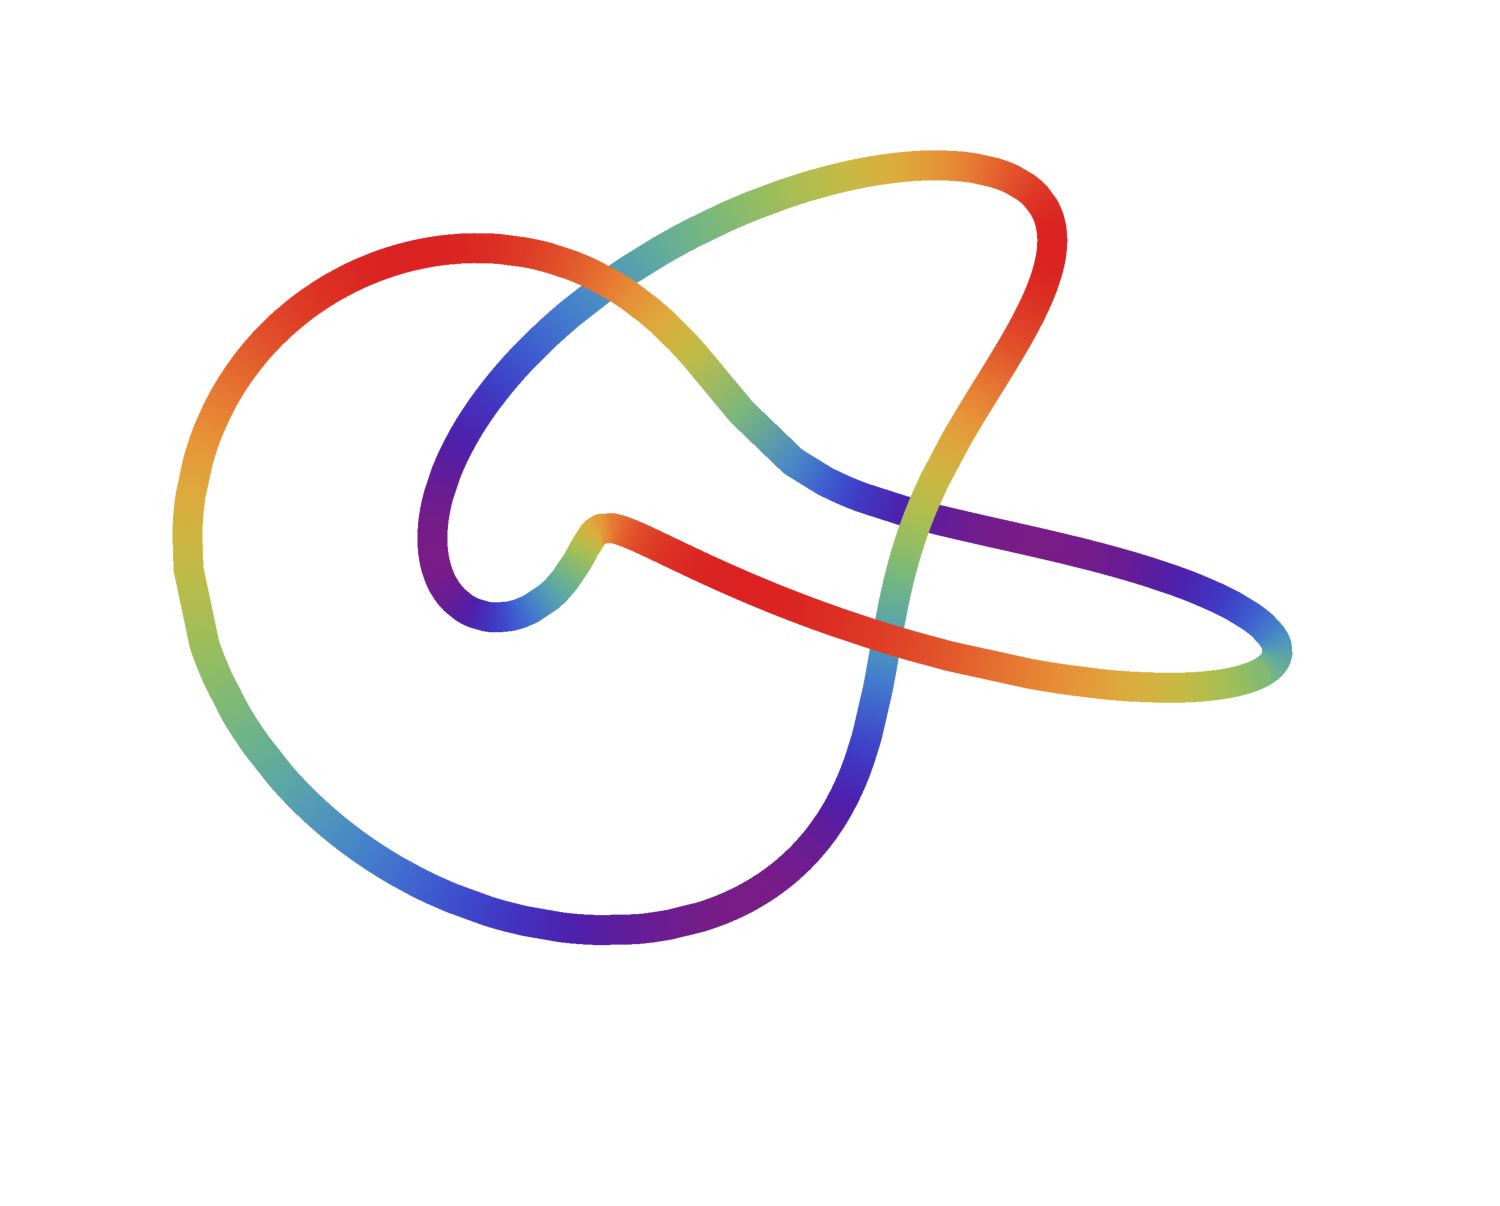
\includegraphics[width=\linewidth]{../data/torus-p2-q3.pdf}
        \subcaption{trójlistnik: $p = 2, q = 3$}
    \end{minipage}
    \begin{minipage}[b]{.3\linewidth}
        \centering
        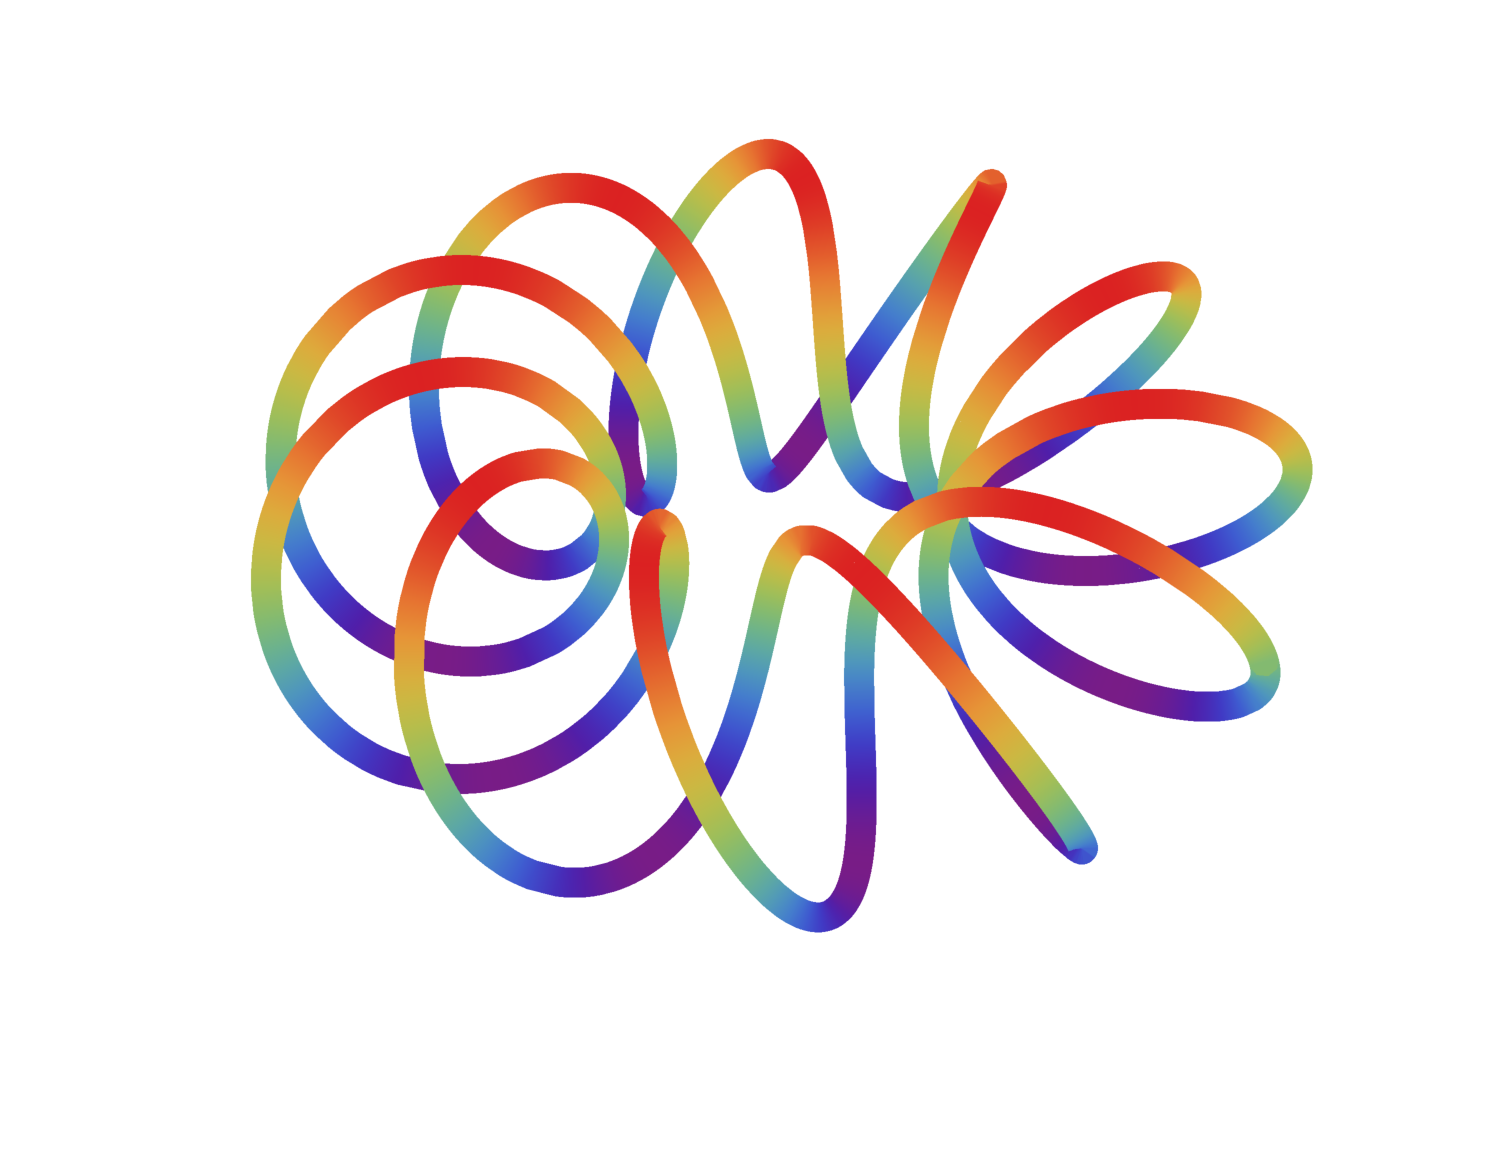
\includegraphics[width=\linewidth]{../data/torus-p2-q11.pdf}
        \subcaption{$p = 2, q = 11$}
    \end{minipage}
    \begin{minipage}[b]{.3\linewidth}
        \centering
        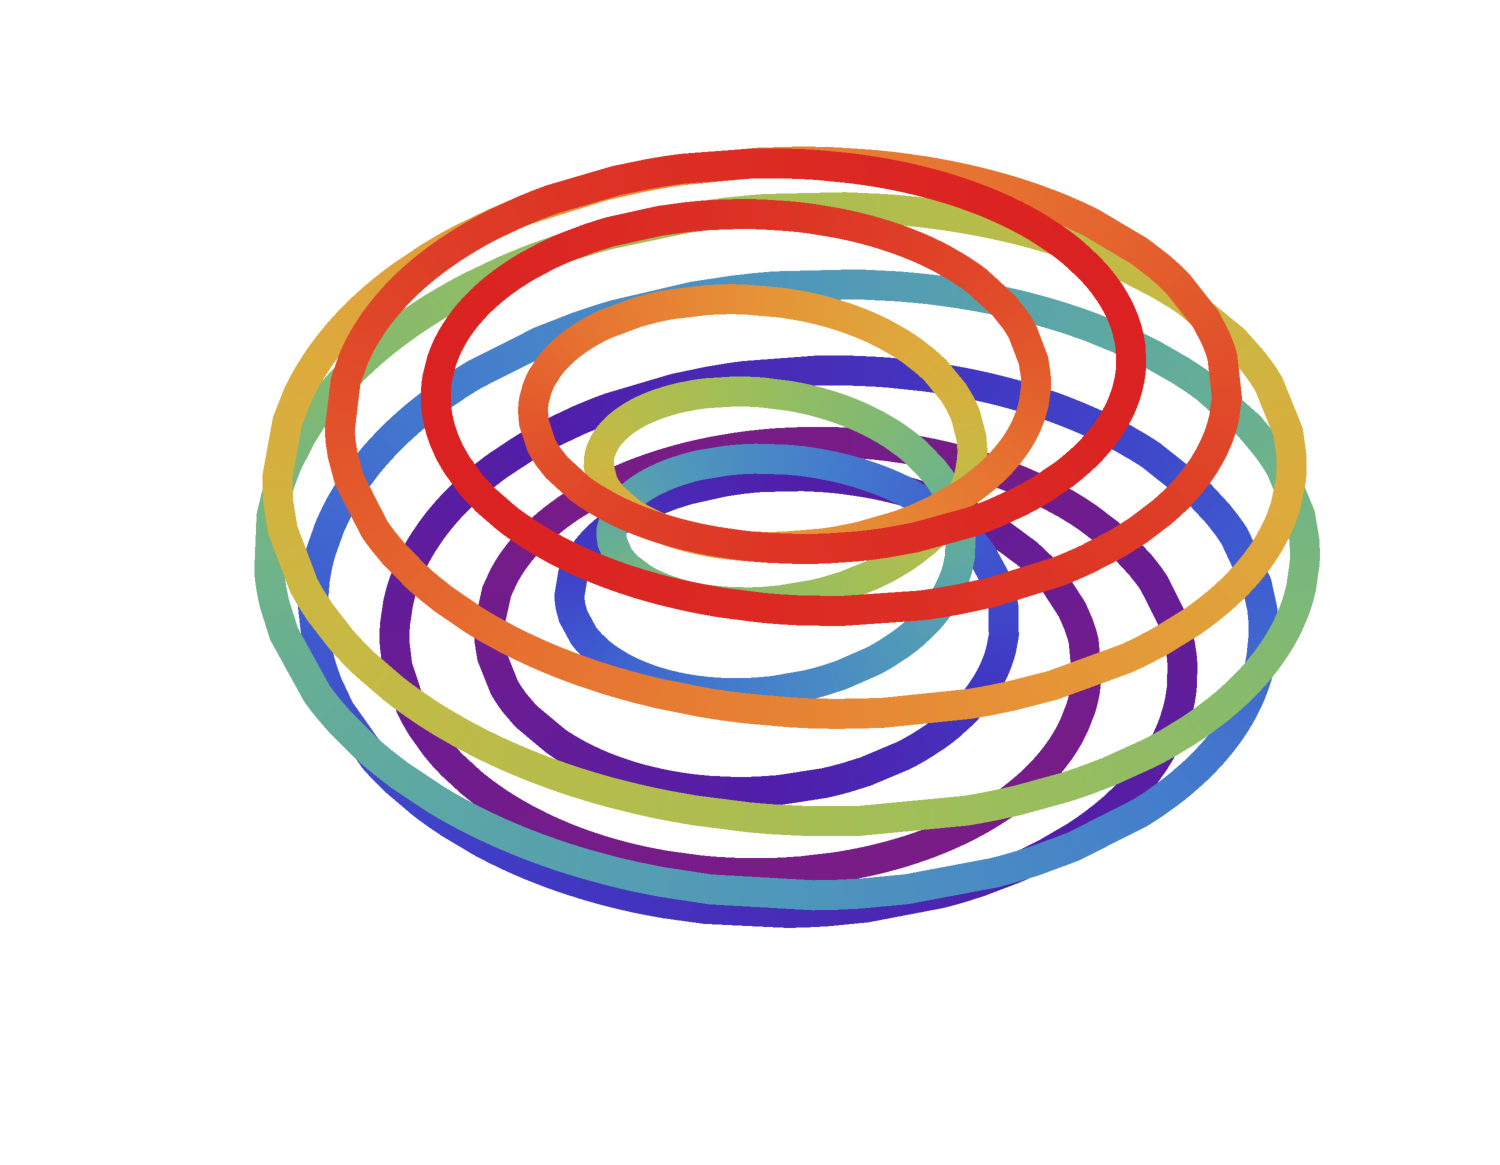
\includegraphics[width=\linewidth]{../data/torus-p11-q2.pdf}
        \subcaption{$p = 11, q = 2$}
    \end{minipage}
\end{figure}

%Węzeł ten leży na torusie $(r - 2)^2 + z^2 = 1$.
% p = 5;
% q = 3;
% ParametricPlot3D[
% {
% Cos [2 Pi p t] (2 + Cos[2 Pi q t]),
% (2 + Cos[2 Pi q t]) Sin[2 Pi p t],
% -Sin[2 Pi q t]},
% {t, 0, 1},
% ColorFunction -> "Rainbow",
% PlotStyle -> Thickness[0.02],
% Boxed -> False,
% Axes -> False
% ]

Okazuje się, że innych obiektów już nie ma.

\begin{proposition}
    Niech $K$ będzie splotem torusowym takim, że żadne z jego ogniw nie jest niewęzłem, czyli postaci $T_{1, 0}$.
    Wtedy dla pewnych całkowitch $p, q$, węzły $K$ oraz $T_{p, q}$ są tego samego typu.
\end{proposition}

\begin{proposition}
    Niech $d$ będzie największym wspólnym dzielnikiem liczb całkowitych $p, q$.
    Wtedy węzeł torusowy $T_{p, q}$ posiada dokładnie $d$ ogniw.
\end{proposition}

Siedem węzłów z tabeli na końcu książki to węzły torusowe.
Są to niewęzeł, $3_1 = T_{3,2}$, $5_1 = T_{5,2}$, $7_1 = T_{7,2}$, $8_{19} = T_{4,3}$, $9_1 = T_{9,2}$ oraz $10_{124} = T_{5, 3}$.

\begin{proposition}
    Niech $p, q$ będą względnie pierwszymi liczbami takimi, że $|p|, |q| \ge 2$.
    Wtedy splot $T_{p, q}$ oraz splot do niego odwrotny, $T_{-p, -q}$, są tego samego typu.
\end{proposition}

Sploty $T_{p, q}$ oraz $T_{q, p}$ również są równoważne.
Murasugi prezentuje w~swojej książce \cite{murasugi96} przyjemny dowód opierający się na następującym lemacie:

\begin{lemma}
    Sfera $S^3$ powstaje z~powierzchni dwóch węzłów trywialnych z~wnętrzem ($D^2 \times S^1$) przez wzajemne sklejenie południka i~równoleżnika z~równoleżnikiem i~południkiem.
\end{lemma}

\begin{proposition}
    Niech $K$ będzie nietrywialnym węzłem, którego grupa podstawowa $\pi$ ma nietrywialne centrum.
    Wtedy $K$ jest węzłem torusowym.
    % Kawauchi: The torus knots are characterized as the only knots whose groups have non-trivial centers (cf. Corollary 6.3.6).
\end{proposition}

\begin{proof}
\index[persons]{Aumann, Robert}
% https://mathscinet.ams.org/mathscinet-getitem?mr=96236
\index[persons]{Burde, Gerhard}%
\index[persons]{Murasugi, Kunio}%
\index[persons]{Neuwirth, Lee}%
\index[persons]{Nielsen, Jakob}%
\index[persons]{Stallings, John}%
\index[persons]{Zieschang, Heiner}%
    Najpierw pokazali to Murasugi \cite{murasugi61}, Neuwirth \cite{neuwirth61} przy dodatkowym założeniu, że węzeł $K$ jest alternujący,
    wkrótce po tym Burde, Zieschang znaleźli dowód w ogólnym przypadku \cite{zieschang66}.
    Ich dowód korzysta z wyników Neuwirtha (komutant grupy $\pi$ jest skończenie generowany), Stallingsa (dopełnienie $X$ tubularnego otoczenia $K$ można rozwłóknić nad $S^1$ z~włóknem: 2-rozmaitością $M$, z jedną krzywą na brzegu) i Nielsena.

    % TODO:
    (Burde, Zieschang piszą, że dla alternujących zrobił to już Aumann w 1956 roku).
\end{proof}

Węzły torusowe są pierwsze, czego dowód można znaleźć u Burdego, Zieschanga \cite[s. 95]{burde14}, chociaż nie wiem, kto pierwszy to zauważył.

Przejdźmy do podania wartości różnych niezmienników.


\subsection{Niezmienniki liczbowe węzłów torusowych}
Podamy teraz wartości całkowitoliczbowych niezmienników dla węzłów torusowych przy założeniu, że $p$ lub $q$ nie jest zerem.
Nietrywialne węzły torusowe są odwracalne, ale mają niezerową sygnaturę, więc nie są achiralne (chyba wiedział o tym Schreier \cite{schreier1924}).

\begin{proposition}
\index{okres}%
    Okresy splotu torusowego $T_{p, q}$ to dokładnie dzielniki $p$ lub $q$.
\end{proposition}

\begin{proof}
    Kawauchi \cite[ćw 10.1.9]{kawauchi1996}
\end{proof}

\begin{proposition}
\index{sygnatura}%
    Niech $p, q > 0$ będą liczbami całkowitymi, zaś $R_2$ oznacza resztę z dzielenia przez dwa.
    Zdefiniujmy funkcję $\sigma(p, q) = - \sigma(T_{p, q})$.
    % TODO: czemu ten minus? oni inaczej skierowane łuki mają?
    Spełnia zależność rekurencyjną
    \begin{equation}
        \sigma(p, q) = \begin{cases}
             q^2 + \sigma(p, p - 2q) - R_2(p)       & \text{jeśli } 2q < p, \\
             q^2 - 1                              & \text{jeśli } 2q = p, \\
             q^2 - \sigma(2q - p, q) + R_2(q) - 2 & \text{jeśli } 2q > p > q, \\
             \frac 12 (q^2 + R_2(q)) - 1                 & \text{jeśli } p = q,
             % czwarte stanowi algebraiczne przekształcenie trzeciego dla p >= q
        \end{cases}
    \end{equation}
    z warunkami brzegowymi: $\sigma(1, q) = 0$, $\sigma(2, q) = q-1$ oraz równość $\sigma(p, q) = \sigma(q, p)$.
\end{proposition}

\begin{proof}[Niedowód]
\index[persons]{Gordon, Cameron}%
\index[persons]{Litherland, Richard}%
\index[persons]{Murasugi, Kunio}%
\index[persons]{Brieskorn, Egbert}%
\index[persons]{Hirzebruch, Friedrich}%
    Gordon, Litherland, Murasugi \cite[tw. 5.2]{litherland1981} wspominają, że Brieskorn \cite{brieskorn1966} policzył sygnatury pewnych rozmaitości algebraicznych, co wystarcza do znalezienia sygnatury węzłów torusowych.
    Prowadzi to do takiego samego wzoru jak ten znaleziony przez Hirzebrucha \cite{hirzebruch1968}.
    Ale to wszystko jest trochę nieporęczne, dlatego używają niezmiennika acyklicznego (o~trywialnych zredukowanych grupach homologii; z~angielskiego \emph{null-homologous}) splotu $L$ w~zorientowanej 3-rozmaitości $M$ w~połączeniu z~jego $m$-krotnym rozgałęzionym nakryciem cyklicznym.
\index{wzór!Hirzebrucha}%
\end{proof}

Borodzik niedawno przyjrzał się dokładniej sygnaturom węzłów torusowych.
\index[persons]{Borodzik, Maciej}%
Razem z~Oleszkiewiczem \cite{borodzik2010} pokazał, że nie istnieje wymierna funkcja $R(p, q)$, która pokrywałaby się z sygnaturą węzła torusowego $T_{p, q}$ dla wszystkich względnie pierwszych, nieparzystych wartości $p$ oraz $q$.
\index[persons]{Oleszkiewicz, Krzysztof}%

\begin{proposition}
    Niech $p, q$ będą względnie pierwszymi liczbami, zaś $C \in [0, 1)$ stałą taką, że $Cpq$ nie jest liczbą całkowitą.
    Przyjmijmy $z = \exp (2 \pi i C)$ i zdefinujmy pomocnicze funkcje: niech $\{x\} = x - \lfloor x \rfloor$ oznacza część ułamkową, zaś
    \begin{equation}
        \langle x \rangle = \begin{cases}
            0 & \text{dla } x \in \Z \\
            \{x\} - 1/2 & \text{dla } x \not \in \Z
        \end{cases}
    \end{equation}
    funkcję piłę.
    Dalej, określmy sumę Dedekinda
    \begin{equation}
        s(p, q, x) = \sum_{j = 0}^{q-1} \left\langle \frac {j}{q} \right\rangle \left\langle \frac {jp}{q} + x \right\rangle.
    \end{equation}
    (Uwaga! Definicja funkcji $s$ z \cite{borodzik2010} zawiera złośliwą literówkę.)
    Przy tych oznaczeniach, sygnatura węzła $(p, q)$-torusowego wyznacza się wzorem
    \begin{align}
        \sigma(z) & = \frac{1}{3pq} \left(p^2 + q^2 + 6 \langle Cpq \rangle^2 - \frac {1}{2} \right)  + 2(C^2 - C) pq + (2-4C) \langle Cpq \rangle + {} \\
        & - 2s(p, q, Cp) - 2s(q, p, Cq) - 2s(p, q, p-pC) - 2s(q, p, q-qC). \nonumber
    \end{align}
\end{proposition}

\begin{corollary}
    Jeśli $p, q$ są nieparzyste i względnie pierwsze, to
    \begin{equation}
        \sigma(T_{p,q}) = \frac{1}{6pq} + \frac{2p}{3q} + \frac{2q}{3p} - \frac{pq}{2} - 4(s(2p, q, 0) + s(2q, p, 0)) - 1.
    \end{equation}
\end{corollary}

\begin{corollary}
    Jeśli $p$ jest nieparzyste, zaś $q > 2$ parzyste, to
    \begin{equation}
        \sigma(T_{p,q}) = - \frac{pq}{2} + 4s(2p, q, 0) - 8s(p, q, 0) + 1.
    \end{equation}
\end{corollary}

Wyznaczenie liczby gordyjskiej było dużo trudniejsze.
Murasugi \cite[s. 150]{murasugi1996} proponuje Czytelnikowi pokazanie, że zachodzi równość $\unknotting T_{p, 2} = \frac 12 (|p| - 1)$ oraz nierówność
\begin{equation}
    u(T_{p, q}) \le \frac 12 (p-1)(q-1).
\end{equation}

Milnor \cite[uwaga 10.9]{milnor1968} postawił hipotezę, że znak $\le$ można zamienić na $=$.
\index{hipoteza!Milnora}%
Pierwszy dowód znaleźli Kronheimer, Mrówka \cite{kronheimer1993}, \cite{kronheimer1995}: panowie pokazali, że jeśli $X$ jest gładką, jednospójną, domkniętą i zorientowaną 4-rozmaitością; posiada nietrywialny wielomianowy niezmiennik Donaldsona oraz wymiar maksymalnej dodatniej podprzestrzeni dla formy przecięć drugiej homologii jest nieparzysty, większy od 2, to genus każdej zorientowanej, gładko zanurzonej powierzchni $F$ (poza dwoma wyjątkami, których nie rozumiemy), spełnia nierówność $2g - 2 \ge F \cdot F$.
Ugh!

Później Rasmussen \cite{rasmussen2010} podał inny dowód, który nie wykorzystuje już cechowania (\emph{gauge theory}), tylko homologię Chowanowa.
% 04 - ArXiV, 10 - peer reviewed
\index[people]{Rasmussen, Jacob}%

\begin{proposition}
\index{liczba gordyjska}%
\label{prp:torus_unknotting_number}%
    Dla względnie pierwszych $p, q > 0$ mamy
    \begin{equation}
        \unknotting T_{p, q} = \frac 12 (p - 1)(q - 1),
    \end{equation}
\end{proposition}

\begin{proposition}
    \index{genus}%
    Dla względnie pierwszych $p, q > 0$ mamy
    \begin{equation}
        \genus T_{p, q} = \frac 12 (p - 1)(q - 1),
    \end{equation}
\end{proposition}

\begin{proof}
    Wyznacznik macierzy Seiferta węzła torusowego jest niezerowy, więc genus równa się stopniu wielomianu Alexandera.
    Patrz też \cite[s. 149]{murasugi1996}.
\end{proof}

\begin{proposition}
\index{liczba mostowa}%
    $\bridge T_{p, q} = \min \{|p|, |q|\}$
\end{proposition}

Według Murasugiego \cite[s. 150]{murasugi1996} dowód znalazł Schubert \cite{schubert1954}.
\index[persons]{Schubert, Horst}%

\begin{corollary}
\index{indeks!warkoczowy}%
\label{cor:torus_braid_number}%
    Niech $p, q \neq 0$ będą liczbami całkowitymi.
    Wtedy $\braid T_{p, q} = \min \{|p|, |q|\}$.
\end{corollary}

\begin{proof}
    Niech $K$ będzie węzłem torusowym typu $(p,q)$ z~minimalnym przedstawieniem jako warkocz $\beta$.
    Z konstrukcji domknięcia (czyli dołączenia rozłącznych półokręgów) wynika,
    że diagram $K$ ma dokładnie $b(K)$ lokalnych maksimów.
    Definicja liczby mostowej orzeka, iż $\bridge K \le \braid K$.
    Bez straty ogólności niech $p > q > 0$.
    Skoro węzeł $K$ powstaje z~$q$-warkocza $(\sigma_{q-1} \ldots \sigma_2\sigma_1)^p$,
    indeks $b(K)$ nie przekracza $q = br(K)$.
\end{proof}

\begin{proposition}
\index{indeks!skrzyżowaniowy}%
    Mamy $\crossing T_{p, q} = |pq| - \max\{|p|, |q|\}$.
\end{proposition}
    
\begin{proof}
\index[persons]{Murasugi, Kunio}%
    Murasugi \cite[s. 255]{murasugi1991} zauważył, że jeśli $\gamma$ jest jednorodnym $n$-warkoczem, gdzie $n = \braid(\widehat{\gamma})$, zaś $d_i$ to suma wykładników przy $\sigma_i$ w $\gamma$, to $\crossing \widehat{\gamma} = \sum_{i=1}^{n-1} |d_i|$.
    Ale splot torusowy $T_{p, q}$, gdzie $2 \le p \le q$, można przedstawić jako domknięcie jednorodnego $p$-warkocza $(\sigma_1 \sigma_2 \cdot \ldots \cdot \sigma_{p-1})^q$, co kończy natychmiast dowód.
\end{proof}



\subsection{Niezmienniki wielomianowe węzłów torusowych}
\begin{proposition}
    Niech $L = T_{p, q}$ będzie splotem torusowym o $d$ ogniwach, różnym od $T_{0, 0}$.
\index{wielomian!Alexandera}%
    Wtedy jego wielomianem Alexandera jest
    \begin{equation}
        \alexander_L(t) = (-1)^{d-1} \frac{(1-t)(1 - t^{pq/d})^d}{(1-t^p)(1-t^q)} \cdot t^{-(p-1)(q-1)/2}.
    \end{equation}
\end{proposition}

Przypadek $p = 2$ wymaga prostego rozumowania indukcyjnego.
Samo ćwiczenie pojawia się w~wielu podręcznikach topologii.
Pełny dowód można znaleźć w~\cite[przykład 9.15]{burde14}, gdzie wyznaczono jakobian prezentacji grupy węzła $\langle x, y \mid x^py^{-q}\rangle$.

Inne podejście, formułę Seiferta-Torresa, prezentuje przeglądowa praca Turaewa \cite{turaev86}.
\index{formuła Seiferta-Torresa}

\begin{proof}
    Macierz Seiferta węzła torusowego $L = T_{p, q}$ ma nieskomplikowaną blokową budowę i posłuży nam do znalezienia wielomianu Alexandera wzorem $\alexander = \det (M - tM^t)$.
    % Rachunki są nieco uciążliwe.
    \begin{equation}
        M = \begin{bmatrix}
            B & & & & \\
            -B & B & & & \\
            & \ddots & \ddots & & \\
            & & \ddots & B & \\
            & & & -B & B
        \end{bmatrix},
    \end{equation}
    złożona z~$(q-1)^2$ bloków o~wymiarach $(p-1) \times (p-1)$:
    \begin{equation}
        B = \begin{bmatrix}
            -1 & & & & \\
            1 & -1 & & & \\
            & 1 & \ddots & & \\
            & & \ddots & -1 & \\
            & & & 1 & -1
        \end{bmatrix}.
    \end{equation}
    Rachunki pozostawiamy Czytelnikowi jako ćwiczenie.
\end{proof}

\begin{corollary}
    Niech $K = T_{p, q}$ będzie węzłem torusowym.
    Wtedy jego wielomianem Alexandera jest
    \begin{equation}
         \alexander(t) = \frac{(t^{pq}-1)(t-1)}{(t^p-1)(t^q-1)}.
    \end{equation}
\end{corollary}

\begin{corollary}
    Wielomian Alexandera odróżnia od siebie węzły $(2,n)$-torusowe.
\end{corollary}

\begin{proof}
    Mamy $\alexander(T_{2,n})(t) = (t^n+1) / (t+1)$, więc $\deg \alexander (T_{2,n}) = n - 1$.
\end{proof}

Znajomość wielomianu Alexandera wystarcza na szczęście do podania pełnej klasyfikacji węzłów torusowych bez uciążliwego dowodu.

\begin{proposition}
    Niech $p, q, r, s$ będą liczbami całkowitymi.
    Następujące warunki są równoważne:
    \begin{itemize}
        \item węzły torusowe $T_{q, r}$ oraz $T_{p, s}$ są równoważne,
        \item $\{q, r\} = \{p, s\}$ lub $\{q, r\} = \{-p, -s\}$.
    \end{itemize}
\end{proposition}

\begin{proof}
    Ograniczymy się do przypadku, gdy $p, q, r, s \ge 2$.
    Tylko jedna implikacja wymaga dowodu, w~prawo.
    Bez straty ogólności załóżmy więc, że $q > r$, $p > s$.
    Skoro węzły $T_{q, r}$ i~$T_{p,s}$ są równoważne, to porównanie najwyższych współczynników w~ich wielomianach Alexandera daje równość $(q-1)(r-1) = (p-1)(s-1)$.
    Wymnożenie wszystkiego prowadzi do czterech przypadków: $s = r$, $s = ps$, $qr = r$, $qr = ps$, z~których dwa środkowe nie mogą zachodzić (gdyż $p, q > 1$).
    Z czwartego wynika, że $qr \le s < ps$, czyli sprzeczność.
\end{proof}

Kawauchi pisze, że wcześniej klasyfikacja węzłów torusowych wynikała z klasyfikacji wolnych produktów $(\Z/p) * (\Z/q)$, które są ilorazami grup węzłów torusowych \cite{schreier24}.

Wartości wielomianu Jonesa podajemy bez dowodu:

\begin{proposition}
\index{klamra Kauffmana}%
    Klamra Kauffmana spełnia zależność rekurencyjną
    \begin{equation}
        \bracket{T_{2, n}} = A \bracket{T_{2,n-1}} + (-1)^{n-1} A^{2-3n}
    \end{equation}
    z warunkiem brzegowym $\bracket{T_{2,1}} = -A^3$.
\end{proposition}

\begin{proposition}
\index{wielomian!Jonesa}%
    Niech $L = T_{p, q}$ będzie węzłem torusowym.
    Wtedy jego wielomianem Jonesa jest
    \begin{equation}
        \jones(t) = \frac {{\sqrt t}^{(p-1)(q-1)}}{1-t^2} \cdot (1 - t^{p+1} - t^{q+1} + t^{p+q}).
    \end{equation}
\end{proposition}

\index{węzeł!torusowy|)}%

% Koniec sekcji Węzły torusowe



\section{Węzły satelitarne} % (fold)

% meridian - południk
% longitude - równoleżnik
Załóżmy, że w dopełnieniu pewnego splotu został zanurzony torus.
Jeżeli jest ściśliwy, to albo równoleżnikl torusa ogranicza dysk w dopełnieniu splotu~i torus jest niezawęźlony, albo południk ogranicza dysk w dopełnieniu splotu i~splot nie przebiega wzdłuż torusa.
Żadna z~tych sytuacji nie jest ciekawa.
Inny zdegenerowany przypadek występuje, gdy torus stanowi rurowe otoczenie jednego z~ogniw splotu.
W przeciwnym razie splot można zbudować z~prostszych obiektów.

Oto formalny opis konstrukcji.
Niech $W$ będzie pełnym torusem.
Dysk zanurzony w $W$, którego brzeg stanowi nieściągalną pętlę w $\partial W$, nazywamy południkowym.
Mówimy, że zamknięta krzywa $\lambda \subseteq W$ jest właściwa, jeżeli przecina wszystkie dyski południkowe.

\begin{definition}[węzeł satelitarny]
    \index{węzeł!satelitarny}
    Niech $P$ będzie splotem zanurzonym w~niezawęźlonym torusie $W$ tak, by co najmniej jedno z~ogniw stanowiło właściwą pętlę w~$W$.
    Niech $C$ będzie węzłem, zaś $V$ jego rurowym otoczeniem.
    Wybierzmy dowolny homeomorfizm $h \colon W \to V$.
    Wtedy splot $S = h(P)$ nazywamy satelitą o~wzorcu $P$ oraz towarzyszu $C$.
\end{definition}

% \begin{definition}
%     Węzeł nazywamy satelitarnym, jeśli zawiera nieściśliwy, nierównoległy do brzegu torus we własnym dopełnieniu.
% \end{definition}

Hoste i inni podejrzewają w~\cite{thistlethwaite98}, że jeśli satelita owija się $m$-krotnie wokół torusa, zaś indeks skrzyżowaniowy towarzysza wynosi $k$, to satelita nie posiada diagramu o~mniej niż $km^2$ skrzyżowaniach.
\index[persons]{Hoste, Jim}%
\index[persons]{Thistlethwaite, Morwen}%
\index[persons]{Weeks, Jeff}%

Ponieważ dla trójlistnika $k = 3$, napotkali się tylko na satelity owijające się $m = 2$ razy podczas tablicowania pierwszych węzłów do 16 skrzyżowań.
Nie spodziewano się żadnego satelity ósemki, gdyż wtedy $k = 4$, zatem każdy satelita miałby co najmniej $4 \cdot 2^2 + 1 = 17$ skrzyżowań: dodatkowe $+1$ jest potrzebne, by nie dostać splotu o~dwóch ogniwach.

Najprostszy satelita ma 13 skrzyżowań.

\begin{example}[swallow-follow torus]
    Klasa węzłów satelitarnych obejmuje węzły złożone.
    W ich przypadku można wskazać pewien szczególny torus nieściśliwy -- połykający pierwszy składnik, a~potem podążający za drugim:\footnote{Źródło: \url{https://mcm-www.jwu.ac.jp/~hayashic/semi/07/07i/07i.html}}
    \begin{figure}[H]
        \centering
        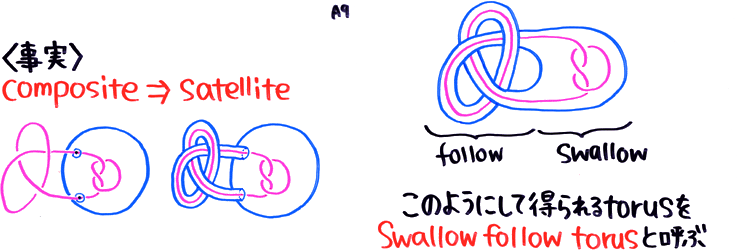
\includegraphics[width=0.75\linewidth]{../data/mixed/follow-swallow.png}
        \caption[something]{Torus połykająco-podążający. Źródło: strona internetowa\footnote{\url{https://mcm-www.jwu.ac.jp/~hayashic/semi/07/07i/07i.html}.} C. Hayashiego.}
    \end{figure}
\end{example}

Schubert pokazał, że zorientowane klasy izotopii węzłów w~$S^3$ tworzą wolny przemienny monoid na przeliczalnie wielu generatorach.
\index[persons]{Schubert, Horst}%
Dowód to uważna analiza nieściśliwych torusów obecnych w~dopełnieniu sumy spójnej.
To doprowadziło go do definicji węzłów satelitarnych i~towarzyszących w~przełomowej pracy \cite{schubert53} oraz zunifikowało teorię 3-rozmaitości z teorią węzłów.
Patrz też \cite{motegi97} (Wikipedia mówi, że zapis węzła jako satelity nie jest jednoznaczny, a~tu mogą być przykłady.)
%=% https://en.wikipedia.org/wiki/Satellite_knot#cite_ref-7

Na brzegu torusa $V$ można wprowadzić pewien układ współrzędnych: południk to pętla właściwa w $\partial V$, która ogranicza dysk w $V$, natomiast równoleżnik to pętla w $\partial V$, która spotyka południk raz.
Z~dokładnością do izotopii południk jest jeden, ale równoleżnik nie.
Gdy indeks zaczepienia równoleżnika oraz rdzenia torusa wynosi zero, mówimy, że równoleżnik jest preferowany.

\begin{definition}[dubel Whiteheada]
    \index{dubel Whiteheada}
    Jeżeli $P \subseteq W$ jest skręconym jednokrotnie niewęzłem, to węzeł $S$ nazywamy dublem Whiteheada.
\end{definition}

Każdy węzeł posiada nieskończenie wiele dubli Whiteheada: wystarczy rozciąć torus $V$, skręcić jedną końcówkę i~ponownie zszyć, żaden z~nich nie jest odróżniany od niewęzła przez wielomian Alexandera.

Wyróżnia się pewien szczególny homeomorfizm $h$, który przenosi południk i preferowany równoleżnik $W$ na południk i preferowany równoleżnik $V$.
Nazywamy go wiernym.
% faithful
O dublu względem wiernego homeomorfizmu mówimy, że jest nieskręcony.

\begin{definition}[węzeł kablowy]
    \index{węzeł!kablowy}
    Niech $h \colon W \to V$ będzie wiernym homeomorfizmem, zaś $P$ węzłem $(p, q)$-torusowym.
    Satelitę $S$ nazywamy węzłem $(p, q)$-kablowym albo krótko kablem.
\end{definition}

\begin{proposition}
    Każdy kabel wyznacza jednoznacznie węzeł, z~którego powstał.
\end{proposition}

\begin{proof}
\index[persons]{Feustel, Charles}%
\index[persons]{Whitten, Wilbur}%
    Wniosek 2 z~pracy \cite{feustel78} Feustela, Whittena pokazuje, że na podstawie kabla można wyznaczyć parametry węzła torusowego $K'_{p,q}$ oraz topologię dopełnienia oryginalnego węzła.
    Wiemy jednak z~twierdzenia Gordona-Lueckego, że różne węzły PIERWSZE mają różne dopełnienia.
\end{proof}

Niewęzeł nie ma nietrywialnych węzłów towarzyszących.

\begin{definition}
    Towarzysza $C$ nietrywialnego splotu nazywamy właściwym, jeśli nie jest niewęzłem i~nie jest ogniwem tego splotu.
\end{definition}

Sploty bez właściwych towarzyszy określa się zazwyczaj terminem ,,atoroidalny''.
Patrz też diagram przedstawiony w \cite{cromwell04} na stronie 83.

\begin{proposition}
    Duble nietrywialnych węzłów oraz kable są pierwsze.
\end{proposition}

\begin{proof}
    Prosty wniosek z~twierdzenia 4.4.1 w~\cite[s. 84]{cromwell04}: jeżeli wzorzec jest niewęzłem lub węzłem pierwszym, to każdy właściwy satelita jest pierwszy.
\end{proof}

Niektóre węzły przedstawiają się jako satelity w~dokładnie jeden sposób, inne nie.
Rok 1979 przyniósł amerykańską pracę \cite{jaco79} oraz niemiecką książkę\footnote{Według recenzji Hempela, najważniejsze tam jest twierdzenie klasyfikacyjne: niech $M_1, M_2$ będą 3-rozmaitościami Hakena z brzegiem, zaś $V_1, V_2$ ich podrozmaitościami charakterystycznymi, wtedy każda homotopijna równoważność $f \colon M_1 \to M_2$ można zdeformować tak, że jest homeomorfizmem między domknięciami: $M_1 \setminus V_1$ oraz $M_2 \setminus V_2$ i~homotopijną równoważnością między $V_1$ oraz $V_2$.} \cite{johannson79}, gdzie niezależnie od siebie opisano jednoznaczny rozkład, nazywany teraz rozkładem Jaco-Shalena-Johannsona:
\index[persons]{Jaco, William}%
\index[persons]{Shalen, Peter}%
\index[persons]{Johannson, Klaus}%

\begin{proposition}
    Niech $M$ będzie nierozkładalną, orientowalną, domkniętą 3-rozmaitością.
    Istnieje wtedy jedyna z dokładnością do izotopii minimalna rodzina rozłącznie zanurzonych nieściśliwych torusów tak, że każda składowa 3-rozmaitości powstałej przez rozcinanie wzdluż torusów jest atoroidalna lub włóknistą przestrzenią Seiferta ($S^1$-wiązką nad dwuwymiarowym orbifoldem).
\end{proposition}

Jest on związany z operacją splatania (ang. \emph{splicing}), będącej uogólnieniem budowania satelitów.
Hipotezę o jedyności rozkładu wysnuł wcześniej Waldhausen.
\index[persons]{Waldhausen, Friedhelm}%

% Koniec sekcji Węzły satelitarne


\section{Węzły hiperboliczne}
\index{węzeł!hiperboliczny|(}
\label{sec:hyperbolic}
Jak pisaliśmy w~sekcji \ref{sec:mutant}, słynne węzły Conwaya oraz Kinoshity-Terasakiego odróżnił od siebie po raz pierwszy Riley.
\index{węzeł!Conwaya}%
\index{węzeł!Kinoshity-Terasakiego}%
Zbadał paraboliczne reprezentacje ich grup w~skończoną grupę prostą $PSL(2, 7)$, co doprowadziło go do odkrycia struktury hiperbolicznej w~dopełnieniu ósemki \cite{riley75}.
\index{ósemka}
% https://arxiv.org/pdf/2002.00564.pdf
Zainspirowany tym wynikiem Thurston najpierw rozłożył dopełnienie ósemki na dwa idealne wielościany, a~potem znacznie uogólnił swój przykład.

Reszta sekcji powstała na podstawie dwóch źródeł: przeglądowej pracy Kalfagianniego, Futera oraz Purcell \cite{purcell19} i~notatek z~wykładów, które były prowadzone przez samą Purcell.
Wiedzę o~węzłach hiperbolicznych można czerpać także z~artykułu Weeksa \cite{weeks05}.

% Badając sploty nie ograniczamy się tylko do diagramów, ale korzystamy też z ich dopełnień, to znaczy 3-rozmaitości $S^3 \setminus L$.
% Jest ona homeomorficzna z wnętrzem zwartej rozmaitości $X(L) = S^3 \setminus N(K)$, zwanej zewnętrzem splotu, gdzie $N(L)$ stanowi rurowe otoczenie splotu.
% Dalej możemy stosować maszynierę topologii 3-rozmaitości.

% \begin{definition}[ściśliwy]
%     Niech orientowalna powierzchnia $S$ będzie właściwie\footnote{properly} zanurzona w zwartej, orientowalnej 3-rozmaitości $M$.
%     Załóżmy, że dla każdego dysku $E \subseteq M$ z brzegiem $\partial E \subseteq S$ istnieje dysk $E' \subseteq S$ taki, że $\partial E = \partial E'$.
%     Mówimy wtedy, że powierzchnia $S$ jest nieściśliwa.
% \end{definition}

% $\partial$-ściśliwość

% essential

% Haken

% monodromy of fibration

% Węzły i sploty, które będziemy rozpatrywać dalej, mają szczególną strukturą geometryczną.

\begin{definition}[hiperboliczny]
    Splot $L$, na dopełnieniu którego można zadać zupełną metrykę o~stałej krzywiźnie $-1$ nazywamy hiperbolicznym.
\end{definition}

\begin{proposition}
    Niech $L$ będzie splotem, zaś $\mathbb H^3$ hiperboliczną 3-przestrzenią.
    Splot $L$ jest hiperboliczny wtedy i~tylko wtedy, gdy $S^3 \setminus L = \mathbb H^3 / \Gamma$, gdzie $\Gamma$ jest dyskretną, beztorsyjną grupą izometrii, izomorficzną z~$\pi_1(S^3 \setminus L)$.
\end{proposition}
% TODO: skąd to jest dokładnie?

Thurston podejrzewał, że każda 3-rozmaitość rozkłada się wzdłuż sfer i~nieściśliwych torusów na części wyposażone w~jedną z~ośmiu kanonicznych geometrii:
\begin{itemize}
\item sferyczną $S^3$, albo euklidesową $E^3$, albo hiperboliczną $H^3$,
\item $S^2 \times \R$, albo $H^2 \times \R$,
\item uniwersalne nakrycie $SL(2, \R)$,
\item geometrię Sol albo geometrię Nil.
\end{itemize}
Nie umiał podać pełnego uzasadnienia, w~pracy \cite{thurston82} udowodnił swoje przypuszczenie dla rozmaitości Hakena.
\index{rozmaitość Hakena}
Dowód hipotezy geometryzacyjnej dostarczył mniej więcej dwie dekady później Perelman, nie to jest jednak dla nas najważniejsze.
\index{hipoteza!geometryzacyjna Thurstona}
Z przełomowych prac Thurstona z~lat 70. oraz 80. wynika coś ciekawszego: że dopełnienie węzła jest rozmaitością włóknistą Seiferta, toroidalną albo hiperboliczną.
Innymi słowy, Thurston przedstawił trychotomię:

\begin{theorem}
    \index{twierdzenie!Thurstona}
    Każdy węzeł jest satelitarny, torusowy albo hiperboliczny.
    \index{węzeł!satelitarny}
    \index{węzeł!torusowy}
\end{theorem}
% luźno związane: http://www.deltami.edu.pl/temat/matematyka/topologia/2012/12/27/%William_Thurston_i_hipoteza_geometryzacyjna/

\begin{proof}
    Thurston w~\cite{thurston82}.
\end{proof}

Węzły hiperboliczne stanowią najliczniejszą i~najmniej zrozumianą rodzinę węzłów.
Sam Nead, użytkownik portalu MathOverflow napisał, że kryterium Thurstona dzięki maszynerii JSJ oraz pracom innych osób można wysłowić algebraicznie.

\begin{proposition}
    % There is a topological criterion due to Thurston.  Using the JSJ machine (and work of many others) this criterion can also be phrased algebraically.  I'll essay these below.  Please note that the situation is much simpler for knots.  To answer your question most directly, here is the desired reference to Wikipedia.
    % http://en.wikipedia.org/wiki/Hyperbolic_link
    % This page refers to the books of Colin Adams and William Thurston.  Both are excellent.
    % Now, here is Thurston's criterion. (EDIT: exposition improved after reading Bruno Martelli's answer.)
    % Suppose that $L$ is the link and $X$ is the link complement.  Suppose $\pi = \pi_1(X)$. We assume the following properties (and each property assumes the proceeding ones). $\newcommand{\ZZ}{\mathbb{Z}}$
    %  - $L$ is not a split link.  Equivalently, $X$ is contains no essential two-sphere.  Equivalently, $\pi$ is not a free product.
    %  - $L$ is not the unknot. Equivalently, $X$ contains no essential disk. Equivalently, $\pi$ is not $\ZZ$.
    %  - $L$ has no component that is an "undisturbed satellite knot".  Equivalently, $X$ contains no essential torus.
    %  - $L$ is not a torus knot. Equivalently, $X$ contains no essential annulus. These last two topological properties are equivalent to $\pi$ not containing a copy of $\ZZ^2$.
    % Then $X$ admits a hyperbolic structure.
    Niech $L$ będzie splotem, który nie rozszczepia się, nie jest niewęzłem, nie posiada wśród ogniw niezakłóconego węzła satelitarnego oraz nie jest węzłem torusowym.
    \index{splot!rozszczepialny}
    Wtedy $L$ jest hiperboliczny.
\end{proposition}

\begin{proposition}
    Niech $L$ będzie splotem takim, że jego dopełnienie $S^3 \setminus L$ nie zawiera właściwej 2-sfery, właściwego dysku, właściwego torusa oraz właściwego pierścienia.
    Wtedy $L$ jest hiperboliczny.
\end{proposition}

\begin{proposition}
    Niech $L$ będzie splotem takim, że jego grupa $\pi(S^3 \setminus L)$ nie jest produktem wolnym, nie jest izomorficzna z~$\Z$ oraz nie zawiera w~sobie kopii grupy $\Z \oplus \Z$.
    Wtedy $L$ jest hiperboliczny.
\end{proposition}

\begin{proof}
    Patrz \url{https://mathoverflow.net/a/153327}.
\end{proof}

Czas na podanie jakichś przykładów węzłów hiperbolicznych, za \cite{adams05}.

\begin{proposition}
    Każdy alternujący, pierwszy, oraz nierozszczepialny splot jest albo 2-warkoczem (a zatem, torusowy) albo hiperboliczny.
    \index{węzeł!alternujący}
    \index{węzeł!pierwszy}
    \index{węzeł!rozszczepialny}
\end{proposition}

\begin{proof}
    Menasco \cite{menasco84} pokazał, że dopełnienie alternującego węzła nie zawiera nieściśliwych  nieperyferyjnych torusów.
    To w~połączeniu z~unifikacyjnym twierdzeniem Thurstona dla rozmaitości Hakena kończy dowód.
\index{rozmaitość Hakena}%
    % zarys dowodu zz MathSciNet
\end{proof}

\begin{proposition}
    Nietrywialne pierwsze prawie alternujące węzły są torusowe albo hiperboliczne.
    \index{węzeł!pierwszy}
    \index{węzeł!prawie alternujący}
\end{proposition}

\begin{proof}
    Grupa studentów pod opieką Adamsa w \cite{brock92}.
\end{proof}

\begin{proposition}
    Toroidalnie alternujące węzły pierwsze są torusowe albo hiperboliczne.
    \index{węzeł!pierwszy}
    \index{węzeł!toroidalnie alternujący}
\end{proposition}

Ze wszystkich węzłów pierwszych do 11 skrzyżowań i~pierwszych, nierozszczepialnych splotów do 10 skrzyżowań tylko 3 węzły i~2 sploty nie są toroidalnie alternujące, tak twierdzi Adams \cite{adams05}.

\begin{proof}
    Patrz \cite{adams994}.
\end{proof}

\begin{proposition}
    Sploty Montesinosa są prawie zawsze torusowe albo hiperboliczne.
    \index{splot!Montesinosa}
\end{proposition}

\begin{proof}
    Najpierw zidentyfikowano sploty Montesinosa torusowe, które są też torusowe \cite{boileau80}.
    Potem w~pracy \cite{oertel84} znaleziono listę wyjątków (z chyba trochę inną notacją niż nasza):
    \begin{itemize}
        \item $K(1/2, 1/2, 21/2, 21/2)$,
        \item $K(2/3, 21/3, 21/3)$,
        \item $K(1/2, 21/4, 21/4)$,
        \item $K(1/2, 21/3, 21/6)$,
        \item lub lustra tych splotów. \qedhere
    \end{itemize}
\end{proof}

\begin{proposition}
    Mutant węzła hiperbolicznego jest węzłem hiperbolicznym.
    \index{mutant}
\end{proposition}

\begin{proof}
    Ruberman w~\cite{ruberman87}, patrz wniosek 1.4.
\end{proof}

\begin{proposition}
    Niech $G$ oznacza grupę izometrii wnętrza dopełnienia węzła hiperbolicznego.
    Wtedy $G$ jest diedralna lub skończona cykliczna.
\end{proposition}

\begin{proof}
    Pierwszy był Riley w~artykule \cite[s. 124]{riley79}, można też zapoznać się z~późniejszą pracą \cite{kodama92} Kodamy i Sakumy.
    % Kodama - lemat_1.1
\end{proof}

Kawauchi \cite[s. 131]{kawauchi96} wprowadza jeszcze jedną grupę (grupę symetrii węzła): iloraz grupy PL automorfizmów pary $(S^3, K)$ przez podgrupę elementów, które są otaczająco izotopijne z~odwzorowaniem tożsamościowym.
Okazuje się, że nie wszystkie są skończone:

\begin{proposition}
    Węzeł $K$ ma skończoną grupę symetrii wtedy i~tylko wtedy, gdy jest hiperboliczny, torusowy lub kablem węzła torusowego.
\end{proposition}

Kawauchi nie podaje dowodu, ale zaleca zajrzeć do pracy Sakumy.
Ja zajrzałem i dalej nie mam pojęcia, jak ten dowód miałby wyglądać.

Z kryterium Thurstona mamy prosty wniosek (bo węzły złożone są satelitarne):

\begin{corollary}
    Każdy węzeł hiperboliczny jest pierwszy.
    \index{węzeł!pierwszy}
\end{corollary}

Prawie każdy węzeł pierwszy o~mniej niż 17 skrzyżowaniach jest hiperboliczny, na 32 wyjątki składa się 12 węzłów torusowych oraz 20 satelitów trójlistnika.
Te ostatnie mają co najmniej 13 skrzyżowań.
Baza ciągów liczb całkowitych OEIS zawiera informacje na temat liczności poszczególnych typów węzłów.
Analizując ciągi A051764, A051765 oraz A052408 można dojść do wniosku, że wraz ze wzrostem liczby skrzyżowań, stosunek liczby węzłów hiperbolicznych do wszystkich węzłów dąży do $1$:

\begin{figure}[H]
\renewcommand*{\arraystretch}{1.4}
\footnotesize
\begin{longtable}{lcccccccccccccc}
\hline
    \textbf{rodzaj} & 3 & 4 & 5 & 6 & 7 & 8  & 9  & 10  & 11  & 12   & 13   & 14    & 15     \\ \hline \endhead
    torusowe        & 1 & 0 & 1 & 0 & 1 & 1  & 1  & 1   & 1   & 0    & 1    & 1     & 2      \\
    satelitarne     & 0 & 0 & 0 & 0 & 0 & 0  & 0  & 0   & 0   & 0    & 2    & 2     & 6      \\
    hiperboliczne   & 0 & 1 & 1 & 3 & 6 & 20 & 48 & 164 & 551 & 2176 & 9985 & 46969 & 253285 \\
    \hline
\end{longtable}
\normalsize
\end{figure}

W pracy \cite{malyutin16} Malutin pokazał jednak, że to przypuszczenie jest sprzeczne z~wieloma innymi starymi hipotezami teorii węzłów: \ref{con:malyutin1} -- \ref{con:malyutin4}.

\begin{conjecture}
    \label{con:malyutin1}
    Indeks skrzyżowaniowy jest addytywny względem sumy spójnej.
    \index{indeks skrzyżowaniowy}
    \index{suma spójna}
\end{conjecture}

(To jest powtórzenie hipotezy \ref{con:crossing_additive}).

\begin{conjecture}
    Satelita ma większy (w słabszej wersji: nie mniejszy) indeks skrzyżowaniowy niż jego towarzysze.
    \index{węzeł!satelitarny}
\end{conjecture}

Lackenby pokazał w~\cite{lackenby14}, że jeśli $K$ jest satelitą z~towarzyszem $L$, to $\crossing K \ge 10^{-13} \crossing L$.

\begin{conjecture}
%label{con:malyutin3}
    Węzeł złożony ma większy (w słabszej wersji: nie mniejszy) indeks skrzyżowaniowy niż jego składniki.
    \index{węzeł!pierwszy}
\end{conjecture}

Mówimy, że węzeł pierwszy $P$ jest $\lambda$-regularny, jeśli $\crossing K \ge \lambda \cdot \crossing P$ za każdym razem, gdy węzeł $P$ jest składnikiem węzła $K$.
\index{węzeł!regularny}
Zatem hipotezę można wysłowić krótko ,,węzły pierwsze są $1$-regularne''.
Z tego, co pisaliśmy po hipotezie \ref{con:crossing_additive} wynika, że hipoteza \ref{con:malyutin1} jest prawdziwa w~klasie węzłów alternujących czy torusowych i~że wszystkie węzły są $1/152$-regularne.
% diao04 -> tw. 3.8

\begin{conjecture}
    \label{con:malyutin4}
    Węzły pierwsze są $2/3$-regularne.
\end{conjecture}

Rozwiązanie zagadki przyniosła praca samego Malutina \cite{malyutin19} opublikowana latem 2019 roku, przynajmniej dla splotów.
Pokazał w~niej, że jeśli oznaczymy liczbę splotów pierwszych i~nierozszczepialnych o~$n$ lub mniej skrzyżowaniach przez $P_n$, zaś liczbę hiperbolicznych splotów, także o~$n$ lub mniej skrzyżowaniach, przez $H_n$, prawdziwe będzie oszacowanie
\index{splot!rozszczepialny}
\index{węzeł!pierwszy}
\begin{equation}
    \liminf_{n \to \infty} \frac{H_n}{P_n} < 1 - 10^{-13}.
\end{equation}

Czwarty rozdział książki \cite{purcell2020} zawiera ćwiczenie, by znaleźć dwuparametrową rodzinę zupełnych struktur hiperbolicznych na dziurawym torusie oraz czterokrotnie dziurawej sferze.
Elastyczność tego rodzaju nie występuje w~przestrzeniach wyższych wymiarów.
Z~twierdzenia o~sztywności, w~wersji algebraicznej:

\begin{theorem}[Mostow-Prasad]
    \index{twierdzenie!o sztywności}
    Niech $\Gamma_1, \Gamma_2$ będą dyskretnymi podgrupami grupy izometrii $\mathbb H^n$ dla $n \ge 3$ takimi, że ilorazy $\mathbb H^n/\Gamma_i$ mają skończone objętości.
    Załóżmy też, że istnieje izomorfizm grup $\varphi \colon \Gamma_1 \to \Gamma_2$.
    Wtedy podgrupy $\Gamma_1, \Gamma_2$ są sprzężone.
\end{theorem}
\index{twierdzenie!Mostowa-Prasada}

albo geometrycznej:

\begin{theorem}[Mostow-Prasad]
    Niech $M_1, M_2$ będą zupełnymi, hiperbolicznymi rozmaitościami o skończonych objętościach.
    Wtedy każdy izomorfizm grup podstawowych $\varphi \colon \pi_1(M_1) \to \pi_1(M_2)$ realizowany jest jednoznacznie przez izometrię.
\end{theorem}

wynika, że jeśli znaleźliśmy jakąś zupełną strukturę hiperboliczną na dopełnieniu splotu, to innych już nie ma.

\begin{proof}
    Thurston przedstawił szkic rozumowania w~sekcji 5.9 swoich notatek, na bazie których powstała później książka \cite{thurston97}.
    Inne szczegółowe rozumowanie można znaleźć w~rozdziale C podręcznika \cite{benedetti92}.
    Patrz także oryginalne prace: Mostowa \cite{mostow73}, Prasada \cite{prasad73}.
\end{proof}

Twierdzenie Mostowa-Prasada pozwala nam na wprowadzenie nowych niezmienników splotów hiperbolicznych: wystarczy wziąć dowolny geometryczny niezmiennik dopełnienia węzła.
Najważniejszym z~nich wydaje się być objętość.

\index{objętość|(}
\begin{definition}[objętość]
    Niech $L$ będzie splotem hiperbolicznym.
    Objętość dopełnienia $L$ względem zupełnej metryki hiperbolicznej nazywamy objętością splotu $L$ i~oznaczamy $\volume L$.
\end{definition}

Objętość jest zawsze skończoną liczbą rzeczywistą.
Dla wygody przyjmuje się czasami, że objętość węzłów torusowych oraz satelitarnych wynosi $0$.
Komputerowy program SnapPea napisany przez Weeksa pozwala na wyznaczenie objętości dowolnego splotu o~rozsądnej ilości skrzyżowań.
\index{SnapPea}

\begin{example}
    $\volume 4_1 = -6 \int_{0}^{\pi/3} \log |2\sin \theta| \,\mathrm{d}\theta \approx 2.0298832$.
\end{example}

Patrz też ciąg A091518 w~bazie danych OEIS.
Jak zobaczymy później, żaden węzeł nie ma mniejszej objętości.

\begin{example}
    $\volume 5_2 \approx 2.82812$.
\end{example}

W encyklopedii Wolfram Mathworld znajduje się informacja, że $5_2$ oraz pewien węzeł o~dwunastu skrzyżowaniach mają tę samą objętość, prawdopodobnie chodzi tu o~$12n_{242}$, który znany jest także jako $(-2, 3, 7)$-precel.
\index{precel!(-2, 3, 7)}

\begin{example}
    $\volume 6_1 \approx 3.16396$.
\end{example}

\begin{example}
    $\volume 6_2 \approx 4.40083$.
\end{example}

\begin{example}
    $\volume 6_3 \approx 5.69302$.
\end{example}

\begin{example}
    $\volume 7_4 \approx 5.13794$.
\end{example}

\begin{example}
    Niech $K$ będzie jednym z~dwóch węzłów w~parze Perko.
    Wtedy $\volume K \approx 5.63877$.
    \index{para Perko}
\end{example}

Praca \cite{purcell19} wspomina kilka przyjemnych ograniczeń, jakie musi spełniać objętość.
Aby je przytoczyć, musimy najpierw zdefiniować dwie stałe: $v_4$ oraz $v_8$, odpowiednio objętość idealnego czworościanu\footnote{Albo rozmaitości Giesekinga, powstałej z czworościanu przez usunięcie  wierzchołków i sklejenie ściany 012 z 310 oraz 023 z 321. Dopełnienie ósemki jest podwójnym nakryciem tej rozmaitości.\index{rozmaitość Giesekinga}} oraz ośmiościanu foremnego w~$\mathbb H^3$.
Mamy
\begin{align}
    v_4 & = \int_{0}^{2\pi/3} \log(2 \cos(\theta/2)) \,\mathrm{d}\theta \approx 1.01494\,16064, \\
    % https://en.wikipedia.org/wiki/Gieseking_manifold
    v_8 & = 4 \sum_{n=0}^\infty \frac{(-1)^n}{(2n+1)^2} \approx 3.66386\,23767. % ... 08876060218414059729536443096597497126688537065 ... \ldots
\end{align}

I tak najpierw Adams pokazał w~swojej rozprawie doktorskiej \cite{adams83}:

\begin{proposition}
    Niech $D$ będzie diagramem hiperbolicznego splotu o~$\crossing L \ge 5$ skrzyżowaniach.
    Wtedy
    \begin{equation}
        \volume L \le 4 (\crossing D - 4) v_4.
    \end{equation}
\end{proposition}

A trzy dekady później poprawił wswój wynik w~\cite{adams13}:

\begin{proposition}
    Niech $D$ będzie diagramem hiperbolicznego splotu o~$\crossing L \ge 5$ skrzyżowaniach.
    Wtedy
    \begin{equation}
        \volume L \le (\crossing D - 5) v_8 + 4v_4.
    \end{equation}
\end{proposition}

Jego metoda polega na podzieleniu dopełnienia splotu na czterościany i~ośmiościany oraz policzeniu ich.
To, w~połączeniu ze znanymi ograniczeniami na objętość ,,cegiełek'', wystarcza.
Podział na ośmiościany zaproponował Dylan (nie William!) Thurston.
% wiem to z purcell19

Thurston zauważył \cite[s. 365]{thurston82}, że tylko skończenie wiele hiperbolicznych 3-rozmaitości może mieć tę samą objętość -- wynika to z~prac Gromowa i~Jørgensena.
Następnie Wielenberg przedstawił w~\cite{wielenberg81} przykłady pokazujące, że istnieją dowolnie duże kolizje wśród węzłów hiperbolicznych: pewne podgrupy klasycznej grupy Picarda działają jako izometrie na górną półprzestrzestrzeń hiperboliczną wymiaru 3 mają podstawowe wielościany, które są takie same jako zbiory, ale różnią się jeśli chodzi o~utożsamienie ze sobą ścian.

Chociaż mutanty mają tę samą objętość hiperboliczną (fakt \ref{mutants_the_same_volume}), to praktyka pokazuje, że ten niezmiennik dobrze wspomaga proces tablicowania węzłów.

\begin{proposition}
    Zbiór
    $$\{\volume K: K \textrm{ jest hiperboliczny}\} \subseteq \R$$
    jest dobrze uporządkowany, typu porządkowego $\omega^\omega$.
\end{proposition}

\begin{proof}
    Wikipedia twierdzi, że dowód jest gdzieś w~\cite{neumann85}, ja tego nie widzę.
    % wikipedia - angielski artykuł "hyperbolic volume"
    Może zamiast tego da się go znaleźć w notatkach Thurstona \cite{thurston02}
    % https://arxiv.org/pdf/1203.6551.pdf: Thurston and Jørgensen (see [43]) showed that the set of volumes of finite volume orientable complete hyperbolic 3-manifolds is a closed, non-discrete, well ordered subset of R>0 of order type ω^ω.
\end{proof}

W dowolnej rodzinie węzłów istnieje element o~najmniejszej objętości.
Przytoczę teraz przykłady konkretnych rodzin i najmniejszych węzłów, za \cite[s. 16-17]{purcell19} oraz \cite[s. 1-99]{hodgson13}.

\begin{proposition}
%label{prp:eight_least_hyperbolic}
    Żaden węzeł nie ma mniejszej objętości hiperbolicznej od ósemki.
    \index{ósemka}
\end{proposition}

\begin{proof}
    Cao, Meyerhoff w~\cite{cao01} przeanalizowali pakowania horokul w~uniwersalnym nakryciu związanym z~rozmaitościami.
    Doszli do wniosku, że nie ma tam dostatecznieo wolnego miejsca, jeżeli ostrze (cusp) nie jest odpowiedniego rozmiaru.
    Trzykrotnie wspierają się przy tym pomocą komputera, by sprawdzić, że określone warunki są spełnione we wszystkich punktach danej przestrzeni parametrów.
\end{proof}

\begin{proposition}
    Wśród orientowalnych 3-rozmaitości z ostrzem\footnote{cusped manifold -- niezwarte, zupełne hiperboliczne rozmaitości ze skończoną objętością Riemanna} najmniejszą objętość posiada dopełnienie ósemki oraz jego bliźniak, otrzymany przez $(5, 1)$-chirurgię jednego z~ogniw splotu Whiteheada.
\index{splot!Whiteheada}%
\index{ósemka}%
% sformułowanie wygląda jak z "THE MINIMAL VOLUME ORIENTABLE HYPERBOLIC 3-MANIFOLD WITH 4 CUSPS"
\end{proposition}

Klasa rozmaitości wspomniana w fakcie obejmuje dopełnienia hiperbolicznych węzłów.
Powyższy fakt także został wzięty z~pracy \cite{cao01}.

Meyerhoff nie przestawał pracować nad rozmaitościami o~małych objętościach i~osiem lat później w~\cite{meyerhoff09} przedstawił z Gabaiem, Milleyem bez dowodu (obiecali pokazać go później):

\begin{proposition}
    Istnieje 10 orientowalnych 3-rozmaitości z jednym ostrzem o objętości co najwyżej $2.848$: \texttt{m003}, \texttt{m004} ($\approx 2.02988$), \texttt{m006}, \texttt{m007} ($\approx 2.56897$), \texttt{m009}, \texttt{m010} ($\approx 2.66674$), \texttt{m011} ($\approx 2.78183$), \texttt{m015}, \texttt{m016} oraz \texttt{m017} ($\approx 2.82812$).
    Nazwy pochodzą ze spisu rozmaitości programu SnapPy.
\end{proposition}

Udało mi się rozszyfrować niektóre nazwy.
\texttt{m003} to siostra $4_1$, % https://hal.archives-ouvertes.fr/hal-02867890/document Michel Planat - Quantum computing thanks to Bianchi groups
\texttt{m004} to węzeł $4_1$, % SnapPy - also known as
% m006
% m007
% m009
% m010
% m011
\texttt{m015} to węzeł $5_2$,
\texttt{m016} to węzeł $12n242$, czyli znany nam już $(-2, 3, 7)$-precel,
\index{precel!(-2, 3, 7)}%
\texttt{m017} to siostra $5_2$. % https://arxiv.org/pdf/2107.03275.pdf

W tej samej pracy możemy jeszcze znaleźć informację, że:

\begin{proposition}
    Istnieje dokładnie jedna domknięta hiperboliczna 3-rozmaitość o najmniejszej objętości, rozmaitość Weeksa.
\end{proposition}

Rozmaitość Weeksa została odkryta przez Jeffreya Weeksa w jego rozprawie doktorskiej (1985) oraz niezależnie przez Matwiejewa, Fomenko (1988).
\index{rozmaitość Weeksa}
Powstaje ona przez wykonanie $(5, 2)$ oraz $(5, 1)$ chirurgii Dehna na dopełnieniu splotu Whiteheada, zaś jej objętość wynosi w~przybliżeniu $0.94270$. % https://oeis.org/A126774
\index{splot!Whiteheada}

Następna jest rozmaitość Meyerhoffa, powstała po $(5, 1)$ chirurgii na dopełnieniu ósemki.
\index{rozmaitość Meyerhoffa}
Meyerhoff sugerował w 1987, że ma najmniejszą objętość, ale okazało się potem, że ta wynosi $\approx 0.98136$.

\begin{proposition}
    Wśród orientowalnych 3-rozmaitości o~dwóch ostrzach najmniejszą objętość mają splot Whiteheada oraz $(-2, 3, 8)$-precel.
\index{splot!Whiteheada}%
\index{precel!(-2, 3, 8)}%
\end{proposition}

\begin{proof}
    Agol pokazał to w~\cite{agol10}.
    Ich objętość wynosi $v_8$.
\end{proof}

Przypadek trzech ostrz nie jest zbyt dobrze zrozumiany.

\begin{proposition}
    Wśród orientowalnych 3-rozmaitości o~czterech ostrzach najmniejszą objętość posiada dopełnienie splotu $8_4^2$ wg numeracji Rolfsena (L8a13).
\end{proposition}

\begin{proof}
    Rozumowanie Yoshidy \cite{yoshida13} oparte o pracę Agola.
    Objętość splotu wynosi $2v_8$.
\end{proof}

\index{objętość|)}

\index{węzeł!hiperboliczny|)}

% Koniec sekcji Węzły hiperboliczne

\section{Węzły plastrowe} % (fold)
\label{sec:slice}
% Na podstawie podręcznika Murasugiego
Rozpatrzmy węzeł $K$ w~sferze $S^3$ jako brzegu czterowymiarowej kuli $B^4$.
Punkt wewnętrzny $P$ dysku $D$ w~tej kuli nazywamy osobliwym, jeśli nie można wskazać dla niego żadnego otoczenia $U$, homeomorficznego z~$B^4$, takiego że $\partial U \cap D$ jest węzłem trywialnym w~$\partial U$, 3-sferze.
Jeśli $K$ jest brzegiem dysku $D$ pozbawionego punktów osobliwych, to jest on węzłem plastrowym.

W tej sekcji opiszemy pewną czterowymiarową własność węzłów.
Węzły plastrowe na sferze $S^3$ to takie, które są brzegiem ładnie zanurzonego dysku $D$ w~4-kuli.
Co dokładnie znaczy wyrażenie ,,ładnie zanurzony'' zależy od kontekstu: istnieją węzły gładko albo też topologicznie plastrowe.
Precyzuje to pochodząca najwyraźniej od Foxa (1962) definicja:

\begin{definition}
    \index{węzeł!plastrowy}
    Węzeł $K \subseteq S^3$ nazywamy plastrowym, jeśli istnieje płaski dysk $D$ zawarty w~$B^4$ taki, że $K = \partial D = D \cap S^3$.
    Płaski, czyli: dysk $D$ posiada otoczenie $N$ będące kopią zbioru $D \times I^2$, która spotyka sferę $S^3$ dokładnie w~$\partial D \times I^2$.
\end{definition}

Następujące węzły o~mniej niż jedenastu skrzyżowaniach są plastrowe: $6_1$, $8_{20}$, $8_{8}$, $8_{9}$, $9_{27}$, $9_{41}$, $9_{46}$, $10_{22}$, $10_{35}$, $10_{3}$, $10_{42}$, $10_{48}$, $10_{75}$, $10_{87}$, $10_{99}$, $10_{123}$, $10_{129}$, $10_{137}$, $10_{140}$, $10_{153}$, $10_{155}$, $10_{155}$.
Lista ta powstała na podstawie portalu KnotAtlas.

\begin{proposition} \label{slice_square_det}
    Wyznacznik węzła plastrowego jest kwadratem (Rolfsen 1976, strona 224).
\end{proposition}

Węzły plastrowe (slice), skręcone (twist).

\begin{definition} \label{twist_knots}
    \index{węzeł!skręcony}
    Węzeł powstały przez $n$-krotne półskręcanie domkniętej pętli oraz splecienie końców nazywamy węzłem skręconym.
\end{definition}

Węzły skręcone to dokładnie towarzyszące niewęzłowi w~węzłach satelitarnych, tak zwane whiteheadowskie duble niewęzła.
Wszystkie są odwracalne (ale tylko niewęzeł oraz ósemka są amfichiralne) i~mają liczbę gordyjską $1$, ponieważ wystarczy rozwiązać skrzyżowanie, które plotło końce.
Każdy jest $2$-mostowy i~posiada zerową sygnaturę.
Dalsze własności węzłów skręconych zależą od $n$, ilości półskrętów.
Indeks skrzyżowaniowy wynosi $n + 2$.

\begin{proposition}
    Wielomianowymi niezmiennikami węzłów skręconych są:
    \begin{align*}
    (q+1)\jones(q) & = \begin{cases}
        1+q^{-2}+q^{-n}-q^{-n-3} & n \mbox{ nieparzyste} \\
        q^{3}+q-q^{3-n}+q^{-n} & n \mbox{ parzyste}
    \end{cases} \\
    2 \conway (z) & = \begin{cases}
        (n+1) z^{2} + 2 & n \mbox{ nieparzyste} \\
        2 - nz^2 & n \mbox{ parzyste}
    \end{cases}
    \end{align*}
\end{proposition}

%\begin{definition}
    %Węzeł $K$ w~$S^3 = \partial D^4$ jest plastrowy, jeśli ogranicza dysk $\alexander^2$ w~$D^4$, który ma rurowe otoczenie $\alexander^2 \times D^2$, którego przekrojem z~$S^3$ jest rurowe otoczenie $K \times D^2$ dla $K$. \index{Węzeł!plastrowy}
%\end{definition}

Istnieje konkurencyjna definicja węzłów plastrowych.
Dwa sploty $K, L \subseteq S^n$ nazywamy zgodnymi (\emph{concordant}), jeśli istnieje włożenie $f \colon K \times [0,1] \to S^n \times [0,1]$ spełniające dwa warunki: $f(K \times 0) = K \times 0$ oraz $f(K \times 1) = L \times 1$.

\begin{definition} \label{def:slice_knot}
    Węzeł zgodny z~niewęzłem nazywamy plastrowym.
\end{definition}

Zgodność jest relacją równoważności, słabszą od izotopii, ale mocniejszą od homotopii.
W zbiorze jej klas abstrakcji, oznaczanym przez $C^1$, można zadać strukturę grupy abelowej izomorficznej z~$\Z^\infty \oplus (\Z/2)^\infty \oplus (\Z/4)^\infty$.
\index{grupa!zgodności}
Działanie dane jest wzorem $[K] + [L] = [K \shrap L]$; niewęzeł stanowi element neutralny.
Elementem odwrotnym do $[K]$ jest $[-K^*]$.

\begin{proposition}
    Albo wszystkie trzy węzły $K, L, K \shrap L$ są plastrowe, albo co najwyżej jeden z~nich.
\end{proposition}

\index{warunek Foxa-Milnora}
Poniższa własność znana jest w~literaturze jako warunek Foxa-Milnora.

\begin{proposition}
    Wielomian Alexandera węzła plastrowego $K$ jest postaci $f(t) f(1/t)$, gdzie $f(t)$ jest pewnym wielomianem Laurenta nad pierścieniem $\Z$.
\end{proposition}

\begin{theorem}[Casson, Gordon, 1975]
    Niewęzeł oraz węzeł dokerski ($6_1$) są jedynymi skręconymi węzłami plastrowymi.
\end{theorem}

\begin{proof}
    Casson, Gordon: ,,Cobordism of classical knots'', Orsay, 1976.
\end{proof}

\begin{definition}
    \index{węzeł!taśmowy}
    Węzeł $K = f(S^1)$ będący brzegiem singularnego dysku $f \colon D \to S^3$ posiadającego następującą własność: każda przecinająca siebie składowa jest łukiem $A \subseteq f(D^2)$, dla którego $f^{-1}(A)$ składa się z~dwóch łuków w~$D^2$ (jeden z~nich jest wewnętrzny), nazywamy taśmowym.
\end{definition}

Suma spójna dowolnego węzła $K$ oraz jego lustra $mK$ jest taśmowa.
Dowód plastrowatości można znaleźć w~Kawauchi, A Survey of knot theory, strona 155.

\begin{proposition}
    Każdy węzeł taśmowy jest plastrowy.
\end{proposition}

Dawno temu Fox zapytał, czy implikacja odwrotna także jest prawdziwa.

\begin{conjecture}[Fox, 1958]
    Każdy węzeł plastrowy jest taśmowy.
\end{conjecture}

W latach sześćdziesiątych podano kryteria na to, by węzeł nie był węzłem plastrowym (Fox-Milnor 1966, Murasugi 1965).
W szczególności, spośród tych o~co najwyżej siedmiu skrzyżowaniach, tylko $6_1$ jest plastrowy.

% http://citeseerx.ist.psu.edu/viewdoc/download?rep=rep1&type=pdf&doi=10.1.1.212.2610
% http://people.brandeis.edu/~ruberman/drslides/wesleyan.pdf

\begin{proposition}
    Niech $K$ będzie węzłem plastrowym.
    Wtedy $\operatorname{Arf} K = 0$.
\end{proposition}

\begin{proof}
    Z kryterium Foxa-Milnora wynika, że wyznacznik węzła
    \begin{equation}
        \det K = |\alexander(-1)| = f(-1)\cdot f(-1)
    \end{equation}
    to kwadrat.
    Fakt \ref{odd_determinant} mówi nam, iż wyznacznik jest jednocześnie liczbą nieparzystą.
    Wynika stąd przystawanie $\det K \equiv 1 \mod 8$, które w~połączeniu z warunkiem Murasugiego (fakt \ref{arf_murasugi}) daje $\operatorname{Arf} K = 0$.
\end{proof}

\begin{proposition} \label{slice_signature}
    Plastrowe węzły mają zerową sygnaturę.
\end{proposition}

\begin{proof}[Szkic dowodu]
    Ustalmy odwzorowanie $f$, które jest niesingularne, symetryczne i~dwuliniowe, z~przestrzeni $V$ o~wymiarze $2n$ oraz wyznaczoną przez nie formę kwadratową.
    Jeśli znika ona na podprzestrzeni wymiaru $n$, to ma zerową sygnaturę.
    %Praca "Infinite Order Amphicheiral Knots". (Charles Livingston, 2001) -- chyba nie?
    (dowód znaleziony w~podręczniku Lickorisha).
    Patrz też twierdzenie 8.8 z~artykułu \cite{murasugi65}.
\end{proof}

Własności opisane w~faktach \ref{slice_square_det} i~\ref{slice_signature} pozwalają stwierdzić, że 223 spośród 249 węzłów pierwszych o~dziesięciu lub mniej skrzyżowaniach nie jest plastrowych.

Każda macierz Seiferta $V$ (całkowitoliczbowa, kwadratowa, taka że $\det (V - V^t) = 1$), która jest unimodularnie sprzężona: istnieje całkowitoliczbowa macierz $P$ o~wyznaczniku równym $\pm 1$, że
\[
    V = P () P^{-1}
\]
stanowi macierz Seiferta pewnego węzła plastrowego.
Takie węzły nazywamy plastrowymi algebraicznie.
Węzeł $K$ w~$S^3$ jest algebraicznie plastrowy dokładnie wtedy, gdy ogranicza izotropiczną powierzchnię w~kuli $B^4$.
Wytłumaczenie w~podręczniku Kawauchiego.

% Theorem 1.3[Long 1984].A strongly positive amphicheiral knot is algebraicallyslice.
% Theorem 1.4[Hartley and Kawauchi 1979].If K is strongly positive amphicheiral,the Alexander polynomial1Kis the square of a symmetric polynomial.

% Koniec sekcji Węzły plastrowe


\appendix
\chapter{Tablice węzłów pierwszych}

\section{Wartości niezmienników}

Ta sekcja zawiera dwie tabele, zacznijmy od opisu drugiej.
Przedstawia ona węzły pierwsze o~co najwyżej dwunastu skrzyżowaniach oraz wartości ich niezmienników (całkowitoliczbowych lub wielomianowych).
Zgodnie z~oznaczeniami przyjętymi w reszcie książki, $\unknotting, \braid, \bridge$ to kolejno liczba gordyjska, warkoczowa i~mostowa.
Zapis $2..3$ mówi, że dokładna wartość nie jest znana i leży w przedziale $[2,3]$.
Jeśli liczba mostowa wynosi dokładnie $2$, zamiast niej podajemy nieskracalny ułamek $p/q$, który koduje węzeł.
Dalej, $\det$ jest wyznacznikiem, $\sigma$ sygnaturą.
Wielomian Conwaya $\conway(z)$ dla oszczędności miejsca podajemy jako ciąg współczynników, na przykład $1-1$ jest skrótem od $1-z^2$.
Ostatnia kolumna mówi, czy węzeł alternuje.

Pierwsza tabela stanowi podsumowanie drugiej: mówi, ile różnych wartości przybiera dany niezmiennik wśród węzłów o~danej liczbie skrzyżowań.
Jak widać, wielomian Conwaya radzi sobie najlepiej, ale nie doskonale.
Dane pochodzą z~portalu KnotInfo \cite{knotinfo22} (założonego w 2004 roku przez Charlesa Livingstona, do którego dołączył wkrótce Jae Choon Cha. W 2019 roku w~rozwoju strony zaczęli brać udział jeszcze Allison Moore oraz Eric Ost), gdzie znaleźć można opisy wszystkich niezmienników z~tabeli oraz wiele więcej danych, gorąco zachęcamy do odwiedzin tej strony internetowej.
% TODO: index persons?



Tabela pierwsza, podsumująca:


\renewcommand*{\arraystretch}{1.4}
\footnotesize
\begin{longtable}{cccccccccc}
\hline
nazwa & u & $\braid$ & $\bridge$ & det & $\sigma$ & $\conway$ & symetria & alt. & all \\ \hline
\endhead % all the lines above this will be repeated on every page
3 & 1 & 1 & 1 & 1 & 1 & 1 & 1 & 1 & 1 \\
4 & 1 & 1 & 1 & 1 & 1 & 1 & 1 & 1 & 1 \\
5 & 2 & 2 & 1 & 2 & 2 & 2 & 1 & 1 & 2 \\
6 & 1 & 2 & 1 & 3 & 2 & 3 & 2 & 1 & 3 \\
7 & 3 & 3 & 1 & 7 & 4 & 7 & 1 & 1 & 7 \\
8 & 3 & 3 & 2 & 16 & 5 & 21 & 3 & 2 & 21 \\
9 & 4 & 4 & 2 & 29 & 7 & 48 & 2 & 2 & 49 \\
10 & 5 & 4 & 2 & 56 & 7 & 150 & 4 & 2 & 165 \\
11 & 10 & 5 & 3 & 100 & 9 & 419 & 2 & 2 & 552 \\
12 & 10 & 5 & 3 & 167 & 8 & 1513 & 5 & 2 & 2176 \\
\hline
\end{longtable}
\normalsize



\newpage
Tabela druga, dokładna:


\renewcommand*{\arraystretch}{1.4}
\footnotesize
\begin{longtable}{ccccccccc}
\hline
nazwa & u & $\braid$ & $\bridge$ & $\det$ & $\sigma$ & $\conway$ & symetria & alt. \\ \hline
\endhead % all the lines above this will be repeated on every page
$3_{1}$ & $1$ & $2$ & ${}^{3}{\mskip -5mu/\mskip -3mu}_{1}$ & $3$ & $-2$ & $1+1$ & odwracalny & tak \\
$4_{1}$ & $1$ & $3$ & ${}^{5}{\mskip -5mu/\mskip -3mu}_{2}$ & $5$ & $0$ & $1-1$ & całkowicie & tak \\
$5_{1}$ & $2$ & $2$ & ${}^{5}{\mskip -5mu/\mskip -3mu}_{1}$ & $5$ & $-4$ & $1+3+1$ & odwracalny & tak \\
$5_{2}$ & $1$ & $3$ & ${}^{7}{\mskip -5mu/\mskip -3mu}_{3}$ & $7$ & $-2$ & $1+2$ & odwracalny & tak \\
$6_{1}$ & $1$ & $4$ & ${}^{9}{\mskip -5mu/\mskip -3mu}_{7}$ & $9$ & $0$ & $1-2$ & odwracalny & tak \\
$6_{2}$ & $1$ & $3$ & ${}^{11}{\mskip -5mu/\mskip -3mu}_{4}$ & $11$ & $-2$ & $1-1-1$ & odwracalny & tak \\
$6_{3}$ & $1$ & $3$ & ${}^{13}{\mskip -5mu/\mskip -3mu}_{5}$ & $13$ & $0$ & $1+1+1$ & całkowicie & tak \\
$7_{1}$ & $3$ & $2$ & ${}^{7}{\mskip -5mu/\mskip -3mu}_{1}$ & $7$ & $-6$ & $1+6+5+1$ & odwracalny & tak \\
$7_{2}$ & $1$ & $4$ & ${}^{11}{\mskip -5mu/\mskip -3mu}_{5}$ & $11$ & $-2$ & $1+3$ & odwracalny & tak \\
$7_{3}$ & $2$ & $3$ & ${}^{13}{\mskip -5mu/\mskip -3mu}_{9}$ & $13$ & $-4$ & $1+5+2$ & odwracalny & tak \\
$7_{4}$ & $2$ & $4$ & ${}^{15}{\mskip -5mu/\mskip -3mu}_{11}$ & $15$ & $-2$ & $1+4$ & odwracalny & tak \\
$7_{5}$ & $2$ & $3$ & ${}^{17}{\mskip -5mu/\mskip -3mu}_{7}$ & $17$ & $-4$ & $1+4+2$ & odwracalny & tak \\
$7_{6}$ & $1$ & $4$ & ${}^{19}{\mskip -5mu/\mskip -3mu}_{7}$ & $19$ & $-2$ & $1+1-1$ & odwracalny & tak \\
$7_{7}$ & $1$ & $4$ & ${}^{21}{\mskip -5mu/\mskip -3mu}_{8}$ & $21$ & $0$ & $1-1+1$ & odwracalny & tak \\
$8_{1}$ & $1$ & $5$ & ${}^{13}{\mskip -5mu/\mskip -3mu}_{11}$ & $13$ & $0$ & $1-3$ & odwracalny & tak \\
$8_{2}$ & $2$ & $3$ & ${}^{17}{\mskip -5mu/\mskip -3mu}_{6}$ & $17$ & $-4$ & $1+0-3-1$ & odwracalny & tak \\
$8_{3}$ & $2$ & $5$ & ${}^{17}{\mskip -5mu/\mskip -3mu}_{4}$ & $17$ & $0$ & $1-4$ & całkowicie & tak \\
$8_{4}$ & $2$ & $4$ & ${}^{19}{\mskip -5mu/\mskip -3mu}_{14}$ & $19$ & $2$ & $1-3-2$ & odwracalny & tak \\
$8_{5}$ & $2$ & $3$ & $3$ & $21$ & $-4$ & $1-1-3-1$ & odwracalny & tak \\
$8_{6}$ & $2$ & $4$ & ${}^{23}{\mskip -5mu/\mskip -3mu}_{10}$ & $23$ & $-2$ & $1-2-2$ & odwracalny & tak \\
$8_{7}$ & $1$ & $3$ & ${}^{23}{\mskip -5mu/\mskip -3mu}_{9}$ & $23$ & $2$ & $1+2+3+1$ & odwracalny & tak \\
$8_{8}$ & $2$ & $4$ & ${}^{25}{\mskip -5mu/\mskip -3mu}_{9}$ & $25$ & $0$ & $1+2+2$ & odwracalny & tak \\
$8_{9}$ & $1$ & $3$ & ${}^{25}{\mskip -5mu/\mskip -3mu}_{7}$ & $25$ & $0$ & $1-2-3-1$ & całkowicie & tak \\
$8_{10}$ & $2$ & $3$ & $3$ & $27$ & $2$ & $1+3+3+1$ & odwracalny & tak \\
$8_{11}$ & $1$ & $4$ & ${}^{27}{\mskip -5mu/\mskip -3mu}_{10}$ & $27$ & $-2$ & $1-1-2$ & odwracalny & tak \\
$8_{12}$ & $2$ & $5$ & ${}^{29}{\mskip -5mu/\mskip -3mu}_{12}$ & $29$ & $0$ & $1-3+1$ & całkowicie & tak \\
$8_{13}$ & $1$ & $4$ & ${}^{29}{\mskip -5mu/\mskip -3mu}_{11}$ & $29$ & $0$ & $1+1+2$ & odwracalny & tak \\
$8_{14}$ & $1$ & $4$ & ${}^{31}{\mskip -5mu/\mskip -3mu}_{12}$ & $31$ & $-2$ & $1+0-2$ & odwracalny & tak \\
$8_{15}$ & $2$ & $4$ & $3$ & $33$ & $-4$ & $1+4+3$ & odwracalny & tak \\
$8_{16}$ & $2$ & $3$ & $3$ & $35$ & $2$ & $1+1+2+1$ & odwracalny & tak \\
$8_{17}$ & $1$ & $3$ & $3$ & $37$ & $0$ & $1-1-2-1$ & -zwierciadlany & tak \\
$8_{18}$ & $2$ & $3$ & $3$ & $45$ & $0$ & $1+1-1-1$ & całkowicie & tak \\
$8_{19}$ & $3$ & $3$ & $3$ & $3$ & $-6$ & $1+5+5+1$ & odwracalny & nie \\
$8_{20}$ & $1$ & $3$ & $3$ & $9$ & $0$ & $1+2+1$ & odwracalny & nie \\
$8_{21}$ & $1$ & $3$ & $3$ & $15$ & $-2$ & $1+0-1$ & odwracalny & nie \\
$9_{1}$ & $4$ & $2$ & ${}^{9}{\mskip -5mu/\mskip -3mu}_{1}$ & $9$ & $-8$ & $1+10+15+7+1$ & odwracalny & tak \\
$9_{2}$ & $1$ & $5$ & ${}^{15}{\mskip -5mu/\mskip -3mu}_{7}$ & $15$ & $-2$ & $1+4$ & odwracalny & tak \\
$9_{3}$ & $3$ & $3$ & ${}^{19}{\mskip -5mu/\mskip -3mu}_{13}$ & $19$ & $-6$ & $1+9+9+2$ & odwracalny & tak \\
$9_{4}$ & $2$ & $4$ & ${}^{21}{\mskip -5mu/\mskip -3mu}_{5}$ & $21$ & $-4$ & $1+7+3$ & odwracalny & tak \\
$9_{5}$ & $2$ & $5$ & ${}^{23}{\mskip -5mu/\mskip -3mu}_{17}$ & $23$ & $-2$ & $1+6$ & odwracalny & tak \\
$9_{6}$ & $3$ & $3$ & ${}^{27}{\mskip -5mu/\mskip -3mu}_{5}$ & $27$ & $-6$ & $1+7+8+2$ & odwracalny & tak \\
$9_{7}$ & $2$ & $4$ & ${}^{29}{\mskip -5mu/\mskip -3mu}_{13}$ & $29$ & $-4$ & $1+5+3$ & odwracalny & tak \\
$9_{8}$ & $2$ & $5$ & ${}^{31}{\mskip -5mu/\mskip -3mu}_{11}$ & $31$ & $-2$ & $1+0-2$ & odwracalny & tak \\
$9_{9}$ & $3$ & $3$ & ${}^{31}{\mskip -5mu/\mskip -3mu}_{9}$ & $31$ & $-6$ & $1+8+8+2$ & odwracalny & tak \\
$9_{10}$ & $3$ & $4$ & ${}^{33}{\mskip -5mu/\mskip -3mu}_{23}$ & $33$ & $-4$ & $1+8+4$ & odwracalny & tak \\
$9_{11}$ & $2$ & $4$ & ${}^{33}{\mskip -5mu/\mskip -3mu}_{14}$ & $33$ & $4$ & $1+4-1-1$ & odwracalny & tak \\
$9_{12}$ & $1$ & $5$ & ${}^{35}{\mskip -5mu/\mskip -3mu}_{13}$ & $35$ & $-2$ & $1+1-2$ & odwracalny & tak \\
$9_{13}$ & $3$ & $4$ & ${}^{37}{\mskip -5mu/\mskip -3mu}_{27}$ & $37$ & $-4$ & $1+7+4$ & odwracalny & tak \\
$9_{14}$ & $1$ & $5$ & ${}^{37}{\mskip -5mu/\mskip -3mu}_{14}$ & $37$ & $0$ & $1-1+2$ & odwracalny & tak \\
$9_{15}$ & $2$ & $5$ & ${}^{39}{\mskip -5mu/\mskip -3mu}_{16}$ & $39$ & $2$ & $1+2-2$ & odwracalny & tak \\
$9_{16}$ & $3$ & $3$ & $3$ & $39$ & $-6$ & $1+6+7+2$ & odwracalny & tak \\
$9_{17}$ & $2$ & $4$ & ${}^{39}{\mskip -5mu/\mskip -3mu}_{14}$ & $39$ & $-2$ & $1-2+1+1$ & odwracalny & tak \\
$9_{18}$ & $2$ & $4$ & ${}^{41}{\mskip -5mu/\mskip -3mu}_{17}$ & $41$ & $-4$ & $1+6+4$ & odwracalny & tak \\
$9_{19}$ & $1$ & $5$ & ${}^{41}{\mskip -5mu/\mskip -3mu}_{16}$ & $41$ & $0$ & $1-2+2$ & odwracalny & tak \\
$9_{20}$ & $2$ & $4$ & ${}^{41}{\mskip -5mu/\mskip -3mu}_{15}$ & $41$ & $-4$ & $1+2-1-1$ & odwracalny & tak \\
$9_{21}$ & $1$ & $5$ & ${}^{43}{\mskip -5mu/\mskip -3mu}_{18}$ & $43$ & $2$ & $1+3-2$ & odwracalny & tak \\
$9_{22}$ & $1$ & $4$ & $3$ & $43$ & $-2$ & $1-1+1+1$ & odwracalny & tak \\
$9_{23}$ & $2$ & $4$ & ${}^{45}{\mskip -5mu/\mskip -3mu}_{19}$ & $45$ & $-4$ & $1+5+4$ & odwracalny & tak \\
$9_{24}$ & $1$ & $4$ & $3$ & $45$ & $0$ & $1+1-1-1$ & odwracalny & tak \\
$9_{25}$ & $2$ & $5$ & $3$ & $47$ & $-2$ & $1+0-3$ & odwracalny & tak \\
$9_{26}$ & $1$ & $4$ & ${}^{47}{\mskip -5mu/\mskip -3mu}_{18}$ & $47$ & $2$ & $1+0+1+1$ & odwracalny & tak \\
$9_{27}$ & $1$ & $4$ & ${}^{49}{\mskip -5mu/\mskip -3mu}_{19}$ & $49$ & $0$ & $1+0-1-1$ & odwracalny & tak \\
$9_{28}$ & $1$ & $4$ & $3$ & $51$ & $-2$ & $1+1+1+1$ & odwracalny & tak \\
$9_{29}$ & $2$ & $4$ & $3$ & $51$ & $2$ & $1+1+1+1$ & odwracalny & tak \\
$9_{30}$ & $1$ & $4$ & $3$ & $53$ & $0$ & $1-1-1-1$ & odwracalny & tak \\
$9_{31}$ & $2$ & $4$ & ${}^{55}{\mskip -5mu/\mskip -3mu}_{21}$ & $55$ & $-2$ & $1+2+1+1$ & odwracalny & tak \\
$9_{32}$ & $2$ & $4$ & $3$ & $59$ & $2$ & $1-1+0+1$ & chiralny & tak \\
$9_{33}$ & $1$ & $4$ & $3$ & $61$ & $0$ & $1+1+0-1$ & chiralny & tak \\
$9_{34}$ & $1$ & $4$ & $3$ & $69$ & $0$ & $1-1+0-1$ & odwracalny & tak \\
$9_{35}$ & $3$ & $5$ & $3$ & $27$ & $-2$ & $1+7$ & odwracalny & tak \\
$9_{36}$ & $2$ & $4$ & $3$ & $37$ & $4$ & $1+3-1-1$ & odwracalny & tak \\
$9_{37}$ & $2$ & $5$ & $3$ & $45$ & $0$ & $1-3+2$ & odwracalny & tak \\
$9_{38}$ & $3$ & $4$ & $3$ & $57$ & $-4$ & $1+6+5$ & odwracalny & tak \\
$9_{39}$ & $1$ & $5$ & $3$ & $55$ & $2$ & $1+2-3$ & odwracalny & tak \\
$9_{40}$ & $2$ & $4$ & $3$ & $75$ & $-2$ & $1-1-1+1$ & odwracalny & tak \\
$9_{41}$ & $2$ & $5$ & $3$ & $49$ & $0$ & $1+0+3$ & odwracalny & tak \\
$9_{42}$ & $1$ & $4$ & $3$ & $7$ & $2$ & $1-2-1$ & odwracalny & nie \\
$9_{43}$ & $2$ & $4$ & $3$ & $13$ & $-4$ & $1+1-3-1$ & odwracalny & nie \\
$9_{44}$ & $1$ & $4$ & $3$ & $17$ & $0$ & $1+0+1$ & odwracalny & nie \\
$9_{45}$ & $1$ & $4$ & $3$ & $23$ & $2$ & $1+2-1$ & odwracalny & nie \\
$9_{46}$ & $2$ & $4$ & $3$ & $9$ & $0$ & $1-2$ & odwracalny & nie \\
$9_{47}$ & $2$ & $4$ & $3$ & $27$ & $-2$ & $1-1+2+1$ & odwracalny & nie \\
$9_{48}$ & $2$ & $4$ & $3$ & $27$ & $2$ & $1+3-1$ & odwracalny & nie \\
$9_{49}$ & $3$ & $4$ & $3$ & $25$ & $-4$ & $1+6+3$ & odwracalny & nie \\
$10_{1}$ & $1$ & $6$ & ${}^{17}{\mskip -5mu/\mskip -3mu}_{15}$ & $17$ & $0$ & $1-4$ & odwracalny & tak \\
$10_{2}$ & $3$ & $3$ & ${}^{23}{\mskip -5mu/\mskip -3mu}_{8}$ & $23$ & $-6$ & $1+2-5-5-1$ & odwracalny & tak \\
$10_{3}$ & $2$ & $6$ & ${}^{25}{\mskip -5mu/\mskip -3mu}_{6}$ & $25$ & $0$ & $1-6$ & odwracalny & tak \\
$10_{4}$ & $2$ & $5$ & ${}^{27}{\mskip -5mu/\mskip -3mu}_{20}$ & $27$ & $2$ & $1-5-3$ & odwracalny & tak \\
$10_{5}$ & $2$ & $3$ & ${}^{33}{\mskip -5mu/\mskip -3mu}_{13}$ & $33$ & $4$ & $1+4+7+5+1$ & odwracalny & tak \\
$10_{6}$ & $3$ & $4$ & ${}^{37}{\mskip -5mu/\mskip -3mu}_{16}$ & $37$ & $-4$ & $1-1-6-2$ & odwracalny & tak \\
$10_{7}$ & $1$ & $5$ & ${}^{43}{\mskip -5mu/\mskip -3mu}_{16}$ & $43$ & $-2$ & $1-1-3$ & odwracalny & tak \\
$10_{8}$ & $2$ & $4$ & ${}^{29}{\mskip -5mu/\mskip -3mu}_{6}$ & $29$ & $-4$ & $1-3-7-2$ & odwracalny & tak \\
$10_{9}$ & $1$ & $3$ & ${}^{39}{\mskip -5mu/\mskip -3mu}_{28}$ & $39$ & $-2$ & $1-2-7-5-1$ & odwracalny & tak \\
$10_{10}$ & $1$ & $5$ & ${}^{45}{\mskip -5mu/\mskip -3mu}_{17}$ & $45$ & $0$ & $1+1+3$ & odwracalny & tak \\
$10_{11}$ & $2..3$ & $5$ & ${}^{43}{\mskip -5mu/\mskip -3mu}_{13}$ & $43$ & $-2$ & $1-5-4$ & odwracalny & tak \\
$10_{12}$ & $2$ & $4$ & ${}^{47}{\mskip -5mu/\mskip -3mu}_{17}$ & $47$ & $2$ & $1+4+6+2$ & odwracalny & tak \\
$10_{13}$ & $2$ & $6$ & ${}^{53}{\mskip -5mu/\mskip -3mu}_{22}$ & $53$ & $0$ & $1-5+2$ & odwracalny & tak \\
$10_{14}$ & $2$ & $4$ & ${}^{57}{\mskip -5mu/\mskip -3mu}_{22}$ & $57$ & $-4$ & $1+2-4-2$ & odwracalny & tak \\
$10_{15}$ & $2$ & $4$ & ${}^{43}{\mskip -5mu/\mskip -3mu}_{19}$ & $43$ & $2$ & $1+3+6+2$ & odwracalny & tak \\
$10_{16}$ & $2$ & $5$ & ${}^{47}{\mskip -5mu/\mskip -3mu}_{33}$ & $47$ & $-2$ & $1-4-4$ & odwracalny & tak \\
$10_{17}$ & $1$ & $3$ & ${}^{41}{\mskip -5mu/\mskip -3mu}_{9}$ & $41$ & $0$ & $1+2+7+5+1$ & całkowicie & tak \\
$10_{18}$ & $1$ & $5$ & ${}^{55}{\mskip -5mu/\mskip -3mu}_{23}$ & $55$ & $-2$ & $1-2-4$ & odwracalny & tak \\
$10_{19}$ & $2$ & $4$ & ${}^{51}{\mskip -5mu/\mskip -3mu}_{14}$ & $51$ & $-2$ & $1+1+5+2$ & odwracalny & tak \\
$10_{20}$ & $2$ & $5$ & ${}^{35}{\mskip -5mu/\mskip -3mu}_{16}$ & $35$ & $-2$ & $1-3-3$ & odwracalny & tak \\
$10_{21}$ & $2$ & $4$ & ${}^{45}{\mskip -5mu/\mskip -3mu}_{16}$ & $45$ & $-4$ & $1+1-5-2$ & odwracalny & tak \\
$10_{22}$ & $2$ & $4$ & ${}^{49}{\mskip -5mu/\mskip -3mu}_{36}$ & $49$ & $0$ & $1-4-6-2$ & odwracalny & tak \\
$10_{23}$ & $1$ & $4$ & ${}^{59}{\mskip -5mu/\mskip -3mu}_{23}$ & $59$ & $2$ & $1+3+5+2$ & odwracalny & tak \\
$10_{24}$ & $2$ & $5$ & ${}^{55}{\mskip -5mu/\mskip -3mu}_{24}$ & $55$ & $-2$ & $1-2-4$ & odwracalny & tak \\
$10_{25}$ & $2$ & $4$ & ${}^{65}{\mskip -5mu/\mskip -3mu}_{24}$ & $65$ & $-4$ & $1+0-4-2$ & odwracalny & tak \\
$10_{26}$ & $1$ & $4$ & ${}^{61}{\mskip -5mu/\mskip -3mu}_{44}$ & $61$ & $0$ & $1-3-5-2$ & odwracalny & tak \\
$10_{27}$ & $1$ & $4$ & ${}^{71}{\mskip -5mu/\mskip -3mu}_{27}$ & $71$ & $2$ & $1+2+4+2$ & odwracalny & tak \\
$10_{28}$ & $2$ & $5$ & ${}^{53}{\mskip -5mu/\mskip -3mu}_{19}$ & $53$ & $0$ & $1+3+4$ & odwracalny & tak \\
$10_{29}$ & $2$ & $5$ & ${}^{63}{\mskip -5mu/\mskip -3mu}_{26}$ & $63$ & $-2$ & $1-4-1+1$ & odwracalny & tak \\
$10_{30}$ & $1$ & $5$ & ${}^{67}{\mskip -5mu/\mskip -3mu}_{26}$ & $67$ & $-2$ & $1+1-4$ & odwracalny & tak \\
$10_{31}$ & $1$ & $5$ & ${}^{57}{\mskip -5mu/\mskip -3mu}_{25}$ & $57$ & $0$ & $1+2+4$ & odwracalny & tak \\
$10_{32}$ & $1$ & $4$ & ${}^{69}{\mskip -5mu/\mskip -3mu}_{29}$ & $69$ & $0$ & $1-1-4-2$ & odwracalny & tak \\
$10_{33}$ & $1$ & $5$ & ${}^{65}{\mskip -5mu/\mskip -3mu}_{18}$ & $65$ & $0$ & $1+0+4$ & całkowicie & tak \\
$10_{34}$ & $2$ & $5$ & ${}^{37}{\mskip -5mu/\mskip -3mu}_{13}$ & $37$ & $0$ & $1+3+3$ & odwracalny & tak \\
$10_{35}$ & $2$ & $6$ & ${}^{49}{\mskip -5mu/\mskip -3mu}_{20}$ & $49$ & $0$ & $1-4+2$ & odwracalny & tak \\
$10_{36}$ & $2$ & $5$ & ${}^{51}{\mskip -5mu/\mskip -3mu}_{20}$ & $51$ & $-2$ & $1+1-3$ & odwracalny & tak \\
$10_{37}$ & $2$ & $5$ & ${}^{53}{\mskip -5mu/\mskip -3mu}_{23}$ & $53$ & $0$ & $1+3+4$ & całkowicie & tak \\
$10_{38}$ & $2$ & $5$ & ${}^{59}{\mskip -5mu/\mskip -3mu}_{25}$ & $59$ & $-2$ & $1-1-4$ & odwracalny & tak \\
$10_{39}$ & $2$ & $4$ & ${}^{61}{\mskip -5mu/\mskip -3mu}_{22}$ & $61$ & $-4$ & $1+1-4-2$ & odwracalny & tak \\
$10_{40}$ & $2$ & $4$ & ${}^{75}{\mskip -5mu/\mskip -3mu}_{29}$ & $75$ & $2$ & $1+3+4+2$ & odwracalny & tak \\
$10_{41}$ & $2$ & $5$ & ${}^{71}{\mskip -5mu/\mskip -3mu}_{26}$ & $71$ & $-2$ & $1-2-1+1$ & odwracalny & tak \\
$10_{42}$ & $1$ & $5$ & ${}^{81}{\mskip -5mu/\mskip -3mu}_{31}$ & $81$ & $0$ & $1+0+1-1$ & odwracalny & tak \\
$10_{43}$ & $2$ & $5$ & ${}^{73}{\mskip -5mu/\mskip -3mu}_{27}$ & $73$ & $0$ & $1+2+1-1$ & całkowicie & tak \\
$10_{44}$ & $1$ & $5$ & ${}^{79}{\mskip -5mu/\mskip -3mu}_{30}$ & $79$ & $-2$ & $1+0-1+1$ & odwracalny & tak \\
$10_{45}$ & $2$ & $5$ & ${}^{89}{\mskip -5mu/\mskip -3mu}_{34}$ & $89$ & $0$ & $1-2+1-1$ & całkowicie & tak \\
$10_{46}$ & $3$ & $3$ & $3$ & $31$ & $-6$ & $1+0-6-5-1$ & odwracalny & tak \\
$10_{47}$ & $2..3$ & $3$ & $3$ & $41$ & $4$ & $1+6+8+5+1$ & odwracalny & tak \\
$10_{48}$ & $2$ & $3$ & $3$ & $49$ & $0$ & $1+4+8+5+1$ & odwracalny & tak \\
$10_{49}$ & $3$ & $4$ & $3$ & $59$ & $-6$ & $1+7+10+3$ & odwracalny & tak \\
$10_{50}$ & $2$ & $4$ & $3$ & $53$ & $-4$ & $1-1-5-2$ & odwracalny & tak \\
$10_{51}$ & $2..3$ & $4$ & $3$ & $67$ & $2$ & $1+5+5+2$ & odwracalny & tak \\
$10_{52}$ & $2$ & $4$ & $3$ & $59$ & $-2$ & $1+3+5+2$ & odwracalny & tak \\
$10_{53}$ & $3$ & $5$ & $3$ & $73$ & $-4$ & $1+6+6$ & odwracalny & tak \\
$10_{54}$ & $2..3$ & $4$ & $3$ & $47$ & $2$ & $1+4+6+2$ & odwracalny & tak \\
$10_{55}$ & $2$ & $5$ & $3$ & $61$ & $-4$ & $1+5+5$ & odwracalny & tak \\
$10_{56}$ & $2$ & $4$ & $3$ & $65$ & $-4$ & $1+0-4-2$ & odwracalny & tak \\
$10_{57}$ & $2$ & $4$ & $3$ & $79$ & $2$ & $1+4+4+2$ & odwracalny & tak \\
$10_{58}$ & $2$ & $6$ & $3$ & $65$ & $0$ & $1-4+3$ & odwracalny & tak \\
$10_{59}$ & $1$ & $5$ & $3$ & $75$ & $-2$ & $1-1-1+1$ & odwracalny & tak \\
$10_{60}$ & $1$ & $5$ & $3$ & $85$ & $0$ & $1-1+1-1$ & odwracalny & tak \\
$10_{61}$ & $2..3$ & $4$ & $3$ & $33$ & $-4$ & $1-4-7-2$ & odwracalny & tak \\
$10_{62}$ & $2$ & $3$ & $3$ & $45$ & $4$ & $1+5+8+5+1$ & odwracalny & tak \\
$10_{63}$ & $2$ & $5$ & $3$ & $57$ & $-4$ & $1+6+5$ & odwracalny & tak \\
$10_{64}$ & $2$ & $3$ & $3$ & $51$ & $-2$ & $1-3-8-5-1$ & odwracalny & tak \\
$10_{65}$ & $2$ & $4$ & $3$ & $63$ & $2$ & $1+4+5+2$ & odwracalny & tak \\
$10_{66}$ & $3$ & $4$ & $3$ & $75$ & $-6$ & $1+7+9+3$ & odwracalny & tak \\
$10_{67}$ & $2$ & $5$ & $3$ & $63$ & $-2$ & $1+0-4$ & chiralny & tak \\
$10_{68}$ & $2$ & $5$ & $3$ & $57$ & $0$ & $1+2+4$ & odwracalny & tak \\
$10_{69}$ & $2$ & $5$ & $3$ & $87$ & $2$ & $1+2-1+1$ & odwracalny & tak \\
$10_{70}$ & $2$ & $5$ & $3$ & $67$ & $2$ & $1-3-1+1$ & odwracalny & tak \\
$10_{71}$ & $1$ & $5$ & $3$ & $77$ & $0$ & $1+1+1-1$ & odwracalny & tak \\
$10_{72}$ & $2$ & $4$ & $3$ & $73$ & $-4$ & $1+2-3-2$ & odwracalny & tak \\
$10_{73}$ & $1$ & $5$ & $3$ & $83$ & $2$ & $1+1-1+1$ & odwracalny & tak \\
$10_{74}$ & $2$ & $5$ & $3$ & $63$ & $-2$ & $1+0-4$ & odwracalny & tak \\
$10_{75}$ & $2$ & $5$ & $3$ & $81$ & $0$ & $1+0+1-1$ & odwracalny & tak \\
$10_{76}$ & $2..3$ & $4$ & $3$ & $57$ & $-4$ & $1-2-5-2$ & odwracalny & tak \\
$10_{77}$ & $2..3$ & $4$ & $3$ & $63$ & $2$ & $1+4+5+2$ & odwracalny & tak \\
$10_{78}$ & $2$ & $5$ & $3$ & $69$ & $-4$ & $1+3+1-1$ & odwracalny & tak \\
$10_{79}$ & $2..3$ & $3$ & $3$ & $61$ & $0$ & $1+5+9+5+1$ & -zwierciadlany & tak \\
$10_{80}$ & $3$ & $4$ & $3$ & $71$ & $-6$ & $1+6+9+3$ & chiralny & tak \\
$10_{81}$ & $2$ & $5$ & $3$ & $85$ & $0$ & $1+3+2-1$ & -zwierciadlany & tak \\
$10_{82}$ & $1$ & $3$ & $3$ & $63$ & $-2$ & $1+0-4-4-1$ & chiralny & tak \\
$10_{83}$ & $2$ & $4$ & $3$ & $83$ & $2$ & $1+1+3+2$ & chiralny & tak \\
$10_{84}$ & $1$ & $4$ & $3$ & $87$ & $-2$ & $1+2+3+2$ & chiralny & tak \\
$10_{85}$ & $2$ & $3$ & $3$ & $57$ & $4$ & $1+2+4+4+1$ & chiralny & tak \\
$10_{86}$ & $2$ & $4$ & $3$ & $85$ & $0$ & $1-1-3-2$ & chiralny & tak \\
$10_{87}$ & $2$ & $4$ & $3$ & $81$ & $0$ & $1+0-3-2$ & chiralny & tak \\
$10_{88}$ & $1$ & $5$ & $3$ & $101$ & $0$ & $1-1+2-1$ & -zwierciadlany & tak \\
$10_{89}$ & $2$ & $5$ & $3$ & $99$ & $2$ & $1+1-2+1$ & odwracalny & tak \\
$10_{90}$ & $2$ & $4$ & $3$ & $77$ & $0$ & $1-3-4-2$ & chiralny & tak \\
$10_{91}$ & $1$ & $3$ & $3$ & $73$ & $0$ & $1+2+5+4+1$ & chiralny & tak \\
$10_{92}$ & $2$ & $4$ & $3$ & $89$ & $-4$ & $1+2-2-2$ & chiralny & tak \\
$10_{93}$ & $2$ & $4$ & $3$ & $67$ & $2$ & $1+1+4+2$ & chiralny & tak \\
$10_{94}$ & $2$ & $3$ & $3$ & $71$ & $-2$ & $1-2-5-4-1$ & chiralny & tak \\
$10_{95}$ & $1$ & $4$ & $3$ & $91$ & $2$ & $1+3+3+2$ & chiralny & tak \\
$10_{96}$ & $2$ & $5$ & $3$ & $93$ & $0$ & $1-3+1-1$ & odwracalny & tak \\
$10_{97}$ & $2$ & $5$ & $3$ & $87$ & $-2$ & $1+2-5$ & odwracalny & tak \\
$10_{98}$ & $2$ & $4$ & $3$ & $81$ & $-4$ & $1+0-3-2$ & chiralny & tak \\
$10_{99}$ & $2$ & $3$ & $3$ & $81$ & $0$ & $1+4+6+4+1$ & całkowicie & tak \\
$10_{100}$ & $2..3$ & $3$ & $3$ & $65$ & $4$ & $1+4+5+4+1$ & odwracalny & tak \\
$10_{101}$ & $3$ & $5$ & $3$ & $85$ & $-4$ & $1+7+7$ & odwracalny & tak \\
$10_{102}$ & $1$ & $4$ & $3$ & $73$ & $0$ & $1-2-4-2$ & chiralny & tak \\
$10_{103}$ & $3$ & $4$ & $3$ & $75$ & $2$ & $1+3+4+2$ & odwracalny & tak \\
$10_{104}$ & $1$ & $3$ & $3$ & $77$ & $0$ & $1+1+5+4+1$ & odwracalny & tak \\
$10_{105}$ & $2$ & $5$ & $3$ & $91$ & $-2$ & $1-1-2+1$ & odwracalny & tak \\
$10_{106}$ & $2$ & $3$ & $3$ & $75$ & $-2$ & $1-1-5-4-1$ & chiralny & tak \\
$10_{107}$ & $1$ & $5$ & $3$ & $93$ & $0$ & $1+1+2-1$ & chiralny & tak \\
$10_{108}$ & $2$ & $4$ & $3$ & $63$ & $-2$ & $1+0+4+2$ & odwracalny & tak \\
$10_{109}$ & $2$ & $3$ & $3$ & $85$ & $0$ & $1+3+6+4+1$ & -zwierciadlany & tak \\
$10_{110}$ & $2$ & $5$ & $3$ & $83$ & $-2$ & $1-3-2+1$ & chiralny & tak \\
$10_{111}$ & $2$ & $4$ & $3$ & $77$ & $-4$ & $1+1-3-2$ & odwracalny & tak \\
$10_{112}$ & $2$ & $3$ & $3$ & $87$ & $2$ & $1+2-1-3-1$ & odwracalny & tak \\
$10_{113}$ & $1$ & $4$ & $3$ & $111$ & $-2$ & $1+0+1+2$ & odwracalny & tak \\
$10_{114}$ & $1$ & $4$ & $3$ & $93$ & $0$ & $1+1-2-2$ & odwracalny & tak \\
$10_{115}$ & $2$ & $5$ & $3$ & $109$ & $0$ & $1+1+3-1$ & -zwierciadlany & tak \\
$10_{116}$ & $2$ & $3$ & $3$ & $95$ & $2$ & $1+0-2-3-1$ & odwracalny & tak \\
$10_{117}$ & $2$ & $4$ & $3$ & $103$ & $2$ & $1+2+2+2$ & chiralny & tak \\
$10_{118}$ & $1$ & $3$ & $3$ & $97$ & $0$ & $1+0+2+3+1$ & -zwierciadlany & tak \\
$10_{119}$ & $1$ & $4$ & $3$ & $101$ & $0$ & $1-1-2-2$ & chiralny & tak \\
$10_{120}$ & $3$ & $5$ & $3$ & $105$ & $-4$ & $1+6+8$ & odwracalny & tak \\
$10_{121}$ & $2$ & $4$ & $3$ & $115$ & $-2$ & $1+1+1+2$ & odwracalny & tak \\
$10_{122}$ & $2$ & $4$ & $3$ & $105$ & $0$ & $1+2-1-2$ & odwracalny & tak \\
$10_{123}$ & $2$ & $3$ & $3$ & $121$ & $0$ & $1-2-1+2+1$ & całkowicie & tak \\
$10_{124}$ & $4$ & $3$ & $3$ & $1$ & $-8$ & $1+8+14+7+1$ & odwracalny & nie \\
$10_{125}$ & $2$ & $3$ & $3$ & $11$ & $2$ & $1+3+4+1$ & odwracalny & nie \\
$10_{126}$ & $2$ & $3$ & $3$ & $19$ & $2$ & $1+5+4+1$ & odwracalny & nie \\
$10_{127}$ & $2$ & $3$ & $3$ & $29$ & $-4$ & $1+1-2-1$ & odwracalny & nie \\
$10_{128}$ & $3$ & $4$ & $3$ & $11$ & $-6$ & $1+7+9+2$ & odwracalny & nie \\
$10_{129}$ & $1$ & $4$ & $3$ & $25$ & $0$ & $1+2+2$ & odwracalny & nie \\
$10_{130}$ & $2$ & $4$ & $3$ & $17$ & $0$ & $1+4+2$ & odwracalny & nie \\
$10_{131}$ & $1$ & $4$ & $3$ & $31$ & $-2$ & $1+0-2$ & odwracalny & nie \\
$10_{132}$ & $1$ & $4$ & $3$ & $5$ & $0$ & $1+3+1$ & odwracalny & nie \\
$10_{133}$ & $1$ & $4$ & $3$ & $19$ & $-2$ & $1+1-1$ & odwracalny & nie \\
$10_{134}$ & $3$ & $4$ & $3$ & $23$ & $-6$ & $1+6+8+2$ & odwracalny & nie \\
$10_{135}$ & $2$ & $4$ & $3$ & $37$ & $0$ & $1+3+3$ & odwracalny & nie \\
$10_{136}$ & $1$ & $4$ & $3$ & $15$ & $2$ & $1+0-1$ & odwracalny & nie \\
$10_{137}$ & $1$ & $5$ & $3$ & $25$ & $0$ & $1-2+1$ & odwracalny & nie \\
$10_{138}$ & $2$ & $5$ & $3$ & $35$ & $-2$ & $1-3+1+1$ & odwracalny & nie \\
$10_{139}$ & $4$ & $3$ & $3$ & $3$ & $-6$ & $1+9+14+7+1$ & odwracalny & nie \\
$10_{140}$ & $2$ & $4$ & $3$ & $9$ & $0$ & $1+2+1$ & odwracalny & nie \\
$10_{141}$ & $1$ & $3$ & $3$ & $21$ & $0$ & $1-1-3-1$ & odwracalny & nie \\
$10_{142}$ & $3$ & $4$ & $3$ & $15$ & $-6$ & $1+8+9+2$ & odwracalny & nie \\
$10_{143}$ & $1$ & $3$ & $3$ & $27$ & $2$ & $1+3+3+1$ & odwracalny & nie \\
$10_{144}$ & $2$ & $4$ & $3$ & $39$ & $-2$ & $1-2-3$ & odwracalny & nie \\
$10_{145}$ & $2$ & $4$ & $3$ & $3$ & $2$ & $1+5+1$ & odwracalny & nie \\
$10_{146}$ & $1$ & $4$ & $3$ & $33$ & $0$ & $1+0+2$ & odwracalny & nie \\
$10_{147}$ & $1$ & $4$ & $3$ & $27$ & $-2$ & $1-1-2$ & chiralny & nie \\
$10_{148}$ & $2$ & $3$ & $3$ & $31$ & $2$ & $1+4+3+1$ & chiralny & nie \\
$10_{149}$ & $2$ & $3$ & $3$ & $41$ & $-4$ & $1+2-1-1$ & chiralny & nie \\
$10_{150}$ & $2$ & $4$ & $3$ & $29$ & $-4$ & $1+1-2-1$ & chiralny & nie \\
$10_{151}$ & $2$ & $4$ & $3$ & $43$ & $2$ & $1+3+2+1$ & chiralny & nie \\
$10_{152}$ & $4$ & $3$ & $3$ & $11$ & $-6$ & $1+7+13+7+1$ & odwracalny & nie \\
$10_{153}$ & $2$ & $4$ & $3$ & $1$ & $0$ & $1+4+5+1$ & chiralny & nie \\
$10_{154}$ & $3$ & $4$ & $3$ & $13$ & $-4$ & $1+5+6+1$ & odwracalny & nie \\
$10_{155}$ & $2$ & $3$ & $3$ & $25$ & $0$ & $1-2-3-1$ & odwracalny & nie \\
$10_{156}$ & $1$ & $4$ & $3$ & $35$ & $2$ & $1+1+2+1$ & odwracalny & nie \\
$10_{157}$ & $2$ & $3$ & $3$ & $49$ & $4$ & $1+4+0-1$ & odwracalny & nie \\
$10_{158}$ & $2$ & $4$ & $3$ & $45$ & $0$ & $1-3-2-1$ & odwracalny & nie \\
$10_{159}$ & $1$ & $3$ & $3$ & $39$ & $-2$ & $1+2+2+1$ & odwracalny & nie \\
$10_{160}$ & $2$ & $4$ & $3$ & $21$ & $-4$ & $1+3-2-1$ & odwracalny & nie \\
$10_{161}$ & $3$ & $3$ & $3$ & $5$ & $-4$ & $1+7+6+1$ & odwracalny & nie \\
$10_{162}$ & $2$ & $4$ & $3$ & $35$ & $2$ & $1-3-3$ & odwracalny & nie \\
$10_{163}$ & $2$ & $4$ & $3$ & $51$ & $-2$ & $1+1+1+1$ & odwracalny & nie \\
$10_{164}$ & $1$ & $4$ & $3$ & $45$ & $0$ & $1+1+3$ & odwracalny & nie \\
$10_{165}$ & $2$ & $4$ & $3$ & $39$ & $2$ & $1+2-2$ & odwracalny & nie \\
$11a_{1}$ & $2$ & $5$ & $3$ & $127$ & $-2$ & $1+0+0+2$ & odwracalny & tak \\
$11a_{2}$ & $2$ & $5$ & $3$ & $137$ & $-4$ & $1+2-3-3$ & chiralny & tak \\
$11a_{3}$ & $2$ & $4$ & $3$ & $115$ & $2$ & $1+1-3-3-1$ & chiralny & tak \\
$11a_{4}$ & $2$ & $5$ & $3$ & $97$ & $0$ & $1+0-2-2$ & odwracalny & tak \\
$11a_{5}$ & $2$ & $6$ & $3$ & $125$ & $0$ & $1-3+3-1$ & odwracalny & tak \\
$11a_{6}$ & $2$ & $5$ & $3$ & $135$ & $-2$ & $1-2-1+2$ & odwracalny & tak \\
$11a_{7}$ & $2$ & $4$ & $3$ & $95$ & $2$ & $1+0-2-3-1$ & odwracalny & tak \\
$11a_{8}$ & $1$ & $5$ & $3$ & $117$ & $0$ & $1-1-1-2$ & odwracalny & tak \\
$11a_{9}$ & $2$ & $4$ & $3$ & $65$ & $-4$ & $1+0+0+3+1$ & odwracalny & tak \\
$11a_{10}$ & $1$ & $5$ & $3$ & $107$ & $-2$ & $1-1+1+2$ & odwracalny & tak \\
$11a_{11}$ & $1$ & $5$ & $3$ & $113$ & $0$ & $1+0-1-2$ & odwracalny & tak \\
$11a_{12}$ & $1$ & $5$ & $3$ & $103$ & $-2$ & $1-2+1+2$ & odwracalny & tak \\
$11a_{13}$ & $2$ & $6$ & ${}^{61}{\mskip -5mu/\mskip -3mu}_{28}$ & $61$ & $0$ & $1-3+3$ & odwracalny & tak \\
$11a_{14}$ & $2..3$ & $4$ & $3$ & $133$ & $0$ & $1+3+5+3+1$ & odwracalny & tak \\
$11a_{15}$ & $2$ & $4$ & $3$ & $107$ & $2$ & $1-1-3-3-1$ & chiralny & tak \\
$11a_{16}$ & $2$ & $5$ & $3$ & $105$ & $0$ & $1-2-2-2$ & odwracalny & tak \\
$11a_{17}$ & $2$ & $6$ & $3$ & $123$ & $-2$ & $1-1-4+1$ & chiralny & tak \\
$11a_{18}$ & $2..3$ & $5$ & $3$ & $127$ & $-2$ & $1+4+5+3$ & chiralny & tak \\
$11a_{19}$ & $2$ & $4$ & $3$ & $155$ & $-2$ & $1-1-2-2-1$ & chiralny & tak \\
$11a_{20}$ & $2..3$ & $5$ & $3$ & $113$ & $-4$ & $1+0-5-3$ & chiralny & tak \\
$11a_{21}$ & $2$ & $6$ & $3$ & $75$ & $-2$ & $1-1-5$ & odwracalny & tak \\
$11a_{22}$ & $2$ & $4$ & $3$ & $101$ & $-4$ & $1+3+3+3+1$ & chiralny & tak \\
$11a_{23}$ & $2$ & $5$ & $3$ & $103$ & $-2$ & $1+2+2+2$ & odwracalny & tak \\
$11a_{24}$ & $2$ & $4$ & $3$ & $157$ & $0$ & $1+1+2+2+1$ & chiralny & tak \\
$11a_{25}$ & $2$ & $4$ & $3$ & $155$ & $-2$ & $1-1-2-2-1$ & chiralny & tak \\
$11a_{26}$ & $2$ & $4$ & $3$ & $157$ & $0$ & $1+1+2+2+1$ & chiralny & tak \\
$11a_{27}$ & $2$ & $5$ & $3$ & $143$ & $2$ & $1+0-1+2$ & chiralny & tak \\
$11a_{28}$ & $2$ & $4$ & $3$ & $121$ & $0$ & $1-2-1+2+1$ & chiralny & tak \\
$11a_{29}$ & $2$ & $5$ & $3$ & $115$ & $2$ & $1-3+0+2$ & chiralny & tak \\
$11a_{30}$ & $2$ & $5$ & $3$ & $149$ & $0$ & $1-1+1-2$ & chiralny & tak \\
$11a_{31}$ & $2$ & $5$ & $3$ & $125$ & $-4$ & $1+1-4-3$ & odwracalny & tak \\
$11a_{32}$ & $2$ & $5$ & $3$ & $139$ & $-2$ & $1+3+4+3$ & odwracalny & tak \\
$11a_{33}$ & $2$ & $4$ & $3$ & $95$ & $2$ & $1+0-2-3-1$ & odwracalny & tak \\
$11a_{34}$ & $1$ & $4$ & $3$ & $119$ & $-2$ & $1-2-4-3-1$ & odwracalny & tak \\
$11a_{35}$ & $1$ & $4$ & $3$ & $121$ & $0$ & $1+2+4+3+1$ & odwracalny & tak \\
$11a_{36}$ & $2$ & $5$ & $3$ & $121$ & $0$ & $1+2+0-2$ & odwracalny & tak \\
$11a_{37}$ & $2$ & $5$ & $3$ & $93$ & $0$ & $1-3-3-2$ & odwracalny & tak \\
$11a_{38}$ & $2$ & $5$ & $3$ & $117$ & $0$ & $1-1-1-2$ & chiralny & tak \\
$11a_{39}$ & $2$ & $5$ & $3$ & $101$ & $0$ & $1-1-6-3$ & odwracalny & tak \\
$11a_{40}$ & $2$ & $4$ & $3$ & $89$ & $-4$ & $1+2+2+3+1$ & odwracalny & tak \\
$11a_{41}$ & $1$ & $5$ & $3$ & $115$ & $-2$ & $1+1+1+2$ & odwracalny & tak \\
$11a_{42}$ & $2$ & $6$ & $3$ & $107$ & $-2$ & $1-1-3+1$ & odwracalny & tak \\
$11a_{43}$ & $3$ & $5$ & $4$ & $135$ & $-6$ & $1+6+9+4$ & odwracalny & tak \\
$11a_{44}$ & $2$ & $4$ & $4$ & $117$ & $0$ & $1+3+4+3+1$ & odwracalny & tak \\
$11a_{45}$ & $2..3$ & $6$ & $3$ & $87$ & $-2$ & $1-2-6$ & odwracalny & tak \\
$11a_{46}$ & $2$ & $5$ & $3$ & $87$ & $-2$ & $1+2+3+2$ & odwracalny & tak \\
$11a_{47}$ & $2$ & $4$ & $4$ & $117$ & $0$ & $1+3+4+3+1$ & odwracalny & tak \\
$11a_{48}$ & $2$ & $5$ & $3$ & $113$ & $4$ & $1+4+0-2$ & odwracalny & tak \\
$11a_{49}$ & $2..3$ & $5$ & $3$ & $105$ & $-4$ & $1+2-5-3$ & chiralny & tak \\
$11a_{50}$ & $2$ & $6$ & $3$ & $83$ & $-2$ & $1+1-5$ & odwracalny & tak \\
$11a_{51}$ & $2$ & $6$ & $3$ & $115$ & $2$ & $1+1-3+1$ & odwracalny & tak \\
$11a_{52}$ & $2$ & $5$ & $3$ & $137$ & $0$ & $1+2+1-2$ & chiralny & tak \\
$11a_{53}$ & $2..3$ & $4$ & $3$ & $97$ & $4$ & $1+0-2+2+1$ & chiralny & tak \\
$11a_{54}$ & $2$ & $5$ & $3$ & $139$ & $2$ & $1-1-1+2$ & chiralny & tak \\
$11a_{55}$ & $2$ & $4$ & $3$ & $71$ & $2$ & $1+2+0-3-1$ & odwracalny & tak \\
$11a_{56}$ & $1$ & $5$ & $3$ & $109$ & $0$ & $1+1-1-2$ & odwracalny & tak \\
$11a_{57}$ & $2$ & $4$ & $4$ & $99$ & $2$ & $1+1-2-3-1$ & odwracalny & tak \\
$11a_{58}$ & $2$ & $5$ & $3$ & $81$ & $0$ & $1+0-3-2$ & odwracalny & tak \\
$11a_{59}$ & $2$ & $6$ & ${}^{43}{\mskip -5mu/\mskip -3mu}_{23}$ & $43$ & $-2$ & $1-1-3$ & odwracalny & tak \\
$11a_{60}$ & $2..3$ & $5$ & $3$ & $85$ & $-4$ & $1+3-6-3$ & odwracalny & tak \\
$11a_{61}$ & $2$ & $6$ & $3$ & $103$ & $-2$ & $1+2-6$ & odwracalny & tak \\
$11a_{62}$ & $3$ & $4$ & $3$ & $55$ & $6$ & $1+6+2-3-1$ & odwracalny & tak \\
$11a_{63}$ & $2..3$ & $5$ & $3$ & $93$ & $4$ & $1+5-1-2$ & odwracalny & tak \\
$11a_{64}$ & $2..3$ & $5$ & $3$ & $97$ & $4$ & $1+4-1-2$ & odwracalny & tak \\
$11a_{65}$ & $2$ & $6$ & ${}^{59}{\mskip -5mu/\mskip -3mu}_{32}$ & $59$ & $2$ & $1+3-3$ & odwracalny & tak \\
$11a_{66}$ & $2$ & $4$ & $3$ & $119$ & $2$ & $1+2+1-2-1$ & chiralny & tak \\
$11a_{67}$ & $2$ & $5$ & $3$ & $125$ & $0$ & $1+1+0-2$ & chiralny & tak \\
$11a_{68}$ & $2$ & $4$ & $3$ & $103$ & $-2$ & $1+2+2-2-1$ & chiralny & tak \\
$11a_{69}$ & $1$ & $5$ & $3$ & $141$ & $0$ & $1+1+1-2$ & chiralny & tak \\
$11a_{70}$ & $1$ & $5$ & $3$ & $151$ & $-2$ & $1-2-2+2$ & chiralny & tak \\
$11a_{71}$ & $1$ & $4$ & $3$ & $159$ & $-2$ & $1+0-2-2-1$ & chiralny & tak \\
$11a_{72}$ & $2$ & $4$ & $3$ & $153$ & $0$ & $1+2+2+2+1$ & chiralny & tak \\
$11a_{73}$ & $1$ & $4$ & $3$ & $177$ & $0$ & $1+0-1+1+1$ & odwracalny & tak \\
$11a_{74}$ & $2$ & $4$ & $3$ & $73$ & $-4$ & $1-2+0+3+1$ & odwracalny & tak \\
$11a_{75}$ & $2$ & $5$ & ${}^{83}{\mskip -5mu/\mskip -3mu}_{36}$ & $83$ & $-2$ & $1-3+2+2$ & odwracalny & tak \\
$11a_{76}$ & $2$ & $4$ & $3$ & $145$ & $0$ & $1+0+1+2+1$ & chiralny & tak \\
$11a_{77}$ & $1$ & $5$ & ${}^{131}{\mskip -5mu/\mskip -3mu}_{76}$ & $131$ & $2$ & $1+1+0+2$ & odwracalny & tak \\
$11a_{78}$ & $1$ & $5$ & $3$ & $123$ & $-2$ & $1-1+0+2$ & odwracalny & tak \\
$11a_{79}$ & $2$ & $4$ & $3$ & $143$ & $2$ & $1+0-1-2-1$ & chiralny & tak \\
$11a_{80}$ & $1$ & $4$ & $3$ & $137$ & $0$ & $1-2+0+2+1$ & chiralny & tak \\
$11a_{81}$ & $2$ & $4$ & $3$ & $127$ & $-2$ & $1+0+0-2-1$ & chiralny & tak \\
$11a_{82}$ & $1$ & $4$ & $3$ & $95$ & $2$ & $1+0-2-3-1$ & odwracalny & tak \\
$11a_{83}$ & $2..3$ & $4$ & $3$ & $113$ & $-4$ & $1+4+4+3+1$ & odwracalny & tak \\
$11a_{84}$ & $2$ & $5$ & ${}^{101}{\mskip -5mu/\mskip -3mu}_{57}$ & $101$ & $0$ & $1-1-2-2$ & odwracalny & tak \\
$11a_{85}$ & $2$ & $5$ & ${}^{107}{\mskip -5mu/\mskip -3mu}_{47}$ & $107$ & $-2$ & $1+3+2+2$ & odwracalny & tak \\
$11a_{86}$ & $1$ & $4$ & $3$ & $91$ & $-2$ & $1-1-2-3-1$ & odwracalny & tak \\
$11a_{87}$ & $2$ & $5$ & $3$ & $121$ & $0$ & $1-2-1-2$ & odwracalny & tak \\
$11a_{88}$ & $1$ & $4$ & $3$ & $101$ & $0$ & $1-1+2+3+1$ & odwracalny & tak \\
$11a_{89}$ & $2$ & $5$ & ${}^{119}{\mskip -5mu/\mskip -3mu}_{44}$ & $119$ & $-2$ & $1-2+0+2$ & odwracalny & tak \\
$11a_{90}$ & $2$ & $5$ & ${}^{87}{\mskip -5mu/\mskip -3mu}_{64}$ & $87$ & $2$ & $1-2+2+2$ & odwracalny & tak \\
$11a_{91}$ & $1$ & $5$ & ${}^{129}{\mskip -5mu/\mskip -3mu}_{50}$ & $129$ & $0$ & $1+0+0-2$ & odwracalny & tak \\
$11a_{92}$ & $2$ & $4$ & $3$ & $103$ & $2$ & $1+2-2-3-1$ & odwracalny & tak \\
$11a_{93}$ & $2$ & $5$ & ${}^{93}{\mskip -5mu/\mskip -3mu}_{52}$ & $93$ & $0$ & $1+1-2-2$ & odwracalny & tak \\
$11a_{94}$ & $3$ & $4$ & $3$ & $107$ & $-6$ & $1+7+11+4$ & odwracalny & tak \\
$11a_{95}$ & $2$ & $5$ & ${}^{73}{\mskip -5mu/\mskip -3mu}_{33}$ & $73$ & $-4$ & $1+6+6$ & odwracalny & tak \\
$11a_{96}$ & $1$ & $6$ & ${}^{121}{\mskip -5mu/\mskip -3mu}_{50}$ & $121$ & $0$ & $1-2+3-1$ & odwracalny & tak \\
$11a_{97}$ & $2$ & $5$ & $3$ & $71$ & $-2$ & $1-2+3+2$ & odwracalny & tak \\
$11a_{98}$ & $1$ & $6$ & ${}^{77}{\mskip -5mu/\mskip -3mu}_{18}$ & $77$ & $0$ & $1-3+4$ & odwracalny & tak \\
$11a_{99}$ & $2$ & $4$ & $3$ & $135$ & $-2$ & $1-2-1-2-1$ & odwracalny & tak \\
$11a_{100}$ & $2$ & $5$ & $3$ & $141$ & $-4$ & $1+1-3-3$ & odwracalny & tak \\
$11a_{101}$ & $1$ & $5$ & $3$ & $167$ & $-2$ & $1+2+2+3$ & chiralny & tak \\
$11a_{102}$ & $2$ & $5$ & $3$ & $99$ & $-2$ & $1-3+1+2$ & chiralny & tak \\
$11a_{103}$ & $2$ & $6$ & $3$ & $81$ & $0$ & $1-4+4$ & chiralny & tak \\
$11a_{104}$ & $1$ & $5$ & $3$ & $125$ & $0$ & $1+1+0-2$ & chiralny & tak \\
$11a_{105}$ & $2..3$ & $5$ & $3$ & $109$ & $-4$ & $1+1-5-3$ & odwracalny & tak \\
$11a_{106}$ & $1$ & $4$ & $3$ & $93$ & $0$ & $1+1+2+3+1$ & odwracalny & tak \\
$11a_{107}$ & $2$ & $5$ & $3$ & $111$ & $-2$ & $1+0+1+2$ & odwracalny & tak \\
$11a_{108}$ & $2$ & $4$ & $3$ & $99$ & $2$ & $1+1-2-3-1$ & odwracalny & tak \\
$11a_{109}$ & $2$ & $4$ & $3$ & $117$ & $0$ & $1+3+4+3+1$ & odwracalny & tak \\
$11a_{110}$ & $2$ & $5$ & ${}^{97}{\mskip -5mu/\mskip -3mu}_{35}$ & $97$ & $0$ & $1+0-2-2$ & odwracalny & tak \\
$11a_{111}$ & $2$ & $5$ & ${}^{103}{\mskip -5mu/\mskip -3mu}_{37}$ & $103$ & $-2$ & $1+2+2+2$ & odwracalny & tak \\
$11a_{112}$ & $2$ & $4$ & $3$ & $125$ & $0$ & $1-3-1+2+1$ & chiralny & tak \\
$11a_{113}$ & $2$ & $4$ & $3$ & $109$ & $4$ & $1+1-1+2+1$ & chiralny & tak \\
$11a_{114}$ & $1$ & $5$ & $3$ & $151$ & $-2$ & $1+2+3+3$ & chiralny & tak \\
$11a_{115}$ & $2$ & $5$ & $3$ & $121$ & $0$ & $1-2-5-3$ & chiralny & tak \\
$11a_{116}$ & $2$ & $5$ & $3$ & $137$ & $-4$ & $1+2-3-3$ & chiralny & tak \\
$11a_{117}$ & $2$ & $5$ & ${}^{117}{\mskip -5mu/\mskip -3mu}_{49}$ & $117$ & $-4$ & $1+3+0-2$ & odwracalny & tak \\
$11a_{118}$ & $2$ & $5$ & $3$ & $87$ & $-2$ & $1-2+2+2$ & odwracalny & tak \\
$11a_{119}$ & $2$ & $6$ & ${}^{77}{\mskip -5mu/\mskip -3mu}_{34}$ & $77$ & $0$ & $1-3+4$ & odwracalny & tak \\
$11a_{120}$ & $2$ & $5$ & ${}^{109}{\mskip -5mu/\mskip -3mu}_{64}$ & $109$ & $4$ & $1+5+0-2$ & odwracalny & tak \\
$11a_{121}$ & $1$ & $6$ & ${}^{119}{\mskip -5mu/\mskip -3mu}_{50}$ & $119$ & $2$ & $1+2-3+1$ & odwracalny & tak \\
$11a_{122}$ & $1$ & $5$ & $3$ & $127$ & $2$ & $1+0+0+2$ & chiralny & tak \\
$11a_{123}$ & $3$ & $5$ & $3$ & $117$ & $-4$ & $1+7+9$ & odwracalny & tak \\
$11a_{124}$ & $3$ & $4$ & $3$ & $155$ & $-6$ & $1+7+12+5$ & odwracalny & tak \\
$11a_{125}$ & $2$ & $4$ & $3$ & $175$ & $-2$ & $1+0-3-2-1$ & chiralny & tak \\
$11a_{126}$ & $2..3$ & $4$ & $3$ & $145$ & $0$ & $1+4+6+3+1$ & odwracalny & tak \\
$11a_{127}$ & $2$ & $4$ & $3$ & $137$ & $-4$ & $1+2+1+2+1$ & chiralny & tak \\
$11a_{128}$ & $2$ & $6$ & $3$ & $129$ & $0$ & $1-4+3-1$ & odwracalny & tak \\
$11a_{129}$ & $2$ & $4$ & $3$ & $113$ & $4$ & $1+0-1+2+1$ & chiralny & tak \\
$11a_{130}$ & $2$ & $5$ & $3$ & $123$ & $2$ & $1-1+0+2$ & chiralny & tak \\
$11a_{131}$ & $2$ & $4$ & $3$ & $131$ & $2$ & $1+1+0-2-1$ & chiralny & tak \\
$11a_{132}$ & $2$ & $5$ & $3$ & $135$ & $-2$ & $1-2-1+2$ & chiralny & tak \\
$11a_{133}$ & $2$ & $6$ & $3$ & $79$ & $-2$ & $1+0-5$ & odwracalny & tak \\
$11a_{134}$ & $2$ & $5$ & $3$ & $123$ & $-2$ & $1+3+5+3$ & odwracalny & tak \\
$11a_{135}$ & $2$ & $5$ & $3$ & $153$ & $0$ & $1-2+1-2$ & odwracalny & tak \\
$11a_{136}$ & $1$ & $5$ & $3$ & $163$ & $2$ & $1+1-2+2$ & chiralny & tak \\
$11a_{137}$ & $2..3$ & $5$ & $3$ & $111$ & $2$ & $1-4+0+2$ & chiralny & tak \\
$11a_{138}$ & $1$ & $5$ & $3$ & $161$ & $0$ & $1+0+2-2$ & chiralny & tak \\
$11a_{139}$ & $1$ & $4$ & $3$ & $99$ & $-2$ & $1+1-2-3-1$ & odwracalny & tak \\
$11a_{140}$ & $2$ & $5$ & ${}^{65}{\mskip -5mu/\mskip -3mu}_{17}$ & $65$ & $-4$ & $1+0-4-2$ & odwracalny & tak \\
$11a_{141}$ & $2$ & $5$ & $3$ & $103$ & $2$ & $1-2+1+2$ & chiralny & tak \\
$11a_{142}$ & $3$ & $4$ & $3$ & $59$ & $6$ & $1+7+2-3-1$ & odwracalny & tak \\
$11a_{143}$ & $2$ & $5$ & $3$ & $89$ & $4$ & $1+6-1-2$ & odwracalny & tak \\
$11a_{144}$ & $2..3$ & $5$ & ${}^{73}{\mskip -5mu/\mskip -3mu}_{56}$ & $73$ & $4$ & $1+6-2-2$ & odwracalny & tak \\
$11a_{145}$ & $2$ & $6$ & ${}^{83}{\mskip -5mu/\mskip -3mu}_{22}$ & $83$ & $2$ & $1+5-4$ & odwracalny & tak \\
$11a_{146}$ & $1$ & $4$ & $3$ & $123$ & $2$ & $1+3+1-2-1$ & chiralny & tak \\
$11a_{147}$ & $2$ & $4$ & $3$ & $151$ & $-2$ & $1+2-1-2-1$ & chiralny & tak \\
$11a_{148}$ & $2$ & $6$ & $3$ & $115$ & $-2$ & $1+1-7$ & odwracalny & tak \\
$11a_{149}$ & $1$ & $5$ & $3$ & $127$ & $-2$ & $1+0+0+2$ & chiralny & tak \\
$11a_{150}$ & $2$ & $5$ & $3$ & $125$ & $4$ & $1+5+1-2$ & chiralny & tak \\
$11a_{151}$ & $2$ & $4$ & $3$ & $127$ & $2$ & $1+4+1-2-1$ & chiralny & tak \\
$11a_{152}$ & $2$ & $5$ & $3$ & $117$ & $0$ & $1+3+0-2$ & chiralny & tak \\
$11a_{153}$ & $2$ & $5$ & $3$ & $89$ & $0$ & $1+2-2-2$ & odwracalny & tak \\
$11a_{154}$ & $2$ & $6$ & ${}^{67}{\mskip -5mu/\mskip -3mu}_{37}$ & $67$ & $-2$ & $1+1-4$ & odwracalny & tak \\
$11a_{155}$ & $2$ & $5$ & $3$ & $171$ & $2$ & $1+3+2+3$ & odwracalny & tak \\
$11a_{156}$ & $2$ & $4$ & $3$ & $91$ & $2$ & $1+3-1-3-1$ & chiralny & tak \\
$11a_{157}$ & $2$ & $4$ & $3$ & $135$ & $2$ & $1+2+0-2-1$ & chiralny & tak \\
$11a_{158}$ & $2$ & $4$ & $3$ & $119$ & $2$ & $1-2-4-3-1$ & odwracalny & tak \\
$11a_{159}$ & $2$ & $6$ & ${}^{111}{\mskip -5mu/\mskip -3mu}_{65}$ & $111$ & $-2$ & $1+0-3+1$ & odwracalny & tak \\
$11a_{160}$ & $1$ & $4$ & $3$ & $145$ & $0$ & $1+0+1+2+1$ & odwracalny & tak \\
$11a_{161}$ & $2..3$ & $5$ & $3$ & $57$ & $4$ & $1+2-4-2$ & odwracalny & tak \\
$11a_{162}$ & $2$ & $4$ & $3$ & $167$ & $2$ & $1+2+2-1-1$ & chiralny & tak \\
$11a_{163}$ & $2$ & $4$ & $3$ & $119$ & $-2$ & $1+2+1-2-1$ & chiralny & tak \\
$11a_{164}$ & $2$ & $4$ & $3$ & $169$ & $0$ & $1-2-2+1+1$ & chiralny & tak \\
$11a_{165}$ & $2$ & $5$ & $3$ & $81$ & $0$ & $1+0-3-2$ & odwracalny & tak \\
$11a_{166}$ & $2$ & $6$ & ${}^{59}{\mskip -5mu/\mskip -3mu}_{45}$ & $59$ & $-2$ & $1-1-4$ & odwracalny & tak \\
$11a_{167}$ & $1$ & $5$ & $3$ & $113$ & $0$ & $1+0-1-2$ & chiralny & tak \\
$11a_{168}$ & $1$ & $5$ & $3$ & $125$ & $0$ & $1+1+0-2$ & chiralny & tak \\
$11a_{169}$ & $2$ & $5$ & $3$ & $121$ & $0$ & $1+2+0-2$ & chiralny & tak \\
$11a_{170}$ & $2$ & $4$ & $3$ & $185$ & $0$ & $1+2+4+2+1$ & odwracalny & tak \\
$11a_{171}$ & $2$ & $4$ & $3$ & $183$ & $-2$ & $1+2+1-1-1$ & odwracalny & tak \\
$11a_{172}$ & $2$ & $5$ & $3$ & $139$ & $-2$ & $1-1-1+2$ & chiralny & tak \\
$11a_{173}$ & $2$ & $5$ & $3$ & $135$ & $-2$ & $1+2+0+2$ & odwracalny & tak \\
$11a_{174}$ & $2$ & $4$ & ${}^{79}{\mskip -5mu/\mskip -3mu}_{51}$ & $79$ & $2$ & $1+0-1-3-1$ & odwracalny & tak \\
$11a_{175}$ & $2$ & $4$ & ${}^{105}{\mskip -5mu/\mskip -3mu}_{41}$ & $105$ & $0$ & $1+2+3+3+1$ & odwracalny & tak \\
$11a_{176}$ & $2$ & $4$ & ${}^{111}{\mskip -5mu/\mskip -3mu}_{31}$ & $111$ & $-2$ & $1+0-3-3-1$ & odwracalny & tak \\
$11a_{177}$ & $2$ & $4$ & ${}^{97}{\mskip -5mu/\mskip -3mu}_{21}$ & $97$ & $-4$ & $1+4+3+3+1$ & odwracalny & tak \\
$11a_{178}$ & $2$ & $5$ & ${}^{123}{\mskip -5mu/\mskip -3mu}_{89}$ & $123$ & $-2$ & $1+3+1+2$ & odwracalny & tak \\
$11a_{179}$ & $2$ & $4$ & ${}^{57}{\mskip -5mu/\mskip -3mu}_{20}$ & $57$ & $-4$ & $1-2-1+3+1$ & odwracalny & tak \\
$11a_{180}$ & $1$ & $4$ & ${}^{89}{\mskip -5mu/\mskip -3mu}_{64}$ & $89$ & $0$ & $1-2+1+3+1$ & odwracalny & tak \\
$11a_{181}$ & $2$ & $5$ & $3$ & $99$ & $-2$ & $1-3+1+2$ & odwracalny & tak \\
$11a_{182}$ & $2$ & $4$ & ${}^{73}{\mskip -5mu/\mskip -3mu}_{60}$ & $73$ & $4$ & $1+2+1+3+1$ & odwracalny & tak \\
$11a_{183}$ & $2$ & $5$ & ${}^{115}{\mskip -5mu/\mskip -3mu}_{34}$ & $115$ & $2$ & $1+1+1+2$ & odwracalny & tak \\
$11a_{184}$ & $1$ & $4$ & ${}^{87}{\mskip -5mu/\mskip -3mu}_{68}$ & $87$ & $2$ & $1+2-1-3-1$ & odwracalny & tak \\
$11a_{185}$ & $2$ & $5$ & ${}^{109}{\mskip -5mu/\mskip -3mu}_{30}$ & $109$ & $0$ & $1+1-1-2$ & odwracalny & tak \\
$11a_{186}$ & $3$ & $4$ & ${}^{95}{\mskip -5mu/\mskip -3mu}_{39}$ & $95$ & $-6$ & $1+8+12+4$ & odwracalny & tak \\
$11a_{187}$ & $1$ & $5$ & $3$ & $117$ & $0$ & $1-1-1-2$ & chiralny & tak \\
$11a_{188}$ & $2$ & $5$ & ${}^{67}{\mskip -5mu/\mskip -3mu}_{14}$ & $67$ & $-2$ & $1-3+3+2$ & odwracalny & tak \\
$11a_{189}$ & $1$ & $4$ & $3$ & $149$ & $0$ & $1-1+1+2+1$ & chiralny & tak \\
$11a_{190}$ & $1$ & $5$ & ${}^{85}{\mskip -5mu/\mskip -3mu}_{67}$ & $85$ & $0$ & $1-1-3-2$ & odwracalny & tak \\
$11a_{191}$ & $3$ & $4$ & ${}^{83}{\mskip -5mu/\mskip -3mu}_{19}$ & $83$ & $-6$ & $1+9+13+4$ & odwracalny & tak \\
$11a_{192}$ & $3$ & $5$ & ${}^{97}{\mskip -5mu/\mskip -3mu}_{71}$ & $97$ & $-4$ & $1+8+8$ & odwracalny & tak \\
$11a_{193}$ & $2$ & $5$ & ${}^{95}{\mskip -5mu/\mskip -3mu}_{66}$ & $95$ & $2$ & $1+0+2+2$ & odwracalny & tak \\
$11a_{194}$ & $2$ & $4$ & $3$ & $93$ & $4$ & $1+1+2+3+1$ & odwracalny & tak \\
$11a_{195}$ & $1$ & $6$ & ${}^{53}{\mskip -5mu/\mskip -3mu}_{8}$ & $53$ & $0$ & $1-1+3$ & odwracalny & tak \\
$11a_{196}$ & $2$ & $4$ & $3$ & $147$ & $2$ & $1+1-1-2-1$ & odwracalny & tak \\
$11a_{197}$ & $2..3$ & $5$ & $3$ & $143$ & $-2$ & $1+4+4+3$ & odwracalny & tak \\
$11a_{198}$ & $1$ & $5$ & $3$ & $115$ & $-2$ & $1+1+1+2$ & odwracalny & tak \\
$11a_{199}$ & $2$ & $5$ & $3$ & $99$ & $2$ & $1-3+1+2$ & chiralny & tak \\
$11a_{200}$ & $2$ & $5$ & $3$ & $85$ & $-4$ & $1+7+7$ & odwracalny & tak \\
$11a_{201}$ & $2$ & $6$ & $3$ & $81$ & $0$ & $1-4+4$ & chiralny & tak \\
$11a_{202}$ & $2..3$ & $5$ & $3$ & $111$ & $-2$ & $1-4+0+2$ & odwracalny & tak \\
$11a_{203}$ & $3$ & $4$ & ${}^{63}{\mskip -5mu/\mskip -3mu}_{11}$ & $63$ & $-6$ & $1+4+1-3-1$ & odwracalny & tak \\
$11a_{204}$ & $2$ & $5$ & ${}^{101}{\mskip -5mu/\mskip -3mu}_{71}$ & $101$ & $-4$ & $1+3-1-2$ & odwracalny & tak \\
$11a_{205}$ & $2$ & $5$ & ${}^{91}{\mskip -5mu/\mskip -3mu}_{66}$ & $91$ & $2$ & $1-1+2+2$ & odwracalny & tak \\
$11a_{206}$ & $3$ & $4$ & ${}^{47}{\mskip -5mu/\mskip -3mu}_{40}$ & $47$ & $6$ & $1+8+3-3-1$ & odwracalny & tak \\
$11a_{207}$ & $2$ & $5$ & ${}^{85}{\mskip -5mu/\mskip -3mu}_{26}$ & $85$ & $4$ & $1+7-1-2$ & odwracalny & tak \\
$11a_{208}$ & $2$ & $5$ & ${}^{105}{\mskip -5mu/\mskip -3mu}_{74}$ & $105$ & $4$ & $1+6+0-2$ & odwracalny & tak \\
$11a_{209}$ & $1$ & $6$ & $3$ & $141$ & $0$ & $1-3+4-1$ & chiralny & tak \\
$11a_{210}$ & $1$ & $6$ & ${}^{73}{\mskip -5mu/\mskip -3mu}_{16}$ & $73$ & $0$ & $1-2+4$ & odwracalny & tak \\
$11a_{211}$ & $2$ & $6$ & ${}^{67}{\mskip -5mu/\mskip -3mu}_{12}$ & $67$ & $2$ & $1+5-3$ & odwracalny & tak \\
$11a_{212}$ & $2$ & $5$ & $3$ & $153$ & $-4$ & $1+2-2-3$ & odwracalny & tak \\
$11a_{213}$ & $2$ & $5$ & $3$ & $145$ & $-4$ & $1+4-2-3$ & chiralny & tak \\
$11a_{214}$ & $2$ & $6$ & $3$ & $69$ & $0$ & $1-5+3$ & odwracalny & tak \\
$11a_{215}$ & $2$ & $4$ & $3$ & $133$ & $-4$ & $1+3+1+2+1$ & odwracalny & tak \\
$11a_{216}$ & $1$ & $4$ & $3$ & $147$ & $-2$ & $1+1-1-2-1$ & chiralny & tak \\
$11a_{217}$ & $2$ & $4$ & $3$ & $139$ & $2$ & $1+3+0-2-1$ & chiralny & tak \\
$11a_{218}$ & $2$ & $6$ & $3$ & $131$ & $2$ & $1+1-4+1$ & chiralny & tak \\
$11a_{219}$ & $2$ & $6$ & $3$ & $87$ & $2$ & $1+6-4$ & odwracalny & tak \\
$11a_{220}$ & $2$ & $5$ & ${}^{85}{\mskip -5mu/\mskip -3mu}_{23}$ & $85$ & $-4$ & $1+3-2-2$ & odwracalny & tak \\
$11a_{221}$ & $2$ & $4$ & $3$ & $79$ & $2$ & $1+4+0-3-1$ & odwracalny & tak \\
$11a_{222}$ & $1$ & $5$ & $3$ & $101$ & $0$ & $1+3-1-2$ & odwracalny & tak \\
$11a_{223}$ & $3$ & $4$ & $3$ & $75$ & $-6$ & $1+3+0-3-1$ & odwracalny & tak \\
$11a_{224}$ & $2$ & $5$ & ${}^{89}{\mskip -5mu/\mskip -3mu}_{27}$ & $89$ & $-4$ & $1+2-2-2$ & odwracalny & tak \\
$11a_{225}$ & $2$ & $5$ & ${}^{53}{\mskip -5mu/\mskip -3mu}_{42}$ & $53$ & $4$ & $1+3-4-2$ & odwracalny & tak \\
$11a_{226}$ & $1$ & $6$ & ${}^{71}{\mskip -5mu/\mskip -3mu}_{20}$ & $71$ & $2$ & $1+2-4$ & odwracalny & tak \\
$11a_{227}$ & $3$ & $4$ & $3$ & $143$ & $-6$ & $1+8+13+5$ & odwracalny & tak \\
$11a_{228}$ & $2$ & $6$ & $3$ & $133$ & $0$ & $1-1+4-1$ & odwracalny & tak \\
$11a_{229}$ & $2$ & $6$ & ${}^{71}{\mskip -5mu/\mskip -3mu}_{55}$ & $71$ & $-2$ & $1+2-4$ & odwracalny & tak \\
$11a_{230}$ & $1$ & $6$ & ${}^{51}{\mskip -5mu/\mskip -3mu}_{43}$ & $51$ & $-2$ & $1+1-3$ & odwracalny & tak \\
$11a_{231}$ & $2$ & $4$ & $4$ & $99$ & $2$ & $1+1-2-3-1$ & odwracalny & tak \\
$11a_{232}$ & $2$ & $4$ & $3$ & $123$ & $2$ & $1-1-4-3-1$ & chiralny & tak \\
$11a_{233}$ & $1$ & $4$ & $3$ & $173$ & $0$ & $1+1+3+2+1$ & chiralny & tak \\
$11a_{234}$ & $4$ & $3$ & ${}^{37}{\mskip -5mu/\mskip -3mu}_{5}$ & $37$ & $-8$ & $1+11+21+12+2$ & odwracalny & tak \\
$11a_{235}$ & $3$ & $4$ & ${}^{71}{\mskip -5mu/\mskip -3mu}_{49}$ & $71$ & $-6$ & $1+10+14+4$ & odwracalny & tak \\
$11a_{236}$ & $3$ & $4$ & ${}^{99}{\mskip -5mu/\mskip -3mu}_{29}$ & $99$ & $-6$ & $1+9+12+4$ & odwracalny & tak \\
$11a_{237}$ & $3$ & $5$ & $3$ & $93$ & $-4$ & $1+9+8$ & odwracalny & tak \\
$11a_{238}$ & $2$ & $5$ & ${}^{65}{\mskip -5mu/\mskip -3mu}_{53}$ & $65$ & $-4$ & $1+8+6$ & odwracalny & tak \\
$11a_{239}$ & $2$ & $4$ & $3$ & $195$ & $-2$ & $1+1+0-1-1$ & odwracalny & tak \\
$11a_{240}$ & $4$ & $3$ & $3$ & $61$ & $-8$ & $1+9+18+11+2$ & odwracalny & tak \\
$11a_{241}$ & $3$ & $4$ & $3$ & $95$ & $-6$ & $1+8+12+4$ & odwracalny & tak \\
$11a_{242}$ & $3$ & $4$ & ${}^{47}{\mskip -5mu/\mskip -3mu}_{9}$ & $47$ & $-6$ & $1+8+11+3$ & odwracalny & tak \\
$11a_{243}$ & $2$ & $5$ & ${}^{69}{\mskip -5mu/\mskip -3mu}_{49}$ & $69$ & $-4$ & $1+7+6$ & odwracalny & tak \\
$11a_{244}$ & $3$ & $4$ & $3$ & $147$ & $-6$ & $1+9+13+5$ & chiralny & tak \\
$11a_{245}$ & $3$ & $4$ & $3$ & $75$ & $-6$ & $1+7+9+3$ & odwracalny & tak \\
$11a_{246}$ & $2$ & $5$ & ${}^{41}{\mskip -5mu/\mskip -3mu}_{13}$ & $41$ & $-4$ & $1+6+4$ & odwracalny & tak \\
$11a_{247}$ & $1$ & $6$ & ${}^{19}{\mskip -5mu/\mskip -3mu}_{17}$ & $19$ & $-2$ & $1+5$ & odwracalny & tak \\
$11a_{248}$ & $2$ & $4$ & $3$ & $159$ & $2$ & $1+0-2-2-1$ & odwracalny & tak \\
$11a_{249}$ & $2$ & $5$ & $3$ & $117$ & $0$ & $1-1-1-2$ & odwracalny & tak \\
$11a_{250}$ & $2$ & $4$ & $3$ & $85$ & $-4$ & $1-1+1+3+1$ & odwracalny & tak \\
$11a_{251}$ & $2$ & $4$ & $3$ & $133$ & $0$ & $1-1+0+2+1$ & chiralny & tak \\
$11a_{252}$ & $2$ & $4$ & $3$ & $131$ & $-2$ & $1+1+0-2-1$ & chiralny & tak \\
$11a_{253}$ & $2$ & $4$ & $3$ & $133$ & $0$ & $1-1+0+2+1$ & chiralny & tak \\
$11a_{254}$ & $2$ & $4$ & $3$ & $131$ & $-2$ & $1+1+0-2-1$ & chiralny & tak \\
$11a_{255}$ & $1$ & $4$ & $3$ & $143$ & $2$ & $1+0-1-2-1$ & chiralny & tak \\
$11a_{256}$ & $1$ & $5$ & $3$ & $133$ & $0$ & $1-1+0-2$ & chiralny & tak \\
$11a_{257}$ & $1$ & $4$ & $3$ & $97$ & $0$ & $1+0+2+3+1$ & odwracalny & tak \\
$11a_{258}$ & $2$ & $5$ & $3$ & $75$ & $-2$ & $1-1+3+2$ & odwracalny & tak \\
$11a_{259}$ & $3$ & $4$ & $3$ & $79$ & $-6$ & $1+4+0-3-1$ & odwracalny & tak \\
$11a_{260}$ & $2$ & $5$ & $3$ & $69$ & $-4$ & $1+3-3-2$ & odwracalny & tak \\
$11a_{261}$ & $2$ & $4$ & $3$ & $129$ & $4$ & $1+0+0+2+1$ & chiralny & tak \\
$11a_{262}$ & $2$ & $5$ & $3$ & $107$ & $2$ & $1-1+1+2$ & chiralny & tak \\
$11a_{263}$ & $4$ & $4$ & $4$ & $81$ & $-8$ & $1+8+15+10+2$ & odwracalny & tak \\
$11a_{264}$ & $1$ & $4$ & $3$ & $135$ & $-2$ & $1+2+0-2-1$ & chiralny & tak \\
$11a_{265}$ & $2$ & $5$ & $3$ & $109$ & $0$ & $1+1-1-2$ & chiralny & tak \\
$11a_{266}$ & $1$ & $4$ & $3$ & $209$ & $0$ & $1+0+1+1+1$ & odwracalny & tak \\
$11a_{267}$ & $1$ & $4$ & $3$ & $191$ & $2$ & $1+0+0-1-1$ & chiralny & tak \\
$11a_{268}$ & $2$ & $4$ & $3$ & $139$ & $-2$ & $1-1-1-2-1$ & chiralny & tak \\
$11a_{269}$ & $2$ & $4$ & $3$ & $151$ & $-2$ & $1-2-2-2-1$ & chiralny & tak \\
$11a_{270}$ & $2$ & $5$ & $3$ & $137$ & $0$ & $1-2+0-2$ & chiralny & tak \\
$11a_{271}$ & $2$ & $5$ & $3$ & $171$ & $-2$ & $1-1+1+3$ & odwracalny & tak \\
$11a_{272}$ & $1$ & $5$ & $3$ & $149$ & $0$ & $1-1+1-2$ & chiralny & tak \\
$11a_{273}$ & $2$ & $5$ & $3$ & $159$ & $2$ & $1+0+2+3$ & chiralny & tak \\
$11a_{274}$ & $2$ & $4$ & $3$ & $165$ & $0$ & $1-1+2+2+1$ & chiralny & tak \\
$11a_{275}$ & $2$ & $5$ & $3$ & $129$ & $-4$ & $1+4-3-3$ & chiralny & tak \\
$11a_{276}$ & $2$ & $5$ & $3$ & $161$ & $-4$ & $1+4-1-3$ & chiralny & tak \\
$11a_{277}$ & $2$ & $4$ & $3$ & $135$ & $-2$ & $1-2-1-2-1$ & odwracalny & tak \\
$11a_{278}$ & $2$ & $5$ & $3$ & $141$ & $0$ & $1-3+0-2$ & odwracalny & tak \\
$11a_{279}$ & $2$ & $5$ & $3$ & $91$ & $-2$ & $1-1+6+3$ & odwracalny & tak \\
$11a_{280}$ & $1$ & $6$ & $3$ & $105$ & $0$ & $1-2+6$ & odwracalny & tak \\
$11a_{281}$ & $2$ & $4$ & $3$ & $155$ & $-2$ & $1-1-2-2-1$ & odwracalny & tak \\
$11a_{282}$ & $1$ & $4$ & $3$ & $127$ & $2$ & $1+0+0-2-1$ & chiralny & tak \\
$11a_{283}$ & $1$ & $5$ & $3$ & $147$ & $2$ & $1+1+3+3$ & chiralny & tak \\
$11a_{284}$ & $2$ & $4$ & $3$ & $179$ & $-2$ & $1+1+1-1-1$ & chiralny & tak \\
$11a_{285}$ & $2$ & $5$ & $3$ & $161$ & $0$ & $1+0+2-2$ & odwracalny & tak \\
$11a_{286}$ & $2$ & $4$ & $3$ & $147$ & $-2$ & $1+1-1-2-1$ & chiralny & tak \\
$11a_{287}$ & $1$ & $4$ & $3$ & $181$ & $0$ & $1-1-1+1+1$ & chiralny & tak \\
$11a_{288}$ & $2$ & $4$ & $3$ & $205$ & $0$ & $1+1+1+1+1$ & odwracalny & tak \\
$11a_{289}$ & $1$ & $4$ & $3$ & $145$ & $0$ & $1+0+1+2+1$ & chiralny & tak \\
$11a_{290}$ & $1$ & $5$ & $3$ & $141$ & $0$ & $1+1-3-3$ & chiralny & tak \\
$11a_{291}$ & $3..4$ & $4$ & $3$ & $99$ & $-6$ & $1+9+16+5$ & odwracalny & tak \\
$11a_{292}$ & $3$ & $5$ & $3$ & $129$ & $-4$ & $1+8+10$ & odwracalny & tak \\
$11a_{293}$ & $2..3$ & $4$ & $3$ & $81$ & $4$ & $1+4+2+3+1$ & odwracalny & tak \\
$11a_{294}$ & $2$ & $5$ & $3$ & $123$ & $2$ & $1+3+1+2$ & odwracalny & tak \\
$11a_{295}$ & $2$ & $5$ & $3$ & $109$ & $4$ & $1+5-4-3$ & chiralny & tak \\
$11a_{296}$ & $2$ & $6$ & $3$ & $111$ & $2$ & $1+4-6$ & chiralny & tak \\
$11a_{297}$ & $2$ & $5$ & $3$ & $175$ & $2$ & $1+0-3+2$ & odwracalny & tak \\
$11a_{298}$ & $3..4$ & $4$ & $3$ & $131$ & $-6$ & $1+9+14+5$ & chiralny & tak \\
$11a_{299}$ & $2..3$ & $5$ & $3$ & $97$ & $-4$ & $1+8+8$ & chiralny & tak \\
$11a_{300}$ & $1$ & $4$ & $3$ & $153$ & $0$ & $1-2+1+2+1$ & chiralny & tak \\
$11a_{301}$ & $2$ & $4$ & $3$ & $199$ & $2$ & $1+2+0-1-1$ & chiralny & tak \\
$11a_{302}$ & $2$ & $4$ & $3$ & $161$ & $4$ & $1+0-2+1+1$ & odwracalny & tak \\
$11a_{303}$ & $2$ & $5$ & $3$ & $149$ & $0$ & $1-1-3-3$ & chiralny & tak \\
$11a_{304}$ & $2..3$ & $5$ & $3$ & $117$ & $-4$ & $1+3-4-3$ & odwracalny & tak \\
$11a_{305}$ & $2$ & $4$ & $3$ & $135$ & $2$ & $1+2+0-2-1$ & odwracalny & tak \\
$11a_{306}$ & $2$ & $4$ & ${}^{105}{\mskip -5mu/\mskip -3mu}_{76}$ & $105$ & $4$ & $1+2+3+3+1$ & odwracalny & tak \\
$11a_{307}$ & $1$ & $5$ & ${}^{83}{\mskip -5mu/\mskip -3mu}_{18}$ & $83$ & $2$ & $1+1+3+2$ & odwracalny & tak \\
$11a_{308}$ & $3$ & $4$ & ${}^{71}{\mskip -5mu/\mskip -3mu}_{15}$ & $71$ & $-6$ & $1+6+1-3-1$ & odwracalny & tak \\
$11a_{309}$ & $2$ & $5$ & ${}^{93}{\mskip -5mu/\mskip -3mu}_{25}$ & $93$ & $-4$ & $1+5-1-2$ & odwracalny & tak \\
$11a_{310}$ & $2$ & $5$ & ${}^{61}{\mskip -5mu/\mskip -3mu}_{47}$ & $61$ & $-4$ & $1+5-3-2$ & odwracalny & tak \\
$11a_{311}$ & $1$ & $6$ & ${}^{79}{\mskip -5mu/\mskip -3mu}_{61}$ & $79$ & $-2$ & $1+4-4$ & odwracalny & tak \\
$11a_{312}$ & $2$ & $5$ & $3$ & $119$ & $2$ & $1+2+5+3$ & odwracalny & tak \\
$11a_{313}$ & $2$ & $6$ & $3$ & $77$ & $0$ & $1+1+5$ & odwracalny & tak \\
$11a_{314}$ & $2$ & $4$ & $3$ & $171$ & $-2$ & $1-1+1-1-1$ & odwracalny & tak \\
$11a_{315}$ & $2$ & $4$ & $3$ & $157$ & $0$ & $1+1+2+2+1$ & chiralny & tak \\
$11a_{316}$ & $2$ & $4$ & $3$ & $121$ & $0$ & $1+2+4+3+1$ & chiralny & tak \\
$11a_{317}$ & $2$ & $5$ & $3$ & $125$ & $0$ & $1+1-4-3$ & odwracalny & tak \\
$11a_{318}$ & $3$ & $4$ & $3$ & $135$ & $-6$ & $1+10+14+5$ & odwracalny & tak \\
$11a_{319}$ & $3..4$ & $4$ & $3$ & $119$ & $-6$ & $1+10+15+5$ & chiralny & tak \\
$11a_{320}$ & $2..3$ & $5$ & $3$ & $109$ & $-4$ & $1+9+9$ & chiralny & tak \\
$11a_{321}$ & $2$ & $5$ & $3$ & $121$ & $4$ & $1+6-3-3$ & odwracalny & tak \\
$11a_{322}$ & $2$ & $5$ & $3$ & $151$ & $2$ & $1+2-1+2$ & chiralny & tak \\
$11a_{323}$ & $2$ & $5$ & $3$ & $83$ & $2$ & $1+1+3+2$ & chiralny & tak \\
$11a_{324}$ & $2$ & $6$ & $3$ & $99$ & $2$ & $1+5-5$ & odwracalny & tak \\
$11a_{325}$ & $2$ & $6$ & $3$ & $95$ & $2$ & $1+0-6$ & odwracalny & tak \\
$11a_{326}$ & $1$ & $4$ & $3$ & $169$ & $0$ & $1+2+3+2+1$ & chiralny & tak \\
$11a_{327}$ & $2$ & $5$ & $3$ & $187$ & $-2$ & $1+3+1+3$ & odwracalny & tak \\
$11a_{328}$ & $2$ & $5$ & $3$ & $149$ & $-4$ & $1+3-2-3$ & chiralny & tak \\
$11a_{329}$ & $2..3$ & $5$ & $3$ & $145$ & $-4$ & $1+8+11$ & odwracalny & tak \\
$11a_{330}$ & $2$ & $4$ & $3$ & $89$ & $4$ & $1+2+2+3+1$ & chiralny & tak \\
$11a_{331}$ & $2$ & $5$ & $3$ & $115$ & $2$ & $1+1+1+2$ & chiralny & tak \\
$11a_{332}$ & $2$ & $4$ & $3$ & $189$ & $0$ & $1+1+0+1+1$ & odwracalny & tak \\
$11a_{333}$ & $2$ & $6$ & ${}^{65}{\mskip -5mu/\mskip -3mu}_{14}$ & $65$ & $0$ & $1+0+4$ & odwracalny & tak \\
$11a_{334}$ & $4$ & $3$ & ${}^{49}{\mskip -5mu/\mskip -3mu}_{9}$ & $49$ & $-8$ & $1+12+22+12+2$ & odwracalny & tak \\
$11a_{335}$ & $3$ & $4$ & ${}^{75}{\mskip -5mu/\mskip -3mu}_{17}$ & $75$ & $-6$ & $1+11+14+4$ & odwracalny & tak \\
$11a_{336}$ & $3..4$ & $4$ & ${}^{59}{\mskip -5mu/\mskip -3mu}_{11}$ & $59$ & $-6$ & $1+11+15+4$ & odwracalny & tak \\
$11a_{337}$ & $3$ & $5$ & ${}^{89}{\mskip -5mu/\mskip -3mu}_{63}$ & $89$ & $-4$ & $1+10+8$ & odwracalny & tak \\
$11a_{338}$ & $4$ & $3$ & $3$ & $69$ & $-8$ & $1+11+19+11+2$ & odwracalny & tak \\
$11a_{339}$ & $3$ & $4$ & ${}^{55}{\mskip -5mu/\mskip -3mu}_{13}$ & $55$ & $-6$ & $1+10+11+3$ & odwracalny & tak \\
$11a_{340}$ & $3..4$ & $4$ & $3$ & $87$ & $-6$ & $1+10+13+4$ & odwracalny & tak \\
$11a_{341}$ & $3$ & $5$ & ${}^{61}{\mskip -5mu/\mskip -3mu}_{19}$ & $61$ & $-4$ & $1+9+6$ & odwracalny & tak \\
$11a_{342}$ & $2$ & $5$ & ${}^{29}{\mskip -5mu/\mskip -3mu}_{25}$ & $29$ & $-4$ & $1+9+4$ & odwracalny & tak \\
$11a_{343}$ & $2$ & $6$ & ${}^{31}{\mskip -5mu/\mskip -3mu}_{27}$ & $31$ & $-2$ & $1+8$ & odwracalny & tak \\
$11a_{344}$ & $2$ & $5$ & $3$ & $129$ & $-4$ & $1+4-3-3$ & chiralny & tak \\
$11a_{345}$ & $1$ & $6$ & $3$ & $91$ & $-2$ & $1+3-5$ & chiralny & tak \\
$11a_{346}$ & $2..3$ & $4$ & $3$ & $93$ & $-4$ & $1+1+2+3+1$ & odwracalny & tak \\
$11a_{347}$ & $2$ & $5$ & $3$ & $111$ & $-2$ & $1+0+1+2$ & odwracalny & tak \\
$11a_{348}$ & $2$ & $4$ & $3$ & $145$ & $-4$ & $1+0-3+1+1$ & odwracalny & tak \\
$11a_{349}$ & $2$ & $5$ & $3$ & $155$ & $-2$ & $1-1-2+2$ & odwracalny & tak \\
$11a_{350}$ & $2$ & $4$ & $3$ & $185$ & $0$ & $1-2-1+1+1$ & odwracalny & tak \\
$11a_{351}$ & $1$ & $4$ & $3$ & $165$ & $0$ & $1-1-2+1+1$ & odwracalny & tak \\
$11a_{352}$ & $2$ & $5$ & $3$ & $135$ & $-2$ & $1-2-1+2$ & odwracalny & tak \\
$11a_{353}$ & $3..4$ & $4$ & $3$ & $123$ & $-6$ & $1+11+15+5$ & odwracalny & tak \\
$11a_{354}$ & $2..4$ & $5$ & $3$ & $105$ & $-4$ & $1+10+9$ & odwracalny & tak \\
$11a_{355}$ & $4$ & $3$ & ${}^{45}{\mskip -5mu/\mskip -3mu}_{7}$ & $45$ & $-8$ & $1+13+22+12+2$ & odwracalny & tak \\
$11a_{356}$ & $3..4$ & $4$ & ${}^{79}{\mskip -5mu/\mskip -3mu}_{55}$ & $79$ & $-6$ & $1+12+14+4$ & odwracalny & tak \\
$11a_{357}$ & $3..4$ & $4$ & ${}^{91}{\mskip -5mu/\mskip -3mu}_{27}$ & $91$ & $-6$ & $1+11+13+4$ & odwracalny & tak \\
$11a_{358}$ & $3$ & $4$ & ${}^{31}{\mskip -5mu/\mskip -3mu}_{5}$ & $31$ & $-6$ & $1+12+13+3$ & odwracalny & tak \\
$11a_{359}$ & $3$ & $5$ & ${}^{53}{\mskip -5mu/\mskip -3mu}_{43}$ & $53$ & $-4$ & $1+11+6$ & odwracalny & tak \\
$11a_{360}$ & $3$ & $5$ & ${}^{57}{\mskip -5mu/\mskip -3mu}_{47}$ & $57$ & $-4$ & $1+10+6$ & odwracalny & tak \\
$11a_{361}$ & $3..4$ & $5$ & $3$ & $69$ & $-4$ & $1+11+7$ & odwracalny & tak \\
$11a_{362}$ & $2..3$ & $6$ & $3$ & $39$ & $-2$ & $1+10$ & odwracalny & tak \\
$11a_{363}$ & $2..3$ & $6$ & ${}^{35}{\mskip -5mu/\mskip -3mu}_{29}$ & $35$ & $-2$ & $1+9$ & odwracalny & tak \\
$11a_{364}$ & $4$ & $3$ & ${}^{25}{\mskip -5mu/\mskip -3mu}_{3}$ & $25$ & $-8$ & $1+14+25+13+2$ & odwracalny & tak \\
$11a_{365}$ & $4$ & $4$ & ${}^{51}{\mskip -5mu/\mskip -3mu}_{35}$ & $51$ & $-6$ & $1+13+16+4$ & odwracalny & tak \\
$11a_{366}$ & $3..4$ & $5$ & $3$ & $81$ & $-4$ & $1+12+8$ & odwracalny & tak \\
$11a_{367}$ & $5$ & $2$ & ${}^{11}{\mskip -5mu/\mskip -3mu}_{1}$ & $11$ & $-10$ & $1+15+35+28+9+1$ & odwracalny & tak \\
$11n_{1}$ & $1$ & $5$ & $3$ & $27$ & $2$ & $1+3-1$ & odwracalny & nie \\
$11n_{2}$ & $2$ & $5$ & $3$ & $57$ & $-4$ & $1+2-4-2$ & odwracalny & nie \\
$11n_{3}$ & $1..2$ & $5$ & $3$ & $43$ & $2$ & $1-1-3$ & odwracalny & nie \\
$11n_{4}$ & $2$ & $4$ & $3$ & $49$ & $0$ & $1+0-1-1$ & chiralny & nie \\
$11n_{5}$ & $2$ & $4$ & $3$ & $71$ & $-2$ & $1-2-1+1$ & chiralny & nie \\
$11n_{6}$ & $2$ & $5$ & $3$ & $17$ & $0$ & $1+0-3-1$ & chiralny & nie \\
$11n_{7}$ & $2$ & $5$ & $3$ & $67$ & $-2$ & $1+1+0+1$ & chiralny & nie \\
$11n_{8}$ & $2$ & $4$ & $3$ & $53$ & $4$ & $1+3+0-1$ & chiralny & nie \\
$11n_{9}$ & $3$ & $4$ & $3$ & $5$ & $-4$ & $1+3-3-5-1$ & chiralny & nie \\
$11n_{10}$ & $2$ & $4$ & $3$ & $65$ & $4$ & $1+4+1-1$ & chiralny & nie \\
$11n_{11}$ & $2$ & $4$ & $3$ & $55$ & $-2$ & $1+2+1+1$ & chiralny & nie \\
$11n_{12}$ & $1$ & $4$ & $3$ & $13$ & $0$ & $1+1+1$ & odwracalny & nie \\
$11n_{13}$ & $3$ & $4$ & $3$ & $15$ & $-6$ & $1+4-4-5-1$ & odwracalny & nie \\
$11n_{14}$ & $2$ & $4$ & $3$ & $45$ & $4$ & $1+5+0-1$ & odwracalny & nie \\
$11n_{15}$ & $2$ & $4$ & $3$ & $35$ & $-2$ & $1+1+2+1$ & odwracalny & nie \\
$11n_{16}$ & $2$ & $5$ & $3$ & $37$ & $-4$ & $1+3-5-2$ & odwracalny & nie \\
$11n_{17}$ & $1..2$ & $5$ & $3$ & $47$ & $2$ & $1+4-2$ & odwracalny & nie \\
$11n_{18}$ & $1$ & $5$ & $3$ & $33$ & $0$ & $1+0+2$ & odwracalny & nie \\
$11n_{19}$ & $2$ & $4$ & $3$ & $5$ & $4$ & $1-1-4-1$ & odwracalny & nie \\
$11n_{20}$ & $1$ & $5$ & $3$ & $23$ & $2$ & $1-2-2$ & odwracalny & nie \\
$11n_{21}$ & $1$ & $4$ & $3$ & $49$ & $0$ & $1+0-1-1$ & chiralny & nie \\
$11n_{22}$ & $1$ & $4$ & $3$ & $55$ & $-2$ & $1+2+1+1$ & chiralny & nie \\
$11n_{23}$ & $2..3$ & $4$ & $3$ & $29$ & $-4$ & $1+5+7+5+1$ & chiralny & nie \\
$11n_{24}$ & $2$ & $4$ & $3$ & $23$ & $-2$ & $1+2+3+1$ & chiralny & nie \\
$11n_{25}$ & $1$ & $4$ & $3$ & $47$ & $-2$ & $1+0+1+1$ & chiralny & nie \\
$11n_{26}$ & $1$ & $4$ & $3$ & $41$ & $0$ & $1+2-1-1$ & chiralny & nie \\
$11n_{27}$ & $3$ & $4$ & $3$ & $19$ & $-6$ & $1+1-5-5-1$ & chiralny & nie \\
$11n_{28}$ & $1$ & $5$ & $3$ & $21$ & $0$ & $1-1+1$ & odwracalny & nie \\
$11n_{29}$ & $2$ & $5$ & $3$ & $51$ & $-2$ & $1+1-3$ & odwracalny & nie \\
$11n_{30}$ & $2..3$ & $5$ & $3$ & $33$ & $-4$ & $1+0-6-2$ & odwracalny & nie \\
$11n_{31}$ & $2$ & $5$ & $3$ & $3$ & $-2$ & $1+1-4-1$ & chiralny & nie \\
$11n_{32}$ & $2$ & $5$ & $3$ & $69$ & $0$ & $1-1+0-1$ & chiralny & nie \\
$11n_{33}$ & $2$ & $5$ & $3$ & $51$ & $-2$ & $1-3+0+1$ & chiralny & nie \\
$11n_{34}$ & $1$ & $4$ & $3$ & $1$ & $0$ & $1$ & chiralny & nie \\
$11n_{35}$ & $2$ & $4$ & $3$ & $89$ & $-4$ & $1+2-2-2$ & chiralny & nie \\
$11n_{36}$ & $2$ & $4$ & $3$ & $67$ & $-2$ & $1+1-4-4-1$ & chiralny & nie \\
$11n_{37}$ & $2$ & $4$ & $3$ & $25$ & $0$ & $1-2-3-1$ & chiralny & nie \\
$11n_{38}$ & $1$ & $4$ & $3$ & $3$ & $-2$ & $1-3-1$ & odwracalny & nie \\
$11n_{39}$ & $1$ & $4$ & $3$ & $25$ & $0$ & $1+2+2$ & chiralny & nie \\
$11n_{40}$ & $2$ & $4$ & $3$ & $79$ & $-2$ & $1+4+4+2$ & chiralny & nie \\
$11n_{41}$ & $2$ & $4$ & $3$ & $53$ & $-4$ & $1+3+4+4+1$ & chiralny & nie \\
$11n_{42}$ & $1$ & $4$ & $3$ & $1$ & $0$ & $1$ & chiralny & nie \\
$11n_{43}$ & $2$ & $4$ & $3$ & $89$ & $-4$ & $1+2-2-2$ & chiralny & nie \\
$11n_{44}$ & $2$ & $4$ & $3$ & $67$ & $-2$ & $1+1-4-4-1$ & chiralny & nie \\
$11n_{45}$ & $1$ & $4$ & $3$ & $25$ & $0$ & $1+2+2$ & odwracalny & nie \\
$11n_{46}$ & $2$ & $4$ & $3$ & $79$ & $-2$ & $1+4+4+2$ & chiralny & nie \\
$11n_{47}$ & $2$ & $4$ & $3$ & $53$ & $-4$ & $1+3+4+4+1$ & chiralny & nie \\
$11n_{48}$ & $1$ & $4$ & $3$ & $29$ & $0$ & $1-3-3-1$ & odwracalny & nie \\
$11n_{49}$ & $2$ & $5$ & $3$ & $1$ & $0$ & $1-4-1$ & odwracalny & nie \\
$11n_{50}$ & $1$ & $4$ & $3$ & $25$ & $0$ & $1+2+2$ & chiralny & nie \\
$11n_{51}$ & $1..2$ & $4$ & $3$ & $29$ & $0$ & $1+1-2-1$ & odwracalny & nie \\
$11n_{52}$ & $1$ & $4$ & $3$ & $59$ & $-2$ & $1-1+0+1$ & odwracalny & nie \\
$11n_{53}$ & $1$ & $4$ & $3$ & $37$ & $0$ & $1-1-2-1$ & odwracalny & nie \\
$11n_{54}$ & $1..2$ & $4$ & $3$ & $43$ & $-2$ & $1+3+2+1$ & odwracalny & nie \\
$11n_{55}$ & $1$ & $4$ & $3$ & $61$ & $0$ & $1+1+0-1$ & odwracalny & nie \\
$11n_{56}$ & $1$ & $4$ & $3$ & $35$ & $-2$ & $1+1+2+1$ & odwracalny & nie \\
$11n_{57}$ & $3$ & $4$ & $3$ & $7$ & $-6$ & $1+2-4-5-1$ & odwracalny & nie \\
$11n_{58}$ & $2$ & $4$ & $3$ & $35$ & $2$ & $1+1+2+1$ & odwracalny & nie \\
$11n_{59}$ & $2$ & $4$ & $3$ & $53$ & $-4$ & $1+3+0-1$ & odwracalny & nie \\
$11n_{60}$ & $1..2$ & $4$ & $3$ & $31$ & $-2$ & $1+0-6-5-1$ & odwracalny & nie \\
$11n_{61}$ & $2$ & $4$ & $3$ & $17$ & $-4$ & $1+4+6+5+1$ & odwracalny & nie \\
$11n_{62}$ & $1$ & $5$ & $3$ & $33$ & $0$ & $1+0+2$ & odwracalny & nie \\
$11n_{63}$ & $1$ & $5$ & $3$ & $39$ & $-2$ & $1+2-2$ & odwracalny & nie \\
$11n_{64}$ & $2$ & $5$ & $3$ & $21$ & $-4$ & $1-1-7-2$ & odwracalny & nie \\
$11n_{65}$ & $2..3$ & $4$ & $3$ & $33$ & $0$ & $1+4+3$ & odwracalny & nie \\
$11n_{66}$ & $2$ & $4$ & $3$ & $75$ & $-2$ & $1-1-1+1$ & odwracalny & nie \\
$11n_{67}$ & $2$ & $5$ & $3$ & $9$ & $0$ & $1-2$ & chiralny & nie \\
$11n_{68}$ & $2$ & $5$ & $3$ & $63$ & $-2$ & $1+0-4$ & chiralny & nie \\
$11n_{69}$ & $2$ & $5$ & $3$ & $45$ & $-4$ & $1+1-5-2$ & chiralny & nie \\
$11n_{70}$ & $2$ & $4$ & $3$ & $13$ & $-4$ & $1-3-4-1$ & odwracalny & nie \\
$11n_{71}$ & $2$ & $4$ & $4$ & $63$ & $-2$ & $1+4+5+2$ & odwracalny & nie \\
$11n_{72}$ & $2$ & $4$ & $4$ & $81$ & $-4$ & $1+0-3-2$ & odwracalny & nie \\
$11n_{73}$ & $2$ & $4$ & $4$ & $9$ & $0$ & $1+2+1$ & odwracalny & nie \\
$11n_{74}$ & $2$ & $4$ & $4$ & $9$ & $0$ & $1+2+1$ & odwracalny & nie \\
$11n_{75}$ & $2$ & $4$ & $4$ & $63$ & $2$ & $1+4+5+2$ & odwracalny & nie \\
$11n_{76}$ & $3$ & $4$ & $4$ & $45$ & $4$ & $1+5+8+5+1$ & odwracalny & nie \\
$11n_{77}$ & $4$ & $4$ & $4$ & $27$ & $-6$ & $1+7+12+7+1$ & odwracalny & nie \\
$11n_{78}$ & $2..3$ & $4$ & $4$ & $45$ & $-4$ & $1+5+8+5+1$ & odwracalny & nie \\
$11n_{79}$ & $2$ & $5$ & $3$ & $15$ & $-2$ & $1-4-2$ & odwracalny & nie \\
$11n_{80}$ & $2$ & $5$ & $3$ & $15$ & $2$ & $1+0-5-1$ & chiralny & nie \\
$11n_{81}$ & $3$ & $4$ & $4$ & $27$ & $-6$ & $1-1-6-5-1$ & odwracalny & nie \\
$11n_{82}$ & $1$ & $4$ & $3$ & $19$ & $-2$ & $1+1+3+1$ & odwracalny & nie \\
$11n_{83}$ & $2$ & $5$ & $3$ & $49$ & $0$ & $1+0+3$ & odwracalny & nie \\
$11n_{84}$ & $1$ & $4$ & $3$ & $35$ & $2$ & $1+1-2$ & odwracalny & nie \\
$11n_{85}$ & $1$ & $4$ & $3$ & $45$ & $0$ & $1+1-1-1$ & odwracalny & nie \\
$11n_{86}$ & $1$ & $4$ & $3$ & $33$ & $0$ & $1+0-2-1$ & odwracalny & nie \\
$11n_{87}$ & $1$ & $4$ & $3$ & $51$ & $2$ & $1+1+1+1$ & odwracalny & nie \\
$11n_{88}$ & $3$ & $4$ & $3$ & $11$ & $-6$ & $1+3-4-5-1$ & odwracalny & nie \\
$11n_{89}$ & $2$ & $4$ & $3$ & $61$ & $4$ & $1+5+1-1$ & odwracalny & nie \\
$11n_{90}$ & $2$ & $5$ & $3$ & $41$ & $-4$ & $1+2-5-2$ & odwracalny & nie \\
$11n_{91}$ & $2$ & $5$ & $3$ & $31$ & $2$ & $1+4-1$ & odwracalny & nie \\
$11n_{92}$ & $2$ & $4$ & $3$ & $15$ & $2$ & $1+0+3+1$ & odwracalny & nie \\
$11n_{93}$ & $3$ & $4$ & $3$ & $47$ & $-6$ & $1+8+11+3$ & chiralny & nie \\
$11n_{94}$ & $1..2$ & $4$ & $3$ & $57$ & $0$ & $1+2+0-1$ & odwracalny & nie \\
$11n_{95}$ & $2$ & $4$ & $3$ & $33$ & $-4$ & $1+4-1-1$ & odwracalny & nie \\
$11n_{96}$ & $1$ & $4$ & $3$ & $7$ & $-2$ & $1+2+4+1$ & odwracalny & nie \\
$11n_{97}$ & $2$ & $5$ & $3$ & $9$ & $0$ & $1-2$ & chiralny & nie \\
$11n_{98}$ & $2$ & $4$ & $3$ & $69$ & $0$ & $1+3+1-1$ & odwracalny & nie \\
$11n_{99}$ & $2..3$ & $4$ & $3$ & $39$ & $2$ & $1-2-3$ & odwracalny & nie \\
$11n_{100}$ & $1$ & $5$ & $3$ & $45$ & $0$ & $1-3+2$ & chiralny & nie \\
$11n_{101}$ & $1$ & $5$ & $3$ & $39$ & $2$ & $1+2-2$ & odwracalny & nie \\
$11n_{102}$ & $1..2$ & $5$ & $3$ & $3$ & $2$ & $1-3-1$ & odwracalny & nie \\
$11n_{103}$ & $2$ & $4$ & $3$ & $65$ & $4$ & $1+4+1-1$ & odwracalny & nie \\
$11n_{104}$ & $3$ & $4$ & $3$ & $3$ & $-6$ & $1+1-4-5-1$ & odwracalny & nie \\
$11n_{105}$ & $2$ & $4$ & $3$ & $69$ & $-4$ & $1+3+1-1$ & odwracalny & nie \\
$11n_{106}$ & $2$ & $4$ & $3$ & $27$ & $2$ & $1+3+3+1$ & odwracalny & nie \\
$11n_{107}$ & $2$ & $4$ & $3$ & $21$ & $-4$ & $1+3+6+5+1$ & odwracalny & nie \\
$11n_{108}$ & $2$ & $4$ & $3$ & $73$ & $4$ & $1+6+2-1$ & chiralny & nie \\
$11n_{109}$ & $2$ & $4$ & $3$ & $57$ & $4$ & $1+6+1-1$ & chiralny & nie \\
$11n_{110}$ & $1$ & $4$ & $3$ & $41$ & $0$ & $1-2-2-1$ & chiralny & nie \\
$11n_{111}$ & $1$ & $4$ & $3$ & $7$ & $-2$ & $1-2-5-1$ & odwracalny & nie \\
$11n_{112}$ & $1..2$ & $4$ & $3$ & $55$ & $-2$ & $1+2+1+1$ & odwracalny & nie \\
$11n_{113}$ & $2$ & $5$ & $3$ & $35$ & $2$ & $1+5-1$ & odwracalny & nie \\
$11n_{114}$ & $1$ & $5$ & $3$ & $53$ & $0$ & $1-1+3$ & chiralny & nie \\
$11n_{115}$ & $1..2$ & $5$ & $3$ & $77$ & $0$ & $1-3+0-1$ & odwracalny & nie \\
$11n_{116}$ & $1..2$ & $5$ & $3$ & $1$ & $0$ & $1-4-1$ & chiralny & nie \\
$11n_{117}$ & $2$ & $5$ & $3$ & $35$ & $-2$ & $1-3-3$ & odwracalny & nie \\
$11n_{118}$ & $2$ & $4$ & $3$ & $21$ & $-4$ & $1+3-2-1$ & odwracalny & nie \\
$11n_{119}$ & $1..2$ & $4$ & $3$ & $69$ & $0$ & $1-1+0-1$ & odwracalny & nie \\
$11n_{120}$ & $1..2$ & $4$ & $3$ & $47$ & $-2$ & $1+0-3-4-1$ & chiralny & nie \\
$11n_{121}$ & $2$ & $4$ & $3$ & $45$ & $4$ & $1+5+0-1$ & odwracalny & nie \\
$11n_{122}$ & $1..2$ & $4$ & $3$ & $27$ & $2$ & $1-1-2$ & chiralny & nie \\
$11n_{123}$ & $1$ & $5$ & $3$ & $57$ & $0$ & $1-2+3$ & odwracalny & nie \\
$11n_{124}$ & $1$ & $5$ & $3$ & $59$ & $-2$ & $1-1+0+1$ & chiralny & nie \\
$11n_{125}$ & $1$ & $4$ & $3$ & $63$ & $-2$ & $1+0+0+1$ & odwracalny & nie \\
$11n_{126}$ & $3$ & $4$ & $3$ & $27$ & $-6$ & $1+7+12+3$ & odwracalny & nie \\
$11n_{127}$ & $2$ & $4$ & $3$ & $55$ & $2$ & $1+2+1+1$ & odwracalny & nie \\
$11n_{128}$ & $1..2$ & $4$ & $3$ & $43$ & $-2$ & $1-1+1+1$ & chiralny & nie \\
$11n_{129}$ & $1..2$ & $4$ & $3$ & $43$ & $2$ & $1+3+2+1$ & chiralny & nie \\
$11n_{130}$ & $1$ & $4$ & $3$ & $53$ & $0$ & $1-1-1-1$ & chiralny & nie \\
$11n_{131}$ & $1$ & $4$ & $3$ & $67$ & $2$ & $1+1+0+1$ & chiralny & nie \\
$11n_{132}$ & $2$ & $4$ & $3$ & $25$ & $0$ & $1+2+2$ & chiralny & nie \\
$11n_{133}$ & $3$ & $4$ & $3$ & $25$ & $-4$ & $1+2+2+4+1$ & odwracalny & nie \\
$11n_{134}$ & $1$ & $4$ & $3$ & $47$ & $2$ & $1+0-3$ & chiralny & nie \\
$11n_{135}$ & $2$ & $4$ & $3$ & $5$ & $-4$ & $1-1-4-1$ & odwracalny & nie \\
$11n_{136}$ & $3$ & $4$ & $3$ & $63$ & $-6$ & $1+8+10+3$ & odwracalny & nie \\
$11n_{137}$ & $2..3$ & $4$ & $3$ & $57$ & $4$ & $1+6+1-1$ & odwracalny & nie \\
$11n_{138}$ & $1..2$ & $4$ & $3$ & $15$ & $-2$ & $1-4-2$ & odwracalny & nie \\
$11n_{139}$ & $1..2$ & $5$ & $3$ & $9$ & $0$ & $1-2$ & chiralny & nie \\
$11n_{140}$ & $2$ & $5$ & $3$ & $51$ & $2$ & $1+5-2$ & odwracalny & nie \\
$11n_{141}$ & $1..3$ & $5$ & $3$ & $21$ & $0$ & $1-5$ & odwracalny & nie \\
$11n_{142}$ & $1..2$ & $5$ & $3$ & $33$ & $0$ & $1-4+1$ & odwracalny & nie \\
$11n_{143}$ & $1$ & $4$ & $3$ & $9$ & $0$ & $1-2-4-1$ & odwracalny & nie \\
$11n_{144}$ & $2$ & $4$ & $3$ & $65$ & $-4$ & $1+4+1-1$ & odwracalny & nie \\
$11n_{145}$ & $1$ & $4$ & $3$ & $9$ & $0$ & $1+2+5+1$ & odwracalny & nie \\
$11n_{146}$ & $2$ & $4$ & $3$ & $63$ & $-2$ & $1+4+1+1$ & odwracalny & nie \\
$11n_{147}$ & $2$ & $4$ & $3$ & $37$ & $-4$ & $1+3+3+4+1$ & chiralny & nie \\
$11n_{148}$ & $3$ & $4$ & $3$ & $75$ & $-2$ & $1+3+0-3-1$ & odwracalny & nie \\
$11n_{149}$ & $2$ & $4$ & $3$ & $33$ & $-4$ & $1+0+2+4+1$ & odwracalny & nie \\
$11n_{150}$ & $2$ & $5$ & $3$ & $75$ & $-2$ & $1-1+3+2$ & odwracalny & nie \\
$11n_{151}$ & $1$ & $4$ & $3$ & $23$ & $-2$ & $1-2-2$ & chiralny & nie \\
$11n_{152}$ & $1$ & $4$ & $3$ & $23$ & $-2$ & $1-2-2$ & odwracalny & nie \\
$11n_{153}$ & $1$ & $4$ & $3$ & $57$ & $0$ & $1-2+3+4+1$ & odwracalny & nie \\
$11n_{154}$ & $1$ & $4$ & $3$ & $79$ & $-2$ & $1+0-1+1$ & chiralny & nie \\
$11n_{155}$ & $2$ & $5$ & $3$ & $51$ & $-2$ & $1-3+4+2$ & odwracalny & nie \\
$11n_{156}$ & $1$ & $4$ & $3$ & $77$ & $0$ & $1+1+1-1$ & odwracalny & nie \\
$11n_{157}$ & $2$ & $4$ & $3$ & $65$ & $0$ & $1+0+0-1$ & odwracalny & nie \\
$11n_{158}$ & $2$ & $4$ & $3$ & $45$ & $-4$ & $1+1+3+4+1$ & odwracalny & nie \\
$11n_{159}$ & $1$ & $4$ & $3$ & $71$ & $2$ & $1+2+0+1$ & chiralny & nie \\
$11n_{160}$ & $1..2$ & $4$ & $3$ & $67$ & $-2$ & $1+1+0+1$ & chiralny & nie \\
$11n_{161}$ & $1..2$ & $5$ & $3$ & $63$ & $-2$ & $1+0+4+2$ & odwracalny & nie \\
$11n_{162}$ & $1..2$ & $5$ & $3$ & $55$ & $-2$ & $1+2-3$ & odwracalny & nie \\
$11n_{163}$ & $2$ & $4$ & $3$ & $91$ & $-2$ & $1-1-2+1$ & odwracalny & nie \\
$11n_{164}$ & $2$ & $4$ & $3$ & $45$ & $-4$ & $1+1-1-1$ & odwracalny & nie \\
$11n_{165}$ & $2$ & $5$ & $3$ & $85$ & $0$ & $1-1+1-1$ & odwracalny & nie \\
$11n_{166}$ & $1..2$ & $4$ & $3$ & $59$ & $-2$ & $1-1-4-4-1$ & chiralny & nie \\
$11n_{167}$ & $2$ & $4$ & $3$ & $63$ & $-2$ & $1+4+1+1$ & odwracalny & nie \\
$11n_{168}$ & $2$ & $5$ & $3$ & $75$ & $-2$ & $1+3+0+1$ & odwracalny & nie \\
$11n_{169}$ & $3..4$ & $4$ & $3$ & $35$ & $-6$ & $1+9+12+3$ & odwracalny & nie \\
$11n_{170}$ & $2$ & $5$ & $3$ & $63$ & $2$ & $1+4-3$ & odwracalny & nie \\
$11n_{171}$ & $2..3$ & $5$ & $3$ & $65$ & $-4$ & $1+8+6$ & odwracalny & nie \\
$11n_{172}$ & $1..2$ & $4$ & $3$ & $49$ & $0$ & $1+0-1-1$ & chiralny & nie \\
$11n_{173}$ & $2..3$ & $4$ & $3$ & $45$ & $-4$ & $1+5+4+4+1$ & odwracalny & nie \\
$11n_{174}$ & $2$ & $4$ & $3$ & $97$ & $-4$ & $1+4-1-2$ & chiralny & nie \\
$11n_{175}$ & $2$ & $5$ & $3$ & $65$ & $-4$ & $1+4-3-2$ & odwracalny & nie \\
$11n_{176}$ & $1$ & $4$ & $3$ & $63$ & $2$ & $1+0+0+1$ & chiralny & nie \\
$11n_{177}$ & $1..2$ & $4$ & $3$ & $83$ & $-2$ & $1+1-1-3-1$ & chiralny & nie \\
$11n_{178}$ & $2$ & $4$ & $3$ & $95$ & $-2$ & $1+4+3+2$ & odwracalny & nie \\
$11n_{179}$ & $1..2$ & $4$ & $3$ & $77$ & $0$ & $1+1+1-1$ & odwracalny & nie \\
$11n_{180}$ & $3..4$ & $4$ & $3$ & $55$ & $-6$ & $1+10+11+3$ & odwracalny & nie \\
$11n_{181}$ & $2..3$ & $5$ & $3$ & $45$ & $-4$ & $1+9+5$ & odwracalny & nie \\
$11n_{182}$ & $1..2$ & $4$ & $3$ & $93$ & $0$ & $1-3+1+3+1$ & odwracalny & nie \\
$11n_{183}$ & $3$ & $4$ & $3$ & $21$ & $-4$ & $1+7+7+1$ & odwracalny & nie \\
$11n_{184}$ & $1$ & $4$ & $3$ & $87$ & $-2$ & $1+2+3+2$ & chiralny & nie \\
$11n_{185}$ & $2$ & $4$ & $3$ & $105$ & $-4$ & $1+2-1-2$ & odwracalny & nie \\
$12a_{1}$ & $1$ & $5$ & $3$ & $213$ & $0$ & $1-1+1+1+1$ & chiralny & tak \\
$12a_{2}$ & $1$ & $5$ & $3$ & $171$ & $-2$ & $1-1+1-1-1$ & chiralny & tak \\
$12a_{3}$ & $2$ & $6$ & $3$ & $169$ & $0$ & $1-2+2-2$ & odwracalny & tak \\
$12a_{4}$ & $2$ & $5$ & $3$ & $221$ & $0$ & $1-3+1+1+1$ & -zwierciadlany & tak \\
$12a_{5}$ & $2$ & $6$ & $3$ & $199$ & $-2$ & $1-2-1+3$ & chiralny & tak \\
$12a_{6}$ & $1$ & $5$ & $3$ & $203$ & $-2$ & $1-1-1-1-1$ & chiralny & tak \\
$12a_{7}$ & $2$ & $5$ & $3$ & $251$ & $2$ & $1-1+0+0-1$ & chiralny & tak \\
$12a_{8}$ & $1$ & $5$ & $3$ & $181$ & $0$ & $1-1-1+1+1$ & chiralny & tak \\
$12a_{9}$ & $2$ & $6$ & $3$ & $119$ & $-2$ & $1-2+0+2$ & odwracalny & tak \\
$12a_{10}$ & $2$ & $6$ & $3$ & $207$ & $-2$ & $1+0-1+3$ & chiralny & tak \\
$12a_{11}$ & $2$ & $5$ & $3$ & $165$ & $4$ & $1+3-1+1+1$ & chiralny & tak \\
$12a_{12}$ & $2$ & $6$ & $3$ & $167$ & $2$ & $1+2-2+2$ & odwracalny & tak \\
$12a_{13}$ & $2$ & $5$ & $3$ & $253$ & $0$ & $1+1+0+0+1$ & chiralny & tak \\
$12a_{14}$ & $2$ & $5$ & $3$ & $251$ & $2$ & $1-1+0+0-1$ & chiralny & tak \\
$12a_{15}$ & $2$ & $5$ & $3$ & $253$ & $0$ & $1+1+0+0+1$ & chiralny & tak \\
$12a_{16}$ & $2$ & $5$ & $3$ & $201$ & $0$ & $1-2+0+1+1$ & odwracalny & tak \\
$12a_{17}$ & $2$ & $5$ & $3$ & $223$ & $-2$ & $1+0-2-1-1$ & odwracalny & tak \\
$12a_{18}$ & $2$ & $5$ & $3$ & $151$ & $-2$ & $1-2+2-1-1$ & odwracalny & tak \\
$12a_{19}$ & $1$ & $5$ & $3$ & $191$ & $2$ & $1+0+0-1-1$ & odwracalny & tak \\
$12a_{20}$ & $1$ & $5$ & $3$ & $193$ & $0$ & $1+0+0+1+1$ & odwracalny & tak \\
$12a_{21}$ & $2$ & $5$ & $3$ & $197$ & $-4$ & $1+3-3-4$ & odwracalny & tak \\
$12a_{22}$ & $1$ & $6$ & $3$ & $149$ & $0$ & $1-1+1-2$ & odwracalny & tak \\
$12a_{23}$ & $2$ & $6$ & $3$ & $189$ & $0$ & $1-3+3-2$ & chiralny & tak \\
$12a_{24}$ & $2$ & $5$ & $3$ & $161$ & $-4$ & $1+0-2+1+1$ & odwracalny & tak \\
$12a_{25}$ & $1$ & $6$ & $3$ & $185$ & $0$ & $1-2+3-2$ & odwracalny & tak \\
$12a_{26}$ & $2$ & $5$ & $3$ & $145$ & $4$ & $1+4-2+1+1$ & odwracalny & tak \\
$12a_{27}$ & $1$ & $6$ & $3$ & $187$ & $2$ & $1+3-3+2$ & odwracalny & tak \\
$12a_{28}$ & $1$ & $6$ & $3$ & $175$ & $-2$ & $1+0-3+2$ & odwracalny & tak \\
$12a_{29}$ & $2$ & $5$ & $4$ & $219$ & $2$ & $1-1-2-1-1$ & odwracalny & tak \\
$12a_{30}$ & $2$ & $5$ & $4$ & $189$ & $0$ & $1+1+0+1+1$ & odwracalny & tak \\
$12a_{31}$ & $1$ & $6$ & $3$ & $139$ & $-2$ & $1-1-1+2$ & odwracalny & tak \\
$12a_{32}$ & $2$ & $6$ & $3$ & $143$ & $2$ & $1+0-1+2$ & odwracalny & tak \\
$12a_{33}$ & $2$ & $5$ & $4$ & $189$ & $0$ & $1+1+0+1+1$ & odwracalny & tak \\
$12a_{34}$ & $3$ & $4$ & $3$ & $115$ & $-6$ & $1+5-2-7-2$ & odwracalny & tak \\
$12a_{35}$ & $2..3$ & $5$ & $3$ & $177$ & $-4$ & $1+4-4-4$ & odwracalny & tak \\
$12a_{36}$ & $3$ & $5$ & $4$ & $159$ & $-6$ & $1+4-1-6-2$ & odwracalny & tak \\
$12a_{37}$ & $2..3$ & $5$ & $3$ & $133$ & $-4$ & $1+3-3-3$ & odwracalny & tak \\
$12a_{38}$ & $2$ & $6$ & ${}^{71}{\mskip -5mu/\mskip -3mu}_{33}$ & $71$ & $-2$ & $1+2-4$ & odwracalny & tak \\
$12a_{39}$ & $2$ & $5$ & $3$ & $187$ & $2$ & $1+3+1-1-1$ & chiralny & tak \\
$12a_{40}$ & $1$ & $5$ & $3$ & $211$ & $-2$ & $1+1-1-1-1$ & chiralny & tak \\
$12a_{41}$ & $2..3$ & $4$ & $3$ & $185$ & $4$ & $1+6+9+7+2$ & chiralny & tak \\
$12a_{42}$ & $2$ & $5$ & $3$ & $131$ & $2$ & $1+5+5+3$ & odwracalny & tak \\
$12a_{43}$ & $3$ & $5$ & $3$ & $203$ & $-6$ & $1+7+13+6$ & chiralny & tak \\
$12a_{44}$ & $2..3$ & $6$ & $3$ & $217$ & $-4$ & $1+2-2-4$ & odwracalny & tak \\
$12a_{45}$ & $2..3$ & $5$ & $3$ & $179$ & $2$ & $1+5+6+0-1$ & chiralny & tak \\
$12a_{46}$ & $2$ & $6$ & $3$ & $161$ & $0$ & $1+4+3-2$ & chiralny & tak \\
$12a_{47}$ & $2..3$ & $6$ & $3$ & $193$ & $-4$ & $1+4+1-3$ & chiralny & tak \\
$12a_{48}$ & $2$ & $5$ & $3$ & $261$ & $0$ & $1-1+0+0+1$ & chiralny & tak \\
$12a_{49}$ & $2..3$ & $5$ & $3$ & $231$ & $2$ & $1+6+7+5$ & chiralny & tak \\
$12a_{50}$ & $2..3$ & $5$ & $3$ & $151$ & $2$ & $1+6+8+0-1$ & chiralny & tak \\
$12a_{51}$ & $2$ & $6$ & $3$ & $189$ & $0$ & $1+5+5-2$ & chiralny & tak \\
$12a_{52}$ & $4$ & $4$ & $3$ & $109$ & $-8$ & $1+9+21+15+3$ & chiralny & tak \\
$12a_{53}$ & $3$ & $5$ & $3$ & $175$ & $-6$ & $1+8+15+6$ & chiralny & tak \\
$12a_{54}$ & $2$ & $6$ & $3$ & $169$ & $0$ & $1+2-1-3$ & chiralny & tak \\
$12a_{55}$ & $3$ & $5$ & $3$ & $155$ & $-6$ & $1+7+12+5$ & chiralny & tak \\
$12a_{56}$ & $2$ & $6$ & $3$ & $89$ & $-4$ & $1+6+7$ & odwracalny & tak \\
$12a_{57}$ & $2$ & $6$ & $3$ & $177$ & $0$ & $1+0-1-3$ & chiralny & tak \\
$12a_{58}$ & $1$ & $5$ & $3$ & $205$ & $0$ & $1+1+1+1+1$ & -zwierciadlany & tak \\
$12a_{59}$ & $2$ & $5$ & $3$ & $259$ & $-2$ & $1+1+0+0-1$ & chiralny & tak \\
$12a_{60}$ & $2$ & $5$ & $3$ & $261$ & $0$ & $1-1+0+0+1$ & chiralny & tak \\
$12a_{61}$ & $1$ & $5$ & $3$ & $179$ & $-2$ & $1+1+1-1-1$ & chiralny & tak \\
$12a_{62}$ & $2$ & $6$ & $3$ & $129$ & $0$ & $1+0+0-2$ & odwracalny & tak \\
$12a_{63}$ & $2$ & $5$ & $3$ & $259$ & $-2$ & $1+1+0+0-1$ & chiralny & tak \\
$12a_{64}$ & $2..3$ & $6$ & $3$ & $217$ & $-4$ & $1+2-2-4$ & chiralny & tak \\
$12a_{65}$ & $2..3$ & $5$ & $3$ & $179$ & $2$ & $1+5+6+0-1$ & chiralny & tak \\
$12a_{66}$ & $2$ & $5$ & $3$ & $237$ & $0$ & $1+1+3+1+1$ & chiralny & tak \\
$12a_{67}$ & $2$ & $5$ & $3$ & $219$ & $2$ & $1-1+2+0-1$ & chiralny & tak \\
$12a_{68}$ & $2$ & $6$ & $3$ & $185$ & $0$ & $1-2+3-2$ & chiralny & tak \\
$12a_{69}$ & $2$ & $5$ & $3$ & $239$ & $2$ & $1+0+1+0-1$ & chiralny & tak \\
$12a_{70}$ & $2$ & $5$ & $3$ & $233$ & $4$ & $1+2-1+0+1$ & chiralny & tak \\
$12a_{71}$ & $2$ & $5$ & $3$ & $207$ & $-2$ & $1+0+3+0-1$ & chiralny & tak \\
$12a_{72}$ & $2$ & $6$ & $3$ & $197$ & $0$ & $1-1+4-2$ & chiralny & tak \\
$12a_{73}$ & $1$ & $6$ & $3$ & $211$ & $-2$ & $1+1-5+2$ & chiralny & tak \\
$12a_{74}$ & $2$ & $5$ & $3$ & $255$ & $2$ & $1+0-4-1-1$ & odwracalny & tak \\
$12a_{75}$ & $2..3$ & $5$ & $3$ & $205$ & $-4$ & $1+5-6-5$ & chiralny & tak \\
$12a_{76}$ & $2$ & $6$ & $3$ & $143$ & $-2$ & $1+4-8$ & chiralny & tak \\
$12a_{77}$ & $2$ & $5$ & $3$ & $225$ & $0$ & $1+0+2+1+1$ & odwracalny & tak \\
$12a_{78}$ & $2..3$ & $4$ & $3$ & $149$ & $4$ & $1+7+11+8+2$ & odwracalny & tak \\
$12a_{79}$ & $2$ & $5$ & $3$ & $201$ & $0$ & $1-2+0+1+1$ & odwracalny & tak \\
$12a_{80}$ & $1$ & $5$ & $3$ & $173$ & $0$ & $1+1-1+1+1$ & chiralny & tak \\
$12a_{81}$ & $2$ & $6$ & $3$ & $159$ & $-2$ & $1+0-2+2$ & odwracalny & tak \\
$12a_{82}$ & $3$ & $5$ & $3$ & $191$ & $-6$ & $1+8+14+6$ & odwracalny & tak \\
$12a_{83}$ & $2$ & $6$ & $3$ & $205$ & $-4$ & $1+5+2-3$ & odwracalny & tak \\
$12a_{84}$ & $2$ & $5$ & $3$ & $199$ & $2$ & $1+2+0-1-1$ & odwracalny & tak \\
$12a_{85}$ & $2..3$ & $4$ & $3$ & $145$ & $4$ & $1+8+11+8+2$ & odwracalny & tak \\
$12a_{86}$ & $2..3$ & $5$ & $3$ & $171$ & $2$ & $1+7+7+4$ & odwracalny & tak \\
$12a_{87}$ & $2$ & $5$ & $3$ & $175$ & $2$ & $1+4+2-1-1$ & odwracalny & tak \\
$12a_{88}$ & $2$ & $5$ & $3$ & $291$ & $-2$ & $1+1-2+0-1$ & chiralny & tak \\
$12a_{89}$ & $2..3$ & $5$ & $3$ & $167$ & $2$ & $1+6+7+4$ & chiralny & tak \\
$12a_{90}$ & $2$ & $5$ & $3$ & $223$ & $-2$ & $1+0-2-1-1$ & chiralny & tak \\
$12a_{91}$ & $2$ & $5$ & $3$ & $221$ & $-4$ & $1+1-2+0+1$ & chiralny & tak \\
$12a_{92}$ & $2$ & $5$ & $3$ & $191$ & $2$ & $1+4+5+0-1$ & chiralny & tak \\
$12a_{93}$ & $4$ & $4$ & $3$ & $121$ & $-8$ & $1+10+22+15+3$ & chiralny & tak \\
$12a_{94}$ & $3..4$ & $5$ & $3$ & $163$ & $-6$ & $1+9+16+6$ & chiralny & tak \\
$12a_{95}$ & $2$ & $6$ & $3$ & $195$ & $-2$ & $1+1+0+3$ & odwracalny & tak \\
$12a_{96}$ & $3$ & $5$ & $3$ & $115$ & $-6$ & $1+9+15+5$ & odwracalny & tak \\
$12a_{97}$ & $2..3$ & $6$ & $3$ & $129$ & $-4$ & $1+8+10$ & odwracalny & tak \\
$12a_{98}$ & $2$ & $5$ & $3$ & $191$ & $-2$ & $1+0+0-1-1$ & odwracalny & tak \\
$12a_{99}$ & $2$ & $5$ & $3$ & $217$ & $0$ & $1+2+2+1+1$ & odwracalny & tak \\
$12a_{100}$ & $2$ & $6$ & $3$ & $225$ & $0$ & $1+4+3-3$ & chiralny & tak \\
$12a_{101}$ & $2$ & $5$ & $3$ & $229$ & $0$ & $1+3+3+1+1$ & chiralny & tak \\
$12a_{102}$ & $3..4$ & $5$ & $3$ & $239$ & $-6$ & $1+8+15+7$ & chiralny & tak \\
$12a_{103}$ & $2..3$ & $6$ & $3$ & $219$ & $-2$ & $1-1-2+3$ & odwracalny & tak \\
$12a_{104}$ & $2..3$ & $5$ & $3$ & $163$ & $2$ & $1+5+7+4$ & odwracalny & tak \\
$12a_{105}$ & $3$ & $5$ & $3$ & $131$ & $-6$ & $1+5+5-1-1$ & chiralny & tak \\
$12a_{106}$ & $2$ & $6$ & $3$ & $145$ & $-4$ & $1+4+2-2$ & odwracalny & tak \\
$12a_{107}$ & $3..4$ & $5$ & $3$ & $239$ & $-6$ & $1+8+15+7$ & chiralny & tak \\
$12a_{108}$ & $2$ & $5$ & $3$ & $235$ & $-2$ & $1+3+2+0-1$ & chiralny & tak \\
$12a_{109}$ & $2$ & $6$ & $3$ & $149$ & $0$ & $1+3+2-2$ & chiralny & tak \\
$12a_{110}$ & $2$ & $6$ & $3$ & $181$ & $-4$ & $1+3+0-3$ & odwracalny & tak \\
$12a_{111}$ & $2$ & $5$ & $3$ & $221$ & $-4$ & $1+1-2+0+1$ & chiralny & tak \\
$12a_{112}$ & $2$ & $5$ & $3$ & $167$ & $2$ & $1+2+2-1-1$ & odwracalny & tak \\
$12a_{113}$ & $2$ & $5$ & $4$ & $219$ & $-2$ & $1-1-2-1-1$ & odwracalny & tak \\
$12a_{114}$ & $2..3$ & $6$ & $4$ & $201$ & $-4$ & $1+2-3-4$ & odwracalny & tak \\
$12a_{115}$ & $2$ & $5$ & $3$ & $229$ & $0$ & $1+3+3+1+1$ & chiralny & tak \\
$12a_{116}$ & $2$ & $5$ & $4$ & $171$ & $2$ & $1+3+2-1-1$ & odwracalny & tak \\
$12a_{117}$ & $2..3$ & $6$ & $4$ & $201$ & $-4$ & $1+2-3-4$ & odwracalny & tak \\
$12a_{118}$ & $2$ & $6$ & $3$ & $137$ & $0$ & $1+2+1-2$ & odwracalny & tak \\
$12a_{119}$ & $2$ & $5$ & $4$ & $189$ & $-4$ & $1+1+0+1+1$ & odwracalny & tak \\
$12a_{120}$ & $2$ & $5$ & $3$ & $235$ & $-2$ & $1+3+2+0-1$ & chiralny & tak \\
$12a_{121}$ & $1$ & $6$ & $3$ & $141$ & $0$ & $1+1+1-2$ & odwracalny & tak \\
$12a_{122}$ & $2$ & $5$ & $4$ & $171$ & $2$ & $1+3+2-1-1$ & odwracalny & tak \\
$12a_{123}$ & $2$ & $5$ & $3$ & $149$ & $4$ & $1-1-3+1+1$ & chiralny & tak \\
$12a_{124}$ & $2$ & $6$ & $3$ & $151$ & $2$ & $1-2-2+2$ & odwracalny & tak \\
$12a_{125}$ & $2..3$ & $7$ & $3$ & $181$ & $0$ & $1-5+6-1$ & -zwierciadlany & tak \\
$12a_{126}$ & $2$ & $5$ & $3$ & $229$ & $0$ & $1-1-2+0+1$ & chiralny & tak \\
$12a_{127}$ & $2..3$ & $6$ & $3$ & $159$ & $-2$ & $1-4+1+3$ & chiralny & tak \\
$12a_{128}$ & $2$ & $7$ & $3$ & $101$ & $0$ & $1-5+5$ & odwracalny & tak \\
$12a_{129}$ & $2$ & $5$ & $3$ & $155$ & $-2$ & $1+3+3-1-1$ & chiralny & tak \\
$12a_{130}$ & $2$ & $6$ & $3$ & $153$ & $0$ & $1+2+2-2$ & odwracalny & tak \\
$12a_{131}$ & $2$ & $5$ & $3$ & $227$ & $2$ & $1+1+2+0-1$ & chiralny & tak \\
$12a_{132}$ & $2$ & $5$ & $3$ & $229$ & $0$ & $1-1-2+0+1$ & chiralny & tak \\
$12a_{133}$ & $2$ & $5$ & $3$ & $227$ & $2$ & $1+1+2+0-1$ & chiralny & tak \\
$12a_{134}$ & $2$ & $5$ & $3$ & $221$ & $0$ & $1+1-2+0+1$ & chiralny & tak \\
$12a_{135}$ & $2$ & $6$ & $3$ & $175$ & $2$ & $1+0-3+2$ & chiralny & tak \\
$12a_{136}$ & $2$ & $5$ & $3$ & $219$ & $2$ & $1-1+2+0-1$ & chiralny & tak \\
$12a_{137}$ & $2$ & $5$ & $3$ & $215$ & $2$ & $1-2+2+0-1$ & chiralny & tak \\
$12a_{138}$ & $1$ & $5$ & $3$ & $223$ & $-2$ & $1+0+2+0-1$ & chiralny & tak \\
$12a_{139}$ & $2$ & $5$ & $3$ & $257$ & $0$ & $1+0+0+0+1$ & chiralny & tak \\
$12a_{140}$ & $2$ & $6$ & $3$ & $181$ & $0$ & $1-1+3-2$ & chiralny & tak \\
$12a_{141}$ & $2$ & $5$ & $3$ & $161$ & $0$ & $1+0-2+1+1$ & odwracalny & tak \\
$12a_{142}$ & $2$ & $5$ & $3$ & $185$ & $-4$ & $1+2+0+1+1$ & odwracalny & tak \\
$12a_{143}$ & $4$ & $4$ & $3$ & $85$ & $-8$ & $1+11+24+16+3$ & odwracalny & tak \\
$12a_{144}$ & $3..4$ & $5$ & $3$ & $151$ & $-6$ & $1+10+17+6$ & odwracalny & tak \\
$12a_{145}$ & $3..4$ & $5$ & $3$ & $179$ & $-6$ & $1+9+15+6$ & odwracalny & tak \\
$12a_{146}$ & $3..4$ & $3$ & $3$ & $55$ & $6$ & $1+10+19+17+7+1$ & odwracalny & tak \\
$12a_{147}$ & $2..4$ & $4$ & $3$ & $109$ & $4$ & $1+9+13+9+2$ & odwracalny & tak \\
$12a_{148}$ & $2..4$ & $4$ & $3$ & $161$ & $4$ & $1+8+12+8+2$ & odwracalny & tak \\
$12a_{149}$ & $2$ & $5$ & $3$ & $199$ & $-2$ & $1+2+0-1-1$ & odwracalny & tak \\
$12a_{150}$ & $2..4$ & $5$ & $3$ & $159$ & $2$ & $1+8+8+4$ & odwracalny & tak \\
$12a_{151}$ & $1$ & $6$ & $3$ & $147$ & $-2$ & $1+1-1+2$ & odwracalny & tak \\
$12a_{152}$ & $2..3$ & $6$ & $3$ & $113$ & $-4$ & $1+8+9$ & odwracalny & tak \\
$12a_{153}$ & $2..3$ & $5$ & $3$ & $107$ & $2$ & $1+7+7+3$ & odwracalny & tak \\
$12a_{154}$ & $2$ & $6$ & $3$ & $241$ & $-4$ & $1+4+0-4$ & chiralny & tak \\
$12a_{155}$ & $2$ & $6$ & $3$ & $171$ & $-2$ & $1-1-3+2$ & chiralny & tak \\
$12a_{156}$ & $2..4$ & $6$ & $3$ & $141$ & $-4$ & $1+9+11$ & odwracalny & tak \\
$12a_{157}$ & $2$ & $5$ & $4$ & $189$ & $0$ & $1+1+0+1+1$ & odwracalny & tak \\
$12a_{158}$ & $3$ & $5$ & $3$ & $119$ & $-6$ & $1+6+6-1-1$ & odwracalny & tak \\
$12a_{159}$ & $2$ & $6$ & $3$ & $157$ & $-4$ & $1+5+3-2$ & odwracalny & tak \\
$12a_{160}$ & $2..4$ & $4$ & $3$ & $101$ & $4$ & $1+7+12+9+2$ & odwracalny & tak \\
$12a_{161}$ & $2..3$ & $5$ & $3$ & $151$ & $2$ & $1+6+8+4$ & odwracalny & tak \\
$12a_{162}$ & $2$ & $6$ & $3$ & $241$ & $-4$ & $1+4+0-4$ & chiralny & tak \\
$12a_{163}$ & $2$ & $6$ & $3$ & $231$ & $-2$ & $1+2+2+4$ & chiralny & tak \\
$12a_{164}$ & $2$ & $5$ & $4$ & $171$ & $-2$ & $1+3+2-1-1$ & odwracalny & tak \\
$12a_{165}$ & $2$ & $6$ & $3$ & $105$ & $-4$ & $1+2-1-2$ & odwracalny & tak \\
$12a_{166}$ & $2$ & $5$ & $4$ & $171$ & $-2$ & $1+3+2-1-1$ & odwracalny & tak \\
$12a_{167}$ & $2..4$ & $4$ & $4$ & $153$ & $4$ & $1+6+11+8+2$ & odwracalny & tak \\
$12a_{168}$ & $2..3$ & $5$ & $3$ & $99$ & $2$ & $1+5+7+3$ & odwracalny & tak \\
$12a_{169}$ & $2$ & $6$ & ${}^{49}{\mskip -5mu/\mskip -3mu}_{23}$ & $49$ & $0$ & $1+4+4$ & odwracalny & tak \\
$12a_{170}$ & $2$ & $6$ & $3$ & $179$ & $-2$ & $1-3+0+3$ & odwracalny & tak \\
$12a_{171}$ & $2$ & $6$ & $3$ & $197$ & $0$ & $1-1+0-3$ & odwracalny & tak \\
$12a_{172}$ & $2$ & $5$ & $3$ & $129$ & $4$ & $1+0-4+1+1$ & odwracalny & tak \\
$12a_{173}$ & $1$ & $5$ & $3$ & $169$ & $0$ & $1-2-2+1+1$ & odwracalny & tak \\
$12a_{174}$ & $1$ & $5$ & $3$ & $167$ & $2$ & $1+2+2-1-1$ & odwracalny & tak \\
$12a_{175}$ & $2$ & $6$ & $3$ & $183$ & $2$ & $1-2-4+2$ & odwracalny & tak \\
$12a_{176}$ & $2$ & $6$ & $3$ & $131$ & $2$ & $1-3-1+2$ & odwracalny & tak \\
$12a_{177}$ & $2$ & $6$ & $3$ & $171$ & $2$ & $1-1-3+2$ & chiralny & tak \\
$12a_{178}$ & $2..3$ & $6$ & $3$ & $139$ & $2$ & $1-5+2+3$ & odwracalny & tak \\
$12a_{179}$ & $2$ & $5$ & $3$ & $135$ & $-2$ & $1+2+4-1-1$ & odwracalny & tak \\
$12a_{180}$ & $1$ & $6$ & $3$ & $173$ & $0$ & $1+1+3-2$ & odwracalny & tak \\
$12a_{181}$ & $2..3$ & $7$ & $3$ & $165$ & $0$ & $1-5+5-1$ & odwracalny & tak \\
$12a_{182}$ & $2$ & $5$ & $4$ & $171$ & $2$ & $1+3+2-1-1$ & odwracalny & tak \\
$12a_{183}$ & $2..3$ & $7$ & $3$ & $121$ & $0$ & $1-6+6$ & odwracalny & tak \\
$12a_{184}$ & $1$ & $5$ & $3$ & $241$ & $0$ & $1+0-1+0+1$ & chiralny & tak \\
$12a_{185}$ & $2$ & $5$ & $3$ & $247$ & $-2$ & $1+2+1+0-1$ & chiralny & tak \\
$12a_{186}$ & $2..3$ & $5$ & $3$ & $193$ & $4$ & $1+4-3+0+1$ & chiralny & tak \\
$12a_{187}$ & $2$ & $6$ & $3$ & $203$ & $2$ & $1+3-4+2$ & chiralny & tak \\
$12a_{188}$ & $2$ & $5$ & $3$ & $221$ & $0$ & $1+1-2+0+1$ & chiralny & tak \\
$12a_{189}$ & $2$ & $5$ & $3$ & $225$ & $0$ & $1+0-2+0+1$ & chiralny & tak \\
$12a_{190}$ & $2$ & $5$ & $3$ & $217$ & $4$ & $1+2-2+0+1$ & chiralny & tak \\
$12a_{191}$ & $1$ & $5$ & $3$ & $263$ & $2$ & $1+2+0+0-1$ & chiralny & tak \\
$12a_{192}$ & $2$ & $6$ & $3$ & $179$ & $2$ & $1+1-3+2$ & chiralny & tak \\
$12a_{193}$ & $2..3$ & $5$ & $3$ & $105$ & $4$ & $1-2-6+1+1$ & odwracalny & tak \\
$12a_{194}$ & $2$ & $6$ & $3$ & $163$ & $2$ & $1-3-3+2$ & odwracalny & tak \\
$12a_{195}$ & $2..3$ & $5$ & $4$ & $141$ & $4$ & $1-3-4+1+1$ & odwracalny & tak \\
$12a_{196}$ & $2..3$ & $6$ & $3$ & $127$ & $2$ & $1-4-1+2$ & odwracalny & tak \\
$12a_{197}$ & $2$ & $7$ & ${}^{69}{\mskip -5mu/\mskip -3mu}_{32}$ & $69$ & $0$ & $1-5+3$ & odwracalny & tak \\
$12a_{198}$ & $2$ & $6$ & $3$ & $209$ & $0$ & $1-4+4-2$ & chiralny & tak \\
$12a_{199}$ & $2..3$ & $5$ & $3$ & $245$ & $-4$ & $1+3-4-5$ & odwracalny & tak \\
$12a_{200}$ & $2$ & $5$ & $3$ & $215$ & $2$ & $1-2-2-1-1$ & chiralny & tak \\
$12a_{201}$ & $2$ & $6$ & $3$ & $157$ & $0$ & $1-3+1-2$ & chiralny & tak \\
$12a_{202}$ & $1$ & $5$ & $3$ & $265$ & $0$ & $1-2+0+0+1$ & chiralny & tak \\
$12a_{203}$ & $2$ & $5$ & $3$ & $183$ & $2$ & $1-2+0-1-1$ & odwracalny & tak \\
$12a_{204}$ & $2$ & $6$ & ${}^{173}{\mskip -5mu/\mskip -3mu}_{76}$ & $173$ & $0$ & $1-3+2-2$ & odwracalny & tak \\
$12a_{205}$ & $3$ & $4$ & $3$ & $139$ & $-6$ & $1+3-4-7-2$ & odwracalny & tak \\
$12a_{206}$ & $2$ & $5$ & ${}^{105}{\mskip -5mu/\mskip -3mu}_{47}$ & $105$ & $-4$ & $1+2-5-3$ & odwracalny & tak \\
$12a_{207}$ & $2$ & $5$ & $3$ & $159$ & $-2$ & $1+0+2-1-1$ & odwracalny & tak \\
$12a_{208}$ & $1$ & $6$ & $3$ & $165$ & $0$ & $1-1+2-2$ & odwracalny & tak \\
$12a_{209}$ & $1$ & $5$ & $3$ & $273$ & $0$ & $1+0+1+0+1$ & odwracalny & tak \\
$12a_{210}$ & $2$ & $5$ & $3$ & $189$ & $-4$ & $1+1-4-4$ & odwracalny & tak \\
$12a_{211}$ & $2..3$ & $4$ & $3$ & $169$ & $0$ & $1+6+12+8+2$ & chiralny & tak \\
$12a_{212}$ & $2..3$ & $5$ & $3$ & $147$ & $-2$ & $1+5+8+4$ & odwracalny & tak \\
$12a_{213}$ & $2$ & $5$ & $3$ & $247$ & $-2$ & $1-2+0+0-1$ & chiralny & tak \\
$12a_{214}$ & $1$ & $5$ & $3$ & $257$ & $0$ & $1+0+0+0+1$ & chiralny & tak \\
$12a_{215}$ & $2$ & $5$ & $3$ & $195$ & $2$ & $1+1+0-1-1$ & odwracalny & tak \\
$12a_{216}$ & $2$ & $5$ & $3$ & $125$ & $-4$ & $1+1-4+1+1$ & odwracalny & tak \\
$12a_{217}$ & $1$ & $5$ & $3$ & $197$ & $0$ & $1-1+0+1+1$ & odwracalny & tak \\
$12a_{218}$ & $2$ & $6$ & $3$ & $175$ & $-2$ & $1+0-3+2$ & odwracalny & tak \\
$12a_{219}$ & $2$ & $5$ & $3$ & $181$ & $4$ & $1+3+0+1+1$ & odwracalny & tak \\
$12a_{220}$ & $1$ & $5$ & $3$ & $187$ & $-2$ & $1-1+0-1-1$ & odwracalny & tak \\
$12a_{221}$ & $2$ & $6$ & ${}^{169}{\mskip -5mu/\mskip -3mu}_{66}$ & $169$ & $0$ & $1-2+2-2$ & odwracalny & tak \\
$12a_{222}$ & $2$ & $5$ & $3$ & $281$ & $0$ & $1-2+1+0+1$ & chiralny & tak \\
$12a_{223}$ & $2$ & $6$ & $3$ & $189$ & $0$ & $1+1+0-3$ & odwracalny & tak \\
$12a_{224}$ & $2$ & $5$ & $3$ & $231$ & $-2$ & $1-2+1+0-1$ & chiralny & tak \\
$12a_{225}$ & $2$ & $5$ & $3$ & $227$ & $2$ & $1+1-2-1-1$ & odwracalny & tak \\
$12a_{226}$ & $2$ & $5$ & ${}^{181}{\mskip -5mu/\mskip -3mu}_{75}$ & $181$ & $-4$ & $1+3-4-4$ & odwracalny & tak \\
$12a_{227}$ & $2$ & $5$ & $3$ & $245$ & $-4$ & $1+3-4-5$ & chiralny & tak \\
$12a_{228}$ & $2$ & $5$ & $3$ & $223$ & $2$ & $1+0-2-1-1$ & chiralny & tak \\
$12a_{229}$ & $2$ & $6$ & $3$ & $201$ & $0$ & $1-2+4-2$ & odwracalny & tak \\
$12a_{230}$ & $2$ & $6$ & $3$ & $235$ & $2$ & $1+3-2+3$ & odwracalny & tak \\
$12a_{231}$ & $2..3$ & $5$ & $3$ & $213$ & $-4$ & $1+3-6-5$ & odwracalny & tak \\
$12a_{232}$ & $2$ & $5$ & $3$ & $185$ & $-4$ & $1+2-4-4$ & odwracalny & tak \\
$12a_{233}$ & $2$ & $5$ & $3$ & $249$ & $0$ & $1-2-1+0+1$ & chiralny & tak \\
$12a_{234}$ & $2$ & $4$ & $3$ & $141$ & $0$ & $1+5+10+8+2$ & odwracalny & tak \\
$12a_{235}$ & $2$ & $5$ & $3$ & $175$ & $-2$ & $1+4+6+4$ & odwracalny & tak \\
$12a_{236}$ & $3$ & $4$ & $3$ & $99$ & $-6$ & $1+1-6-8-2$ & odwracalny & tak \\
$12a_{237}$ & $2$ & $5$ & $3$ & $161$ & $-4$ & $1+0-6-4$ & odwracalny & tak \\
$12a_{238}$ & $2..3$ & $5$ & $3$ & $149$ & $-4$ & $1-1-7-4$ & odwracalny & tak \\
$12a_{239}$ & $2$ & $6$ & ${}^{87}{\mskip -5mu/\mskip -3mu}_{40}$ & $87$ & $-2$ & $1-2-6$ & odwracalny & tak \\
$12a_{240}$ & $2..3$ & $4$ & $3$ & $173$ & $4$ & $1+5+8+7+2$ & odwracalny & tak \\
$12a_{241}$ & $2$ & $5$ & ${}^{127}{\mskip -5mu/\mskip -3mu}_{57}$ & $127$ & $2$ & $1+4+5+3$ & odwracalny & tak \\
$12a_{242}$ & $2$ & $5$ & $3$ & $191$ & $-2$ & $1+0+0-1-1$ & odwracalny & tak \\
$12a_{243}$ & $2$ & $6$ & ${}^{133}{\mskip -5mu/\mskip -3mu}_{60}$ & $133$ & $0$ & $1-1+0-2$ & odwracalny & tak \\
$12a_{244}$ & $2..3$ & $5$ & $3$ & $243$ & $2$ & $1+5+6+5$ & odwracalny & tak \\
$12a_{245}$ & $2$ & $5$ & $3$ & $225$ & $0$ & $1+0+2+1+1$ & odwracalny & tak \\
$12a_{246}$ & $2$ & $5$ & $3$ & $153$ & $-4$ & $1+2-2+1+1$ & odwracalny & tak \\
$12a_{247}$ & $2$ & $6$ & ${}^{163}{\mskip -5mu/\mskip -3mu}_{71}$ & $163$ & $-2$ & $1+1-2+2$ & odwracalny & tak \\
$12a_{248}$ & $2$ & $6$ & $3$ & $145$ & $0$ & $1+0+1-2$ & odwracalny & tak \\
$12a_{249}$ & $2$ & $6$ & $3$ & $151$ & $2$ & $1+2-1+2$ & odwracalny & tak \\
$12a_{250}$ & $2$ & $5$ & $3$ & $157$ & $-4$ & $1+1-2+1+1$ & odwracalny & tak \\
$12a_{251}$ & $2$ & $6$ & ${}^{159}{\mskip -5mu/\mskip -3mu}_{59}$ & $159$ & $-2$ & $1+0-2+2$ & odwracalny & tak \\
$12a_{252}$ & $3$ & $4$ & $3$ & $131$ & $-6$ & $1+5-3-7-2$ & odwracalny & tak \\
$12a_{253}$ & $2$ & $5$ & $3$ & $161$ & $-4$ & $1+4-5-4$ & odwracalny & tak \\
$12a_{254}$ & $2..3$ & $5$ & ${}^{97}{\mskip -5mu/\mskip -3mu}_{23}$ & $97$ & $-4$ & $1+4-5-3$ & odwracalny & tak \\
$12a_{255}$ & $2$ & $6$ & ${}^{107}{\mskip -5mu/\mskip -3mu}_{28}$ & $107$ & $-2$ & $1+3-6$ & odwracalny & tak \\
$12a_{256}$ & $1$ & $6$ & $3$ & $219$ & $-2$ & $1-1-2+3$ & chiralny & tak \\
$12a_{257}$ & $2$ & $6$ & ${}^{191}{\mskip -5mu/\mskip -3mu}_{80}$ & $191$ & $-2$ & $1+0-4+2$ & odwracalny & tak \\
$12a_{258}$ & $2$ & $5$ & $3$ & $169$ & $0$ & $1-2-2+1+1$ & odwracalny & tak \\
$12a_{259}$ & $2$ & $6$ & ${}^{115}{\mskip -5mu/\mskip -3mu}_{52}$ & $115$ & $-2$ & $1-3+0+2$ & odwracalny & tak \\
$12a_{260}$ & $2$ & $5$ & $3$ & $183$ & $-2$ & $1-2+0-1-1$ & odwracalny & tak \\
$12a_{261}$ & $1$ & $5$ & $3$ & $241$ & $0$ & $1+0-1+0+1$ & chiralny & tak \\
$12a_{262}$ & $2$ & $5$ & $3$ & $191$ & $-2$ & $1+0+0-1-1$ & chiralny & tak \\
$12a_{263}$ & $2$ & $6$ & $3$ & $203$ & $-2$ & $1-1-1+3$ & odwracalny & tak \\
$12a_{264}$ & $2$ & $5$ & $3$ & $295$ & $-2$ & $1-2+1+1-1$ & odwracalny & tak \\
$12a_{265}$ & $2$ & $5$ & $3$ & $297$ & $0$ & $1-2+2+0+1$ & odwracalny & tak \\
$12a_{266}$ & $2$ & $4$ & $3$ & $221$ & $-4$ & $1+1+2+5+2$ & chiralny & tak \\
$12a_{267}$ & $2$ & $5$ & $3$ & $223$ & $-2$ & $1+0+2+4$ & chiralny & tak \\
$12a_{268}$ & $2$ & $5$ & $3$ & $277$ & $0$ & $1+3+2+0+1$ & -zwierciadlany & tak \\
$12a_{269}$ & $2..3$ & $5$ & $3$ & $153$ & $-4$ & $1+2-6-4$ & chiralny & tak \\
$12a_{270}$ & $2$ & $6$ & $3$ & $99$ & $-2$ & $1+1-6$ & chiralny & tak \\
$12a_{271}$ & $2$ & $5$ & $3$ & $185$ & $0$ & $1+2+0+1+1$ & chiralny & tak \\
$12a_{272}$ & $1$ & $6$ & $3$ & $163$ & $2$ & $1+1-2+2$ & chiralny & tak \\
$12a_{273}$ & $2$ & $5$ & $3$ & $205$ & $0$ & $1+1-3-4$ & -zwierciadlany & tak \\
$12a_{274}$ & $2$ & $4$ & $3$ & $137$ & $4$ & $1+6+10+8+2$ & odwracalny & tak \\
$12a_{275}$ & $2$ & $5$ & $3$ & $179$ & $2$ & $1+5+6+4$ & odwracalny & tak \\
$12a_{276}$ & $4$ & $4$ & $3$ & $157$ & $-8$ & $1+9+20+14+3$ & chiralny & tak \\
$12a_{277}$ & $3$ & $5$ & $3$ & $143$ & $-6$ & $1+8+13+5$ & odwracalny & tak \\
$12a_{278}$ & $2$ & $5$ & $3$ & $139$ & $2$ & $1+3+4-1-1$ & odwracalny & tak \\
$12a_{279}$ & $2$ & $6$ & $3$ & $169$ & $0$ & $1+2+3-2$ & odwracalny & tak \\
$12a_{280}$ & $1$ & $5$ & $3$ & $195$ & $-2$ & $1+1+0-1-1$ & odwracalny & tak \\
$12a_{281}$ & $2$ & $5$ & $3$ & $213$ & $-4$ & $1+3+2+1+1$ & odwracalny & tak \\
$12a_{282}$ & $1$ & $5$ & $3$ & $233$ & $0$ & $1-2-2+0+1$ & chiralny & tak \\
$12a_{283}$ & $2$ & $5$ & $3$ & $223$ & $2$ & $1+0+2+0-1$ & chiralny & tak \\
$12a_{284}$ & $2$ & $5$ & $3$ & $203$ & $-2$ & $1-1+3+0-1$ & chiralny & tak \\
$12a_{285}$ & $2$ & $5$ & $3$ & $227$ & $2$ & $1-3+1+0-1$ & chiralny & tak \\
$12a_{286}$ & $2$ & $6$ & $3$ & $233$ & $0$ & $1-2+2-3$ & chiralny & tak \\
$12a_{287}$ & $1$ & $5$ & $3$ & $243$ & $2$ & $1+1+1+0-1$ & chiralny & tak \\
$12a_{288}$ & $2$ & $5$ & $3$ & $255$ & $2$ & $1+0+0+0-1$ & chiralny & tak \\
$12a_{289}$ & $2..3$ & $5$ & $3$ & $193$ & $-4$ & $1+4-7-5$ & chiralny & tak \\
$12a_{290}$ & $1$ & $4$ & $3$ & $171$ & $-2$ & $1-1-7-7-2$ & chiralny & tak \\
$12a_{291}$ & $2$ & $5$ & $3$ & $153$ & $0$ & $1-2-7-4$ & chiralny & tak \\
$12a_{292}$ & $2$ & $5$ & $3$ & $219$ & $2$ & $1+3+3+0-1$ & chiralny & tak \\
$12a_{293}$ & $3$ & $5$ & $3$ & $227$ & $-6$ & $1+9+16+7$ & chiralny & tak \\
$12a_{294}$ & $2..3$ & $4$ & $3$ & $197$ & $4$ & $1+7+10+7+2$ & chiralny & tak \\
$12a_{295}$ & $3$ & $5$ & $3$ & $207$ & $-6$ & $1+8+13+6$ & odwracalny & tak \\
$12a_{296}$ & $2$ & $6$ & $3$ & $231$ & $-2$ & $1-2-3+3$ & chiralny & tak \\
$12a_{297}$ & $2..3$ & $4$ & $3$ & $153$ & $4$ & $1+6+11+8+2$ & odwracalny & tak \\
$12a_{298}$ & $2$ & $5$ & $3$ & $171$ & $2$ & $1+3+2-1-1$ & odwracalny & tak \\
$12a_{299}$ & $2$ & $5$ & $3$ & $161$ & $-4$ & $1+0-2+1+1$ & odwracalny & tak \\
$12a_{300}$ & $1$ & $6$ & ${}^{155}{\mskip -5mu/\mskip -3mu}_{68}$ & $155$ & $-2$ & $1-1-2+2$ & odwracalny & tak \\
$12a_{301}$ & $1$ & $6$ & $3$ & $221$ & $0$ & $1+1+2-3$ & chiralny & tak \\
$12a_{302}$ & $2..3$ & $5$ & ${}^{147}{\mskip -5mu/\mskip -3mu}_{61}$ & $147$ & $2$ & $1+5+8+4$ & odwracalny & tak \\
$12a_{303}$ & $1$ & $6$ & ${}^{153}{\mskip -5mu/\mskip -3mu}_{64}$ & $153$ & $0$ & $1+2+2-2$ & odwracalny & tak \\
$12a_{304}$ & $2..3$ & $5$ & $3$ & $137$ & $4$ & $1-2-4+1+1$ & odwracalny & tak \\
$12a_{305}$ & $2$ & $5$ & $3$ & $167$ & $-2$ & $1+2+2-1-1$ & odwracalny & tak \\
$12a_{306}$ & $2$ & $6$ & ${}^{147}{\mskip -5mu/\mskip -3mu}_{64}$ & $147$ & $2$ & $1-3-2+2$ & odwracalny & tak \\
$12a_{307}$ & $2$ & $6$ & ${}^{157}{\mskip -5mu/\mskip -3mu}_{69}$ & $157$ & $0$ & $1+1+2-2$ & odwracalny & tak \\
$12a_{308}$ & $1$ & $6$ & $3$ & $201$ & $0$ & $1-2+4-2$ & chiralny & tak \\
$12a_{309}$ & $1$ & $6$ & $3$ & $245$ & $0$ & $1-1+3-3$ & chiralny & tak \\
$12a_{310}$ & $1$ & $5$ & $3$ & $245$ & $0$ & $1-1-1+0+1$ & chiralny & tak \\
$12a_{311}$ & $3$ & $5$ & $3$ & $189$ & $-4$ & $1+5-7-5$ & odwracalny & tak \\
$12a_{312}$ & $2$ & $6$ & $3$ & $159$ & $-2$ & $1+4-9$ & odwracalny & tak \\
$12a_{313}$ & $2$ & $5$ & $3$ & $207$ & $-2$ & $1+4+4+4$ & chiralny & tak \\
$12a_{314}$ & $2$ & $6$ & $3$ & $217$ & $-4$ & $1+6+3-3$ & chiralny & tak \\
$12a_{315}$ & $2..3$ & $5$ & $3$ & $221$ & $-4$ & $1+1-6-5$ & chiralny & tak \\
$12a_{316}$ & $1$ & $5$ & $3$ & $281$ & $0$ & $1-2+1+0+1$ & chiralny & tak \\
$12a_{317}$ & $2$ & $5$ & $3$ & $259$ & $2$ & $1+5+5+5$ & chiralny & tak \\
$12a_{318}$ & $2$ & $5$ & $3$ & $199$ & $2$ & $1+2+0-1-1$ & chiralny & tak \\
$12a_{319}$ & $3..4$ & $5$ & $3$ & $183$ & $-6$ & $1+10+19+7$ & chiralny & tak \\
$12a_{320}$ & $2..3$ & $6$ & $3$ & $157$ & $-4$ & $1+9+12$ & chiralny & tak \\
$12a_{321}$ & $3$ & $4$ & $3$ & $171$ & $-6$ & $1+3-2-6-2$ & chiralny & tak \\
$12a_{322}$ & $2$ & $5$ & $3$ & $185$ & $-4$ & $1+2-4-4$ & chiralny & tak \\
$12a_{323}$ & $2$ & $5$ & $3$ & $253$ & $0$ & $1+1+0+0+1$ & odwracalny & tak \\
$12a_{324}$ & $2$ & $5$ & $3$ & $227$ & $2$ & $1+1+2+0-1$ & chiralny & tak \\
$12a_{325}$ & $2$ & $5$ & $3$ & $243$ & $2$ & $1+1+1+0-1$ & chiralny & tak \\
$12a_{326}$ & $2$ & $6$ & $3$ & $215$ & $-2$ & $1+2-1+3$ & chiralny & tak \\
$12a_{327}$ & $3$ & $5$ & $3$ & $175$ & $2$ & $1+4+6+4$ & odwracalny & tak \\
$12a_{328}$ & $2$ & $5$ & $3$ & $239$ & $-2$ & $1+0+1+0-1$ & chiralny & tak \\
$12a_{329}$ & $2..3$ & $5$ & $3$ & $141$ & $-4$ & $1+1-7-4$ & odwracalny & tak \\
$12a_{330}$ & $2$ & $6$ & ${}^{95}{\mskip -5mu/\mskip -3mu}_{43}$ & $95$ & $-2$ & $1+0-6$ & odwracalny & tak \\
$12a_{331}$ & $2..3$ & $5$ & $3$ & $177$ & $4$ & $1+4+0+1+1$ & odwracalny & tak \\
$12a_{332}$ & $2$ & $6$ & $3$ & $171$ & $2$ & $1+3-2+2$ & odwracalny & tak \\
$12a_{333}$ & $2$ & $5$ & $3$ & $241$ & $0$ & $1+0-1+0+1$ & chiralny & tak \\
$12a_{334}$ & $2$ & $5$ & $3$ & $249$ & $0$ & $1+2+0+0+1$ & chiralny & tak \\
$12a_{335}$ & $2$ & $5$ & $3$ & $271$ & $-2$ & $1+4+4+1-1$ & chiralny & tak \\
$12a_{336}$ & $2$ & $5$ & $3$ & $213$ & $-4$ & $1+3-2-4$ & chiralny & tak \\
$12a_{337}$ & $2$ & $6$ & $3$ & $259$ & $-2$ & $1+1-4+3$ & chiralny & tak \\
$12a_{338}$ & $2$ & $6$ & $3$ & $187$ & $-2$ & $1-1-4+2$ & chiralny & tak \\
$12a_{339}$ & $2$ & $6$ & $3$ & $155$ & $-2$ & $1+3-9$ & chiralny & tak \\
$12a_{340}$ & $1$ & $6$ & $3$ & $247$ & $-2$ & $1+2-3+3$ & chiralny & tak \\
$12a_{341}$ & $2$ & $5$ & $3$ & $229$ & $0$ & $1-1-2+0+1$ & -zwierciadlany & tak \\
$12a_{342}$ & $2$ & $5$ & $3$ & $237$ & $0$ & $1-3-2+0+1$ & chiralny & tak \\
$12a_{343}$ & $2$ & $6$ & $3$ & $199$ & $-2$ & $1-2-1+3$ & chiralny & tak \\
$12a_{344}$ & $3$ & $5$ & $3$ & $139$ & $-6$ & $1+7+13+5$ & chiralny & tak \\
$12a_{345}$ & $2$ & $6$ & $3$ & $105$ & $-4$ & $1+6+8$ & odwracalny & tak \\
$12a_{346}$ & $1$ & $4$ & $3$ & $213$ & $0$ & $1-1+1+5+2$ & odwracalny & tak \\
$12a_{347}$ & $2$ & $5$ & $3$ & $231$ & $-2$ & $1-2+1+4$ & odwracalny & tak \\
$12a_{348}$ & $2$ & $6$ & $3$ & $225$ & $0$ & $1-4+5-2$ & chiralny & tak \\
$12a_{349}$ & $2$ & $5$ & $3$ & $205$ & $4$ & $1+5-2+0+1$ & chiralny & tak \\
$12a_{350}$ & $2..3$ & $5$ & $3$ & $229$ & $-4$ & $1+3-5-5$ & chiralny & tak \\
$12a_{351}$ & $2$ & $5$ & $3$ & $221$ & $0$ & $1+1+2+1+1$ & chiralny & tak \\
$12a_{352}$ & $2$ & $5$ & $3$ & $259$ & $2$ & $1+1+0+0-1$ & chiralny & tak \\
$12a_{353}$ & $2$ & $5$ & $3$ & $187$ & $-2$ & $1+3+5+4$ & odwracalny & tak \\
$12a_{354}$ & $2$ & $5$ & $3$ & $259$ & $-2$ & $1+1+4+5$ & odwracalny & tak \\
$12a_{355}$ & $3$ & $5$ & $3$ & $127$ & $-6$ & $1+8+14+5$ & chiralny & tak \\
$12a_{356}$ & $2$ & $6$ & $3$ & $101$ & $-4$ & $1+7+8$ & odwracalny & tak \\
$12a_{357}$ & $2$ & $6$ & $3$ & $173$ & $0$ & $1+1-1-3$ & odwracalny & tak \\
$12a_{358}$ & $1$ & $5$ & $3$ & $255$ & $-2$ & $1+0+0+0-1$ & odwracalny & tak \\
$12a_{359}$ & $1$ & $5$ & $3$ & $305$ & $0$ & $1+0-1-1+1$ & odwracalny & tak \\
$12a_{360}$ & $1$ & $6$ & $3$ & $225$ & $0$ & $1+0+2-3$ & chiralny & tak \\
$12a_{361}$ & $2$ & $5$ & $3$ & $329$ & $0$ & $1-2+0-1+1$ & chiralny & tak \\
$12a_{362}$ & $2$ & $5$ & $3$ & $261$ & $4$ & $1+3-3-1+1$ & chiralny & tak \\
$12a_{363}$ & $2$ & $5$ & $3$ & $229$ & $4$ & $1+3-1+0+1$ & chiralny & tak \\
$12a_{364}$ & $2$ & $5$ & $3$ & $283$ & $2$ & $1+3-1+0-1$ & chiralny & tak \\
$12a_{365}$ & $2$ & $4$ & $3$ & $131$ & $2$ & $1+1-4-7-2$ & chiralny & tak \\
$12a_{366}$ & $2$ & $5$ & $3$ & $193$ & $0$ & $1+0-4-4$ & chiralny & tak \\
$12a_{367}$ & $4$ & $4$ & $3$ & $133$ & $-8$ & $1+11+23+15+3$ & odwracalny & tak \\
$12a_{368}$ & $3..4$ & $5$ & $3$ & $167$ & $-6$ & $1+10+16+6$ & odwracalny & tak \\
$12a_{369}$ & $3$ & $3$ & $3$ & $67$ & $6$ & $1+9+18+17+7+1$ & odwracalny & tak \\
$12a_{370}$ & $2..3$ & $4$ & $3$ & $113$ & $4$ & $1+8+13+9+2$ & odwracalny & tak \\
$12a_{371}$ & $2..3$ & $4$ & $3$ & $97$ & $4$ & $1+8+12+9+2$ & odwracalny & tak \\
$12a_{372}$ & $2..3$ & $5$ & $3$ & $155$ & $2$ & $1+7+8+4$ & odwracalny & tak \\
$12a_{373}$ & $3$ & $5$ & $3$ & $147$ & $-6$ & $1+5+4-1-1$ & odwracalny & tak \\
$12a_{374}$ & $1$ & $5$ & $3$ & $189$ & $0$ & $1+1+0+1+1$ & odwracalny & tak \\
$12a_{375}$ & $2..3$ & $4$ & $3$ & $117$ & $4$ & $1+7+13+9+2$ & odwracalny & tak \\
$12a_{376}$ & $2..3$ & $5$ & $3$ & $135$ & $2$ & $1+6+9+4$ & odwracalny & tak \\
$12a_{377}$ & $2$ & $5$ & $3$ & $225$ & $0$ & $1+0-2+0+1$ & chiralny & tak \\
$12a_{378}$ & $2$ & $6$ & ${}^{127}{\mskip -5mu/\mskip -3mu}_{45}$ & $127$ & $-2$ & $1+0+0+2$ & odwracalny & tak \\
$12a_{379}$ & $2..3$ & $5$ & ${}^{71}{\mskip -5mu/\mskip -3mu}_{17}$ & $71$ & $2$ & $1+6+9+3$ & odwracalny & tak \\
$12a_{380}$ & $2..3$ & $6$ & ${}^{77}{\mskip -5mu/\mskip -3mu}_{20}$ & $77$ & $0$ & $1+5+6$ & odwracalny & tak \\
$12a_{381}$ & $2..3$ & $6$ & $3$ & $155$ & $-2$ & $1-5+1+3$ & odwracalny & tak \\
$12a_{382}$ & $2..3$ & $5$ & $3$ & $133$ & $4$ & $1-1-4+1+1$ & odwracalny & tak \\
$12a_{383}$ & $2$ & $5$ & $3$ & $163$ & $2$ & $1+1+2-1-1$ & odwracalny & tak \\
$12a_{384}$ & $2$ & $6$ & ${}^{151}{\mskip -5mu/\mskip -3mu}_{62}$ & $151$ & $2$ & $1-2-2+2$ & odwracalny & tak \\
$12a_{385}$ & $2$ & $6$ & ${}^{161}{\mskip -5mu/\mskip -3mu}_{66}$ & $161$ & $0$ & $1+0+2-2$ & odwracalny & tak \\
$12a_{386}$ & $3$ & $5$ & $3$ & $189$ & $4$ & $1+5-3+0+1$ & odwracalny & tak \\
$12a_{387}$ & $2$ & $5$ & $3$ & $245$ & $0$ & $1-1-1+0+1$ & chiralny & tak \\
$12a_{388}$ & $1$ & $5$ & $3$ & $245$ & $0$ & $1-1-1+0+1$ & chiralny & tak \\
$12a_{389}$ & $2$ & $5$ & $3$ & $315$ & $2$ & $1+3+1+1-1$ & odwracalny & tak \\
$12a_{390}$ & $2$ & $4$ & $3$ & $243$ & $-2$ & $1+1-3-5-2$ & chiralny & tak \\
$12a_{391}$ & $3..4$ & $5$ & $3$ & $187$ & $-6$ & $1+11+19+7$ & odwracalny & tak \\
$12a_{392}$ & $2..4$ & $6$ & $3$ & $153$ & $-4$ & $1+10+12$ & odwracalny & tak \\
$12a_{393}$ & $2$ & $5$ & $3$ & $261$ & $-4$ & $1+3-3-5$ & chiralny & tak \\
$12a_{394}$ & $2$ & $4$ & $3$ & $181$ & $4$ & $1+7+9+7+2$ & chiralny & tak \\
$12a_{395}$ & $2$ & $5$ & $3$ & $183$ & $2$ & $1+6+6+4$ & chiralny & tak \\
$12a_{396}$ & $2$ & $5$ & $3$ & $189$ & $0$ & $1+1+0+1+1$ & odwracalny & tak \\
$12a_{397}$ & $2$ & $6$ & $3$ & $205$ & $-4$ & $1+5+2-3$ & odwracalny & tak \\
$12a_{398}$ & $2$ & $5$ & $3$ & $185$ & $-4$ & $1+2+0+1+1$ & chiralny & tak \\
$12a_{399}$ & $2$ & $5$ & $3$ & $211$ & $2$ & $1+5+8+5$ & chiralny & tak \\
$12a_{400}$ & $2$ & $6$ & $3$ & $203$ & $-2$ & $1+3+0+3$ & odwracalny & tak \\
$12a_{401}$ & $2$ & $6$ & $3$ & $159$ & $-2$ & $1+0-2+2$ & odwracalny & tak \\
$12a_{402}$ & $2$ & $5$ & $3$ & $271$ & $-2$ & $1+0-1+0-1$ & chiralny & tak \\
$12a_{403}$ & $2$ & $6$ & $3$ & $209$ & $0$ & $1+0+1-3$ & chiralny & tak \\
$12a_{404}$ & $2$ & $6$ & $3$ & $159$ & $2$ & $1-4+1+3$ & chiralny & tak \\
$12a_{405}$ & $2$ & $6$ & $3$ & $191$ & $-2$ & $1-4-1+3$ & chiralny & tak \\
$12a_{406}$ & $2$ & $6$ & ${}^{179}{\mskip -5mu/\mskip -3mu}_{74}$ & $179$ & $-2$ & $1-3-4+2$ & odwracalny & tak \\
$12a_{407}$ & $1$ & $6$ & $3$ & $251$ & $2$ & $1+3-3+3$ & chiralny & tak \\
$12a_{408}$ & $2$ & $5$ & $3$ & $285$ & $-4$ & $1+5-1-5$ & odwracalny & tak \\
$12a_{409}$ & $3$ & $4$ & $3$ & $147$ & $-6$ & $1+5+0-6-2$ & chiralny & tak \\
$12a_{410}$ & $2$ & $5$ & $3$ & $209$ & $-4$ & $1+4-2-4$ & chiralny & tak \\
$12a_{411}$ & $2$ & $4$ & $3$ & $153$ & $4$ & $1+6+7+7+2$ & chiralny & tak \\
$12a_{412}$ & $2$ & $5$ & $3$ & $211$ & $2$ & $1+5+4+4$ & chiralny & tak \\
$12a_{413}$ & $2$ & $5$ & $3$ & $279$ & $-2$ & $1+2-1+0-1$ & odwracalny & tak \\
$12a_{414}$ & $2..3$ & $6$ & $3$ & $147$ & $-2$ & $1+1-9$ & odwracalny & tak \\
$12a_{415}$ & $1$ & $5$ & $3$ & $249$ & $0$ & $1-2-1+0+1$ & chiralny & tak \\
$12a_{416}$ & $2$ & $5$ & $3$ & $207$ & $-2$ & $1+0+3+0-1$ & chiralny & tak \\
$12a_{417}$ & $2$ & $5$ & $3$ & $251$ & $2$ & $1-1+0+0-1$ & chiralny & tak \\
$12a_{418}$ & $2$ & $5$ & $3$ & $247$ & $2$ & $1+2+1+0-1$ & chiralny & tak \\
$12a_{419}$ & $2$ & $5$ & $3$ & $279$ & $-2$ & $1-2+2+1-1$ & chiralny & tak \\
$12a_{420}$ & $3$ & $5$ & $3$ & $111$ & $-6$ & $1+8+15+5$ & odwracalny & tak \\
$12a_{421}$ & $2..3$ & $6$ & $3$ & $133$ & $-4$ & $1+7+10$ & odwracalny & tak \\
$12a_{422}$ & $2..4$ & $4$ & $3$ & $69$ & $4$ & $1+7+14+10+2$ & odwracalny & tak \\
$12a_{423}$ & $2..3$ & $5$ & $3$ & $119$ & $2$ & $1+6+10+4$ & odwracalny & tak \\
$12a_{424}$ & $2..3$ & $5$ & $3$ & $131$ & $2$ & $1+5+9+4$ & odwracalny & tak \\
$12a_{425}$ & $2$ & $6$ & ${}^{81}{\mskip -5mu/\mskip -3mu}_{37}$ & $81$ & $0$ & $1+4+6$ & odwracalny & tak \\
$12a_{426}$ & $1$ & $5$ & $3$ & $273$ & $0$ & $1+0+1+0+1$ & odwracalny & tak \\
$12a_{427}$ & $2$ & $5$ & $3$ & $225$ & $0$ & $1+0-2+0+1$ & +zwierciadlany & tak \\
$12a_{428}$ & $2$ & $4$ & $3$ & $165$ & $0$ & $1+3+7+7+2$ & chiralny & tak \\
$12a_{429}$ & $2$ & $5$ & $3$ & $183$ & $-2$ & $1+2+5+4$ & chiralny & tak \\
$12a_{430}$ & $2$ & $4$ & $3$ & $221$ & $4$ & $1+5+7+6+2$ & odwracalny & tak \\
$12a_{431}$ & $3..4$ & $5$ & $3$ & $275$ & $-6$ & $1+9+17+8$ & chiralny & tak \\
$12a_{432}$ & $3$ & $5$ & $3$ & $211$ & $-6$ & $1+9+17+7$ & chiralny & tak \\
$12a_{433}$ & $3$ & $6$ & $3$ & $189$ & $-4$ & $1+5+1-3$ & odwracalny & tak \\
$12a_{434}$ & $2..3$ & $5$ & $3$ & $195$ & $2$ & $1+5+5+0-1$ & chiralny & tak \\
$12a_{435}$ & $2$ & $5$ & $3$ & $225$ & $0$ & $1+0-2+0+1$ & całkowicie & tak \\
$12a_{436}$ & $2..3$ & $5$ & $3$ & $143$ & $2$ & $1+4+4-1-1$ & odwracalny & tak \\
$12a_{437}$ & $2$ & $6$ & ${}^{149}{\mskip -5mu/\mskip -3mu}_{65}$ & $149$ & $0$ & $1+3+2-2$ & odwracalny & tak \\
$12a_{438}$ & $2$ & $5$ & $3$ & $209$ & $0$ & $1+0-3+0+1$ & odwracalny & tak \\
$12a_{439}$ & $1$ & $5$ & $3$ & $321$ & $0$ & $1+0+0-1+1$ & chiralny & tak \\
$12a_{440}$ & $2$ & $4$ & $3$ & $149$ & $-4$ & $1+3+6+7+2$ & chiralny & tak \\
$12a_{441}$ & $2$ & $5$ & $3$ & $199$ & $-2$ & $1+2+4+4$ & chiralny & tak \\
$12a_{442}$ & $3$ & $5$ & $3$ & $103$ & $-6$ & $1+10+16+5$ & odwracalny & tak \\
$12a_{443}$ & $2..3$ & $6$ & $3$ & $125$ & $-4$ & $1+9+10$ & odwracalny & tak \\
$12a_{444}$ & $2$ & $6$ & $3$ & $129$ & $-4$ & $1+4+1-2$ & odwracalny & tak \\
$12a_{445}$ & $2$ & $5$ & $3$ & $171$ & $2$ & $1+3+2-1-1$ & odwracalny & tak \\
$12a_{446}$ & $2$ & $5$ & $3$ & $231$ & $-2$ & $1+2+2+0-1$ & chiralny & tak \\
$12a_{447}$ & $2$ & $6$ & ${}^{121}{\mskip -5mu/\mskip -3mu}_{43}$ & $121$ & $0$ & $1+2+0-2$ & odwracalny & tak \\
$12a_{448}$ & $2$ & $7$ & $3$ & $105$ & $0$ & $1-6+5$ & odwracalny & tak \\
$12a_{449}$ & $2..3$ & $6$ & $3$ & $187$ & $2$ & $1-1-4+2$ & odwracalny & tak \\
$12a_{450}$ & $2$ & $6$ & $3$ & $207$ & $2$ & $1+4-4+2$ & odwracalny & tak \\
$12a_{451}$ & $1$ & $5$ & $3$ & $243$ & $-2$ & $1+1+1+0-1$ & chiralny & tak \\
$12a_{452}$ & $2$ & $5$ & $3$ & $253$ & $0$ & $1+1+0+0+1$ & chiralny & tak \\
$12a_{453}$ & $2$ & $5$ & $3$ & $149$ & $0$ & $1-5-4+1+1$ & odwracalny & tak \\
$12a_{454}$ & $2..3$ & $6$ & ${}^{103}{\mskip -5mu/\mskip -3mu}_{27}$ & $103$ & $-2$ & $1-6+0+2$ & odwracalny & tak \\
$12a_{455}$ & $1$ & $5$ & $3$ & $239$ & $2$ & $1+0+1+0-1$ & chiralny & tak \\
$12a_{456}$ & $2$ & $5$ & $3$ & $225$ & $0$ & $1-4-3+0+1$ & chiralny & tak \\
$12a_{457}$ & $2$ & $5$ & $3$ & $271$ & $2$ & $1+0-1+0-1$ & chiralny & tak \\
$12a_{458}$ & $2$ & $5$ & $3$ & $289$ & $0$ & $1+0-2-1+1$ & -zwierciadlany & tak \\
$12a_{459}$ & $2$ & $6$ & $3$ & $243$ & $2$ & $1+1-3+3$ & chiralny & tak \\
$12a_{460}$ & $2$ & $6$ & $3$ & $221$ & $0$ & $1-3+5-2$ & odwracalny & tak \\
$12a_{461}$ & $2..3$ & $5$ & $3$ & $233$ & $-4$ & $1+2-5-5$ & chiralny & tak \\
$12a_{462}$ & $2..3$ & $5$ & $3$ & $157$ & $0$ & $1-3-3+1+1$ & -zwierciadlany & tak \\
$12a_{463}$ & $2$ & $6$ & $3$ & $111$ & $-2$ & $1-4+0+2$ & odwracalny & tak \\
$12a_{464}$ & $2$ & $5$ & $3$ & $225$ & $0$ & $1+0+2+1+1$ & chiralny & tak \\
$12a_{465}$ & $2$ & $5$ & $3$ & $241$ & $0$ & $1-4-2+0+1$ & -zwierciadlany & tak \\
$12a_{466}$ & $2$ & $5$ & $3$ & $209$ & $4$ & $1+4-2+0+1$ & odwracalny & tak \\
$12a_{467}$ & $1$ & $5$ & $3$ & $271$ & $2$ & $1+0-1+0-1$ & chiralny & tak \\
$12a_{468}$ & $2$ & $5$ & $3$ & $191$ & $2$ & $1+4+5+0-1$ & chiralny & tak \\
$12a_{469}$ & $2$ & $5$ & $3$ & $217$ & $0$ & $1+2+2+1+1$ & chiralny & tak \\
$12a_{470}$ & $1$ & $5$ & $3$ & $247$ & $-2$ & $1+2+1+0-1$ & chiralny & tak \\
$12a_{471}$ & $2$ & $7$ & ${}^{85}{\mskip -5mu/\mskip -3mu}_{38}$ & $85$ & $0$ & $1-5+4$ & całkowicie & tak \\
$12a_{472}$ & $2$ & $6$ & $3$ & $237$ & $4$ & $1+5+4-3$ & odwracalny & tak \\
$12a_{473}$ & $2$ & $5$ & $3$ & $289$ & $0$ & $1+0+2+0+1$ & chiralny & tak \\
$12a_{474}$ & $2$ & $5$ & $3$ & $287$ & $2$ & $1+0+2+1-1$ & odwracalny & tak \\
$12a_{475}$ & $2$ & $5$ & $3$ & $255$ & $-2$ & $1+0+0+0-1$ & chiralny & tak \\
$12a_{476}$ & $2$ & $5$ & $3$ & $161$ & $4$ & $1+0-2+1+1$ & odwracalny & tak \\
$12a_{477}$ & $2..3$ & $7$ & ${}^{169}{\mskip -5mu/\mskip -3mu}_{70}$ & $169$ & $0$ & $1-6+5-1$ & całkowicie & tak \\
$12a_{478}$ & $2$ & $5$ & $3$ & $215$ & $2$ & $1+2+3+0-1$ & odwracalny & tak \\
$12a_{479}$ & $2$ & $5$ & $3$ & $257$ & $0$ & $1+0+0+0+1$ & chiralny & tak \\
$12a_{480}$ & $2$ & $5$ & $3$ & $287$ & $-2$ & $1+0-2+0-1$ & chiralny & tak \\
$12a_{481}$ & $2..3$ & $6$ & $3$ & $119$ & $2$ & $1-6-1+2$ & odwracalny & tak \\
$12a_{482}$ & $2..3$ & $7$ & ${}^{93}{\mskip -5mu/\mskip -3mu}_{22}$ & $93$ & $0$ & $1-7+4$ & odwracalny & tak \\
$12a_{483}$ & $1$ & $5$ & $3$ & $335$ & $2$ & $1+0-1+1-1$ & odwracalny & tak \\
$12a_{484}$ & $2$ & $5$ & $3$ & $289$ & $0$ & $1+0-2-1+1$ & chiralny & tak \\
$12a_{485}$ & $2$ & $5$ & $3$ & $255$ & $2$ & $1+0+0+0-1$ & odwracalny & tak \\
$12a_{486}$ & $2$ & $5$ & $3$ & $273$ & $0$ & $1+0-3-1+1$ & odwracalny & tak \\
$12a_{487}$ & $2$ & $5$ & $3$ & $263$ & $2$ & $1-2-1+0-1$ & chiralny & tak \\
$12a_{488}$ & $2$ & $5$ & $3$ & $175$ & $-2$ & $1-4+0-1-1$ & chiralny & tak \\
$12a_{489}$ & $2$ & $6$ & $3$ & $211$ & $-2$ & $1-3-2+3$ & chiralny & tak \\
$12a_{490}$ & $3$ & $5$ & $3$ & $207$ & $-6$ & $1+8+17+7$ & odwracalny & tak \\
$12a_{491}$ & $2$ & $6$ & $3$ & $177$ & $0$ & $1-4+2-2$ & odwracalny & tak \\
$12a_{492}$ & $2$ & $6$ & $3$ & $197$ & $0$ & $1-5+3-2$ & chiralny & tak \\
$12a_{493}$ & $2..3$ & $5$ & $3$ & $171$ & $-2$ & $1-5+0-1-1$ & odwracalny & tak \\
$12a_{494}$ & $2..3$ & $6$ & $3$ & $201$ & $0$ & $1-6+3-2$ & odwracalny & tak \\
$12a_{495}$ & $2$ & $4$ & $3$ & $245$ & $-4$ & $1+3+4+5+2$ & odwracalny & tak \\
$12a_{496}$ & $2..3$ & $4$ & $3$ & $267$ & $-2$ & $1+3+0-4-2$ & odwracalny & tak \\
$12a_{497}$ & $1$ & $5$ & ${}^{209}{\mskip -5mu/\mskip -3mu}_{81}$ & $209$ & $0$ & $1+0+1+1+1$ & odwracalny & tak \\
$12a_{498}$ & $1$ & $5$ & ${}^{207}{\mskip -5mu/\mskip -3mu}_{76}$ & $207$ & $-2$ & $1+0-1-1-1$ & odwracalny & tak \\
$12a_{499}$ & $2$ & $5$ & ${}^{233}{\mskip -5mu/\mskip -3mu}_{89}$ & $233$ & $0$ & $1+2+3+1+1$ & całkowicie & tak \\
$12a_{500}$ & $2$ & $5$ & ${}^{167}{\mskip -5mu/\mskip -3mu}_{60}$ & $167$ & $-2$ & $1-2+1-1-1$ & odwracalny & tak \\
$12a_{501}$ & $2$ & $5$ & ${}^{199}{\mskip -5mu/\mskip -3mu}_{55}$ & $199$ & $-2$ & $1-2-1-1-1$ & odwracalny & tak \\
$12a_{502}$ & $3$ & $4$ & ${}^{91}{\mskip -5mu/\mskip -3mu}_{37}$ & $91$ & $-6$ & $1+3-5-8-2$ & odwracalny & tak \\
$12a_{503}$ & $2$ & $5$ & $3$ & $135$ & $-2$ & $1-2+3-1-1$ & odwracalny & tak \\
$12a_{504}$ & $2$ & $5$ & $3$ & $153$ & $-4$ & $1+2-6-4$ & chiralny & tak \\
$12a_{505}$ & $2$ & $5$ & $3$ & $183$ & $2$ & $1+2+1-1-1$ & odwracalny & tak \\
$12a_{506}$ & $2$ & $5$ & ${}^{185}{\mskip -5mu/\mskip -3mu}_{68}$ & $185$ & $0$ & $1-2-1+1+1$ & całkowicie & tak \\
$12a_{507}$ & $3$ & $4$ & $3$ & $115$ & $-6$ & $1+1-7-8-2$ & odwracalny & tak \\
$12a_{508}$ & $2..3$ & $5$ & ${}^{129}{\mskip -5mu/\mskip -3mu}_{56}$ & $129$ & $-4$ & $1+0-8-4$ & odwracalny & tak \\
$12a_{509}$ & $1$ & $4$ & $3$ & $219$ & $-2$ & $1-1-6-6-2$ & chiralny & tak \\
$12a_{510}$ & $2$ & $5$ & ${}^{193}{\mskip -5mu/\mskip -3mu}_{81}$ & $193$ & $0$ & $1+0-4-4$ & całkowicie & tak \\
$12a_{511}$ & $2$ & $4$ & ${}^{125}{\mskip -5mu/\mskip -3mu}_{51}$ & $125$ & $4$ & $1+5+9+8+2$ & odwracalny & tak \\
$12a_{512}$ & $2$ & $5$ & ${}^{151}{\mskip -5mu/\mskip -3mu}_{64}$ & $151$ & $2$ & $1+2+3-1-1$ & odwracalny & tak \\
$12a_{513}$ & $2$ & $5$ & $3$ & $175$ & $2$ & $1+4+6+4$ & chiralny & tak \\
$12a_{514}$ & $2$ & $5$ & ${}^{187}{\mskip -5mu/\mskip -3mu}_{79}$ & $187$ & $2$ & $1+3+5+4$ & odwracalny & tak \\
$12a_{515}$ & $2$ & $5$ & $3$ & $177$ & $0$ & $1+0-1+1+1$ & odwracalny & tak \\
$12a_{516}$ & $2$ & $5$ & $3$ & $215$ & $-2$ & $1+2-1-1-1$ & odwracalny & tak \\
$12a_{517}$ & $2$ & $5$ & ${}^{145}{\mskip -5mu/\mskip -3mu}_{52}$ & $145$ & $-4$ & $1+0-3+1+1$ & odwracalny & tak \\
$12a_{518}$ & $2$ & $6$ & ${}^{157}{\mskip -5mu/\mskip -3mu}_{34}$ & $157$ & $0$ & $1-3+1-2$ & odwracalny & tak \\
$12a_{519}$ & $3$ & $4$ & ${}^{111}{\mskip -5mu/\mskip -3mu}_{25}$ & $111$ & $-6$ & $1+4-6-8-2$ & odwracalny & tak \\
$12a_{520}$ & $2$ & $5$ & ${}^{133}{\mskip -5mu/\mskip -3mu}_{36}$ & $133$ & $-4$ & $1+3-7-4$ & odwracalny & tak \\
$12a_{521}$ & $2$ & $5$ & ${}^{113}{\mskip -5mu/\mskip -3mu}_{48}$ & $113$ & $-4$ & $1+0-5+1+1$ & odwracalny & tak \\
$12a_{522}$ & $2$ & $5$ & ${}^{173}{\mskip -5mu/\mskip -3mu}_{73}$ & $173$ & $-4$ & $1+1-5-4$ & odwracalny & tak \\
$12a_{523}$ & $2$ & $4$ & $3$ & $213$ & $0$ & $1+3+6+6+2$ & chiralny & tak \\
$12a_{524}$ & $1$ & $6$ & $3$ & $171$ & $-2$ & $1-1-3+2$ & chiralny & tak \\
$12a_{525}$ & $2$ & $6$ & $3$ & $141$ & $0$ & $1+1+1-2$ & odwracalny & tak \\
$12a_{526}$ & $2$ & $4$ & $3$ & $211$ & $-2$ & $1+1-5-6-2$ & chiralny & tak \\
$12a_{527}$ & $2$ & $4$ & $3$ & $197$ & $-4$ & $1+3+5+6+2$ & chiralny & tak \\
$12a_{528}$ & $2$ & $5$ & ${}^{183}{\mskip -5mu/\mskip -3mu}_{67}$ & $183$ & $2$ & $1+2+1-1-1$ & odwracalny & tak \\
$12a_{529}$ & $2$ & $6$ & $3$ & $189$ & $0$ & $1-3+3-2$ & chiralny & tak \\
$12a_{530}$ & $2$ & $6$ & $3$ & $217$ & $0$ & $1-2+1-3$ & odwracalny & tak \\
$12a_{531}$ & $2$ & $4$ & $3$ & $151$ & $-2$ & $1-2-10-8-2$ & odwracalny & tak \\
$12a_{532}$ & $2$ & $5$ & ${}^{125}{\mskip -5mu/\mskip -3mu}_{33}$ & $125$ & $0$ & $1-3-9-4$ & odwracalny & tak \\
$12a_{533}$ & $2..3$ & $4$ & ${}^{137}{\mskip -5mu/\mskip -3mu}_{31}$ & $137$ & $4$ & $1+6+10+8+2$ & odwracalny & tak \\
$12a_{534}$ & $2$ & $5$ & ${}^{163}{\mskip -5mu/\mskip -3mu}_{44}$ & $163$ & $2$ & $1+5+7+4$ & odwracalny & tak \\
$12a_{535}$ & $1$ & $5$ & ${}^{175}{\mskip -5mu/\mskip -3mu}_{47}$ & $175$ & $2$ & $1+0+1-1-1$ & odwracalny & tak \\
$12a_{536}$ & $2$ & $5$ & ${}^{137}{\mskip -5mu/\mskip -3mu}_{29}$ & $137$ & $-4$ & $1+2-3+1+1$ & odwracalny & tak \\
$12a_{537}$ & $1$ & $6$ & ${}^{179}{\mskip -5mu/\mskip -3mu}_{50}$ & $179$ & $-2$ & $1+1-3+2$ & odwracalny & tak \\
$12a_{538}$ & $3$ & $4$ & ${}^{83}{\mskip -5mu/\mskip -3mu}_{13}$ & $83$ & $-6$ & $1+5-4-8-2$ & odwracalny & tak \\
$12a_{539}$ & $2$ & $5$ & ${}^{145}{\mskip -5mu/\mskip -3mu}_{44}$ & $145$ & $-4$ & $1+4-6-4$ & odwracalny & tak \\
$12a_{540}$ & $2$ & $5$ & ${}^{165}{\mskip -5mu/\mskip -3mu}_{49}$ & $165$ & $-4$ & $1+3-5-4$ & odwracalny & tak \\
$12a_{541}$ & $2$ & $5$ & ${}^{153}{\mskip -5mu/\mskip -3mu}_{41}$ & $153$ & $-4$ & $1-2-3+1+1$ & odwracalny & tak \\
$12a_{542}$ & $2$ & $6$ & $3$ & $123$ & $-2$ & $1+3-7$ & odwracalny & tak \\
$12a_{543}$ & $2$ & $6$ & $3$ & $239$ & $-2$ & $1+0-3+3$ & chiralny & tak \\
$12a_{544}$ & $2..3$ & $4$ & $3$ & $157$ & $0$ & $1+5+11+8+2$ & odwracalny & tak \\
$12a_{545}$ & $2..3$ & $5$ & ${}^{143}{\mskip -5mu/\mskip -3mu}_{63}$ & $143$ & $-2$ & $1+4+8+4$ & odwracalny & tak \\
$12a_{546}$ & $2$ & $6$ & $3$ & $231$ & $-2$ & $1-2-3+3$ & odwracalny & tak \\
$12a_{547}$ & $2$ & $5$ & $3$ & $233$ & $-4$ & $1+2-5-5$ & chiralny & tak \\
$12a_{548}$ & $2$ & $5$ & $3$ & $109$ & $-4$ & $1-3-10-4$ & odwracalny & tak \\
$12a_{549}$ & $2$ & $6$ & ${}^{111}{\mskip -5mu/\mskip -3mu}_{26}$ & $111$ & $-2$ & $1-4-8$ & odwracalny & tak \\
$12a_{550}$ & $2$ & $6$ & ${}^{149}{\mskip -5mu/\mskip -3mu}_{34}$ & $149$ & $0$ & $1-1+1-2$ & odwracalny & tak \\
$12a_{551}$ & $1$ & $6$ & ${}^{103}{\mskip -5mu/\mskip -3mu}_{18}$ & $103$ & $-2$ & $1+2-6$ & odwracalny & tak \\
$12a_{552}$ & $2$ & $6$ & ${}^{131}{\mskip -5mu/\mskip -3mu}_{30}$ & $131$ & $-2$ & $1-3-1+2$ & odwracalny & tak \\
$12a_{553}$ & $2..3$ & $4$ & $3$ & $205$ & $-4$ & $1+5+6+6+2$ & odwracalny & tak \\
$12a_{554}$ & $2..3$ & $6$ & $4$ & $189$ & $0$ & $1-3+3-2$ & odwracalny & tak \\
$12a_{555}$ & $2$ & $6$ & $3$ & $193$ & $0$ & $1+0+0-3$ & chiralny & tak \\
$12a_{556}$ & $2..3$ & $5$ & $3$ & $145$ & $-4$ & $1+0-7-4$ & chiralny & tak \\
$12a_{557}$ & $2$ & $6$ & $3$ & $107$ & $-2$ & $1-1-7$ & chiralny & tak \\
$12a_{558}$ & $2$ & $4$ & $3$ & $233$ & $-4$ & $1+2+3+5+2$ & chiralny & tak \\
$12a_{559}$ & $1$ & $5$ & $3$ & $211$ & $-2$ & $1+1+3+4$ & chiralny & tak \\
$12a_{560}$ & $1$ & $6$ & $3$ & $173$ & $0$ & $1+1+3-2$ & chiralny & tak \\
$12a_{561}$ & $3$ & $5$ & $3$ & $225$ & $-4$ & $1+4+3+1+1$ & odwracalny & tak \\
$12a_{562}$ & $2$ & $6$ & $3$ & $171$ & $-2$ & $1-1-3+2$ & chiralny & tak \\
$12a_{563}$ & $3$ & $5$ & $3$ & $117$ & $-4$ & $1+3-8-4$ & chiralny & tak \\
$12a_{564}$ & $2$ & $6$ & $3$ & $135$ & $-2$ & $1+2-8$ & chiralny & tak \\
$12a_{565}$ & $2$ & $5$ & $3$ & $193$ & $4$ & $1+4+1+1+1$ & chiralny & tak \\
$12a_{566}$ & $2$ & $6$ & $3$ & $155$ & $2$ & $1+3-1+2$ & chiralny & tak \\
$12a_{567}$ & $2$ & $4$ & $3$ & $249$ & $0$ & $1-2-1+4+2$ & odwracalny & tak \\
$12a_{568}$ & $2..3$ & $5$ & $3$ & $157$ & $-4$ & $1+1-6-4$ & chiralny & tak \\
$12a_{569}$ & $3$ & $5$ & $3$ & $153$ & $4$ & $1+6-1+1+1$ & odwracalny & tak \\
$12a_{570}$ & $2$ & $6$ & $3$ & $195$ & $2$ & $1+5-3+2$ & odwracalny & tak \\
$12a_{571}$ & $1$ & $4$ & $3$ & $279$ & $-2$ & $1+2-1-4-2$ & chiralny & tak \\
$12a_{572}$ & $2$ & $4$ & $3$ & $175$ & $-2$ & $1+0-7-7-2$ & chiralny & tak \\
$12a_{573}$ & $2$ & $4$ & $3$ & $143$ & $2$ & $1+0-5-7-2$ & chiralny & tak \\
$12a_{574}$ & $4$ & $4$ & $3$ & $117$ & $-8$ & $1+11+22+15+3$ & odwracalny & tak \\
$12a_{575}$ & $3$ & $5$ & $3$ & $183$ & $-6$ & $1+10+15+6$ & odwracalny & tak \\
$12a_{576}$ & $3$ & $3$ & $3$ & $63$ & $6$ & $1+8+18+17+7+1$ & odwracalny & tak \\
$12a_{577}$ & $2$ & $4$ & $3$ & $117$ & $4$ & $1+7+13+9+2$ & odwracalny & tak \\
$12a_{578}$ & $2$ & $4$ & $3$ & $153$ & $4$ & $1+6+11+8+2$ & odwracalny & tak \\
$12a_{579}$ & $1$ & $5$ & ${}^{177}{\mskip -5mu/\mskip -3mu}_{49}$ & $177$ & $0$ & $1+0-1+1+1$ & odwracalny & tak \\
$12a_{580}$ & $2..3$ & $4$ & ${}^{69}{\mskip -5mu/\mskip -3mu}_{11}$ & $69$ & $4$ & $1+7+14+10+2$ & odwracalny & tak \\
$12a_{581}$ & $2$ & $5$ & ${}^{119}{\mskip -5mu/\mskip -3mu}_{36}$ & $119$ & $2$ & $1+6+10+4$ & odwracalny & tak \\
$12a_{582}$ & $2$ & $5$ & ${}^{131}{\mskip -5mu/\mskip -3mu}_{39}$ & $131$ & $2$ & $1+5+9+4$ & odwracalny & tak \\
$12a_{583}$ & $2$ & $5$ & ${}^{161}{\mskip -5mu/\mskip -3mu}_{45}$ & $161$ & $0$ & $1-4-3+1+1$ & odwracalny & tak \\
$12a_{584}$ & $2$ & $5$ & ${}^{143}{\mskip -5mu/\mskip -3mu}_{31}$ & $143$ & $-2$ & $1+0+3-1-1$ & odwracalny & tak \\
$12a_{585}$ & $1$ & $6$ & ${}^{181}{\mskip -5mu/\mskip -3mu}_{50}$ & $181$ & $0$ & $1-1+3-2$ & odwracalny & tak \\
$12a_{586}$ & $3..4$ & $5$ & $3$ & $203$ & $-6$ & $1+11+18+7$ & chiralny & tak \\
$12a_{587}$ & $3$ & $4$ & $3$ & $175$ & $-6$ & $1+4-2-6-2$ & chiralny & tak \\
$12a_{588}$ & $1$ & $4$ & $3$ & $255$ & $-2$ & $1+0-4-5-2$ & chiralny & tak \\
$12a_{589}$ & $2$ & $4$ & $3$ & $185$ & $4$ & $1+6+9+7+2$ & chiralny & tak \\
$12a_{590}$ & $3$ & $4$ & $3$ & $151$ & $-6$ & $1+2-5-7-2$ & chiralny & tak \\
$12a_{591}$ & $2$ & $5$ & $3$ & $109$ & $-4$ & $1+1-5-3$ & odwracalny & tak \\
$12a_{592}$ & $2..3$ & $5$ & $3$ & $217$ & $-4$ & $1+2-6-5$ & chiralny & tak \\
$12a_{593}$ & $2$ & $5$ & $3$ & $181$ & $0$ & $1-1-5-4$ & chiralny & tak \\
$12a_{594}$ & $2$ & $5$ & $3$ & $99$ & $2$ & $1+5+7+3$ & odwracalny & tak \\
$12a_{595}$ & $2$ & $6$ & ${}^{139}{\mskip -5mu/\mskip -3mu}_{30}$ & $139$ & $-2$ & $1-1-1+2$ & odwracalny & tak \\
$12a_{596}$ & $2$ & $6$ & ${}^{81}{\mskip -5mu/\mskip -3mu}_{14}$ & $81$ & $0$ & $1+4+6$ & odwracalny & tak \\
$12a_{597}$ & $2..3$ & $6$ & ${}^{123}{\mskip -5mu/\mskip -3mu}_{26}$ & $123$ & $2$ & $1-5-1+2$ & odwracalny & tak \\
$12a_{598}$ & $2$ & $4$ & $3$ & $211$ & $-2$ & $1+1-5-6-2$ & chiralny & tak \\
$12a_{599}$ & $2$ & $4$ & $3$ & $209$ & $4$ & $1+4+6+6+2$ & chiralny & tak \\
$12a_{600}$ & $2..3$ & $5$ & ${}^{109}{\mskip -5mu/\mskip -3mu}_{25}$ & $109$ & $-4$ & $1+1-9-4$ & odwracalny & tak \\
$12a_{601}$ & $2$ & $6$ & ${}^{127}{\mskip -5mu/\mskip -3mu}_{34}$ & $127$ & $-2$ & $1+0-8$ & odwracalny & tak \\
$12a_{602}$ & $2$ & $4$ & $3$ & $229$ & $0$ & $1-1+2+5+2$ & chiralny & tak \\
$12a_{603}$ & $2$ & $5$ & $3$ & $215$ & $-2$ & $1-2+2+4$ & chiralny & tak \\
$12a_{604}$ & $1$ & $6$ & $3$ & $223$ & $-2$ & $1+0-2+3$ & chiralny & tak \\
$12a_{605}$ & $2$ & $4$ & $3$ & $155$ & $2$ & $1-1-6-7-2$ & chiralny & tak \\
$12a_{606}$ & $1$ & $5$ & $3$ & $169$ & $0$ & $1-2-6-4$ & chiralny & tak \\
$12a_{607}$ & $2$ & $4$ & $3$ & $173$ & $4$ & $1+5+8+7+2$ & chiralny & tak \\
$12a_{608}$ & $1$ & $5$ & $3$ & $191$ & $2$ & $1+4+5+4$ & chiralny & tak \\
$12a_{609}$ & $2$ & $5$ & $3$ & $223$ & $2$ & $1+4+7+5$ & chiralny & tak \\
$12a_{610}$ & $2..3$ & $6$ & $3$ & $137$ & $-4$ & $1+10+11$ & chiralny & tak \\
$12a_{611}$ & $2$ & $5$ & $3$ & $237$ & $-4$ & $1+5+0-4$ & chiralny & tak \\
$12a_{612}$ & $2$ & $5$ & $3$ & $145$ & $-4$ & $1+0-7-4$ & chiralny & tak \\
$12a_{613}$ & $2$ & $5$ & $3$ & $155$ & $2$ & $1+3+3+3$ & chiralny & tak \\
$12a_{614}$ & $1$ & $6$ & $3$ & $215$ & $-2$ & $1-2-2+3$ & chiralny & tak \\
$12a_{615}$ & $3$ & $5$ & $3$ & $243$ & $-6$ & $1+9+15+7$ & odwracalny & tak \\
$12a_{616}$ & $2..3$ & $4$ & $3$ & $265$ & $-4$ & $1+6+6+5+2$ & odwracalny & tak \\
$12a_{617}$ & $2$ & $4$ & $3$ & $177$ & $0$ & $1+4+8+7+2$ & chiralny & tak \\
$12a_{618}$ & $2$ & $4$ & $3$ & $257$ & $-4$ & $1+4+5+5+2$ & chiralny & tak \\
$12a_{619}$ & $2$ & $6$ & $3$ & $95$ & $-2$ & $1+0-6$ & chiralny & tak \\
$12a_{620}$ & $2$ & $4$ & $3$ & $269$ & $-4$ & $1+1+1+4+2$ & chiralny & tak \\
$12a_{621}$ & $2$ & $5$ & $3$ & $175$ & $2$ & $1+4+6+0-1$ & chiralny & tak \\
$12a_{622}$ & $2$ & $6$ & $3$ & $197$ & $0$ & $1+3+5-2$ & chiralny & tak \\
$12a_{623}$ & $2$ & $5$ & $3$ & $189$ & $-4$ & $1+1-4-4$ & chiralny & tak \\
$12a_{624}$ & $2$ & $5$ & $3$ & $179$ & $2$ & $1+5+6+4$ & chiralny & tak \\
$12a_{625}$ & $2$ & $6$ & $3$ & $209$ & $0$ & $1+0+1-3$ & odwracalny & tak \\
$12a_{626}$ & $1$ & $4$ & $3$ & $291$ & $-2$ & $1+1-2-4-2$ & chiralny & tak \\
$12a_{627}$ & $2$ & $5$ & $3$ & $229$ & $0$ & $1-1-2+0+1$ & -zwierciadlany & tak \\
$12a_{628}$ & $2$ & $5$ & $3$ & $195$ & $-2$ & $1+1+0+3$ & odwracalny & tak \\
$12a_{629}$ & $2$ & $5$ & $3$ & $297$ & $0$ & $1+2+3+0+1$ & odwracalny & tak \\
$12a_{630}$ & $2$ & $5$ & $3$ & $239$ & $-2$ & $1+0+1+0-1$ & chiralny & tak \\
$12a_{631}$ & $1$ & $5$ & $3$ & $225$ & $0$ & $1+0-2-4$ & chiralny & tak \\
$12a_{632}$ & $2$ & $5$ & $3$ & $149$ & $0$ & $1-1-7-4$ & chiralny & tak \\
$12a_{633}$ & $2$ & $5$ & $3$ & $219$ & $-2$ & $1+3+3+4$ & chiralny & tak \\
$12a_{634}$ & $2..3$ & $5$ & $3$ & $135$ & $2$ & $1+6+9+4$ & odwracalny & tak \\
$12a_{635}$ & $1$ & $6$ & $3$ & $201$ & $0$ & $1+2+1-3$ & chiralny & tak \\
$12a_{636}$ & $2..3$ & $6$ & $3$ & $93$ & $0$ & $1+5+7$ & odwracalny & tak \\
$12a_{637}$ & $1$ & $5$ & $3$ & $231$ & $2$ & $1+2+2+0-1$ & chiralny & tak \\
$12a_{638}$ & $2$ & $5$ & $3$ & $181$ & $-4$ & $1+3-4-4$ & chiralny & tak \\
$12a_{639}$ & $2..3$ & $4$ & $3$ & $199$ & $-2$ & $1+2-4-6-2$ & chiralny & tak \\
$12a_{640}$ & $2$ & $5$ & $3$ & $125$ & $0$ & $1+1-4-3$ & chiralny & tak \\
$12a_{641}$ & $2..3$ & $4$ & $3$ & $73$ & $4$ & $1+6+14+10+2$ & odwracalny & tak \\
$12a_{642}$ & $2$ & $5$ & $3$ & $115$ & $2$ & $1+5+10+4$ & odwracalny & tak \\
$12a_{643}$ & $2..3$ & $5$ & ${}^{99}{\mskip -5mu/\mskip -3mu}_{23}$ & $99$ & $2$ & $1+5+11+4$ & odwracalny & tak \\
$12a_{644}$ & $2$ & $6$ & ${}^{113}{\mskip -5mu/\mskip -3mu}_{30}$ & $113$ & $0$ & $1+4+8$ & odwracalny & tak \\
$12a_{645}$ & $2$ & $4$ & $3$ & $259$ & $-2$ & $1+1-4-5-2$ & chiralny & tak \\
$12a_{646}$ & $1$ & $4$ & $3$ & $169$ & $0$ & $1+2+7+7+2$ & chiralny & tak \\
$12a_{647}$ & $4$ & $4$ & $3$ & $153$ & $-8$ & $1+10+20+14+3$ & odwracalny & tak \\
$12a_{648}$ & $3$ & $5$ & $3$ & $147$ & $-6$ & $1+9+13+5$ & odwracalny & tak \\
$12a_{649}$ & $2..3$ & $5$ & ${}^{127}{\mskip -5mu/\mskip -3mu}_{27}$ & $127$ & $2$ & $1+4+5-1-1$ & odwracalny & tak \\
$12a_{650}$ & $2$ & $6$ & ${}^{165}{\mskip -5mu/\mskip -3mu}_{46}$ & $165$ & $0$ & $1+3+3-2$ & odwracalny & tak \\
$12a_{651}$ & $2..3$ & $5$ & ${}^{97}{\mskip -5mu/\mskip -3mu}_{17}$ & $97$ & $-4$ & $1-4-7+1+1$ & odwracalny & tak \\
$12a_{652}$ & $2$ & $6$ & ${}^{155}{\mskip -5mu/\mskip -3mu}_{46}$ & $155$ & $-2$ & $1-5-3+2$ & odwracalny & tak \\
$12a_{653}$ & $2..3$ & $6$ & $3$ & $145$ & $-4$ & $1+8+11$ & odwracalny & tak \\
$12a_{654}$ & $2$ & $5$ & $3$ & $165$ & $-4$ & $1+3-1-3$ & chiralny & tak \\
$12a_{655}$ & $2$ & $5$ & $3$ & $159$ & $2$ & $1+4+7+4$ & chiralny & tak \\
$12a_{656}$ & $1$ & $5$ & $3$ & $235$ & $2$ & $1+3+2+4$ & odwracalny & tak \\
$12a_{657}$ & $2$ & $4$ & $3$ & $181$ & $0$ & $1+3+8+7+2$ & chiralny & tak \\
$12a_{658}$ & $2$ & $5$ & $3$ & $167$ & $-2$ & $1+2+6+4$ & chiralny & tak \\
$12a_{659}$ & $3..4$ & $5$ & $3$ & $263$ & $-6$ & $1+10+18+8$ & chiralny & tak \\
$12a_{660}$ & $3$ & $4$ & $3$ & $163$ & $-6$ & $1+5-1-6-2$ & chiralny & tak \\
$12a_{661}$ & $2..3$ & $5$ & $3$ & $193$ & $-4$ & $1+4-3-4$ & chiralny & tak \\
$12a_{662}$ & $1$ & $5$ & $3$ & $241$ & $0$ & $1+0-1+0+1$ & chiralny & tak \\
$12a_{663}$ & $2$ & $6$ & $3$ & $175$ & $-2$ & $1+0+1+3$ & odwracalny & tak \\
$12a_{664}$ & $3$ & $5$ & $3$ & $169$ & $-4$ & $1-2-6+0+1$ & odwracalny & tak \\
$12a_{665}$ & $2..3$ & $6$ & $3$ & $195$ & $-2$ & $1-3-5+2$ & odwracalny & tak \\
$12a_{666}$ & $2$ & $6$ & $3$ & $207$ & $-2$ & $1-4-2+3$ & chiralny & tak \\
$12a_{667}$ & $2..4$ & $4$ & $3$ & $121$ & $0$ & $1+6+13+9+2$ & chiralny & tak \\
$12a_{668}$ & $2..3$ & $4$ & $3$ & $189$ & $0$ & $1+5+9+7+2$ & chiralny & tak \\
$12a_{669}$ & $2..3$ & $5$ & $3$ & $67$ & $2$ & $1+5+9+3$ & odwracalny & tak \\
$12a_{670}$ & $1$ & $4$ & $3$ & $237$ & $0$ & $1+1+3+5+2$ & chiralny & tak \\
$12a_{671}$ & $2$ & $4$ & $3$ & $173$ & $-4$ & $1+5+8+7+2$ & chiralny & tak \\
$12a_{672}$ & $2$ & $4$ & $3$ & $243$ & $-2$ & $1+1-3-5-2$ & chiralny & tak \\
$12a_{673}$ & $2$ & $5$ & $3$ & $203$ & $-2$ & $1-1+3+0-1$ & odwracalny & tak \\
$12a_{674}$ & $2$ & $5$ & $3$ & $221$ & $0$ & $1-3-3+0+1$ & chiralny & tak \\
$12a_{675}$ & $2$ & $4$ & $3$ & $209$ & $-4$ & $1+4+6+6+2$ & chiralny & tak \\
$12a_{676}$ & $2$ & $5$ & $3$ & $139$ & $-2$ & $1+3+4+3$ & chiralny & tak \\
$12a_{677}$ & $2$ & $5$ & $3$ & $175$ & $-2$ & $1+4+6+4$ & chiralny & tak \\
$12a_{678}$ & $2$ & $5$ & $3$ & $179$ & $-2$ & $1+1+5+4$ & chiralny & tak \\
$12a_{679}$ & $2$ & $6$ & $3$ & $81$ & $-4$ & $1+8+7$ & odwracalny & tak \\
$12a_{680}$ & $2..3$ & $4$ & $3$ & $199$ & $-2$ & $1+2-4-6-2$ & chiralny & tak \\
$12a_{681}$ & $2..3$ & $5$ & $3$ & $145$ & $-4$ & $1-4-4+1+1$ & odwracalny & tak \\
$12a_{682}$ & $2$ & $6$ & ${}^{107}{\mskip -5mu/\mskip -3mu}_{29}$ & $107$ & $-2$ & $1-5+0+2$ & odwracalny & tak \\
$12a_{683}$ & $3$ & $5$ & $3$ & $117$ & $-4$ & $1-5-6+1+1$ & odwracalny & tak \\
$12a_{684}$ & $2..3$ & $6$ & ${}^{135}{\mskip -5mu/\mskip -3mu}_{41}$ & $135$ & $-2$ & $1-6-2+2$ & odwracalny & tak \\
$12a_{685}$ & $2$ & $5$ & $3$ & $201$ & $-4$ & $1+2-3-4$ & chiralny & tak \\
$12a_{686}$ & $2..3$ & $5$ & $3$ & $209$ & $-4$ & $1+0-7-5$ & odwracalny & tak \\
$12a_{687}$ & $2..3$ & $6$ & $3$ & $223$ & $-2$ & $1-4-3+3$ & chiralny & tak \\
$12a_{688}$ & $2$ & $4$ & $3$ & $209$ & $-4$ & $1+4+6+6+2$ & chiralny & tak \\
$12a_{689}$ & $2..3$ & $6$ & $3$ & $123$ & $-2$ & $1-5-1+2$ & odwracalny & tak \\
$12a_{690}$ & $2$ & $7$ & ${}^{89}{\mskip -5mu/\mskip -3mu}_{20}$ & $89$ & $0$ & $1-6+4$ & odwracalny & tak \\
$12a_{691}$ & $2$ & $7$ & ${}^{77}{\mskip -5mu/\mskip -3mu}_{12}$ & $77$ & $0$ & $1-7+3$ & odwracalny & tak \\
$12a_{692}$ & $2..4$ & $4$ & $4$ & $153$ & $4$ & $1+6+11+8+2$ & odwracalny & tak \\
$12a_{693}$ & $2..3$ & $5$ & $4$ & $141$ & $4$ & $1-3-4+1+1$ & odwracalny & tak \\
$12a_{694}$ & $3$ & $5$ & $4$ & $159$ & $-6$ & $1+4-1-6-2$ & odwracalny & tak \\
$12a_{695}$ & $1$ & $5$ & $3$ & $275$ & $-2$ & $1+1-1+0-1$ & chiralny & tak \\
$12a_{696}$ & $1$ & $5$ & $3$ & $277$ & $0$ & $1-1+1+0+1$ & chiralny & tak \\
$12a_{697}$ & $1$ & $5$ & $3$ & $301$ & $0$ & $1+1-1-1+1$ & chiralny & tak \\
$12a_{698}$ & $2$ & $5$ & $3$ & $251$ & $2$ & $1-1+0+0-1$ & chiralny & tak \\
$12a_{699}$ & $2$ & $5$ & $3$ & $261$ & $0$ & $1-1+0+0+1$ & chiralny & tak \\
$12a_{700}$ & $2$ & $5$ & $3$ & $253$ & $0$ & $1+1+4+1+1$ & chiralny & tak \\
$12a_{701}$ & $2$ & $4$ & $3$ & $225$ & $4$ & $1+4+7+6+2$ & chiralny & tak \\
$12a_{702}$ & $2..3$ & $5$ & $3$ & $165$ & $4$ & $1-1-2+1+1$ & chiralny & tak \\
$12a_{703}$ & $2$ & $5$ & $3$ & $291$ & $2$ & $1+1+2+1-1$ & chiralny & tak \\
$12a_{704}$ & $2$ & $5$ & $3$ & $203$ & $2$ & $1+3+4+0-1$ & chiralny & tak \\
$12a_{705}$ & $2$ & $5$ & $3$ & $309$ & $0$ & $1-1-1-1+1$ & odwracalny & tak \\
$12a_{706}$ & $2..3$ & $5$ & $3$ & $213$ & $0$ & $1+3+2+1+1$ & odwracalny & tak \\
$12a_{707}$ & $2$ & $5$ & $3$ & $269$ & $0$ & $1+1+1+0+1$ & chiralny & tak \\
$12a_{708}$ & $2$ & $5$ & $3$ & $195$ & $-2$ & $1+1+0-1-1$ & odwracalny & tak \\
$12a_{709}$ & $2$ & $5$ & $3$ & $259$ & $2$ & $1+1+0+0-1$ & chiralny & tak \\
$12a_{710}$ & $2$ & $5$ & $3$ & $299$ & $2$ & $1-1+1+1-1$ & chiralny & tak \\
$12a_{711}$ & $2$ & $5$ & $3$ & $243$ & $2$ & $1+1+1+0-1$ & chiralny & tak \\
$12a_{712}$ & $2$ & $5$ & $3$ & $315$ & $2$ & $1-1+0+1-1$ & odwracalny & tak \\
$12a_{713}$ & $2$ & $4$ & ${}^{139}{\mskip -5mu/\mskip -3mu}_{39}$ & $139$ & $-2$ & $1-1-9-8-2$ & odwracalny & tak \\
$12a_{714}$ & $2$ & $4$ & ${}^{107}{\mskip -5mu/\mskip -3mu}_{19}$ & $107$ & $2$ & $1-1-7-8-2$ & odwracalny & tak \\
$12a_{715}$ & $1$ & $5$ & ${}^{169}{\mskip -5mu/\mskip -3mu}_{50}$ & $169$ & $0$ & $1-2-6-4$ & odwracalny & tak \\
$12a_{716}$ & $3$ & $3$ & ${}^{43}{\mskip -5mu/\mskip -3mu}_{5}$ & $43$ & $6$ & $1+7+15+16+7+1$ & odwracalny & tak \\
$12a_{717}$ & $2$ & $4$ & ${}^{89}{\mskip -5mu/\mskip -3mu}_{28}$ & $89$ & $4$ & $1+6+11+9+2$ & odwracalny & tak \\
$12a_{718}$ & $2$ & $4$ & ${}^{141}{\mskip -5mu/\mskip -3mu}_{41}$ & $141$ & $4$ & $1+5+10+8+2$ & odwracalny & tak \\
$12a_{719}$ & $2$ & $5$ & $3$ & $147$ & $2$ & $1+5+8+4$ & odwracalny & tak \\
$12a_{720}$ & $2$ & $4$ & ${}^{113}{\mskip -5mu/\mskip -3mu}_{21}$ & $113$ & $4$ & $1+4+8+8+2$ & odwracalny & tak \\
$12a_{721}$ & $1$ & $5$ & ${}^{171}{\mskip -5mu/\mskip -3mu}_{50}$ & $171$ & $2$ & $1+3+6+4$ & odwracalny & tak \\
$12a_{722}$ & $4$ & $3$ & ${}^{29}{\mskip -5mu/\mskip -3mu}_{3}$ & $29$ & $-8$ & $1+5-5-14-7-1$ & odwracalny & tak \\
$12a_{723}$ & $3$ & $4$ & ${}^{63}{\mskip -5mu/\mskip -3mu}_{20}$ & $63$ & $-6$ & $1+4-7-9-2$ & odwracalny & tak \\
$12a_{724}$ & $3$ & $4$ & ${}^{107}{\mskip -5mu/\mskip -3mu}_{31}$ & $107$ & $-6$ & $1+3-6-8-2$ & odwracalny & tak \\
$12a_{725}$ & $3$ & $5$ & $3$ & $117$ & $-4$ & $1+3-8-4$ & odwracalny & tak \\
$12a_{726}$ & $3$ & $4$ & ${}^{103}{\mskip -5mu/\mskip -3mu}_{19}$ & $103$ & $-6$ & $1+2-6-8-2$ & odwracalny & tak \\
$12a_{727}$ & $2$ & $5$ & ${}^{157}{\mskip -5mu/\mskip -3mu}_{46}$ & $157$ & $-4$ & $1+1-6-4$ & odwracalny & tak \\
$12a_{728}$ & $2$ & $4$ & ${}^{133}{\mskip -5mu/\mskip -3mu}_{29}$ & $133$ & $0$ & $1+3+9+8+2$ & odwracalny & tak \\
$12a_{729}$ & $1$ & $5$ & ${}^{167}{\mskip -5mu/\mskip -3mu}_{46}$ & $167$ & $-2$ & $1+2+6+4$ & odwracalny & tak \\
$12a_{730}$ & $2..3$ & $5$ & $3$ & $153$ & $-4$ & $1+2-6-4$ & chiralny & tak \\
$12a_{731}$ & $2$ & $5$ & ${}^{105}{\mskip -5mu/\mskip -3mu}_{22}$ & $105$ & $-4$ & $1-2-10-4$ & odwracalny & tak \\
$12a_{732}$ & $1$ & $5$ & ${}^{95}{\mskip -5mu/\mskip -3mu}_{18}$ & $95$ & $2$ & $1+4+7+3$ & odwracalny & tak \\
$12a_{733}$ & $2$ & $5$ & ${}^{73}{\mskip -5mu/\mskip -3mu}_{14}$ & $73$ & $-4$ & $1+2-7-3$ & odwracalny & tak \\
$12a_{734}$ & $2$ & $4$ & $3$ & $223$ & $-2$ & $1+0-6-6-2$ & chiralny & tak \\
$12a_{735}$ & $2$ & $6$ & $3$ & $99$ & $-2$ & $1+1-6$ & chiralny & tak \\
$12a_{736}$ & $1$ & $5$ & ${}^{141}{\mskip -5mu/\mskip -3mu}_{43}$ & $141$ & $0$ & $1-3-8-4$ & odwracalny & tak \\
$12a_{737}$ & $2$ & $4$ & $3$ & $165$ & $4$ & $1+3+7+7+2$ & odwracalny & tak \\
$12a_{738}$ & $2$ & $5$ & ${}^{119}{\mskip -5mu/\mskip -3mu}_{37}$ & $119$ & $2$ & $1+2+5+3$ & odwracalny & tak \\
$12a_{739}$ & $3$ & $4$ & $3$ & $147$ & $-6$ & $1+1-5-7-2$ & odwracalny & tak \\
$12a_{740}$ & $2$ & $5$ & ${}^{113}{\mskip -5mu/\mskip -3mu}_{35}$ & $113$ & $-4$ & $1+0-5-3$ & odwracalny & tak \\
$12a_{741}$ & $2..3$ & $5$ & $3$ & $237$ & $-4$ & $1+1-5-5$ & odwracalny & tak \\
$12a_{742}$ & $2$ & $4$ & $3$ & $135$ & $2$ & $1-2-9-8-2$ & odwracalny & tak \\
$12a_{743}$ & $2$ & $6$ & ${}^{79}{\mskip -5mu/\mskip -3mu}_{12}$ & $79$ & $-2$ & $1-4-6$ & odwracalny & tak \\
$12a_{744}$ & $1$ & $6$ & ${}^{61}{\mskip -5mu/\mskip -3mu}_{8}$ & $61$ & $0$ & $1+1+4$ & odwracalny & tak \\
$12a_{745}$ & $1$ & $6$ & ${}^{59}{\mskip -5mu/\mskip -3mu}_{8}$ & $59$ & $-2$ & $1-1-4$ & odwracalny & tak \\
$12a_{746}$ & $2$ & $4$ & $3$ & $217$ & $0$ & $1+2+6+6+2$ & odwracalny & tak \\
$12a_{747}$ & $2$ & $5$ & $3$ & $211$ & $2$ & $1+1+3+0-1$ & chiralny & tak \\
$12a_{748}$ & $2$ & $5$ & $3$ & $137$ & $0$ & $1-2-8-4$ & chiralny & tak \\
$12a_{749}$ & $2$ & $5$ & $3$ & $143$ & $2$ & $1+4+8+4$ & chiralny & tak \\
$12a_{750}$ & $2..3$ & $6$ & $4$ & $135$ & $-2$ & $1+2-8$ & odwracalny & tak \\
$12a_{751}$ & $1$ & $6$ & $3$ & $161$ & $0$ & $1+0+2-2$ & chiralny & tak \\
$12a_{752}$ & $2$ & $6$ & $3$ & $115$ & $-2$ & $1-3-8$ & chiralny & tak \\
$12a_{753}$ & $2$ & $6$ & $3$ & $85$ & $0$ & $1+3+6$ & chiralny & tak \\
$12a_{754}$ & $2$ & $5$ & $3$ & $263$ & $-2$ & $1+2+4+1-1$ & chiralny & tak \\
$12a_{755}$ & $2$ & $4$ & $3$ & $271$ & $-2$ & $1+0-5-5-2$ & chiralny & tak \\
$12a_{756}$ & $2$ & $5$ & $3$ & $187$ & $2$ & $1+3+5+0-1$ & chiralny & tak \\
$12a_{757}$ & $2$ & $4$ & $3$ & $163$ & $-2$ & $1+1-6-7-2$ & odwracalny & tak \\
$12a_{758}$ & $2$ & $5$ & ${}^{113}{\mskip -5mu/\mskip -3mu}_{31}$ & $113$ & $0$ & $1+0-5-3$ & odwracalny & tak \\
$12a_{759}$ & $2$ & $4$ & ${}^{61}{\mskip -5mu/\mskip -3mu}_{9}$ & $61$ & $4$ & $1+5+13+10+2$ & odwracalny & tak \\
$12a_{760}$ & $2$ & $5$ & ${}^{111}{\mskip -5mu/\mskip -3mu}_{34}$ & $111$ & $2$ & $1+4+10+4$ & odwracalny & tak \\
$12a_{761}$ & $1$ & $5$ & ${}^{139}{\mskip -5mu/\mskip -3mu}_{41}$ & $139$ & $2$ & $1+3+8+4$ & odwracalny & tak \\
$12a_{762}$ & $3..4$ & $4$ & ${}^{51}{\mskip -5mu/\mskip -3mu}_{7}$ & $51$ & $-6$ & $1+1-11-10-2$ & odwracalny & tak \\
$12a_{763}$ & $2..3$ & $5$ & ${}^{97}{\mskip -5mu/\mskip -3mu}_{30}$ & $97$ & $-4$ & $1+0-10-4$ & odwracalny & tak \\
$12a_{764}$ & $2..3$ & $5$ & ${}^{133}{\mskip -5mu/\mskip -3mu}_{39}$ & $133$ & $-4$ & $1-1-8-4$ & odwracalny & tak \\
$12a_{765}$ & $1$ & $5$ & $3$ & $277$ & $0$ & $1-1-3-1+1$ & chiralny & tak \\
$12a_{766}$ & $1$ & $5$ & $3$ & $213$ & $0$ & $1-1-3+0+1$ & chiralny & tak \\
$12a_{767}$ & $2..3$ & $6$ & $3$ & $123$ & $-2$ & $1-1-8$ & odwracalny & tak \\
$12a_{768}$ & $2$ & $5$ & $3$ & $183$ & $2$ & $1+2+5+0-1$ & chiralny & tak \\
$12a_{769}$ & $2$ & $6$ & $3$ & $189$ & $0$ & $1+1+4-2$ & chiralny & tak \\
$12a_{770}$ & $1$ & $6$ & $3$ & $199$ & $-2$ & $1-2-5+2$ & chiralny & tak \\
$12a_{771}$ & $2$ & $5$ & $3$ & $219$ & $2$ & $1+3+7+5$ & odwracalny & tak \\
$12a_{772}$ & $2$ & $5$ & $3$ & $129$ & $-4$ & $1+0-8-4$ & odwracalny & tak \\
$12a_{773}$ & $1$ & $6$ & ${}^{91}{\mskip -5mu/\mskip -3mu}_{20}$ & $91$ & $-2$ & $1-1-6$ & odwracalny & tak \\
$12a_{774}$ & $1$ & $6$ & ${}^{89}{\mskip -5mu/\mskip -3mu}_{16}$ & $89$ & $0$ & $1+2+6$ & odwracalny & tak \\
$12a_{775}$ & $2$ & $6$ & ${}^{87}{\mskip -5mu/\mskip -3mu}_{16}$ & $87$ & $-2$ & $1-2-6$ & odwracalny & tak \\
$12a_{776}$ & $2$ & $5$ & $3$ & $215$ & $-2$ & $1+2+3+0-1$ & chiralny & tak \\
$12a_{777}$ & $2$ & $5$ & $3$ & $177$ & $-4$ & $1+0-5+0+1$ & chiralny & tak \\
$12a_{778}$ & $2$ & $5$ & $3$ & $265$ & $0$ & $1-2-4-1+1$ & chiralny & tak \\
$12a_{779}$ & $2$ & $6$ & $3$ & $185$ & $0$ & $1+2+4-2$ & chiralny & tak \\
$12a_{780}$ & $3$ & $5$ & $3$ & $225$ & $-4$ & $1+0-6-5$ & odwracalny & tak \\
$12a_{781}$ & $1$ & $6$ & $3$ & $157$ & $0$ & $1+1+2-2$ & chiralny & tak \\
$12a_{782}$ & $2$ & $6$ & $3$ & $151$ & $-2$ & $1-2-2+2$ & chiralny & tak \\
$12a_{783}$ & $2$ & $6$ & $3$ & $187$ & $-2$ & $1-1-4+2$ & chiralny & tak \\
$12a_{784}$ & $2..3$ & $4$ & $3$ & $193$ & $0$ & $1+4+9+7+2$ & chiralny & tak \\
$12a_{785}$ & $2$ & $5$ & $3$ & $285$ & $-4$ & $1+1-2-1+1$ & odwracalny & tak \\
$12a_{786}$ & $2$ & $6$ & $3$ & $169$ & $0$ & $1+2+3-2$ & chiralny & tak \\
$12a_{787}$ & $2$ & $6$ & $3$ & $117$ & $0$ & $1+3+8$ & odwracalny & tak \\
$12a_{788}$ & $2$ & $5$ & $3$ & $299$ & $-2$ & $1-1-3+0-1$ & odwracalny & tak \\
$12a_{789}$ & $2..3$ & $4$ & $3$ & $109$ & $0$ & $1+5+12+9+2$ & odwracalny & tak \\
$12a_{790}$ & $2$ & $5$ & $3$ & $143$ & $-2$ & $1+4+8+4$ & odwracalny & tak \\
$12a_{791}$ & $2..3$ & $5$ & ${}^{63}{\mskip -5mu/\mskip -3mu}_{13}$ & $63$ & $2$ & $1+4+9+3$ & odwracalny & tak \\
$12a_{792}$ & $2$ & $6$ & ${}^{85}{\mskip -5mu/\mskip -3mu}_{24}$ & $85$ & $0$ & $1+3+6$ & odwracalny & tak \\
$12a_{793}$ & $1$ & $5$ & $3$ & $285$ & $0$ & $1+1-2-1+1$ & odwracalny & tak \\
$12a_{794}$ & $3..4$ & $4$ & $3$ & $91$ & $-6$ & $1-1-10-9-2$ & odwracalny & tak \\
$12a_{795}$ & $2..3$ & $5$ & $3$ & $137$ & $-4$ & $1-2-8-4$ & odwracalny & tak \\
$12a_{796}$ & $2..3$ & $5$ & ${}^{57}{\mskip -5mu/\mskip -3mu}_{11}$ & $57$ & $-4$ & $1-2-9-3$ & odwracalny & tak \\
$12a_{797}$ & $2$ & $6$ & ${}^{83}{\mskip -5mu/\mskip -3mu}_{24}$ & $83$ & $-2$ & $1-3-6$ & odwracalny & tak \\
$12a_{798}$ & $2..3$ & $5$ & $3$ & $213$ & $-4$ & $1-1-7-5$ & chiralny & tak \\
$12a_{799}$ & $1$ & $6$ & $3$ & $175$ & $-2$ & $1+0-3+2$ & odwracalny & tak \\
$12a_{800}$ & $2..3$ & $5$ & $3$ & $93$ & $-4$ & $1-3-7-3$ & odwracalny & tak \\
$12a_{801}$ & $3..4$ & $4$ & $4$ & $135$ & $-6$ & $1-2-9-8-2$ & odwracalny & tak \\
$12a_{802}$ & $2$ & $6$ & ${}^{47}{\mskip -5mu/\mskip -3mu}_{15}$ & $47$ & $-2$ & $1-4-4$ & odwracalny & tak \\
$12a_{803}$ & $1$ & $7$ & ${}^{21}{\mskip -5mu/\mskip -3mu}_{2}$ & $21$ & $0$ & $1-5$ & odwracalny & tak \\
$12a_{804}$ & $2$ & $5$ & $3$ & $249$ & $-4$ & $1+2+0+4+2$ & chiralny & tak \\
$12a_{805}$ & $2$ & $3$ & $3$ & $129$ & $4$ & $1+4+1-6-5-1$ & odwracalny & tak \\
$12a_{806}$ & $2$ & $4$ & $3$ & $219$ & $2$ & $1+3-1-5-2$ & odwracalny & tak \\
$12a_{807}$ & $1$ & $4$ & $3$ & $231$ & $2$ & $1+2-2-5-2$ & odwracalny & tak \\
$12a_{808}$ & $2$ & $5$ & $3$ & $141$ & $0$ & $1+1-3-3$ & odwracalny & tak \\
$12a_{809}$ & $2$ & $4$ & $3$ & $201$ & $-4$ & $1+2+1+5+2$ & odwracalny & tak \\
$12a_{810}$ & $2$ & $5$ & $3$ & $243$ & $-2$ & $1+1+1+4$ & odwracalny & tak \\
$12a_{811}$ & $4$ & $4$ & $3$ & $145$ & $-8$ & $1+8+19+14+3$ & odwracalny & tak \\
$12a_{812}$ & $2..3$ & $5$ & $3$ & $201$ & $-4$ & $1+2-7-5$ & chiralny & tak \\
$12a_{813}$ & $4$ & $4$ & $3$ & $125$ & $-8$ & $1+9+22+15+3$ & chiralny & tak \\
$12a_{814}$ & $3..4$ & $5$ & $3$ & $159$ & $-6$ & $1+8+16+6$ & chiralny & tak \\
$12a_{815}$ & $2..4$ & $3$ & $3$ & $95$ & $2$ & $1+8+20+18+7+1$ & chiralny & tak \\
$12a_{816}$ & $2..4$ & $4$ & $3$ & $149$ & $0$ & $1+7+15+9+2$ & chiralny & tak \\
$12a_{817}$ & $4$ & $4$ & $3$ & $145$ & $-8$ & $1+8+19+14+3$ & chiralny & tak \\
$12a_{818}$ & $2$ & $5$ & $3$ & $195$ & $-2$ & $1-3-1-1-1$ & chiralny & tak \\
$12a_{819}$ & $2$ & $3$ & $3$ & $169$ & $0$ & $1+2-1-7-5-1$ & -zwierciadlany & tak \\
$12a_{820}$ & $2$ & $4$ & $3$ & $179$ & $-2$ & $1+1-3-6-2$ & chiralny & tak \\
$12a_{821}$ & $1$ & $5$ & $3$ & $193$ & $0$ & $1+0-4-4$ & -zwierciadlany & tak \\
$12a_{822}$ & $3$ & $4$ & $3$ & $119$ & $-6$ & $1+2-7-8-2$ & odwracalny & tak \\
$12a_{823}$ & $2$ & $5$ & $3$ & $141$ & $-4$ & $1+1-7-4$ & odwracalny & tak \\
$12a_{824}$ & $2..3$ & $3$ & $3$ & $107$ & $2$ & $1+7+19+18+7+1$ & chiralny & tak \\
$12a_{825}$ & $2..3$ & $4$ & $3$ & $137$ & $0$ & $1+6+14+9+2$ & chiralny & tak \\
$12a_{826}$ & $2..3$ & $4$ & $3$ & $89$ & $0$ & $1+6+15+10+2$ & odwracalny & tak \\
$12a_{827}$ & $2..3$ & $5$ & $3$ & $99$ & $-2$ & $1+5+11+4$ & odwracalny & tak \\
$12a_{828}$ & $3..4$ & $5$ & $3$ & $195$ & $-6$ & $1+9+18+7$ & chiralny & tak \\
$12a_{829}$ & $3$ & $5$ & $3$ & $191$ & $-6$ & $1+4+1-5-2$ & chiralny & tak \\
$12a_{830}$ & $2$ & $4$ & $3$ & $205$ & $0$ & $1+5+10+7+2$ & chiralny & tak \\
$12a_{831}$ & $2$ & $4$ & $3$ & $205$ & $0$ & $1+5+10+7+2$ & chiralny & tak \\
$12a_{832}$ & $3$ & $5$ & $3$ & $191$ & $-6$ & $1+4+1-5-2$ & chiralny & tak \\
$12a_{833}$ & $2$ & $4$ & $3$ & $151$ & $-2$ & $1+2-5-7-2$ & chiralny & tak \\
$12a_{834}$ & $2$ & $5$ & $3$ & $173$ & $0$ & $1+1-5-4$ & chiralny & tak \\
$12a_{835}$ & $2..3$ & $3$ & $3$ & $71$ & $2$ & $1+6+17+17+7+1$ & odwracalny & tak \\
$12a_{836}$ & $2$ & $4$ & $3$ & $125$ & $0$ & $1+5+13+9+2$ & odwracalny & tak \\
$12a_{837}$ & $2$ & $4$ & $3$ & $145$ & $0$ & $1+4+10+8+2$ & odwracalny & tak \\
$12a_{838}$ & $4$ & $3$ & $3$ & $41$ & $-8$ & $1+2-9-15-7-1$ & odwracalny & tak \\
$12a_{839}$ & $3$ & $4$ & $3$ & $83$ & $-6$ & $1+1-9-9-2$ & odwracalny & tak \\
$12a_{840}$ & $3$ & $4$ & $3$ & $127$ & $-6$ & $1+0-8-8-2$ & odwracalny & tak \\
$12a_{841}$ & $2..3$ & $5$ & $3$ & $129$ & $-4$ & $1+0-8-4$ & odwracalny & tak \\
$12a_{842}$ & $2$ & $5$ & $3$ & $91$ & $-2$ & $1+3+7+3$ & odwracalny & tak \\
$12a_{843}$ & $2$ & $5$ & $3$ & $85$ & $-4$ & $1-1-7-3$ & odwracalny & tak \\
$12a_{844}$ & $2$ & $5$ & $3$ & $203$ & $-2$ & $1+3+4+0-1$ & chiralny & tak \\
$12a_{845}$ & $2..3$ & $5$ & $3$ & $111$ & $-2$ & $1+4+10+4$ & odwracalny & tak \\
$12a_{846}$ & $2$ & $5$ & $3$ & $203$ & $-2$ & $1+3+4+0-1$ & chiralny & tak \\
$12a_{847}$ & $2$ & $5$ & $3$ & $189$ & $-4$ & $1+1-4+0+1$ & chiralny & tak \\
$12a_{848}$ & $2$ & $4$ & $3$ & $161$ & $4$ & $1+4+7+7+2$ & chiralny & tak \\
$12a_{849}$ & $1$ & $5$ & $3$ & $187$ & $2$ & $1+3+5+4$ & chiralny & tak \\
$12a_{850}$ & $2$ & $3$ & $3$ & $89$ & $-4$ & $1+2-6-11-6-1$ & chiralny & tak \\
$12a_{851}$ & $1$ & $4$ & $3$ & $163$ & $-2$ & $1+1-6-7-2$ & chiralny & tak \\
$12a_{852}$ & $2$ & $4$ & $3$ & $207$ & $-2$ & $1+0-5-6-2$ & chiralny & tak \\
$12a_{853}$ & $2$ & $5$ & $3$ & $177$ & $0$ & $1+0-5-4$ & chiralny & tak \\
$12a_{854}$ & $2$ & $5$ & $3$ & $133$ & $0$ & $1-1-4-3$ & chiralny & tak \\
$12a_{855}$ & $2$ & $4$ & $3$ & $171$ & $-2$ & $1-1-3-6-2$ & chiralny & tak \\
$12a_{856}$ & $2$ & $5$ & $3$ & $233$ & $0$ & $1-2-2-4$ & chiralny & tak \\
$12a_{857}$ & $1$ & $4$ & $3$ & $239$ & $2$ & $1+0-3-5-2$ & chiralny & tak \\
$12a_{858}$ & $1$ & $5$ & $3$ & $165$ & $0$ & $1-1-2-3$ & chiralny & tak \\
$12a_{859}$ & $3$ & $3$ & $3$ & $79$ & $6$ & $1+4+8+11+6+1$ & chiralny & tak \\
$12a_{860}$ & $2$ & $4$ & $3$ & $149$ & $4$ & $1+3+6+7+2$ & chiralny & tak \\
$12a_{861}$ & $2$ & $4$ & $3$ & $201$ & $4$ & $1+2+5+6+2$ & chiralny & tak \\
$12a_{862}$ & $2..3$ & $5$ & $3$ & $183$ & $2$ & $1+2+5+4$ & chiralny & tak \\
$12a_{863}$ & $2$ & $5$ & $3$ & $131$ & $2$ & $1+1+4+3$ & chiralny & tak \\
$12a_{864}$ & $1$ & $3$ & $3$ & $159$ & $2$ & $1+0+2+7+5+1$ & chiralny & tak \\
$12a_{865}$ & $1$ & $4$ & $3$ & $229$ & $0$ & $1-1+2+5+2$ & chiralny & tak \\
$12a_{866}$ & $2$ & $4$ & $3$ & $295$ & $2$ & $1+2-2-4-2$ & chiralny & tak \\
$12a_{867}$ & $2$ & $5$ & $3$ & $313$ & $0$ & $1+2+0-1+1$ & chiralny & tak \\
$12a_{868}$ & $2$ & $5$ & $3$ & $377$ & $0$ & $1-2-1-2+1$ & -zwierciadlany & tak \\
$12a_{869}$ & $2..3$ & $3$ & $3$ & $161$ & $4$ & $1+4-1-7-5-1$ & odwracalny & tak \\
$12a_{870}$ & $2$ & $4$ & $3$ & $187$ & $2$ & $1+3-3-6-2$ & chiralny & tak \\
$12a_{871}$ & $2$ & $4$ & $3$ & $223$ & $2$ & $1+4-1-5-2$ & chiralny & tak \\
$12a_{872}$ & $2$ & $5$ & $3$ & $197$ & $0$ & $1+3-3-4$ & chiralny & tak \\
$12a_{873}$ & $2$ & $5$ & $3$ & $189$ & $0$ & $1+1-8-5$ & odwracalny & tak \\
$12a_{874}$ & $2$ & $4$ & $3$ & $283$ & $2$ & $1+3-1-4-2$ & chiralny & tak \\
$12a_{875}$ & $1$ & $5$ & $3$ & $307$ & $-2$ & $1+1+1+5$ & chiralny & tak \\
$12a_{876}$ & $4$ & $4$ & $3$ & $105$ & $-8$ & $1+10+25+16+3$ & odwracalny & tak \\
$12a_{877}$ & $3..4$ & $5$ & $3$ & $131$ & $-6$ & $1+9+18+6$ & odwracalny & tak \\
$12a_{878}$ & $2..3$ & $3$ & $3$ & $75$ & $2$ & $1+7+17+17+7+1$ & odwracalny & tak \\
$12a_{879}$ & $2..3$ & $4$ & $3$ & $121$ & $0$ & $1+6+13+9+2$ & odwracalny & tak \\
$12a_{880}$ & $2..3$ & $6$ & $3$ & $161$ & $-4$ & $1+8+12$ & odwracalny & tak \\
$12a_{881}$ & $2..3$ & $4$ & $3$ & $89$ & $4$ & $1+6+11+9+2$ & odwracalny & tak \\
$12a_{882}$ & $2$ & $5$ & $3$ & $147$ & $2$ & $1+5+8+4$ & odwracalny & tak \\
$12a_{883}$ & $2$ & $5$ & $3$ & $185$ & $0$ & $1+2-4-4$ & odwracalny & tak \\
$12a_{884}$ & $2$ & $5$ & $3$ & $299$ & $-2$ & $1-1+1+1-1$ & chiralny & tak \\
$12a_{885}$ & $2$ & $5$ & $3$ & $287$ & $-2$ & $1+0+2+1-1$ & chiralny & tak \\
$12a_{886}$ & $2..3$ & $5$ & $3$ & $207$ & $2$ & $1-4-2-1-1$ & odwracalny & tak \\
$12a_{887}$ & $1$ & $5$ & $3$ & $289$ & $0$ & $1+0-2-1+1$ & -zwierciadlany & tak \\
$12a_{888}$ & $1$ & $5$ & $3$ & $303$ & $-2$ & $1+0+1+1-1$ & chiralny & tak \\
$12a_{889}$ & $2$ & $4$ & $3$ & $167$ & $2$ & $1+2-2-6-2$ & chiralny & tak \\
$12a_{890}$ & $2$ & $5$ & $3$ & $205$ & $0$ & $1+1-3-4$ & -zwierciadlany & tak \\
$12a_{891}$ & $2$ & $4$ & $3$ & $233$ & $-4$ & $1+2+3+5+2$ & chiralny & tak \\
$12a_{892}$ & $2$ & $5$ & $3$ & $227$ & $-2$ & $1+1+2+4$ & chiralny & tak \\
$12a_{893}$ & $1$ & $5$ & $3$ & $309$ & $0$ & $1-1-1-1+1$ & chiralny & tak \\
$12a_{894}$ & $2$ & $4$ & $3$ & $273$ & $0$ & $1+0+1+4+2$ & chiralny & tak \\
$12a_{895}$ & $2$ & $4$ & $3$ & $243$ & $-2$ & $1+1-7-6-2$ & chiralny & tak \\
$12a_{896}$ & $2..3$ & $4$ & $3$ & $203$ & $-2$ & $1+3+0-5-2$ & odwracalny & tak \\
$12a_{897}$ & $2$ & $5$ & $3$ & $217$ & $0$ & $1+2-2-4$ & odwracalny & tak \\
$12a_{898}$ & $2..3$ & $3$ & $3$ & $167$ & $2$ & $1+6+15+14+6+1$ & chiralny & tak \\
$12a_{899}$ & $2..3$ & $4$ & $3$ & $173$ & $0$ & $1+5+12+8+2$ & chiralny & tak \\
$12a_{900}$ & $3..4$ & $5$ & $3$ & $247$ & $-6$ & $1+10+19+8$ & chiralny & tak \\
$12a_{901}$ & $2..3$ & $5$ & $3$ & $223$ & $2$ & $1+4+7+1-1$ & chiralny & tak \\
$12a_{902}$ & $2$ & $6$ & $3$ & $213$ & $0$ & $1+3+6-2$ & chiralny & tak \\
$12a_{903}$ & $2$ & $5$ & $3$ & $249$ & $-4$ & $1+2-4-5$ & chiralny & tak \\
$12a_{904}$ & $2$ & $4$ & $3$ & $183$ & $-2$ & $1+2-3-6-2$ & odwracalny & tak \\
$12a_{905}$ & $2$ & $5$ & $3$ & $189$ & $0$ & $1+1-4-4$ & odwracalny & tak \\
$12a_{906}$ & $2$ & $5$ & $3$ & $245$ & $0$ & $1-5-2+0+1$ & -zwierciadlany & tak \\
$12a_{907}$ & $3$ & $4$ & $3$ & $225$ & $-4$ & $1+4+3+5+2$ & odwracalny & tak \\
$12a_{908}$ & $2$ & $5$ & $3$ & $235$ & $-2$ & $1+3+2+4$ & odwracalny & tak \\
$12a_{909}$ & $2$ & $3$ & $3$ & $105$ & $-4$ & $1-2-10-12-6-1$ & chiralny & tak \\
$12a_{910}$ & $2$ & $4$ & $3$ & $179$ & $-2$ & $1-3-8-7-2$ & chiralny & tak \\
$12a_{911}$ & $2..3$ & $4$ & $3$ & $191$ & $-2$ & $1-4-9-7-2$ & chiralny & tak \\
$12a_{912}$ & $2..3$ & $5$ & $3$ & $117$ & $0$ & $1-5-6-3$ & chiralny & tak \\
$12a_{913}$ & $2$ & $5$ & $3$ & $219$ & $-2$ & $1-1-2-1-1$ & chiralny & tak \\
$12a_{914}$ & $2$ & $5$ & $3$ & $255$ & $2$ & $1+4+5+5$ & chiralny & tak \\
$12a_{915}$ & $2$ & $6$ & $3$ & $271$ & $-2$ & $1+0-5+3$ & chiralny & tak \\
$12a_{916}$ & $2..3$ & $3$ & $3$ & $147$ & $2$ & $1+5+12+13+6+1$ & chiralny & tak \\
$12a_{917}$ & $2$ & $4$ & $3$ & $193$ & $0$ & $1+4+9+7+2$ & chiralny & tak \\
$12a_{918}$ & $2$ & $5$ & $3$ & $247$ & $2$ & $1+2+5+1-1$ & chiralny & tak \\
$12a_{919}$ & $1$ & $6$ & $3$ & $189$ & $0$ & $1+1+4-2$ & chiralny & tak \\
$12a_{920}$ & $2$ & $3$ & $3$ & $125$ & $-4$ & $1+1-8-12-6-1$ & chiralny & tak \\
$12a_{921}$ & $3$ & $4$ & $3$ & $175$ & $-2$ & $1+0-7-7-2$ & chiralny & tak \\
$12a_{922}$ & $2$ & $4$ & $3$ & $283$ & $-2$ & $1-1-6-5-2$ & chiralny & tak \\
$12a_{923}$ & $3$ & $4$ & $3$ & $135$ & $-6$ & $1+2-4-7-2$ & chiralny & tak \\
$12a_{924}$ & $2$ & $5$ & $3$ & $189$ & $-4$ & $1+1-4-4$ & chiralny & tak \\
$12a_{925}$ & $2$ & $4$ & $3$ & $245$ & $0$ & $1+3+8+6+2$ & chiralny & tak \\
$12a_{926}$ & $2$ & $4$ & $3$ & $127$ & $-2$ & $1+0-8-8-2$ & chiralny & tak \\
$12a_{927}$ & $2$ & $5$ & $3$ & $165$ & $0$ & $1-1-6-4$ & chiralny & tak \\
$12a_{928}$ & $1$ & $5$ & $3$ & $309$ & $0$ & $1-1+3+0+1$ & chiralny & tak \\
$12a_{929}$ & $2$ & $4$ & $3$ & $203$ & $-2$ & $1-1-5-6-2$ & chiralny & tak \\
$12a_{930}$ & $3$ & $4$ & $3$ & $147$ & $-6$ & $1+1-5-7-2$ & chiralny & tak \\
$12a_{931}$ & $2$ & $5$ & $3$ & $177$ & $-4$ & $1+0-5-4$ & chiralny & tak \\
$12a_{932}$ & $2$ & $5$ & $3$ & $211$ & $-2$ & $1-3-2-1-1$ & chiralny & tak \\
$12a_{933}$ & $2$ & $5$ & $3$ & $227$ & $2$ & $1+1+2+0-1$ & chiralny & tak \\
$12a_{934}$ & $2$ & $4$ & $3$ & $235$ & $-2$ & $1-1-7-6-2$ & chiralny & tak \\
$12a_{935}$ & $1$ & $5$ & $3$ & $269$ & $0$ & $1+1+1+0+1$ & chiralny & tak \\
$12a_{936}$ & $2$ & $5$ & $3$ & $201$ & $0$ & $1-2-4-4$ & chiralny & tak \\
$12a_{937}$ & $3$ & $4$ & $3$ & $79$ & $-6$ & $1+0-9-9-2$ & odwracalny & tak \\
$12a_{938}$ & $2..3$ & $5$ & $3$ & $133$ & $-4$ & $1-1-8-4$ & odwracalny & tak \\
$12a_{939}$ & $2$ & $6$ & $3$ & $159$ & $-2$ & $1+0-10$ & odwracalny & tak \\
$12a_{940}$ & $2..3$ & $6$ & $3$ & $165$ & $0$ & $1-5+1-2$ & odwracalny & tak \\
$12a_{941}$ & $2$ & $4$ & $3$ & $135$ & $-2$ & $1-2-9-8-2$ & chiralny & tak \\
$12a_{942}$ & $2$ & $5$ & $3$ & $173$ & $0$ & $1-3-6-4$ & chiralny & tak \\
$12a_{943}$ & $2$ & $5$ & $3$ & $221$ & $0$ & $1-3-3-4$ & chiralny & tak \\
$12a_{944}$ & $1$ & $4$ & $3$ & $165$ & $0$ & $1+3+7+7+2$ & chiralny & tak \\
$12a_{945}$ & $2$ & $5$ & $3$ & $199$ & $-2$ & $1+2+4+4$ & chiralny & tak \\
$12a_{946}$ & $3$ & $4$ & $3$ & $151$ & $-6$ & $1+2-5-7-2$ & chiralny & tak \\
$12a_{947}$ & $2..3$ & $5$ & $3$ & $157$ & $-4$ & $1+1-6-4$ & chiralny & tak \\
$12a_{948}$ & $2$ & $5$ & $3$ & $251$ & $-2$ & $1+3+5+1-1$ & chiralny & tak \\
$12a_{949}$ & $2$ & $4$ & $3$ & $207$ & $-2$ & $1+0-5-6-2$ & chiralny & tak \\
$12a_{950}$ & $2$ & $5$ & $3$ & $197$ & $0$ & $1-1-4-4$ & chiralny & tak \\
$12a_{951}$ & $2$ & $5$ & $3$ & $295$ & $2$ & $1+2+2+1-1$ & chiralny & tak \\
$12a_{952}$ & $3$ & $4$ & $3$ & $123$ & $-6$ & $1+3-3-7-2$ & chiralny & tak \\
$12a_{953}$ & $2$ & $5$ & $3$ & $185$ & $-4$ & $1+2-4-4$ & chiralny & tak \\
$12a_{954}$ & $1$ & $4$ & $3$ & $211$ & $-2$ & $1+1-5-6-2$ & chiralny & tak \\
$12a_{955}$ & $2$ & $5$ & $3$ & $193$ & $0$ & $1+0-4-4$ & chiralny & tak \\
$12a_{956}$ & $2$ & $4$ & $3$ & $209$ & $4$ & $1+4+6+6+2$ & chiralny & tak \\
$12a_{957}$ & $2..3$ & $5$ & $3$ & $203$ & $2$ & $1+3+4+4$ & chiralny & tak \\
$12a_{958}$ & $2$ & $4$ & $3$ & $197$ & $4$ & $1+3+5+6+2$ & chiralny & tak \\
$12a_{959}$ & $2$ & $5$ & $3$ & $215$ & $2$ & $1+2+3+4$ & chiralny & tak \\
$12a_{960}$ & $2$ & $5$ & $3$ & $281$ & $0$ & $1-2+1-4$ & -zwierciadlany & tak \\
$12a_{961}$ & $2$ & $5$ & $3$ & $277$ & $0$ & $1-1-3-1+1$ & chiralny & tak \\
$12a_{962}$ & $2$ & $5$ & $3$ & $239$ & $-2$ & $1+4+6+1-1$ & chiralny & tak \\
$12a_{963}$ & $2$ & $5$ & $3$ & $221$ & $0$ & $1+1-6-5$ & chiralny & tak \\
$12a_{964}$ & $2$ & $5$ & $3$ & $255$ & $2$ & $1+0+4+1-1$ & chiralny & tak \\
$12a_{965}$ & $2$ & $5$ & $3$ & $297$ & $0$ & $1-2-2-1+1$ & chiralny & tak \\
$12a_{966}$ & $1$ & $4$ & $3$ & $217$ & $0$ & $1+2+6+6+2$ & chiralny & tak \\
$12a_{967}$ & $2..3$ & $5$ & $3$ & $253$ & $4$ & $1+5-3-5$ & chiralny & tak \\
$12a_{968}$ & $2$ & $5$ & $3$ & $193$ & $0$ & $1-4-5+0+1$ & chiralny & tak \\
$12a_{969}$ & $2$ & $6$ & $3$ & $139$ & $-2$ & $1-5-2+2$ & chiralny & tak \\
$12a_{970}$ & $2$ & $4$ & $3$ & $105$ & $4$ & $1+2+7+8+2$ & chiralny & tak \\
$12a_{971}$ & $2$ & $5$ & $3$ & $163$ & $2$ & $1+1+6+4$ & chiralny & tak \\
$12a_{972}$ & $2$ & $4$ & $3$ & $183$ & $2$ & $1-2-4-6-2$ & chiralny & tak \\
$12a_{973}$ & $3..4$ & $5$ & $3$ & $243$ & $-6$ & $1+9+19+8$ & odwracalny & tak \\
$12a_{974}$ & $2..3$ & $6$ & $3$ & $177$ & $-4$ & $1+8+13$ & odwracalny & tak \\
$12a_{975}$ & $2$ & $6$ & $3$ & $225$ & $0$ & $1+0-2-4$ & odwracalny & tak \\
$12a_{976}$ & $1$ & $6$ & $3$ & $279$ & $2$ & $1+2-1+4$ & odwracalny & tak \\
$12a_{977}$ & $3$ & $4$ & $3$ & $175$ & $-6$ & $1+4-2-6-2$ & odwracalny & tak \\
$12a_{978}$ & $2..3$ & $5$ & $3$ & $133$ & $-4$ & $1+3-3-3$ & odwracalny & tak \\
$12a_{979}$ & $2$ & $4$ & $3$ & $225$ & $0$ & $1+4+7+6+2$ & chiralny & tak \\
$12a_{980}$ & $2$ & $4$ & $3$ & $257$ & $4$ & $1+4+5+5+2$ & chiralny & tak \\
$12a_{981}$ & $2..3$ & $3$ & $3$ & $135$ & $2$ & $1+6+13+13+6+1$ & chiralny & tak \\
$12a_{982}$ & $2$ & $4$ & $3$ & $189$ & $0$ & $1+5+9+7+2$ & chiralny & tak \\
$12a_{983}$ & $2..3$ & $5$ & $3$ & $229$ & $-4$ & $1+3-5-5$ & chiralny & tak \\
$12a_{984}$ & $3$ & $3$ & $3$ & $103$ & $6$ & $1+6+11+12+6+1$ & chiralny & tak \\
$12a_{985}$ & $2..3$ & $4$ & $3$ & $157$ & $4$ & $1+5+7+7+2$ & chiralny & tak \\
$12a_{986}$ & $2$ & $4$ & $3$ & $285$ & $0$ & $1+1+2+4+2$ & chiralny & tak \\
$12a_{987}$ & $2$ & $4$ & $3$ & $225$ & $4$ & $1+4+7+6+2$ & chiralny & tak \\
$12a_{988}$ & $2..3$ & $4$ & $3$ & $125$ & $4$ & $1+5+9+8+2$ & chiralny & tak \\
$12a_{989}$ & $2..3$ & $5$ & $3$ & $175$ & $2$ & $1+4+6+4$ & chiralny & tak \\
$12a_{990}$ & $2$ & $5$ & $3$ & $225$ & $0$ & $1+0-2+0+1$ & -zwierciadlany & tak \\
$12a_{991}$ & $2$ & $5$ & $3$ & $209$ & $4$ & $1+0-3+0+1$ & chiralny & tak \\
$12a_{992}$ & $2$ & $5$ & $3$ & $265$ & $0$ & $1-2-4-1+1$ & chiralny & tak \\
$12a_{993}$ & $1$ & $4$ & $3$ & $193$ & $0$ & $1+0+4+6+2$ & chiralny & tak \\
$12a_{994}$ & $2$ & $4$ & $3$ & $287$ & $-2$ & $1+0-2-4-2$ & chiralny & tak \\
$12a_{995}$ & $3..4$ & $5$ & $3$ & $227$ & $-6$ & $1+9+20+8$ & chiralny & tak \\
$12a_{996}$ & $2..3$ & $6$ & $3$ & $193$ & $-4$ & $1+8+14$ & chiralny & tak \\
$12a_{997}$ & $2$ & $4$ & $3$ & $215$ & $-2$ & $1-2-6-6-2$ & chiralny & tak \\
$12a_{998}$ & $1$ & $4$ & $3$ & $251$ & $-2$ & $1-1-4-5-2$ & chiralny & tak \\
$12a_{999}$ & $2..3$ & $3$ & $3$ & $171$ & $2$ & $1+7+15+14+6+1$ & odwracalny & tak \\
$12a_{1000}$ & $2..3$ & $4$ & $3$ & $153$ & $0$ & $1+6+11+8+2$ & odwracalny & tak \\
$12a_{1001}$ & $2$ & $5$ & $3$ & $189$ & $0$ & $1-3-5-4$ & chiralny & tak \\
$12a_{1002}$ & $2$ & $3$ & $3$ & $183$ & $2$ & $1+2+5+8+5+1$ & chiralny & tak \\
$12a_{1003}$ & $2$ & $4$ & $3$ & $233$ & $4$ & $1+6+8+6+2$ & chiralny & tak \\
$12a_{1004}$ & $3..4$ & $5$ & $3$ & $259$ & $-6$ & $1+9+18+8$ & odwracalny & tak \\
$12a_{1005}$ & $1$ & $4$ & $3$ & $241$ & $0$ & $1+0+3+5+2$ & chiralny & tak \\
$12a_{1006}$ & $2$ & $4$ & $3$ & $205$ & $0$ & $1+1+5+6+2$ & chiralny & tak \\
$12a_{1007}$ & $2$ & $4$ & $3$ & $143$ & $2$ & $1+0-5-7-2$ & chiralny & tak \\
$12a_{1008}$ & $1$ & $5$ & $3$ & $197$ & $0$ & $1-1-4-4$ & -zwierciadlany & tak \\
$12a_{1009}$ & $2..3$ & $4$ & $3$ & $137$ & $-4$ & $1+2+5+7+2$ & chiralny & tak \\
$12a_{1010}$ & $2$ & $5$ & $3$ & $195$ & $-2$ & $1+1+4+4$ & odwracalny & tak \\
$12a_{1011}$ & $1$ & $3$ & $3$ & $121$ & $0$ & $1-2-9-12-6-1$ & chiralny & tak \\
$12a_{1012}$ & $2$ & $4$ & $3$ & $163$ & $-2$ & $1-3-7-7-2$ & chiralny & tak \\
$12a_{1013}$ & $2$ & $3$ & $3$ & $119$ & $-2$ & $1+2+9+12+6+1$ & chiralny & tak \\
$12a_{1014}$ & $2$ & $4$ & $3$ & $173$ & $0$ & $1+1+7+7+2$ & chiralny & tak \\
$12a_{1015}$ & $2$ & $4$ & $3$ & $131$ & $2$ & $1-3-9-8-2$ & chiralny & tak \\
$12a_{1016}$ & $2..3$ & $5$ & $3$ & $177$ & $0$ & $1-4-6-4$ & chiralny & tak \\
$12a_{1017}$ & $2..3$ & $4$ & $3$ & $109$ & $-4$ & $1+1+7+8+2$ & chiralny & tak \\
$12a_{1018}$ & $2$ & $5$ & $3$ & $159$ & $-2$ & $1+0+6+4$ & chiralny & tak \\
$12a_{1019}$ & $2$ & $5$ & $3$ & $361$ & $0$ & $1+2-1-2+1$ & całkowicie & tak \\
$12a_{1020}$ & $2$ & $5$ & $3$ & $319$ & $-2$ & $1+0+0+1-1$ & odwracalny & tak \\
$12a_{1021}$ & $2$ & $5$ & $3$ & $339$ & $-2$ & $1+1-1+1-1$ & chiralny & tak \\
$12a_{1022}$ & $2$ & $6$ & $3$ & $243$ & $-2$ & $1+1-3+3$ & odwracalny & tak \\
$12a_{1023}$ & $1$ & $4$ & ${}^{127}{\mskip -5mu/\mskip -3mu}_{29}$ & $127$ & $-2$ & $1+0-8-8-2$ & odwracalny & tak \\
$12a_{1024}$ & $2$ & $5$ & ${}^{149}{\mskip -5mu/\mskip -3mu}_{40}$ & $149$ & $0$ & $1-1-7-4$ & odwracalny & tak \\
$12a_{1025}$ & $2$ & $4$ & $3$ & $255$ & $2$ & $1+4+1-4-2$ & odwracalny & tak \\
$12a_{1026}$ & $2$ & $5$ & $3$ & $165$ & $0$ & $1+3-1-3$ & odwracalny & tak \\
$12a_{1027}$ & $2$ & $3$ & $3$ & $83$ & $2$ & $1+5+16+17+7+1$ & odwracalny & tak \\
$12a_{1028}$ & $2..3$ & $4$ & $3$ & $113$ & $0$ & $1+4+12+9+2$ & odwracalny & tak \\
$12a_{1029}$ & $2$ & $4$ & ${}^{81}{\mskip -5mu/\mskip -3mu}_{19}$ & $81$ & $0$ & $1+4+14+10+2$ & odwracalny & tak \\
$12a_{1030}$ & $2$ & $5$ & ${}^{91}{\mskip -5mu/\mskip -3mu}_{19}$ & $91$ & $-2$ & $1+3+11+4$ & odwracalny & tak \\
$12a_{1031}$ & $2..3$ & $4$ & $3$ & $97$ & $4$ & $1+4+11+9+2$ & odwracalny & tak \\
$12a_{1032}$ & $2$ & $5$ & $3$ & $139$ & $2$ & $1+3+8+4$ & odwracalny & tak \\
$12a_{1033}$ & $2$ & $5$ & ${}^{107}{\mskip -5mu/\mskip -3mu}_{25}$ & $107$ & $2$ & $1+3+10+4$ & odwracalny & tak \\
$12a_{1034}$ & $1$ & $6$ & ${}^{121}{\mskip -5mu/\mskip -3mu}_{32}$ & $121$ & $0$ & $1+2+8$ & odwracalny & tak \\
$12a_{1035}$ & $3..4$ & $5$ & $3$ & $155$ & $-6$ & $1+11+21+7$ & odwracalny & tak \\
$12a_{1036}$ & $3$ & $4$ & $3$ & $159$ & $-6$ & $1+4-1-6-2$ & chiralny & tak \\
$12a_{1037}$ & $2..4$ & $6$ & $3$ & $185$ & $-4$ & $1+10+14$ & odwracalny & tak \\
$12a_{1038}$ & $2$ & $5$ & $3$ & $197$ & $-4$ & $1+3-3-4$ & chiralny & tak \\
$12a_{1039}$ & $2..3$ & $5$ & ${}^{137}{\mskip -5mu/\mskip -3mu}_{37}$ & $137$ & $0$ & $1-6-5+1+1$ & całkowicie & tak \\
$12a_{1040}$ & $2..3$ & $6$ & ${}^{115}{\mskip -5mu/\mskip -3mu}_{26}$ & $115$ & $2$ & $1-7-1+2$ & odwracalny & tak \\
$12a_{1041}$ & $2$ & $4$ & $3$ & $265$ & $-4$ & $1+2+1+4+2$ & odwracalny & tak \\
$12a_{1042}$ & $2$ & $4$ & $3$ & $253$ & $0$ & $1+1+4+5+2$ & odwracalny & tak \\
$12a_{1043}$ & $2$ & $5$ & $3$ & $207$ & $-2$ & $1+0+3+4$ & odwracalny & tak \\
$12a_{1044}$ & $2$ & $5$ & $3$ & $195$ & $-2$ & $1+1+0+3$ & odwracalny & tak \\
$12a_{1045}$ & $2$ & $5$ & $3$ & $161$ & $-4$ & $1+0-6+0+1$ & odwracalny & tak \\
$12a_{1046}$ & $2$ & $6$ & $3$ & $203$ & $-2$ & $1-1-5+2$ & odwracalny & tak \\
$12a_{1047}$ & $2$ & $3$ & $3$ & $143$ & $2$ & $1+4+12+13+6+1$ & chiralny & tak \\
$12a_{1048}$ & $1$ & $4$ & $3$ & $197$ & $0$ & $1+3+9+7+2$ & chiralny & tak \\
$12a_{1049}$ & $2$ & $5$ & $3$ & $215$ & $2$ & $1+2+7+1-1$ & chiralny & tak \\
$12a_{1050}$ & $2..3$ & $5$ & $3$ & $285$ & $0$ & $1-3+1+0+1$ & odwracalny & tak \\
$12a_{1051}$ & $2$ & $3$ & $3$ & $113$ & $-4$ & $1+0-9-12-6-1$ & chiralny & tak \\
$12a_{1052}$ & $2$ & $4$ & $3$ & $187$ & $-2$ & $1-1-8-7-2$ & chiralny & tak \\
$12a_{1053}$ & $2$ & $4$ & $3$ & $233$ & $0$ & $1+2+7+6+2$ & chiralny & tak \\
$12a_{1054}$ & $2$ & $5$ & $3$ & $227$ & $2$ & $1+1+6+1-1$ & chiralny & tak \\
$12a_{1055}$ & $2$ & $6$ & $3$ & $209$ & $0$ & $1+0+5-2$ & chiralny & tak \\
$12a_{1056}$ & $1$ & $4$ & $3$ & $247$ & $-2$ & $1-2-8-6-2$ & chiralny & tak \\
$12a_{1057}$ & $2$ & $6$ & $3$ & $249$ & $0$ & $1+2+4-3$ & chiralny & tak \\
$12a_{1058}$ & $2$ & $6$ & $3$ & $221$ & $0$ & $1+1+6-2$ & chiralny & tak \\
$12a_{1059}$ & $3$ & $4$ & $3$ & $183$ & $-6$ & $1+2-3-6-2$ & chiralny & tak \\
$12a_{1060}$ & $1$ & $4$ & $3$ & $183$ & $-2$ & $1-2-8-7-2$ & chiralny & tak \\
$12a_{1061}$ & $2$ & $4$ & $3$ & $267$ & $-2$ & $1-1-5-5-2$ & chiralny & tak \\
$12a_{1062}$ & $2$ & $5$ & $3$ & $141$ & $-4$ & $1+1-3-3$ & chiralny & tak \\
$12a_{1063}$ & $1$ & $5$ & $3$ & $109$ & $0$ & $1-3-6-3$ & chiralny & tak \\
$12a_{1064}$ & $2$ & $4$ & $3$ & $167$ & $-2$ & $1-2-7-7-2$ & chiralny & tak \\
$12a_{1065}$ & $2$ & $5$ & $3$ & $301$ & $0$ & $1+1+3+0+1$ & chiralny & tak \\
$12a_{1066}$ & $2..3$ & $4$ & $3$ & $163$ & $-2$ & $1-3-11-8-2$ & chiralny & tak \\
$12a_{1067}$ & $2$ & $5$ & $3$ & $275$ & $-2$ & $1-3-2+0-1$ & chiralny & tak \\
$12a_{1068}$ & $2$ & $5$ & $3$ & $145$ & $0$ & $1-4-8-4$ & chiralny & tak \\
$12a_{1069}$ & $2$ & $6$ & $3$ & $235$ & $-2$ & $1-1-7+2$ & chiralny & tak \\
$12a_{1070}$ & $2$ & $5$ & $3$ & $263$ & $-2$ & $1-2-1+0-1$ & chiralny & tak \\
$12a_{1071}$ & $2$ & $4$ & $3$ & $223$ & $-2$ & $1+0-6-6-2$ & chiralny & tak \\
$12a_{1072}$ & $2$ & $4$ & $3$ & $241$ & $4$ & $1+4+4+5+2$ & chiralny & tak \\
$12a_{1073}$ & $2$ & $5$ & $3$ & $213$ & $-4$ & $1+3-2-4$ & chiralny & tak \\
$12a_{1074}$ & $2$ & $5$ & $3$ & $193$ & $-4$ & $1+0-4+0+1$ & chiralny & tak \\
$12a_{1075}$ & $2$ & $5$ & $3$ & $181$ & $0$ & $1-1-5-4$ & chiralny & tak \\
$12a_{1076}$ & $1$ & $5$ & $3$ & $273$ & $0$ & $1+0+1+0+1$ & chiralny & tak \\
$12a_{1077}$ & $2$ & $5$ & $3$ & $171$ & $2$ & $1+3+2+3$ & chiralny & tak \\
$12a_{1078}$ & $2$ & $4$ & $3$ & $277$ & $0$ & $1+3+6+5+2$ & chiralny & tak \\
$12a_{1079}$ & $2$ & $4$ & $3$ & $267$ & $-2$ & $1-1-5-5-2$ & chiralny & tak \\
$12a_{1080}$ & $2..3$ & $5$ & $3$ & $201$ & $-4$ & $1-2-4+0+1$ & chiralny & tak \\
$12a_{1081}$ & $1$ & $5$ & $3$ & $217$ & $0$ & $1-2-3+0+1$ & chiralny & tak \\
$12a_{1082}$ & $2$ & $5$ & $3$ & $185$ & $-4$ & $1-2-5+0+1$ & chiralny & tak \\
$12a_{1083}$ & $2$ & $4$ & $3$ & $169$ & $0$ & $1+2+7+7+2$ & chiralny & tak \\
$12a_{1084}$ & $2..3$ & $5$ & $3$ & $145$ & $-4$ & $1-4-8+0+1$ & chiralny & tak \\
$12a_{1085}$ & $2..3$ & $6$ & $3$ & $187$ & $-2$ & $1-5-5+2$ & chiralny & tak \\
$12a_{1086}$ & $2$ & $5$ & $3$ & $199$ & $2$ & $1+2+4+4$ & chiralny & tak \\
$12a_{1087}$ & $2$ & $5$ & $3$ & $225$ & $0$ & $1-4-3+0+1$ & chiralny & tak \\
$12a_{1088}$ & $2$ & $5$ & $3$ & $253$ & $0$ & $1-3-5-1+1$ & chiralny & tak \\
$12a_{1089}$ & $2..3$ & $5$ & $3$ & $157$ & $-4$ & $1-3-7+0+1$ & chiralny & tak \\
$12a_{1090}$ & $2$ & $6$ & $3$ & $175$ & $-2$ & $1-4-4+2$ & chiralny & tak \\
$12a_{1091}$ & $2$ & $4$ & $3$ & $237$ & $0$ & $1+1+7+6+2$ & chiralny & tak \\
$12a_{1092}$ & $2$ & $5$ & $3$ & $243$ & $-2$ & $1+1+5+1-1$ & chiralny & tak \\
$12a_{1093}$ & $2$ & $5$ & $3$ & $207$ & $-2$ & $1+0+3+0-1$ & chiralny & tak \\
$12a_{1094}$ & $2$ & $6$ & $3$ & $147$ & $-2$ & $1-3-2+2$ & chiralny & tak \\
$12a_{1095}$ & $2$ & $5$ & $3$ & $99$ & $2$ & $1+1+6+3$ & chiralny & tak \\
$12a_{1096}$ & $2$ & $5$ & $3$ & $271$ & $2$ & $1+0-1+0-1$ & chiralny & tak \\
$12a_{1097}$ & $2..4$ & $6$ & $3$ & $217$ & $-4$ & $1+10+16$ & chiralny & tak \\
$12a_{1098}$ & $2$ & $5$ & $3$ & $293$ & $-4$ & $1+3-1-5$ & chiralny & tak \\
$12a_{1099}$ & $2..3$ & $4$ & $3$ & $217$ & $4$ & $1+6+7+6+2$ & chiralny & tak \\
$12a_{1100}$ & $2$ & $4$ & $3$ & $261$ & $0$ & $1+3+5+5+2$ & odwracalny & tak \\
$12a_{1101}$ & $2$ & $4$ & $3$ & $237$ & $4$ & $1+5+4+5+2$ & chiralny & tak \\
$12a_{1102}$ & $2$ & $5$ & $3$ & $305$ & $0$ & $1-4+2+0+1$ & -zwierciadlany & tak \\
$12a_{1103}$ & $2..3$ & $5$ & $3$ & $195$ & $2$ & $1+5+5+4$ & chiralny & tak \\
$12a_{1104}$ & $2$ & $5$ & $3$ & $215$ & $2$ & $1+2+3+0-1$ & chiralny & tak \\
$12a_{1105}$ & $2$ & $5$ & $3$ & $289$ & $0$ & $1+0+2+0+1$ & całkowicie & tak \\
$12a_{1106}$ & $2$ & $6$ & $3$ & $205$ & $0$ & $1-3+0-3$ & odwracalny & tak \\
$12a_{1107}$ & $2..3$ & $4$ & $3$ & $113$ & $4$ & $1+4+8+8+2$ & chiralny & tak \\
$12a_{1108}$ & $2$ & $5$ & $3$ & $155$ & $2$ & $1+3+7+4$ & chiralny & tak \\
$12a_{1109}$ & $2..3$ & $4$ & $3$ & $247$ & $-2$ & $1+2-3-5-2$ & odwracalny & tak \\
$12a_{1110}$ & $2$ & $5$ & $3$ & $283$ & $-2$ & $1+3+3+5$ & chiralny & tak \\
$12a_{1111}$ & $2$ & $4$ & $3$ & $207$ & $2$ & $1+0-1-5-2$ & chiralny & tak \\
$12a_{1112}$ & $3..4$ & $5$ & $3$ & $215$ & $-6$ & $1+10+21+8$ & odwracalny & tak \\
$12a_{1113}$ & $2..4$ & $6$ & $3$ & $205$ & $-4$ & $1+9+15$ & odwracalny & tak \\
$12a_{1114}$ & $3..4$ & $3$ & $3$ & $95$ & $6$ & $1+8+12+12+6+1$ & odwracalny & tak \\
$12a_{1115}$ & $2..4$ & $4$ & $3$ & $165$ & $4$ & $1+7+8+7+2$ & odwracalny & tak \\
$12a_{1116}$ & $2..4$ & $4$ & $3$ & $185$ & $4$ & $1+6+9+7+2$ & odwracalny & tak \\
$12a_{1117}$ & $2$ & $6$ & $3$ & $273$ & $-4$ & $1+4+2-4$ & odwracalny & tak \\
$12a_{1118}$ & $2..3$ & $5$ & $3$ & $115$ & $2$ & $1+5+6+3$ & odwracalny & tak \\
$12a_{1119}$ & $2$ & $4$ & $3$ & $169$ & $0$ & $1+2+7+7+2$ & chiralny & tak \\
$12a_{1120}$ & $2$ & $3$ & $3$ & $111$ & $2$ & $1+4+10+12+6+1$ & chiralny & tak \\
$12a_{1121}$ & $2$ & $4$ & $3$ & $181$ & $0$ & $1+3+8+7+2$ & chiralny & tak \\
$12a_{1122}$ & $2$ & $5$ & $3$ & $285$ & $0$ & $1+1+2+0+1$ & chiralny & tak \\
$12a_{1123}$ & $2$ & $5$ & $3$ & $261$ & $0$ & $1-1-4-1+1$ & -zwierciadlany & tak \\
$12a_{1124}$ & $2..3$ & $7$ & $3$ & $205$ & $0$ & $1-7+7-1$ & -zwierciadlany & tak \\
$12a_{1125}$ & $2$ & $5$ & ${}^{101}{\mskip -5mu/\mskip -3mu}_{23}$ & $101$ & $-4$ & $1-1-10-4$ & odwracalny & tak \\
$12a_{1126}$ & $1$ & $6$ & ${}^{119}{\mskip -5mu/\mskip -3mu}_{26}$ & $119$ & $-2$ & $1-2-8$ & odwracalny & tak \\
$12a_{1127}$ & $2..3$ & $7$ & ${}^{97}{\mskip -5mu/\mskip -3mu}_{22}$ & $97$ & $0$ & $1-8+4$ & całkowicie & tak \\
$12a_{1128}$ & $1$ & $3$ & ${}^{59}{\mskip -5mu/\mskip -3mu}_{9}$ & $59$ & $2$ & $1+3+13+16+7+1$ & odwracalny & tak \\
$12a_{1129}$ & $1$ & $4$ & ${}^{105}{\mskip -5mu/\mskip -3mu}_{23}$ & $105$ & $0$ & $1+2+11+9+2$ & odwracalny & tak \\
$12a_{1130}$ & $1$ & $4$ & ${}^{125}{\mskip -5mu/\mskip -3mu}_{27}$ & $125$ & $0$ & $1+1+8+8+2$ & odwracalny & tak \\
$12a_{1131}$ & $2$ & $4$ & ${}^{73}{\mskip -5mu/\mskip -3mu}_{11}$ & $73$ & $4$ & $1+2+9+9+2$ & odwracalny & tak \\
$12a_{1132}$ & $2$ & $5$ & ${}^{131}{\mskip -5mu/\mskip -3mu}_{40}$ & $131$ & $2$ & $1+1+8+4$ & odwracalny & tak \\
$12a_{1133}$ & $2$ & $5$ & ${}^{159}{\mskip -5mu/\mskip -3mu}_{47}$ & $159$ & $2$ & $1+0+6+4$ & odwracalny & tak \\
$12a_{1134}$ & $2$ & $3$ & ${}^{53}{\mskip -5mu/\mskip -3mu}_{7}$ & $53$ & $-4$ & $1-1-13-16-7-1$ & odwracalny & tak \\
$12a_{1135}$ & $1$ & $4$ & ${}^{103}{\mskip -5mu/\mskip -3mu}_{32}$ & $103$ & $-2$ & $1-2-11-9-2$ & odwracalny & tak \\
$12a_{1136}$ & $2$ & $4$ & ${}^{147}{\mskip -5mu/\mskip -3mu}_{43}$ & $147$ & $-2$ & $1-3-10-8-2$ & odwracalny & tak \\
$12a_{1137}$ & $2$ & $5$ & $3$ & $141$ & $0$ & $1-3-8-4$ & odwracalny & tak \\
$12a_{1138}$ & $2$ & $5$ & ${}^{79}{\mskip -5mu/\mskip -3mu}_{14}$ & $79$ & $-2$ & $1+0+7+3$ & odwracalny & tak \\
$12a_{1139}$ & $1$ & $6$ & ${}^{101}{\mskip -5mu/\mskip -3mu}_{18}$ & $101$ & $0$ & $1-1+6$ & odwracalny & tak \\
$12a_{1140}$ & $1$ & $5$ & ${}^{97}{\mskip -5mu/\mskip -3mu}_{18}$ & $97$ & $0$ & $1-4-7-3$ & odwracalny & tak \\
$12a_{1141}$ & $2$ & $5$ & $3$ & $167$ & $-2$ & $1+2+6+0-1$ & chiralny & tak \\
$12a_{1142}$ & $2$ & $5$ & $3$ & $99$ & $-2$ & $1+1+10+4$ & odwracalny & tak \\
$12a_{1143}$ & $2$ & $6$ & $3$ & $205$ & $0$ & $1+1+5-2$ & chiralny & tak \\
$12a_{1144}$ & $2$ & $6$ & $3$ & $129$ & $0$ & $1+0+8$ & odwracalny & tak \\
$12a_{1145}$ & $2$ & $4$ & ${}^{79}{\mskip -5mu/\mskip -3mu}_{15}$ & $79$ & $-2$ & $1-4-14-10-2$ & odwracalny & tak \\
$12a_{1146}$ & $2$ & $5$ & ${}^{117}{\mskip -5mu/\mskip -3mu}_{34}$ & $117$ & $0$ & $1-5-10-4$ & odwracalny & tak \\
$12a_{1147}$ & $2..3$ & $4$ & $3$ & $123$ & $-2$ & $1-5-13-9-2$ & odwracalny & tak \\
$12a_{1148}$ & $2..3$ & $5$ & ${}^{73}{\mskip -5mu/\mskip -3mu}_{23}$ & $73$ & $0$ & $1-6-9-3$ & odwracalny & tak \\
$12a_{1149}$ & $2$ & $6$ & ${}^{35}{\mskip -5mu/\mskip -3mu}_{4}$ & $35$ & $2$ & $1-7-4$ & odwracalny & tak \\
$12a_{1150}$ & $2$ & $5$ & $3$ & $197$ & $0$ & $1-5-5+0+1$ & chiralny & tak \\
$12a_{1151}$ & $2..3$ & $6$ & $3$ & $135$ & $2$ & $1-6-2+2$ & chiralny & tak \\
$12a_{1152}$ & $2$ & $5$ & $3$ & $325$ & $0$ & $1-1+0-1+1$ & -zwierciadlany & tak \\
$12a_{1153}$ & $2$ & $5$ & $3$ & $137$ & $-4$ & $1-2-8+0+1$ & chiralny & tak \\
$12a_{1154}$ & $2$ & $6$ & $3$ & $195$ & $-2$ & $1-3-5+2$ & chiralny & tak \\
$12a_{1155}$ & $2$ & $5$ & $3$ & $273$ & $-4$ & $1+4-2-5$ & chiralny & tak \\
$12a_{1156}$ & $2$ & $5$ & $3$ & $205$ & $-4$ & $1+1-3+0+1$ & odwracalny & tak \\
$12a_{1157}$ & $3$ & $4$ & ${}^{39}{\mskip -5mu/\mskip -3mu}_{5}$ & $39$ & $-6$ & $1-2-15-11-2$ & odwracalny & tak \\
$12a_{1158}$ & $2$ & $5$ & ${}^{77}{\mskip -5mu/\mskip -3mu}_{16}$ & $77$ & $-4$ & $1-3-12-4$ & odwracalny & tak \\
$12a_{1159}$ & $2..3$ & $5$ & ${}^{113}{\mskip -5mu/\mskip -3mu}_{24}$ & $113$ & $-4$ & $1-4-10-4$ & odwracalny & tak \\
$12a_{1160}$ & $2..3$ & $6$ & $3$ & $111$ & $-2$ & $1-4-8$ & odwracalny & tak \\
$12a_{1161}$ & $2$ & $6$ & ${}^{75}{\mskip -5mu/\mskip -3mu}_{14}$ & $75$ & $-2$ & $1-5-6$ & odwracalny & tak \\
$12a_{1162}$ & $2..3$ & $5$ & ${}^{69}{\mskip -5mu/\mskip -3mu}_{13}$ & $69$ & $-4$ & $1-5-13-4$ & odwracalny & tak \\
$12a_{1163}$ & $2..3$ & $6$ & ${}^{103}{\mskip -5mu/\mskip -3mu}_{24}$ & $103$ & $-2$ & $1-6-8$ & odwracalny & tak \\
$12a_{1164}$ & $2..4$ & $5$ & $3$ & $105$ & $-4$ & $1-6-11-4$ & odwracalny & tak \\
$12a_{1165}$ & $2..3$ & $6$ & ${}^{67}{\mskip -5mu/\mskip -3mu}_{16}$ & $67$ & $-2$ & $1-7-6$ & odwracalny & tak \\
$12a_{1166}$ & $2$ & $7$ & ${}^{33}{\mskip -5mu/\mskip -3mu}_{4}$ & $33$ & $0$ & $1-8$ & odwracalny & tak \\
$12a_{1167}$ & $2$ & $5$ & $3$ & $313$ & $0$ & $1-2-5-2+1$ & -zwierciadlany & tak \\
$12a_{1168}$ & $2$ & $3$ & $3$ & $155$ & $2$ & $1+3+11+13+6+1$ & chiralny & tak \\
$12a_{1169}$ & $1$ & $4$ & $3$ & $137$ & $0$ & $1+2+9+8+2$ & chiralny & tak \\
$12a_{1170}$ & $2$ & $4$ & $3$ & $153$ & $0$ & $1+2+10+8+2$ & chiralny & tak \\
$12a_{1171}$ & $2$ & $5$ & $3$ & $115$ & $-2$ & $1+1+9+4$ & chiralny & tak \\
$12a_{1172}$ & $2$ & $4$ & $3$ & $221$ & $0$ & $1+1+6+6+2$ & chiralny & tak \\
$12a_{1173}$ & $2$ & $6$ & $3$ & $231$ & $-2$ & $1-2-3+3$ & odwracalny & tak \\
$12a_{1174}$ & $2$ & $4$ & $3$ & $145$ & $0$ & $1+4+10+8+2$ & chiralny & tak \\
$12a_{1175}$ & $2$ & $4$ & $3$ & $223$ & $-2$ & $1+0-6-6-2$ & chiralny & tak \\
$12a_{1176}$ & $1$ & $3$ & $3$ & $119$ & $2$ & $1+2+9+12+6+1$ & odwracalny & tak \\
$12a_{1177}$ & $2$ & $4$ & $3$ & $189$ & $0$ & $1+1+8+7+2$ & odwracalny & tak \\
$12a_{1178}$ & $2$ & $4$ & $3$ & $161$ & $0$ & $1+0+6+7+2$ & odwracalny & tak \\
$12a_{1179}$ & $2$ & $5$ & $3$ & $91$ & $-2$ & $1-1+6+3$ & odwracalny & tak \\
$12a_{1180}$ & $2$ & $4$ & $3$ & $165$ & $0$ & $1+3+11+8+2$ & odwracalny & tak \\
$12a_{1181}$ & $2$ & $5$ & $3$ & $135$ & $-2$ & $1+2+8+4$ & odwracalny & tak \\
$12a_{1182}$ & $1$ & $4$ & $3$ & $187$ & $-2$ & $1-1-8-7-2$ & odwracalny & tak \\
$12a_{1183}$ & $2$ & $5$ & $3$ & $121$ & $-4$ & $1-2-9-4$ & odwracalny & tak \\
$12a_{1184}$ & $2..3$ & $4$ & $3$ & $177$ & $-4$ & $1+4+4+6+2$ & chiralny & tak \\
$12a_{1185}$ & $2$ & $5$ & $3$ & $235$ & $-2$ & $1+3+2+4$ & chiralny & tak \\
$12a_{1186}$ & $2$ & $4$ & $3$ & $245$ & $-4$ & $1+3+4+5+2$ & chiralny & tak \\
$12a_{1187}$ & $1$ & $4$ & $3$ & $303$ & $2$ & $1+0-3-4-2$ & chiralny & tak \\
$12a_{1188}$ & $1$ & $5$ & $3$ & $353$ & $0$ & $1+0+2-1+1$ & -zwierciadlany & tak \\
$12a_{1189}$ & $2$ & $5$ & $3$ & $267$ & $-2$ & $1+3+0+4$ & chiralny & tak \\
$12a_{1190}$ & $2$ & $5$ & $3$ & $279$ & $-2$ & $1+2+3+1-1$ & chiralny & tak \\
$12a_{1191}$ & $2$ & $3$ & $3$ & $153$ & $4$ & $1+2-2-7-5-1$ & chiralny & tak \\
$12a_{1192}$ & $2$ & $4$ & $3$ & $227$ & $2$ & $1+1-2-5-2$ & chiralny & tak \\
$12a_{1193}$ & $2$ & $4$ & $3$ & $323$ & $2$ & $1+1+0-3-2$ & odwracalny & tak \\
$12a_{1194}$ & $3$ & $4$ & $3$ & $175$ & $2$ & $1+0-3-6-2$ & odwracalny & tak \\
$12a_{1195}$ & $2$ & $5$ & $3$ & $239$ & $-2$ & $1+0+5+1-1$ & chiralny & tak \\
$12a_{1196}$ & $2$ & $4$ & $3$ & $297$ & $0$ & $1-2-2+3+2$ & odwracalny & tak \\
$12a_{1197}$ & $2$ & $4$ & $3$ & $237$ & $0$ & $1+1+3+5+2$ & chiralny & tak \\
$12a_{1198}$ & $1$ & $5$ & $3$ & $223$ & $-2$ & $1+0+2+4$ & chiralny & tak \\
$12a_{1199}$ & $1$ & $3$ & $3$ & $185$ & $0$ & $1-2-5-8-5-1$ & odwracalny & tak \\
$12a_{1200}$ & $2$ & $4$ & $3$ & $195$ & $2$ & $1-3-5-6-2$ & odwracalny & tak \\
$12a_{1201}$ & $2$ & $4$ & $3$ & $213$ & $0$ & $1+3+6+6+2$ & chiralny & tak \\
$12a_{1202}$ & $2..3$ & $7$ & $3$ & $169$ & $0$ & $1-6+9$ & całkowicie & tak \\
$12a_{1203}$ & $2$ & $3$ & $3$ & $143$ & $2$ & $1+4+12+13+6+1$ & odwracalny & tak \\
$12a_{1204}$ & $2$ & $4$ & $3$ & $149$ & $0$ & $1+3+10+8+2$ & chiralny & tak \\
$12a_{1205}$ & $2..3$ & $5$ & $3$ & $119$ & $-2$ & $1+2+9+4$ & odwracalny & tak \\
$12a_{1206}$ & $2$ & $5$ & $3$ & $245$ & $-4$ & $1+3+0-4$ & odwracalny & tak \\
$12a_{1207}$ & $2$ & $4$ & $3$ & $213$ & $-4$ & $1+3+2+5+2$ & chiralny & tak \\
$12a_{1208}$ & $2$ & $5$ & $3$ & $247$ & $-2$ & $1+2+1+4$ & chiralny & tak \\
$12a_{1209}$ & $2$ & $3$ & $3$ & $181$ & $0$ & $1+3+0-7-5-1$ & -zwierciadlany & tak \\
$12a_{1210}$ & $2..3$ & $3$ & $3$ & $165$ & $4$ & $1+3-1-7-5-1$ & odwracalny & tak \\
$12a_{1211}$ & $2$ & $3$ & $3$ & $265$ & $0$ & $1+2+1-4-4-1$ & -zwierciadlany & tak \\
$12a_{1212}$ & $2$ & $3$ & $3$ & $231$ & $-2$ & $1-2-3+3+4+1$ & odwracalny & tak \\
$12a_{1213}$ & $2$ & $4$ & $3$ & $253$ & $0$ & $1-3-1+4+2$ & odwracalny & tak \\
$12a_{1214}$ & $4$ & $3$ & $3$ & $45$ & $-8$ & $1+1-9-15-7-1$ & odwracalny & tak \\
$12a_{1215}$ & $2$ & $3$ & $3$ & $117$ & $-4$ & $1-1-9-12-6-1$ & chiralny & tak \\
$12a_{1216}$ & $2$ & $4$ & $3$ & $183$ & $2$ & $1+2+1-5-2$ & odwracalny & tak \\
$12a_{1217}$ & $1$ & $5$ & $3$ & $237$ & $0$ & $1+1-1-4$ & odwracalny & tak \\
$12a_{1218}$ & $2$ & $3$ & $3$ & $109$ & $0$ & $1+1-5-11-6-1$ & -zwierciadlany & tak \\
$12a_{1219}$ & $1$ & $3$ & $3$ & $123$ & $2$ & $1+3+9+12+6+1$ & chiralny & tak \\
$12a_{1220}$ & $3$ & $3$ & $3$ & $91$ & $6$ & $1+3+7+11+6+1$ & odwracalny & tak \\
$12a_{1221}$ & $2$ & $3$ & $3$ & $195$ & $-2$ & $1+1+4+8+5+1$ & chiralny & tak \\
$12a_{1222}$ & $2$ & $3$ & $3$ & $205$ & $0$ & $1+1-3-8-5-1$ & odwracalny & tak \\
$12a_{1223}$ & $2..3$ & $3$ & $3$ & $137$ & $-4$ & $1-2-12-13-6-1$ & chiralny & tak \\
$12a_{1224}$ & $2$ & $4$ & $3$ & $147$ & $-2$ & $1-3-10-8-2$ & chiralny & tak \\
$12a_{1225}$ & $2$ & $3$ & $3$ & $225$ & $0$ & $1+0-6-9-5-1$ & -zwierciadlany & tak \\
$12a_{1226}$ & $2$ & $3$ & $3$ & $147$ & $2$ & $1+5+12+13+6+1$ & chiralny & tak \\
$12a_{1227}$ & $2$ & $3$ & $3$ & $191$ & $2$ & $1+0+4+8+5+1$ & chiralny & tak \\
$12a_{1228}$ & $1$ & $4$ & $3$ & $197$ & $0$ & $1-1+4+6+2$ & chiralny & tak \\
$12a_{1229}$ & $2$ & $3$ & $3$ & $221$ & $0$ & $1-3-7-9-5-1$ & -zwierciadlany & tak \\
$12a_{1230}$ & $2$ & $3$ & $3$ & $215$ & $-2$ & $1+2+7+9+5+1$ & chiralny & tak \\
$12a_{1231}$ & $1$ & $3$ & $3$ & $193$ & $0$ & $1+0-4-8-5-1$ & chiralny & tak \\
$12a_{1232}$ & $2$ & $4$ & $3$ & $187$ & $-2$ & $1-1-4-6-2$ & chiralny & tak \\
$12a_{1233}$ & $2$ & $3$ & $3$ & $77$ & $-4$ & $1-3-16-17-7-1$ & odwracalny & tak \\
$12a_{1234}$ & $2$ & $4$ & $3$ & $127$ & $-2$ & $1-4-13-9-2$ & odwracalny & tak \\
$12a_{1235}$ & $1$ & $3$ & $3$ & $133$ & $0$ & $1-1-8-12-6-1$ & chiralny & tak \\
$12a_{1236}$ & $2$ & $4$ & $3$ & $167$ & $2$ & $1-2-7-7-2$ & chiralny & tak \\
$12a_{1237}$ & $2$ & $4$ & $3$ & $225$ & $0$ & $1+0+2+5+2$ & chiralny & tak \\
$12a_{1238}$ & $2$ & $3$ & $3$ & $131$ & $-2$ & $1+1+8+12+6+1$ & chiralny & tak \\
$12a_{1239}$ & $1$ & $4$ & $3$ & $177$ & $0$ & $1+0+7+7+2$ & chiralny & tak \\
$12a_{1240}$ & $2..3$ & $4$ & $3$ & $97$ & $-4$ & $1+0+6+8+2$ & chiralny & tak \\
$12a_{1241}$ & $2$ & $5$ & $3$ & $155$ & $-2$ & $1-1+6+4$ & chiralny & tak \\
$12a_{1242}$ & $3$ & $4$ & $3$ & $47$ & $-6$ & $1-4-16-11-2$ & odwracalny & tak \\
$12a_{1243}$ & $2..3$ & $5$ & $3$ & $85$ & $-4$ & $1-5-12-4$ & odwracalny & tak \\
$12a_{1244}$ & $2$ & $4$ & $3$ & $119$ & $-2$ & $1-2-8-8-2$ & chiralny & tak \\
$12a_{1245}$ & $1$ & $5$ & $3$ & $173$ & $0$ & $1-3-6-4$ & chiralny & tak \\
$12a_{1246}$ & $2$ & $3$ & $3$ & $143$ & $-2$ & $1+4+12+13+6+1$ & odwracalny & tak \\
$12a_{1247}$ & $2..3$ & $4$ & $3$ & $117$ & $-4$ & $1+3+8+8+2$ & odwracalny & tak \\
$12a_{1248}$ & $2$ & $3$ & $3$ & $255$ & $2$ & $1+0+0+4+4+1$ & odwracalny & tak \\
$12a_{1249}$ & $1$ & $3$ & $3$ & $257$ & $0$ & $1+0+0-4-4-1$ & -zwierciadlany & tak \\
$12a_{1250}$ & $1$ & $3$ & $3$ & $217$ & $0$ & $1-2-7-9-5-1$ & odwracalny & tak \\
$12a_{1251}$ & $2$ & $5$ & $3$ & $265$ & $0$ & $1+2+1-4$ & -zwierciadlany & tak \\
$12a_{1252}$ & $2$ & $4$ & $3$ & $231$ & $-2$ & $1-2-7-6-2$ & chiralny & tak \\
$12a_{1253}$ & $2$ & $3$ & $3$ & $207$ & $2$ & $1+4+8+9+5+1$ & chiralny & tak \\
$12a_{1254}$ & $2..3$ & $3$ & $3$ & $145$ & $0$ & $1-4-12-13-6-1$ & -zwierciadlany & tak \\
$12a_{1255}$ & $2..3$ & $3$ & $3$ & $177$ & $-4$ & $1+0-5-8-5-1$ & chiralny & tak \\
$12a_{1256}$ & $2..3$ & $4$ & $3$ & $139$ & $2$ & $1-5-10-8-2$ & chiralny & tak \\
$12a_{1257}$ & $2$ & $4$ & $3$ & $203$ & $-2$ & $1-1-5-6-2$ & chiralny & tak \\
$12a_{1258}$ & $1$ & $3$ & $3$ & $157$ & $0$ & $1-3-11-13-6-1$ & chiralny & tak \\
$12a_{1259}$ & $2$ & $4$ & $3$ & $143$ & $2$ & $1-4-10-8-2$ & chiralny & tak \\
$12a_{1260}$ & $2$ & $3$ & $3$ & $153$ & $0$ & $1-2-11-13-6-1$ & -zwierciadlany & tak \\
$12a_{1261}$ & $2$ & $4$ & $3$ & $195$ & $-2$ & $1-3-9-7-2$ & chiralny & tak \\
$12a_{1262}$ & $2$ & $4$ & $3$ & $147$ & $2$ & $1-3-10-8-2$ & chiralny & tak \\
$12a_{1263}$ & $2$ & $5$ & $3$ & $211$ & $2$ & $1+1+3+4$ & chiralny & tak \\
$12a_{1264}$ & $2$ & $4$ & $3$ & $127$ & $-2$ & $1-4-9-8-2$ & chiralny & tak \\
$12a_{1265}$ & $2$ & $5$ & $3$ & $165$ & $0$ & $1-5-7-4$ & chiralny & tak \\
$12a_{1266}$ & $2..3$ & $5$ & $3$ & $129$ & $-4$ & $1-4-9-4$ & chiralny & tak \\
$12a_{1267}$ & $2$ & $5$ & $3$ & $145$ & $0$ & $1-4-8-4$ & -zwierciadlany & tak \\
$12a_{1268}$ & $1$ & $4$ & $3$ & $221$ & $0$ & $1+1+6+6+2$ & chiralny & tak \\
$12a_{1269}$ & $2..3$ & $5$ & $3$ & $169$ & $0$ & $1-6-7-4$ & -zwierciadlany & tak \\
$12a_{1270}$ & $2$ & $4$ & $3$ & $255$ & $-2$ & $1+0-4-5-2$ & odwracalny & tak \\
$12a_{1271}$ & $1$ & $5$ & $3$ & $191$ & $2$ & $1+0+4+4$ & chiralny & tak \\
$12a_{1272}$ & $2$ & $4$ & $3$ & $201$ & $0$ & $1+2+5+6+2$ & chiralny & tak \\
$12a_{1273}$ & $1$ & $3$ & ${}^{61}{\mskip -5mu/\mskip -3mu}_{11}$ & $61$ & $0$ & $1-3-13-16-7-1$ & całkowicie & tak \\
$12a_{1274}$ & $2$ & $4$ & ${}^{95}{\mskip -5mu/\mskip -3mu}_{17}$ & $95$ & $2$ & $1-4-11-9-2$ & odwracalny & tak \\
$12a_{1275}$ & $2$ & $5$ & ${}^{149}{\mskip -5mu/\mskip -3mu}_{44}$ & $149$ & $0$ & $1-5-8-4$ & całkowicie & tak \\
$12a_{1276}$ & $2$ & $4$ & ${}^{75}{\mskip -5mu/\mskip -3mu}_{13}$ & $75$ & $2$ & $1-5-14-10-2$ & odwracalny & tak \\
$12a_{1277}$ & $2$ & $5$ & ${}^{121}{\mskip -5mu/\mskip -3mu}_{37}$ & $121$ & $0$ & $1-6-10-4$ & odwracalny & tak \\
$12a_{1278}$ & $2..3$ & $5$ & ${}^{41}{\mskip -5mu/\mskip -3mu}_{6}$ & $41$ & $4$ & $1-6-11-3$ & odwracalny & tak \\
$12a_{1279}$ & $2..3$ & $6$ & ${}^{67}{\mskip -5mu/\mskip -3mu}_{10}$ & $67$ & $2$ & $1-7-6$ & odwracalny & tak \\
$12a_{1280}$ & $2$ & $5$ & $3$ & $241$ & $0$ & $1-4-6-1+1$ & -zwierciadlany & tak \\
$12a_{1281}$ & $2..3$ & $5$ & ${}^{109}{\mskip -5mu/\mskip -3mu}_{33}$ & $109$ & $0$ & $1-7-11-4$ & całkowicie & tak \\
$12a_{1282}$ & $2..3$ & $6$ & ${}^{63}{\mskip -5mu/\mskip -3mu}_{10}$ & $63$ & $2$ & $1-8-6$ & odwracalny & tak \\
$12a_{1283}$ & $2$ & $3$ & $3$ & $81$ & $0$ & $1-4-16-17-7-1$ & odwracalny & tak \\
$12a_{1284}$ & $2$ & $4$ & $3$ & $123$ & $2$ & $1-5-13-9-2$ & odwracalny & tak \\
$12a_{1285}$ & $2..3$ & $4$ & $3$ & $87$ & $2$ & $1-6-15-10-2$ & odwracalny & tak \\
$12a_{1286}$ & $2..3$ & $5$ & $3$ & $45$ & $4$ & $1-7-11-3$ & odwracalny & tak \\
$12a_{1287}$ & $2..3$ & $7$ & ${}^{37}{\mskip -5mu/\mskip -3mu}_{6}$ & $37$ & $0$ & $1-9$ & całkowicie & tak \\
$12a_{1288}$ & $2..3$ & $3$ & $3$ & $117$ & $0$ & $1-5-18-18-7-1$ & całkowicie & tak \\
$12n_{1}$ & $1$ & $5$ & $3$ & $57$ & $0$ & $1-2-1-1$ & chiralny & nie \\
$12n_{2}$ & $1..2$ & $5$ & $3$ & $83$ & $-2$ & $1+1-1-3-1$ & chiralny & nie \\
$12n_{3}$ & $1..2$ & $5$ & $3$ & $73$ & $0$ & $1+2+1-1$ & chiralny & nie \\
$12n_{4}$ & $1$ & $5$ & $3$ & $81$ & $0$ & $1+0+1-1$ & chiralny & nie \\
$12n_{5}$ & $1$ & $5$ & $3$ & $87$ & $2$ & $1+2-1+1$ & chiralny & nie \\
$12n_{6}$ & $2$ & $5$ & $3$ & $45$ & $-4$ & $1+1-1+3+1$ & chiralny & nie \\
$12n_{7}$ & $1$ & $5$ & $3$ & $39$ & $2$ & $1-2+1+1$ & chiralny & nie \\
$12n_{8}$ & $2..3$ & $5$ & $3$ & $61$ & $-4$ & $1-3-1+3+1$ & chiralny & nie \\
$12n_{9}$ & $1..2$ & $5$ & $3$ & $71$ & $2$ & $1-2-1+1$ & chiralny & nie \\
$12n_{10}$ & $2$ & $5$ & $3$ & $39$ & $2$ & $1-2+1+1$ & chiralny & nie \\
$12n_{11}$ & $1..2$ & $6$ & $3$ & $61$ & $0$ & $1-3+3$ & odwracalny & nie \\
$12n_{12}$ & $1..2$ & $6$ & $3$ & $79$ & $-2$ & $1-4+2+2$ & odwracalny & nie \\
$12n_{13}$ & $1$ & $6$ & $3$ & $29$ & $0$ & $1-3+1$ & odwracalny & nie \\
$12n_{14}$ & $1..2$ & $5$ & $3$ & $89$ & $0$ & $1-2+1-1$ & chiralny & nie \\
$12n_{15}$ & $2$ & $5$ & $3$ & $111$ & $2$ & $1+0-3+1$ & chiralny & nie \\
$12n_{16}$ & $2$ & $5$ & $3$ & $21$ & $-4$ & $1-1-3+3+1$ & odwracalny & nie \\
$12n_{17}$ & $2$ & $5$ & $3$ & $91$ & $2$ & $1-1-2+1$ & chiralny & nie \\
$12n_{18}$ & $1..2$ & $6$ & $3$ & $109$ & $0$ & $1-3+2-1$ & chiralny & nie \\
$12n_{19}$ & $1..2$ & $6$ & $3$ & $1$ & $0$ & $1-4+3+1$ & chiralny & nie \\
$12n_{20}$ & $1$ & $4$ & $3$ & $47$ & $2$ & $1+0+1+1$ & chiralny & nie \\
$12n_{21}$ & $1..2$ & $5$ & $3$ & $119$ & $-2$ & $1-2+0+2$ & chiralny & nie \\
$12n_{22}$ & $1..2$ & $5$ & $3$ & $141$ & $0$ & $1-3+0+2+1$ & chiralny & nie \\
$12n_{23}$ & $1$ & $5$ & $3$ & $9$ & $0$ & $1-2$ & chiralny & nie \\
$12n_{24}$ & $1$ & $4$ & $3$ & $49$ & $0$ & $1+0-1-1$ & chiralny & nie \\
$12n_{25}$ & $1$ & $5$ & $3$ & $11$ & $2$ & $1-1-1$ & odwracalny & nie \\
$12n_{26}$ & $1..2$ & $5$ & $3$ & $97$ & $0$ & $1+0-2-2$ & chiralny & nie \\
$12n_{27}$ & $2$ & $5$ & $3$ & $123$ & $-2$ & $1-1+0-2-1$ & chiralny & nie \\
$12n_{28}$ & $1$ & $5$ & $3$ & $33$ & $0$ & $1+0+2$ & chiralny & nie \\
$12n_{29}$ & $1..2$ & $5$ & $3$ & $119$ & $-2$ & $1-2+0+2$ & chiralny & nie \\
$12n_{30}$ & $1..2$ & $5$ & $3$ & $141$ & $0$ & $1-3+0+2+1$ & chiralny & nie \\
$12n_{31}$ & $1$ & $5$ & $3$ & $9$ & $0$ & $1-2$ & chiralny & nie \\
$12n_{32}$ & $1..2$ & $5$ & $3$ & $97$ & $0$ & $1+0-2-2$ & chiralny & nie \\
$12n_{33}$ & $2$ & $5$ & $3$ & $123$ & $-2$ & $1-1+0-2-1$ & chiralny & nie \\
$12n_{34}$ & $1$ & $5$ & $3$ & $33$ & $0$ & $1+0+2$ & chiralny & nie \\
$12n_{35}$ & $1$ & $5$ & $3$ & $69$ & $0$ & $1-1+0-1$ & odwracalny & nie \\
$12n_{36}$ & $1$ & $5$ & $3$ & $91$ & $2$ & $1-1-2+1$ & odwracalny & nie \\
$12n_{37}$ & $2$ & $5$ & $3$ & $41$ & $-4$ & $1-2-2+3+1$ & odwracalny & nie \\
$12n_{38}$ & $1$ & $5$ & $3$ & $67$ & $2$ & $1+1+0+1$ & odwracalny & nie \\
$12n_{39}$ & $1$ & $5$ & $3$ & $93$ & $0$ & $1+1+2-1$ & odwracalny & nie \\
$12n_{40}$ & $2$ & $5$ & $3$ & $63$ & $-2$ & $1+0+0-3-1$ & odwracalny & nie \\
$12n_{41}$ & $1..2$ & $5$ & $3$ & $19$ & $2$ & $1-3+2+1$ & odwracalny & nie \\
$12n_{42}$ & $1..2$ & $5$ & $3$ & $59$ & $-2$ & $1-1+0+1$ & odwracalny & nie \\
$12n_{43}$ & $1..2$ & $5$ & $3$ & $81$ & $0$ & $1-4+0+3+1$ & odwracalny & nie \\
$12n_{44}$ & $1..2$ & $5$ & $3$ & $51$ & $-2$ & $1-3+0+1$ & odwracalny & nie \\
$12n_{45}$ & $1..2$ & $5$ & $3$ & $37$ & $0$ & $1-1-2-1$ & odwracalny & nie \\
$12n_{46}$ & $1$ & $6$ & $3$ & $41$ & $0$ & $1-2+2$ & odwracalny & nie \\
$12n_{47}$ & $1..2$ & $6$ & $3$ & $59$ & $-2$ & $1-5+3+2$ & odwracalny & nie \\
$12n_{48}$ & $1..2$ & $6$ & $3$ & $49$ & $0$ & $1-4+2$ & odwracalny & nie \\
$12n_{49}$ & $1..2$ & $6$ & $3$ & $81$ & $0$ & $1-4+4$ & chiralny & nie \\
$12n_{50}$ & $1..2$ & $6$ & $3$ & $99$ & $-2$ & $1-3+1+2$ & chiralny & nie \\
$12n_{51}$ & $1..2$ & $6$ & $3$ & $9$ & $0$ & $1-2$ & chiralny & nie \\
$12n_{52}$ & $2$ & $5$ & $3$ & $123$ & $2$ & $1+3-3+1$ & odwracalny & nie \\
$12n_{53}$ & $1..2$ & $5$ & $3$ & $57$ & $0$ & $1-2+3$ & odwracalny & nie \\
$12n_{54}$ & $2$ & $4$ & $3$ & $29$ & $4$ & $1+1-2-1$ & odwracalny & nie \\
$12n_{55}$ & $2$ & $5$ & $4$ & $111$ & $-2$ & $1+0+1+2$ & odwracalny & nie \\
$12n_{56}$ & $2$ & $5$ & $4$ & $9$ & $0$ & $1+2+1$ & odwracalny & nie \\
$12n_{57}$ & $2$ & $5$ & $4$ & $9$ & $0$ & $1+2+1$ & odwracalny & nie \\
$12n_{58}$ & $2$ & $5$ & $4$ & $129$ & $4$ & $1+4+1-2$ & odwracalny & nie \\
$12n_{59}$ & $3$ & $5$ & $4$ & $21$ & $-4$ & $1+3-2-5-1$ & odwracalny & nie \\
$12n_{60}$ & $2$ & $5$ & $4$ & $99$ & $-2$ & $1+1-2-3-1$ & odwracalny & nie \\
$12n_{61}$ & $2$ & $5$ & $4$ & $99$ & $-2$ & $1+1-2-3-1$ & odwracalny & nie \\
$12n_{62}$ & $2$ & $5$ & $4$ & $81$ & $0$ & $1+0-3-2$ & odwracalny & nie \\
$12n_{63}$ & $2$ & $5$ & $4$ & $39$ & $2$ & $1-2-3$ & odwracalny & nie \\
$12n_{64}$ & $2$ & $5$ & $4$ & $69$ & $-4$ & $1-1+0+3+1$ & odwracalny & nie \\
$12n_{65}$ & $1$ & $5$ & $3$ & $31$ & $2$ & $1+0-2$ & odwracalny & nie \\
$12n_{66}$ & $2$ & $5$ & $4$ & $81$ & $0$ & $1+0-3-2$ & odwracalny & nie \\
$12n_{67}$ & $3$ & $5$ & $4$ & $51$ & $6$ & $1+5+2-3-1$ & odwracalny & nie \\
$12n_{68}$ & $3$ & $5$ & $3$ & $35$ & $-6$ & $1+5+3-3-1$ & chiralny & nie \\
$12n_{69}$ & $1$ & $5$ & $3$ & $73$ & $0$ & $1+2+1-1$ & chiralny & nie \\
$12n_{70}$ & $1$ & $5$ & $3$ & $79$ & $-2$ & $1+0-1+1$ & chiralny & nie \\
$12n_{71}$ & $1..2$ & $5$ & $3$ & $59$ & $-2$ & $1+3+1-3-1$ & chiralny & nie \\
$12n_{72}$ & $2$ & $5$ & $3$ & $97$ & $-4$ & $1+4+3-1$ & chiralny & nie \\
$12n_{73}$ & $2$ & $5$ & $3$ & $55$ & $2$ & $1+2+1+1$ & chiralny & nie \\
$12n_{74}$ & $4$ & $4$ & $3$ & $49$ & $-8$ & $1+8+17+11+2$ & chiralny & nie \\
$12n_{75}$ & $1..3$ & $4$ & $3$ & $83$ & $2$ & $1+5+8+3$ & chiralny & nie \\
$12n_{76}$ & $2$ & $4$ & $3$ & $53$ & $-4$ & $1+3+0-1$ & chiralny & nie \\
$12n_{77}$ & $3$ & $5$ & $3$ & $43$ & $-6$ & $1+7+11+3$ & odwracalny & nie \\
$12n_{78}$ & $2$ & $5$ & $3$ & $65$ & $0$ & $1+4+5$ & odwracalny & nie \\
$12n_{79}$ & $1$ & $5$ & $3$ & $23$ & $-2$ & $1+2-1$ & odwracalny & nie \\
$12n_{80}$ & $1..2$ & $4$ & $3$ & $67$ & $2$ & $1+5+5+2$ & chiralny & nie \\
$12n_{81}$ & $2$ & $4$ & $3$ & $101$ & $-4$ & $1+3-1-2$ & chiralny & nie \\
$12n_{82}$ & $1..2$ & $5$ & $3$ & $35$ & $2$ & $1+5+7+2$ & chiralny & nie \\
$12n_{83}$ & $2$ & $5$ & $3$ & $105$ & $-4$ & $1+2-1-2$ & chiralny & nie \\
$12n_{84}$ & $1..3$ & $4$ & $3$ & $63$ & $-2$ & $1+4+5+2$ & chiralny & nie \\
$12n_{85}$ & $2$ & $5$ & $3$ & $65$ & $0$ & $1+0-4-2$ & chiralny & nie \\
$12n_{86}$ & $1..2$ & $5$ & $3$ & $103$ & $-2$ & $1+2+2+2$ & chiralny & nie \\
$12n_{87}$ & $1..2$ & $5$ & $3$ & $49$ & $0$ & $1+4+4$ & chiralny & nie \\
$12n_{88}$ & $3$ & $4$ & $3$ & $119$ & $-6$ & $1+6+10+4$ & odwracalny & nie \\
$12n_{89}$ & $3$ & $4$ & $3$ & $43$ & $-6$ & $1+3-2-4-1$ & chiralny & nie \\
$12n_{90}$ & $2..3$ & $4$ & $3$ & $77$ & $4$ & $1+5+6+4+1$ & chiralny & nie \\
$12n_{91}$ & $4$ & $4$ & $3$ & $59$ & $-6$ & $1+7+14+8+1$ & chiralny & nie \\
$12n_{92}$ & $1..3$ & $4$ & $3$ & $109$ & $0$ & $1+5+8+4+1$ & chiralny & nie \\
$12n_{93}$ & $3$ & $5$ & $3$ & $11$ & $-6$ & $1+3+0-4-1$ & chiralny & nie \\
$12n_{94}$ & $2$ & $5$ & $3$ & $73$ & $-4$ & $1+2-3-2$ & chiralny & nie \\
$12n_{95}$ & $2$ & $5$ & $3$ & $95$ & $2$ & $1+4+3+2$ & chiralny & nie \\
$12n_{96}$ & $3$ & $5$ & $3$ & $7$ & $-6$ & $1+6+9+2$ & chiralny & nie \\
$12n_{97}$ & $1..2$ & $5$ & $3$ & $41$ & $0$ & $1+2-1-1$ & chiralny & nie \\
$12n_{98}$ & $2..3$ & $5$ & $3$ & $93$ & $-4$ & $1+1-2+2+1$ & chiralny & nie \\
$12n_{99}$ & $2$ & $5$ & $3$ & $135$ & $-2$ & $1+2+0+2$ & chiralny & nie \\
$12n_{100}$ & $3..4$ & $5$ & $3$ & $111$ & $-6$ & $1+8+15+5$ & chiralny & nie \\
$12n_{101}$ & $1..3$ & $5$ & $3$ & $141$ & $0$ & $1+5+6-1$ & chiralny & nie \\
$12n_{102}$ & $2$ & $5$ & $3$ & $21$ & $-4$ & $1+3-2-1$ & chiralny & nie \\
$12n_{103}$ & $3$ & $4$ & $3$ & $47$ & $-6$ & $1+4-2-4-1$ & chiralny & nie \\
$12n_{104}$ & $2..3$ & $4$ & $3$ & $73$ & $4$ & $1+6+6+4+1$ & chiralny & nie \\
$12n_{105}$ & $4$ & $4$ & $3$ & $31$ & $-6$ & $1+8+16+8+1$ & chiralny & nie \\
$12n_{106}$ & $1..2$ & $4$ & $3$ & $81$ & $0$ & $1+4+6+4+1$ & chiralny & nie \\
$12n_{107}$ & $3$ & $4$ & $3$ & $39$ & $-6$ & $1+2-2-4-1$ & chiralny & nie \\
$12n_{108}$ & $2$ & $5$ & $3$ & $69$ & $-4$ & $1+3-3-2$ & chiralny & nie \\
$12n_{109}$ & $2$ & $5$ & $3$ & $99$ & $2$ & $1+5+3+2$ & chiralny & nie \\
$12n_{110}$ & $3$ & $5$ & $3$ & $21$ & $-4$ & $1+7+11+2$ & chiralny & nie \\
$12n_{111}$ & $1..2$ & $5$ & $3$ & $91$ & $-2$ & $1+3+3+2$ & chiralny & nie \\
$12n_{112}$ & $2$ & $5$ & $3$ & $77$ & $-4$ & $1+1-3-2$ & chiralny & nie \\
$12n_{113}$ & $2..3$ & $3$ & $3$ & $53$ & $4$ & $1+7+9+5+1$ & chiralny & nie \\
$12n_{114}$ & $3$ & $3$ & $3$ & $67$ & $-6$ & $1+5+1-3-1$ & chiralny & nie \\
$12n_{115}$ & $1..3$ & $4$ & $3$ & $11$ & $2$ & $1+7+13+7+1$ & chiralny & nie \\
$12n_{116}$ & $2$ & $4$ & $3$ & $71$ & $2$ & $1+6+5+2$ & chiralny & nie \\
$12n_{117}$ & $2$ & $4$ & $3$ & $97$ & $-4$ & $1+4-1-2$ & chiralny & nie \\
$12n_{118}$ & $1..3$ & $5$ & $3$ & $7$ & $2$ & $1+6+9+2$ & chiralny & nie \\
$12n_{119}$ & $2$ & $4$ & $3$ & $17$ & $-4$ & $1+0-3-1$ & chiralny & nie \\
$12n_{120}$ & $2$ & $4$ & $3$ & $19$ & $2$ & $1+5+4+1$ & chiralny & nie \\
$12n_{121}$ & $1$ & $4$ & $3$ & $1$ & $0$ & $1+4+1$ & odwracalny & nie \\
$12n_{122}$ & $1..2$ & $5$ & $3$ & $107$ & $-2$ & $1+3+2-2-1$ & chiralny & nie \\
$12n_{123}$ & $2$ & $5$ & $3$ & $145$ & $-4$ & $1+4+2-2$ & chiralny & nie \\
$12n_{124}$ & $1$ & $5$ & $3$ & $7$ & $2$ & $1+2$ & chiralny & nie \\
$12n_{125}$ & $2..3$ & $5$ & $3$ & $93$ & $-4$ & $1+1-2+2+1$ & chiralny & nie \\
$12n_{126}$ & $2$ & $5$ & $3$ & $135$ & $-2$ & $1+2+0+2$ & chiralny & nie \\
$12n_{127}$ & $1..2$ & $5$ & $3$ & $107$ & $-2$ & $1+3+2-2-1$ & chiralny & nie \\
$12n_{128}$ & $2$ & $5$ & $3$ & $145$ & $-4$ & $1+4+2-2$ & chiralny & nie \\
$12n_{129}$ & $1$ & $5$ & $3$ & $7$ & $2$ & $1+2$ & chiralny & nie \\
$12n_{130}$ & $2$ & $5$ & $3$ & $65$ & $0$ & $1+0-4-2$ & chiralny & nie \\
$12n_{131}$ & $1..2$ & $5$ & $3$ & $103$ & $-2$ & $1+2+2+2$ & chiralny & nie \\
$12n_{132}$ & $1..2$ & $5$ & $3$ & $49$ & $0$ & $1+4+4$ & chiralny & nie \\
$12n_{133}$ & $3$ & $4$ & $3$ & $119$ & $-6$ & $1+6+10+4$ & chiralny & nie \\
$12n_{134}$ & $3$ & $4$ & $3$ & $43$ & $-6$ & $1+3-2-4-1$ & chiralny & nie \\
$12n_{135}$ & $2..3$ & $4$ & $3$ & $77$ & $4$ & $1+5+6+4+1$ & chiralny & nie \\
$12n_{136}$ & $4$ & $4$ & $3$ & $59$ & $-6$ & $1+7+14+8+1$ & chiralny & nie \\
$12n_{137}$ & $1..3$ & $4$ & $3$ & $109$ & $0$ & $1+5+8+4+1$ & chiralny & nie \\
$12n_{138}$ & $3$ & $5$ & $3$ & $11$ & $-6$ & $1+3+0-4-1$ & chiralny & nie \\
$12n_{139}$ & $2..3$ & $5$ & $3$ & $69$ & $-4$ & $1+3+1+3+1$ & chiralny & nie \\
$12n_{140}$ & $1..3$ & $5$ & $3$ & $111$ & $-2$ & $1+0-3+1$ & chiralny & nie \\
$12n_{141}$ & $1..2$ & $5$ & $3$ & $57$ & $0$ & $1-2-1-1$ & chiralny & nie \\
$12n_{142}$ & $1$ & $5$ & $3$ & $43$ & $-2$ & $1-1+1+1$ & odwracalny & nie \\
$12n_{143}$ & $2$ & $5$ & $3$ & $13$ & $-4$ & $1+1-3-1$ & odwracalny & nie \\
$12n_{144}$ & $2$ & $5$ & $3$ & $75$ & $2$ & $1-1-1+1$ & odwracalny & nie \\
$12n_{145}$ & $2$ & $5$ & $3$ & $25$ & $0$ & $1-2+1$ & odwracalny & nie \\
$12n_{146}$ & $1$ & $5$ & $3$ & $47$ & $2$ & $1+4-2$ & chiralny & nie \\
$12n_{147}$ & $3$ & $4$ & $3$ & $75$ & $-2$ & $1+3+4+2$ & odwracalny & nie \\
$12n_{148}$ & $3$ & $4$ & $3$ & $17$ & $4$ & $1+8+7+1$ & chiralny & nie \\
$12n_{149}$ & $2$ & $5$ & $3$ & $5$ & $4$ & $1+7+2$ & chiralny & nie \\
$12n_{150}$ & $2$ & $5$ & $3$ & $57$ & $-4$ & $1+2+0+3+1$ & odwracalny & nie \\
$12n_{151}$ & $2$ & $5$ & $3$ & $99$ & $-2$ & $1+1-2+1$ & odwracalny & nie \\
$12n_{152}$ & $1$ & $5$ & $3$ & $69$ & $0$ & $1-1+0-1$ & odwracalny & nie \\
$12n_{153}$ & $4$ & $4$ & $3$ & $13$ & $-8$ & $1+9+19+12+2$ & odwracalny & nie \\
$12n_{154}$ & $1..2$ & $4$ & $3$ & $47$ & $2$ & $1+4+6+2$ & odwracalny & nie \\
$12n_{155}$ & $2$ & $4$ & $3$ & $89$ & $-4$ & $1+2-2-2$ & odwracalny & nie \\
$12n_{156}$ & $2$ & $5$ & $3$ & $33$ & $-4$ & $1+0-2+3+1$ & odwracalny & nie \\
$12n_{157}$ & $2$ & $5$ & $3$ & $75$ & $-2$ & $1+3+0+1$ & odwracalny & nie \\
$12n_{158}$ & $1..2$ & $5$ & $3$ & $93$ & $0$ & $1+1+2-1$ & odwracalny & nie \\
$12n_{159}$ & $1..2$ & $4$ & $3$ & $55$ & $2$ & $1+6+6+2$ & odwracalny & nie \\
$12n_{160}$ & $1..2$ & $5$ & $3$ & $53$ & $0$ & $1+3+0-1$ & odwracalny & nie \\
$12n_{161}$ & $2$ & $5$ & $3$ & $91$ & $-2$ & $1-1-2+1$ & odwracalny & nie \\
$12n_{162}$ & $1..2$ & $5$ & $3$ & $61$ & $0$ & $1+1+0-1$ & odwracalny & nie \\
$12n_{163}$ & $3$ & $5$ & $3$ & $47$ & $-6$ & $1+4+2-3-1$ & odwracalny & nie \\
$12n_{164}$ & $2$ & $5$ & $3$ & $85$ & $0$ & $1+3+2-1$ & odwracalny & nie \\
$12n_{165}$ & $1$ & $5$ & $3$ & $67$ & $-2$ & $1+1+0+1$ & odwracalny & nie \\
$12n_{166}$ & $4$ & $4$ & $3$ & $41$ & $-8$ & $1+10+21+12+2$ & odwracalny & nie \\
$12n_{167}$ & $1..3$ & $4$ & $3$ & $67$ & $2$ & $1+5+9+3$ & odwracalny & nie \\
$12n_{168}$ & $2$ & $4$ & $3$ & $37$ & $-4$ & $1+3-1-1$ & odwracalny & nie \\
$12n_{169}$ & $3..4$ & $5$ & $3$ & $51$ & $-6$ & $1+9+15+4$ & odwracalny & nie \\
$12n_{170}$ & $1..2$ & $5$ & $3$ & $81$ & $0$ & $1+4+6$ & odwracalny & nie \\
$12n_{171}$ & $2$ & $5$ & $3$ & $39$ & $-2$ & $1+2-2$ & odwracalny & nie \\
$12n_{172}$ & $3$ & $5$ & $3$ & $23$ & $-6$ & $1+6+4-3-1$ & odwracalny & nie \\
$12n_{173}$ & $2$ & $5$ & $3$ & $123$ & $-2$ & $1-1+0-2-1$ & chiralny & nie \\
$12n_{174}$ & $2$ & $5$ & $3$ & $165$ & $0$ & $1-1+2+2+1$ & chiralny & nie \\
$12n_{175}$ & $2$ & $5$ & $3$ & $3$ & $-2$ & $1+1+0+4+1$ & chiralny & nie \\
$12n_{176}$ & $1..2$ & $5$ & $3$ & $63$ & $-2$ & $1+0-4$ & chiralny & nie \\
$12n_{177}$ & $3$ & $5$ & $3$ & $79$ & $-6$ & $1+8+13+4$ & chiralny & nie \\
$12n_{178}$ & $1..2$ & $5$ & $3$ & $101$ & $0$ & $1+3+3-1$ & chiralny & nie \\
$12n_{179}$ & $2$ & $5$ & $3$ & $13$ & $-4$ & $1+1-3-1$ & chiralny & nie \\
$12n_{180}$ & $1..2$ & $4$ & $3$ & $97$ & $0$ & $1+0-2-2$ & chiralny & nie \\
$12n_{181}$ & $1..2$ & $4$ & $3$ & $83$ & $-2$ & $1+1+3+2$ & chiralny & nie \\
$12n_{182}$ & $1..2$ & $5$ & $3$ & $71$ & $-2$ & $1+2+0-3-1$ & chiralny & nie \\
$12n_{183}$ & $2$ & $5$ & $3$ & $109$ & $-4$ & $1+5+4-1$ & chiralny & nie \\
$12n_{184}$ & $1..2$ & $5$ & $3$ & $43$ & $2$ & $1+3+2+1$ & chiralny & nie \\
$12n_{185}$ & $3$ & $4$ & $3$ & $55$ & $-6$ & $1+2-3-4-1$ & chiralny & nie \\
$12n_{186}$ & $2..3$ & $4$ & $3$ & $89$ & $4$ & $1+6+7+4+1$ & chiralny & nie \\
$12n_{187}$ & $4$ & $4$ & $3$ & $47$ & $-6$ & $1+8+15+8+1$ & chiralny & nie \\
$12n_{188}$ & $2$ & $4$ & $3$ & $65$ & $-4$ & $1+4+5+4+1$ & chiralny & nie \\
$12n_{189}$ & $1..2$ & $4$ & $3$ & $79$ & $-2$ & $1+0-5-4-1$ & chiralny & nie \\
$12n_{190}$ & $2..3$ & $3$ & $3$ & $65$ & $4$ & $1+8+10+5+1$ & chiralny & nie \\
$12n_{191}$ & $3$ & $3$ & $3$ & $79$ & $-6$ & $1+4+0-3-1$ & chiralny & nie \\
$12n_{192}$ & $1..3$ & $4$ & $3$ & $23$ & $2$ & $1+6+12+7+1$ & chiralny & nie \\
$12n_{193}$ & $2..3$ & $4$ & $3$ & $59$ & $2$ & $1+7+6+2$ & chiralny & nie \\
$12n_{194}$ & $2$ & $4$ & $3$ & $85$ & $-4$ & $1+3-2-2$ & chiralny & nie \\
$12n_{195}$ & $1..2$ & $5$ & $3$ & $19$ & $2$ & $1+5+8+2$ & chiralny & nie \\
$12n_{196}$ & $2..3$ & $5$ & $3$ & $37$ & $-4$ & $1-1-6-2$ & chiralny & nie \\
$12n_{197}$ & $1..2$ & $5$ & $3$ & $107$ & $-2$ & $1+3+2+2$ & chiralny & nie \\
$12n_{198}$ & $1$ & $5$ & $3$ & $27$ & $-2$ & $1-1+2+1$ & odwracalny & nie \\
$12n_{199}$ & $2$ & $4$ & $3$ & $11$ & $2$ & $1+7+5+1$ & odwracalny & nie \\
$12n_{200}$ & $2$ & $5$ & $3$ & $9$ & $0$ & $1+6+2$ & odwracalny & nie \\
$12n_{201}$ & $2$ & $5$ & $3$ & $105$ & $-4$ & $1+2-5-3$ & chiralny & nie \\
$12n_{202}$ & $2..3$ & $5$ & $3$ & $135$ & $2$ & $1+6+5+3$ & chiralny & nie \\
$12n_{203}$ & $3..4$ & $5$ & $3$ & $15$ & $-6$ & $1+8+13+3$ & chiralny & nie \\
$12n_{204}$ & $2..3$ & $5$ & $3$ & $93$ & $-4$ & $1+5+3-1$ & odwracalny & nie \\
$12n_{205}$ & $2$ & $5$ & $3$ & $77$ & $-4$ & $1+1+1+3+1$ & chiralny & nie \\
$12n_{206}$ & $2$ & $5$ & $3$ & $115$ & $2$ & $1+1-3-3-1$ & chiralny & nie \\
$12n_{207}$ & $3$ & $5$ & $3$ & $37$ & $-4$ & $1+3-1-5-1$ & odwracalny & nie \\
$12n_{208}$ & $2..3$ & $4$ & $3$ & $103$ & $2$ & $1+6+7+3$ & chiralny & nie \\
$12n_{209}$ & $2$ & $4$ & $3$ & $137$ & $-4$ & $1+2-3-3$ & chiralny & nie \\
$12n_{210}$ & $1..2$ & $5$ & $3$ & $1$ & $0$ & $1+4+5+1$ & chiralny & nie \\
$12n_{211}$ & $2$ & $5$ & $3$ & $51$ & $-2$ & $1-3+0+1$ & odwracalny & nie \\
$12n_{212}$ & $2..3$ & $4$ & $3$ & $103$ & $2$ & $1+6+7+3$ & chiralny & nie \\
$12n_{213}$ & $2$ & $4$ & $3$ & $137$ & $-4$ & $1+2-3-3$ & chiralny & nie \\
$12n_{214}$ & $1..2$ & $5$ & $3$ & $1$ & $0$ & $1+4+5+1$ & chiralny & nie \\
$12n_{215}$ & $2$ & $5$ & $3$ & $61$ & $-4$ & $1+1-4-2$ & chiralny & nie \\
$12n_{216}$ & $1..3$ & $5$ & $3$ & $83$ & $2$ & $1+5+4+2$ & chiralny & nie \\
$12n_{217}$ & $3$ & $5$ & $3$ & $5$ & $-4$ & $1+7+10+2$ & chiralny & nie \\
$12n_{218}$ & $1$ & $5$ & $3$ & $29$ & $0$ & $1+1-2-1$ & odwracalny & nie \\
$12n_{219}$ & $2$ & $5$ & $4$ & $99$ & $-2$ & $1+1-2-3-1$ & odwracalny & nie \\
$12n_{220}$ & $3$ & $5$ & $4$ & $21$ & $-4$ & $1+3-2-5-1$ & odwracalny & nie \\
$12n_{221}$ & $2$ & $5$ & $4$ & $9$ & $0$ & $1+2+1$ & odwracalny & nie \\
$12n_{222}$ & $2$ & $5$ & $4$ & $129$ & $-4$ & $1+4+1-2$ & odwracalny & nie \\
$12n_{223}$ & $2$ & $5$ & $4$ & $111$ & $-2$ & $1+0+1+2$ & odwracalny & nie \\
$12n_{224}$ & $2$ & $5$ & $4$ & $81$ & $0$ & $1+0-3-2$ & odwracalny & nie \\
$12n_{225}$ & $2$ & $5$ & $4$ & $39$ & $-2$ & $1-2-3$ & odwracalny & nie \\
$12n_{226}$ & $2$ & $5$ & $3$ & $77$ & $-4$ & $1+1+1+3+1$ & chiralny & nie \\
$12n_{227}$ & $2$ & $5$ & $3$ & $115$ & $2$ & $1+1-3-3-1$ & chiralny & nie \\
$12n_{228}$ & $3$ & $5$ & $3$ & $37$ & $-4$ & $1+3-1-5-1$ & odwracalny & nie \\
$12n_{229}$ & $3$ & $5$ & $4$ & $51$ & $-6$ & $1+5+2-3-1$ & odwracalny & nie \\
$12n_{230}$ & $1..2$ & $6$ & $3$ & $19$ & $-2$ & $1-3+2+1$ & odwracalny & nie \\
$12n_{231}$ & $1$ & $5$ & $3$ & $31$ & $2$ & $1+0-2$ & chiralny & nie \\
$12n_{232}$ & $1$ & $5$ & $3$ & $31$ & $2$ & $1+0-2$ & chiralny & nie \\
$12n_{233}$ & $2..3$ & $3$ & $3$ & $29$ & $4$ & $1+9+12+6+1$ & odwracalny & nie \\
$12n_{234}$ & $3$ & $3$ & $3$ & $43$ & $-6$ & $1+3-2-4-1$ & odwracalny & nie \\
$12n_{235}$ & $2..3$ & $3$ & $3$ & $13$ & $4$ & $1+5+10+6+1$ & odwracalny & nie \\
$12n_{236}$ & $2..3$ & $4$ & $3$ & $47$ & $2$ & $1+8+7+2$ & odwracalny & nie \\
$12n_{237}$ & $2$ & $4$ & $3$ & $73$ & $-4$ & $1+2-3-2$ & odwracalny & nie \\
$12n_{238}$ & $1..2$ & $4$ & $3$ & $31$ & $2$ & $1+4+7+2$ & odwracalny & nie \\
$12n_{239}$ & $2..3$ & $4$ & $3$ & $43$ & $2$ & $1+7+7+2$ & odwracalny & nie \\
$12n_{240}$ & $2$ & $4$ & $3$ & $77$ & $-4$ & $1+1-3-2$ & odwracalny & nie \\
$12n_{241}$ & $1..2$ & $4$ & $3$ & $59$ & $2$ & $1+3+5+2$ & odwracalny & nie \\
$12n_{242}$ & $5$ & $3$ & $3$ & $1$ & $-8$ & $1+12+31+27+9+1$ & odwracalny & nie \\
$12n_{243}$ & $4$ & $4$ & $3$ & $5$ & $-8$ & $1+11+23+13+2$ & odwracalny & nie \\
$12n_{244}$ & $4$ & $4$ & $3$ & $25$ & $-8$ & $1+10+20+12+2$ & odwracalny & nie \\
$12n_{245}$ & $3..4$ & $5$ & $3$ & $39$ & $-6$ & $1+10+16+4$ & odwracalny & nie \\
$12n_{246}$ & $1..2$ & $5$ & $3$ & $69$ & $0$ & $1+3+5$ & odwracalny & nie \\
$12n_{247}$ & $2$ & $5$ & $3$ & $51$ & $-2$ & $1+1-3$ & odwracalny & nie \\
$12n_{248}$ & $2..3$ & $5$ & $3$ & $25$ & $0$ & $1+6+3$ & odwracalny & nie \\
$12n_{249}$ & $1$ & $5$ & $3$ & $47$ & $-2$ & $1+0-3$ & odwracalny & nie \\
$12n_{250}$ & $1$ & $5$ & $3$ & $41$ & $0$ & $1+2+3$ & odwracalny & nie \\
$12n_{251}$ & $3$ & $5$ & $3$ & $19$ & $-6$ & $1+9+13+3$ & odwracalny & nie \\
$12n_{252}$ & $1$ & $5$ & $3$ & $89$ & $0$ & $1+2-2-2$ & chiralny & nie \\
$12n_{253}$ & $2..3$ & $4$ & $3$ & $55$ & $2$ & $1+6+6+2$ & chiralny & nie \\
$12n_{254}$ & $2$ & $4$ & $3$ & $65$ & $-4$ & $1+0-4-2$ & chiralny & nie \\
$12n_{255}$ & $1$ & $5$ & $3$ & $127$ & $-2$ & $1+0+0+2$ & chiralny & nie \\
$12n_{256}$ & $2$ & $5$ & $3$ & $25$ & $0$ & $1+2+2$ & chiralny & nie \\
$12n_{257}$ & $2$ & $4$ & $3$ & $25$ & $0$ & $1+2+2$ & chiralny & nie \\
$12n_{258}$ & $1..2$ & $5$ & $3$ & $15$ & $-2$ & $1+0-1$ & odwracalny & nie \\
$12n_{259}$ & $3..4$ & $4$ & $3$ & $95$ & $-6$ & $1+8+12+4$ & chiralny & nie \\
$12n_{260}$ & $2..3$ & $5$ & $3$ & $21$ & $0$ & $1+7+3$ & odwracalny & nie \\
$12n_{261}$ & $2$ & $5$ & $4$ & $69$ & $-4$ & $1-1+0+3+1$ & odwracalny & nie \\
$12n_{262}$ & $1$ & $5$ & $3$ & $89$ & $0$ & $1+2-2-2$ & chiralny & nie \\
$12n_{263}$ & $1$ & $5$ & $3$ & $127$ & $-2$ & $1+0+0+2$ & chiralny & nie \\
$12n_{264}$ & $2$ & $5$ & $3$ & $25$ & $0$ & $1+2+2$ & chiralny & nie \\
$12n_{265}$ & $1..2$ & $5$ & $3$ & $63$ & $-2$ & $1+0+4+2$ & chiralny & nie \\
$12n_{266}$ & $2$ & $5$ & $3$ & $105$ & $0$ & $1-2-2-2$ & chiralny & nie \\
$12n_{267}$ & $2$ & $5$ & $3$ & $63$ & $-2$ & $1+0-4$ & chiralny & nie \\
$12n_{268}$ & $2$ & $6$ & $3$ & $9$ & $0$ & $1-2$ & chiralny & nie \\
$12n_{269}$ & $2$ & $5$ & $3$ & $117$ & $0$ & $1-1+3-1$ & odwracalny & nie \\
$12n_{270}$ & $2..3$ & $5$ & $3$ & $63$ & $2$ & $1+4-3$ & odwracalny & nie \\
$12n_{271}$ & $1$ & $5$ & $3$ & $53$ & $0$ & $1-1-1-1$ & odwracalny & nie \\
$12n_{272}$ & $1$ & $5$ & $3$ & $83$ & $2$ & $1+1-1+1$ & odwracalny & nie \\
$12n_{273}$ & $2$ & $5$ & $3$ & $5$ & $-4$ & $1+3-3-1$ & odwracalny & nie \\
$12n_{274}$ & $2$ & $5$ & $3$ & $55$ & $-2$ & $1+2-3$ & odwracalny & nie \\
$12n_{275}$ & $1$ & $5$ & $3$ & $37$ & $0$ & $1-1+2$ & chiralny & nie \\
$12n_{276}$ & $3$ & $4$ & $3$ & $25$ & $4$ & $1+6+7+1$ & odwracalny & nie \\
$12n_{277}$ & $1$ & $4$ & $3$ & $67$ & $-2$ & $1+1+4+2$ & chiralny & nie \\
$12n_{278}$ & $2$ & $5$ & $3$ & $65$ & $0$ & $1+0+4$ & chiralny & nie \\
$12n_{279}$ & $1$ & $5$ & $3$ & $25$ & $0$ & $1-2+1$ & odwracalny & nie \\
$12n_{280}$ & $1..2$ & $5$ & $3$ & $51$ & $-2$ & $1-3+0+1$ & odwracalny & nie \\
$12n_{281}$ & $1..2$ & $5$ & $3$ & $77$ & $0$ & $1-3+0-1$ & chiralny & nie \\
$12n_{282}$ & $1..2$ & $5$ & $3$ & $21$ & $0$ & $1-1+1$ & odwracalny & nie \\
$12n_{283}$ & $2$ & $5$ & $3$ & $87$ & $-2$ & $1-2+2-2-1$ & odwracalny & nie \\
$12n_{284}$ & $1..2$ & $4$ & $3$ & $57$ & $0$ & $1-2-1-1$ & odwracalny & nie \\
$12n_{285}$ & $1..2$ & $5$ & $3$ & $39$ & $-2$ & $1-2+1+1$ & odwracalny & nie \\
$12n_{286}$ & $1..2$ & $5$ & $3$ & $45$ & $0$ & $1-3+2$ & chiralny & nie \\
$12n_{287}$ & $1..2$ & $5$ & $3$ & $111$ & $2$ & $1+0+1-2-1$ & odwracalny & nie \\
$12n_{288}$ & $1..2$ & $5$ & $3$ & $49$ & $0$ & $1+4+4$ & odwracalny & nie \\
$12n_{289}$ & $3$ & $5$ & $3$ & $91$ & $-6$ & $1+7+12+4$ & odwracalny & nie \\
$12n_{290}$ & $2$ & $4$ & $3$ & $69$ & $-4$ & $1+3+1-1$ & chiralny & nie \\
$12n_{291}$ & $1..3$ & $4$ & $3$ & $99$ & $2$ & $1+5+7+3$ & chiralny & nie \\
$12n_{292}$ & $4$ & $4$ & $3$ & $1$ & $-8$ & $1+8+18+12+2$ & chiralny & nie \\
$12n_{293}$ & $2$ & $4$ & $3$ & $7$ & $-2$ & $1+2$ & odwracalny & nie \\
$12n_{294}$ & $2..3$ & $5$ & $3$ & $45$ & $-4$ & $1-3-2+3+1$ & odwracalny & nie \\
$12n_{295}$ & $1..2$ & $5$ & $3$ & $107$ & $2$ & $1-1-3+1$ & odwracalny & nie \\
$12n_{296}$ & $2$ & $5$ & $3$ & $37$ & $-4$ & $1-1-2+3+1$ & odwracalny & nie \\
$12n_{297}$ & $2$ & $6$ & $3$ & $95$ & $-2$ & $1-4+1+2$ & odwracalny & nie \\
$12n_{298}$ & $1..2$ & $5$ & $3$ & $89$ & $0$ & $1-2+1-1$ & chiralny & nie \\
$12n_{299}$ & $2$ & $5$ & $3$ & $85$ & $-4$ & $1+3-6-3$ & odwracalny & nie \\
$12n_{300}$ & $1$ & $5$ & $3$ & $77$ & $0$ & $1+1+1-1$ & odwracalny & nie \\
$12n_{301}$ & $1..2$ & $5$ & $3$ & $67$ & $-2$ & $1+1+0-3-1$ & odwracalny & nie \\
$12n_{302}$ & $1..2$ & $5$ & $3$ & $111$ & $-2$ & $1+0-3+1$ & odwracalny & nie \\
$12n_{303}$ & $2$ & $4$ & $3$ & $41$ & $-4$ & $1+2-1-1$ & odwracalny & nie \\
$12n_{304}$ & $1..3$ & $4$ & $3$ & $71$ & $2$ & $1+6+9+3$ & odwracalny & nie \\
$12n_{305}$ & $4$ & $4$ & $3$ & $29$ & $-8$ & $1+9+20+12+2$ & odwracalny & nie \\
$12n_{306}$ & $1$ & $5$ & $3$ & $35$ & $-2$ & $1+1-2$ & odwracalny & nie \\
$12n_{307}$ & $1..3$ & $5$ & $3$ & $77$ & $0$ & $1+5+6$ & odwracalny & nie \\
$12n_{308}$ & $3$ & $5$ & $3$ & $63$ & $-6$ & $1+8+14+4$ & odwracalny & nie \\
$12n_{309}$ & $1..2$ & $4$ & $3$ & $1$ & $0$ & $1+4+5+1$ & odwracalny & nie \\
$12n_{310}$ & $1$ & $5$ & $3$ & $21$ & $0$ & $1+3+2$ & odwracalny & nie \\
$12n_{311}$ & $1$ & $5$ & $3$ & $51$ & $2$ & $1+1-3$ & odwracalny & nie \\
$12n_{312}$ & $1..2$ & $5$ & $3$ & $49$ & $0$ & $1+0-1-1$ & chiralny & nie \\
$12n_{313}$ & $1$ & $5$ & $3$ & $1$ & $0$ & $1$ & chiralny & nie \\
$12n_{314}$ & $1..2$ & $4$ & $3$ & $55$ & $2$ & $1-2+0+1$ & odwracalny & nie \\
$12n_{315}$ & $1..2$ & $4$ & $3$ & $61$ & $0$ & $1+1+0-1$ & chiralny & nie \\
$12n_{316}$ & $2$ & $4$ & $3$ & $65$ & $-4$ & $1+4+1-1$ & chiralny & nie \\
$12n_{317}$ & $2$ & $4$ & $3$ & $85$ & $0$ & $1-1-3-2$ & chiralny & nie \\
$12n_{318}$ & $1..2$ & $4$ & $3$ & $1$ & $0$ & $1+4+5+1$ & chiralny & nie \\
$12n_{319}$ & $2$ & $4$ & $3$ & $41$ & $-4$ & $1-2-6-2$ & chiralny & nie \\
$12n_{320}$ & $1$ & $4$ & $3$ & $109$ & $0$ & $1+1-1-2$ & chiralny & nie \\
$12n_{321}$ & $2$ & $4$ & $3$ & $11$ & $-2$ & $1+3$ & odwracalny & nie \\
$12n_{322}$ & $1$ & $5$ & $3$ & $23$ & $-2$ & $1-2-2$ & chiralny & nie \\
$12n_{323}$ & $1..2$ & $4$ & $3$ & $53$ & $0$ & $1+3+4$ & chiralny & nie \\
$12n_{324}$ & $1..2$ & $5$ & $3$ & $67$ & $-2$ & $1-3-5$ & chiralny & nie \\
$12n_{325}$ & $1$ & $4$ & $3$ & $113$ & $0$ & $1+0-1-2$ & chiralny & nie \\
$12n_{326}$ & $2$ & $4$ & $3$ & $53$ & $-4$ & $1+3+4+4+1$ & chiralny & nie \\
$12n_{327}$ & $2$ & $4$ & $3$ & $61$ & $4$ & $1+5+5+4+1$ & chiralny & nie \\
$12n_{328}$ & $4$ & $4$ & $3$ & $19$ & $-6$ & $1+9+17+8+1$ & odwracalny & nie \\
$12n_{329}$ & $3$ & $4$ & $3$ & $21$ & $4$ & $1+7+7+1$ & odwracalny & nie \\
$12n_{330}$ & $1..2$ & $4$ & $3$ & $87$ & $-2$ & $1+2+3+2$ & odwracalny & nie \\
$12n_{331}$ & $2$ & $5$ & $3$ & $45$ & $4$ & $1+1-5-2$ & chiralny & nie \\
$12n_{332}$ & $2$ & $5$ & $3$ & $9$ & $4$ & $1+6+2$ & odwracalny & nie \\
$12n_{333}$ & $2$ & $5$ & $3$ & $45$ & $0$ & $1+1+3$ & odwracalny & nie \\
$12n_{334}$ & $2$ & $5$ & $3$ & $63$ & $2$ & $1+0-4$ & chiralny & nie \\
$12n_{335}$ & $2$ & $4$ & $3$ & $95$ & $-2$ & $1+0+2+2$ & chiralny & nie \\
$12n_{336}$ & $2$ & $5$ & $3$ & $5$ & $4$ & $1-1-4-1$ & chiralny & nie \\
$12n_{337}$ & $1..2$ & $5$ & $3$ & $103$ & $2$ & $1-2-3+1$ & chiralny & nie \\
$12n_{338}$ & $4$ & $4$ & $3$ & $25$ & $-8$ & $1+10+20+12+2$ & odwracalny & nie \\
$12n_{339}$ & $2$ & $4$ & $3$ & $95$ & $-2$ & $1+4+7+3$ & odwracalny & nie \\
$12n_{340}$ & $1$ & $4$ & $3$ & $17$ & $0$ & $1+0-3-1$ & odwracalny & nie \\
$12n_{341}$ & $3$ & $5$ & $3$ & $67$ & $-6$ & $1+9+14+4$ & odwracalny & nie \\
$12n_{342}$ & $1$ & $5$ & $3$ & $53$ & $0$ & $1+3+4$ & odwracalny & nie \\
$12n_{343}$ & $1$ & $5$ & $3$ & $59$ & $-2$ & $1-1-4$ & odwracalny & nie \\
$12n_{344}$ & $2$ & $3$ & $3$ & $77$ & $4$ & $1+5+6+4+1$ & chiralny & nie \\
$12n_{345}$ & $1..2$ & $3$ & $3$ & $67$ & $-2$ & $1+1-4-4-1$ & chiralny & nie \\
$12n_{346}$ & $1..2$ & $4$ & $3$ & $13$ & $0$ & $1+5+10+6+1$ & chiralny & nie \\
$12n_{347}$ & $1$ & $4$ & $3$ & $31$ & $2$ & $1+4+3+1$ & odwracalny & nie \\
$12n_{348}$ & $1..2$ & $5$ & $3$ & $79$ & $2$ & $1+0-1+1$ & chiralny & nie \\
$12n_{349}$ & $2$ & $5$ & $3$ & $13$ & $4$ & $1+5-2-1$ & chiralny & nie \\
$12n_{350}$ & $1$ & $5$ & $3$ & $103$ & $2$ & $1+2-2+1$ & chiralny & nie \\
$12n_{351}$ & $1..2$ & $5$ & $3$ & $31$ & $-2$ & $1-4+1+1$ & chiralny & nie \\
$12n_{352}$ & $1$ & $5$ & $3$ & $7$ & $-2$ & $1-2+3+1$ & odwracalny & nie \\
$12n_{353}$ & $1..2$ & $5$ & $3$ & $103$ & $2$ & $1-2-3+1$ & chiralny & nie \\
$12n_{354}$ & $1..2$ & $5$ & $3$ & $23$ & $2$ & $1-2+2+1$ & odwracalny & nie \\
$12n_{355}$ & $2$ & $5$ & $3$ & $11$ & $2$ & $1-1+3+1$ & odwracalny & nie \\
$12n_{356}$ & $2$ & $5$ & $3$ & $61$ & $0$ & $1-3-1-1$ & -zwierciadlany & nie \\
$12n_{357}$ & $2$ & $5$ & $3$ & $99$ & $-2$ & $1-3-3+1$ & chiralny & nie \\
$12n_{358}$ & $1$ & $4$ & $3$ & $43$ & $2$ & $1-1-3$ & chiralny & nie \\
$12n_{359}$ & $1..2$ & $6$ & $3$ & $69$ & $0$ & $1-5+3$ & chiralny & nie \\
$12n_{360}$ & $1$ & $5$ & $3$ & $49$ & $0$ & $1+0+3$ & chiralny & nie \\
$12n_{361}$ & $2..3$ & $5$ & $3$ & $73$ & $-4$ & $1+2-7-3$ & chiralny & nie \\
$12n_{362}$ & $1$ & $4$ & $3$ & $31$ & $2$ & $1+0+2+1$ & chiralny & nie \\
$12n_{363}$ & $1..2$ & $5$ & $3$ & $87$ & $2$ & $1-2-2+1$ & chiralny & nie \\
$12n_{364}$ & $2$ & $5$ & $3$ & $99$ & $-2$ & $1-3+1+2$ & chiralny & nie \\
$12n_{365}$ & $2$ & $5$ & $3$ & $99$ & $2$ & $1-3+1+2$ & chiralny & nie \\
$12n_{366}$ & $3$ & $4$ & $3$ & $29$ & $4$ & $1+9+8+1$ & chiralny & nie \\
$12n_{367}$ & $1..2$ & $5$ & $3$ & $125$ & $0$ & $1+1+4-1$ & chiralny & nie \\
$12n_{368}$ & $3$ & $4$ & $3$ & $27$ & $-6$ & $1+3-1-4-1$ & chiralny & nie \\
$12n_{369}$ & $1$ & $4$ & $3$ & $75$ & $-2$ & $1-1-5-4-1$ & chiralny & nie \\
$12n_{370}$ & $1$ & $4$ & $3$ & $5$ & $0$ & $1-1-4-1$ & odwracalny & nie \\
$12n_{371}$ & $1$ & $4$ & $3$ & $11$ & $-2$ & $1+3+4+1$ & odwracalny & nie \\
$12n_{372}$ & $1$ & $4$ & $3$ & $43$ & $-2$ & $1+3+2+1$ & chiralny & nie \\
$12n_{373}$ & $2$ & $4$ & $3$ & $77$ & $-4$ & $1+5+2-1$ & odwracalny & nie \\
$12n_{374}$ & $4$ & $4$ & $3$ & $11$ & $-6$ & $1+11+22+13+2$ & odwracalny & nie \\
$12n_{375}$ & $2$ & $4$ & $3$ & $57$ & $-4$ & $1+2+0-1$ & odwracalny & nie \\
$12n_{376}$ & $1..2$ & $4$ & $3$ & $91$ & $-2$ & $1-1-6-4-1$ & chiralny & nie \\
$12n_{377}$ & $1..2$ & $4$ & $3$ & $39$ & $2$ & $1+2+2+1$ & odwracalny & nie \\
$12n_{378}$ & $1..2$ & $4$ & $3$ & $107$ & $2$ & $1+3+6+3$ & chiralny & nie \\
$12n_{379}$ & $2$ & $4$ & $3$ & $63$ & $2$ & $1+4+5+2$ & odwracalny & nie \\
$12n_{380}$ & $2$ & $4$ & $3$ & $81$ & $0$ & $1+0-3-2$ & odwracalny & nie \\
$12n_{381}$ & $1$ & $5$ & $3$ & $59$ & $-2$ & $1+3-3$ & chiralny & nie \\
$12n_{382}$ & $1..2$ & $5$ & $3$ & $19$ & $-2$ & $1+1-1$ & chiralny & nie \\
$12n_{383}$ & $1..2$ & $5$ & $3$ & $51$ & $-2$ & $1+1-3$ & odwracalny & nie \\
$12n_{384}$ & $2$ & $5$ & $3$ & $113$ & $-4$ & $1+0-5-3$ & chiralny & nie \\
$12n_{385}$ & $1..2$ & $4$ & $3$ & $73$ & $0$ & $1+2+1-1$ & chiralny & nie \\
$12n_{386}$ & $4$ & $4$ & $3$ & $9$ & $-8$ & $1+10+19+12+2$ & odwracalny & nie \\
$12n_{387}$ & $3$ & $5$ & $3$ & $27$ & $-6$ & $1+7+4-3-1$ & odwracalny & nie \\
$12n_{388}$ & $2$ & $5$ & $3$ & $45$ & $0$ & $1+1-1-1$ & odwracalny & nie \\
$12n_{389}$ & $2$ & $5$ & $3$ & $99$ & $-2$ & $1-3-3+1$ & odwracalny & nie \\
$12n_{390}$ & $1..2$ & $4$ & $3$ & $59$ & $-2$ & $1-1+0+1$ & chiralny & nie \\
$12n_{391}$ & $2$ & $5$ & $3$ & $115$ & $2$ & $1+5+6+3$ & odwracalny & nie \\
$12n_{392}$ & $1$ & $5$ & $3$ & $99$ & $-2$ & $1+1-2+1$ & odwracalny & nie \\
$12n_{393}$ & $2$ & $5$ & $3$ & $49$ & $0$ & $1+0+3$ & chiralny & nie \\
$12n_{394}$ & $2$ & $5$ & $3$ & $25$ & $0$ & $1-2+1$ & odwracalny & nie \\
$12n_{395}$ & $2$ & $5$ & $3$ & $77$ & $4$ & $1+5+2-1$ & odwracalny & nie \\
$12n_{396}$ & $1..2$ & $5$ & $3$ & $67$ & $2$ & $1-3-1+1$ & chiralny & nie \\
$12n_{397}$ & $2$ & $5$ & $3$ & $49$ & $0$ & $1+0-1-1$ & odwracalny & nie \\
$12n_{398}$ & $2$ & $5$ & $3$ & $21$ & $4$ & $1+3-2-1$ & chiralny & nie \\
$12n_{399}$ & $1..2$ & $5$ & $3$ & $81$ & $0$ & $1+0+1-1$ & chiralny & nie \\
$12n_{400}$ & $1$ & $5$ & $3$ & $95$ & $2$ & $1+0-2+1$ & chiralny & nie \\
$12n_{401}$ & $2$ & $5$ & $3$ & $87$ & $-2$ & $1+2-1+1$ & chiralny & nie \\
$12n_{402}$ & $3$ & $4$ & $3$ & $9$ & $4$ & $1+10+7+1$ & odwracalny & nie \\
$12n_{403}$ & $2$ & $4$ & $3$ & $9$ & $4$ & $1+2-3-1$ & odwracalny & nie \\
$12n_{404}$ & $2..3$ & $5$ & $3$ & $3$ & $2$ & $1+9+2$ & odwracalny & nie \\
$12n_{405}$ & $2$ & $5$ & $3$ & $73$ & $-4$ & $1+2-3+2+1$ & chiralny & nie \\
$12n_{406}$ & $3..4$ & $5$ & $3$ & $83$ & $-6$ & $1+9+17+5$ & chiralny & nie \\
$12n_{407}$ & $2$ & $4$ & $3$ & $37$ & $-4$ & $1+3-1-1$ & chiralny & nie \\
$12n_{408}$ & $1..2$ & $5$ & $3$ & $101$ & $0$ & $1+3+3-1$ & chiralny & nie \\
$12n_{409}$ & $2$ & $4$ & $3$ & $39$ & $2$ & $1+6+3+1$ & chiralny & nie \\
$12n_{410}$ & $2$ & $5$ & $3$ & $111$ & $-2$ & $1+4+2+2$ & chiralny & nie \\
$12n_{411}$ & $1..2$ & $5$ & $3$ & $19$ & $2$ & $1+5$ & odwracalny & nie \\
$12n_{412}$ & $1$ & $4$ & $3$ & $75$ & $2$ & $1+3+4+2$ & chiralny & nie \\
$12n_{413}$ & $2$ & $4$ & $3$ & $75$ & $-2$ & $1+3+4+2$ & chiralny & nie \\
$12n_{414}$ & $2$ & $5$ & $3$ & $25$ & $0$ & $1+2+2$ & odwracalny & nie \\
$12n_{415}$ & $1..2$ & $4$ & $3$ & $103$ & $-2$ & $1+2+2+2$ & chiralny & nie \\
$12n_{416}$ & $2..3$ & $4$ & $3$ & $77$ & $-4$ & $1+5+6+4+1$ & odwracalny & nie \\
$12n_{417}$ & $4$ & $3$ & $3$ & $35$ & $-6$ & $1+9+16+8+1$ & odwracalny & nie \\
$12n_{418}$ & $3$ & $4$ & $3$ & $19$ & $-6$ & $1+5+0-4-1$ & chiralny & nie \\
$12n_{419}$ & $3$ & $4$ & $3$ & $3$ & $-6$ & $1+5+1-4-1$ & chiralny & nie \\
$12n_{420}$ & $2$ & $5$ & $3$ & $81$ & $0$ & $1+0+1-1$ & odwracalny & nie \\
$12n_{421}$ & $1..2$ & $5$ & $3$ & $117$ & $0$ & $1-1-1-2$ & chiralny & nie \\
$12n_{422}$ & $1..2$ & $5$ & $3$ & $117$ & $0$ & $1-1-1-2$ & chiralny & nie \\
$12n_{423}$ & $2$ & $5$ & $3$ & $15$ & $2$ & $1+0+3+1$ & chiralny & nie \\
$12n_{424}$ & $1$ & $4$ & $3$ & $95$ & $-2$ & $1+0-2-3-1$ & chiralny & nie \\
$12n_{425}$ & $2$ & $4$ & $3$ & $33$ & $4$ & $1+4+3+4+1$ & odwracalny & nie \\
$12n_{426}$ & $4$ & $4$ & $3$ & $15$ & $-6$ & $1+8+17+8+1$ & odwracalny & nie \\
$12n_{427}$ & $2$ & $4$ & $3$ & $113$ & $-4$ & $1+4+4+3+1$ & chiralny & nie \\
$12n_{428}$ & $3$ & $4$ & $3$ & $31$ & $-6$ & $1+4-1-4-1$ & chiralny & nie \\
$12n_{429}$ & $1$ & $5$ & $3$ & $71$ & $2$ & $1+2-4$ & chiralny & nie \\
$12n_{430}$ & $1$ & $5$ & $3$ & $1$ & $0$ & $1$ & chiralny & nie \\
$12n_{431}$ & $1..2$ & $5$ & $3$ & $101$ & $0$ & $1-1+2-1$ & chiralny & nie \\
$12n_{432}$ & $2..3$ & $5$ & $3$ & $17$ & $4$ & $1+8+3$ & odwracalny & nie \\
$12n_{433}$ & $2$ & $5$ & $3$ & $11$ & $2$ & $1+3-4-1$ & odwracalny & nie \\
$12n_{434}$ & $1$ & $5$ & $3$ & $65$ & $0$ & $1+0+0-1$ & chiralny & nie \\
$12n_{435}$ & $1$ & $5$ & $3$ & $57$ & $0$ & $1+2+0-1$ & chiralny & nie \\
$12n_{436}$ & $2$ & $5$ & $3$ & $29$ & $4$ & $1+5-1-1$ & odwracalny & nie \\
$12n_{437}$ & $1..2$ & $5$ & $3$ & $29$ & $0$ & $1+5+7+1$ & chiralny & nie \\
$12n_{438}$ & $2$ & $4$ & $3$ & $21$ & $-4$ & $1-1-3-1$ & odwracalny & nie \\
$12n_{439}$ & $1..3$ & $4$ & $3$ & $3$ & $2$ & $1+5+5+1$ & odwracalny & nie \\
$12n_{440}$ & $2$ & $4$ & $3$ & $81$ & $0$ & $1+0-3-2$ & chiralny & nie \\
$12n_{441}$ & $2..3$ & $4$ & $3$ & $93$ & $-4$ & $1+5+3-1$ & odwracalny & nie \\
$12n_{442}$ & $2$ & $5$ & $3$ & $39$ & $-2$ & $1-2-3$ & odwracalny & nie \\
$12n_{443}$ & $1..3$ & $4$ & $3$ & $33$ & $0$ & $1+4+3$ & odwracalny & nie \\
$12n_{444}$ & $1..2$ & $5$ & $3$ & $27$ & $-2$ & $1-1-2$ & chiralny & nie \\
$12n_{445}$ & $2$ & $5$ & $3$ & $129$ & $-4$ & $1+4+1-2$ & odwracalny & nie \\
$12n_{446}$ & $1$ & $5$ & $3$ & $7$ & $-2$ & $1+2-4-1$ & odwracalny & nie \\
$12n_{447}$ & $1$ & $4$ & $3$ & $73$ & $0$ & $1-2-4-2$ & chiralny & nie \\
$12n_{448}$ & $1..2$ & $5$ & $3$ & $109$ & $0$ & $1-3-2+2+1$ & chiralny & nie \\
$12n_{449}$ & $1..2$ & $5$ & $3$ & $35$ & $-2$ & $1+1+2+1$ & odwracalny & nie \\
$12n_{450}$ & $1$ & $5$ & $3$ & $95$ & $-2$ & $1+0-2+1$ & odwracalny & nie \\
$12n_{451}$ & $2$ & $4$ & $3$ & $35$ & $2$ & $1+5+3+1$ & odwracalny & nie \\
$12n_{452}$ & $1..2$ & $4$ & $3$ & $55$ & $-2$ & $1-2-4$ & odwracalny & nie \\
$12n_{453}$ & $3..4$ & $5$ & $3$ & $115$ & $-6$ & $1+9+15+5$ & odwracalny & nie \\
$12n_{454}$ & $1..3$ & $4$ & $3$ & $47$ & $2$ & $1+4+2+1$ & chiralny & nie \\
$12n_{455}$ & $2$ & $4$ & $3$ & $97$ & $-4$ & $1+0-6-3$ & chiralny & nie \\
$12n_{456}$ & $1..2$ & $5$ & $3$ & $17$ & $0$ & $1+4+6+1$ & chiralny & nie \\
$12n_{457}$ & $1..2$ & $5$ & $3$ & $11$ & $2$ & $1+3$ & odwracalny & nie \\
$12n_{458}$ & $1..2$ & $5$ & $3$ & $129$ & $0$ & $1+0+0+2+1$ & odwracalny & nie \\
$12n_{459}$ & $2$ & $5$ & $3$ & $105$ & $-4$ & $1+2-1+2+1$ & odwracalny & nie \\
$12n_{460}$ & $2$ & $5$ & $3$ & $63$ & $2$ & $1+0+0+1$ & odwracalny & nie \\
$12n_{461}$ & $1$ & $5$ & $3$ & $85$ & $0$ & $1-1+1-1$ & chiralny & nie \\
$12n_{462}$ & $2$ & $5$ & $3$ & $25$ & $0$ & $1-2+1$ & -zwierciadlany & nie \\
$12n_{463}$ & $1..2$ & $5$ & $3$ & $77$ & $0$ & $1+1+1-1$ & chiralny & nie \\
$12n_{464}$ & $1$ & $4$ & $3$ & $15$ & $-2$ & $1+0-1$ & odwracalny & nie \\
$12n_{465}$ & $1..2$ & $5$ & $3$ & $83$ & $-2$ & $1+1+3-2-1$ & chiralny & nie \\
$12n_{466}$ & $2$ & $3$ & $3$ & $53$ & $4$ & $1+7+9+5+1$ & odwracalny & nie \\
$12n_{467}$ & $1$ & $3$ & $3$ & $43$ & $-2$ & $1-1-7-5-1$ & odwracalny & nie \\
$12n_{468}$ & $1$ & $3$ & $3$ & $37$ & $0$ & $1+3+7+5+1$ & odwracalny & nie \\
$12n_{469}$ & $2$ & $4$ & $3$ & $55$ & $2$ & $1+6+6+2$ & odwracalny & nie \\
$12n_{470}$ & $1..2$ & $4$ & $3$ & $41$ & $0$ & $1-2-6-2$ & odwracalny & nie \\
$12n_{471}$ & $1..2$ & $4$ & $3$ & $71$ & $-2$ & $1+2+4+2$ & odwracalny & nie \\
$12n_{472}$ & $5$ & $3$ & $3$ & $13$ & $-8$ & $1+13+32+27+9+1$ & odwracalny & nie \\
$12n_{473}$ & $4$ & $4$ & $3$ & $1$ & $-8$ & $1+12+23+13+2$ & odwracalny & nie \\
$12n_{474}$ & $4$ & $4$ & $3$ & $17$ & $-8$ & $1+12+24+13+2$ & odwracalny & nie \\
$12n_{475}$ & $1..2$ & $4$ & $3$ & $7$ & $2$ & $1+2+4+1$ & odwracalny & nie \\
$12n_{476}$ & $2$ & $4$ & $3$ & $73$ & $-4$ & $1-2-8-3$ & odwracalny & nie \\
$12n_{477}$ & $3..4$ & $5$ & $3$ & $43$ & $-6$ & $1+11+16+4$ & odwracalny & nie \\
$12n_{478}$ & $1..2$ & $5$ & $3$ & $29$ & $0$ & $1+1+2$ & odwracalny & nie \\
$12n_{479}$ & $1..2$ & $5$ & $3$ & $83$ & $-2$ & $1-3-6$ & odwracalny & nie \\
$12n_{480}$ & $2$ & $5$ & $3$ & $81$ & $0$ & $1-4+0-1$ & odwracalny & nie \\
$12n_{481}$ & $2$ & $5$ & $3$ & $65$ & $0$ & $1-4-1-1$ & odwracalny & nie \\
$12n_{482}$ & $1$ & $4$ & $3$ & $65$ & $0$ & $1+0+0-1$ & odwracalny & nie \\
$12n_{483}$ & $1$ & $4$ & $3$ & $15$ & $-2$ & $1+0-1$ & odwracalny & nie \\
$12n_{484}$ & $1$ & $4$ & $3$ & $51$ & $-2$ & $1+1+1+1$ & chiralny & nie \\
$12n_{485}$ & $1$ & $4$ & $3$ & $71$ & $-2$ & $1+2+4+2$ & chiralny & nie \\
$12n_{486}$ & $2$ & $4$ & $3$ & $55$ & $2$ & $1+2+5+2$ & odwracalny & nie \\
$12n_{487}$ & $1$ & $4$ & $3$ & $11$ & $-2$ & $1-1-5-1$ & odwracalny & nie \\
$12n_{488}$ & $1$ & $4$ & $3$ & $5$ & $0$ & $1+3+5+1$ & odwracalny & nie \\
$12n_{489}$ & $1..2$ & $5$ & $3$ & $119$ & $-2$ & $1+2+1+2$ & odwracalny & nie \\
$12n_{490}$ & $1..2$ & $5$ & $3$ & $77$ & $0$ & $1+1+5$ & odwracalny & nie \\
$12n_{491}$ & $1..2$ & $5$ & $3$ & $69$ & $0$ & $1+3+1-1$ & chiralny & nie \\
$12n_{492}$ & $1$ & $4$ & $3$ & $89$ & $0$ & $1-2-3-2$ & chiralny & nie \\
$12n_{493}$ & $1$ & $4$ & $3$ & $93$ & $0$ & $1-3-3-2$ & chiralny & nie \\
$12n_{494}$ & $3$ & $5$ & $3$ & $45$ & $-4$ & $1-3-2+3+1$ & odwracalny & nie \\
$12n_{495}$ & $2$ & $5$ & $3$ & $27$ & $2$ & $1+3+3+1$ & odwracalny & nie \\
$12n_{496}$ & $3$ & $5$ & $3$ & $117$ & $-4$ & $1+7+5-1$ & odwracalny & nie \\
$12n_{497}$ & $2$ & $5$ & $3$ & $105$ & $0$ & $1+2+3-1$ & odwracalny & nie \\
$12n_{498}$ & $2$ & $5$ & $3$ & $79$ & $-2$ & $1+0-5$ & chiralny & nie \\
$12n_{499}$ & $1$ & $5$ & $3$ & $45$ & $0$ & $1+1-1-1$ & odwracalny & nie \\
$12n_{500}$ & $1..2$ & $4$ & $3$ & $51$ & $2$ & $1+5+6+2$ & odwracalny & nie \\
$12n_{501}$ & $1..2$ & $5$ & $3$ & $49$ & $0$ & $1+4+4$ & odwracalny & nie \\
$12n_{502}$ & $4$ & $4$ & $3$ & $9$ & $-8$ & $1+10+23+13+2$ & odwracalny & nie \\
$12n_{503}$ & $3$ & $5$ & $3$ & $35$ & $-6$ & $1+9+16+4$ & odwracalny & nie \\
$12n_{504}$ & $1$ & $5$ & $3$ & $121$ & $0$ & $1-2-1+2+1$ & chiralny & nie \\
$12n_{505}$ & $2$ & $5$ & $3$ & $99$ & $2$ & $1+1-2+1$ & odwracalny & nie \\
$12n_{506}$ & $1..2$ & $5$ & $3$ & $59$ & $-2$ & $1-1+0+1$ & chiralny & nie \\
$12n_{507}$ & $1..2$ & $5$ & $3$ & $75$ & $2$ & $1-1-1+1$ & chiralny & nie \\
$12n_{508}$ & $2$ & $4$ & $3$ & $81$ & $-4$ & $1+4+6+4+1$ & odwracalny & nie \\
$12n_{509}$ & $2..3$ & $5$ & $3$ & $49$ & $-4$ & $1-4-2+3+1$ & odwracalny & nie \\
$12n_{510}$ & $2$ & $5$ & $3$ & $121$ & $4$ & $1+6+5-1$ & odwracalny & nie \\
$12n_{511}$ & $1$ & $4$ & $3$ & $85$ & $0$ & $1-1-3-2$ & odwracalny & nie \\
$12n_{512}$ & $2$ & $4$ & $3$ & $67$ & $2$ & $1+5+5+2$ & chiralny & nie \\
$12n_{513}$ & $2$ & $4$ & $3$ & $125$ & $-4$ & $1+5+1-2$ & chiralny & nie \\
$12n_{514}$ & $1..2$ & $4$ & $3$ & $35$ & $2$ & $1+5+3+1$ & chiralny & nie \\
$12n_{515}$ & $2$ & $5$ & $3$ & $89$ & $-4$ & $1+2-2-2$ & chiralny & nie \\
$12n_{516}$ & $2$ & $5$ & $3$ & $97$ & $-4$ & $1+4-1-2$ & chiralny & nie \\
$12n_{517}$ & $1..2$ & $4$ & $3$ & $101$ & $0$ & $1+3+7+4+1$ & chiralny & nie \\
$12n_{518}$ & $4$ & $4$ & $3$ & $63$ & $-6$ & $1+8+14+8+1$ & odwracalny & nie \\
$12n_{519}$ & $1..2$ & $5$ & $3$ & $7$ & $2$ & $1+2$ & odwracalny & nie \\
$12n_{520}$ & $1..2$ & $5$ & $3$ & $71$ & $2$ & $1+2-4$ & chiralny & nie \\
$12n_{521}$ & $1..2$ & $5$ & $3$ & $95$ & $-2$ & $1+0+2-2-1$ & odwracalny & nie \\
$12n_{522}$ & $1..3$ & $4$ & $3$ & $23$ & $2$ & $1+6+4+1$ & odwracalny & nie \\
$12n_{523}$ & $1..2$ & $5$ & $3$ & $13$ & $0$ & $1+5+2$ & odwracalny & nie \\
$12n_{524}$ & $1..3$ & $6$ & $3$ & $91$ & $-2$ & $1-5+1+2$ & odwracalny & nie \\
$12n_{525}$ & $1..2$ & $6$ & $3$ & $117$ & $0$ & $1-5+2-1$ & odwracalny & nie \\
$12n_{526}$ & $2$ & $4$ & $3$ & $29$ & $-4$ & $1+1+2+4+1$ & odwracalny & nie \\
$12n_{527}$ & $2..3$ & $5$ & $3$ & $93$ & $-4$ & $1+1-6-3$ & odwracalny & nie \\
$12n_{528}$ & $3$ & $4$ & $3$ & $37$ & $4$ & $1+7+8+1$ & chiralny & nie \\
$12n_{529}$ & $1..2$ & $5$ & $3$ & $115$ & $-2$ & $1-3-4+1$ & chiralny & nie \\
$12n_{530}$ & $1..2$ & $5$ & $3$ & $83$ & $-2$ & $1-3+2+2$ & chiralny & nie \\
$12n_{531}$ & $1..3$ & $4$ & $3$ & $97$ & $0$ & $1+4+7+4+1$ & chiralny & nie \\
$12n_{532}$ & $1..2$ & $5$ & $3$ & $125$ & $0$ & $1-3-1-2$ & chiralny & nie \\
$12n_{533}$ & $2$ & $4$ & $3$ & $63$ & $-2$ & $1+0-4-4-1$ & odwracalny & nie \\
$12n_{534}$ & $1$ & $4$ & $3$ & $109$ & $0$ & $1+1-1-2$ & chiralny & nie \\
$12n_{535}$ & $1$ & $5$ & $3$ & $27$ & $2$ & $1+3-1$ & odwracalny & nie \\
$12n_{536}$ & $1$ & $4$ & $3$ & $81$ & $0$ & $1+0+1-1$ & chiralny & nie \\
$12n_{537}$ & $1..2$ & $5$ & $3$ & $115$ & $-2$ & $1-3+0+2$ & odwracalny & nie \\
$12n_{538}$ & $2$ & $4$ & $3$ & $65$ & $-4$ & $1+0+0+3+1$ & odwracalny & nie \\
$12n_{539}$ & $1..2$ & $4$ & $3$ & $127$ & $-2$ & $1+0-4-3-1$ & chiralny & nie \\
$12n_{540}$ & $2$ & $4$ & $3$ & $91$ & $-2$ & $1-1+2+2$ & chiralny & nie \\
$12n_{541}$ & $1..2$ & $4$ & $3$ & $83$ & $2$ & $1+1+3+2$ & chiralny & nie \\
$12n_{542}$ & $1..2$ & $5$ & $3$ & $115$ & $2$ & $1+1-3+1$ & odwracalny & nie \\
$12n_{543}$ & $2$ & $4$ & $3$ & $63$ & $2$ & $1+4+1+1$ & odwracalny & nie \\
$12n_{544}$ & $1..2$ & $4$ & $3$ & $119$ & $-2$ & $1-2+0+2$ & odwracalny & nie \\
$12n_{545}$ & $2$ & $5$ & $3$ & $85$ & $-4$ & $1+3-2-2$ & chiralny & nie \\
$12n_{546}$ & $2$ & $4$ & $3$ & $63$ & $2$ & $1+0+4+2$ & odwracalny & nie \\
$12n_{547}$ & $1$ & $5$ & $3$ & $69$ & $0$ & $1-1+4$ & odwracalny & nie \\
$12n_{548}$ & $1..2$ & $4$ & $3$ & $85$ & $0$ & $1+3+2-1$ & odwracalny & nie \\
$12n_{549}$ & $2$ & $4$ & $3$ & $27$ & $-2$ & $1+3+3+1$ & odwracalny & nie \\
$12n_{550}$ & $1..2$ & $5$ & $3$ & $33$ & $0$ & $1+0+2$ & odwracalny & nie \\
$12n_{551}$ & $2$ & $5$ & $3$ & $105$ & $-4$ & $1+2-5-3$ & odwracalny & nie \\
$12n_{552}$ & $1$ & $5$ & $3$ & $9$ & $0$ & $1+2-3-1$ & odwracalny & nie \\
$12n_{553}$ & $3$ & $5$ & $4$ & $81$ & $0$ & $1-4+4$ & odwracalny & nie \\
$12n_{554}$ & $3$ & $6$ & $4$ & $27$ & $2$ & $1-1-2$ & odwracalny & nie \\
$12n_{555}$ & $3$ & $5$ & $4$ & $135$ & $2$ & $1+6-3+1$ & odwracalny & nie \\
$12n_{556}$ & $3$ & $5$ & $4$ & $81$ & $0$ & $1-4+4$ & odwracalny & nie \\
$12n_{557}$ & $2..3$ & $5$ & $3$ & $97$ & $-4$ & $1+0-6-3$ & chiralny & nie \\
$12n_{558}$ & $2$ & $5$ & $3$ & $35$ & $-2$ & $1+5+3+1$ & chiralny & nie \\
$12n_{559}$ & $2$ & $4$ & $3$ & $53$ & $-4$ & $1-1-5-2$ & chiralny & nie \\
$12n_{560}$ & $1$ & $4$ & $3$ & $133$ & $0$ & $1-1-4-3$ & chiralny & nie \\
$12n_{561}$ & $2$ & $5$ & $3$ & $55$ & $-2$ & $1-2-4$ & chiralny & nie \\
$12n_{562}$ & $2$ & $5$ & $3$ & $35$ & $-2$ & $1-3-3$ & chiralny & nie \\
$12n_{563}$ & $1..2$ & $5$ & $3$ & $71$ & $-2$ & $1-2-5$ & chiralny & nie \\
$12n_{564}$ & $1..2$ & $5$ & $3$ & $39$ & $2$ & $1+2-2$ & odwracalny & nie \\
$12n_{565}$ & $2$ & $4$ & $3$ & $45$ & $4$ & $1+1-5-2$ & chiralny & nie \\
$12n_{566}$ & $1$ & $5$ & $3$ & $63$ & $2$ & $1+0-4$ & chiralny & nie \\
$12n_{567}$ & $2$ & $4$ & $3$ & $117$ & $0$ & $1-1-5-3$ & chiralny & nie \\
$12n_{568}$ & $1..2$ & $4$ & $3$ & $107$ & $-2$ & $1+3+6+3$ & chiralny & nie \\
$12n_{569}$ & $1..3$ & $4$ & $3$ & $83$ & $2$ & $1+5+8+3$ & chiralny & nie \\
$12n_{570}$ & $2$ & $3$ & $3$ & $45$ & $4$ & $1+5+8+5+1$ & odwracalny & nie \\
$12n_{571}$ & $2$ & $3$ & $3$ & $27$ & $2$ & $1-1-6-5-1$ & odwracalny & nie \\
$12n_{572}$ & $1$ & $4$ & $3$ & $63$ & $2$ & $1+4+5+2$ & odwracalny & nie \\
$12n_{573}$ & $1$ & $4$ & $3$ & $57$ & $0$ & $1-2-5-2$ & odwracalny & nie \\
$12n_{574}$ & $5$ & $3$ & $3$ & $9$ & $-8$ & $1+14+32+27+9+1$ & odwracalny & nie \\
$12n_{575}$ & $4$ & $4$ & $3$ & $3$ & $-6$ & $1+13+23+13+2$ & odwracalny & nie \\
$12n_{576}$ & $4$ & $4$ & $3$ & $33$ & $-8$ & $1+12+21+12+2$ & odwracalny & nie \\
$12n_{577}$ & $1..2$ & $4$ & $3$ & $27$ & $-2$ & $1+3+3+1$ & odwracalny & nie \\
$12n_{578}$ & $1..2$ & $4$ & $3$ & $93$ & $0$ & $1-3-7-3$ & odwracalny & nie \\
$12n_{579}$ & $1$ & $5$ & $3$ & $9$ & $0$ & $1-2+4+1$ & odwracalny & nie \\
$12n_{580}$ & $2$ & $5$ & $3$ & $65$ & $0$ & $1+4+5$ & odwracalny & nie \\
$12n_{581}$ & $3$ & $5$ & $3$ & $27$ & $-6$ & $1+11+13+3$ & odwracalny & nie \\
$12n_{582}$ & $2$ & $5$ & $3$ & $9$ & $0$ & $1+2+1$ & odwracalny & nie \\
$12n_{583}$ & $2$ & $5$ & $3$ & $63$ & $-2$ & $1-4-5$ & odwracalny & nie \\
$12n_{584}$ & $1$ & $5$ & $3$ & $91$ & $-2$ & $1-1-2+1$ & chiralny & nie \\
$12n_{585}$ & $3$ & $5$ & $3$ & $55$ & $-6$ & $1+10+15+4$ & odwracalny & nie \\
$12n_{586}$ & $1..2$ & $5$ & $3$ & $101$ & $0$ & $1-1+2-1$ & chiralny & nie \\
$12n_{587}$ & $1..2$ & $5$ & $3$ & $117$ & $0$ & $1+3+4-1$ & odwracalny & nie \\
$12n_{588}$ & $1$ & $4$ & $3$ & $85$ & $0$ & $1-1-3-2$ & chiralny & nie \\
$12n_{589}$ & $2$ & $4$ & $3$ & $113$ & $-4$ & $1+4+0-2$ & chiralny & nie \\
$12n_{590}$ & $3$ & $4$ & $3$ & $23$ & $-6$ & $1+6+0-4-1$ & chiralny & nie \\
$12n_{591}$ & $4$ & $4$ & $3$ & $7$ & $-6$ & $1+10+18+8+1$ & odwracalny & nie \\
$12n_{592}$ & $2$ & $4$ & $3$ & $49$ & $4$ & $1+4+4+4+1$ & odwracalny & nie \\
$12n_{593}$ & $2$ & $5$ & $3$ & $61$ & $-4$ & $1+5-3-2$ & chiralny & nie \\
$12n_{594}$ & $3$ & $4$ & $3$ & $13$ & $-4$ & $1+9+11+2$ & odwracalny & nie \\
$12n_{595}$ & $1..2$ & $5$ & $3$ & $91$ & $2$ & $1+3+3+2$ & odwracalny & nie \\
$12n_{596}$ & $2$ & $5$ & $3$ & $95$ & $2$ & $1+4+7+3$ & odwracalny & nie \\
$12n_{597}$ & $1..2$ & $4$ & $3$ & $75$ & $-2$ & $1+3+4+2$ & chiralny & nie \\
$12n_{598}$ & $2$ & $5$ & $3$ & $99$ & $-2$ & $1+1-2+1$ & odwracalny & nie \\
$12n_{599}$ & $1$ & $4$ & $3$ & $55$ & $-2$ & $1+2-3-4-1$ & chiralny & nie \\
$12n_{600}$ & $3..4$ & $5$ & $3$ & $63$ & $-6$ & $1+12+15+4$ & odwracalny & nie \\
$12n_{601}$ & $2$ & $5$ & $3$ & $27$ & $-2$ & $1+3+3+1$ & odwracalny & nie \\
$12n_{602}$ & $2$ & $5$ & $3$ & $99$ & $-2$ & $1-3-3+1$ & odwracalny & nie \\
$12n_{603}$ & $3$ & $4$ & $3$ & $15$ & $-6$ & $1+4+0-4-1$ & odwracalny & nie \\
$12n_{604}$ & $2$ & $3$ & $3$ & $81$ & $4$ & $1+4+6+4+1$ & odwracalny & nie \\
$12n_{605}$ & $2$ & $4$ & $3$ & $9$ & $0$ & $1-2-8-6-1$ & odwracalny & nie \\
$12n_{606}$ & $2$ & $4$ & $3$ & $79$ & $2$ & $1+4+4+2$ & chiralny & nie \\
$12n_{607}$ & $1..2$ & $4$ & $3$ & $59$ & $2$ & $1+3+5+2$ & chiralny & nie \\
$12n_{608}$ & $1..2$ & $5$ & $3$ & $41$ & $0$ & $1+2+3$ & chiralny & nie \\
$12n_{609}$ & $2$ & $4$ & $3$ & $41$ & $-4$ & $1+2+3+4+1$ & chiralny & nie \\
$12n_{610}$ & $1$ & $4$ & $3$ & $65$ & $0$ & $1+0+4+4+1$ & odwracalny & nie \\
$12n_{611}$ & $2$ & $5$ & $3$ & $75$ & $-2$ & $1-1+3+2$ & odwracalny & nie \\
$12n_{612}$ & $2$ & $5$ & $3$ & $95$ & $-2$ & $1-4-3+1$ & odwracalny & nie \\
$12n_{613}$ & $1$ & $5$ & $3$ & $117$ & $0$ & $1-1-1+2+1$ & odwracalny & nie \\
$12n_{614}$ & $1$ & $5$ & $3$ & $73$ & $0$ & $1-2+0-1$ & chiralny & nie \\
$12n_{615}$ & $2$ & $5$ & $3$ & $99$ & $-2$ & $1-3+1-2-1$ & odwracalny & nie \\
$12n_{616}$ & $1$ & $5$ & $3$ & $65$ & $0$ & $1+0+0-1$ & chiralny & nie \\
$12n_{617}$ & $2$ & $5$ & $3$ & $5$ & $4$ & $1+3-3-1$ & chiralny & nie \\
$12n_{618}$ & $1..2$ & $5$ & $3$ & $107$ & $-2$ & $1-1+1-2-1$ & chiralny & nie \\
$12n_{619}$ & $2$ & $5$ & $3$ & $85$ & $4$ & $1+3-2+2+1$ & chiralny & nie \\
$12n_{620}$ & $1$ & $5$ & $3$ & $143$ & $-2$ & $1+0-1+2$ & chiralny & nie \\
$12n_{621}$ & $2$ & $5$ & $3$ & $95$ & $2$ & $1+4-1+1$ & chiralny & nie \\
$12n_{622}$ & $2$ & $5$ & $3$ & $99$ & $-2$ & $1+1+2-2-1$ & chiralny & nie \\
$12n_{623}$ & $2$ & $5$ & $3$ & $53$ & $-4$ & $1+3+0+3+1$ & chiralny & nie \\
$12n_{624}$ & $3$ & $4$ & $3$ & $13$ & $-4$ & $1+5-2-5-1$ & odwracalny & nie \\
$12n_{625}$ & $1..2$ & $5$ & $3$ & $91$ & $2$ & $1-1-2-3-1$ & odwracalny & nie \\
$12n_{626}$ & $3$ & $5$ & $3$ & $153$ & $4$ & $1+6+3-2$ & chiralny & nie \\
$12n_{627}$ & $1..2$ & $4$ & $3$ & $117$ & $0$ & $1+3+8+4+1$ & chiralny & nie \\
$12n_{628}$ & $1$ & $5$ & $3$ & $105$ & $0$ & $1-2+2-1$ & odwracalny & nie \\
$12n_{629}$ & $1..2$ & $5$ & $3$ & $27$ & $2$ & $1-1+2+1$ & odwracalny & nie \\
$12n_{630}$ & $2..3$ & $5$ & $3$ & $15$ & $-2$ & $1-4+2+1$ & odwracalny & nie \\
$12n_{631}$ & $1..3$ & $5$ & $3$ & $81$ & $0$ & $1-4+0-1$ & chiralny & nie \\
$12n_{632}$ & $1..2$ & $5$ & $3$ & $147$ & $2$ & $1+1+3-1-1$ & odwracalny & nie \\
$12n_{633}$ & $1$ & $4$ & $3$ & $97$ & $0$ & $1+0-2-2$ & chiralny & nie \\
$12n_{634}$ & $1..2$ & $5$ & $3$ & $47$ & $-2$ & $1+0+1+1$ & chiralny & nie \\
$12n_{635}$ & $1..2$ & $5$ & $3$ & $157$ & $0$ & $1-3-3+1+1$ & chiralny & nie \\
$12n_{636}$ & $2$ & $5$ & $3$ & $81$ & $0$ & $1+0+1-1$ & odwracalny & nie \\
$12n_{637}$ & $2$ & $5$ & $3$ & $135$ & $-2$ & $1-2-1+2$ & odwracalny & nie \\
$12n_{638}$ & $3$ & $4$ & $3$ & $15$ & $-6$ & $1+8+9+2$ & odwracalny & nie \\
$12n_{639}$ & $3$ & $4$ & $3$ & $35$ & $-6$ & $1+5-1-4-1$ & odwracalny & nie \\
$12n_{640}$ & $4$ & $3$ & $3$ & $27$ & $-6$ & $1+11+17+8+1$ & chiralny & nie \\
$12n_{641}$ & $2$ & $4$ & $3$ & $69$ & $4$ & $1+3+5+4+1$ & chiralny & nie \\
$12n_{642}$ & $3..4$ & $5$ & $4$ & $27$ & $2$ & $1+11+1$ & odwracalny & nie \\
$12n_{643}$ & $2$ & $5$ & $3$ & $49$ & $-4$ & $1+4-4-2$ & odwracalny & nie \\
$12n_{644}$ & $3$ & $4$ & $3$ & $7$ & $-6$ & $1+10+10+2$ & chiralny & nie \\
$12n_{645}$ & $1$ & $5$ & $3$ & $71$ & $2$ & $1+2+4+2$ & chiralny & nie \\
$12n_{646}$ & $1$ & $4$ & $3$ & $103$ & $-2$ & $1+2-2-3-1$ & chiralny & nie \\
$12n_{647}$ & $4$ & $3$ & $3$ & $23$ & $-6$ & $1+10+17+8+1$ & chiralny & nie \\
$12n_{648}$ & $3$ & $4$ & $3$ & $11$ & $-6$ & $1+7+1-4-1$ & chiralny & nie \\
$12n_{649}$ & $2$ & $4$ & $3$ & $77$ & $-4$ & $1+1+1+3+1$ & chiralny & nie \\
$12n_{650}$ & $1$ & $4$ & $3$ & $17$ & $0$ & $1+0+1$ & odwracalny & nie \\
$12n_{651}$ & $2$ & $5$ & $3$ & $119$ & $-2$ & $1+2+1+2$ & odwracalny & nie \\
$12n_{652}$ & $2$ & $4$ & $3$ & $139$ & $-2$ & $1-1-5-3-1$ & chiralny & nie \\
$12n_{653}$ & $3$ & $4$ & $3$ & $39$ & $-6$ & $1+6-1-4-1$ & odwracalny & nie \\
$12n_{654}$ & $3$ & $5$ & $3$ & $45$ & $-4$ & $1+5-4-2$ & odwracalny & nie \\
$12n_{655}$ & $3$ & $4$ & $3$ & $3$ & $-6$ & $1+9+10+2$ & chiralny & nie \\
$12n_{656}$ & $1$ & $5$ & $3$ & $99$ & $2$ & $1+1+2+2$ & chiralny & nie \\
$12n_{657}$ & $1..2$ & $4$ & $3$ & $81$ & $0$ & $1+0+5+4+1$ & chiralny & nie \\
$12n_{658}$ & $2$ & $4$ & $3$ & $89$ & $-4$ & $1+2+2+3+1$ & chiralny & nie \\
$12n_{659}$ & $2$ & $5$ & $3$ & $73$ & $-4$ & $1+6-2-2$ & chiralny & nie \\
$12n_{660}$ & $3$ & $4$ & $3$ & $45$ & $4$ & $1+9+9+1$ & odwracalny & nie \\
$12n_{661}$ & $2$ & $5$ & $3$ & $29$ & $-4$ & $1+1-6-2$ & chiralny & nie \\
$12n_{662}$ & $1..2$ & $5$ & $3$ & $59$ & $-2$ & $1-1+4+2$ & chiralny & nie \\
$12n_{663}$ & $1..2$ & $5$ & $3$ & $115$ & $-2$ & $1+1+1-2-1$ & odwracalny & nie \\
$12n_{664}$ & $1..2$ & $5$ & $3$ & $165$ & $0$ & $1-1-2+1+1$ & odwracalny & nie \\
$12n_{665}$ & $2$ & $5$ & $3$ & $39$ & $2$ & $1+2-2$ & chiralny & nie \\
$12n_{666}$ & $2$ & $3$ & $3$ & $81$ & $-4$ & $1+4+6+4+1$ & odwracalny & nie \\
$12n_{667}$ & $1$ & $4$ & $3$ & $75$ & $-2$ & $1+3+4+2$ & odwracalny & nie \\
$12n_{668}$ & $2$ & $4$ & $3$ & $105$ & $-4$ & $1+2+3+3+1$ & odwracalny & nie \\
$12n_{669}$ & $2$ & $5$ & $3$ & $99$ & $-2$ & $1+1+2+2$ & odwracalny & nie \\
$12n_{670}$ & $1..3$ & $4$ & $3$ & $25$ & $0$ & $1+6+11+6+1$ & chiralny & nie \\
$12n_{671}$ & $3$ & $4$ & $3$ & $95$ & $-6$ & $1+4+3-2-1$ & odwracalny & nie \\
$12n_{672}$ & $2$ & $5$ & $3$ & $51$ & $2$ & $1+5+2+1$ & chiralny & nie \\
$12n_{673}$ & $1..3$ & $4$ & $3$ & $5$ & $0$ & $1+7+14+7+1$ & chiralny & nie \\
$12n_{674}$ & $3$ & $3$ & $3$ & $75$ & $-6$ & $1+3+0-3-1$ & chiralny & nie \\
$12n_{675}$ & $1..3$ & $3$ & $3$ & $45$ & $0$ & $1+5+8+5+1$ & chiralny & nie \\
$12n_{676}$ & $1..3$ & $5$ & $3$ & $9$ & $0$ & $1+6+10+2$ & chiralny & nie \\
$12n_{677}$ & $2$ & $4$ & $3$ & $89$ & $-4$ & $1+2-2-2$ & chiralny & nie \\
$12n_{678}$ & $1..2$ & $4$ & $3$ & $79$ & $-2$ & $1+4+4+2$ & chiralny & nie \\
$12n_{679}$ & $5$ & $3$ & $3$ & $25$ & $-8$ & $1+10+28+26+9+1$ & chiralny & nie \\
$12n_{680}$ & $4$ & $4$ & $3$ & $19$ & $-6$ & $1+9+21+13+2$ & chiralny & nie \\
$12n_{681}$ & $1..3$ & $4$ & $3$ & $25$ & $0$ & $1+6+11+6+1$ & chiralny & nie \\
$12n_{682}$ & $3$ & $4$ & $3$ & $95$ & $-6$ & $1+4+3-2-1$ & chiralny & nie \\
$12n_{683}$ & $2$ & $3$ & $3$ & $89$ & $4$ & $1+6+7+4+1$ & chiralny & nie \\
$12n_{684}$ & $2$ & $3$ & $3$ & $77$ & $4$ & $1+5+6+4+1$ & chiralny & nie \\
$12n_{685}$ & $2$ & $4$ & $3$ & $79$ & $2$ & $1+4+4+2$ & chiralny & nie \\
$12n_{686}$ & $2$ & $4$ & $3$ & $97$ & $-4$ & $1+4+3+3+1$ & chiralny & nie \\
$12n_{687}$ & $1$ & $5$ & $3$ & $107$ & $2$ & $1+3+2+2$ & chiralny & nie \\
$12n_{688}$ & $5$ & $3$ & $3$ & $37$ & $-8$ & $1+11+29+26+9+1$ & chiralny & nie \\
$12n_{689}$ & $4$ & $4$ & $3$ & $7$ & $-6$ & $1+10+22+13+2$ & chiralny & nie \\
$12n_{690}$ & $1..2$ & $5$ & $3$ & $45$ & $0$ & $1+5+8+1$ & chiralny & nie \\
$12n_{691}$ & $4$ & $4$ & $3$ & $35$ & $-6$ & $1+9+20+13+2$ & odwracalny & nie \\
$12n_{692}$ & $4$ & $4$ & $3$ & $35$ & $-6$ & $1+9+20+13+2$ & odwracalny & nie \\
$12n_{693}$ & $3$ & $5$ & $3$ & $13$ & $-4$ & $1+5+2-4-1$ & chiralny & nie \\
$12n_{694}$ & $4$ & $4$ & $3$ & $35$ & $-6$ & $1+9+16+8+1$ & chiralny & nie \\
$12n_{695}$ & $1..2$ & $4$ & $3$ & $85$ & $0$ & $1+3+6+4+1$ & chiralny & nie \\
$12n_{696}$ & $3$ & $5$ & $3$ & $13$ & $-4$ & $1+5+2-4-1$ & chiralny & nie \\
$12n_{697}$ & $2$ & $5$ & $3$ & $21$ & $-4$ & $1+3+2+4+1$ & chiralny & nie \\
$12n_{698}$ & $2..3$ & $4$ & $3$ & $109$ & $4$ & $1+5+0-2$ & chiralny & nie \\
$12n_{699}$ & $2$ & $5$ & $3$ & $47$ & $2$ & $1+4-2$ & chiralny & nie \\
$12n_{700}$ & $2..3$ & $4$ & $3$ & $93$ & $4$ & $1+5-1-2$ & odwracalny & nie \\
$12n_{701}$ & $2..3$ & $5$ & $3$ & $63$ & $2$ & $1+4-3$ & odwracalny & nie \\
$12n_{702}$ & $1..2$ & $4$ & $3$ & $121$ & $0$ & $1+2+0-2$ & chiralny & nie \\
$12n_{703}$ & $2$ & $4$ & $3$ & $73$ & $-4$ & $1+2+1+3+1$ & chiralny & nie \\
$12n_{704}$ & $1$ & $5$ & $3$ & $61$ & $0$ & $1+1+4$ & chiralny & nie \\
$12n_{705}$ & $1$ & $5$ & $3$ & $109$ & $0$ & $1+1+3-1$ & chiralny & nie \\
$12n_{706}$ & $2$ & $5$ & $3$ & $49$ & $0$ & $1-4+2+4+1$ & całkowicie & nie \\
$12n_{707}$ & $2..3$ & $3$ & $3$ & $85$ & $4$ & $1+7+7+4+1$ & odwracalny & nie \\
$12n_{708}$ & $1..2$ & $3$ & $3$ & $49$ & $0$ & $1+4+8+5+1$ & chiralny & nie \\
$12n_{709}$ & $1$ & $3$ & $3$ & $61$ & $0$ & $1+1+4+4+1$ & chiralny & nie \\
$12n_{710}$ & $1$ & $4$ & $3$ & $95$ & $-2$ & $1+0+2+2$ & chiralny & nie \\
$12n_{711}$ & $1..2$ & $4$ & $3$ & $113$ & $0$ & $1+0+3+3+1$ & chiralny & nie \\
$12n_{712}$ & $2$ & $4$ & $3$ & $119$ & $2$ & $1+2+5+3$ & chiralny & nie \\
$12n_{713}$ & $2$ & $4$ & $3$ & $91$ & $2$ & $1+3+7+3$ & chiralny & nie \\
$12n_{714}$ & $2$ & $4$ & $3$ & $131$ & $-2$ & $1+1+4+3$ & chiralny & nie \\
$12n_{715}$ & $1$ & $5$ & $3$ & $89$ & $0$ & $1+2+6$ & chiralny & nie \\
$12n_{716}$ & $1..2$ & $4$ & $3$ & $79$ & $-2$ & $1+0+3+2$ & chiralny & nie \\
$12n_{717}$ & $2$ & $4$ & $3$ & $51$ & $2$ & $1+5+2+1$ & odwracalny & nie \\
$12n_{718}$ & $1$ & $4$ & $3$ & $55$ & $2$ & $1+2+5+2$ & odwracalny & nie \\
$12n_{719}$ & $1$ & $4$ & $3$ & $55$ & $-2$ & $1+2+1+1$ & chiralny & nie \\
$12n_{720}$ & $2$ & $5$ & $3$ & $101$ & $-4$ & $1+3-1-2$ & chiralny & nie \\
$12n_{721}$ & $1..3$ & $3$ & $3$ & $25$ & $0$ & $1+6+11+6+1$ & odwracalny & nie \\
$12n_{722}$ & $3$ & $3$ & $3$ & $55$ & $-6$ & $1+2-3-4-1$ & odwracalny & nie \\
$12n_{723}$ & $1..2$ & $4$ & $3$ & $19$ & $-2$ & $1+5+8+2$ & odwracalny & nie \\
$12n_{724}$ & $2$ & $4$ & $3$ & $61$ & $-4$ & $1+1-4-2$ & odwracalny & nie \\
$12n_{725}$ & $5$ & $3$ & $3$ & $5$ & $-8$ & $1+11+31+27+9+1$ & odwracalny & nie \\
$12n_{726}$ & $2$ & $5$ & $3$ & $63$ & $-2$ & $1+0-4$ & odwracalny & nie \\
$12n_{727}$ & $1$ & $5$ & $3$ & $91$ & $-2$ & $1-1+2+2$ & chiralny & nie \\
$12n_{728}$ & $1..2$ & $4$ & $3$ & $107$ & $-2$ & $1-1-3-3-1$ & chiralny & nie \\
$12n_{729}$ & $2$ & $4$ & $3$ & $73$ & $-4$ & $1+2-3-2$ & chiralny & nie \\
$12n_{730}$ & $1..2$ & $4$ & $3$ & $47$ & $-2$ & $1+4+2+1$ & chiralny & nie \\
$12n_{731}$ & $1..2$ & $5$ & $3$ & $121$ & $0$ & $1-2-1-2$ & chiralny & nie \\
$12n_{732}$ & $1$ & $5$ & $3$ & $115$ & $-2$ & $1+1-3+1$ & chiralny & nie \\
$12n_{733}$ & $1..2$ & $5$ & $3$ & $131$ & $-2$ & $1+1+0+2$ & chiralny & nie \\
$12n_{734}$ & $2..3$ & $4$ & $3$ & $85$ & $-4$ & $1+3-2-2$ & chiralny & nie \\
$12n_{735}$ & $1..2$ & $5$ & $3$ & $71$ & $-2$ & $1+2-4$ & chiralny & nie \\
$12n_{736}$ & $1$ & $5$ & $3$ & $151$ & $2$ & $1+2-1+2$ & chiralny & nie \\
$12n_{737}$ & $2$ & $4$ & $3$ & $45$ & $0$ & $1+1-5-2$ & odwracalny & nie \\
$12n_{738}$ & $2$ & $4$ & $3$ & $129$ & $-4$ & $1+4+1-2$ & chiralny & nie \\
$12n_{739}$ & $2$ & $4$ & $3$ & $13$ & $4$ & $1+1+1+4+1$ & odwracalny & nie \\
$12n_{740}$ & $1$ & $4$ & $3$ & $105$ & $0$ & $1-2-2-2$ & odwracalny & nie \\
$12n_{741}$ & $1..2$ & $4$ & $3$ & $95$ & $2$ & $1+4+7+3$ & odwracalny & nie \\
$12n_{742}$ & $2$ & $4$ & $3$ & $91$ & $2$ & $1+3+3+2$ & odwracalny & nie \\
$12n_{743}$ & $2$ & $5$ & $3$ & $85$ & $0$ & $1+3+6$ & odwracalny & nie \\
$12n_{744}$ & $2$ & $5$ & $3$ & $69$ & $-4$ & $1+3-3-2$ & odwracalny & nie \\
$12n_{745}$ & $2$ & $5$ & $3$ & $125$ & $0$ & $1+1+4-1$ & odwracalny & nie \\
$12n_{746}$ & $2$ & $5$ & $3$ & $119$ & $2$ & $1+2+1+2$ & odwracalny & nie \\
$12n_{747}$ & $2$ & $3$ & $3$ & $101$ & $4$ & $1+3+3+3+1$ & chiralny & nie \\
$12n_{748}$ & $1$ & $3$ & $3$ & $79$ & $-2$ & $1+0-5-4-1$ & chiralny & nie \\
$12n_{749}$ & $2$ & $3$ & $3$ & $7$ & $-2$ & $1+6+5+1$ & odwracalny & nie \\
$12n_{750}$ & $3$ & $3$ & $3$ & $21$ & $-4$ & $1+3+2$ & odwracalny & nie \\
$12n_{751}$ & $1..2$ & $3$ & $3$ & $69$ & $0$ & $1+3+5+4+1$ & odwracalny & nie \\
$12n_{752}$ & $2$ & $4$ & $3$ & $87$ & $-2$ & $1+2+3+2$ & odwracalny & nie \\
$12n_{753}$ & $2$ & $4$ & $3$ & $105$ & $-4$ & $1+2-1-2$ & chiralny & nie \\
$12n_{754}$ & $1$ & $4$ & $3$ & $105$ & $0$ & $1+2+3+3+1$ & odwracalny & nie \\
$12n_{755}$ & $2$ & $5$ & $3$ & $119$ & $-2$ & $1-2-4+1$ & chiralny & nie \\
$12n_{756}$ & $2$ & $5$ & $3$ & $99$ & $-2$ & $1+1+2+2$ & odwracalny & nie \\
$12n_{757}$ & $2$ & $5$ & $3$ & $115$ & $-2$ & $1+1-3+1$ & chiralny & nie \\
$12n_{758}$ & $3..4$ & $5$ & $3$ & $103$ & $-6$ & $1+10+16+5$ & chiralny & nie \\
$12n_{759}$ & $2$ & $5$ & $3$ & $111$ & $-2$ & $1+0-7$ & odwracalny & nie \\
$12n_{760}$ & $2$ & $5$ & $3$ & $125$ & $0$ & $1-3-1-2$ & odwracalny & nie \\
$12n_{761}$ & $2$ & $5$ & $3$ & $61$ & $-4$ & $1+1+0+3+1$ & chiralny & nie \\
$12n_{762}$ & $2$ & $5$ & $3$ & $69$ & $-4$ & $1-1+0+3+1$ & chiralny & nie \\
$12n_{763}$ & $2$ & $5$ & $3$ & $149$ & $0$ & $1+3+6-1$ & chiralny & nie \\
$12n_{764}$ & $3..4$ & $4$ & $3$ & $23$ & $-6$ & $1+10+13+3$ & odwracalny & nie \\
$12n_{765}$ & $2$ & $5$ & $3$ & $137$ & $-4$ & $1+2-3-3$ & chiralny & nie \\
$12n_{766}$ & $2$ & $5$ & $3$ & $97$ & $-4$ & $1+4-5-3$ & chiralny & nie \\
$12n_{767}$ & $1$ & $3$ & $3$ & $75$ & $2$ & $1-1-5-4-1$ & chiralny & nie \\
$12n_{768}$ & $1..2$ & $4$ & $3$ & $25$ & $0$ & $1-2-3-1$ & chiralny & nie \\
$12n_{769}$ & $2..3$ & $4$ & $3$ & $87$ & $2$ & $1+6+4+2$ & chiralny & nie \\
$12n_{770}$ & $2$ & $4$ & $3$ & $153$ & $-4$ & $1+2-2-3$ & chiralny & nie \\
$12n_{771}$ & $1$ & $4$ & $3$ & $103$ & $2$ & $1+2+2+2$ & chiralny & nie \\
$12n_{772}$ & $1..2$ & $4$ & $3$ & $127$ & $-2$ & $1+4+5+3$ & chiralny & nie \\
$12n_{773}$ & $2$ & $4$ & $3$ & $89$ & $4$ & $1-2-7-3$ & chiralny & nie \\
$12n_{774}$ & $1..2$ & $5$ & $3$ & $51$ & $2$ & $1-3-4$ & chiralny & nie \\
$12n_{775}$ & $1..2$ & $5$ & $3$ & $131$ & $-2$ & $1-3-1-2-1$ & chiralny & nie \\
$12n_{776}$ & $1..2$ & $5$ & $3$ & $107$ & $-2$ & $1-1+1-2-1$ & chiralny & nie \\
$12n_{777}$ & $1..2$ & $4$ & $3$ & $65$ & $0$ & $1+0-4-2$ & odwracalny & nie \\
$12n_{778}$ & $2$ & $4$ & $3$ & $85$ & $-4$ & $1-1-7-3$ & chiralny & nie \\
$12n_{779}$ & $2$ & $4$ & $3$ & $111$ & $-2$ & $1+0+1+2$ & chiralny & nie \\
$12n_{780}$ & $1..2$ & $5$ & $3$ & $81$ & $0$ & $1+4+2-1$ & chiralny & nie \\
$12n_{781}$ & $2$ & $4$ & $3$ & $93$ & $0$ & $1+1+6+4+1$ & odwracalny & nie \\
$12n_{782}$ & $1..2$ & $4$ & $3$ & $81$ & $0$ & $1-4-4-2$ & chiralny & nie \\
$12n_{783}$ & $1..2$ & $5$ & $3$ & $127$ & $-2$ & $1+4+1+2$ & chiralny & nie \\
$12n_{784}$ & $1..2$ & $5$ & $3$ & $123$ & $-2$ & $1+3+1-2-1$ & chiralny & nie \\
$12n_{785}$ & $1$ & $5$ & $3$ & $91$ & $2$ & $1-1-6$ & odwracalny & nie \\
$12n_{786}$ & $1$ & $5$ & $3$ & $139$ & $-2$ & $1+3+0+2$ & chiralny & nie \\
$12n_{787}$ & $1$ & $4$ & $3$ & $71$ & $-2$ & $1-2-5-4-1$ & chiralny & nie \\
$12n_{788}$ & $1..2$ & $5$ & $3$ & $109$ & $0$ & $1-3-2-2$ & chiralny & nie \\
$12n_{789}$ & $1$ & $5$ & $3$ & $89$ & $0$ & $1-2-3-2$ & chiralny & nie \\
$12n_{790}$ & $1..2$ & $4$ & $3$ & $133$ & $0$ & $1+3+5+3+1$ & chiralny & nie \\
$12n_{791}$ & $2..3$ & $4$ & $3$ & $93$ & $-4$ & $1+5+3+3+1$ & chiralny & nie \\
$12n_{792}$ & $1..2$ & $4$ & $3$ & $79$ & $2$ & $1-4-6-4-1$ & chiralny & nie \\
$12n_{793}$ & $2..3$ & $4$ & $3$ & $61$ & $-4$ & $1-3-9-3$ & chiralny & nie \\
$12n_{794}$ & $1..2$ & $5$ & $3$ & $101$ & $0$ & $1-5-3-2$ & chiralny & nie \\
$12n_{795}$ & $1..2$ & $5$ & $3$ & $79$ & $-2$ & $1-4-6$ & chiralny & nie \\
$12n_{796}$ & $2..3$ & $4$ & $3$ & $97$ & $-4$ & $1+4-1-2$ & chiralny & nie \\
$12n_{797}$ & $2$ & $5$ & $3$ & $59$ & $-2$ & $1+3-3$ & chiralny & nie \\
$12n_{798}$ & $2$ & $5$ & $3$ & $91$ & $2$ & $1+3-1+1$ & odwracalny & nie \\
$12n_{799}$ & $1..2$ & $5$ & $3$ & $135$ & $-2$ & $1-2-1+2$ & chiralny & nie \\
$12n_{800}$ & $1..2$ & $4$ & $3$ & $115$ & $2$ & $1+1-3-3-1$ & chiralny & nie \\
$12n_{801}$ & $2$ & $4$ & $3$ & $19$ & $-2$ & $1+1-1$ & odwracalny & nie \\
$12n_{802}$ & $1..2$ & $4$ & $3$ & $121$ & $0$ & $1+2+4+3+1$ & chiralny & nie \\
$12n_{803}$ & $2..3$ & $4$ & $3$ & $105$ & $-4$ & $1+6+4+3+1$ & odwracalny & nie \\
$12n_{804}$ & $1..3$ & $4$ & $3$ & $95$ & $-2$ & $1-4-7-4-1$ & odwracalny & nie \\
$12n_{805}$ & $1..3$ & $5$ & $3$ & $85$ & $0$ & $1-5-4-2$ & odwracalny & nie \\
$12n_{806}$ & $3..4$ & $4$ & $3$ & $63$ & $-6$ & $1+8+14+4$ & odwracalny & nie \\
$12n_{807}$ & $2$ & $4$ & $3$ & $57$ & $-4$ & $1+2-4-2$ & odwracalny & nie \\
$12n_{808}$ & $1..2$ & $4$ & $3$ & $31$ & $-2$ & $1+0-2$ & odwracalny & nie \\
$12n_{809}$ & $1..3$ & $5$ & $3$ & $15$ & $-2$ & $1-4-2$ & odwracalny & nie \\
$12n_{810}$ & $2$ & $5$ & $3$ & $55$ & $-2$ & $1-2+4+2$ & odwracalny & nie \\
$12n_{811}$ & $1..3$ & $4$ & $3$ & $63$ & $-2$ & $1+4+5+2$ & odwracalny & nie \\
$12n_{812}$ & $1..2$ & $4$ & $3$ & $9$ & $0$ & $1+2+1$ & chiralny & nie \\
$12n_{813}$ & $2$ & $5$ & $3$ & $81$ & $0$ & $1+0-3-2$ & odwracalny & nie \\
$12n_{814}$ & $1..3$ & $5$ & $3$ & $95$ & $-2$ & $1+0-6$ & odwracalny & nie \\
$12n_{815}$ & $1..2$ & $4$ & $3$ & $7$ & $-2$ & $1-2-1$ & odwracalny & nie \\
$12n_{816}$ & $1$ & $5$ & $3$ & $113$ & $0$ & $1+0-1-2$ & chiralny & nie \\
$12n_{817}$ & $2$ & $4$ & $3$ & $49$ & $0$ & $1-4-6-2$ & odwracalny & nie \\
$12n_{818}$ & $1..3$ & $5$ & $3$ & $91$ & $-2$ & $1-5-3+1$ & odwracalny & nie \\
$12n_{819}$ & $1..2$ & $4$ & $3$ & $107$ & $-2$ & $1+3+6+3$ & chiralny & nie \\
$12n_{820}$ & $3$ & $3$ & $3$ & $91$ & $6$ & $1+7+4-2-1$ & odwracalny & nie \\
$12n_{821}$ & $1..2$ & $3$ & $3$ & $35$ & $2$ & $1-3-7-5-1$ & odwracalny & nie \\
$12n_{822}$ & $1..2$ & $3$ & $3$ & $55$ & $-2$ & $1-2-8-5-1$ & odwracalny & nie \\
$12n_{823}$ & $2$ & $4$ & $3$ & $105$ & $4$ & $1+6+0-2$ & odwracalny & nie \\
$12n_{824}$ & $1..2$ & $4$ & $3$ & $65$ & $0$ & $1-4-5-2$ & odwracalny & nie \\
$12n_{825}$ & $1..2$ & $4$ & $3$ & $45$ & $0$ & $1-3-6-2$ & odwracalny & nie \\
$12n_{826}$ & $1..2$ & $5$ & $3$ & $99$ & $-2$ & $1-3-3+1$ & chiralny & nie \\
$12n_{827}$ & $2$ & $4$ & $3$ & $119$ & $-2$ & $1-2-4-3-1$ & chiralny & nie \\
$12n_{828}$ & $1$ & $4$ & $3$ & $109$ & $0$ & $1-3-6-3$ & chiralny & nie \\
$12n_{829}$ & $1..2$ & $3$ & $3$ & $91$ & $2$ & $1+3-1-3-1$ & odwracalny & nie \\
$12n_{830}$ & $3$ & $3$ & $3$ & $17$ & $-4$ & $1+4+2$ & odwracalny & nie \\
$12n_{831}$ & $1$ & $3$ & $3$ & $99$ & $-2$ & $1+1-2-3-1$ & odwracalny & nie \\
$12n_{832}$ & $2$ & $4$ & $3$ & $105$ & $4$ & $1+2-5-3$ & odwracalny & nie \\
$12n_{833}$ & $1..3$ & $4$ & $3$ & $99$ & $2$ & $1+5+7+3$ & odwracalny & nie \\
$12n_{834}$ & $2$ & $5$ & $3$ & $113$ & $-4$ & $1+4+0-2$ & chiralny & nie \\
$12n_{835}$ & $1..2$ & $4$ & $3$ & $13$ & $0$ & $1+5+6+1$ & odwracalny & nie \\
$12n_{836}$ & $2$ & $4$ & $3$ & $117$ & $-4$ & $1+3+0-2$ & chiralny & nie \\
$12n_{837}$ & $2$ & $5$ & $3$ & $169$ & $0$ & $1+2-1+1+1$ & odwracalny & nie \\
$12n_{838}$ & $2$ & $5$ & $3$ & $25$ & $0$ & $1-2+1$ & odwracalny & nie \\
$12n_{839}$ & $2$ & $5$ & $3$ & $121$ & $4$ & $1+2-4+1+1$ & odwracalny & nie \\
$12n_{840}$ & $2$ & $5$ & $3$ & $119$ & $2$ & $1-2+0-2-1$ & odwracalny & nie \\
$12n_{841}$ & $1..2$ & $5$ & $3$ & $81$ & $0$ & $1+0-3-2$ & chiralny & nie \\
$12n_{842}$ & $1..2$ & $5$ & $3$ & $181$ & $0$ & $1-1-1+1+1$ & chiralny & nie \\
$12n_{843}$ & $2$ & $5$ & $3$ & $147$ & $-2$ & $1+1+3+3$ & odwracalny & nie \\
$12n_{844}$ & $1..3$ & $6$ & $3$ & $75$ & $2$ & $1-5+6+3$ & odwracalny & nie \\
$12n_{845}$ & $2$ & $4$ & $3$ & $99$ & $-2$ & $1+1+6+3$ & odwracalny & nie \\
$12n_{846}$ & $2$ & $5$ & $3$ & $81$ & $0$ & $1+0+5$ & odwracalny & nie \\
$12n_{847}$ & $2$ & $5$ & $3$ & $75$ & $-2$ & $1-1-1+1$ & odwracalny & nie \\
$12n_{848}$ & $2$ & $4$ & $3$ & $85$ & $-4$ & $1+3+2+3+1$ & odwracalny & nie \\
$12n_{849}$ & $2$ & $4$ & $3$ & $161$ & $-4$ & $1+4-1-3$ & odwracalny & nie \\
$12n_{850}$ & $4$ & $3$ & $3$ & $15$ & $-6$ & $1+12+18+8+1$ & odwracalny & nie \\
$12n_{851}$ & $3..4$ & $4$ & $3$ & $5$ & $-4$ & $1+11+11+2$ & odwracalny & nie \\
$12n_{852}$ & $1$ & $4$ & $3$ & $125$ & $0$ & $1+1+4+3+1$ & chiralny & nie \\
$12n_{853}$ & $1..2$ & $4$ & $3$ & $125$ & $0$ & $1-3-5-3$ & chiralny & nie \\
$12n_{854}$ & $1..3$ & $5$ & $3$ & $143$ & $-2$ & $1+4+4+3$ & chiralny & nie \\
$12n_{855}$ & $1..3$ & $4$ & $3$ & $85$ & $0$ & $1-5-8-3$ & odwracalny & nie \\
$12n_{856}$ & $1..3$ & $5$ & $3$ & $55$ & $2$ & $1-6-5$ & odwracalny & nie \\
$12n_{857}$ & $1..2$ & $5$ & $3$ & $139$ & $2$ & $1-1-1-2-1$ & chiralny & nie \\
$12n_{858}$ & $1$ & $5$ & $3$ & $111$ & $2$ & $1+0+1+2$ & chiralny & nie \\
$12n_{859}$ & $1..3$ & $5$ & $3$ & $149$ & $0$ & $1-5+0+2+1$ & chiralny & nie \\
$12n_{860}$ & $2$ & $4$ & $3$ & $143$ & $2$ & $1+0+3+3$ & odwracalny & nie \\
$12n_{861}$ & $1..2$ & $4$ & $3$ & $95$ & $-2$ & $1+4+3+2$ & chiralny & nie \\
$12n_{862}$ & $2$ & $4$ & $3$ & $127$ & $-2$ & $1+4+5+3$ & chiralny & nie \\
$12n_{863}$ & $2..3$ & $4$ & $3$ & $145$ & $-4$ & $1+4-2-3$ & chiralny & nie \\
$12n_{864}$ & $1..2$ & $4$ & $3$ & $131$ & $-2$ & $1-3-5-3-1$ & chiralny & nie \\
$12n_{865}$ & $1..2$ & $4$ & $3$ & $99$ & $2$ & $1-3-7-4-1$ & chiralny & nie \\
$12n_{866}$ & $1..2$ & $4$ & $3$ & $141$ & $0$ & $1+1+5+3+1$ & chiralny & nie \\
$12n_{867}$ & $2..3$ & $4$ & $3$ & $133$ & $4$ & $1+7+2-2$ & odwracalny & nie \\
$12n_{868}$ & $1..2$ & $4$ & $3$ & $33$ & $0$ & $1+0+2$ & odwracalny & nie \\
$12n_{869}$ & $2$ & $5$ & $3$ & $135$ & $-2$ & $1+2+0+2$ & odwracalny & nie \\
$12n_{870}$ & $2$ & $5$ & $3$ & $25$ & $0$ & $1-2-3-1$ & chiralny & nie \\
$12n_{871}$ & $1$ & $5$ & $3$ & $119$ & $-2$ & $1+2-3+1$ & chiralny & nie \\
$12n_{872}$ & $1..2$ & $5$ & $3$ & $131$ & $2$ & $1+1+0-2-1$ & chiralny & nie \\
$12n_{873}$ & $1..3$ & $5$ & $3$ & $85$ & $0$ & $1-5+0+3+1$ & -zwierciadlany & nie \\
$12n_{874}$ & $2$ & $4$ & $3$ & $123$ & $-2$ & $1-1-4-3-1$ & chiralny & nie \\
$12n_{875}$ & $1..2$ & $4$ & $3$ & $99$ & $-2$ & $1-3-7-4-1$ & odwracalny & nie \\
$12n_{876}$ & $2$ & $5$ & $3$ & $81$ & $0$ & $1-4-4-2$ & odwracalny & nie \\
$12n_{877}$ & $2$ & $5$ & $3$ & $155$ & $2$ & $1-1+2-1-1$ & chiralny & nie \\
$12n_{878}$ & $2$ & $5$ & $3$ & $139$ & $-2$ & $1-1-5+1$ & chiralny & nie \\
$12n_{879}$ & $2$ & $4$ & $3$ & $143$ & $2$ & $1+0-1-2-1$ & odwracalny & nie \\
$12n_{880}$ & $1..2$ & $4$ & $3$ & $133$ & $0$ & $1-1-4-3$ & odwracalny & nie \\
$12n_{881}$ & $2..3$ & $5$ & $3$ & $121$ & $-4$ & $1+6+9$ & odwracalny & nie \\
$12n_{882}$ & $3$ & $3$ & $3$ & $99$ & $6$ & $1+5+3-2-1$ & odwracalny & nie \\
$12n_{883}$ & $2$ & $4$ & $3$ & $99$ & $-2$ & $1+1+6+3$ & chiralny & nie \\
$12n_{884}$ & $1$ & $5$ & $3$ & $81$ & $0$ & $1+0+5$ & chiralny & nie \\
$12n_{885}$ & $1..2$ & $5$ & $3$ & $149$ & $0$ & $1-1+1-2$ & chiralny & nie \\
$12n_{886}$ & $2$ & $5$ & $3$ & $159$ & $-2$ & $1+4-1+2$ & odwracalny & nie \\
$12n_{887}$ & $2$ & $3$ & $3$ & $125$ & $-4$ & $1+1+0+2+1$ & odwracalny & nie \\
$12n_{888}$ & $5$ & $3$ & $3$ & $45$ & $-8$ & $1+13+30+26+9+1$ & odwracalny & nie \\
\hline
\end{longtable}
\normalsize




\section{Diagramy węzłów pierwszych do dziesięciu skrzyżowań}
Poniżej znajdują się diagramy węzłów pierwszych, które realizują liczbę gordyjską, jeśli ta nie przekracza dziesięciu.
One także pochodzą ze strony KnotInfo \cite{knotinfo24}, o~której mowa na początku rozdziału.

\begin{comment}
\begin{figure}[H]
    \begin{minipage}[b]{.18\linewidth}
        \centering
        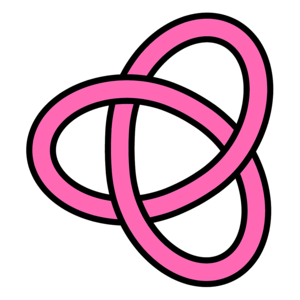
\includegraphics[width=\linewidth]{../data/knots/3_1.png}
        \subcaption{$3_{1}$}
    \end{minipage}
    \begin{minipage}[b]{.18\linewidth}
        \centering
        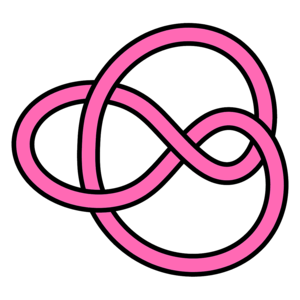
\includegraphics[width=\linewidth]{../data/knots/4_1.png}
        \subcaption{$4_{1}$}
    \end{minipage}
    \begin{minipage}[b]{.18\linewidth}
        \centering
        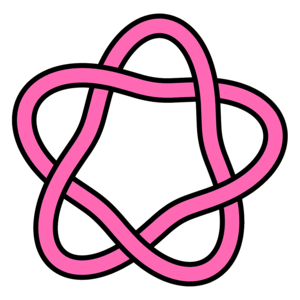
\includegraphics[width=\linewidth]{../data/knots/5_1.png}
        \subcaption{$5_{1}$}
    \end{minipage}
    \begin{minipage}[b]{.18\linewidth}
        \centering
        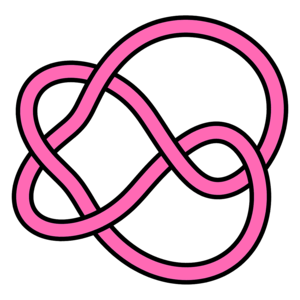
\includegraphics[width=\linewidth]{../data/knots/5_2.png}
        \subcaption{$5_{2}$}
    \end{minipage}
    \begin{minipage}[b]{.18\linewidth}
        \centering
        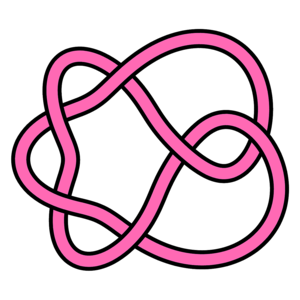
\includegraphics[width=\linewidth]{../data/knots/6_1.png}
        \subcaption{$6_{1}$}
    \end{minipage}
\end{figure}
\begin{figure}[H]
    \begin{minipage}[b]{.18\linewidth}
        \centering
        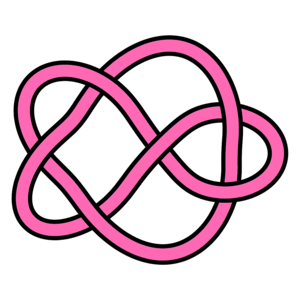
\includegraphics[width=\linewidth]{../data/knots/6_2.png}
        \subcaption{$6_{2}$}
    \end{minipage}
    \begin{minipage}[b]{.18\linewidth}
        \centering
        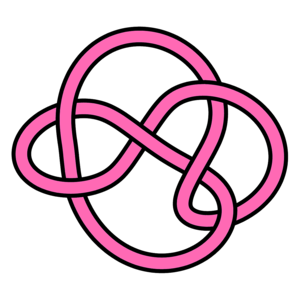
\includegraphics[width=\linewidth]{../data/knots/6_3.png}
        \subcaption{$6_{3}$}
    \end{minipage}
    \begin{minipage}[b]{.18\linewidth}
        \centering
        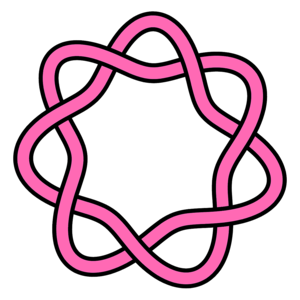
\includegraphics[width=\linewidth]{../data/knots/7_1.png}
        \subcaption{$7_{1}$}
    \end{minipage}
    \begin{minipage}[b]{.18\linewidth}
        \centering
        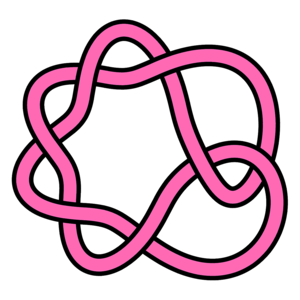
\includegraphics[width=\linewidth]{../data/knots/7_2.png}
        \subcaption{$7_{2}$}
    \end{minipage}
    \begin{minipage}[b]{.18\linewidth}
        \centering
        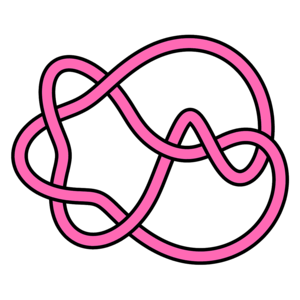
\includegraphics[width=\linewidth]{../data/knots/7_3.png}
        \subcaption{$7_{3}$}
    \end{minipage}
\end{figure}
\begin{figure}[H]
    \begin{minipage}[b]{.18\linewidth}
        \centering
        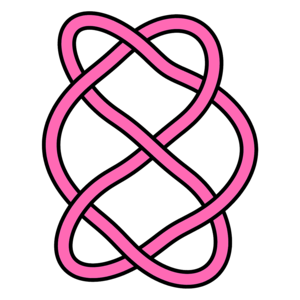
\includegraphics[width=\linewidth]{../data/knots/7_4.png}
        \subcaption{$7_{4}$}
    \end{minipage}
    \begin{minipage}[b]{.18\linewidth}
        \centering
        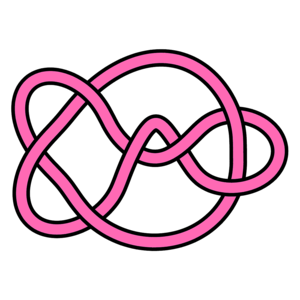
\includegraphics[width=\linewidth]{../data/knots/7_5.png}
        \subcaption{$7_{5}$}
    \end{minipage}
    \begin{minipage}[b]{.18\linewidth}
        \centering
        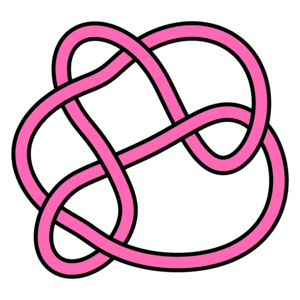
\includegraphics[width=\linewidth]{../data/knots/7_6.png}
        \subcaption{$7_{6}$}
    \end{minipage}
    \begin{minipage}[b]{.18\linewidth}
        \centering
        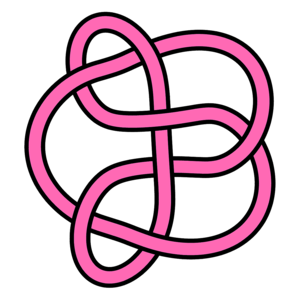
\includegraphics[width=\linewidth]{../data/knots/7_7.png}
        \subcaption{$7_{7}$}
    \end{minipage}
    \begin{minipage}[b]{.18\linewidth}
        \centering
        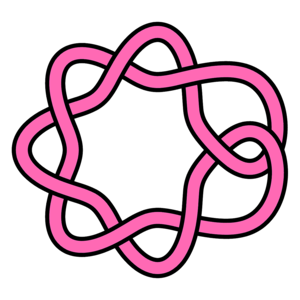
\includegraphics[width=\linewidth]{../data/knots/8_1.png}
        \subcaption{$8_{1}$}
    \end{minipage}
\end{figure}
\begin{figure}[H]
    \begin{minipage}[b]{.18\linewidth}
        \centering
        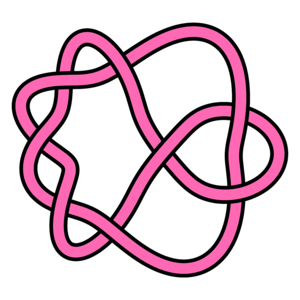
\includegraphics[width=\linewidth]{../data/knots/8_2.png}
        \subcaption{$8_{2}$}
    \end{minipage}
    \begin{minipage}[b]{.18\linewidth}
        \centering
        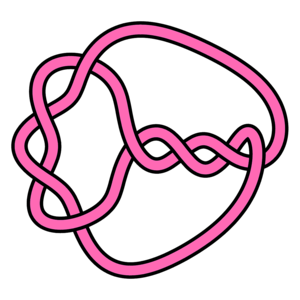
\includegraphics[width=\linewidth]{../data/knots/8_3.png}
        \subcaption{$8_{3}$}
    \end{minipage}
    \begin{minipage}[b]{.18\linewidth}
        \centering
        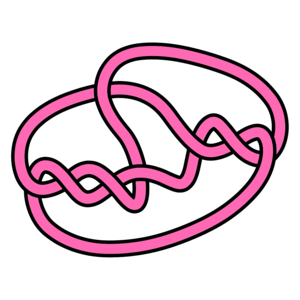
\includegraphics[width=\linewidth]{../data/knots/8_4.png}
        \subcaption{$8_{4}$}
    \end{minipage}
    \begin{minipage}[b]{.18\linewidth}
        \centering
        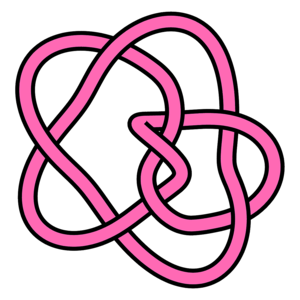
\includegraphics[width=\linewidth]{../data/knots/8_5.png}
        \subcaption{$8_{5}$}
    \end{minipage}
    \begin{minipage}[b]{.18\linewidth}
        \centering
        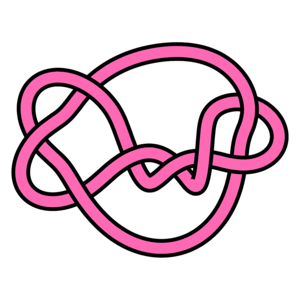
\includegraphics[width=\linewidth]{../data/knots/8_6.png}
        \subcaption{$8_{6}$}
    \end{minipage}
\end{figure}
\begin{figure}[H]
    \begin{minipage}[b]{.18\linewidth}
        \centering
        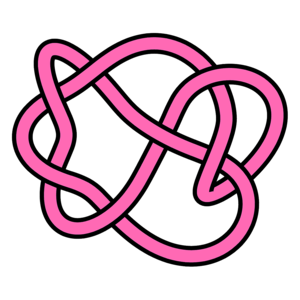
\includegraphics[width=\linewidth]{../data/knots/8_7.png}
        \subcaption{$8_{7}$}
    \end{minipage}
    \begin{minipage}[b]{.18\linewidth}
        \centering
        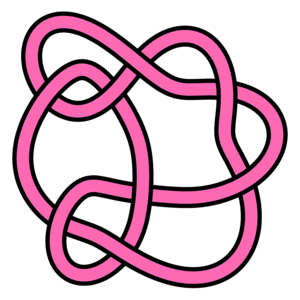
\includegraphics[width=\linewidth]{../data/knots/8_8.png}
        \subcaption{$8_{8}$}
    \end{minipage}
    \begin{minipage}[b]{.18\linewidth}
        \centering
        \includegraphics[width=\linewidth]{../data/knots/8_9.png}
        \subcaption{$8_{9}$}
    \end{minipage}
    \begin{minipage}[b]{.18\linewidth}
        \centering
        \includegraphics[width=\linewidth]{../data/knots/8_10.png}
        \subcaption{$8_{10}$}
    \end{minipage}
    \begin{minipage}[b]{.18\linewidth}
        \centering
        \includegraphics[width=\linewidth]{../data/knots/8_11.png}
        \subcaption{$8_{11}$}
    \end{minipage}
\end{figure}
\begin{figure}[H]
    \begin{minipage}[b]{.18\linewidth}
        \centering
        \includegraphics[width=\linewidth]{../data/knots/8_12.png}
        \subcaption{$8_{12}$}
    \end{minipage}
    \begin{minipage}[b]{.18\linewidth}
        \centering
        \includegraphics[width=\linewidth]{../data/knots/8_13.png}
        \subcaption{$8_{13}$}
    \end{minipage}
    \begin{minipage}[b]{.18\linewidth}
        \centering
        \includegraphics[width=\linewidth]{../data/knots/8_14.png}
        \subcaption{$8_{14}$}
    \end{minipage}
    \begin{minipage}[b]{.18\linewidth}
        \centering
        \includegraphics[width=\linewidth]{../data/knots/8_15.png}
        \subcaption{$8_{15}$}
    \end{minipage}
    \begin{minipage}[b]{.18\linewidth}
        \centering
        \includegraphics[width=\linewidth]{../data/knots/8_16.png}
        \subcaption{$8_{16}$}
    \end{minipage}
\end{figure}
\begin{figure}[H]
    \begin{minipage}[b]{.18\linewidth}
        \centering
        \includegraphics[width=\linewidth]{../data/knots/8_17.png}
        \subcaption{$8_{17}$}
    \end{minipage}
    \begin{minipage}[b]{.18\linewidth}
        \centering
        \includegraphics[width=\linewidth]{../data/knots/8_18.png}
        \subcaption{$8_{18}$}
    \end{minipage}
    \begin{minipage}[b]{.18\linewidth}
        \centering
        \includegraphics[width=\linewidth]{../data/knots/8_19.png}
        \subcaption{$8_{19}$}
    \end{minipage}
    \begin{minipage}[b]{.18\linewidth}
        \centering
        \includegraphics[width=\linewidth]{../data/knots/8_20.png}
        \subcaption{$8_{20}$}
    \end{minipage}
    \begin{minipage}[b]{.18\linewidth}
        \centering
        \includegraphics[width=\linewidth]{../data/knots/8_21.png}
        \subcaption{$8_{21}$}
    \end{minipage}
\end{figure}
\begin{figure}[H]
    \begin{minipage}[b]{.18\linewidth}
        \centering
        \includegraphics[width=\linewidth]{../data/knots/9_1.png}
        \subcaption{$9_{1}$}
    \end{minipage}
    \begin{minipage}[b]{.18\linewidth}
        \centering
        \includegraphics[width=\linewidth]{../data/knots/9_2.png}
        \subcaption{$9_{2}$}
    \end{minipage}
    \begin{minipage}[b]{.18\linewidth}
        \centering
        \includegraphics[width=\linewidth]{../data/knots/9_3.png}
        \subcaption{$9_{3}$}
    \end{minipage}
    \begin{minipage}[b]{.18\linewidth}
        \centering
        \includegraphics[width=\linewidth]{../data/knots/9_4.png}
        \subcaption{$9_{4}$}
    \end{minipage}
    \begin{minipage}[b]{.18\linewidth}
        \centering
        \includegraphics[width=\linewidth]{../data/knots/9_5.png}
        \subcaption{$9_{5}$}
    \end{minipage}
\end{figure}
\begin{figure}[H]
    \begin{minipage}[b]{.18\linewidth}
        \centering
        \includegraphics[width=\linewidth]{../data/knots/9_6.png}
        \subcaption{$9_{6}$}
    \end{minipage}
    \begin{minipage}[b]{.18\linewidth}
        \centering
        \includegraphics[width=\linewidth]{../data/knots/9_7.png}
        \subcaption{$9_{7}$}
    \end{minipage}
    \begin{minipage}[b]{.18\linewidth}
        \centering
        \includegraphics[width=\linewidth]{../data/knots/9_8.png}
        \subcaption{$9_{8}$}
    \end{minipage}
    \begin{minipage}[b]{.18\linewidth}
        \centering
        \includegraphics[width=\linewidth]{../data/knots/9_9.png}
        \subcaption{$9_{9}$}
    \end{minipage}
    \begin{minipage}[b]{.18\linewidth}
        \centering
        \includegraphics[width=\linewidth]{../data/knots/9_10.png}
        \subcaption{$9_{10}$}
    \end{minipage}
\end{figure}
\begin{figure}[H]
    \begin{minipage}[b]{.18\linewidth}
        \centering
        \includegraphics[width=\linewidth]{../data/knots/9_11.png}
        \subcaption{$9_{11}$}
    \end{minipage}
    \begin{minipage}[b]{.18\linewidth}
        \centering
        \includegraphics[width=\linewidth]{../data/knots/9_12.png}
        \subcaption{$9_{12}$}
    \end{minipage}
    \begin{minipage}[b]{.18\linewidth}
        \centering
        \includegraphics[width=\linewidth]{../data/knots/9_13.png}
        \subcaption{$9_{13}$}
    \end{minipage}
    \begin{minipage}[b]{.18\linewidth}
        \centering
        \includegraphics[width=\linewidth]{../data/knots/9_14.png}
        \subcaption{$9_{14}$}
    \end{minipage}
    \begin{minipage}[b]{.18\linewidth}
        \centering
        \includegraphics[width=\linewidth]{../data/knots/9_15.png}
        \subcaption{$9_{15}$}
    \end{minipage}
\end{figure}
\begin{figure}[H]
    \begin{minipage}[b]{.18\linewidth}
        \centering
        \includegraphics[width=\linewidth]{../data/knots/9_16.png}
        \subcaption{$9_{16}$}
    \end{minipage}
    \begin{minipage}[b]{.18\linewidth}
        \centering
        \includegraphics[width=\linewidth]{../data/knots/9_17.png}
        \subcaption{$9_{17}$}
    \end{minipage}
    \begin{minipage}[b]{.18\linewidth}
        \centering
        \includegraphics[width=\linewidth]{../data/knots/9_18.png}
        \subcaption{$9_{18}$}
    \end{minipage}
    \begin{minipage}[b]{.18\linewidth}
        \centering
        \includegraphics[width=\linewidth]{../data/knots/9_19.png}
        \subcaption{$9_{19}$}
    \end{minipage}
    \begin{minipage}[b]{.18\linewidth}
        \centering
        \includegraphics[width=\linewidth]{../data/knots/9_20.png}
        \subcaption{$9_{20}$}
    \end{minipage}
\end{figure}
\begin{figure}[H]
    \begin{minipage}[b]{.18\linewidth}
        \centering
        \includegraphics[width=\linewidth]{../data/knots/9_21.png}
        \subcaption{$9_{21}$}
    \end{minipage}
    \begin{minipage}[b]{.18\linewidth}
        \centering
        \includegraphics[width=\linewidth]{../data/knots/9_22.png}
        \subcaption{$9_{22}$}
    \end{minipage}
    \begin{minipage}[b]{.18\linewidth}
        \centering
        \includegraphics[width=\linewidth]{../data/knots/9_23.png}
        \subcaption{$9_{23}$}
    \end{minipage}
    \begin{minipage}[b]{.18\linewidth}
        \centering
        \includegraphics[width=\linewidth]{../data/knots/9_24.png}
        \subcaption{$9_{24}$}
    \end{minipage}
    \begin{minipage}[b]{.18\linewidth}
        \centering
        \includegraphics[width=\linewidth]{../data/knots/9_25.png}
        \subcaption{$9_{25}$}
    \end{minipage}
\end{figure}
\begin{figure}[H]
    \begin{minipage}[b]{.18\linewidth}
        \centering
        \includegraphics[width=\linewidth]{../data/knots/9_26.png}
        \subcaption{$9_{26}$}
    \end{minipage}
    \begin{minipage}[b]{.18\linewidth}
        \centering
        \includegraphics[width=\linewidth]{../data/knots/9_27.png}
        \subcaption{$9_{27}$}
    \end{minipage}
    \begin{minipage}[b]{.18\linewidth}
        \centering
        \includegraphics[width=\linewidth]{../data/knots/9_28.png}
        \subcaption{$9_{28}$}
    \end{minipage}
    \begin{minipage}[b]{.18\linewidth}
        \centering
        \includegraphics[width=\linewidth]{../data/knots/9_29.png}
        \subcaption{$9_{29}$}
    \end{minipage}
    \begin{minipage}[b]{.18\linewidth}
        \centering
        \includegraphics[width=\linewidth]{../data/knots/9_30.png}
        \subcaption{$9_{30}$}
    \end{minipage}
\end{figure}
\begin{figure}[H]
    \begin{minipage}[b]{.18\linewidth}
        \centering
        \includegraphics[width=\linewidth]{../data/knots/9_31.png}
        \subcaption{$9_{31}$}
    \end{minipage}
    \begin{minipage}[b]{.18\linewidth}
        \centering
        \includegraphics[width=\linewidth]{../data/knots/9_32.png}
        \subcaption{$9_{32}$}
    \end{minipage}
    \begin{minipage}[b]{.18\linewidth}
        \centering
        \includegraphics[width=\linewidth]{../data/knots/9_33.png}
        \subcaption{$9_{33}$}
    \end{minipage}
    \begin{minipage}[b]{.18\linewidth}
        \centering
        \includegraphics[width=\linewidth]{../data/knots/9_34.png}
        \subcaption{$9_{34}$}
    \end{minipage}
    \begin{minipage}[b]{.18\linewidth}
        \centering
        \includegraphics[width=\linewidth]{../data/knots/9_35.png}
        \subcaption{$9_{35}$}
    \end{minipage}
\end{figure}
\begin{figure}[H]
    \begin{minipage}[b]{.18\linewidth}
        \centering
        \includegraphics[width=\linewidth]{../data/knots/9_36.png}
        \subcaption{$9_{36}$}
    \end{minipage}
    \begin{minipage}[b]{.18\linewidth}
        \centering
        \includegraphics[width=\linewidth]{../data/knots/9_37.png}
        \subcaption{$9_{37}$}
    \end{minipage}
    \begin{minipage}[b]{.18\linewidth}
        \centering
        \includegraphics[width=\linewidth]{../data/knots/9_38.png}
        \subcaption{$9_{38}$}
    \end{minipage}
    \begin{minipage}[b]{.18\linewidth}
        \centering
        \includegraphics[width=\linewidth]{../data/knots/9_39.png}
        \subcaption{$9_{39}$}
    \end{minipage}
    \begin{minipage}[b]{.18\linewidth}
        \centering
        \includegraphics[width=\linewidth]{../data/knots/9_40.png}
        \subcaption{$9_{40}$}
    \end{minipage}
\end{figure}
\begin{figure}[H]
    \begin{minipage}[b]{.18\linewidth}
        \centering
        \includegraphics[width=\linewidth]{../data/knots/9_41.png}
        \subcaption{$9_{41}$}
    \end{minipage}
    \begin{minipage}[b]{.18\linewidth}
        \centering
        \includegraphics[width=\linewidth]{../data/knots/9_42.png}
        \subcaption{$9_{42}$}
    \end{minipage}
    \begin{minipage}[b]{.18\linewidth}
        \centering
        \includegraphics[width=\linewidth]{../data/knots/9_43.png}
        \subcaption{$9_{43}$}
    \end{minipage}
    \begin{minipage}[b]{.18\linewidth}
        \centering
        \includegraphics[width=\linewidth]{../data/knots/9_44.png}
        \subcaption{$9_{44}$}
    \end{minipage}
    \begin{minipage}[b]{.18\linewidth}
        \centering
        \includegraphics[width=\linewidth]{../data/knots/9_45.png}
        \subcaption{$9_{45}$}
    \end{minipage}
\end{figure}
\begin{figure}[H]
    \begin{minipage}[b]{.18\linewidth}
        \centering
        \includegraphics[width=\linewidth]{../data/knots/9_46.png}
        \subcaption{$9_{46}$}
    \end{minipage}
    \begin{minipage}[b]{.18\linewidth}
        \centering
        \includegraphics[width=\linewidth]{../data/knots/9_47.png}
        \subcaption{$9_{47}$}
    \end{minipage}
    \begin{minipage}[b]{.18\linewidth}
        \centering
        \includegraphics[width=\linewidth]{../data/knots/9_48.png}
        \subcaption{$9_{48}$}
    \end{minipage}
    \begin{minipage}[b]{.18\linewidth}
        \centering
        \includegraphics[width=\linewidth]{../data/knots/9_49.png}
        \subcaption{$9_{49}$}
    \end{minipage}
    \begin{minipage}[b]{.18\linewidth}
        \centering
        \includegraphics[width=\linewidth]{../data/knots/10_1.png}
        \subcaption{$10_{1}$}
    \end{minipage}
\end{figure}
\begin{figure}[H]
    \begin{minipage}[b]{.18\linewidth}
        \centering
        \includegraphics[width=\linewidth]{../data/knots/10_2.png}
        \subcaption{$10_{2}$}
    \end{minipage}
    \begin{minipage}[b]{.18\linewidth}
        \centering
        \includegraphics[width=\linewidth]{../data/knots/10_3.png}
        \subcaption{$10_{3}$}
    \end{minipage}
    \begin{minipage}[b]{.18\linewidth}
        \centering
        \includegraphics[width=\linewidth]{../data/knots/10_4.png}
        \subcaption{$10_{4}$}
    \end{minipage}
    \begin{minipage}[b]{.18\linewidth}
        \centering
        \includegraphics[width=\linewidth]{../data/knots/10_5.png}
        \subcaption{$10_{5}$}
    \end{minipage}
    \begin{minipage}[b]{.18\linewidth}
        \centering
        \includegraphics[width=\linewidth]{../data/knots/10_6.png}
        \subcaption{$10_{6}$}
    \end{minipage}
\end{figure}
\begin{figure}[H]
    \begin{minipage}[b]{.18\linewidth}
        \centering
        \includegraphics[width=\linewidth]{../data/knots/10_7.png}
        \subcaption{$10_{7}$}
    \end{minipage}
    \begin{minipage}[b]{.18\linewidth}
        \centering
        \includegraphics[width=\linewidth]{../data/knots/10_8.png}
        \subcaption{$10_{8}$}
    \end{minipage}
    \begin{minipage}[b]{.18\linewidth}
        \centering
        \includegraphics[width=\linewidth]{../data/knots/10_9.png}
        \subcaption{$10_{9}$}
    \end{minipage}
    \begin{minipage}[b]{.18\linewidth}
        \centering
        \includegraphics[width=\linewidth]{../data/knots/10_10.png}
        \subcaption{$10_{10}$}
    \end{minipage}
    \begin{minipage}[b]{.18\linewidth}
        \centering
        \includegraphics[width=\linewidth]{../data/knots/10_11.png}
        \subcaption{$10_{11}$}
    \end{minipage}
\end{figure}
\begin{figure}[H]
    \begin{minipage}[b]{.18\linewidth}
        \centering
        \includegraphics[width=\linewidth]{../data/knots/10_12.png}
        \subcaption{$10_{12}$}
    \end{minipage}
    \begin{minipage}[b]{.18\linewidth}
        \centering
        \includegraphics[width=\linewidth]{../data/knots/10_13.png}
        \subcaption{$10_{13}$}
    \end{minipage}
    \begin{minipage}[b]{.18\linewidth}
        \centering
        \includegraphics[width=\linewidth]{../data/knots/10_14.png}
        \subcaption{$10_{14}$}
    \end{minipage}
    \begin{minipage}[b]{.18\linewidth}
        \centering
        \includegraphics[width=\linewidth]{../data/knots/10_15.png}
        \subcaption{$10_{15}$}
    \end{minipage}
    \begin{minipage}[b]{.18\linewidth}
        \centering
        \includegraphics[width=\linewidth]{../data/knots/10_16.png}
        \subcaption{$10_{16}$}
    \end{minipage}
\end{figure}
\begin{figure}[H]
    \begin{minipage}[b]{.18\linewidth}
        \centering
        \includegraphics[width=\linewidth]{../data/knots/10_17.png}
        \subcaption{$10_{17}$}
    \end{minipage}
    \begin{minipage}[b]{.18\linewidth}
        \centering
        \includegraphics[width=\linewidth]{../data/knots/10_18.png}
        \subcaption{$10_{18}$}
    \end{minipage}
    \begin{minipage}[b]{.18\linewidth}
        \centering
        \includegraphics[width=\linewidth]{../data/knots/10_19.png}
        \subcaption{$10_{19}$}
    \end{minipage}
    \begin{minipage}[b]{.18\linewidth}
        \centering
        \includegraphics[width=\linewidth]{../data/knots/10_20.png}
        \subcaption{$10_{20}$}
    \end{minipage}
    \begin{minipage}[b]{.18\linewidth}
        \centering
        \includegraphics[width=\linewidth]{../data/knots/10_21.png}
        \subcaption{$10_{21}$}
    \end{minipage}
\end{figure}
\begin{figure}[H]
    \begin{minipage}[b]{.18\linewidth}
        \centering
        \includegraphics[width=\linewidth]{../data/knots/10_22.png}
        \subcaption{$10_{22}$}
    \end{minipage}
    \begin{minipage}[b]{.18\linewidth}
        \centering
        \includegraphics[width=\linewidth]{../data/knots/10_23.png}
        \subcaption{$10_{23}$}
    \end{minipage}
    \begin{minipage}[b]{.18\linewidth}
        \centering
        \includegraphics[width=\linewidth]{../data/knots/10_24.png}
        \subcaption{$10_{24}$}
    \end{minipage}
    \begin{minipage}[b]{.18\linewidth}
        \centering
        \includegraphics[width=\linewidth]{../data/knots/10_25.png}
        \subcaption{$10_{25}$}
    \end{minipage}
    \begin{minipage}[b]{.18\linewidth}
        \centering
        \includegraphics[width=\linewidth]{../data/knots/10_26.png}
        \subcaption{$10_{26}$}
    \end{minipage}
\end{figure}
\begin{figure}[H]
    \begin{minipage}[b]{.18\linewidth}
        \centering
        \includegraphics[width=\linewidth]{../data/knots/10_27.png}
        \subcaption{$10_{27}$}
    \end{minipage}
    \begin{minipage}[b]{.18\linewidth}
        \centering
        \includegraphics[width=\linewidth]{../data/knots/10_28.png}
        \subcaption{$10_{28}$}
    \end{minipage}
    \begin{minipage}[b]{.18\linewidth}
        \centering
        \includegraphics[width=\linewidth]{../data/knots/10_29.png}
        \subcaption{$10_{29}$}
    \end{minipage}
    \begin{minipage}[b]{.18\linewidth}
        \centering
        \includegraphics[width=\linewidth]{../data/knots/10_30.png}
        \subcaption{$10_{30}$}
    \end{minipage}
    \begin{minipage}[b]{.18\linewidth}
        \centering
        \includegraphics[width=\linewidth]{../data/knots/10_31.png}
        \subcaption{$10_{31}$}
    \end{minipage}
\end{figure}
\begin{figure}[H]
    \begin{minipage}[b]{.18\linewidth}
        \centering
        \includegraphics[width=\linewidth]{../data/knots/10_32.png}
        \subcaption{$10_{32}$}
    \end{minipage}
    \begin{minipage}[b]{.18\linewidth}
        \centering
        \includegraphics[width=\linewidth]{../data/knots/10_33.png}
        \subcaption{$10_{33}$}
    \end{minipage}
    \begin{minipage}[b]{.18\linewidth}
        \centering
        \includegraphics[width=\linewidth]{../data/knots/10_34.png}
        \subcaption{$10_{34}$}
    \end{minipage}
    \begin{minipage}[b]{.18\linewidth}
        \centering
        \includegraphics[width=\linewidth]{../data/knots/10_35.png}
        \subcaption{$10_{35}$}
    \end{minipage}
    \begin{minipage}[b]{.18\linewidth}
        \centering
        \includegraphics[width=\linewidth]{../data/knots/10_36.png}
        \subcaption{$10_{36}$}
    \end{minipage}
\end{figure}
\begin{figure}[H]
    \begin{minipage}[b]{.18\linewidth}
        \centering
        \includegraphics[width=\linewidth]{../data/knots/10_37.png}
        \subcaption{$10_{37}$}
    \end{minipage}
    \begin{minipage}[b]{.18\linewidth}
        \centering
        \includegraphics[width=\linewidth]{../data/knots/10_38.png}
        \subcaption{$10_{38}$}
    \end{minipage}
    \begin{minipage}[b]{.18\linewidth}
        \centering
        \includegraphics[width=\linewidth]{../data/knots/10_39.png}
        \subcaption{$10_{39}$}
    \end{minipage}
    \begin{minipage}[b]{.18\linewidth}
        \centering
        \includegraphics[width=\linewidth]{../data/knots/10_40.png}
        \subcaption{$10_{40}$}
    \end{minipage}
    \begin{minipage}[b]{.18\linewidth}
        \centering
        \includegraphics[width=\linewidth]{../data/knots/10_41.png}
        \subcaption{$10_{41}$}
    \end{minipage}
\end{figure}
\begin{figure}[H]
    \begin{minipage}[b]{.18\linewidth}
        \centering
        \includegraphics[width=\linewidth]{../data/knots/10_42.png}
        \subcaption{$10_{42}$}
    \end{minipage}
    \begin{minipage}[b]{.18\linewidth}
        \centering
        \includegraphics[width=\linewidth]{../data/knots/10_43.png}
        \subcaption{$10_{43}$}
    \end{minipage}
    \begin{minipage}[b]{.18\linewidth}
        \centering
        \includegraphics[width=\linewidth]{../data/knots/10_44.png}
        \subcaption{$10_{44}$}
    \end{minipage}
    \begin{minipage}[b]{.18\linewidth}
        \centering
        \includegraphics[width=\linewidth]{../data/knots/10_45.png}
        \subcaption{$10_{45}$}
    \end{minipage}
    \begin{minipage}[b]{.18\linewidth}
        \centering
        \includegraphics[width=\linewidth]{../data/knots/10_46.png}
        \subcaption{$10_{46}$}
    \end{minipage}
\end{figure}
\begin{figure}[H]
    \begin{minipage}[b]{.18\linewidth}
        \centering
        \includegraphics[width=\linewidth]{../data/knots/10_47.png}
        \subcaption{$10_{47}$}
    \end{minipage}
    \begin{minipage}[b]{.18\linewidth}
        \centering
        \includegraphics[width=\linewidth]{../data/knots/10_48.png}
        \subcaption{$10_{48}$}
    \end{minipage}
    \begin{minipage}[b]{.18\linewidth}
        \centering
        \includegraphics[width=\linewidth]{../data/knots/10_49.png}
        \subcaption{$10_{49}$}
    \end{minipage}
    \begin{minipage}[b]{.18\linewidth}
        \centering
        \includegraphics[width=\linewidth]{../data/knots/10_50.png}
        \subcaption{$10_{50}$}
    \end{minipage}
    \begin{minipage}[b]{.18\linewidth}
        \centering
        \includegraphics[width=\linewidth]{../data/knots/10_51.png}
        \subcaption{$10_{51}$}
    \end{minipage}
\end{figure}
\begin{figure}[H]
    \begin{minipage}[b]{.18\linewidth}
        \centering
        \includegraphics[width=\linewidth]{../data/knots/10_52.png}
        \subcaption{$10_{52}$}
    \end{minipage}
    \begin{minipage}[b]{.18\linewidth}
        \centering
        \includegraphics[width=\linewidth]{../data/knots/10_53.png}
        \subcaption{$10_{53}$}
    \end{minipage}
    \begin{minipage}[b]{.18\linewidth}
        \centering
        \includegraphics[width=\linewidth]{../data/knots/10_54.png}
        \subcaption{$10_{54}$}
    \end{minipage}
    \begin{minipage}[b]{.18\linewidth}
        \centering
        \includegraphics[width=\linewidth]{../data/knots/10_55.png}
        \subcaption{$10_{55}$}
    \end{minipage}
    \begin{minipage}[b]{.18\linewidth}
        \centering
        \includegraphics[width=\linewidth]{../data/knots/10_56.png}
        \subcaption{$10_{56}$}
    \end{minipage}
\end{figure}
\begin{figure}[H]
    \begin{minipage}[b]{.18\linewidth}
        \centering
        \includegraphics[width=\linewidth]{../data/knots/10_57.png}
        \subcaption{$10_{57}$}
    \end{minipage}
    \begin{minipage}[b]{.18\linewidth}
        \centering
        \includegraphics[width=\linewidth]{../data/knots/10_58.png}
        \subcaption{$10_{58}$}
    \end{minipage}
    \begin{minipage}[b]{.18\linewidth}
        \centering
        \includegraphics[width=\linewidth]{../data/knots/10_59.png}
        \subcaption{$10_{59}$}
    \end{minipage}
    \begin{minipage}[b]{.18\linewidth}
        \centering
        \includegraphics[width=\linewidth]{../data/knots/10_60.png}
        \subcaption{$10_{60}$}
    \end{minipage}
    \begin{minipage}[b]{.18\linewidth}
        \centering
        \includegraphics[width=\linewidth]{../data/knots/10_61.png}
        \subcaption{$10_{61}$}
    \end{minipage}
\end{figure}
\begin{figure}[H]
    \begin{minipage}[b]{.18\linewidth}
        \centering
        \includegraphics[width=\linewidth]{../data/knots/10_62.png}
        \subcaption{$10_{62}$}
    \end{minipage}
    \begin{minipage}[b]{.18\linewidth}
        \centering
        \includegraphics[width=\linewidth]{../data/knots/10_63.png}
        \subcaption{$10_{63}$}
    \end{minipage}
    \begin{minipage}[b]{.18\linewidth}
        \centering
        \includegraphics[width=\linewidth]{../data/knots/10_64.png}
        \subcaption{$10_{64}$}
    \end{minipage}
    \begin{minipage}[b]{.18\linewidth}
        \centering
        \includegraphics[width=\linewidth]{../data/knots/10_65.png}
        \subcaption{$10_{65}$}
    \end{minipage}
    \begin{minipage}[b]{.18\linewidth}
        \centering
        \includegraphics[width=\linewidth]{../data/knots/10_66.png}
        \subcaption{$10_{66}$}
    \end{minipage}
\end{figure}
\begin{figure}[H]
    \begin{minipage}[b]{.18\linewidth}
        \centering
        \includegraphics[width=\linewidth]{../data/knots/10_67.png}
        \subcaption{$10_{67}$}
    \end{minipage}
    \begin{minipage}[b]{.18\linewidth}
        \centering
        \includegraphics[width=\linewidth]{../data/knots/10_68.png}
        \subcaption{$10_{68}$}
    \end{minipage}
    \begin{minipage}[b]{.18\linewidth}
        \centering
        \includegraphics[width=\linewidth]{../data/knots/10_69.png}
        \subcaption{$10_{69}$}
    \end{minipage}
    \begin{minipage}[b]{.18\linewidth}
        \centering
        \includegraphics[width=\linewidth]{../data/knots/10_70.png}
        \subcaption{$10_{70}$}
    \end{minipage}
    \begin{minipage}[b]{.18\linewidth}
        \centering
        \includegraphics[width=\linewidth]{../data/knots/10_71.png}
        \subcaption{$10_{71}$}
    \end{minipage}
\end{figure}
\begin{figure}[H]
    \begin{minipage}[b]{.18\linewidth}
        \centering
        \includegraphics[width=\linewidth]{../data/knots/10_72.png}
        \subcaption{$10_{72}$}
    \end{minipage}
    \begin{minipage}[b]{.18\linewidth}
        \centering
        \includegraphics[width=\linewidth]{../data/knots/10_73.png}
        \subcaption{$10_{73}$}
    \end{minipage}
    \begin{minipage}[b]{.18\linewidth}
        \centering
        \includegraphics[width=\linewidth]{../data/knots/10_74.png}
        \subcaption{$10_{74}$}
    \end{minipage}
    \begin{minipage}[b]{.18\linewidth}
        \centering
        \includegraphics[width=\linewidth]{../data/knots/10_75.png}
        \subcaption{$10_{75}$}
    \end{minipage}
    \begin{minipage}[b]{.18\linewidth}
        \centering
        \includegraphics[width=\linewidth]{../data/knots/10_76.png}
        \subcaption{$10_{76}$}
    \end{minipage}
\end{figure}
\begin{figure}[H]
    \begin{minipage}[b]{.18\linewidth}
        \centering
        \includegraphics[width=\linewidth]{../data/knots/10_77.png}
        \subcaption{$10_{77}$}
    \end{minipage}
    \begin{minipage}[b]{.18\linewidth}
        \centering
        \includegraphics[width=\linewidth]{../data/knots/10_78.png}
        \subcaption{$10_{78}$}
    \end{minipage}
    \begin{minipage}[b]{.18\linewidth}
        \centering
        \includegraphics[width=\linewidth]{../data/knots/10_79.png}
        \subcaption{$10_{79}$}
    \end{minipage}
    \begin{minipage}[b]{.18\linewidth}
        \centering
        \includegraphics[width=\linewidth]{../data/knots/10_80.png}
        \subcaption{$10_{80}$}
    \end{minipage}
    \begin{minipage}[b]{.18\linewidth}
        \centering
        \includegraphics[width=\linewidth]{../data/knots/10_81.png}
        \subcaption{$10_{81}$}
    \end{minipage}
\end{figure}
\begin{figure}[H]
    \begin{minipage}[b]{.18\linewidth}
        \centering
        \includegraphics[width=\linewidth]{../data/knots/10_82.png}
        \subcaption{$10_{82}$}
    \end{minipage}
    \begin{minipage}[b]{.18\linewidth}
        \centering
        \includegraphics[width=\linewidth]{../data/knots/10_83.png}
        \subcaption{$10_{83}$}
    \end{minipage}
    \begin{minipage}[b]{.18\linewidth}
        \centering
        \includegraphics[width=\linewidth]{../data/knots/10_84.png}
        \subcaption{$10_{84}$}
    \end{minipage}
    \begin{minipage}[b]{.18\linewidth}
        \centering
        \includegraphics[width=\linewidth]{../data/knots/10_85.png}
        \subcaption{$10_{85}$}
    \end{minipage}
    \begin{minipage}[b]{.18\linewidth}
        \centering
        \includegraphics[width=\linewidth]{../data/knots/10_86.png}
        \subcaption{$10_{86}$}
    \end{minipage}
\end{figure}
\begin{figure}[H]
    \begin{minipage}[b]{.18\linewidth}
        \centering
        \includegraphics[width=\linewidth]{../data/knots/10_87.png}
        \subcaption{$10_{87}$}
    \end{minipage}
    \begin{minipage}[b]{.18\linewidth}
        \centering
        \includegraphics[width=\linewidth]{../data/knots/10_88.png}
        \subcaption{$10_{88}$}
    \end{minipage}
    \begin{minipage}[b]{.18\linewidth}
        \centering
        \includegraphics[width=\linewidth]{../data/knots/10_89.png}
        \subcaption{$10_{89}$}
    \end{minipage}
    \begin{minipage}[b]{.18\linewidth}
        \centering
        \includegraphics[width=\linewidth]{../data/knots/10_90.png}
        \subcaption{$10_{90}$}
    \end{minipage}
    \begin{minipage}[b]{.18\linewidth}
        \centering
        \includegraphics[width=\linewidth]{../data/knots/10_91.png}
        \subcaption{$10_{91}$}
    \end{minipage}
\end{figure}
\begin{figure}[H]
    \begin{minipage}[b]{.18\linewidth}
        \centering
        \includegraphics[width=\linewidth]{../data/knots/10_92.png}
        \subcaption{$10_{92}$}
    \end{minipage}
    \begin{minipage}[b]{.18\linewidth}
        \centering
        \includegraphics[width=\linewidth]{../data/knots/10_93.png}
        \subcaption{$10_{93}$}
    \end{minipage}
    \begin{minipage}[b]{.18\linewidth}
        \centering
        \includegraphics[width=\linewidth]{../data/knots/10_94.png}
        \subcaption{$10_{94}$}
    \end{minipage}
    \begin{minipage}[b]{.18\linewidth}
        \centering
        \includegraphics[width=\linewidth]{../data/knots/10_95.png}
        \subcaption{$10_{95}$}
    \end{minipage}
    \begin{minipage}[b]{.18\linewidth}
        \centering
        \includegraphics[width=\linewidth]{../data/knots/10_96.png}
        \subcaption{$10_{96}$}
    \end{minipage}
\end{figure}
\begin{figure}[H]
    \begin{minipage}[b]{.18\linewidth}
        \centering
        \includegraphics[width=\linewidth]{../data/knots/10_97.png}
        \subcaption{$10_{97}$}
    \end{minipage}
    \begin{minipage}[b]{.18\linewidth}
        \centering
        \includegraphics[width=\linewidth]{../data/knots/10_98.png}
        \subcaption{$10_{98}$}
    \end{minipage}
    \begin{minipage}[b]{.18\linewidth}
        \centering
        \includegraphics[width=\linewidth]{../data/knots/10_99.png}
        \subcaption{$10_{99}$}
    \end{minipage}
    \begin{minipage}[b]{.18\linewidth}
        \centering
        \includegraphics[width=\linewidth]{../data/knots/10_100.png}
        \subcaption{$10_{100}$}
    \end{minipage}
    \begin{minipage}[b]{.18\linewidth}
        \centering
        \includegraphics[width=\linewidth]{../data/knots/10_101.png}
        \subcaption{$10_{101}$}
    \end{minipage}
\end{figure}
\begin{figure}[H]
    \begin{minipage}[b]{.18\linewidth}
        \centering
        \includegraphics[width=\linewidth]{../data/knots/10_102.png}
        \subcaption{$10_{102}$}
    \end{minipage}
    \begin{minipage}[b]{.18\linewidth}
        \centering
        \includegraphics[width=\linewidth]{../data/knots/10_103.png}
        \subcaption{$10_{103}$}
    \end{minipage}
    \begin{minipage}[b]{.18\linewidth}
        \centering
        \includegraphics[width=\linewidth]{../data/knots/10_104.png}
        \subcaption{$10_{104}$}
    \end{minipage}
    \begin{minipage}[b]{.18\linewidth}
        \centering
        \includegraphics[width=\linewidth]{../data/knots/10_105.png}
        \subcaption{$10_{105}$}
    \end{minipage}
    \begin{minipage}[b]{.18\linewidth}
        \centering
        \includegraphics[width=\linewidth]{../data/knots/10_106.png}
        \subcaption{$10_{106}$}
    \end{minipage}
\end{figure}
\begin{figure}[H]
    \begin{minipage}[b]{.18\linewidth}
        \centering
        \includegraphics[width=\linewidth]{../data/knots/10_107.png}
        \subcaption{$10_{107}$}
    \end{minipage}
    \begin{minipage}[b]{.18\linewidth}
        \centering
        \includegraphics[width=\linewidth]{../data/knots/10_108.png}
        \subcaption{$10_{108}$}
    \end{minipage}
    \begin{minipage}[b]{.18\linewidth}
        \centering
        \includegraphics[width=\linewidth]{../data/knots/10_109.png}
        \subcaption{$10_{109}$}
    \end{minipage}
    \begin{minipage}[b]{.18\linewidth}
        \centering
        \includegraphics[width=\linewidth]{../data/knots/10_110.png}
        \subcaption{$10_{110}$}
    \end{minipage}
    \begin{minipage}[b]{.18\linewidth}
        \centering
        \includegraphics[width=\linewidth]{../data/knots/10_111.png}
        \subcaption{$10_{111}$}
    \end{minipage}
\end{figure}
\begin{figure}[H]
    \begin{minipage}[b]{.18\linewidth}
        \centering
        \includegraphics[width=\linewidth]{../data/knots/10_112.png}
        \subcaption{$10_{112}$}
    \end{minipage}
    \begin{minipage}[b]{.18\linewidth}
        \centering
        \includegraphics[width=\linewidth]{../data/knots/10_113.png}
        \subcaption{$10_{113}$}
    \end{minipage}
    \begin{minipage}[b]{.18\linewidth}
        \centering
        \includegraphics[width=\linewidth]{../data/knots/10_114.png}
        \subcaption{$10_{114}$}
    \end{minipage}
    \begin{minipage}[b]{.18\linewidth}
        \centering
        \includegraphics[width=\linewidth]{../data/knots/10_115.png}
        \subcaption{$10_{115}$}
    \end{minipage}
    \begin{minipage}[b]{.18\linewidth}
        \centering
        \includegraphics[width=\linewidth]{../data/knots/10_116.png}
        \subcaption{$10_{116}$}
    \end{minipage}
\end{figure}
\begin{figure}[H]
    \begin{minipage}[b]{.18\linewidth}
        \centering
        \includegraphics[width=\linewidth]{../data/knots/10_117.png}
        \subcaption{$10_{117}$}
    \end{minipage}
    \begin{minipage}[b]{.18\linewidth}
        \centering
        \includegraphics[width=\linewidth]{../data/knots/10_118.png}
        \subcaption{$10_{118}$}
    \end{minipage}
    \begin{minipage}[b]{.18\linewidth}
        \centering
        \includegraphics[width=\linewidth]{../data/knots/10_119.png}
        \subcaption{$10_{119}$}
    \end{minipage}
    \begin{minipage}[b]{.18\linewidth}
        \centering
        \includegraphics[width=\linewidth]{../data/knots/10_120.png}
        \subcaption{$10_{120}$}
    \end{minipage}
    \begin{minipage}[b]{.18\linewidth}
        \centering
        \includegraphics[width=\linewidth]{../data/knots/10_121.png}
        \subcaption{$10_{121}$}
    \end{minipage}
\end{figure}
\begin{figure}[H]
    \begin{minipage}[b]{.18\linewidth}
        \centering
        \includegraphics[width=\linewidth]{../data/knots/10_122.png}
        \subcaption{$10_{122}$}
    \end{minipage}
    \begin{minipage}[b]{.18\linewidth}
        \centering
        \includegraphics[width=\linewidth]{../data/knots/10_123.png}
        \subcaption{$10_{123}$}
    \end{minipage}
    \begin{minipage}[b]{.18\linewidth}
        \centering
        \includegraphics[width=\linewidth]{../data/knots/10_124.png}
        \subcaption{$10_{124}$}
    \end{minipage}
    \begin{minipage}[b]{.18\linewidth}
        \centering
        \includegraphics[width=\linewidth]{../data/knots/10_125.png}
        \subcaption{$10_{125}$}
    \end{minipage}
    \begin{minipage}[b]{.18\linewidth}
        \centering
        \includegraphics[width=\linewidth]{../data/knots/10_126.png}
        \subcaption{$10_{126}$}
    \end{minipage}
\end{figure}
\begin{figure}[H]
    \begin{minipage}[b]{.18\linewidth}
        \centering
        \includegraphics[width=\linewidth]{../data/knots/10_127.png}
        \subcaption{$10_{127}$}
    \end{minipage}
    \begin{minipage}[b]{.18\linewidth}
        \centering
        \includegraphics[width=\linewidth]{../data/knots/10_128.png}
        \subcaption{$10_{128}$}
    \end{minipage}
    \begin{minipage}[b]{.18\linewidth}
        \centering
        \includegraphics[width=\linewidth]{../data/knots/10_129.png}
        \subcaption{$10_{129}$}
    \end{minipage}
    \begin{minipage}[b]{.18\linewidth}
        \centering
        \includegraphics[width=\linewidth]{../data/knots/10_130.png}
        \subcaption{$10_{130}$}
    \end{minipage}
    \begin{minipage}[b]{.18\linewidth}
        \centering
        \includegraphics[width=\linewidth]{../data/knots/10_131.png}
        \subcaption{$10_{131}$}
    \end{minipage}
\end{figure}
\begin{figure}[H]
    \begin{minipage}[b]{.18\linewidth}
        \centering
        \includegraphics[width=\linewidth]{../data/knots/10_132.png}
        \subcaption{$10_{132}$}
    \end{minipage}
    \begin{minipage}[b]{.18\linewidth}
        \centering
        \includegraphics[width=\linewidth]{../data/knots/10_133.png}
        \subcaption{$10_{133}$}
    \end{minipage}
    \begin{minipage}[b]{.18\linewidth}
        \centering
        \includegraphics[width=\linewidth]{../data/knots/10_134.png}
        \subcaption{$10_{134}$}
    \end{minipage}
    \begin{minipage}[b]{.18\linewidth}
        \centering
        \includegraphics[width=\linewidth]{../data/knots/10_135.png}
        \subcaption{$10_{135}$}
    \end{minipage}
    \begin{minipage}[b]{.18\linewidth}
        \centering
        \includegraphics[width=\linewidth]{../data/knots/10_136.png}
        \subcaption{$10_{136}$}
    \end{minipage}
\end{figure}
\begin{figure}[H]
    \begin{minipage}[b]{.18\linewidth}
        \centering
        \includegraphics[width=\linewidth]{../data/knots/10_137.png}
        \subcaption{$10_{137}$}
    \end{minipage}
    \begin{minipage}[b]{.18\linewidth}
        \centering
        \includegraphics[width=\linewidth]{../data/knots/10_138.png}
        \subcaption{$10_{138}$}
    \end{minipage}
    \begin{minipage}[b]{.18\linewidth}
        \centering
        \includegraphics[width=\linewidth]{../data/knots/10_139.png}
        \subcaption{$10_{139}$}
    \end{minipage}
    \begin{minipage}[b]{.18\linewidth}
        \centering
        \includegraphics[width=\linewidth]{../data/knots/10_140.png}
        \subcaption{$10_{140}$}
    \end{minipage}
    \begin{minipage}[b]{.18\linewidth}
        \centering
        \includegraphics[width=\linewidth]{../data/knots/10_141.png}
        \subcaption{$10_{141}$}
    \end{minipage}
\end{figure}
\begin{figure}[H]
    \begin{minipage}[b]{.18\linewidth}
        \centering
        \includegraphics[width=\linewidth]{../data/knots/10_142.png}
        \subcaption{$10_{142}$}
    \end{minipage}
    \begin{minipage}[b]{.18\linewidth}
        \centering
        \includegraphics[width=\linewidth]{../data/knots/10_143.png}
        \subcaption{$10_{143}$}
    \end{minipage}
    \begin{minipage}[b]{.18\linewidth}
        \centering
        \includegraphics[width=\linewidth]{../data/knots/10_144.png}
        \subcaption{$10_{144}$}
    \end{minipage}
    \begin{minipage}[b]{.18\linewidth}
        \centering
        \includegraphics[width=\linewidth]{../data/knots/10_145.png}
        \subcaption{$10_{145}$}
    \end{minipage}
    \begin{minipage}[b]{.18\linewidth}
        \centering
        \includegraphics[width=\linewidth]{../data/knots/10_146.png}
        \subcaption{$10_{146}$}
    \end{minipage}
\end{figure}
\begin{figure}[H]
    \begin{minipage}[b]{.18\linewidth}
        \centering
        \includegraphics[width=\linewidth]{../data/knots/10_147.png}
        \subcaption{$10_{147}$}
    \end{minipage}
    \begin{minipage}[b]{.18\linewidth}
        \centering
        \includegraphics[width=\linewidth]{../data/knots/10_148.png}
        \subcaption{$10_{148}$}
    \end{minipage}
    \begin{minipage}[b]{.18\linewidth}
        \centering
        \includegraphics[width=\linewidth]{../data/knots/10_149.png}
        \subcaption{$10_{149}$}
    \end{minipage}
    \begin{minipage}[b]{.18\linewidth}
        \centering
        \includegraphics[width=\linewidth]{../data/knots/10_150.png}
        \subcaption{$10_{150}$}
    \end{minipage}
    \begin{minipage}[b]{.18\linewidth}
        \centering
        \includegraphics[width=\linewidth]{../data/knots/10_151.png}
        \subcaption{$10_{151}$}
    \end{minipage}
\end{figure}
\begin{figure}[H]
    \begin{minipage}[b]{.18\linewidth}
        \centering
        \includegraphics[width=\linewidth]{../data/knots/10_152.png}
        \subcaption{$10_{152}$}
    \end{minipage}
    \begin{minipage}[b]{.18\linewidth}
        \centering
        \includegraphics[width=\linewidth]{../data/knots/10_153.png}
        \subcaption{$10_{153}$}
    \end{minipage}
    \begin{minipage}[b]{.18\linewidth}
        \centering
        \includegraphics[width=\linewidth]{../data/knots/10_154.png}
        \subcaption{$10_{154}$}
    \end{minipage}
    \begin{minipage}[b]{.18\linewidth}
        \centering
        \includegraphics[width=\linewidth]{../data/knots/10_155.png}
        \subcaption{$10_{155}$}
    \end{minipage}
    \begin{minipage}[b]{.18\linewidth}
        \centering
        \includegraphics[width=\linewidth]{../data/knots/10_156.png}
        \subcaption{$10_{156}$}
    \end{minipage}
\end{figure}
\begin{figure}[H]
    \begin{minipage}[b]{.18\linewidth}
        \centering
        \includegraphics[width=\linewidth]{../data/knots/10_157.png}
        \subcaption{$10_{157}$}
    \end{minipage}
    \begin{minipage}[b]{.18\linewidth}
        \centering
        \includegraphics[width=\linewidth]{../data/knots/10_158.png}
        \subcaption{$10_{158}$}
    \end{minipage}
    \begin{minipage}[b]{.18\linewidth}
        \centering
        \includegraphics[width=\linewidth]{../data/knots/10_159.png}
        \subcaption{$10_{159}$}
    \end{minipage}
    \begin{minipage}[b]{.18\linewidth}
        \centering
        \includegraphics[width=\linewidth]{../data/knots/10_160.png}
        \subcaption{$10_{160}$}
    \end{minipage}
    \begin{minipage}[b]{.18\linewidth}
        \centering
        \includegraphics[width=\linewidth]{../data/knots/10_161.png}
        \subcaption{$10_{161}$}
    \end{minipage}
\end{figure}
\begin{figure}[H]
    \begin{minipage}[b]{.18\linewidth}
        \centering
        \includegraphics[width=\linewidth]{../data/knots/10_162.png}
        \subcaption{$10_{162}$}
    \end{minipage}
    \begin{minipage}[b]{.18\linewidth}
        \centering
        \includegraphics[width=\linewidth]{../data/knots/10_163.png}
        \subcaption{$10_{163}$}
    \end{minipage}
    \begin{minipage}[b]{.18\linewidth}
        \centering
        \includegraphics[width=\linewidth]{../data/knots/10_164.png}
        \subcaption{$10_{164}$}
    \end{minipage}
    \begin{minipage}[b]{.18\linewidth}
        \centering
        \includegraphics[width=\linewidth]{../data/knots/10_165.png}
        \subcaption{$10_{165}$}
    \end{minipage}
\end{figure}
\end{comment}



\chapter{Tablice węzłów wirtualnych}
\begin{comment}
\section{Diagramy węzłów wirutalnych}
Poniżej znajdują się diagramy węzłów wirtualnych o mniej niż pięciu skrzyżowaniach.
One także pochodzą ze strony \url{http://www.math.toronto.edu/drorbn/Students/GreenJ/}.

\begin{figure}[H]
\begin{minipage}[b]{.18\linewidth}
\centering
\includegraphics[width=\linewidth]{../data/virtual_0_1.png}
\subcaption{$0.{1}$}
\end{minipage}
\begin{minipage}[b]{.18\linewidth}
\centering
\includegraphics[width=\linewidth]{../data/virtual_2_1.png}
\subcaption{$2.{1}$}
\end{minipage}
\begin{minipage}[b]{.18\linewidth}
\centering
\includegraphics[width=\linewidth]{../data/virtual_3_1.png}
\subcaption{$3.{1}$}
\end{minipage}
\begin{minipage}[b]{.18\linewidth}
\centering
\includegraphics[width=\linewidth]{../data/virtual_3_2.png}
\subcaption{$3.{2}$}
\end{minipage}
\begin{minipage}[b]{.18\linewidth}
\centering
\includegraphics[width=\linewidth]{../data/virtual_3_3.png}
\subcaption{$3.{3}$}
\end{minipage}
\end{figure}

\begin{figure}[H]
\begin{minipage}[b]{.18\linewidth}
\centering
\includegraphics[width=\linewidth]{../data/virtual_3_4.png}
\subcaption{$3.{4}$}
\end{minipage}
\begin{minipage}[b]{.18\linewidth}
\centering
\includegraphics[width=\linewidth]{../data/virtual_3_5.png}
\subcaption{$3.{5}$}
\end{minipage}
\begin{minipage}[b]{.18\linewidth}
\centering
\includegraphics[width=\linewidth]{../data/virtual_3_6.png}
\subcaption{$3.{6}$}
\end{minipage}
\begin{minipage}[b]{.18\linewidth}
\centering
\includegraphics[width=\linewidth]{../data/virtual_3_7.png}
\subcaption{$3.{7}$}
\end{minipage}
\begin{minipage}[b]{.18\linewidth}
\centering
\includegraphics[width=\linewidth]{../data/virtual_4_1.png}
\subcaption{$4.{1}$}
\end{minipage}
\end{figure}

\begin{figure}[H]
\begin{minipage}[b]{.18\linewidth}
\centering
\includegraphics[width=\linewidth]{../data/virtual_4_2.png}
\subcaption{$4.{2}$}
\end{minipage}
\begin{minipage}[b]{.18\linewidth}
\centering
\includegraphics[width=\linewidth]{../data/virtual_4_3.png}
\subcaption{$4.{3}$}
\end{minipage}
\begin{minipage}[b]{.18\linewidth}
\centering
\includegraphics[width=\linewidth]{../data/virtual_4_4.png}
\subcaption{$4.{4}$}
\end{minipage}
\begin{minipage}[b]{.18\linewidth}
\centering
\includegraphics[width=\linewidth]{../data/virtual_4_5.png}
\subcaption{$4.{5}$}
\end{minipage}
\begin{minipage}[b]{.18\linewidth}
\centering
\includegraphics[width=\linewidth]{../data/virtual_4_6.png}
\subcaption{$4.{6}$}
\end{minipage}
\end{figure}

\begin{figure}[H]
\begin{minipage}[b]{.18\linewidth}
\centering
\includegraphics[width=\linewidth]{../data/virtual_4_7.png}
\subcaption{$4.{7}$}
\end{minipage}
\begin{minipage}[b]{.18\linewidth}
\centering
\includegraphics[width=\linewidth]{../data/virtual_4_8.png}
\subcaption{$4.{8}$}
\end{minipage}
\begin{minipage}[b]{.18\linewidth}
\centering
\includegraphics[width=\linewidth]{../data/virtual_4_9.png}
\subcaption{$4.{9}$}
\end{minipage}
\begin{minipage}[b]{.18\linewidth}
\centering
\includegraphics[width=\linewidth]{../data/virtual_4_10.png}
\subcaption{$4.{10}$}
\end{minipage}
\begin{minipage}[b]{.18\linewidth}
\centering
\includegraphics[width=\linewidth]{../data/virtual_4_11.png}
\subcaption{$4.{11}$}
\end{minipage}
\end{figure}

\begin{figure}[H]
\begin{minipage}[b]{.18\linewidth}
\centering
\includegraphics[width=\linewidth]{../data/virtual_4_12.png}
\subcaption{$4.{12}$}
\end{minipage}
\begin{minipage}[b]{.18\linewidth}
\centering
\includegraphics[width=\linewidth]{../data/virtual_4_13.png}
\subcaption{$4.{13}$}
\end{minipage}
\begin{minipage}[b]{.18\linewidth}
\centering
\includegraphics[width=\linewidth]{../data/virtual_4_14.png}
\subcaption{$4.{14}$}
\end{minipage}
\begin{minipage}[b]{.18\linewidth}
\centering
\includegraphics[width=\linewidth]{../data/virtual_4_15.png}
\subcaption{$4.{15}$}
\end{minipage}
\begin{minipage}[b]{.18\linewidth}
\centering
\includegraphics[width=\linewidth]{../data/virtual_4_16.png}
\subcaption{$4.{16}$}
\end{minipage}
\end{figure}

\begin{figure}[H]
\begin{minipage}[b]{.18\linewidth}
\centering
\includegraphics[width=\linewidth]{../data/virtual_4_17.png}
\subcaption{$4.{17}$}
\end{minipage}
\begin{minipage}[b]{.18\linewidth}
\centering
\includegraphics[width=\linewidth]{../data/virtual_4_18.png}
\subcaption{$4.{18}$}
\end{minipage}
\begin{minipage}[b]{.18\linewidth}
\centering
\includegraphics[width=\linewidth]{../data/virtual_4_19.png}
\subcaption{$4.{19}$}
\end{minipage}
\begin{minipage}[b]{.18\linewidth}
\centering
\includegraphics[width=\linewidth]{../data/virtual_4_20.png}
\subcaption{$4.{20}$}
\end{minipage}
\begin{minipage}[b]{.18\linewidth}
\centering
\includegraphics[width=\linewidth]{../data/virtual_4_21.png}
\subcaption{$4.{21}$}
\end{minipage}
\end{figure}

\begin{figure}[H]
\begin{minipage}[b]{.18\linewidth}
\centering
\includegraphics[width=\linewidth]{../data/virtual_4_22.png}
\subcaption{$4.{22}$}
\end{minipage}
\begin{minipage}[b]{.18\linewidth}
\centering
\includegraphics[width=\linewidth]{../data/virtual_4_23.png}
\subcaption{$4.{23}$}
\end{minipage}
\begin{minipage}[b]{.18\linewidth}
\centering
\includegraphics[width=\linewidth]{../data/virtual_4_24.png}
\subcaption{$4.{24}$}
\end{minipage}
\begin{minipage}[b]{.18\linewidth}
\centering
\includegraphics[width=\linewidth]{../data/virtual_4_25.png}
\subcaption{$4.{25}$}
\end{minipage}
\begin{minipage}[b]{.18\linewidth}
\centering
\includegraphics[width=\linewidth]{../data/virtual_4_26.png}
\subcaption{$4.{26}$}
\end{minipage}
\end{figure}

\begin{figure}[H]
\begin{minipage}[b]{.18\linewidth}
\centering
\includegraphics[width=\linewidth]{../data/virtual_4_27.png}
\subcaption{$4.{27}$}
\end{minipage}
\begin{minipage}[b]{.18\linewidth}
\centering
\includegraphics[width=\linewidth]{../data/virtual_4_28.png}
\subcaption{$4.{28}$}
\end{minipage}
\begin{minipage}[b]{.18\linewidth}
\centering
\includegraphics[width=\linewidth]{../data/virtual_4_29.png}
\subcaption{$4.{29}$}
\end{minipage}
\begin{minipage}[b]{.18\linewidth}
\centering
\includegraphics[width=\linewidth]{../data/virtual_4_30.png}
\subcaption{$4.{30}$}
\end{minipage}
\begin{minipage}[b]{.18\linewidth}
\centering
\includegraphics[width=\linewidth]{../data/virtual_4_31.png}
\subcaption{$4.{31}$}
\end{minipage}
\end{figure}

\begin{figure}[H]
\begin{minipage}[b]{.18\linewidth}
\centering
\includegraphics[width=\linewidth]{../data/virtual_4_32.png}
\subcaption{$4.{32}$}
\end{minipage}
\begin{minipage}[b]{.18\linewidth}
\centering
\includegraphics[width=\linewidth]{../data/virtual_4_33.png}
\subcaption{$4.{33}$}
\end{minipage}
\begin{minipage}[b]{.18\linewidth}
\centering
\includegraphics[width=\linewidth]{../data/virtual_4_34.png}
\subcaption{$4.{34}$}
\end{minipage}
\begin{minipage}[b]{.18\linewidth}
\centering
\includegraphics[width=\linewidth]{../data/virtual_4_35.png}
\subcaption{$4.{35}$}
\end{minipage}
\begin{minipage}[b]{.18\linewidth}
\centering
\includegraphics[width=\linewidth]{../data/virtual_4_36.png}
\subcaption{$4.{36}$}
\end{minipage}
\end{figure}

\begin{figure}[H]
\begin{minipage}[b]{.18\linewidth}
\centering
\includegraphics[width=\linewidth]{../data/virtual_4_37.png}
\subcaption{$4.{37}$}
\end{minipage}
\begin{minipage}[b]{.18\linewidth}
\centering
\includegraphics[width=\linewidth]{../data/virtual_4_38.png}
\subcaption{$4.{38}$}
\end{minipage}
\begin{minipage}[b]{.18\linewidth}
\centering
\includegraphics[width=\linewidth]{../data/virtual_4_39.png}
\subcaption{$4.{39}$}
\end{minipage}
\begin{minipage}[b]{.18\linewidth}
\centering
\includegraphics[width=\linewidth]{../data/virtual_4_40.png}
\subcaption{$4.{40}$}
\end{minipage}
\begin{minipage}[b]{.18\linewidth}
\centering
\includegraphics[width=\linewidth]{../data/virtual_4_41.png}
\subcaption{$4.{41}$}
\end{minipage}
\end{figure}

\begin{figure}[H]
\begin{minipage}[b]{.18\linewidth}
\centering
\includegraphics[width=\linewidth]{../data/virtual_4_42.png}
\subcaption{$4.{42}$}
\end{minipage}
\begin{minipage}[b]{.18\linewidth}
\centering
\includegraphics[width=\linewidth]{../data/virtual_4_43.png}
\subcaption{$4.{43}$}
\end{minipage}
\begin{minipage}[b]{.18\linewidth}
\centering
\includegraphics[width=\linewidth]{../data/virtual_4_44.png}
\subcaption{$4.{44}$}
\end{minipage}
\begin{minipage}[b]{.18\linewidth}
\centering
\includegraphics[width=\linewidth]{../data/virtual_4_45.png}
\subcaption{$4.{45}$}
\end{minipage}
\begin{minipage}[b]{.18\linewidth}
\centering
\includegraphics[width=\linewidth]{../data/virtual_4_46.png}
\subcaption{$4.{46}$}
\end{minipage}
\end{figure}

\begin{figure}[H]
\begin{minipage}[b]{.18\linewidth}
\centering
\includegraphics[width=\linewidth]{../data/virtual_4_47.png}
\subcaption{$4.{47}$}
\end{minipage}
\begin{minipage}[b]{.18\linewidth}
\centering
\includegraphics[width=\linewidth]{../data/virtual_4_48.png}
\subcaption{$4.{48}$}
\end{minipage}
\begin{minipage}[b]{.18\linewidth}
\centering
\includegraphics[width=\linewidth]{../data/virtual_4_49.png}
\subcaption{$4.{49}$}
\end{minipage}
\begin{minipage}[b]{.18\linewidth}
\centering
\includegraphics[width=\linewidth]{../data/virtual_4_50.png}
\subcaption{$4.{50}$}
\end{minipage}
\begin{minipage}[b]{.18\linewidth}
\centering
\includegraphics[width=\linewidth]{../data/virtual_4_51.png}
\subcaption{$4.{51}$}
\end{minipage}
\end{figure}

\begin{figure}[H]
\begin{minipage}[b]{.18\linewidth}
\centering
\includegraphics[width=\linewidth]{../data/virtual_4_52.png}
\subcaption{$4.{52}$}
\end{minipage}
\begin{minipage}[b]{.18\linewidth}
\centering
\includegraphics[width=\linewidth]{../data/virtual_4_53.png}
\subcaption{$4.{53}$}
\end{minipage}
\begin{minipage}[b]{.18\linewidth}
\centering
\includegraphics[width=\linewidth]{../data/virtual_4_54.png}
\subcaption{$4.{54}$}
\end{minipage}
\begin{minipage}[b]{.18\linewidth}
\centering
\includegraphics[width=\linewidth]{../data/virtual_4_55.png}
\subcaption{$4.{55}$}
\end{minipage}
\begin{minipage}[b]{.18\linewidth}
\centering
\includegraphics[width=\linewidth]{../data/virtual_4_56.png}
\subcaption{$4.{56}$}
\end{minipage}
\end{figure}

\begin{figure}[H]
\begin{minipage}[b]{.18\linewidth}
\centering
\includegraphics[width=\linewidth]{../data/virtual_4_57.png}
\subcaption{$4.{57}$}
\end{minipage}
\begin{minipage}[b]{.18\linewidth}
\centering
\includegraphics[width=\linewidth]{../data/virtual_4_58.png}
\subcaption{$4.{58}$}
\end{minipage}
\begin{minipage}[b]{.18\linewidth}
\centering
\includegraphics[width=\linewidth]{../data/virtual_4_59.png}
\subcaption{$4.{59}$}
\end{minipage}
\begin{minipage}[b]{.18\linewidth}
\centering
\includegraphics[width=\linewidth]{../data/virtual_4_60.png}
\subcaption{$4.{60}$}
\end{minipage}
\begin{minipage}[b]{.18\linewidth}
\centering
\includegraphics[width=\linewidth]{../data/virtual_4_61.png}
\subcaption{$4.{61}$}
\end{minipage}
\end{figure}

\begin{figure}[H]
\begin{minipage}[b]{.18\linewidth}
\centering
\includegraphics[width=\linewidth]{../data/virtual_4_62.png}
\subcaption{$4.{62}$}
\end{minipage}
\begin{minipage}[b]{.18\linewidth}
\centering
\includegraphics[width=\linewidth]{../data/virtual_4_63.png}
\subcaption{$4.{63}$}
\end{minipage}
\begin{minipage}[b]{.18\linewidth}
\centering
\includegraphics[width=\linewidth]{../data/virtual_4_64.png}
\subcaption{$4.{64}$}
\end{minipage}
\begin{minipage}[b]{.18\linewidth}
\centering
\includegraphics[width=\linewidth]{../data/virtual_4_65.png}
\subcaption{$4.{65}$}
\end{minipage}
\begin{minipage}[b]{.18\linewidth}
\centering
\includegraphics[width=\linewidth]{../data/virtual_4_66.png}
\subcaption{$4.{66}$}
\end{minipage}
\end{figure}

\begin{figure}[H]
\begin{minipage}[b]{.18\linewidth}
\centering
\includegraphics[width=\linewidth]{../data/virtual_4_67.png}
\subcaption{$4.{67}$}
\end{minipage}
\begin{minipage}[b]{.18\linewidth}
\centering
\includegraphics[width=\linewidth]{../data/virtual_4_68.png}
\subcaption{$4.{68}$}
\end{minipage}
\begin{minipage}[b]{.18\linewidth}
\centering
\includegraphics[width=\linewidth]{../data/virtual_4_69.png}
\subcaption{$4.{69}$}
\end{minipage}
\begin{minipage}[b]{.18\linewidth}
\centering
\includegraphics[width=\linewidth]{../data/virtual_4_70.png}
\subcaption{$4.{70}$}
\end{minipage}
\begin{minipage}[b]{.18\linewidth}
\centering
\includegraphics[width=\linewidth]{../data/virtual_4_71.png}
\subcaption{$4.{71}$}
\end{minipage}
\end{figure}

\begin{figure}[H]
\begin{minipage}[b]{.18\linewidth}
\centering
\includegraphics[width=\linewidth]{../data/virtual_4_72.png}
\subcaption{$4.{72}$}
\end{minipage}
\begin{minipage}[b]{.18\linewidth}
\centering
\includegraphics[width=\linewidth]{../data/virtual_4_73.png}
\subcaption{$4.{73}$}
\end{minipage}
\begin{minipage}[b]{.18\linewidth}
\centering
\includegraphics[width=\linewidth]{../data/virtual_4_74.png}
\subcaption{$4.{74}$}
\end{minipage}
\begin{minipage}[b]{.18\linewidth}
\centering
\includegraphics[width=\linewidth]{../data/virtual_4_75.png}
\subcaption{$4.{75}$}
\end{minipage}
\begin{minipage}[b]{.18\linewidth}
\centering
\includegraphics[width=\linewidth]{../data/virtual_4_76.png}
\subcaption{$4.{76}$}
\end{minipage}
\end{figure}

\begin{figure}[H]
\begin{minipage}[b]{.18\linewidth}
\centering
\includegraphics[width=\linewidth]{../data/virtual_4_77.png}
\subcaption{$4.{77}$}
\end{minipage}
\begin{minipage}[b]{.18\linewidth}
\centering
\includegraphics[width=\linewidth]{../data/virtual_4_78.png}
\subcaption{$4.{78}$}
\end{minipage}
\begin{minipage}[b]{.18\linewidth}
\centering
\includegraphics[width=\linewidth]{../data/virtual_4_79.png}
\subcaption{$4.{79}$}
\end{minipage}
\begin{minipage}[b]{.18\linewidth}
\centering
\includegraphics[width=\linewidth]{../data/virtual_4_80.png}
\subcaption{$4.{80}$}
\end{minipage}
\begin{minipage}[b]{.18\linewidth}
\centering
\includegraphics[width=\linewidth]{../data/virtual_4_81.png}
\subcaption{$4.{81}$}
\end{minipage}
\end{figure}

\begin{figure}[H]
\begin{minipage}[b]{.18\linewidth}
\centering
\includegraphics[width=\linewidth]{../data/virtual_4_82.png}
\subcaption{$4.{82}$}
\end{minipage}
\begin{minipage}[b]{.18\linewidth}
\centering
\includegraphics[width=\linewidth]{../data/virtual_4_83.png}
\subcaption{$4.{83}$}
\end{minipage}
\begin{minipage}[b]{.18\linewidth}
\centering
\includegraphics[width=\linewidth]{../data/virtual_4_84.png}
\subcaption{$4.{84}$}
\end{minipage}
\begin{minipage}[b]{.18\linewidth}
\centering
\includegraphics[width=\linewidth]{../data/virtual_4_85.png}
\subcaption{$4.{85}$}
\end{minipage}
\begin{minipage}[b]{.18\linewidth}
\centering
\includegraphics[width=\linewidth]{../data/virtual_4_86.png}
\subcaption{$4.{86}$}
\end{minipage}
\end{figure}

\begin{figure}[H]
\begin{minipage}[b]{.18\linewidth}
\centering
\includegraphics[width=\linewidth]{../data/virtual_4_87.png}
\subcaption{$4.{87}$}
\end{minipage}
\begin{minipage}[b]{.18\linewidth}
\centering
\includegraphics[width=\linewidth]{../data/virtual_4_88.png}
\subcaption{$4.{88}$}
\end{minipage}
\begin{minipage}[b]{.18\linewidth}
\centering
\includegraphics[width=\linewidth]{../data/virtual_4_89.png}
\subcaption{$4.{89}$}
\end{minipage}
\begin{minipage}[b]{.18\linewidth}
\centering
\includegraphics[width=\linewidth]{../data/virtual_4_90.png}
\subcaption{$4.{90}$}
\end{minipage}
\begin{minipage}[b]{.18\linewidth}
\centering
\includegraphics[width=\linewidth]{../data/virtual_4_91.png}
\subcaption{$4.{91}$}
\end{minipage}
\end{figure}

\begin{figure}[H]
\begin{minipage}[b]{.18\linewidth}
\centering
\includegraphics[width=\linewidth]{../data/virtual_4_92.png}
\subcaption{$4.{92}$}
\end{minipage}
\begin{minipage}[b]{.18\linewidth}
\centering
\includegraphics[width=\linewidth]{../data/virtual_4_93.png}
\subcaption{$4.{93}$}
\end{minipage}
\begin{minipage}[b]{.18\linewidth}
\centering
\includegraphics[width=\linewidth]{../data/virtual_4_94.png}
\subcaption{$4.{94}$}
\end{minipage}
\begin{minipage}[b]{.18\linewidth}
\centering
\includegraphics[width=\linewidth]{../data/virtual_4_95.png}
\subcaption{$4.{95}$}
\end{minipage}
\begin{minipage}[b]{.18\linewidth}
\centering
\includegraphics[width=\linewidth]{../data/virtual_4_96.png}
\subcaption{$4.{96}$}
\end{minipage}
\end{figure}

\begin{figure}[H]
\begin{minipage}[b]{.18\linewidth}
\centering
\includegraphics[width=\linewidth]{../data/virtual_4_97.png}
\subcaption{$4.{97}$}
\end{minipage}
\begin{minipage}[b]{.18\linewidth}
\centering
\includegraphics[width=\linewidth]{../data/virtual_4_98.png}
\subcaption{$4.{98}$}
\end{minipage}
\begin{minipage}[b]{.18\linewidth}
\centering
\includegraphics[width=\linewidth]{../data/virtual_4_99.png}
\subcaption{$4.{99}$}
\end{minipage}
\begin{minipage}[b]{.18\linewidth}
\centering
\includegraphics[width=\linewidth]{../data/virtual_4_100.png}
\subcaption{$4.{100}$}
\end{minipage}
\begin{minipage}[b]{.18\linewidth}
\centering
\includegraphics[width=\linewidth]{../data/virtual_4_101.png}
\subcaption{$4.{101}$}
\end{minipage}
\end{figure}

\begin{figure}[H]
\begin{minipage}[b]{.18\linewidth}
\centering
\includegraphics[width=\linewidth]{../data/virtual_4_102.png}
\subcaption{$4.{102}$}
\end{minipage}
\begin{minipage}[b]{.18\linewidth}
\centering
\includegraphics[width=\linewidth]{../data/virtual_4_103.png}
\subcaption{$4.{103}$}
\end{minipage}
\begin{minipage}[b]{.18\linewidth}
\centering
\includegraphics[width=\linewidth]{../data/virtual_4_104.png}
\subcaption{$4.{104}$}
\end{minipage}
\begin{minipage}[b]{.18\linewidth}
\centering
\includegraphics[width=\linewidth]{../data/virtual_4_105.png}
\subcaption{$4.{105}$}
\end{minipage}
\begin{minipage}[b]{.18\linewidth}
\centering
\includegraphics[width=\linewidth]{../data/virtual_4_106.png}
\subcaption{$4.{106}$}
\end{minipage}
\end{figure}

\begin{figure}[H]
\begin{minipage}[b]{.18\linewidth}
\centering
\includegraphics[width=\linewidth]{../data/virtual_4_107.png}
\subcaption{$4.{107}$}
\end{minipage}
\begin{minipage}[b]{.18\linewidth}
\centering
\includegraphics[width=\linewidth]{../data/virtual_4_108.png}
\subcaption{$4.{108}$}
\end{minipage}
\end{figure}

\end{comment}

\chapter{Notacja, użyte symbole}

\begin{itemize}
    \item $\N \subset \Z \subset \Q \subset \R \subset \C$: zbiór liczb naturalnych, całkowitych, wymiernych, rzeczywistych, zespolonych,
    \item $[a, b] = \{x \in \R \mid a \le x \le b\}$: przedział domknięty,
    \item $S^n = \{x \in \R^{n+1} \mid \|x\| = 1\}$, $n$-sfera
    \item $mK, rK$ lustro i rewers węzła,
    \item $\crossing, \braid, \bridge, \unknotting, \linking, \stick$ liczba/indeks skrzyżowaniowy, warkoczowy, mostowy, gordyjska, zaczepienia, patykowa,
    \item $\det$ wyznacznik,
    \item $\sigma$ sygnatura, być może Levine'a-Tristrama,
    \item $g, \chi$ genus i charakterystyka Eulera,
    \item $\#$ suma spójna,
    \item $\tau_p$ liczba $p$-kolorowań,
    \item $\operatorname{span}$ rozpiętość wielomianu,
    \item $\alexander$, $\conway$, $\jones$, $P$, $F$, $Q$ wielomian Alexandera, Conwaya, Jonesa, HOMFLY-PT, Kauffmana, BLM/Ho.
\end{itemize}

% $$PSL(2, 7)$ to rzutowa specjalna grupa liniowa nad ciałem $F_7$.



\chapter{Słownik angielsko-polski}
\begin{compactitem}
\item \textbf{2-przejście}: 2-pass move
\item \textbf{algebra chińskich znaków}: algebra of Chinese characters
\item \textbf{band sum}: suma paskowa
\item \textbf{cień}: shadow
\item \textbf{diagram}: diagram
(\emph{cięciw}: chord, \emph{cięty}: sliced)
\item \textbf{długość sznurowa}: ropelength
\item \textbf{genus}: genus
(\emph{kanoniczny}: canonical, \emph{wolny}: free)
\item \textbf{geografia}: ---
(\emph{długość geograficzna}: longitude, \emph{południk}: meridian (of longitude), \emph{równoleżnik}: parallel (of latitude), \emph{szerokość geograficzna}: latitude)
\item \textbf{homomorfizm wierny}: faithful homeomorphism
\item \textbf{indeks skrzyżowaniowy}: crossing number
\item \textbf{indeks zaczepienia}: linking number
\item \textbf{izotopia}: isotopy
(\emph{otaczająca}: ambient)
\item \textbf{klamra Kauffmana}: Kauffman bracket
\item \textbf{kwandel}: quandle
\item \textbf{kłąb}: skein
\item \textbf{liczba gordyjska}: unknotting number
\item \textbf{liczba mostowa}: bridge number
\item \textbf{liczba patykowa}: stick number
\item \textbf{liczba warkoczowa}: braid number
\item \textbf{niewęzeł}: unknot
\item \textbf{niezmiennik}: invariant
(\emph{... skończonego typu}: finite type ...)
\item \textbf{nieściśliwy}: incompressible
\item \textbf{obramowanie}: framing
\item \textbf{ogniwo splotu}: component
\item \textbf{okres}: period
\item \textbf{pięciolistnik}: cinquefoil knot
\item \textbf{pochodna Foxa}: Fox derivative
\item \textbf{przesmyk}: isthmus
\item \textbf{przeszkoda Lickorisha}: Lickorish obstruction
\item \textbf{półka}: shelf
\item \textbf{relacja kłębiasta}: skein relation
\item \textbf{rozmaitość}: manifold
(\emph{szpiczasta}: cusped, \emph{szwowa}: sutured)
\item \textbf{rozwłókniony, włóknisty}: fibered
\item \textbf{ruch Reidemeistera/Turajewa/...}: Reidemeister/Turaev/... move
\item \textbf{skrzyżowanie}: crossing
(\emph{znak}: sign)
\item \textbf{spin}: writhe
\item \textbf{splot}: link
(\emph{rozszczepialny}: splittable, \emph{sznurkowy}: string)
\item \textbf{suma niespójna}: distant union
\item \textbf{suma spójna}: connected sum
\item \textbf{supeł}: tangle
(\emph{licznik ...}: ... numerator, \emph{mianownik ...}: ... denominator)
\item \textbf{sygnatura}: signature
\item \textbf{szwindel Mazura}: Mazur swindle
\item \textbf{tablica rzeczywistości}: actuality table
\item \textbf{tablica węzłów}: knot table
\item \textbf{torus}: torus
(\emph{połykająco-podążający}: swallow-follow)
\item \textbf{trójlistnik}: trefoil knot
\item \textbf{układ ciężarów}: weight system
\item \textbf{warkocz}: braid
(\emph{czysty}: pure, \emph{domknięcie ...}: closure of ..., \emph{pasmo ...}: strand)
\item \textbf{wielomian Jonesa}: Jones polynomial
(\emph{powiększony}: augmented)
\item \textbf{wygładzenie}: smoothing
\item \textbf{węzeł}: knot
(\emph{adekwatny}: adequate, \emph{alternujący}: alternating, \emph{dziki}: wild, \emph{długi}: long, \emph{ilorazowy}: quotient, \emph{lustro/lustrzany}: mirror, \emph{obramowany}: frame, \emph{odwracalny}: reversible, \emph{okresowy}: periodic, \emph{osobliwy}: singular, \emph{pierwszy}: prime, \emph{poskromiony}: tame, \emph{preclowy}: pretzel, \emph{rewers/odwrotny}: reverse, \emph{równoległy}: parallel, \emph{skręcony}: twist, \emph{skrętny/chiralny}: chiral, \emph{slice}: plastrowy, \emph{wirtualny}: virtual, \emph{zespawany}: welded, \emph{zorientowany}: oriented, \emph{zwierciadlany}: achiral/amphicheiral, \emph{złożony}: composite)
\item \textbf{węzeł babski}: granny knot
\item \textbf{węzeł dokerski}: stevedore knot
\item \textbf{złączanie}: splicing
\item \textbf{ósemka}: figure-eight

\end{compactitem}

\raggedright
\bibliographystyle{plain}
%\bibliographystyle{plunsrt}
\bibliography{knot_theory}

\newpage
\listoftodos[Lista rzeczy do poprawienia]

\printindex
\end{document}

% MR0224099 Waldhausen: dowód dla dużej klasy 3-rozmaitości, że są scharakteryzowane topologicznie przez grupę podstawową.fundamental groups.

% https://www.mi.sanu.ac.rs/vismath/sl/l26.htm The recent progress is made by A.Stiomenow, who succeeded to prove that the Conjecture holds for a restricted class of knots: a rational knot of unknotting number one has an unknotting number one minimal diagram (A.Stoimenow: Vassiliev Invariants and Rational Knots of Unknotting Number One).

% Thistlethwaite https://doi.org/10.1017/CBO9781107359925.003:
% na stronie 67 wymienione jest 13 grup, których użył do klasyfikacji
% dopisać tę pozycję do historii tabel węzłów z dopiskiem, że jest napisana przyjemnym, niesuchym językiem

% In practice, it is easy to find topological invariants which will detect non-amphicheirality, and it is exceedingly hard to detect non-invertibility. Significantly, Dehn (De) proved in 1914 that the trefoil was not amphicheiral, but the first proof of the existence of any non-invertible knots was due to Trotter (Tro) in 1964. For the important class of algebraic knots, these symmetry problems have been settled by Bonahon and Siebenmann.

% Gauss mentioned the problem of finding necessary and sufficient conditions for a sequence of 2n letters, where each letter occurs twice, to be realizable in this way as a closed curve, but apparently did not address himself further to the matter. Algorithms for deciding realizability have been written by topologists (De), and also by graph theorists (RR). An algorithm described in (DT) has been implemented as a computer program of some 30 lines, and is crucial in the tabulations of Dowker-Thistlethwaite.

% There are many other points of interest concerning the group of a knot, a few of which we indicate here. It follows immediately from Dehn's lemma (Papa) that a longitude is trivial if and only if the knot is trivial. This gives us the celebrated unknotti-ng theorem, that TTjC IR3  - K] is infinite cyclic if and only if K is trivial. If a composite K# L is trivial, the amalgamated-free-product structure of *n"i C IR3  - K # L) gives us that the groups of K and L are both isomorphic to Z . This, together with the unknotting theorem, gives us the non-canoellation theorem: if K# L is unknotted, then K and L are unknotted. For another proof, which does not use the big guns of Dehn's lemma, but which uses the fact that the genus of a knot, i.e. the

% As a consequence of the sphere theorem (Papa), the complement of a Knot in S3  is aspherical, i.e. all its higher homotopy groups are trivial. Thus the complement of a Knot in S3  is an Eileriberg-Maelane space K(G^,1) . It follows that the homotopy type of S3  - K is determined by the isomorphism class of the group G . Also it is Known that if a group G contains non^trivial elements of finite order, then K(G,1) is infinite-dimensional ((Hem), p.76). Hence we have the interesting result that a Knot group is torsion-free. Hence each meridian-longitude pair in the group of a non-trivial Knot generates a subgroup isomorphic to Z + Z . A fairly recent result (Sha) is that a Knot group cannot contain an infinitely divisible element other than the identity (an element g is infinitely divisible if it is an nth power for infinitely many n).

% Historically, the first infinite class of knots to be classified rigorously was that of torus knots, by Schreier in 1923 (Schr). The next family of Knots to be classified were the 2-bridged Knots, by Schubert in 1956 (Schu3).

% (Burde and Zieschang have proved the striking result that torus knots are the only non-trivial knots whose groups have a non-trivial centre (BZ))

% Kawauchi: Exercise 1.3.2 Show that a link L is a b-bridge link if and only if L has a 2b-plat presentation.

% Kawauchi: Some account of the word problem for the braid group is given in [Murasugi 1982]. Some account of the conjugacy problem for the braid group is given in [Birman 1974].

% Kawauchi 34: atoroidalny, prosty (peirwszy i atoroidalny), annanular, hiperboliczny (prosty i annanular),

% Historically, the first infinite class of knots to be classified rigorously was that of torus knots, by Schreier in 1923 (Schr).

Theorem 3.5.12 A link obtained from two prime tangles by any tangle sum is prime.
The proof is in [Nakanishi 1981']. For example, the links shown in figure 3.4.4 are prime.

% TODO: napisać skrypt w Pythonie, który generuje lepszy słownik polsko-angielski (może potrzebne nowe pole - klucz do sortowania, żeby można było pisać knot - węzeł, alternating ... - alternujący?). Przeczytać wszystko i uzupełnić brakujące wpisy.

TODO: sprawdzić, czy używam \[ \] tylko tam gdzie muszę.

